\documentclass{dissertation}
%\documentclass[print]{dissertation}
%\documentclass[print,draft]{dissertation}

% \hyphenation{TestRoots WatchDog proj-ect proj-ects Ec-lipse two-fold clie-nts Mo-cki-to wide-spread}
\newcommand{\sparkline}[1]{$\vcenter{\hbox{\includegraphics[scale=0.04]{#1}}}$}

\makeglossaries

\newcommand*{\origrightarrow}{}
\let\oldarrow\textrightarrow
\renewcommand*{\textrightarrow}{\fontfamily{cmr}\selectfont\origrightarrow}

% \loadglsentries[main]{glossary}
\newabbreviation{ADL}{ADL}{Activities of Daily Living}
\newabbreviation{ANN}{ANN}{Artificial Neural Network}
\newabbreviation{BA}{BA}{Bundle Adjustment}
\newabbreviation{BCI}{BCI}{Brain-Computer Interface}
\newabbreviation{BMI}{BMI}{Brain-Machine Interface}
\newabbreviation{CAD}{CAD}{Computer-aided Design}
\newabbreviation{CC}{CC}{Constant Curvature}
\newabbreviation{CFA-CON}{CFA-CON}{Closed-Form Approximation of the Coupled Oscillator Network}
\newabbreviation{CFA-UDCON}{CFA-UDCON}{Closed-Form Approximation of the Underdamped Coupled Oscillator Network}
\newabbreviation{CNN}{CNN}{Convolutional Neural Network}
\newabbreviation{Cobot}{Cobot}{Collaborative Robot}
\newabbreviation{COM}{COM}{Center of Mass}
\newabbreviation{CON}{CON}{Coupled Oscillator Network}
\newabbreviation{coRNN}{coRNN}{Coupled Oscillatory Recurrent Neural Network}
\newabbreviation{CS}{CS}{Constant Strain}
\newabbreviation{DCM}{DCM}{Discretized Cosserat Rod Model}
\newabbreviation{DHC}{DHC}{Design Hazardousness Criterion}
\newabbreviation{DMP}{DMP}{Dynamic Motion Primitives}
\newabbreviation{DNN}{DNN}{Deep Neural Network}
\newabbreviation{DOF}{DOF}{Degrees of Freedom}
\newabbreviation{EEG}{EEG}{Electroencephalography}
\newabbreviation{EOM}{EOM}{Equation of Motion}
\newabbreviation{ERD}{ERD}{Event-Related Desynchronization}
\newabbreviation{ERS}{ERS}{Event-Related Synchronization}
\newabbreviation{FEM}{FEM}{Finite Element Method}
\newabbreviation{GAS}{GAS}{Global Asymptotic Stability}
\newabbreviation{GBN}{GBN}{Generalized Binary Noise}
\newabbreviation{GCD}{GCD}{Greatest Common Divisor}
\newabbreviation{GP}{GP}{Gaussian Process}
\newabbreviation{GRU}{GRU}{Gated Recurrent Unit}
\newabbreviation{GVS}{GVS}{Geometric Variable Strain}
\newabbreviation{HCI}{HCI}{Human Computer Interface}
\newabbreviation{HMI}{HMI}{Human Machine Interface}
\newabbreviation{HRI}{HRI}{Human Robot Interface}
\newabbreviation{HNN}{HNN}{Hamiltonian Neural Network}
\newabbreviation{HSA}{HSA}{Handed Shearing Auxetic}
\newabbreviation{ILC}{ILC}{Iterative Learning Control}
\newabbreviation{ISC}{ISC}{Injury Severity Criterion}
\newabbreviation{ISS}{ISS}{Input-to-State Stability}
\newabbreviation{LDA}{LDA}{Linear Discriminant Analysis}
\newabbreviation{LFD}{LFD}{Learning from Demonstration}
\newabbreviation{LNN}{LNN}{Lagrangian Neural Network}
\newabbreviation{LQR}{LQR}{Linear-quadratic Regulator}
\newabbreviation{LSTM}{LSTM}{Long Short-Term Memory}
\newabbreviation{MAE}{MAE}{Mean Absolute Error}
\newabbreviation{ML}{ML}{Machine Learning}
\newabbreviation{MLP}{MLP}{Multilayer Perceptron}
\newabbreviation{MPC}{MPC}{Model Predictive Control}
\newabbreviation{MSE}{MSE}{Mean Squared Error}
\newabbreviation{MSK}{MSK}{Magnet Sensor Kinematics}
\newabbreviation{NN}{NN}{Neural Network}
\newabbreviation{NODE}{NODE}{Neural ODE}
\newabbreviation{ODE}{ODE}{Ordinary Differential Equation}
\newabbreviation{PAC}{PAC}{Piecewise Affine Curvature}
\newabbreviation{PCB}{PCB}{Printed Circuit Board}
\newabbreviation{PCC}{PCC}{Piecewise Constant Curvature}
\newabbreviation{PCS}{PCS}{Piecewise Constant Strain}
\newabbreviation{PDE}{PDE}{Partial Differential Equation}
\newabbreviation{PSNR}{PSNR}{Peak Signal-to-Noise Ratio}
\newabbreviation{ReLU}{ReLU}{Rectified Linear Unit}
\newabbreviation{RL}{RL}{Reinforcement Learning}
\newabbreviation{RMSE}{RMSE}{Root Mean Squared Error}
\newabbreviation{RNN}{RNN}{Recurrent Neural Network}
\newabbreviation{RQ}{RQ}{Research Question}
\newabbreviation{SLAM}{SLAM}{Simultaneous Localization and Mapping}
\newabbreviation{SMP}{SMP}{Stable Motion Primitives}
\newabbreviation{SNN}{SNN}{Spiking Neural Network}
\newabbreviation{SOTA}{SOTA}{State Of The Art}
\newabbreviation{SPCS}{SPCS}{Selective Piecewise Constant Strain}
\newabbreviation{SSIM}{SSIM}{Structural Similarity Index Measure}
\newabbreviation{SVR}{SVR}{Support Vector Regression}
\newabbreviation{VAE}{VAE}{Variational Autoencoder}
\newabbreviation{vSLAM}{vSLAM}{visual SLAM}
\newabbreviation{WMM}{WMM}{World Magnetic Model}


\begin{document}

%% Specify the title and author of the thesis. This information will be used on
%% the title page (in title/title.tex) and in the metadata of the final PDF.
% Discovering and Leveraging Minimalist Models for Continuum Soft Robots
% \title{Towards Safe and Effective Model-based Control of Soft Robots:\newline A Journey From First-Principle to Data-driven Models Incorporating Physical Structure}
\title{Model-based Control of Soft Robots: Bridging Physics and Learned Models}

\author{Maximilian}{Stölzle}

%% Use Roman numerals for the page numbers of the title pages and table of
%% contents.
\frontmatter

\begin{titlepage}

% \begin{center}
% %% Extra whitespace at the top.
% \vspace*{2\bigskipamount}

% %% Print the title.
% {\makeatletter
% \titlestyle\bfseries\LARGE\@title
% \makeatother}

% %% Print the optional subtitle.
% {\makeatletter
% \ifx\@subtitle\undefined\else
%     \bigskip
%     \titlefont\titleshape\Large\@subtitle
% \fi
% \makeatother}
% \end{center}

\cleardoublepage
\thispagestyle{empty}

\begin{center}

%% The following lines repeat the previous page exactly.

\vspace*{2\bigskipamount}

%% Print the title.
{\makeatletter
\titlestyle\bfseries\LARGE\@title
\makeatother}

%% Print the optional subtitle.
{\makeatletter
\ifx\@subtitle\undefined\else
    \bigskip
    \titlefont\titleshape\Large\@subtitle
\fi
\makeatother}

%% Uncomment the following lines to insert a vertically centered picture into
%% the title page.
%\vfill
%\includegraphics{title}
\vfill

%% Apart from the names and dates, the following text is dictated by the
%% promotieregelement.

{\Large\titlefont\bfseries Dissertation}

\bigskip
\bigskip

for the purpose of obtaining the degree of Doctor

at Delft University of Technology,

by the authority of the Rector Magnificus, Prof.~dr.~ir.~T.H.J.J.~van~der~Hagen,

Chair of the Board of Doctorates,

to be defended publicly on

Monday, 15 September 2025 at 17:30 o’clock

\bigskip
\bigskip

by

\bigskip
\bigskip

%% Print the full name of the author.
\makeatletter
{\Large\titlefont\bfseries\@firstname\ \titleshape{\MakeUppercase{\@lastname}}}
\makeatother

\bigskip
\bigskip

Master of Science ETH in Mechanical Engineering, \\
Swiss Federal Institute of Technology, Switzerland,

born in Göppingen, Germany.

%% Extra whitespace at the bottom.
\vspace*{2\bigskipamount}

\end{center}

\clearpage
\thispagestyle{empty}

%% The following line is dictated by the promotieregelement.
\noindent This dissertation has been approved by the promotors.

%% List the promotors (supervisors).
% \medskip\noindent
% \begin{tabular}{l}
%     Promotor: Prof. Dr.\ R.\ Babu\v{s}ka \\
%     Co-Promotor: Dr.\ C.\ Della Santina
% \end{tabular}

\bigskip
\noindent Composition of the doctoral committee:

%% List the committee members, starting with the Rector Magnificus and the
%% promotor(s) and ending with the reserve members.
\medskip\noindent
\begin{tabular}{p{4.5cm}l}
    Rector Magnificus, & Delft University of Technology, \emph{Chairperson} \\
    Prof.\ Dr.\ R.\ Babu\v{s}ka, & Delft University of Technology, \emph{Promotor} \\
    Dr.\ C.\ Della Santina, & Delft University of Technology, \emph{Co-Promotor} \\

    \medskip
    \mbox{\emph{Independent Members:}} & \\
    Jun.\ Prof.\ Dr.\ G. Rizzello, & Saarland University, Germany\\
    Dr.\ M.\ Bächer, & Disney Research, Switzerland \\
    Prof.\ Dr.\ T.\ A.\ E. Oomen, & Eindhoven University of Technology, Netherlands\\
    Prof.\ Dr.\ G.\ C.\ H.\ E. de Croon, & Delft University of Technology, Netherlands\\
    Prof.\ Dr.\ G. Zardini, & Massachusetts Institute of Technology, USA\\ % & United States of America \\
    Prof.\ Dr.\ Ir.\ M.\ Wisse, & Delft University of Technology, \emph{Reserve member} \\ \\

    % Prof.\ Dr.\ S. Coros, & Swiss Federal Institute of Technology, Switzerland \\
    % % Prof.\ Dr.\ B. Gorissen, & Katholieke Universiteit Leuven, Belgium\\
    % % Prof.\ Dr.\ B. De Schutter, & Delft University of Technology, Netherlands \\
    % Prof.\ Dr.\ G. Chalvatzaki, & TU Darmstadt, Germany \\
    % \multicolumn{2}{l}{Prof. dr. D. Spinellis has contributed to the end phase of writing \ldots} \\
\end{tabular}

%% Include the following disclaimer for committee members who have contributed
%% to this dissertation. Its formulation is again dictated by the
%% promotieregelement.
%\medskip
%\noindent  %Prof.\ Dr.\ D.\ Spinellis has contributed to the creation of this thesis.

% \medskip
% \medskip

\vspace{-1em}

% \medskip
%% Here you can include the logos of any institute that contributed financially
%% to this dissertation.
% \vfill
\begin{center}
    % 
\includegraphics[height=0.5in]{title/logos/tudelft}
    % \hspace{2em}
    % 
\includegraphics[height=0.35in]{title/logos/emerge}\\
    
\includegraphics[height=0.5in]{title/logos/tudelft}
    \hspace{3em}
    \includegraphics[height=0.35in]{title/logos/mit}\\
    \vspace{0.5em}
    
\includegraphics[height=0.3in]{title/logos/emerge}
    \hspace{3em}
    
\includegraphics[height=0.4in]{title/logos/cultuurfonds}
\end{center}
\vfill

\noindent This research was partially funded by the European Union’s Horizon Europe Program from Project EMERGE - Grant Agreement No. 101070918 and by the Dutch Cultuurfonds Wetenschapsbeurzen 2024. The research visit to LIDS/Zardini Lab at MIT was supported by the Rudge (1948) and Nancy Allen Chair.
A significant part of the research appearing in this thesis was developed in collaboration with Prof.\ Dr.\ Daniela Rus and Prof.\ Dr.\ Gioele Zardini from the Massachusetts Institute of Technology, USA.

\noindent Published and distributed by: Maximilian Stölzle. E-mail: \href{mailto:maximilian@stoelzle.ch}{maximilian@stoelzle.ch}\\

\noindent
\begin{tabular}{@{}p{0.2\textwidth}@{}p{0.8\textwidth}}
  \textit{Keywords:} & Soft Robotics, Nonlinear Control, Machine Learning, AI \\[\medskipamount]
      \textit{Printed by:} & Ridderprint | \url{www.ridderprint.nl} \\[\medskipamount]
      \textit{Cover:} & Maximilian Stölzle (Concept) \& Joey Impoza Roberts (Realization) \\[\medskipamount]
      \textit{Style:} & TU Delft House Style, with modifications by Moritz Beller \\[\medskipamount] % \\& \url{https://github.com/Inventitech/phd-thesis-template} \\[\medskipamount]
\end{tabular}

\medskip
\medskip
\noindent All rights reserved. No part of the material protected by this copyright notice may be reproduced or utilized in any form or by any means, electronic or mechanical, including photocopying, recording, or by any information storage and retrieval system, without the written permission of the author.

\vspace{\bigskipamount}

% Copyrighting this is stupid, questionable, and probably illegal, because large parts of the
% thesis have already been published with the copyright resigning with the publisher.
%\noindent Copyright \textcopyright\ 2015 by A.~Einstein

%% Uncomment the following lines if this dissertation is part of the Casimir PhD
%% Series, or a similar research school.
%\medskip
%\noindent Casimir PhD Series, Delft-Leiden 2015-01

%\medskip
\noindent ISBN/EAN: 978-94-6384-836-7\\
\noindent DOI: \href{https://doi.org/10.4233/uuid:24c1f667-8fd6-431a-bb78-11d22f8cb3da}{10.4233/uuid:24c1f667-8fd6-431a-bb78-11d22f8cb3da}

\medskip
\noindent An electronic version of this dissertation is available at \\
\url{http://repository.tudelft.nl/}.

\end{titlepage}



%% The (optional) dedication can be used to thank someone or display a
%% significant quotation.
% \dedication{\epigraph{I [...] like to give the maximum in everything I do. The maximum I have. The
%     maximum I can give. I am not perfect. But if I do something, I do it [as best I can].
%     %And many people are not made like this. There are only few. But I like these few.
%   }{Reinhold Messner}}

\tableofcontents

\chapter*{Summary}
\addcontentsline{toc}{chapter}{Summary}
\setheader{Summary}

% Contents of summary:
% \begin{itemize}
%     \item problem and gap (social or scientific relevance) (Introduction)
%     \item thesis aim / main question (Introduction)
%     \item method (Introduction)
%     \item main results (Core chapters)
%     \item conclusion, possible applications, implications
% \end{itemize}

% As we work towards bringing robotics into human-centric environments, safety is paramount. However, today, safety is mostly ensured through computational control policies, which makes it susceptible to perception error and often leads to overly cautious behavior, limiting the robot's performance. Instead, soft robotics promises to improve safety by establishing passive compliance of the entire body through material softness. This \emph{embodied intelligence} is not negatively influenced by perception or control errors. There has been tremendous progress in the last few years in the domain of soft robotics, with new designs, smart materials, actuators, sensors, models, and control approaches being proposed by the research community. In particular, the modeling and control of continuum soft robots is very challenging as they theoretically have infinite degrees of freedom, exhibit complex nonlinear dynamics, and even time-dependent behavior such as hysteresis. Currently, two approaches for control are dominant: model-based control based on physics-based models derived from first principles under significant approximations and learned control policies, mainly by means of reinforcement learning.
% However, there exist major issues with both approaches: i) existing model-based controllers are unable to exploit the full dynamic of soft robots as their underlying models do not sufficiently capture the complex dynamic behavior of soft robots, specifically concerning the influence of actuation and external interaction on the soft robot's deformation, and require expert knowledge in order to meet suitable and appropriate model design choice. On the other side, ii) reinforcement learning does not offer interoperability and stability guarantees and is additionally very sample inefficient, which is an issue when considering the time-dependent material properties and currently limited lifetime of soft robots. 
% Therefore, this thesis argues that a promising alternative approach would be to combine learned models with model-based controllers, which would combine benefits from both worlds: expressive models that require less expert knowledge derived from data combined with controllers whose behavior is interpretable and provably stable.
% The primary challenge for achieving this solution is to identify the necessary characteristics and structures that a learned model needs to exhibit in order to allow us to apply the existing model-based control strategies, such as PID-like feedback+feedforward while making sure that the closed-loop robot system exhibits compliant and safe behavior.
% We tackle this complex challenge in this doctoral thesis through multiple interconnected key contributions:
% 1) leveraging kinematic models for soft robot shape sensing, for example, based on the readout of visual or magnetic sensors, allows us to receive more accurate estimates of the soft robot's state, which is a requirement for effective feedback control; 2) we develop advanced physics-based actuation models, such as modeling the behavior of robots that are actuated through auxetic metamaterials or considering the actuation dynamics of piston-driven pneumatic soft robots;
% 3) we identify techniques that allow us to learn soft robot models with physical structures and stability guarantees. Two of the approaches that we propose are a) an algorithm that identifies low-dimensional, physics-based strain models based on samples of the shape evolution of the robot's backbone and b) a network consisting of coupled harmonic oscillators for learning the latent dynamics of a physical system from high-dimensional observations such as images. The physical structure that is exposed by both approaches allows us to integrate the model into a PID-like feedback controller with potential shaping serving as the feedforward term;
% 4) finally, as a means of moving beyond low-level control, we propose two approaches for generating compliant motion behaviors for soft robots. The first approach, i), is tailored to assist the user, for example, elderly people, with activities of daily living and allows the user to guide the goal of the low-level controller via their thoughts. To achieve a compliant control behavior, we combine motor imagery classified based on the data measured by wearable EEG devices with compliant impedance control in Cartesian space. The second approach, ii) combines an orbitally stable dynamical system in latent space with a bijective neural-network parametrized encoder for learning periodic motions from demonstrations. As the learned motion policy does not rely on a time reference, it allows for natural and compliant tracking of the demonstrated motion.
% The behaviors of some models and controllers have been analyzed theoretically in terms of stability characteristics.
% The models, sensing, control, and motion strategies developed in this thesis have been extensively validated both in simulation and on real-world (soft) robots. The code and data of most chapters have been open-sourced on GitHub.

% As we work towards integrating robotics into human-centric environments, safety remains a paramount concern. While safety is traditionally ensured in rigid robotics through safety-aware computational control policies, this approach is vulnerable to perception errors and often results in overly cautious behavior that limits robot performance. Soft robotics presents a promising alternative by establishing passive compliance throughout the entire robot body through material softness. This mechanical compliance is inherently resistant to perception or control errors. Recent years have witnessed remarkable progress in soft robotics, with researchers developing new designs, smart materials, actuators, sensors, models, and control approaches. However, the modeling and control of continuum soft robots still present significant challenges due to their infinite degrees of freedom, complex nonlinear dynamics, and time-dependent behaviors such as hysteresis. This leads to soft robots that are not sufficiently capable and specifically precise in their motions, making us again sacrifice performance to gain safety. The goal of this thesis is to overcome this tradeoff by combining learned models with efficient model-based control approaches.
As we increasingly strive to integrate robots into human-centric environments, safety is a top priority. Traditionally, rigid collaborative robots have relied on safety-aware computational control policies, which are susceptible to perception errors and often lead to overly cautious behavior that limits performance. In contrast, soft robotics offers a promising alternative by ensuring passive compliance throughout the robot’s structure via material softness. This mechanical compliance inherently mitigates safety issues arising from perception or control errors, although this has been paid with a substantial drop in precision. In recent years, significant advances have been seen in soft robotics, with exciting new developments in design, smart materials, actuators, sensors, models, and control strategies. However, the modeling and control of continuum soft robots continue to pose major challenges due to their infinite degrees of freedom, complex nonlinear dynamics, and time-dependent behaviors like hysteresis. As a result, soft robots often lack the necessary capability and motion precision, leading to a tradeoff where performance is sacrificed for safety. With this thesis, we argue that this tradeoff can be overcome by developing more advanced algorithms that can reason on the physics of the soft robot. More specifically, we propose to overcome this tradeoff by combining powerful learned models with efficient and effective model-based control approaches that allow for interpretability into the actions and admit stability guarantees.

% Currently, two dominant approaches exist for controlling soft robots. The first relies on model-based control using physics-based models derived from first principles under significant approximations. The second directly learns control policies, primarily through reinforcement learning. Both approaches face substantial limitations. Existing model-based controllers cannot fully exploit the dynamics of soft robots as their underlying models inadequately capture complex dynamic behavior, particularly regarding how actuation and external interaction influence the robot's deformation.
% Furthermore, the derivation of these models also requires considerable expert knowledge.
% Finally, the inherent complexity and uncertainty of joined dynamics consisting of the soft robot and its environment make it (currently) infeasible to develop such complex world models from first principles, motivating the need to integrate \gls{ML} approaches that can effectively leverage knowledge contained in data.
% Conversely, directly learning the controller, for example, via reinforcement learning, lacks interpretability into the decision making and stability guarantees while being highly sample inefficient -- a significant drawback given the time-dependent material properties and limited lifetime of current soft robots.
Currently, two main approaches exist for controlling soft robots. The first employs model-based control using approximated physics-based models derived from first principles. The second directly learns control policies, primarily through reinforcement learning. Both strategies face notable limitations. Existing model-based controllers are unable to fully manage and eventually exploit the dynamics of soft robots because their underlying models inadequately capture complex behaviors, particularly how actuation and external interactions affect the robot’s deformation. Moreover, deriving these models requires extensive expert knowledge. Additionally, the combined complexity and uncertainty of the dynamics between a soft robot and its environment make it currently infeasible to develop comprehensive world models from first principles alone, thereby motivating the integration of \gls{ML} approaches that can effectively leverage data-driven insights. Conversely, directly learning the controller — such as via reinforcement learning — lacks interpretability and stability guarantees while being highly sample inefficient, a significant drawback given the time-dependent material properties and limited lifespan of current soft robots.

% The primary challenge lies in identifying the necessary characteristics and structures that a learned model must possess to enable the application of existing closed-form model-based control strategies, such as PID+potential-shaping while ensuring the closed-loop robot system maintains compliant, stable, and safe behavior.

% With this thesis, we argue that combining learned models with model-based controllers offers a promising alternative approach, uniting the benefits of both methods: expressive models derived from data requiring less expert knowledge coupled with controllers whose behavior is both interpretable and provably stable. 
% While in recent years, there has been increased research interest in leveraging learned models for control, most works rely on computationally demanding optimal control approaches, such as \gls{MPC}, to optimize the actuation sequence. However, the computational complexity of solving this optimal control problem limits the maximum control rate during deployment not allowing us to exploit the dynamic capabilities of soft robots fully.
% Instead, we pursue in this thesis closed-form controllers that leverage the physical structure of learned models within an energy-shaping feedforward term.
% The primary challenge here lies in devising approaches for incorporating such physical structures (specifically kinetic and potential energy terms) into the learning of dynamical models of soft robots.
In this thesis, we contend that combining learned models with model-based controllers presents a promising alternative that brings together the advantages of both approaches: expressive, data-driven models that require less expert knowledge paired with controllers that are both interpretable and provably stable. Although recent years have seen increased interest in leveraging learned models for control, most work in this area depends on computationally intensive optimal control methods, such as \gls{MPC}, to optimize the actuation sequence with the learned model. However, the high computational cost of solving these optimal control problems limits the maximum control frequency during deployment, preventing us from fully exploiting the dynamic capabilities of soft robots. Instead, this thesis pursues closed-form controllers that utilize the physical structure of learned models within an energy-shaping feedforward term. The main challenge here is to develop approaches that integrate such physical structures—specifically, kinetic and potential energy terms—into the learning of dynamical models for soft robots.
% Before we could tackle this main challenge, we first had to advance physics-based models derived from first principles and identify new techniques to exploit them for control. On one hand, this informed us about the physical priors that we have access to for learning and on the other hand it inspired us how we can leverage model-based controllers with learned models.
Before addressing this main challenge, we first had to advance physics-based models derived from first principles and identify novel techniques to leverage them for control. On one hand, this clarified which physical priors were available for learning, while on the other hand, it inspired new ways to integrate model-based controllers with learned models.
The thesis addresses this topic through several interconnected key contributions. 

First, we argue that quantifying the safety of soft robots is crucial for designing and controlling them to ensure that the closed-loop system meets the specific safety requirements of their intended applications. To this end, we present the first safety metric for continuum soft robots, which assesses the safety of an integrated soft robot design by accounting for both its embodied and computational intelligence.

% Secondly, this thesis advances kinematic models for soft robot shape sensing, utilizing visual or magnetic sensor readings to obtain more accurate estimates of the soft robot's state—a crucial requirement for effective feedback control.
% Secondly, this thesis improves shape sensing for soft robots by leveraging kinematic model knowledge. We achieve this by formulating and solving nonlinear optimization problems that reconcile sensor measurements with the attainable backbone shapes by the kinematic model.
% We develop two distinctive approaches that combine commercial sensors, specifically visual and magnetic sensors, with a \gls{SLAM} algorithms and a learned sensor measurement model, respectively, to estimate the soft robot's state—a crucial requirement for effective feedback control.
Secondly, this thesis enhances shape sensing for soft robots by leveraging insights from kinematic models. We accomplish this by formulating and solving nonlinear optimization problems that align sensor measurements with the backbone shapes predicted by the kinematic model. We present two distinct approaches that integrate commercial sensors—namely visual and magnetic—with SLAM algorithms and a learned sensor measurement model, respectively, to accurately estimate the soft robot’s state, a key requirement for effective feedback control.

% Thirdly, the thesis develops sophisticated physics-based actuation models, including those for robots actuated through auxetic metamaterials, called \gls{HSA} robots, and models accounting for the actuation dynamics of piston-driven pneumatic soft robots. Subsequently, we exploit the gained model knowledge within provably stable nonlinear controllers - namely, an integral-saturated PID+potential shaping and Cartesian-space impedance control for planar \gls{HSA} robots and a backstepping controller for pneumatic piston-driven soft robots.
% This contribution highlights the control-oriented structure of physics-based models, which will be utilized in the subsequent contribution. Additionally, the research underpinning this contribution reveals the current limitations regarding the complexity and computational demands of physics-based models, thereby motivating the exploration of potentially more computationally efficient neural network-parametrized models.
% This contribution improves our understanding of an essential ingredient of soft robot behavior - the actuation - and demonstrates how such knowledge can be leveraged within model-based control approaches.
% Furthermore, the work with \gls{HSA} robots demonstrated some of the limitations of fully physics-based models at capturing very complex characteristics such as hysteresis, motivating the exploration of learning-based approaches. In the future, the actuation models developed as part of this contribution can serve as strong physical priors for learned models.
Thirdly, this thesis introduces advanced physics-based actuation models, including those for robots actuated by auxetic metamaterials —- referred to as \gls{HSA} robots—and models that capture the actuation dynamics of piston-driven pneumatic soft robots. We then leverage the acquired model insights to design provably stable nonlinear controllers—specifically, an integral-saturated PID combined with potential shaping and Cartesian-space impedance control for planar \gls{HSA} robots, as well as a backstepping controller for pneumatic piston-driven soft robots. This contribution deepens our understanding of actuation, a critical aspect of soft robot behavior, and demonstrates how such insights can be incorporated into model-based control strategies. Moreover, experiments with \gls{HSA} robots have highlighted the limitations of purely physics-based models in capturing complex phenomena like hysteresis, thereby motivating the exploration of learning-based approaches. In the future, the developed actuation models can serve as valuable physical priors for learned models.

% Fourthly, the thesis identifies techniques for learning soft robot models with physical structures and stability guarantees. 
% We achieve this by integrating physics-based dynamical models into the learning algorithm which determines the free parameters of the dynamics and optimally optimizes over a change of coordinates, such as an encoding into latent space.
% Two notable approaches are presented: (1) an algorithm that identifies low-dimensional, soft robot strain models using samples of the robot backbone's shape evolution and (2) a network of coupled harmonic oscillators for learning latent dynamics of physical systems from high-dimensional observations such as images. 
% The kinematic and potential energy terms of the learned models allow for stability analysis using standard tools from nonlinear system theory (e.g., Lyapunov arguments).
% For example, we prove that the presented coupled oscillator network is globally asymptotically stable and input-to-state stable.
Fourthly, the thesis presents techniques for learning soft robot models that incorporate physical structures while ensuring stability. We accomplish this by embedding physics-based dynamical models into the learning algorithm, which determines the free parameters of the dynamics and optionally optimizes a coordinate transformation—such as encoding into latent space. Two notable approaches are introduced: (1) an algorithm that extracts low-dimensional soft robot strain models from samples of the robot backbone’s shape evolution, and (2) a network of coupled harmonic oscillators for learning latent dynamics from high-dimensional observations like images. The explicit inclusion of kinematic and potential energy terms in these models allows for stability analysis using standard nonlinear system theory tools, such as Lyapunov methods. For instance, we prove that the coupled oscillator network is both globally asymptotically stable and input-to-state stable.

% The physical structure exposed by both approaches enables their integration into PID-like feedback controllers with potential shaping as the feedforward term.
% Fifthly, we leverage the physical structure of the learned models from contribution four to devise closed-form setpoint regulators. The controller consists of (1) a potential shaping feedforward term that ensures that the local/global minimum of the potential energy is at the setpoint leveraging the learned model knowledge and (2) an integral-saturated PID as the feedback term for rejecting disturbances and counteracting modeling errors preventing steady-state errors.
% The stability of the closed-loop system can be again analyzed using Lyapunov methods.
Fifthly, we exploit the physical structure of the learned models from contribution four to design closed-form setpoint regulators. The controller contains two key components: (1) a potential shaping feedforward term that positions the local/global minimum of the closed-loop potential energy at the setpoint by leveraging the learned model knowledge, and (2) an integral-saturated PID feedback term that rejects disturbances and compensates for modeling errors to prevent steady-state errors. The stability of the closed-loop system can then be analyzed using Lyapunov arguments.


Finally, the thesis explores methods for generating compliant motion behaviors in soft robots beyond low-level control. One approach focuses on assisting users, particularly elderly individuals, with activities of daily living by guiding the low-level controller with brain signals. This is achieved by combining motor imagery classification from wearable EEG devices with compliant impedance control in operational space. The second approach combines an orbitally stable dynamical system in latent space with a bijective neural network parametrized encoder to learn periodic motions from demonstrations. By avoiding reliance on time references, this learned motion policy enables natural and compliant tracking of demonstrated periodic motions. This contribution ensures that not just the robot structure and low-level controller are compliant but also the high-level motion strategy.

% The thesis includes a theoretical analysis of the stability characteristics of several models and controllers. All proposed models, sensing methods, control strategies, and motion approaches have undergone extensive validation through either simulation or real-world testing on soft robots. Additionally, the code and data from most chapters have been made publicly available through GitHub, contributing to the broader research community's ongoing work in this field.


% Conclusion about the core contribution:
% \begin{itemize}
%     \item Goal of this thesis: safe and precise soft robot behavior. Safety is increase by the soft body and learned models can more accurately capture complex dynamics, leading to hopefully increased precision in the future.
%     \item In summary, we proposed strategies for learning dynamics that... and that allow for closed-form model-based control, which is computationally very efficient. 
%     \item Verified in simulation and code is available online
%     \item Limitations include lack of experimental validation, focus on setpoint regulation, no underactuated setting, no environment interactions, no explicit accounting for safety in control
% \end{itemize}

% In summary, the goal of this thesis is to work towards safe and precise soft robot behavior in human-centric environments.
% Here, the safety is contributed by the soft body with its mechancial compliance (both on a structural and surface level).
% To increase the precision of soft robots while preserving insight into the decision-making, stability guarantees, and computational efficiency, the thesis's core contribution is the development of closed-form soft robot controllers based on learned models. Specifically, we propose to leverage the physical structure of learned models within a setpoint regulation controller consisting of an integral-saturated PID as the feedback term and a potential shaping feedforward term.
% To enable this, we developed two \gls{ML} approaches which allow us to express the kinetic and potential energy of the learned dynamics.
% Several contributions support this core contribution, such as a metric to quantify the safety of soft robots, strategies for integrating kinematic models into shape sensing approaches, advanced physics-based actuation models which can serve in the future as additional priors on the learned models, and moving one level above low-level control compliant motion generation strategies for soft robots.
% All proposed models, sensing methods, control strategies, and motion approaches have undergone extensive validation through either simulation or real-world testing on soft robots.
% The code and data from most chapters have been made publicly available on GitHub, contributing to the broader research community's ongoing work in this field.
% Limitations of the core contribution include a lack of experimental validation of the model learning and the control with learned models, that the trajectory tracking and underactuated settings are currently not considered, that the model learning does not (explicitly) account for environment interactions, and that the proposed controller does not directly consider the safety of the closed-loop system (i.e., the controller is not safety-aware)
In summary, this thesis aims to work towards safe and precise soft robot behavior in human-centric environments. In this context, safety is achieved through the soft body’s mechanical compliance. To enhance precision while maintaining insight into decision-making, ensuring stability, and preserving computational efficiency, the core contribution of this work is the development of closed-form soft robot controller architectures and their connection to learned models. 
% Specifically, we propose leveraging the physical structure inherent in these learned models within a setpoint regulation controller that combines an integral-saturated PID feedback term with a potential shaping feedforward term. To facilitate this, we developed two \gls{ML} approaches that enable us to express the kinetic and potential energy of the learned dynamics. 
Several supporting contributions include a metric for quantifying the safety of soft robots, strategies for integrating kinematic models into shape sensing methods, advanced physics-based actuation models that could serve as future priors for learned models, and moving beyond low-level controllers by devising compliant motion strategies. All proposed models, sensing methods, control strategies, and motion approaches have been thoroughly verified through simulation or real-world testing on soft robots. The code and data from most chapters have been made publicly available on GitHub, thereby contributing to the broader research community. 

%Limitations of the core contribution include a lack of experimental validation for both the model learning and the control with learned models, the current omission of trajectory tracking and underactuated scenarios, the fact that the model learning does not explicitly account for environmental interactions and that the proposed controller does not explicitly consider the safety of the closed-loop system.



% \chapter*{Samenvatting}
% \addcontentsline{toc}{chapter}{Samenvatting}
% \setheader{Samenvatting}

% {\selectlanguage{dutch}

%   Samenvatting in het Nederlands.
% }

% \chapter*{Zusammenfassung}
% \addcontentsline{toc}{chapter}{Zusammenfassung}
% \setheader{Zusammenfassung}

% {\selectlanguage{german}

%   Zusammenfassung in Deutsch.
% }





%% Use Arabic numerals for the page numbers of the chapters.
\mainmatter

%% Turn on thumb indices.
\thumbtrue

\chapter{Introduction}
\label{introduction}

\begin{abstract}
Sample Abstract.
\end{abstract}

\blfootnote{This chapter is partly based on \faFileTextO~\emph{M. Beller. Toward an
    Empirical Theory of Feedback-Driven Development, ICSE'18 (Student Research Competition)}~\cite{BellerSRC2018}.
}


\newpage

\dropcap{T}his is a introductory page.

\section{Background \& Context}
% In this thesis, you can reference pictures~\Cref{fig:devmodel} using Cleverref and circles \circled{5}.

% \begin{figure}[htb]
% 	\centering
% 	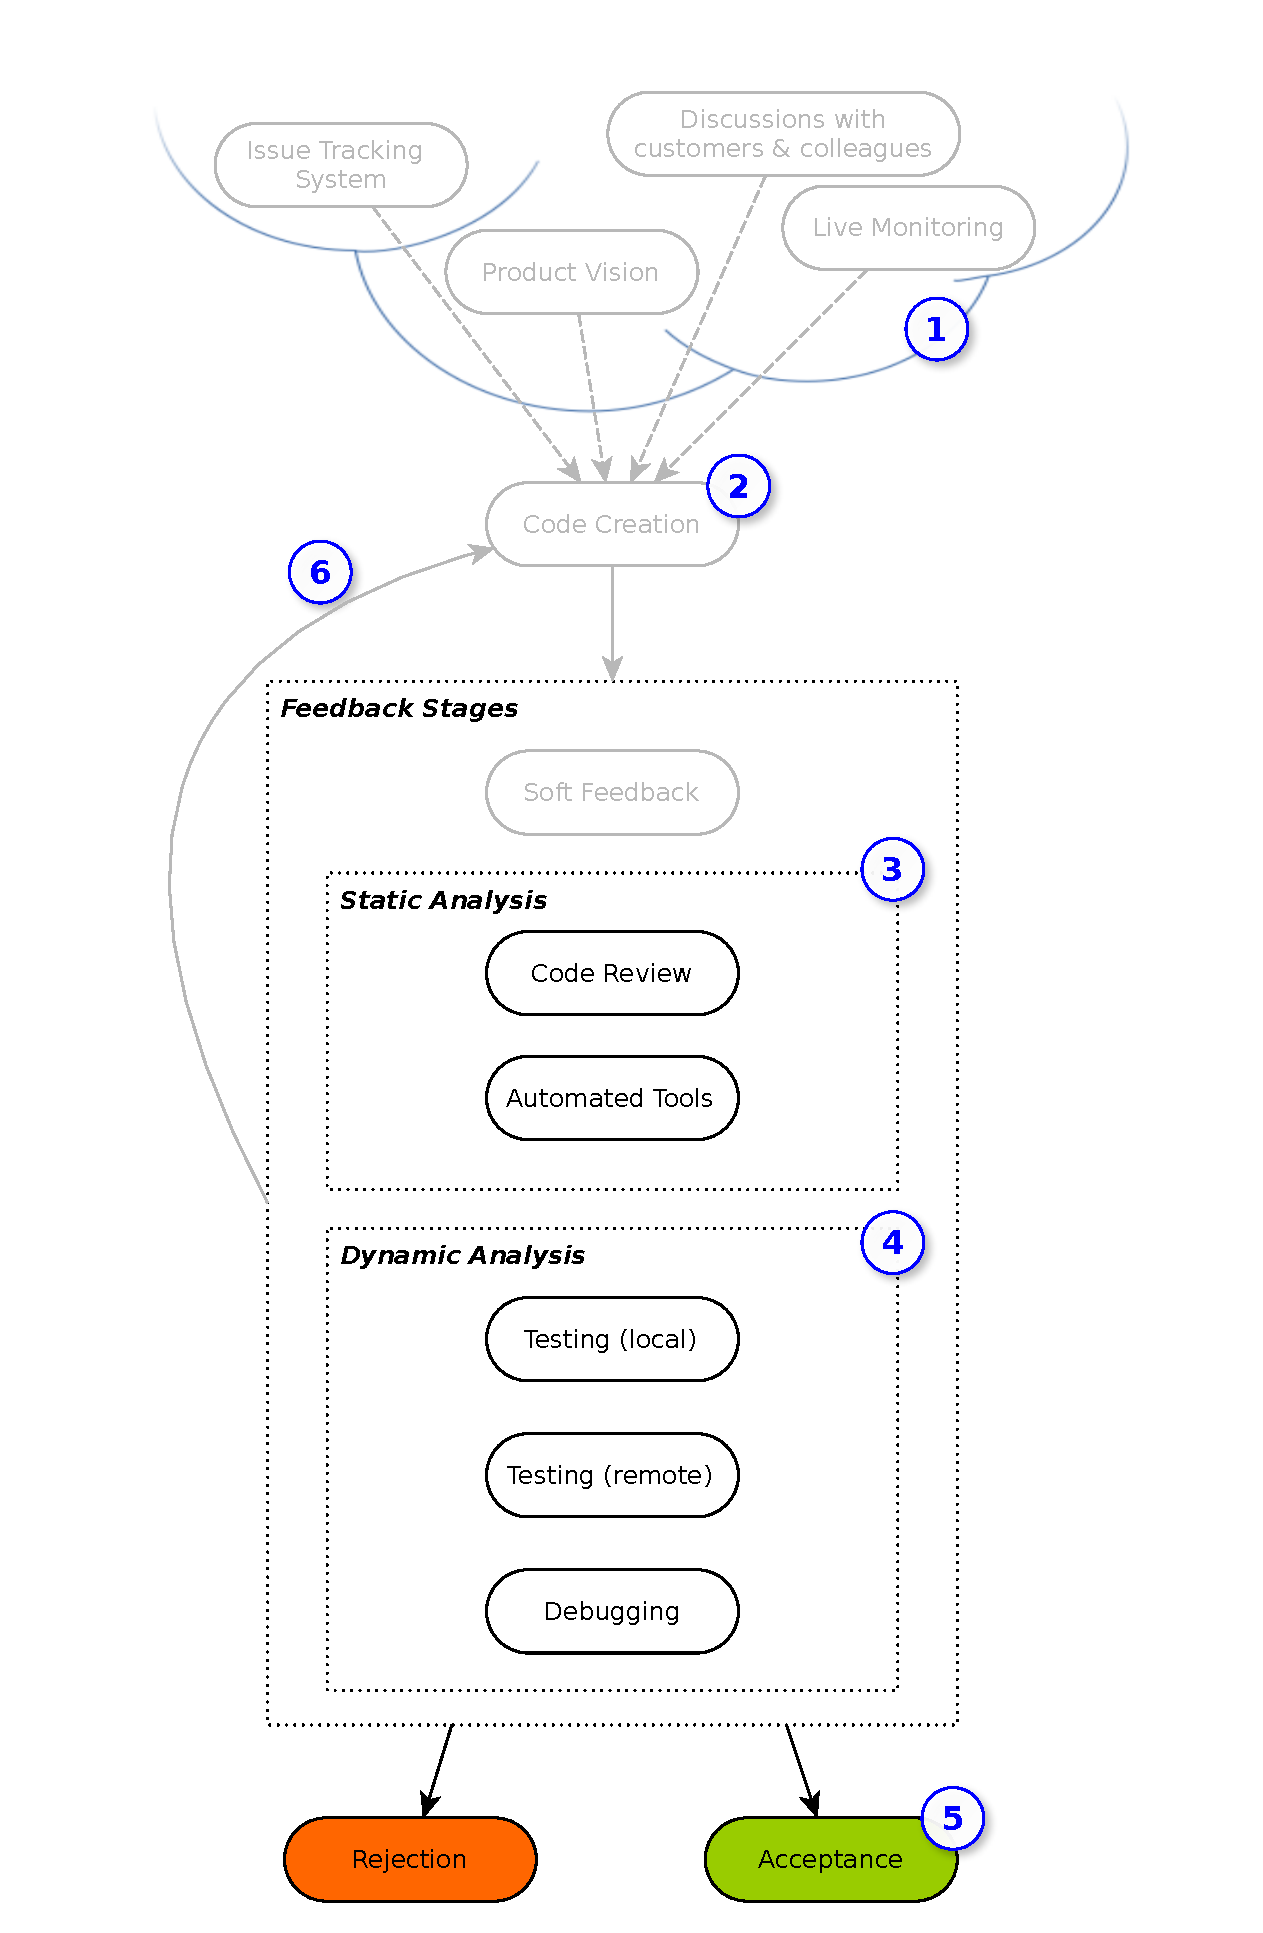
\includegraphics[width=0.65\columnwidth]{development_model_without_papers}
% 	\caption{The stages of the FDD model and their relationship to other
%           Software Engineering concepts.}
% 	\label{fig:devmodel}
% \end{figure}

We also have lists:

\begin{enumerate}
  \item Static Analysis~\circled{3} examines program artifacts or
    their source code without executing them~\cite{wichmann1995industrial}, while
 \item Dynamic Analysis~\circled{4} relies on information gathered from their
   execution~\cite{cornelissen2009systematic}.
\end{enumerate}

Or boxes:

\begin{framed}
This thesis is concerned with the empirical assessment of the state of the art of how developers
drive software development with the help of feedback loops. \cite{boyer2020dynamics}
\end{framed}

Or code:
\begin{lstlisting}[caption={\textsc{TrinityCore}},label={lst:e1}]
 x += other.x;
 y += other.y;
 z += other.y;
\end{lstlisting}


I hope this helps you get started!
Moritz

First time should be long: \gls{GCD}
Next time should be short: \gls{GCD}


\chapter{Background on Modeling and Control of Soft Robots}\label{chp:background}
\section{Kinematic Parametrizations}
\section{Dynamic Modeling}
\section{Model-based Controllers}

\chapter{Towards Quantifying the Safety of Soft Robots}
\label{chp:safetymetric}

\begin{foreword}
    % Traditionally, most effort in the robotics community has been on achieving safety through computational intelligence, i.e., by constraining motions to remain in a safe set of states, avoid obstacles, and compliant controllers such as impedance control. One of the most interesting and promising aspects of soft robots, on the other hand, is that their embodied intelligence contributes passive compliance to the system. However, in existing literature, the effect on the overall safety of the entire soft robotic system has not been thoroughly investigated or quantified. This lack of safety metric for soft robotics prevents us from considering it during the design process leading to either to badly performing and/or unsafe designs. This chapter proposes a safety metric for soft robots that captures both the embodied intelligence (i.e., the passive behavior) and the computational intelligence (i.e., the controller) of the system, allowing us, for the first time, to investigate quantitatively the effect on each on the overall safety and performance.
    Traditionally, efforts in the robotics community have focused on achieving safety through computational intelligence. This includes constraining motions to remain within safe state sets, avoiding obstacles, and employing compliant controllers such as impedance control. In contrast, one of the most intriguing and promising features of soft robots is their embodied intelligence, which provides passive compliance to the system. Despite this promise, existing literature has yet to thoroughly investigate or quantify the impact of embodied intelligence on the overall safety of soft robotic systems. The absence of a dedicated safety metric for soft robotics hampers the design process, often leading to underperforming or unsafe designs. This chapter introduces a safety metric for soft robots that captures both the embodied intelligence (i.e., the passive behavior) and computational intelligence (e.g., controller) of the system. For the first time, this allows for a quantitative evaluation of their combined effects on system safety and performance.
\end{foreword}

\blfootnote{This chapter is partly based on \faFileTextO~\emph{\textbf{M. Stölzle}*, N. Pagliarani*, F. Stella*, J. Hughes, C. Laschi, D. Rus, M. Cianchetti, C. Della Santina, and G. Zardini (2025). Safe yet Effective Soft Robots via Holistic Co-Design. In Nature Machine Intelligence, \textbf{\emph{In Preparation}}}.

\nth{1}-author contributions: M. Stölzle conceived and implemented the safety metric and all other content presented in this chapter, including the writing, except for Figures \ref{fig:safetymetric:safety_metric_applications} \& \ref{fig:safetymetric:injury_severity_criterion}. 
}

\pagebreak

\begin{abstract}
    % Original version
    % As we work towards integrating robots into human-centric environments, we need to ensure safety while not overly restricting the robot design and/or behavior design. The quest for making robots safer has existed for a long time, with efforts mostly focused on making their control safer and more compliant. Soft robots offer a fundamentally different take on this topic by achieving safety through passive compliance of the entire body. While there has been tremendous research progress in the domain of soft robotics in recent years, ranging from novel actuators to effective model-based control approaches, one of the fundamental promises, safety, has rarely been studied in a principled fashion. In particular, we notice the lack of a quantitative metric to assess how \emph{safe} a soft robot really is. Adding on, we notice that most works take too much of a simplified approach to this topic, equaling safety to material softness. Instead, in reality, the safety of the closed-loop system is influenced by many aspects such as topology, controller, etc, leading to suboptimal soft robot designs that are, for example, too soft to carry practical payloads. Instead, a quantitative safety metric would allow designers to analyze and exploit the safety-vs-performance tradeoff and identify more performant designs while still meeting the necessary safety requirements. In this chapter, we devise requirements a safety metric for soft robots would need to meet. Subsequently, we propose a safety metric that measures the injury severity based on the maximum contact pressure experienced during a collision, as it is already the standard for collaborative robots. Finally, we analyze the safety of continuum soft robots modeled according to the \gls{PCS} parametrization and devise a few simple recommendations for safe soft robot design.
    % short version by ChatGPT
    % Integrating robots into human-centric environments requires ensuring safety without overly restricting the robot's behavior. While soft robotics inherently enhances safety by adding passive body compliance, its core promise—safety—has been largely understudied in a principled manner. Most research equates safety to material softness, overlooking the complex interplay of factors like topology and control systems, which often leads to suboptimal designs that may be too soft to carry practical payloads. A quantitative safety metric could address this issue, enabling designers to balance the trade-off between safety and performance, thus achieving more effective designs while meeting safety requirements. In this chapter, we identify the requirements for a meaningful safety metric for soft robots and propose one based on maximum contact pressure during collisions, consistent with standards for collaborative robots. Using this metric, we analyze the safety of continuum soft robots modeled with the \gls{PCS} parametrization. Finally, we provide recommendations for designing safer soft robots that optimize both performance and safety.
    % longer version by ChatGPT
    As we work toward integrating robots into human-centric environments, it is crucial to ensure safety without overly constraining robot design or behavior. Efforts to enhance robot safety have a long history, primarily focusing on improving control systems to make them safer and more compliant. Soft robots offer a fundamentally different approach to this challenge by achieving safety through the passive compliance of their entire structure. Despite significant advancements in soft robotics over recent years—spanning novel actuators to sophisticated model-based control methods—one of the field’s core promises, safety, has rarely been systematically studied. Notably, there is a lack of a quantitative metric to evaluate how safe a soft robot truly is.
    Moreover, most existing studies oversimplify the concept of safety, equating it to material softness. In reality, the safety of a closed-loop system depends on multiple factors, such as topology and control strategies. This narrow focus often results in suboptimal soft robot designs, such as robots that are too soft to handle practical payloads effectively. A quantitative safety metric would enable designers to evaluate and balance the tradeoff between safety and performance, leading to more optimal designs that meet safety requirements without sacrificing functionality.
    In this chapter, we outline the essential criteria for a safety metric tailored to soft robots. We then propose a metric that assesses injury severity based on the maximum contact pressure during a collision, aligning with established standards for collaborative robots. Finally, we characterize the proposed safety metric on continuum soft robots modeled using the \gls{PCS} parametrization. % and provide practical recommendations for designing safe soft robots.
\end{abstract}

%% Start the actual chapter on a new page.
\newpage

\section{Introduction}
% As already mentioned in Chapter~\ref{chp:introduction}, the soft robotics community frequently emphasizes the "intrinsic safety" and natural compliance of soft robots~\citep{abidi2017intrinsic} - particularly as a differentiating factor from traditional rigid robots and even \glspl{Cobot}~\citep{laschi2014soft, rus2015design, yasa2023overview}.
% However, against scientific best practices, the safety improvement of continuum soft robots compared to rigid manipulators have, to the best of our knowledge, never been quantified. 
% We think that it is crucial for the community to thoroughly validate intrinsic compliance as a very prominent motivation for soft robots in order to justify continued spending into research and development of soft robots~\citep{hawkes2021hard}.
\dropcap{A}s noted in Chapter~\ref{chp:introduction}, the soft robotics community often highlights the “intrinsic safety” and natural compliance of soft robots~\citep{abidi2017intrinsic} as a key advantage over conventional rigid robots and even \glspl{Cobot}~\citep{laschi2014soft, rus2015design, yasa2023overview}. Yet, in contrast to established scientific practices, the safety improvements of continuum soft robots compared to rigid manipulators have not been rigorously quantified. We believe it is essential for the community to validate intrinsic compliance as a fundamental benefit of soft robots, thereby justifying continued investments in their research and development~\citep{hawkes2021hard}.

% Furthermore, as designers currently have no clear guideline for the “right” level of safety, we find that currently they prioritizes an overly soft material for safety.
% Indeed, designers have treated this challenge as a balance between precision and softness, assuming that increasing material compliance inherently improves safety.
% However, \emph{too soft} material choices can compromise the effectiveness of the soft robot, leading to imprecise, oscillatory motions, limited payload capacity, and the inability to exert sufficient forces on the environment~\citep{iida2011soft, cianchetti2013stiff, mazzolai2022roadmap, majidi2014soft, hawkes2017soft}.
% Indeed, we argue that precision vs. softness is an oversimplification, because the safety of soft robots is a function of both body (e.g., morphology) and brain (e.g., control and perception systems).
% Formalizing and quantifying such safety vs. performance tradeoff would enable designers to identify a good balance between the two and maximizing the performance while guaranteeing the necessary safety.
% Indeed, we we anticipate that removing this road-block would lead to more optimal and performant soft robot designs while preserving safety, which is in particular crucial in human-centered environment.
Moreover, in the absence of clear guidelines for determining the optimal level of safety, designers currently tend to favor overly compliant materials. Many treat the challenge as a trade-off between performance/precision and softness, assuming that higher material compliance automatically results in enhanced safety. However, choosing materials that are too soft can undermine the robot’s effectiveness, leading to imprecise or oscillatory motions, reduced payload capacity, and an inability to apply sufficient force to the environment~\citep{iida2011soft, cianchetti2013stiff, mazzolai2022roadmap, majidi2014soft, hawkes2017soft}. We argue that framing the issue as merely a balance between performance and softness oversimplifies the problem, since the safety of soft robots depends on both their body (e.g., morphology) and their brain (e.g., control and perception systems). Formalizing and quantifying this safety–performance trade-off would enable designers to find an optimal balance that maximizes performance while ensuring the necessary safety, a consideration that is particularly critical in human-centered environments.

% Apart from \emph{safety-aware design}, we expect that a safety metric would also be very beneficial for other purposes such as \emph{safety certification} of a soft robotic design or \emph{safety-aware control} where the controller chooses its actions such as that the required safety levels are always met.
% After detailing such potential applications of a safety metric for soft robots in more detail, we devise requirements that a safety metric would need to meet in order to be suitable for the mentioned applications.
% Subsequently, we then propose a new model-based safety metric for soft robots by building an injury criterion on top of the existing ISO norms for collaborative robots~\citep{Isots_15066_2016} while modifying the underlying model to account for the essential characteristics of soft robots, such as the elastic structure that deforms under the influence of internal actuation and external forces, and the potential of collisions along its entire body.
% After modeling the contact model and the collision dynamics between soft robots and humans, we consider analog to ISO/TS 15066:2016~\citep{iso2016collaborative}, the maximum contact pressure experienced during the collision as a proxy for the injury severity. Instead of requiring computationally expensive simulations, we devise a conservative approximation of the collision dynamics, which allows us to determine the maximum contact pressure in closed form.
% Importantly, the proposed safety metric considers the safety of the closed-loop system, which allows us to take the control policy into account when assessing the severity of the injury.
% The safety metric comes in two flavors: \gls{SRISC} computes the injury severity for a known soft robot state, control input, and contact geometry (e.g., point along the soft robot body of contact and collision direction) and is particularly well suited for \emph{safety-aware control} applications. 
% When we want to judge the safety of a soft robot design, we can instead compute the \gls{SRDHC}, which considers all possible contact geometries, soft robot states, etc., within the given operating conditions. We envision the \gls{SRDHC} the metric of choice for \emph{safety-aware design} and \emph{design safety certification}.
Beyond \emph{safety-aware design}, we expect that a comprehensive safety metric will be invaluable for other applications, such as the \emph{safety certification} of soft robotic designs and \emph{safety-aware control}, where the controller adjusts its actions to continuously meet required safety levels. After discussing these potential applications in detail, we establish the requirements a safety metric must satisfy for these purposes. We then introduce a new model-based safety metric for soft robots by extending the injury criterion from the existing ISO norms for collaborative robots~\citep{iso2016collaborative}. Our approach modifies the underlying model to capture key characteristics of soft robots, such as their elastic structures—which deform under internal actuation and external forces—and the possibility of collisions occurring along their entire body. By modeling the contact interactions and collision dynamics between soft robots and humans, and analogously to ISO/TS 15066:2016~\citep{iso2016collaborative}, we use the maximum contact pressure during a collision as a proxy for injury severity. Instead of relying on computationally expensive simulations, we develop a conservative approximation of the collision dynamics that allows us to compute the maximum contact pressure in closed form. Importantly, our safety metric considers the closed-loop system dynamics, incorporating the control policy when assessing injury severity. It is offered in two variants: the \gls{SRISC}, which calculates injury severity for a known soft robot state, control input, and contact geometry (e.g., the specific point of contact and collision direction), making it especially suited for \emph{safety-aware control} applications; and the \gls{SRDHC}, which evaluates safety across all possible contact geometries and robot states within a given operating envelope. We envision the \gls{SRDHC} as the metric of choice for both \emph{safety-aware design} and \emph{design safety certification}.
\section{Towards Quantifying the Safety of Soft Robots}
In the following, we will motivate the need for a quantitative safety metric by showcasing future applications that such a metric would enable.
This will then allow us to define a list of requirements for characteristics that a safety metric needs to exhibit.
Subsequently, we contextualize the topic by reviewing the literature on how safety has been assessed and quantified in the realm of robotics before, where almost all prior work is on the safety of industrial and collaborative rigid robotic manipulators.

\begin{figure}
    \centering
    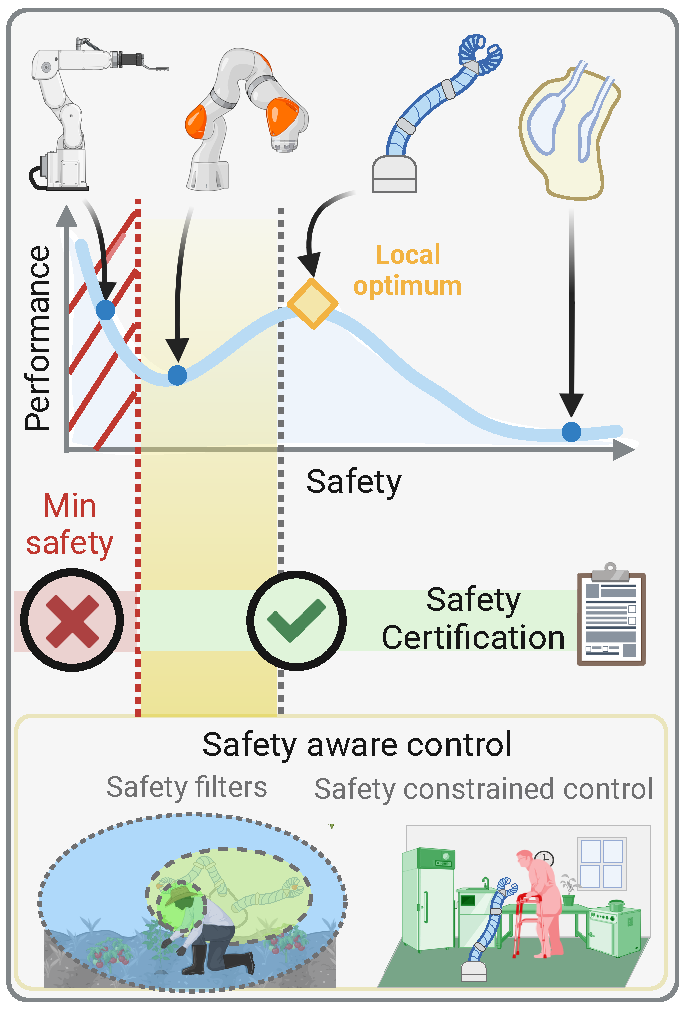
\includegraphics[width=0.5\linewidth]{safetymetric/figures/safety_metric_applications.pdf}
    \caption{Future applications that a quantitative safety metric for soft robots would enable. \textbf{Top:} Here, we showcase how the safety metric could be used for \emph{safety-aware design optimization} and, particularly, for analyzing and exploiting the performance vs. safety tradeoff. Subsequently, the safety metric could be used for certifying a given design as \emph{safe} for the respective application. \textbf{Bottom:} The safety metric could also be used for \emph{safety-aware control} - either by filtering the outputs of the controller without safety guarantees or by explicitly including the safety requirements as constraints during the optimization of the control input sequence (e.g., MPC, Control Barrier Functions).}
    \label{fig:safetymetric:safety_metric_applications}
\end{figure}

\subsection{Potential Applications for a Safety Metric}\label{sub:safetymetric:safety_metric_applications}
% We envision a safety metric for soft robots to unlock a variety of applications that we showcase in Fig.~\ref{fig:safety_metric_applications}, and that can be grouped into the domains of \emph{safety-aware control} and \emph{safety-aware design}.
We envision a safety metric for soft robots that will enable a variety of applications, as illustrated in Fig.~\ref{fig:safetymetric:safety_metric_applications}. These applications can be categorized into two main domains: \emph{safety-aware control} and \emph{safety-aware design}.

% In the domain of \emph{safety-aware control}, we assume the soft robotic design to be given, and we strive to control the actions of the soft robot in such a way that the achieved safety level remains within an acceptable range. We remark that this does not exclude contact or even collision with the environment. Instead, we strive to guarantee that these collisions do not cause any (significant) injuries. Examples include \emph{safety filters}~\cite {bertino2023prescribed} that allow us to use performant control policies that do not explicitly consider the safety constraints (e.g., RL) and still guarantee safety by filtering/saturating the control input. Alternative techniques such as MPC~\citep{hewing2020learning} or Control Barrier Functions~\citep{ames2016control}, which we refer to as \emph{safety-constrained control}, allow us to take the safety constraints directly into account when devising the control input.
In the realm of \emph{safety-aware control}, we assume the soft robotic design is already established and focus on controlling its actions to maintain an acceptable safety level. This approach does not preclude contact or collisions with the environment; rather, it ensures that such interactions do not result in significant injuries. Examples include \emph{safety filters}~\citep{bertino2023prescribed}, which allow the use of high-performance control policies (such as \gls{RL}) that do not explicitly account for safety constraints while still guaranteeing safety by filtering or saturating the control input. Alternative methods like \gls{MPC}~\citep{hewing2020learning} or Control Barrier Functions~\citep{ames2016control}—referred to as \emph{safety-constrained control}—integrate safety constraints directly into the control strategy.

% Another avenue that would be unlocked by a safety metric is \emph{safety-aware design}, which would include assessing an integrated soft robot design for its safety. Specifically, we consider here two subcategories: \emph{safety-aware design optimization} would consider safety when developing/optimizing the soft robot design either by means of inequality constraints (i.e., a minimum safety needs to be guaranteed) or by maximizing safety through the cost function.
% After a design is finalized, \emph{safety certification} would allow manufacturers to certify their product as being sufficiently safe for the respective applications (e.g., healthcare, agri-food, manufacturing, etc.). This is well-aligned with established safety standards for collaborative rigid robots as defined in ISO/TS 15066:2016~\citep{Isots_15066_2016}.
Another promising direction unlocked by a safety metric is \emph{safety-aware design}, which involves evaluating an integrated soft robot design for its safety. We see this as comprising two subcategories: \emph{safety-aware design optimization}, which incorporates safety into the design process either through inequality constraints (ensuring a minimum safety level) or by maximizing safety via the cost function; and \emph{safety certification}, where, after a design is finalized, manufacturers can certify that their product meets the necessary safety standards for specific applications (e.g., healthcare, agri-food, manufacturing, etc.). This approach aligns well with established safety standards for collaborative rigid robots as defined in ISO/TS 15066:2016~\citep{Isots_15066_2016}.

\subsection{Requirements for a Soft Robotic Safety Metric}\label{sub:safetymetric:safety_metric_requirements}
% In the following, we will list some requirements that, in our opinion, a safety metric needs to meet in order to be well suited for the applications listed in Sec.~\ref{sub:safetymetric:safety_metric_applications}.
% First (1), the metric shall consider the dynamics inherent to continuum soft robots and their particular characteristics. For example, one of the main differences between rigid and soft manipulators is that free-moving joints with integrated motors are replaced by an elastic structure that deforms under the influence of internal actuation and external forces. Therefore, any safety metric needs to crucially consider the elastic and inertial characteristics of the soft robot that are generated by the distributed material along its backbone.
% Secondly (2), the safety metric shall consider not just collision at the end-effector but instead anywhere along the body of the soft robot. This is a significant difference to the existing safety metrics for rigid/collaborative robots, which, for simplicity, usually only consider collisions at the end-effector as we would expect there the largest motion velocities~\citep{haddadin2011safe, Isots_15066_2016}. Instead, soft robots exhibit large Cartesian stiffnesses close to their proximal end, thus requiring us to consider the safety of collisions anywhere along the backbone.
% Next, (3) any simplifying assumptions shall lead to a conservative estimate of the achieved safety. For example, soft robot models underlying the safety metric would likely use a finite-dimensional approximation of the continuum shape; instead, in reality, flexible structures such as soft robots exhibit infinite degrees of freedom~\citep{della2023model, armanini2023soft}. Therefore, we would like any safety metric making use of finite-dimensional approximations to underestimate instead of overestimate the safety of the design.
% Fourthly (4), the computation of the safety metric shall be computationally tractable, which is essential for safety-aware control and design applications, where evaluations on the scale of sub-seconds and seconds are necessary.
% Finally, we end with a few desirable characteristics: (5) some applications, such as safety-aware control or safety-aware design, might benefit from the differentiability of the safety metric with respect to design parameters, robot states, and control inputs; (6) ideally, the safety metric shall also consider how \emph{safe} the soft robot's design (e.g., friendly-looking) and behavior (e.g., smooth and predictable movements) is perceived by the user. In addition to user studies, the evaluation of this metric might be assisted by VLMs.
In the following, we outline several requirements that, in our opinion, a safety metric must satisfy to be well-suited for the applications described in Sec.~\ref{sub:safetymetric:safety_metric_applications}. First (1), the metric should account for the dynamics inherent to continuum soft robots and their unique characteristics. For example, a primary difference between rigid and soft manipulators is that free-moving joints with integrated motors are replaced by a compliant structure that deforms under internal actuation and external forces. Consequently, any safety metric must consider the elastic and inertial properties generated by the distributed material along the robot’s backbone.
%
Secondly (2), the safety metric must evaluate collisions occurring anywhere along the soft robot’s body—not just at the end-effector. This represents a significant departure from existing safety metrics for rigid or collaborative robots, which often focus solely on the end-effector due to its typically higher motion velocities~\citep{haddadin2009requirements, haddadin2011safe, Isots_15066_2016}. In contrast, soft robots exhibit high Cartesian stiffness near their proximal end, making it necessary to assess safety along the entire structure.
% 
Next (3), any simplifying assumptions should yield a conservative safety estimate. For instance, while soft robot models used in the metric might employ a finite-dimensional approximation of the continuum shape, in reality, these flexible structures possess infinite degrees of freedom~\citep{della2023model, armanini2023soft}. Therefore, a safety metric based on such approximations should tend to underestimate rather than overestimate the design’s safety.
% 
Fourthly (4), the computation of the safety metric must be tractable, which is essential for safety-aware control and design applications that require evaluations on sub-second to second timescales, respectively.
% 
Finally, we highlight a few desirable characteristics: (5) in applications such as safety-aware control or design, it is advantageous if the safety metric is differentiable with respect to design parameters, robot states, and control inputs; and (6) ideally, the metric should also reflect how “safe” the soft robot’s design (e.g., its friendly appearance) and behavior (e.g., smooth and predictable movements) are perceived by users. In addition to user studies, the evaluation of this metric might be enhanced by leveraging \glspl{VLM}~\citep{touvron2023llama, grattafiori2024llama}.

\subsection{Background on Injury Risk Criteria for Robotic Manipulators}

\begin{itemize}
    \item Give a motivation for why the robotics community strives to quantify safety/injury risk (e.g., optimizing designs and controllers to make them more human-friendly, safety-aware control, etc.).
    \item Give an overview of the trailblazing literature on measuring the injury risk of rigid robots.
    \item Mention the ISO norm that establishes the standards for safe, collaborative robots.
    \item List the existing attempts to assess the safety of soft robots and why they are not sufficient (e.g., too simplistic models, not taking into account the control, lacking a contact model, etc.)
    \item List some of the initial attempts to give designers an idea of which factors influence the safety of soft robots (e.g.,~\citep{abidi2017intrinsic}).
\end{itemize}

\textcolor{red}{Stucture: \begin{enumerate}
    \item Motivation for measuring safety: selecting suitable design, defining constraints that guarantee safety (i.e., ISO norms), and safety-aware control and motion planning
    \item Stress that this is a well-established line of research in (rigid) robotics involving both conceptual and experimental analysis
    \item Modes of impact and injury: constrained vs. unconstrained (human), static vs. dynamic, sharp surfaces, different body parts, etc.~\citep{haddadin2009requirements}
    \item Injurity severity criterias: the first were based on automobile crash models (HIC), but found to be unsuitable as they are calibrated for higher velocities and inertias that are not even relevant for rigid robots. In particular, taking the head acceleration as a injury criteria is not suitable, as not in practice reached, even when robots are moving at 2m/s. Furthermore, it mostly focuses on the question of fatale impacts. Instead, other injury modes, even if not fatal, become relevant as (rigid) robots can still cause bones to break and other significant injuries at their speeds. There exist specialized injury severity criteria inspired by biomechanics for the various body parts. For example, body parts have different contact stiffnesses and injury is (most likely) caused when different thresholds are exceeded (e.g., penetration depth, maximum force, energy density, acceleration). However, it seems that most of them are correlated with the the maximum force experienced during impact and that the maximum force generalizes the best across body parts.
    \item Mention ISO/TS 15066:2016 (Collaborative robots) and ISO/PAS 5672:2023
    \item Safety metrics for soft robots: basically not existing, only~\citep{abidi2017intrinsic}, but only super-simplified beam model. A safety metric is especially important for soft robots as we continuously stress the inherent safety of soft robots, so we also need to be able to quantify it.
\end{enumerate}}

Various aspects have motivated the robotic community to try to assess the safety of our robots~\citep{de2008atlas, van2018spatial}: 
First of all, understanding the important factors influencing safety allows us to make robotic designs and control algorithms safer~\citep{bicchi2004fast, zinn2004new}. 
Secondly, quantifying the injury risk stemming from a robot allows the establishment of minimal safety standards and specifically constraints on the design and actuation that guarantee safe deployment of the robots, as done, for example, in ISO 10218-1:2011~\citep{iso2011robots} for industrial robots and ISO/TS 15066:2016~\citep{Isots_15066_2016} for collaborative robots. This allows the designers and manufacturers of robots to certify that their design is \emph{safe}, which is, in turn, crucial for successful adoption by industrial customers and consumers.
Thirdly, modeling the injury risk of robots and explicitly setting operation constraints that guarantee safety enables safety-aware control~\citep{lacevic2011safety, zanchettin2015safety, mansfeld2018safety}, motion planning~\citep{lacevic2022safe, pupa2024efficient} and also the deployment of safety filters~\citep{hewing2020learning, bertino2023prescribed}.

% Before improving the safety of (collaborative) robots, we first need to understand the important factors influencing the injury risk and be able to compare different robot design w.r.t. to their achieved safety level~\citep{de2008atlas}.
For the reasons mentioned above, quantifying the safety and associated injury risk has been a longstanding research topic, with most effort centered on determining the safety of collaborative rigid robotic manipulators~\citep{zinn2004playing, bicchi2004fast, haddadin2009requirements, mansfeld2018safety}.
\section{A Metric for Quantifying the Safety of Soft Robots}
Thereafter, we propose a quantitative safety metric for \emph{blunt} contacts~\citep{haddadin2011safe} between soft robots and humans that captures the particular characteristics that continuum soft robots exhibit (e.g., elasticity, actuation through their structure, Cosserat rod dynamics, etc.).
Importantly, the presented safety metric fulfills all the mandatory requirements that we laid out previously. % (e.g., based on a soft robotic dynamical model, computationally tractable, differentiable, etc.).
First, we state the necessary background on soft robotic dynamics and contact models. Subsequently, we derive the dynamics of a collision between the continuum soft robot and the human (body part).
Next, we propose two flavors of the safety metric: (i) the \glsxtrfull{SRISC} captures the injury risk for a \emph{given} contact geometry, soft robot state, and actuation sequence. We envision this criterion to be useful for control applications with safety guarantees.
The second flavor, (ii) the \glsxtrfull{SRDHC}, captures the inherent safety of an integrated soft robot design (e.g., also considering the control policy) and leverages the \gls{SRISC} for estimating the maximum injury risk over all possible contact geometries, feasible robot states, and actuation sequences.
Apart from the procedure for formulating this safety metric, one of the key innovations here is that we identify a closed-form solution to the collision dynamics, which renders the computation of the \gls{SRISC} to be computationally tractable.

\subsection{Background on Soft Robot Dynamics and Contact Model}
Following the Cosserat rod theory, we can capture the kinematic behavior of slender structures such as continuum soft robots by considering the deformations of the robot's backbone. As the 1D spatial deformations of this backbone are still an infinite-dimensional problem, the field has developed many methods, such as \gls{PCC}~\citep{webster2010design}, \gls{PCS}~\citep{renda2018discrete}, and \gls{GVS}~\citep{renda2020geometric}, to describe such deformations with a finite number of finite vector of configuration variables $q \in \mathbb{R}^n$. The associated forward kinematic model then allows us to define the geometric positional Jacobian $J_\mathrm{p}(q, s) \in \mathbb{R}^{3 \times n}$, where $s \in (0,L]$ is the backbone abscissa/coordinate and $L$ is the length of the entire continuum structure.
Independent of the specific chosen kinematic model, the \gls{EOM} of a continuum soft robot can often be stated as~\citep{armanini2023soft, della2023model}
\begin{equation}\label{eq:safetymetric:soft_robot_configuration_space_dynamics}
    M(q) \, \ddot{q} + C(q, \dot{q}) \, \dot{q} + \partial_{q} \, \mathcal{U}(q) + D \, \dot{q} = A(q) \, \tau + \tau_\mathrm{c},
\end{equation}
$M(q) \in \mathbb{R}^{n \times n}$ and $C(q, \dot{q}) \in \mathbb{R}^{n \times n}$ considers the inertial and Coriolis effects of the soft robot system, respectively.
$\partial_{q} \, \mathcal{U}(q) \in \mathbb{R}^n$ captures the forces stemming from the potential $\mathcal{U}(q): \mathbb{R}^n \to \mathbb{R}$.
Often times, the potential forces simplify to $\partial_{q} \, \mathcal{U}(q) =  G(q) + K q$, where $G(q) \in \mathbb{R}^{n}$ describes the gravitational forces, and $K \succ 0 \in \mathbb{R}^{n \times n}$ is the stiffness matrix.
Dissipation is integrated through the damping matrix $D \succ 0 \in \mathbb{R}^{n \times n}$.
$\tau(t,q,\dot{q}) \in \mathbb{R}^{m}$ contributes the actuation (determined by a control policy) that acts through the linear map $A(q) \in \mathbb{R}^{n \times m}$ on the generalized coordinates.

The term $\tau_\mathrm{c} \in \mathbb{R}^n$ collects all contributions by external contact forces on the generalized coordinates.
In the following, we will assume that the soft robot is only in contact with the human at one discrete point and that only pure forces are reflected between the bodies during the contact (i.e., no Cartesian torques).
Specifically, we assume that the contact occurs at the backbone abscissa $s_\mathrm{c} \in (0, L]$ and that the contact exhibits a constant surface normal of $n_\mathrm{c} \in \mathcal{S}^3$ which is a unit vector and, with that, $\mathcal{S}^3 = \{ n_\mathrm{c} \in \mathbb{R}^3: \lVert n_\mathrm{c} \rVert_2 = 1 \}$.
We now describe with $\delta_\mathrm{c} > 0$ a penetration between the soft robot and the soft tissue of the human.
Then, the generalized torque acting on the soft robot as a consequence of the contact is given by $\tau_\mathrm{c} = -J^\top(q,s_\mathrm{c}) \, n_\mathrm{c} \, f_\mathrm{c}(\delta_\mathrm{c}, \dot{\delta}_\mathrm{c}) = -J_\mathrm{c}^\top(q, s_\mathrm{c}, n_\mathrm{c}) \, f_\mathrm{c}(\delta_\mathrm{c}, \dot{\delta}_\mathrm{c})$, where $f_\mathrm{c}(\delta_\mathrm{c}, \dot{\delta}_\mathrm{c}) \in \mathbb{R}_{\geq 0}$ is the scalar non-negative contact force.
In the following, we will frequently omit the dependency of symbols, such as $J_\mathrm{c}(q)$, on the $(s_\mathrm{c}, n_\mathrm{c})$ to simplify the notation.
While the formulation that we use in this chapter for formulating the safety metric is compatible with many of the contact models that have been studied in the literature, such as Hunt-Crossley~\citep{hunt1975coefficient, aouaj2021predicting}, Hertz~\citep{johnson1987contact, park2011designing, she2020comparative}, etc., we will mainly focus in the following on a linear spring-damper contact model~\citep{iso2016collaborative, haddadin2009requirements} given by
\begin{equation}
    f_\mathrm{c}(\delta_\mathrm{c}, \dot{\delta}_\mathrm{c}) =
    \begin{cases}
        0 & \delta_\mathrm{c} \leq 0,\\
        k_\mathrm{c} \, \delta_\mathrm{c} + d_\mathrm{c} \, \dot{\delta}_\mathrm{c} & \delta_\mathrm{c} > 0,\\
    \end{cases}
\end{equation}
where $k_\mathrm{c} \in \mathbb{R}_{>0}$ is the contact stiffness and $d_\mathrm{c} \in \mathbb{R}_{\geq 0}$ is the contact damping coefficient.
If we assume the soft robot surface material and the human soft tissue to have spring constants and damping coefficients of $k_\mathrm{R,surf}$, $k_\mathrm{H,st}$ and $d_\mathrm{R}$, $d_\mathrm{H}$, respectively, then we can connect the spring-dampers in series
\begin{equation}
    k_\mathrm{c} = \left (\frac{1}{k_\mathrm{R,surf}} + \frac{1}{k_\mathrm{H,st}} \right )^{-1},
    \qquad
    d_\mathrm{c} = \left (\frac{1}{d_\mathrm{R}} + \frac{1}{d_\mathrm{H}} \right )^{-1}.
\end{equation}
Please note that the effective spring constant of many human body parts is reported in ISO/TS 15066:2016~\citep{iso2016collaborative}.

\subsection{Collision Dynamics}
We now progress towards a formulation of the collision dynamics as motions of the soft robot and the human body part along the contact surface normal $n_\mathrm{c}$.

First, we describe the motion of the contact point of the soft robot with position and velocity $x_\mathrm{R}, \dot{x}_\mathrm{R} \in \mathbb{R}$.
We can project the dynamics of \eqref{eq:safetymetric:soft_robot_configuration_space_dynamics} into this 1D motion through the expression $\dot{x}_\mathrm{R} = J_\mathrm{c} \, \dot{q}$ yielding the form~\citep{khatib1987unified, della2019exact, della2020model, stolzle2024guiding}
\begin{equation}
    \Lambda_\mathrm{c}(q) \, \Ddot{x}_\mathrm{R} + \eta_\mathrm{c}(q,\dot{q}) \, \dot{x}_\mathrm{R} + J_\mathrm{c,M}^{+\top}(q) ( \partial_{q} \, \mathcal{U}(q) + D \dot{q} ) = J_\mathrm{c,M}^{+\top}(q) \, A(q) \, \tau - f_{\mathrm{c}}(\delta_\mathrm{c}, \dot{\delta}_\mathrm{c}),
\end{equation}
where $J_\mathrm{c,M}^{+\top}(q, s_\mathrm{c},n_\mathrm{c}) = M^{-1}J_\mathrm{c}^\top(J_\mathrm{c} M^{-1} J_\mathrm{c}^\top)^{-1} \in \mathbb{R}^{n \times 1}$ is the dynamically consistent pseudo-inverse, $\Lambda_\mathrm{c}(q, s_\mathrm{c},n_\mathrm{c}) = (J_\mathrm{c} \, M^{-1} J_\mathrm{c}^\top)^{-1} \in \mathbb{R}^{1 \times 1}$ is the reflected inertia of the soft robot at the contact point~\citep{haddadin2009requirements, iso2016collaborative}, and $\eta_\mathrm{c}(q,\dot{q},s_\mathrm{c},n_\mathrm{c}) = \Lambda_\mathrm{c}(q) \, (J_\mathrm{c} M^{-1} C - \dot{J}_\mathrm{c}) \in \mathbb{R}^{1 \times n}$ collects the Cartesian Coriolis and centrifugal terms~\citep{khatib1987unified}.
As mentioned already previously, if not explicitly stated otherwise, we will in the following, to simplify the notation, drop the specific dependency on the contact geometry $(s_\mathrm{c}, n_\mathrm{c})$: $J_\mathrm{c,M}^{+\top}(q) = J_\mathrm{c,M}^{+\top}(q,s_\mathrm{c},n_\mathrm{c})$, $\Lambda_\mathrm{c}(q) = \Lambda_\mathrm{c}(q,s_\mathrm{c},n_\mathrm{c})$, etc.

Next, we move towards modeling the behavior of the human body part. In literature, the human body part is usually modeled as a point mass\footnote{Please note that the effective mass of various human body parts is reported in ISO/TS 15066:2016~\citep{iso2016collaborative}.} $m_\mathrm{H}$~\citep{haddadin2011safe, iso2016collaborative} that moves in 1D along the surface normal of the contact with state $(x_\mathrm{H},\dot{x}_\mathrm{H})$. Instead, we take here a conservative approach and assume that the human body is constrained in its motion with velocity $v_\mathrm{H} \in \mathbb{R}$ towards the soft robots (i.e., $m_\mathrm{H} \gg \Lambda(q) \: \forall q$). This represents the \emph{worst case}.
After the coordinate change $\delta_\mathrm{c}(t) = x_\mathrm{R}(t) - x_\mathrm{H}$, $\dot{\delta}_\mathrm{c} = \dot{x}_\mathrm{R}(t) + v_\mathrm{H}$, % where $x^{\mathrm{c}0} \in \mathbb{R}$ is the position of the initial contact, 
where $x_\mathrm{H} \in \mathbb{R}$ is the position of the soft tissue surface, and while only considering the case of contact (i.e., $\delta_\mathrm{c} \geq 0$), the collision dynamics are given by
\begin{equation}
    \Lambda_\mathrm{c}(q) \, \Ddot{\delta}_\mathrm{c} + \eta_\mathrm{c}(q,\dot{q}) \, \dot{\delta}_\mathrm{c} + J_\mathrm{c,M}^{+\top}(q) ( \partial_{q} \, \mathcal{U}(q) + D \dot{q} ) = J_\mathrm{c,M}^{+\top}(q) \, A(q) \, \tau - k_\mathrm{c} \, \delta_\mathrm{c} - d_\mathrm{c} \, \dot{\delta}_\mathrm{c}.
\end{equation}
We are now interested in identifying the maximum force $f_\mathrm{c}(t)$ that occurs during the entire time of the contact.
Therefore, we can neglect any damping forces, such as $d_\mathrm{c} \, \dot{\delta}_\mathrm{c}$ and $D \, \dot{q}$, as they dissipate energy, and, therefore, reduce the maximum contact force.
Furthermore, we assume that the Coriolis effects are sufficiently small and can be neglected as well.
Finally, we assume that the change of configuration during the collision is sufficiently small such that the dynamic matrices can be approximated as constant: 
\begin{equation}\label{eq:safetymetric:constant_reflected_inertia_and_actuation_matrix_definition}
    m_\mathrm{R} = \Lambda_\mathrm{c}(q_{\mathrm{c}}^0) \approx \Lambda_\mathrm{c}(q),
    \qquad
    A_\mathrm{c} = J_\mathrm{c,M}^{+\top}(q_{\mathrm{c}}^0) \, A(q_{\mathrm{c}}^0) \approx J_\mathrm{c,M}^{+\top}(q) \, A(q),
    \quad
    \forall \: t \geq t_\mathrm{c}^0,
\end{equation}
where the $q_{\mathrm{c}}^0$ is the configuration of the robot at the beginning of the contact.
The same assumption also allows us to linearize the potential forces of the soft robot with 
\begin{equation}\label{eq:safetymetric:collision_potential_forces}
    f_{\mathcal{U}} = J_\mathrm{c,M}^{+\top}(q) \, \partial_{q} \, \mathcal{U}(q) \approx \underbrace{J_\mathrm{c,M}^{+\top}(q_{\mathrm{c}}^0) \, \partial_{q} \, \mathcal{U}(q_{\mathrm{c}}^0)}_{f_{\mathcal{U}}^{\mathrm{c}0}} + \underbrace{\frac{\partial}{\partial q} J_\mathrm{c,M}^{+\top}(q) \, \partial_{q} \, \mathcal{U}(q) \Big |_{q=q_{\mathrm{c}}^0} \,  J_\mathrm{c,M}^{+}(q_{\mathrm{c}}^0)}_{k_\mathrm{R}}  \, \delta_\mathrm{c},
\end{equation}
where $k_\mathrm{R} \in \mathbb{R}$ is the local stiffness of the system against small perturbations and $f_{\mathcal{U}}^{\mathrm{c}0}$ are the potential forces present at the start of the contact.
Furthermore, we assume the actuation force to be constant, which can be easily accomplished by conservatively considering the maximum actuation force $f_\tau = \max_t \left | A_\mathrm{c} \, \tau(t) \right |$ that the robot experiences during the collision.
Integrating the stated assumptions into the \gls{EOM} results in the approximated collision dynamics (during contact)
\begin{equation}\label{eq:safetymetric:simplified_collision_dynamics}
    m_\mathrm{R} \, \Ddot{\delta}_\mathrm{c} + (k_\mathrm{R} + k_\mathrm{c}) \, \delta_\mathrm{c} = f_\tau - f_{\mathcal{U}}^{\mathrm{c}0}.
\end{equation}
To avoid computationally expensive simulations of the collision, we identify a closed-form solution to the collision dynamics
\begin{equation}\small\label{eq:safetymetric:collision_dynamics_cfs}
\begin{split}
    \delta_\mathrm{c}(t) =& \: \left (\delta_\mathrm{c}^0-\frac{f_\tau-f_{\mathcal{U}}^{\mathrm{c}0}}{k_\mathrm{R} + k_\mathrm{c}} \right ) \cos \left ( \sqrt{\frac{k_\mathrm{R} + k_\mathrm{c}}{m_\mathrm{R}}} \, t \right ) + \dot{\delta}_\mathrm{c}^0 \sqrt{\frac{m_\mathrm{R}}{k_\mathrm{R} + k_\mathrm{c}}} \, \sin \left ( \sqrt{\frac{k_\mathrm{R} + k_\mathrm{c}}{m_\mathrm{R}}} \, t \right ) + \frac{f_\tau-f_{\mathcal{U}}^{\mathrm{c}0}}{k_\mathrm{R} + k_\mathrm{c}},\\
    \dot{\delta}_\mathrm{c}(t) =& \: -\sqrt{\frac{k_\mathrm{R} + k_\mathrm{c}}{m_\mathrm{R}}} \left (\delta_\mathrm{c}^0 - \frac{f_\tau-f_{\mathcal{U}}^{\mathrm{c}0}}{k_\mathrm{R} + k_\mathrm{c}} \right ) \, \sin \left ( \sqrt{\frac{k_\mathrm{R} + k_\mathrm{c}}{m_\mathrm{R}}} \, t \right ) + \dot{\delta}_\mathrm{c}^0 \, \cos \left ( \sqrt{\frac{k_\mathrm{R} + k_\mathrm{c}}{m_\mathrm{R}}} \, t \right ),
\end{split}
\end{equation}
where we assume without loss of generality that $t_\mathrm{c}^0=0$ at the start of the collision, and $\delta_\mathrm{c}^0$ is the initial penetration depth, although generally $\delta_\mathrm{c}^0 = 0$.
The initial penetration velocity can be computed as a function of the configuration-space velocity as $\dot{\delta}_\mathrm{c}^0 = J_\mathrm{c}(q_{\mathrm{c}}^0) \, \dot{q}_{\mathrm{c}}^0 + v_\mathrm{H}$.

\begin{figure}[h!]
    \centering
    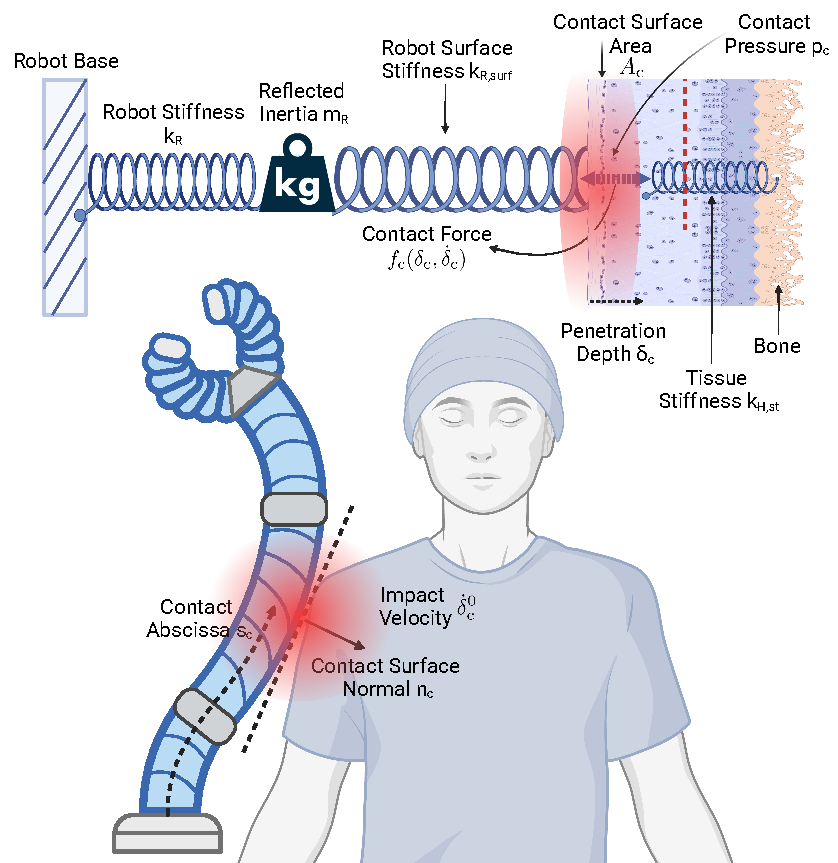
\includegraphics[width=0.65\linewidth]{safetymetric/figures/injury_severity_criterion.pdf}
    \caption{Proposed \glsxtrfull{SRISC} as a safety criterion for soft robots: The maximum contact pressure/stress $\max_t p_\mathrm{c}(t) = \max_t \frac{f_\mathrm{c}(t)}{A_\mathrm{c}}$ experienced during the (potential) collision acts as a proxy for the expected injury risk~\citep{iso2016collaborative}, where $f_\mathrm{c}(t)$ denotes the contact force and $A_\mathrm{c}$ the contact area. For computing $f_\mathrm{c}(t)$, we derive the dynamics of the collision (i.e., the time evolution of the penetration depth $\delta_\mathrm{c}(t)$) by projecting the dynamics of the soft robot onto a 1D Cartesian motion along the contact surface normal. In order to get a conservative estimate of the injury risk, we assume the human body part to be constrained in its motion (i.e., that the inertia of the human body part dominates the reflected inertia of the soft robot $m_\mathrm{R}$).}
    \label{fig:safetymetric:injury_severity_criterion_illustration}
\end{figure}

\subsection{Soft Robot Injury Severity Criterion}
Following the standards established in ISO/TS 15066:2016~\citep{iso2016collaborative}, we consider the maximum contact pressure, also sometimes referred to as stress~\citep{haddadin2009requirements}, experienced during the collision as a proxy for the injury risk. Therefore, we define the \gls{SRISC} for a given tuple $(q_{\mathrm{c}}^0,s_\mathrm{c}, n_\mathrm{c})$ capturing the contact geometry as
\begin{equation}
    \mathrm{SRISC}(q_{\mathrm{c}}^0,\dot{\delta}_\mathrm{c}^0,\tau,s_\mathrm{c},n_\mathrm{c}) = \max_t p_\mathrm{c} = \max_t \frac{f_\mathrm{c}(t)}{A_\mathrm{c}(t)} \leq \frac{\max_t f_\mathrm{c}(t)}{\min_t A_\mathrm{c}(t)} =  \frac{k_\mathrm{c} \max_t \delta_\mathrm{c}(t)}{\min_t A_\mathrm{c}(t)},
\end{equation}
where $p_\mathrm{c}(t)$ is the contact pressure/stress, and $A_\mathrm{c}$ is the contact area. We illustrate the derivation and definition of the \gls{SRISC} in Fig.~\ref{fig:safetymetric:injury_severity_criterion_illustration}.

The closed-form solution to the collision dynamics of \eqref{eq:safetymetric:collision_dynamics_cfs} allows us to upper-bound the maximum contact force $\max_t f_\mathrm{c}(t)$ that is encountered during the collision as
\begin{equation}\label{eq:safetymetric:maximum_contact_force_closed_form}
     \max_{t}f_\mathrm{c}(t) = k_\mathrm{c} \, \left ( \frac{f_\tau-f_{\mathcal{U}}^{\mathrm{c}0}}{k_\mathrm{R} + k_\mathrm{c}} + \sqrt{\left ( \delta_\mathrm{c}^0 - \frac{f_\tau-f_{\mathcal{U}}^{\mathrm{c}0}}{k_\mathrm{R} + k_\mathrm{c}} \right )^2 + \left (\dot{\delta}_\mathrm{c}^0 \right )^2 \frac{m_\mathrm{R}}{k_\mathrm{R} + k_\mathrm{c}} } \right ).
\end{equation}

\begin{figure}[ht]
    \centering
    \subfigure[Penetration depth $\delta_\mathrm{c}(t)$]{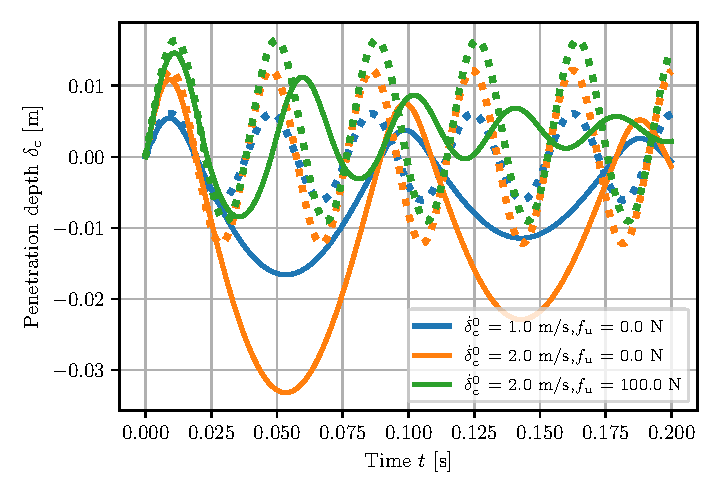
\includegraphics[width=0.49\linewidth, trim={5, 5, 5, 5}]{safetymetric/figures/closed_form_solution_verification/penetration_depth_vs_time.pdf}}
    \subfigure[Penetration velocity $\dot{\delta}_\mathrm{c}(t)$]{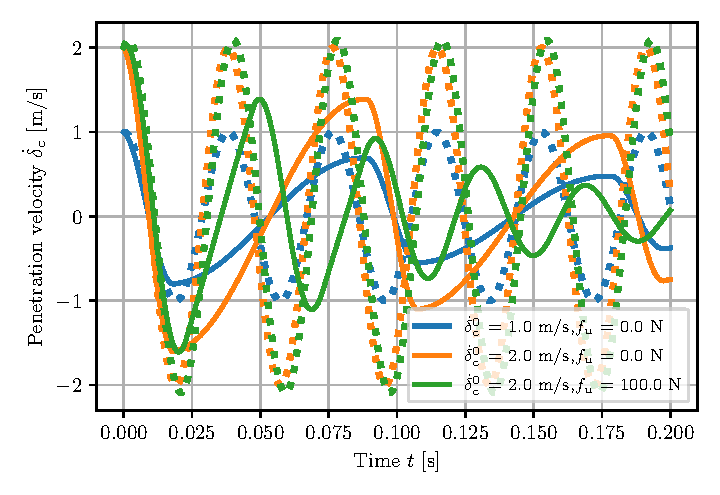
\includegraphics[width=0.49\linewidth, trim={5, 5, 5, 5}]{safetymetric/figures/closed_form_solution_verification/penetration_velocity_vs_time.pdf}}\\
    \subfigure[Contact force $f_\mathrm{c}(t)$]{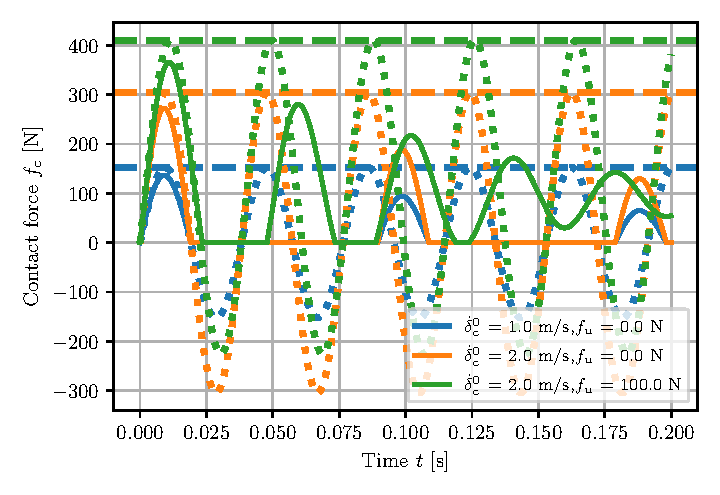
\includegraphics[width=0.5\linewidth, trim={5, 5, 5, 5}]{safetymetric/figures/closed_form_solution_verification/contact_force_vs_time.pdf}}
    \caption{
        Verification of closed-form solution to \eqref{eq:safetymetric:simplified_collision_dynamics}: The solid lines represent numerical integrations of the hybrid dynamics 
        $m_\mathrm{R} \, \Ddot{\delta}_\mathrm{c} + k_\mathrm{R} \, \delta_\mathrm{c} + d_\mathrm{R} \, \dot{\delta}_\mathrm{c} + f_\mathrm{c}(\delta_\mathrm{c}) = f_\tau - f_{\mathcal{U}}^{\mathrm{c}0}$ with $f_\mathrm{c}(\delta_\mathrm{c}) = k_\mathrm{c} \, \delta_\mathrm{c} + d_\mathrm{c} \, \dot{\delta}_\mathrm{c} \: \forall \, \delta_\mathrm{c} > 0$ and $f_\mathrm{c}(\delta_\mathrm{c}) = 0 \: \forall \; \delta_\mathrm{c} \leq 0$. 
        The dotted lines represent the closed-form solution to the time evolution reported in \eqref{eq:safetymetric:collision_dynamics_cfs} based on the dynamics in \eqref{eq:safetymetric:simplified_collision_dynamics} that describe the behavior during the contact phase. The dashed lines represent the (conservative) maximum contact force that could be encountered during the collision as determined by closed-form expression \eqref{eq:safetymetric:maximum_contact_force_closed_form}. 
        As system parameters, we choose $m_\mathrm{R} = \SI{1}{kg}$, $k_\mathrm{R} = \SI{2}{kN \per m}$, $d_\mathrm{R} = \SI{4}{Ns \per m}$, $k_\mathrm{c} = \SI{25}{kN \per m}$, which represents the spring constant of the human chest according to ISO/TS 15066:2016~\citep{iso2016collaborative}, $d_\mathrm{c} = \SI{20}{Ns \per m}$, and $\delta_\mathrm{c}^0 = \SI{0}{m}$.
        Please note that in all case we assume $f_{\mathcal{U}}^{\mathrm{c}0} = 0$ and $v_\mathrm{H} = 0$.
    }
    \label{fig:safetymetric:closed_form_solution_verification}
\end{figure}

We verify and visualize the behavior of the closed-form expression from \eqref{eq:safetymetric:collision_dynamics_cfs} and its upper bound \eqref{eq:safetymetric:maximum_contact_force_closed_form} in Fig.~\ref{fig:safetymetric:closed_form_solution_verification}. It can be clearly seen how \eqref{eq:safetymetric:maximum_contact_force_closed_form} represents a conservative upper bound on the actual contact forces the system experiences if we were to also account for the hybrid nature of the dynamics and the damping of the system.

\begin{figure}[ht!]
    \centering
    \subfigure[Initial deflection $q_\mathrm{c}^0$ vs. Robot stiffness $k_\mathrm{R}$]{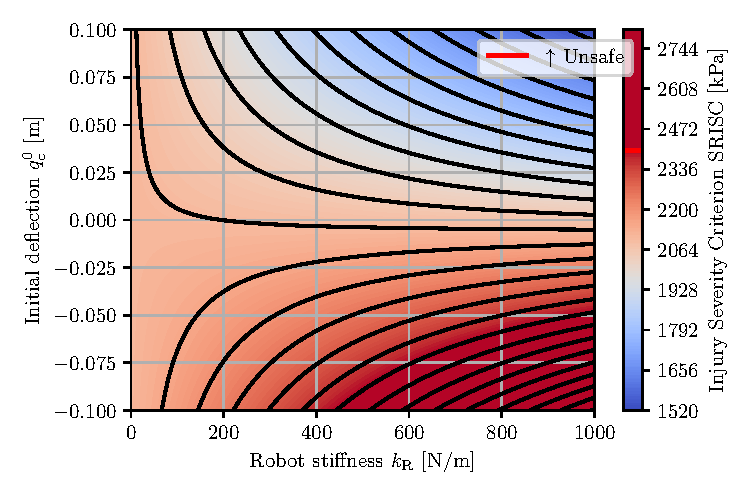
\includegraphics[width=0.49\linewidth, trim={5, 5, 5, 5}]{safetymetric/figures/mass_spring_robot/robot_stiffness_vs_initial_deflection.pdf}\label{fig:safetymetric:mass_spring_robot_characterization:robot_stiffness_vs_initial_deflection}}
    \subfigure[Contact stiffness $k_\mathrm{c}$ vs. robot stiffness $k_\mathrm{R}$]{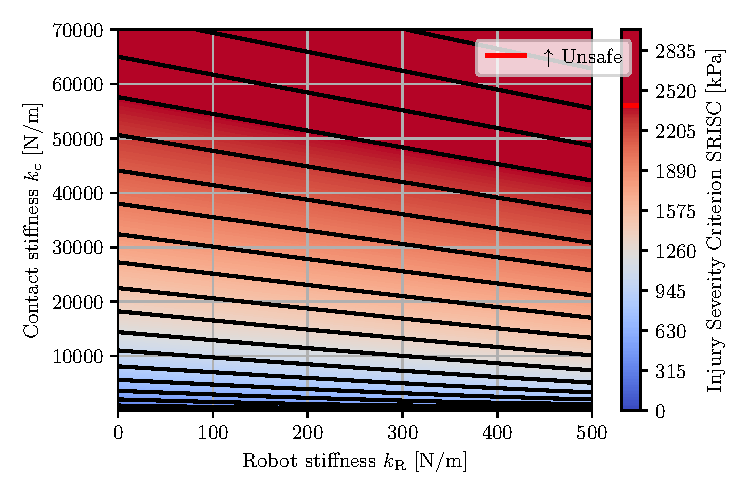
\includegraphics[width=0.49\linewidth, trim={5, 5, 5, 5}]{safetymetric/figures/mass_spring_robot/robot_stiffness_vs_contact_stiffness.pdf}\label{fig:safetymetric:mass_spring_robot_characterization:contact_stiffness_vs_robot_stiffness}}
    \\ \vspace{-0.2cm}
    \subfigure[Initial velocity $\dot{q}_\mathrm{c}^0$ vs. robot mass $m_\mathrm{R}$]{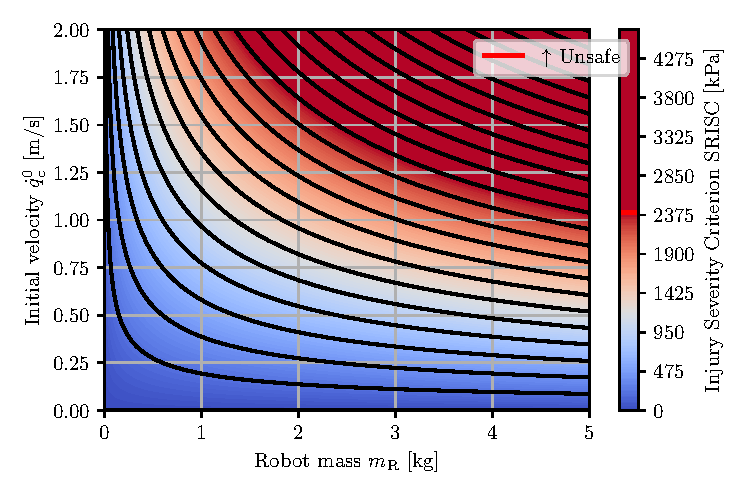
\includegraphics[width=0.49\linewidth, trim={5, 5, 5, 5}]{safetymetric/figures/mass_spring_robot/robot_mass_vs_initial_velocity.pdf}\label{fig:safetymetric:mass_spring_robot_characterization:robot_mass_vs_initial_velocity}}
    \vspace{-0.2cm}
    \caption{Characterization of the \gls{SRISC} on the mass-spring robot example.
        Here, we (closely) consider the collision between the mass-spring robot and the human chest. Therefore, if we conservatively assume the robot surface to be rigid, the spring constant of the contact with the chest is given as $k_\mathrm{c} = k_\mathrm{H} = \SI{25}{kN \per m}$. Furthermore, we assume a contact area of $\SI{1.5}{cm^2}$, an external force of $u=\SI{0}{N}$, and a equilibrium position of $q^0 = \SI{0}{m}$. Finally, according to ISO/TS 15066:2016~\citep{iso2016collaborative}, the maximum acceptable contact pressure/stress in transient conditions is given as $\SI{2400}{kPa}$, which serves as our threshold on the maximum acceptable \gls{SRISC}.
        \textbf{Panel~(a):} Evaluating the influence of robot stiffness $k_\mathrm{R}$ and the deflection of the soft robot at the beginning of the collision $q_\mathrm{c}^0$ on the \gls{SRISC}. We choose $m_\mathrm{R} = \SI{1}{kg}$ and $\dot{q}_\mathrm{c}^0 = \SI{2}{m/s}$.
        \textbf{Panel~(b):} Evaluating the influence of contact stiffness $k_\mathrm{c}$ and the robot stiffness $k_\mathrm{R}$ on the \gls{SRISC}. We choose $m_\mathrm{R} = \SI{1}{kg}$, $q_\mathrm{c}^0 = -\SI{0.1}{m}$, and $\dot{q}_\mathrm{c}^0 = -\SI{1.5}{m/s}$.
        \textbf{Panel~(c):} Evaluating the influence of robot mass $m_\mathrm{R}$ and the robot velocity at the beginning of the collision $\dot{q}_\mathrm{c}^0$ on the \gls{SRISC}. We choose $k_\mathrm{R} = \SI{1}{kN \per m}$ and $q_\mathrm{c}^0 = \SI{0}{m}$.
    }
    \label{fig:safetymetric:mass_spring_robot_characterization}
    \vspace{-0.2cm}
\end{figure}

\subsubsection{Example: Mass-Spring Robot}
First, we consider the most \emph{basic} soft robot - a damped mass-spring system with dynamics 
\begin{equation}
    m_\mathrm{R} \, \ddot{q} + k_\mathrm{R} \, (q-q^0) + d_\mathrm{R} \, \dot{q} = u + f_\mathrm{c},
\end{equation}
where $q \in \mathbb{R}$ and $q^0 \in \mathbb{R}$ is the equilibrium extension. 
Assuming $\delta_\mathrm{c}(t) = q(t)$ (i.e., the robot is in contact with the human when $q \geq 0$) and $v_\mathrm{H} = 0$, the \gls{SRISC} is then given by
\begin{equation}
     \mathrm{SRISC} = \frac{k_\mathrm{c}}{A_\mathrm{c}} \, \left (\frac{u - k_\mathrm{R} (q_{\mathrm{c}}^0 - q^0)}{k_\mathrm{R} + k_\mathrm{c}} + \sqrt{\left ( \frac{u - k_\mathrm{R} (q_{\mathrm{c}}^0 - q^0)}{k_\mathrm{R} + k_\mathrm{c}} \right )^2 + \left (\dot{q}_\mathrm{c}^0 \right )^2 \frac{m_\mathrm{R}}{k_\mathrm{R} + k_\mathrm{c}} } \right ),
\end{equation}
where $q_{\mathrm{c}}^0$ is the mass-spring position at which the collision starts and $\dot{q}_\mathrm{c}^0$ is the associated velocity.

Here, the \gls{SRISC} exhibits the limits
\begin{equation}
    \lim_{k_\mathrm{R} \to 0, u \to 0} \mathrm{SRISC} = \frac{\sqrt{m_\mathrm{R} \, k_\mathrm{c}}}{A_\mathrm{c}} \, \dot{q}_\mathrm{c}^0,
    \qquad
    \lim_{k_\mathrm{R} \to \infty} \mathrm{SRISC} = \frac{k_\mathrm{c}}{A_\mathrm{c}} \, \left ( - (q_{\mathrm{c}}^0 - q^0 ) + \left | q_{\mathrm{c}}^0 - q^0 \right | \right ).
\end{equation}
If $q_{\mathrm{c}}^0 \geq q^0$, which can be interpreted as the spring being in its equilibrium or stretched at the beginning of the collision, then the limit $k_\mathrm{R} \to \infty$ simplifies to $\lim_{k_\mathrm{R} \to \infty} \mathrm{SRISC} = 0$.

We characterize the \gls{SRISC} for this mass-spring robot example in the case of a collision with a human chest and present the results in Fig.~\ref{fig:safetymetric:mass_spring_robot_characterization}. 
Fig.~\ref{fig:safetymetric:mass_spring_robot_characterization:robot_stiffness_vs_initial_deflection} allows us to analyze what influence the robot stiffness has on the \gls{SRISC}: In the limit of $k_\mathrm{R} \to 0$ with $u = 0$, the contact pressure is solely influenced by the robot's initial velocity $\dot{q}_\mathrm{c}^0$, its mass $m_\mathrm{R}$, and the contact stiffness $k_\mathrm{c}$. However, as $k_\mathrm{R} > 0$, we can notice a bifurcation behavior: if the robot is stretched at the beginning of the collision (i.e., $q_\mathrm{c}^0 > 0$), then the contact stress \gls{SRISC} is decreased as $k_\mathrm{R}$ is increased. Oppositely, if the robot is compressed at the beginning of the collision (i.e., $q_\mathrm{c}^0 < 0$), then the contact stress \gls{SRISC} is increased as $k_\mathrm{R}$ is increased.
Fig.~\ref{fig:safetymetric:mass_spring_robot_characterization:contact_stiffness_vs_robot_stiffness} shows, as expected, that increasing the contact stiffness leads to a higher peak contact pressure.
Analog to the known results in the realm of rigid robotics~\citep{haddadin2009requirements, haddadin2013towards}, it can be easily seen in Fig.~\ref{fig:safetymetric:mass_spring_robot_characterization:robot_mass_vs_initial_velocity} how higher velocities and higher robot masses/inertia lead to higher injury severities and safety risks.
This analysis allows us to draw two important takeaways: (1) it is crucial to consider the maximum deformation of the soft robot we would expect to occur during operation to assess its safety, (2) as the robot's stiffness is increased, the \emph{worst-case} injury severity is also increased~\citep{abidi2017intrinsic} - confirming the intuition of how soft robots with their material softness and lower inertia exhibit a more compliant behavior than traditional rigid robots.

\begin{figure}[ht]
    \centering
    \subfigure[Contact backbone coordinate $s_\mathrm{c}$ vs. polar angle $\theta_\mathrm{c}$]{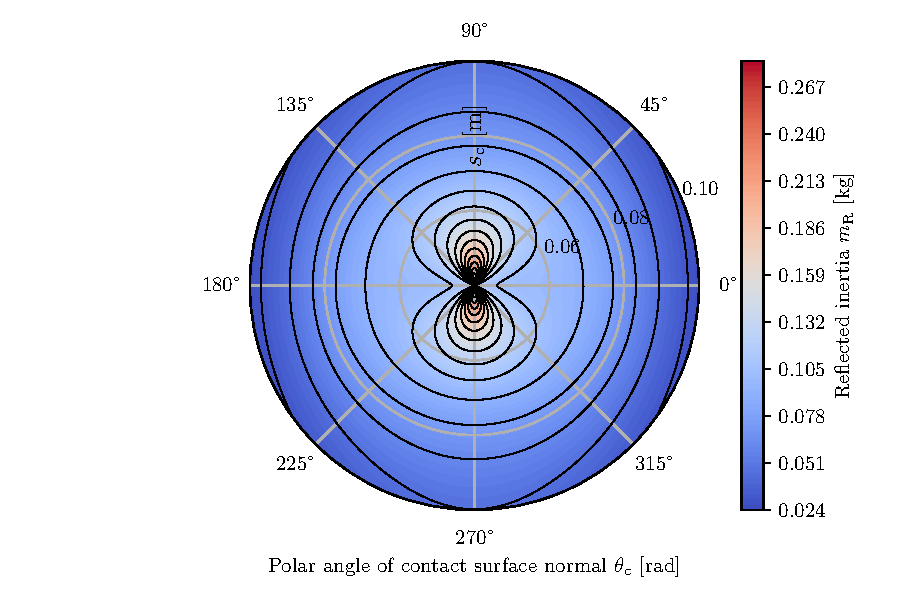
\includegraphics[width=0.43\linewidth, trim={5, 5, 5, 5}]{safetymetric/figures/planar_cs_reflected_inertia_characterization/planar_cs_reflected_inertia_for_theta_vs_s_c_cropped.pdf}}
    \subfigure[Bending strain $\kappa_\mathrm{be}$ vs. axial strain $\sigma_\mathrm{ax}$]{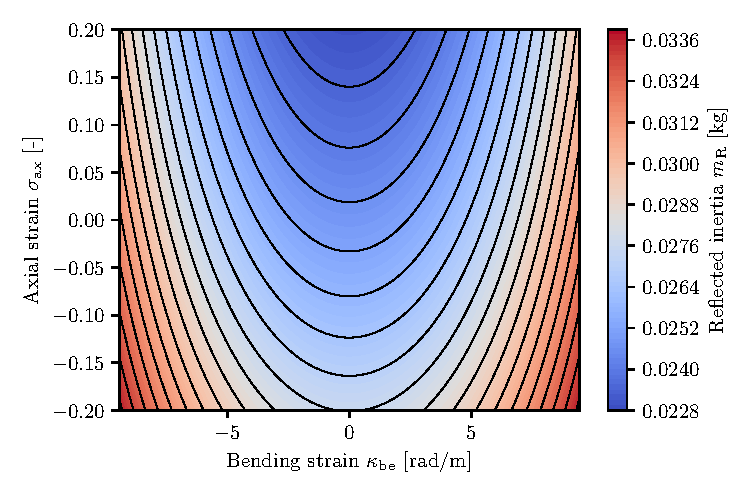
\includegraphics[width=0.56\linewidth, trim={5, 5, 5, 5}]{safetymetric/figures/planar_cs_reflected_inertia_characterization/planar_cs_reflected_inertia_for_kappa_be_vs_sigma_ax.pdf}}
    \caption{Characterization of the reflected inertia, also called effective mass~\citep{haddadin2009requirements, kirschner2021notion}, on the example of a planar \gls{CS} soft robot. 
    \textbf{Left:} Variation of the collision backbone coordinate $s_\mathrm{c}$ against the polar angle of contact $\theta_\mathrm{c}$, where $\theta_\mathrm{c} = 0$ corresponds to a perpendicular collision with the backbone and $n_\mathrm{c} = (1, 0)$ and $\theta_\mathrm{c} = \frac{\pi}{2}$ relates to a parallel collision with the robot backbone and $n_\mathrm{c} = (0,1)$. We assume here a soft robot in its equilibrium configuration (i.e., $q = 0_3$).
    \textbf{Right:} Variation of the bending strain $\kappa_\mathrm{be}$ and the axial strain $\sigma_\mathrm{ax}$ for a perpendicular collision ($n_\mathrm{c} = (0,1)$) at the distal end of the robot ($s_\mathrm{c} = \SI{0.1}{m}$).
    }
    \label{fig:safetymetric:planar_cs_reflected_inertia_characterization}
    \vspace{-0.2cm}
\end{figure}

\begin{figure}[ht]
    \centering
    \subfigure[Contact backbone coordinate $s_\mathrm{c}$ vs. polar angle $\theta_\mathrm{c}$]{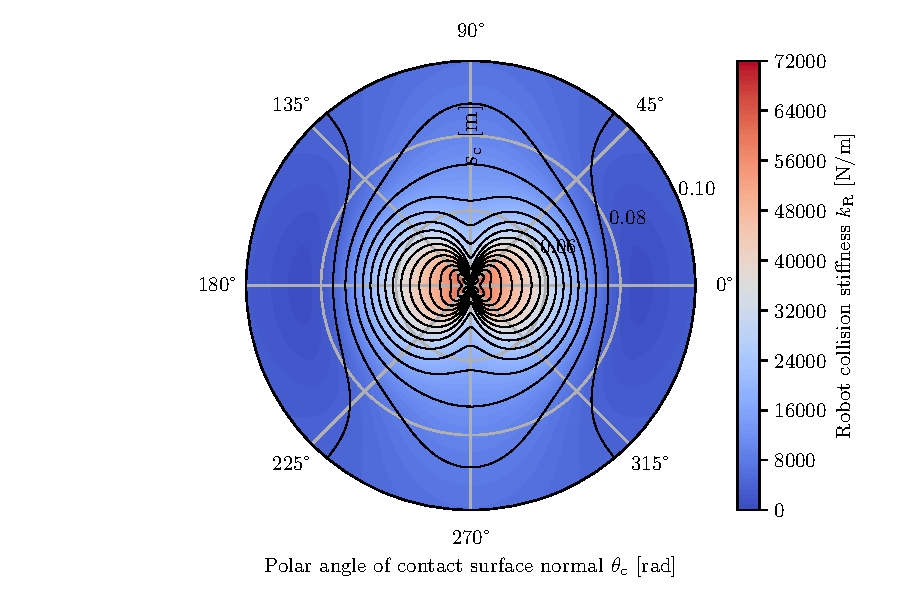
\includegraphics[width=0.49\linewidth]{safetymetric/figures/planar_cs_robot_collision_stiffness_characterization/planar_cs_robot_collision_stiffness_for_theta_c_vs_s_c_cropped.pdf}\label{fig:safetymetric:planar_cs_robot_collision_stiffness_characterization:theta_c_vs_s_c}}
    \subfigure[Bending strain $\kappa_\mathrm{be}$ vs. contact polar angle $\theta_\mathrm{c}$]{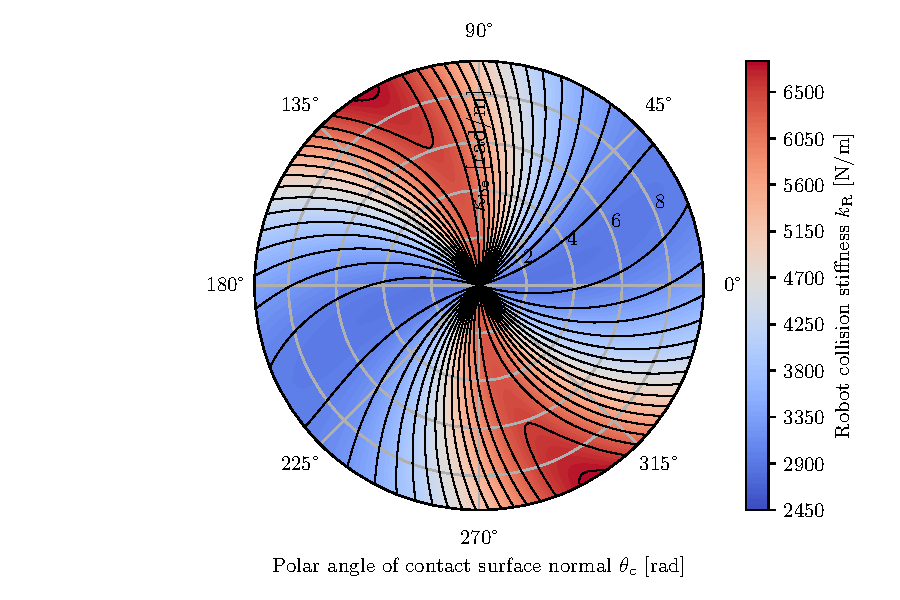
\includegraphics[width=0.49\linewidth]{safetymetric/figures/planar_cs_robot_collision_stiffness_characterization/planar_cs_robot_collision_stiffness_for_theta_c_vs_kappa_be_cropped.pdf}\label{fig:safetymetric:planar_cs_robot_collision_stiffness_characterization:theta_c_vs_kappa_be}}
    \caption{Characterization of the local robot collision stiffness $k_\mathrm{R}$ vs. polar angle $\theta_\mathrm{c}$ on the example of a planar \gls{CS} soft robot.
    \textbf{Left:} Variation of the collision backbone coordinate $s_\mathrm{c}$ against the polar angle of contact $\theta_\mathrm{c}$, where $\theta_\mathrm{c} = 0$ corresponds to a perpendicular collision with the backbone and $n_\mathrm{c} = (1, 0)$ and $\theta_\mathrm{c} = \frac{\pi}{2}$ relates to a parallel collision with the robot backbone and $n_\mathrm{c} = (0,1)$. We assume here a soft robot in its equilibrium configuration (i.e., $q = 0_3$).
    \textbf{Right:} Variation of the bending strain $\kappa_\mathrm{be}$ against the polar angle of contact $\theta_\mathrm{c}$ at the distal end of the robot ($s_\mathrm{c} = \SI{0.1}{m}$).
    }
    \label{fig:safetymetric:planar_cs_robot_collision_stiffness_characterization}
\end{figure}

\subsubsection{Example: Planar Piecewise Constant Strain Robot}
% 1 Figure giving an example how the contact location influences the injury severity.
% \begin{itemize}
%     \item Variation of injury severity for various contact geometries (e.g., various locations along the backbone, various contact surface normal) and configurations.
%     \item Variation across model discretization granularity.
% \end{itemize}

We now consider a planar $N$ segment \gls{PCS} robot, as introduced in Chapter~\ref{chp:background}. Here, the configuration of the $i$th segment is characterized by its spatially constant strain $\xi_i = \begin{bmatrix}
    \kappa_{\mathrm{be},i} & \sigma_{\mathrm{sh},i} & \sigma_{\mathrm{ax},i}
\end{bmatrix}^\top$, where $\kappa_{\mathrm{be},i}$ is the bending, $\sigma_{\mathrm{sh},i}$ the shear, and $\sigma_{\mathrm{ax},i}$ the axial/elongation strain~\citep{renda2018discrete}.
The collision dynamics are then given as
\begin{equation}
    \Lambda_\mathrm{c}(q) \, \Ddot{\delta}_\mathrm{c} + \eta_\mathrm{c}(q,\dot{q}) \, \dot{\delta}_\mathrm{c} + J_\mathrm{c,M}^{+\top}(q) ( G(q) + S \, q + D \dot{q} ) = J_\mathrm{c,M}^{+\top}(q) \, A(q) \, \tau - k_\mathrm{c} \, \delta_\mathrm{c} - d_\mathrm{c} \, \dot{\delta}_\mathrm{c},
\end{equation}
where $S \in \mathbb{R}^{3N \times 3N}$ is the linear stiffness of the robot, $G(q) \in \mathbb{R}^{3N}$ captures the gravitational forces, and $\tau \in \mathbb{R}^m$ represents the actuator forces.
We build the JAX~\citep{jax2018github} implementation of these dynamics on the \emph{JSRM}\footnote{\url{https://github.com/tud-phi/jax-soft-robot-modelling}} package~\citep{stolzle2024experimental}.

As we have seen in the previous example of the mass-spring robot, two of the variables that have the largest impact on the \gls{SRISC} are the reflected inertia $m_\mathrm{R}$, as defined in
\eqref{eq:safetymetric:constant_reflected_inertia_and_actuation_matrix_definition}, and the local soft robot stiffness in the collision direction $k_\mathrm{R}$, as defined in \eqref{eq:safetymetric:collision_potential_forces}.
Therefore, we present in Figures \ref{fig:safetymetric:planar_cs_reflected_inertia_characterization} \& \ref{fig:safetymetric:planar_cs_robot_collision_stiffness_characterization} a characterization of the reflected inertia $m_\mathrm{R}$ and the local robot stiffness $k_\mathrm{R}$, respectively.
In both cases, we consider a planar \gls{CS} segment (i.e., $N=1$) that has a length of $\SI{0.1}{m}$, a radius of \SI{0.02}{m}, a material density of \SI{1070}{kg \per m^3}, an elastic modulus of $E=\SI{0.5}{MPa}$ and a shear modulus of $G=\SI{0.2}{MPa}$.
The results show that the reflected inertia is highest at the proximal end of the robot/segment (i.e., $s_\mathrm{c} \to 0$) and for collisions that are parallel to the backbone, which, for our definition of our coordinate system with the soft robot in its straight configuration aligned with the y-axis, means that $\theta_\mathrm{c} = \frac{\pi}{2} + \pi \, n$ and $n_\mathrm{c} = \begin{bmatrix}
    0 & \pm 1
\end{bmatrix}^\top$. Furthermore, when considering perpendicular collisions with the backbone, the inertia increases with the bending strain and a compressed backbone (i.e., an increase in mass density).
Concerning the robot collision stiffness, we find that it is highest at the proximal end of the soft robot. At the distal end, we identify larger stiffnesses for parallel collisions, although the exact characteristics will depend on the choice of backbone radius/second moment of area. With increased bending strain, the polar angle with the highest stiffness will also change, as seen in Fig.~\ref{fig:safetymetric:planar_cs_robot_collision_stiffness_characterization:theta_c_vs_kappa_be}.

\begin{figure}[ht!]
    \centering
    \subfigure[Bending strain velocity $\dot{\kappa}_\mathrm{be}$ vs. mass density $\rho$]{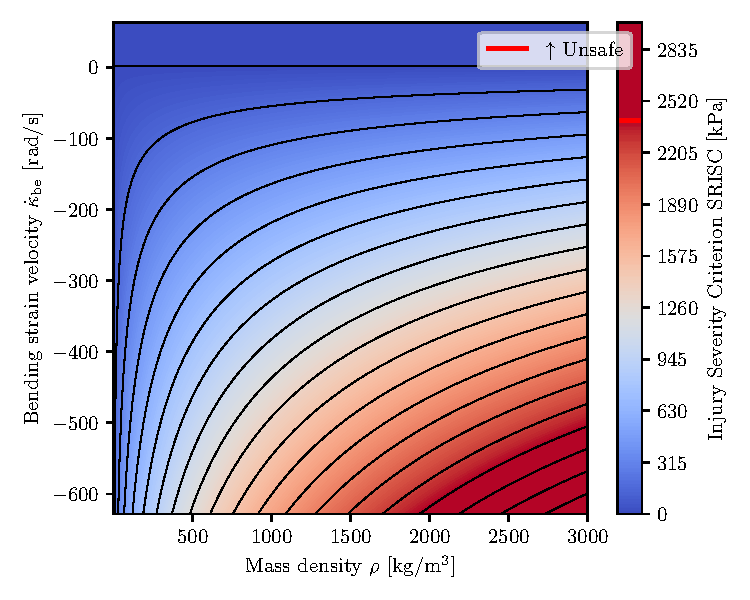
\includegraphics[width=0.49\linewidth]{safetymetric/figures/planar_cs_injury_severity_criterion/planar_cs_isc_for_bending_strain_velocity_vs_mass_density.pdf}\label{fig:safetymetric:planar_cs_injury_severity_criterion:bending_strain_velocity_vs_mass_density}}
    \subfigure[Robot length $L$ vs. backbone coordinate $s_\mathrm{c}$]{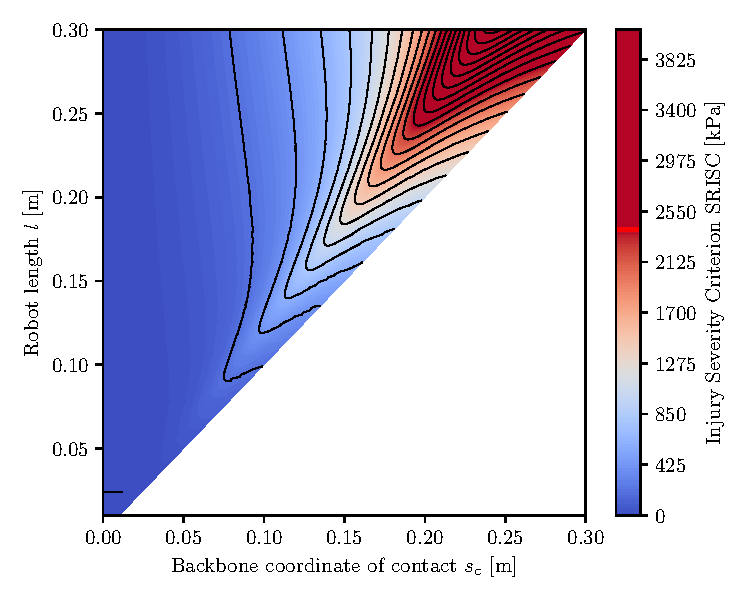
\includegraphics[width=0.49\linewidth]{safetymetric/figures/planar_cs_injury_severity_criterion/planar_cs_isc_robot_length_vs_s_c.pdf}\label{fig:safetymetric:planar_cs_injury_severity_criterion:robot_length_vs_s_c}}
    \\
    \subfigure[Contact backbone coordinate $s_\mathrm{c}$ vs. polar angle $\theta_\mathrm{c}$]{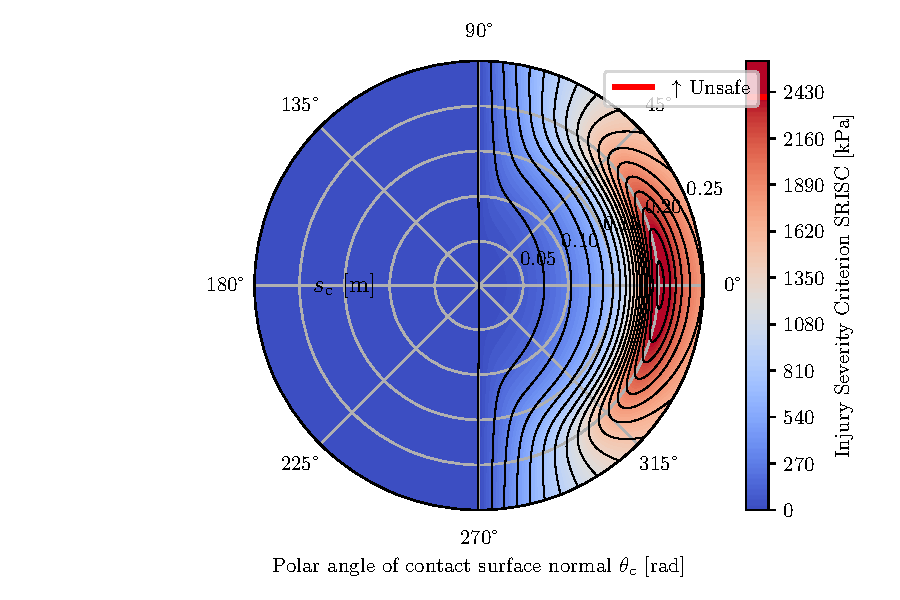
\includegraphics[width=0.49\linewidth]{safetymetric/figures/planar_cs_injury_severity_criterion/planar_cs_isc_for_theta_c_vs_s_c_cropped.pdf}\label{fig:safetymetric:planar_cs_injury_severity_criterion:theta_c_vs_s_c}}
    \subfigure[Bending strain $\kappa_\mathrm{be}$ vs. polar angle $\theta_\mathrm{c}$]{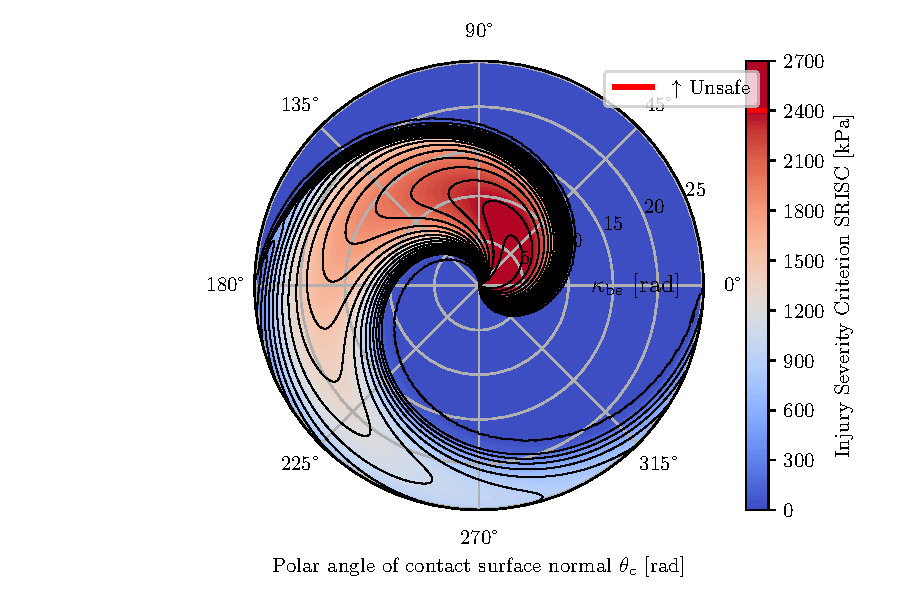
\includegraphics[width=0.49\linewidth]{safetymetric/figures/planar_cs_injury_severity_criterion/planar_cs_isc_for_theta_c_vs_kappa_be_cropped.pdf}\label{fig:safetymetric:planar_cs_injury_severity_criterion:theta_c_vs_kappa_be}}
    \caption{Characterization of the \gls{SRISC} on a planar \gls{CS} robot.
    \textbf{Panel~(a):} Variation of the robot's mass density $\rho$ and the bending strain velocity $\dot{\kappa}_\mathrm{be}$. We assume a perpendicular collision ($n_\mathrm{c} = (1,0)$) at the tip of the segment ($s_\mathrm{c} = \SI{0.25}{m}$).
    \textbf{Panel~(b):} Variation of the total robot length $L$ and the backbone coordinate $s_\mathrm{c}$ where the collision occurs. We assume a perpendicular collision ($n_\mathrm{c} = (1,0)$) with a soft robot in its equilibrium configuration (i.e., $q=0_3$).
    \textbf{Panel~(c):} Variation of the backbone coordinate $s_\mathrm{c}$ against the polar angle $\theta_\mathrm{c}$ of the contact surface where the collision occurs. Here, $\theta_\mathrm{c} = 0$ corresponds to a surface normal of $n_\mathrm{c} = (1,0)$ and $\theta_\mathrm{c} = \frac{\pi}{2}$ to $n_\mathrm{c} = (0,1)$. The soft robot is assumed to be in its equilibrium configuration (i.e., $q=0_3$).
    \textbf{Panel~(d):} Variation of the bending strain $\kappa_\mathrm{be}$ against the polar angle $\theta_\mathrm{c}$ of the contact surface where the collision occurs. We assume a collision with the distal end of the soft robot (i.e., $s_\mathrm{c} = \SI{0.25}{m}$).
    }
    \label{fig:safetymetric:planar_cs_injury_severity_criterion}
\end{figure}

In Fig.~\ref{fig:safetymetric:planar_cs_injury_severity_criterion}, we characterize the behavior of the \gls{SRISC} on the case of a planar \gls{CS} soft robot with a nominal robot length $L = \SI{0.25}{m}$, a backbone radius of $R = \SI{0.02}{m}$, a nominal mass density of $\rho = \SI{1070}{kg \per m^3}$, an elastic modulus of $E = \SI{0.5}{MPa}$, a shear modulus of $G = \SI{0.2}{MPa}$, a contact area of $A_\mathrm{c} = \SI{1.5}{cm^2}$, the spring constant of the human chest $k_\mathrm{H,st} = \SI{25}{kN \per m}$, and a soft robot surface material stiffness of $k_{\mathrm{R,surf}} = \SI{7.5}{kN \per m}$.
In all cases, we set the external forcing to $f_\tau = 0_3$, consider the human to be stationary and constrained with $v_\mathrm{H} = \SI{0}{m \per s}$, and assume a maximum threshold of \SI{2400}{kPa} on the \gls{SRISC}, which mirrors the maximum transient contact stress that is acceptable for collisions with the chest sternum according to ISO/TS 15066:2016~\citep{iso2016collaborative}.
% In Fig.~\ref{fig:safetymetric:planar_cs_injury_severity_criterion:bending_strain_velocity_vs_mass_density}, we can observe that, as expected, the maximum contact stress, and with that, the \gls{SRISC}, increases with mass density and a larger bending velocity in the direction of the collision.
% The results shown in Fig.~\ref{fig:safetymetric:planar_cs_injury_severity_criterion:robot_length_vs_s_c} are very interesting: while the \gls{SRISC} increases with an increased length of the segment, which is not too unexpected as longer soft robots exhibit larger Cartesian space velocities for the same strain-space velocities, we observe the the maximum contract stress is usually not at the tip of the distal end of the robot, but instead at at roughly \SI{75}{\percent} of its length. We hypothesize that the underlying reason is that some quantities, such as stiffness and reflected inertia, are at their maximum at the proximal end, while other quantities - in particular the Cartesian velocity - are at their maximum and the distal end leading the global maximum of the \gls{SRISC} to be in between proximal and distal end.
% Fig.~\ref{fig:safetymetric:planar_cs_injury_severity_criterion:theta_c_vs_s_c} exhibits the same characteristics while the polar angle with the maximum contact stress will always depend on the velocities and actuation that are applied to the soft robot.
% Finally, we observe in Fig.~\ref{fig:safetymetric:planar_cs_injury_severity_criterion:theta_c_vs_kappa_be} the maximum \gls{SRISC} to be at a straight backbone configuration with the \gls{SRISC} decreasing with an increased bending strain.
In Fig.\ref{fig:safetymetric:planar_cs_injury_severity_criterion:bending_strain_velocity_vs_mass_density}, we see that, as expected, the maximum contact stress—and therefore the \gls{SRISC}—rises with increased mass density and higher bending velocity in the collision direction. The results in Fig.~\ref{fig:safetymetric:planar_cs_injury_severity_criterion:robot_length_vs_s_c} are particularly intriguing: while the \gls{SRISC} increases with longer segment lengths—as longer soft robots exhibit higher Cartesian velocities for the same strain-space velocities—the maximum contact stress is typically not located at the very tip of the distal end but rather around \SI{75}{\percent} of the robot’s length. We hypothesize that this occurs because certain factors, such as stiffness and reflected inertia, peak at the proximal end, whereas others—especially Cartesian velocity—are maximized at the distal end, leading to an overall maximum \gls{SRISC} somewhere between the two. Similarly, Fig.~\ref{fig:safetymetric:planar_cs_injury_severity_criterion:theta_c_vs_s_c} displays analogous behavior, with the polar angle corresponding to the maximum contact stress varying based on the velocities and actuation applied to the soft robot. Finally, Fig.~\ref{fig:safetymetric:planar_cs_injury_severity_criterion:theta_c_vs_kappa_be} shows that the maximum \gls{SRISC} occurs at a straight backbone configuration, with the maximum \gls{SRISC} decreasing as bending strain increases.

\subsubsection{Example: Integrating a Control Policy}
% alternative heading: \subsection{Influence of Control Policy}
An important question when analyzing the safety of a closed-loop soft robotic system is what influence the control policy has on the \gls{SRISC}.
First, we consider a case where the behavior of the control policy $\tau(q,\dot{q})$ cannot be bounded or even inspected, such as it would be the case for controllers that contain integral terms or for many RL-based control policies.
In this case, access to actuation bounds $[\tau_\mathrm{min}, \tau_\mathrm{max}]$ provides us with the injury risk in the \emph{worst case scenario}.

Next, we consider the example of a \emph{PD+Feedforward}-like control structure that is relevant for many control policies that involve feedforward and/or feedback terms.
Specifically, we consider a fully-actuated setting (i.e., $n=m$) with an identity actuation matrix $A(q) = \mathbb{I}^n$.
Then, a regulator $\tau(q,\dot{q}) = \partial_{q} \, \mathcal{U}( q^\mathrm{d}) + K_\mathrm{p} \, (q^\mathrm{d}-q) - K_\mathrm{d} \, \dot{q}$ drives the system towards the setpoint $q^\mathrm{d}$~\citep{della2023model} and establishes the closed-loop dynamics
\begin{equation}
    M(q) \, \ddot{q} + C(q, \dot{q}) \, \dot{q} + \partial_{q} \, \mathcal{U}(q) + K_\mathrm{p} \, q + (D+K_\mathrm{d}) \, \dot{q} = \partial_{q} \, \mathcal{U}( q^\mathrm{d}) + K_\mathrm{p} \, q^\mathrm{d} + \tau_\mathrm{c},
\end{equation}
where $K_\mathrm{p}, K_\mathrm{d} \in \mathbb{R}^{n \times n}$ are the proportional and derivative feedback gains, respectively.
When re-formulating the simplified collision dynamics of \eqref{eq:safetymetric:simplified_collision_dynamics}, 
\begin{equation}
    m_\mathrm{R} \, \Ddot{\delta}_\mathrm{c} + (k_\mathrm{R} + k_\mathrm{c}) \, \delta_\mathrm{c} = J_\mathrm{c,M}^{+}(q_{\mathrm{c}}^0) \, (\partial_{q} \, \mathcal{U}(q^\mathrm{d}) +  K_\mathrm{p} \, q^\mathrm{d} - \partial_{q} \, \mathcal{U}(q_{\mathrm{c}}^0)).
\end{equation}
We notice that the feedforward control term acts through a constant force on the oscillatory system.
The proportional feedback term increases the local stiffness of the robot: $k_\mathrm{R} = \frac{\partial}{\partial q} J_\mathrm{c,M}^{+\top}(q) \, \left ( \partial_{q} \, \mathcal{U}(q) + K_\mathrm{p} \, q \right )\Big |_{q=q_{\mathrm{c}}^0} \,  J_\mathrm{c,M}^{+}(q_{\mathrm{c}}^0)$.
This analysis agrees with similar results known in literature~\citep{della2017controlling}.

\subsection{Soft Robot Design Hazardousness Criterion}
As presented in Fig.~\ref{fig:safetymetric:safety_metric_applications}, one application of a soft robotic safety metric would be to answer the question "\emph{How safe is this proposed soft robot design?}". The \gls{SRISC} on its own is not sufficient to answer this question as it relies on a knowledge of the soft robot state at the beginning of the collision $(q_{\mathrm{c}}^0, \dot{q}_{\mathrm{c}}^0)$, and the contact geometry $(s_\mathrm{c},n_\mathrm{c})$.
Therefore, we define the \gls{SRDHC} as the maximum injury severity that can be imposed by the soft robot over all feasible soft robot states, all possible contact geometries, and actuation sequences~\citep{wassink2007towards}
\begin{equation}
\begin{split}
    \mathrm{SRDHC} =& \: \max_{q \in \mathcal{Q}} \max_{\dot{\delta}_\mathrm{c}^0 \in [0,\dot{\delta}_\mathrm{c}^\mathrm{max}]} \max_{\tau \in [\tau_\mathrm{min}, \tau_\mathrm{max}]} \max_{s_\mathrm{c} \in (0,L]} \max_{n_\mathrm{c} \in \mathcal{S}^3} \mathrm{SRISC}(q_{\mathrm{c}}^0,\dot{\delta}_\mathrm{c}^0,\tau,s_\mathrm{c},n_\mathrm{c}),\\
    \leq& \: \max_{q \in \mathcal{Q}} \max_{s_\mathrm{c} \in (0,L]} \max_{n_\mathrm{c} \in \mathcal{S}^3} \mathrm{SRISC}(q_{\mathrm{c}}^0,\dot{\delta}_\mathrm{c}^\mathrm{max},\lVert \tau_\mathrm{max} \rVert_2,s_\mathrm{c},n_\mathrm{c}),
\end{split}
\end{equation}
where $\mathcal{Q}$ is the set of feasible soft robot configurations.
To make this optimization more tractable, we can leverage the stated upper bound with $\dot{\delta}_\mathrm{c}^\mathrm{max} = \lVert J_\mathrm{c} \rVert_2 \, \lVert \dot{q}_\mathrm{max} \rVert_2 + v_\mathrm{H}$
and $f_\tau^\mathrm{max} = \lVert A_\mathrm{c} \rVert_2 \, \lVert \max(|\tau_\mathrm{min}|,|\tau_\mathrm{max}|) \rVert_2$.
We note that the maximum value of $\dot{q}_\mathrm{max}$ that the robot can achieve autonomously is, in practice, often given by certain actuator characteristics (e.g., maximum servo velocity for tendon-driven actuation).

% We performed a preliminary investigation on the effect of the discretization on the estimated safety - and, in particular, the \gls{SRDHC}.
% The initial results reported in Fig.~\ref{fig:safetymetric:planar_pcs_design_hazardousness_criterion_discretization} show that approximating the soft robot with one or a few segments represents a conservative estimate of the actual safety - i.e., an overestimation of the injury severity. The underlying reason behind this behavior is that the actual soft robots can deform in infinite-dimensional space, while the approximation via the planar \gls{PCS} model limits the deformation modes and, with that, often increases the stiffness upon local contact. By increasing the discretization of the kinematic model underlying the safety metric, we can account for more deformation modes, and with that, reduce the overestimate of the injury severity.
We conducted a study to assess how discretization affects the estimated safety, with a particular focus on the \gls{SRDHC}. The initial results shown in Fig.~\ref{fig:safetymetric:planar_pcs_design_hazardousness_criterion_discretization} for varying the number of \gls{PCS} segments while keeping the robot length and all other system parameters constant indicate that approximating the soft robot with one or only a few segments leads to a conservative safety estimate—that is, an overestimation of the injury severity. This occurs because actual soft robots can deform in an infinite-dimensional space, whereas the planar \gls{PCS} model limits the available deformation modes and often increases the stiffness at the point of contact. By refining the discretization of the underlying kinematic model, we can capture more deformation modes and thereby reduce the overestimation of injury severity.

\begin{figure}
    \centering
    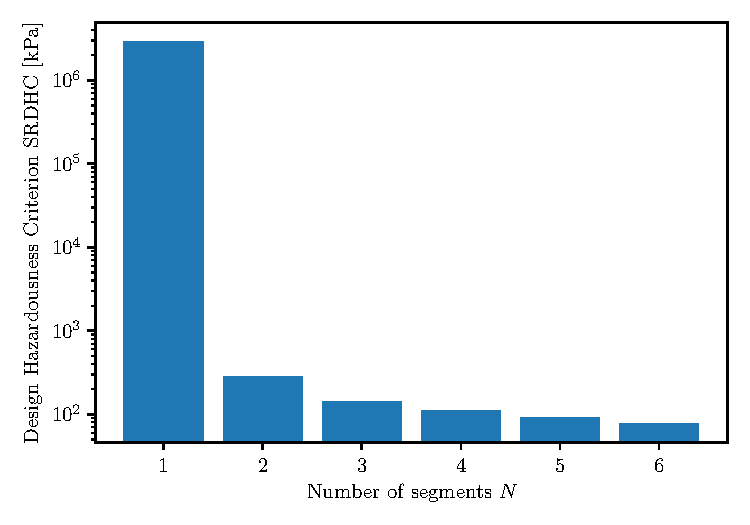
\includegraphics[width=0.5\linewidth]{safetymetric/figures/planar_pcs_design_hazardousness_criterion_discretization/design_hazardousness_criterion_bar_log.pdf}
    \caption{Analysis of the impact of varying the discretization of a planar \gls{PCS} robot on \gls{SRDHC} while keeping the total soft robot length constant at \SI{1}{m}.}
    \label{fig:safetymetric:planar_pcs_design_hazardousness_criterion_discretization}
\end{figure}
\section{Conclusion}
% In this chapter, we first highlighted the absence of a safety metric for soft robots, a gap that prevents the community from quantifying their safety advantages over rigid robot counterparts. This shortfall often results in designs that are ineffective in real-world tasks because they are excessively soft and lack sufficient payload capacity. We then discussed how a quantitative safety metric could be exploited in both design and control applications, ensuring safety without unduly compromising system performance by making the robot overly soft or the motion behavior overly cautious. Finally, we outlined the criteria such a safety metric must meet.
In this chapter, we first underscore the absence of a safety metric for soft robots—a gap that hinders the community from quantifying their safety benefits compared to rigid robots. This shortfall often leads to designs that perform poorly in real-world tasks because they tend to be overly soft and lack sufficient payload capacity. We then explored how a quantitative safety metric could be applied in both design and control contexts, ensuring safety without forcing the robot to be too soft or its motion overly cautious. Finally, we defined the criteria that such a safety metric must satisfy.

% Subsequently, we derived a quantitative safety metric for soft robots while considering the maximum contact pressure experienced during the collision, analog to the existing ISO norms for \glspl{Cobot}~\citep{iso2016collaborative}, as the safety criterion.
% For this the derivation of the safety metric, we rely on existing soft robot dynamic models, such as \gls{PCS}~\citep{renda2018discrete}\footnote{Please refer to Chapter~\ref{chp:background} for a discussion about alternative soft robot models that the safety metric could be based on.} and assume the human to be constrained, which represents the \emph{worst case}~\citep{haddadin2009requirements}.
% The proposed safety metric comes into two flavors: the \gls{SRISC} can be evaluated in closed-form and determines the maximum contact pressure experienced during a soft robot - human collision for a given initial condition, consting of soft robot configuration, velocity and contact geometry, and a given constant (e.g., worst-case) actuation. The \gls{SRISC} is in particular suitable for \emph{safety-aware control} applications.
% However, when designing soft robots, we need to ensure safety within a given operating envelope consisting of infinitely many initial conditions. For this case, we developed the \gls{SRDHC} which determines the maximum \gls{SRISC} for a given specification of operating conditions (e.g., maximum deformation, actuator bounds, configuration-space velocities), in particular across all possible contact geometries.
Next, we derived a quantitative safety metric for soft robots by considering the maximum contact pressure during a collision, analogous to the existing ISO norms for \glspl{Cobot}~\citep{iso2016collaborative}, as our safety criterion. For the derivation, we relied on established soft robot dynamic models, such as \gls{PCS}~\citep{renda2018discrete}\footnote{Please refer to Chapter~\ref{chp:background} for a discussion of alternative soft robot models that could serve as the basis for the safety metric.}, and assumed a constrained human model to represent the \emph{worst case} scenario~\citep{haddadin2009requirements}. The proposed safety metric is offered in two forms: the \gls{SRISC}, which can be computed in closed-form and estimates the maximum contact pressure during a soft robot–human collision given a specific initial condition—comprising the robot’s configuration, velocity, contact geometry, and a predetermined (e.g., worst-case) actuation—and is particularly well-suited for \emph{safety-aware control} applications. In contrast, when designing soft robots, it is necessary to guarantee safety across an operating envelope that encompasses infinitely many initial conditions. For this purpose, we developed the \gls{SRDHC}, which determines the maximum \gls{SRISC} for a given set of operating conditions (e.g., maximum deformation, actuator bounds, configuration-space velocities), especially considering all potential contact geometries.

% Crucially, the proposed safety metric meets all (compulsory) requirements specified in Sec.~\ref{sub:safetymetric:safety_metric_requirements}, as it, for example, accounts for collisions along the entire soft robot body, the assumptions and simplifications taken during the derivation lead to a conservative estimate of the true safety, the computation of the safety metric is tractable as (a) we do not need to the collision dynamics in time but rather have access to the maximum contact force in closed form, (b) part of the computation can be vectorized/parallelized. Furthermore, the safety metric is differentiable - even analytically as our implementation in JAX~\citep{jax2018github} provides gradients via autodifferentiation.
Notably, the proposed safety metric fulfills all mandatory requirements outlined in Sec.~\ref{sub:safetymetric:safety_metric_requirements}. For instance, it takes into account collisions along the entire soft robot body, and the assumptions and simplifications made during its derivation result in a conservative estimate of true safety. Additionally, the metric is computationally tractable because (a) it bypasses the need to simulate collision dynamics over time by providing the maximum contact pressure in closed form, and (b) portions of the computation can be vectorized or parallelized. Moreover, the metric is differentiable—even analytically—since our implementation in JAX~\citep{jax2018github} offers gradients through autodifferentiation.

% Notably, the characterization of the proposed safety metric demonstrated, that the safety of soft robots is not solely determined by material softness, but that instead, also their mass density, actuation, control and operating conditions (e.g., velocity, maximal deformation) play a significant role.
% In particular, feedback gains increase the stiffness of closed-loop system~\cite{della2017controlling, della2023model} therefore also for soft robots, the safety is decreased.
% Furthermore, counter usual intuition, the maximum injury severity is caused neither by collisions at the proximal or distal end, but instead somewhere in between.
% Finally, preliminary research shows that the numerous \glspl{DOF} that soft robot exhibit could be playing a significant role in distributing the contact energy and reducing the maximum local contact pressure.
Notably, the characterization of the proposed safety metric demonstrates that the safety of soft robots is determined not only by their material softness but also by factors such as mass density, actuation, control, and operating conditions (e.g., velocity, maximum deformation). In particular, increased feedback gains raise the stiffness of the closed-loop system~\citep{della2017controlling, della2023model}, thereby reducing safety even for soft robots. Moreover, contrary to common intuition, the maximum injury severity does not occur at either the proximal or distal end, but rather somewhere in between. Finally, preliminary research suggests that the numerous degrees of freedom (\glspl{DOF}) in soft robots may play a significant role in distributing contact energy and reducing the maximum local contact pressure.

% For future work, two critical aspects then emerge: (1) experimentally validating the safety criterion—i.e., measuring the discrepancy between the predicted and actual safety criterion—and (2) establishing appropriate thresholds~\citep{iso2016collaborative, behrens2022statistical} for the safety criterion (i.e., acceptable injury risk) to ensure safety in human-centric environments. Here, analog the existing literature on rigid robots~\citep{yamada1997evaluation, muttray2014collaborative, behrens2022statistical}, empirical biomechanical studies could play a crucial role in this process.
% It is important to note that safety requirements may differ significantly depending on the specific robotic application and task. For instance, a soft robot designed as a children's toy must adhere to much stricter safety standards than one used for industrial refueling. Understanding such varying requirements is crucial to ensuring safe and effective performance. 
Looking ahead, two key aspects emerge for future work: (1) the experimental validation of the safety criterion—i.e., quantifying the discrepancy between predicted and actual safety—and (2) the establishment of appropriate thresholds~\citep{iso2016collaborative, behrens2022statistical} for the safety criterion (in terms of acceptable injury risk) to ensure safety in human-centric environments. Drawing inspiration from existing literature on rigid robots~\citep{yamada1997evaluation, muttray2014collaborative, behrens2022statistical}, empirical biomechanical studies could play a crucial role in this process. It is also essential to recognize that safety requirements may vary considerably depending on the specific robotic application and task. For example, a soft robot designed as a children’s toy must comply with much stricter safety standards than one intended for industrial refueling. Understanding these differences is key to achieving safe and effective performance.

% Furthermore, the safety metric itself can be extended and improved. For example, specializing in safety metrics for different soft robot modeling techniques, such as FEM-based and geometric strain-based approaches, will enable more accurate risk assessments tailored to specific designs. Extending these metrics to closed-chain robots, locomotors, and wearable systems will further solidify safety evaluation frameworks across diverse robotic applications.
Furthermore, the safety metric itself can be extended and refined. By developing specialized metrics tailored to different soft robot modeling techniques—such as \gls{FEM}- or \gls{GVS}-based approaches—more accurate risk assessments can be achieved for specific designs. Extending these metrics to closed-chain robots, locomotors, and wearable systems will further strengthen safety evaluation frameworks across a diverse range of robotic applications.

% Finally moving to applications, we find it crucial to develop develop design and control concepts that can exploit the proposed safety metric.
% First considering \emph{safety-aware design}, a critical next step involves identifying which design parameters most significantly affect safety in different types of actuation, such as tendon-driven and pneumatically actuated soft robots. Mapping out these dependencies will provide actionable insights for designers seeking to enhance safety.
% Furthermore, we propose in Appendix~\ref{chp:apx:holisticcodesign} a strategy for co-optimizing the safety of soft robots via co-design~\citep{zardini2023co, spielberg2019learning, wang2024diffusebot, navez2024contributions}, which will allow to explicitly formalize and quantify the tradeoff between safety and performance in soft robotics.
Finally, with regard to practical applications, it is vital to develop design and control strategies that take full advantage of the proposed safety metric. In the context of\emph{safety-aware design}, a crucial next step is to identify which design parameters most significantly impact safety for various actuation types, such as tendon-driven versus pneumatically actuated soft robots. Mapping these dependencies will provide designers with actionable insights to enhance safety. Additionally, as outlined in Appendix~\ref{chp:apx:holisticcodesign}, we propose a holistic co-design strategy for optimizing the safety of soft robots~\citep{zardini2023co, spielberg2019learning, wang2024diffusebot, navez2024contributions}, which will enable the explicit formalization and quantification of the trade-off between safety and performance in soft robotics.
% On the other hand, \emph{safety-aware control} could be achieved via \gls{MPC} or \glspl{CBF}~\citep{ames2016control, ferraguti2020control}, which would enable us to push the performance (e.g., speed~\citep{haggerty2023control}) as much as possible while still guaranteeing safety in all scenarios.
Additionally, \emph{safety-aware control} can be implemented, for example, using \gls{MPC} or \glspl{CBF}~\citep{ames2016control, ferraguti2020control}, enabling us to maximize performance, such as the motion speed~\citep{haggerty2023control}, while ensuring safety in all scenarios.

% \section{Design of Safe Soft Robots}
% \begin{itemize}
%     \item Based on the insights gained in Section~\ref{sec:safety_metric}, give \emph{simple} insights how safe designs can be achieved.
%     \item Stiffness of the soft robot design (i.e., not just of the material) should be reduced, particularly close to the base/proximal end.
%     \item Reflected mass (e.g., material density \& volume) should be reduced, in particular close to the tip/distal end.
%     \item Guidelines for establishing safe controllers.
%     \item Specifically, explain how the combination of robot stiffness and the proportional control gains impacts the design hazardousness.
%     \item However, we stress that \emph{simple} guidelines that guarantee a specific safety level cannot be (easily) expressed. Therefore, we require a co-design methodology that takes into account the safety metric.
% \end{itemize}



\part{Shape Sensing and Control with Advanced Physics-based Models}\label{part:physicsmodels}
% \chapter{Sensing Soft Robots' Shape with Cameras: An Investigation on Kinematics-Aware SLAM}
\chapter{Shape Sensing with Cameras: An Investigation on Kinematics-Aware SLAM}
\label{chp:srslam}

\begin{foreword}
    Before we can develop advanced soft robot controllers, we require access to state information. Specifically, we need to know the configuration of the soft robot, which, as introduced in Chapter~\ref{chp:background}, is for soft robots usually defined as the parametrized shape of the backbone.
    In this chapter, we demonstrate how we can augment in a plug-and-play fashion existing state-of-the-art \gls{SLAM} algorithms with kinematic knowledge to achieve shape sensing for soft robots.
\end{foreword}

\begin{abstract}
    % The nature of continuum soft robots calls for novel perception solutions, which can provide information on the robot's shape while not substantially modifying their bodies' softness. One way to achieve this goal is to develop innovative and completely deformable sensors. 
    One way to achieve proprioception of the soft robot's shape while not substantially modifying their bodies' softness is to develop innovative and completely deformable sensors. 
    However, these solutions tend to be less reliable than classic sensors for rigid robots. As an alternative, we consider here the use of monocular cameras. By admitting a small rigid component in our design, we can leverage well-established solutions from mobile robotics. We propose a shape-sensing strategy that combines a SLAM algorithm with nonlinear optimization based on the robot's kinematic model. We prove the method's effectiveness in simulation and with experiments of a single-segment continuous soft robot with a camera mounted to the tip. We achieve mean relative translational errors below 9\% simulations and experiments alike and as low as 0.5\% on average for some simulation conditions.
\end{abstract}

\blfootnote{
    This chapter is partly based on \faFileTextO~\emph{E. Rosi*, \textbf{M. Stölzle}*, F. Solari, and C. Della Santina (2022, April). Sensing Soft Robots' Shape with Cameras: an Investigation on Kinematics-Aware SLAM. In 2022 IEEE 5th International Conference on Soft Robotics (RoboSoft) (pp. 795-801). IEEE.}~\citep{rosi2022sensing}.

    % \nth{1}-author contributions: E. Rosi implemented the methodology, collected the simulation results, and executed the lab experiments with a soft segment. M. Stölzle provided guidance on the methodology, helped debug the implementation of the approach in code, contributed to the experimental setup (e.g., motion capture system, fabrication of the soft segment), and wrote the paper.

    C.D.S. conceived and led the project.
    E.R. implemented the methodology, collected the simulation results, and executed the lab experiments with a soft segment.
    M.S. contributed ideas to the methodology, helped debug the implementation of the approach in code, contributed to the experimental setup (e.g., motion capture system, fabrication of the soft segment), and wrote the paper.
    C.D.S., E.R., and M.S. revised the manuscript.
    C.D.S, F.S., and M.S. supervised the research project.
    C.D.S. provided funding.
}


%% Start the actual chapter on a new page.
\newpage

\section{Introduction}\label{sec:srslam:introduction}
%
With their bodies entirely made of soft deformable materials, continuum soft robots are especially suited for application domains involving safe and robust interaction with humans and environment, and ranging from inspection, to healthcare and agriculture~\cite{majidi2014soft,elfferich2021soft}. To achieve these goals, soft robots must first master the art of controlling and sensing their body shape in space \cite{della2023model}.
%
% We refer to the estimation of the robot shape uniquely from on-board sensors as propriocetive shape sensing.
%
% Methods widely used in rigid robotics are not always applicable to soft systems, and what can be achieved in a simple way for rigid bodies may not be such for soft ones. One relevant example is the 
% ... challenge of sensing the robot's configuration, which in rigid robots can be achieved with well established technologies as encoders placed at the joint. 
%
A major challenge with shape perception in soft robots is that sensing strategies must not compromise the intrinsic softness of these systems~\cite{polygerinos2017soft,wang2018toward}. %In the literature they mainly propose resistive, capacitive and magnetic sensors to achieve proprioception \cite{cianchetti2012sensorization,polygerinos2017soft,atalay2017batch,atalay2018highly}.
%
% One way to achieve this goal is to look for . 
To this end, researchers have proposed several entirely deformable sensors over the years, including capacitive~\cite{scimeca2019model},  and optical sensors~\cite{li2021scaling}, liquid metal~\cite{wall2017method}. These solutions are quite attractive since they minimally corrupt the physical softness of the robot. However, they usually require complex learning strategies to be used since their behavior is hard to model~\cite{thuruthel2019soft,truby2020distributed}.
%
% wall an brock sousace finger
% moritz otpmized sensing

An alternative is to relax the constraint of complete deformability and allow from small rigid components. This strategy enables rethinking the use of existing sensing technologies in this radically new context. Examples are hall sensors~\cite{guo2019continuum}, IMUs~\cite{hughes2020sensing}, and microphones~\cite{zoller2018acoustic}. %wall and brock
%
The information gathered from inward-facing cameras looking at features in soft chambers' inner walls has proven sufficient to estimate the configuration~\cite{she2020exoskeleton,werner2020vision}, and characterize contacts with the environment \cite{ward2018tactip,lin2020curvature}. However, all these strategies need machine learning to transform the image information in the desired physical quantity.
%
%Classical image filters for feature extraction are combined with \gls{SVR} to estimate a tip position from the camera images. % Their approach performs similarly to a performance baseline made with an off-the-shelf distance sensor used to measure the linear extension.
%
% Another research by Wongwilai et al.~\cite{wongwilai2014slam} proposes a framework that combines all grasping tasks (object model acquisition, grasping point calculation and navigation of the robotic arm) with a RGB-D \gls{SLAM}.
%
% In contrast, fewer papers explore the use of camera images for proprioception. Weber et al.~\cite{weber2012multi} use an array of micro-cameras which face the environment to estimate the configuration of a single segment robot. The algorithm employs a configuration estimation refinement followed by a full \gls{BA}. 
%
%Cheng et al.~\cite{cheng2020approximate} present a kinematic equivalent model for a planar continuum robot. They build an Approximate \gls{PCC} model, using classical rigid linkages (2L-5R). They also propose a configuration estimation of the planar continuum robot using a monocular camera as an application to their model.
%
%\textbf{\cite{wang2018robot}} they combine SLAM and manipulation for a humanoid robot (Atlas).
%
%\textbf{\cite{klingensmith2016articulated}} they use RGB-D SLAM for estimating joint angles of an articulated manipulator. 
%
%\textbf{\cite{wongwilai2014slam}} they use SLAM for grasping (depth camera). they combine the process of data acquisition, navigation and grasp point calculation together.
%
Alternatively, cameras mounted outwards on the robot's tip and have been used to execute visual servoing~\cite{homberg2019robust}.
% more citations: wang2013visual
%
In the best of Authors' knowledge, the only two works dealing with continuum (non-soft) robots are \cite{weber2012multi} and \cite{cheng2020approximate}.
% 
The first uses \gls{BA} to integrate the output of multiple cameras embedded in a single segment. The second uses hand-tuned features to estimate the robot configuration within a novel kinematic model. Thus, no general strategy to estimate the whole state of a soft segment from a single monocular camera exists in the literature.

\gls{SLAM} is one of the most effective and largely used strategies for vision-based localization for mobile robots and autonomous vehicles~\cite{fuentes2015visual,mur2017orb}. %SLAM has been used been widely used in autonomous vehicles \cite{x} and rigid robots~\cite{klingensmith2016articulated}.
%
In this work, we investigate using monocular \gls{SLAM} to estimate the location of selected points across the soft robot. We then propose a mechanism for simultaneously refining the estimation and reconstructing the complete shape of the robot. We do that by retracting the output of the \gls{SLAM} to the manifold of camera configurations admitted by the kinematic model of the soft robot. We formulate this action as a nonlinear optimization problem. Fig.~\ref{fig:srslam:method_overview} summarizes the proposed architecture. We test the strategy with simulations and experiments, achieving mean relative translational errors between \SI{0.4}{\percent} and \SI{9}{\percent} in the former, and from \SI{5}{\percent} to \SI{9}{\percent} in the latter.

\begin{figure*}[ht]
     \centering
     \subfigure[Overview]{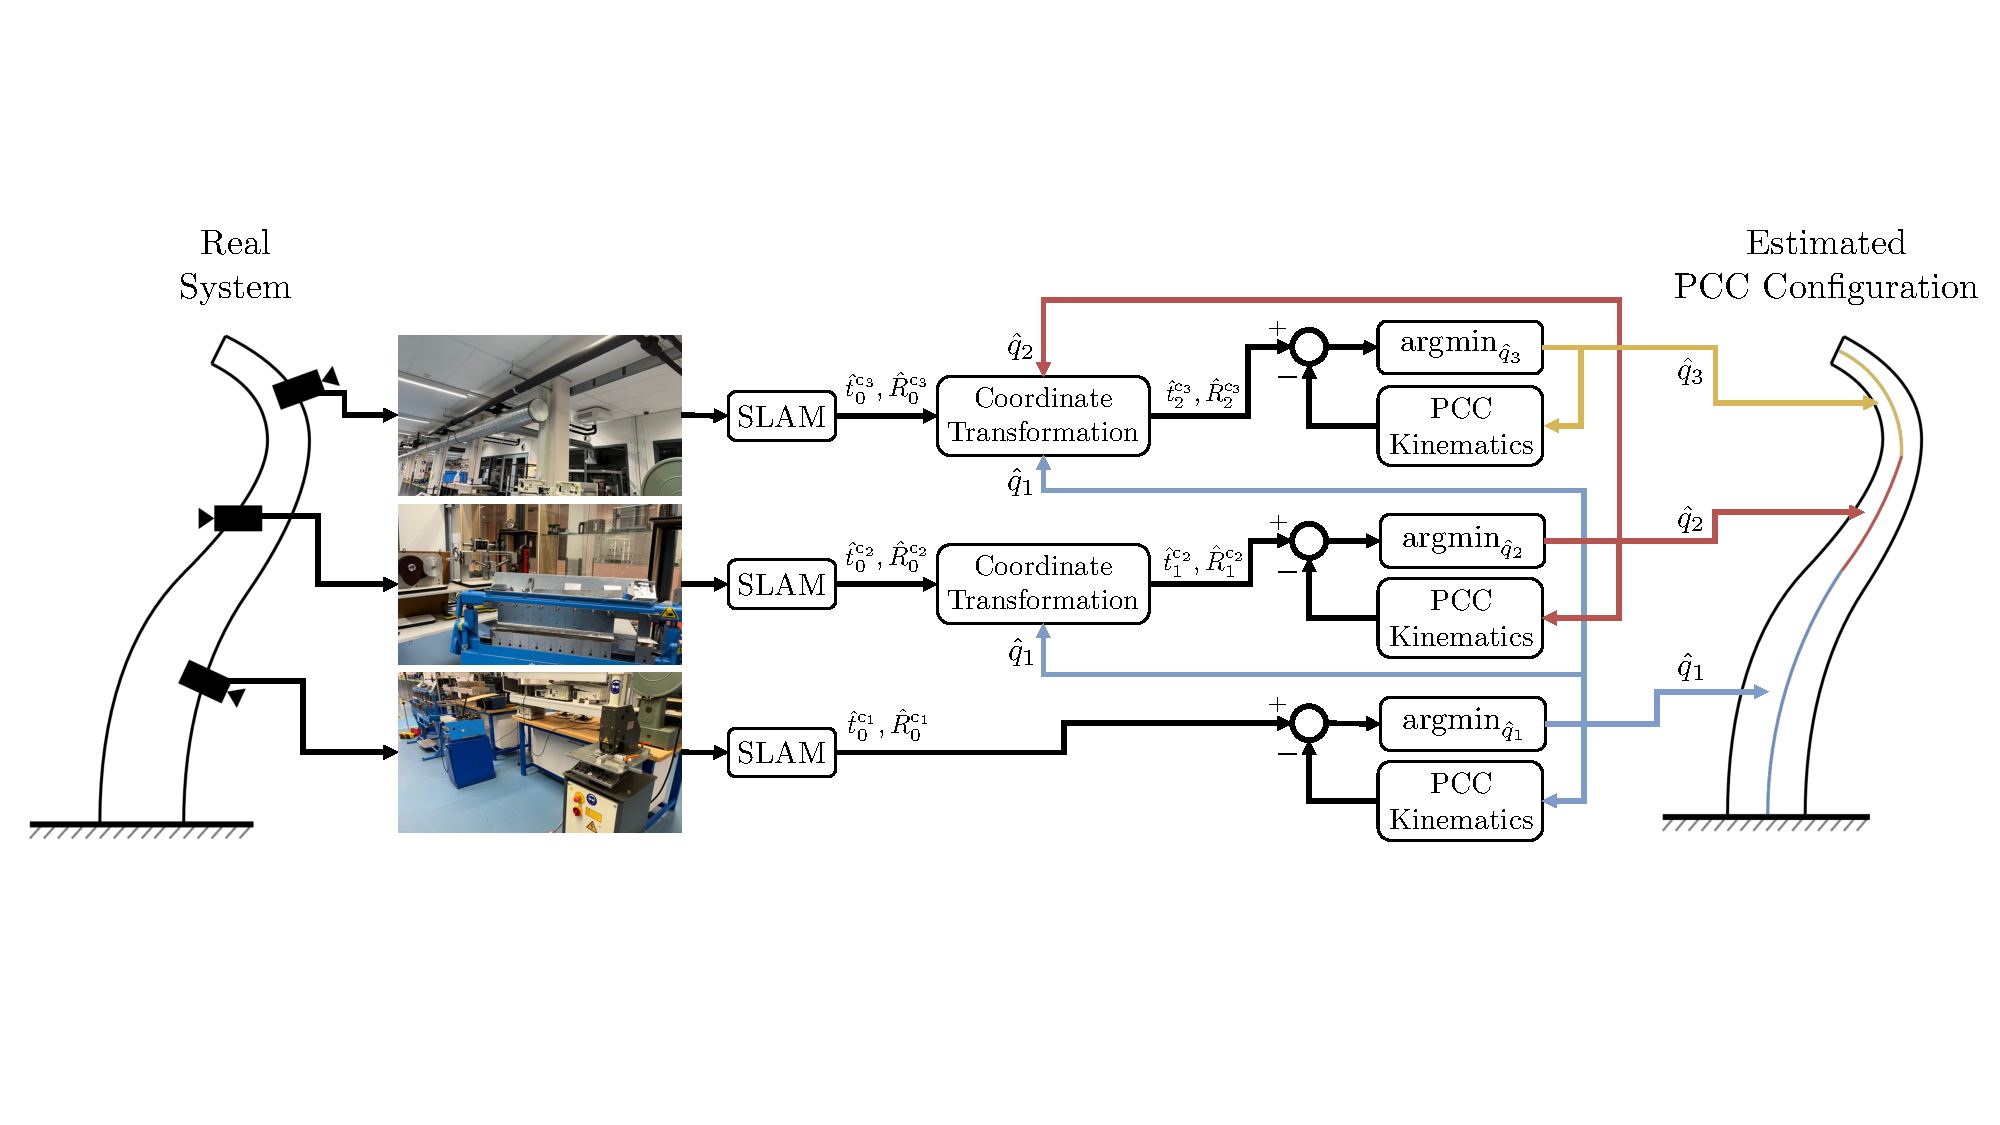
\includegraphics[width=0.69\columnwidth]{srslam/figures/graphic_method_overview_v5_cropped.pdf} \label{fig:srslam:method_overview}}
     \subfigure[Kinematics]{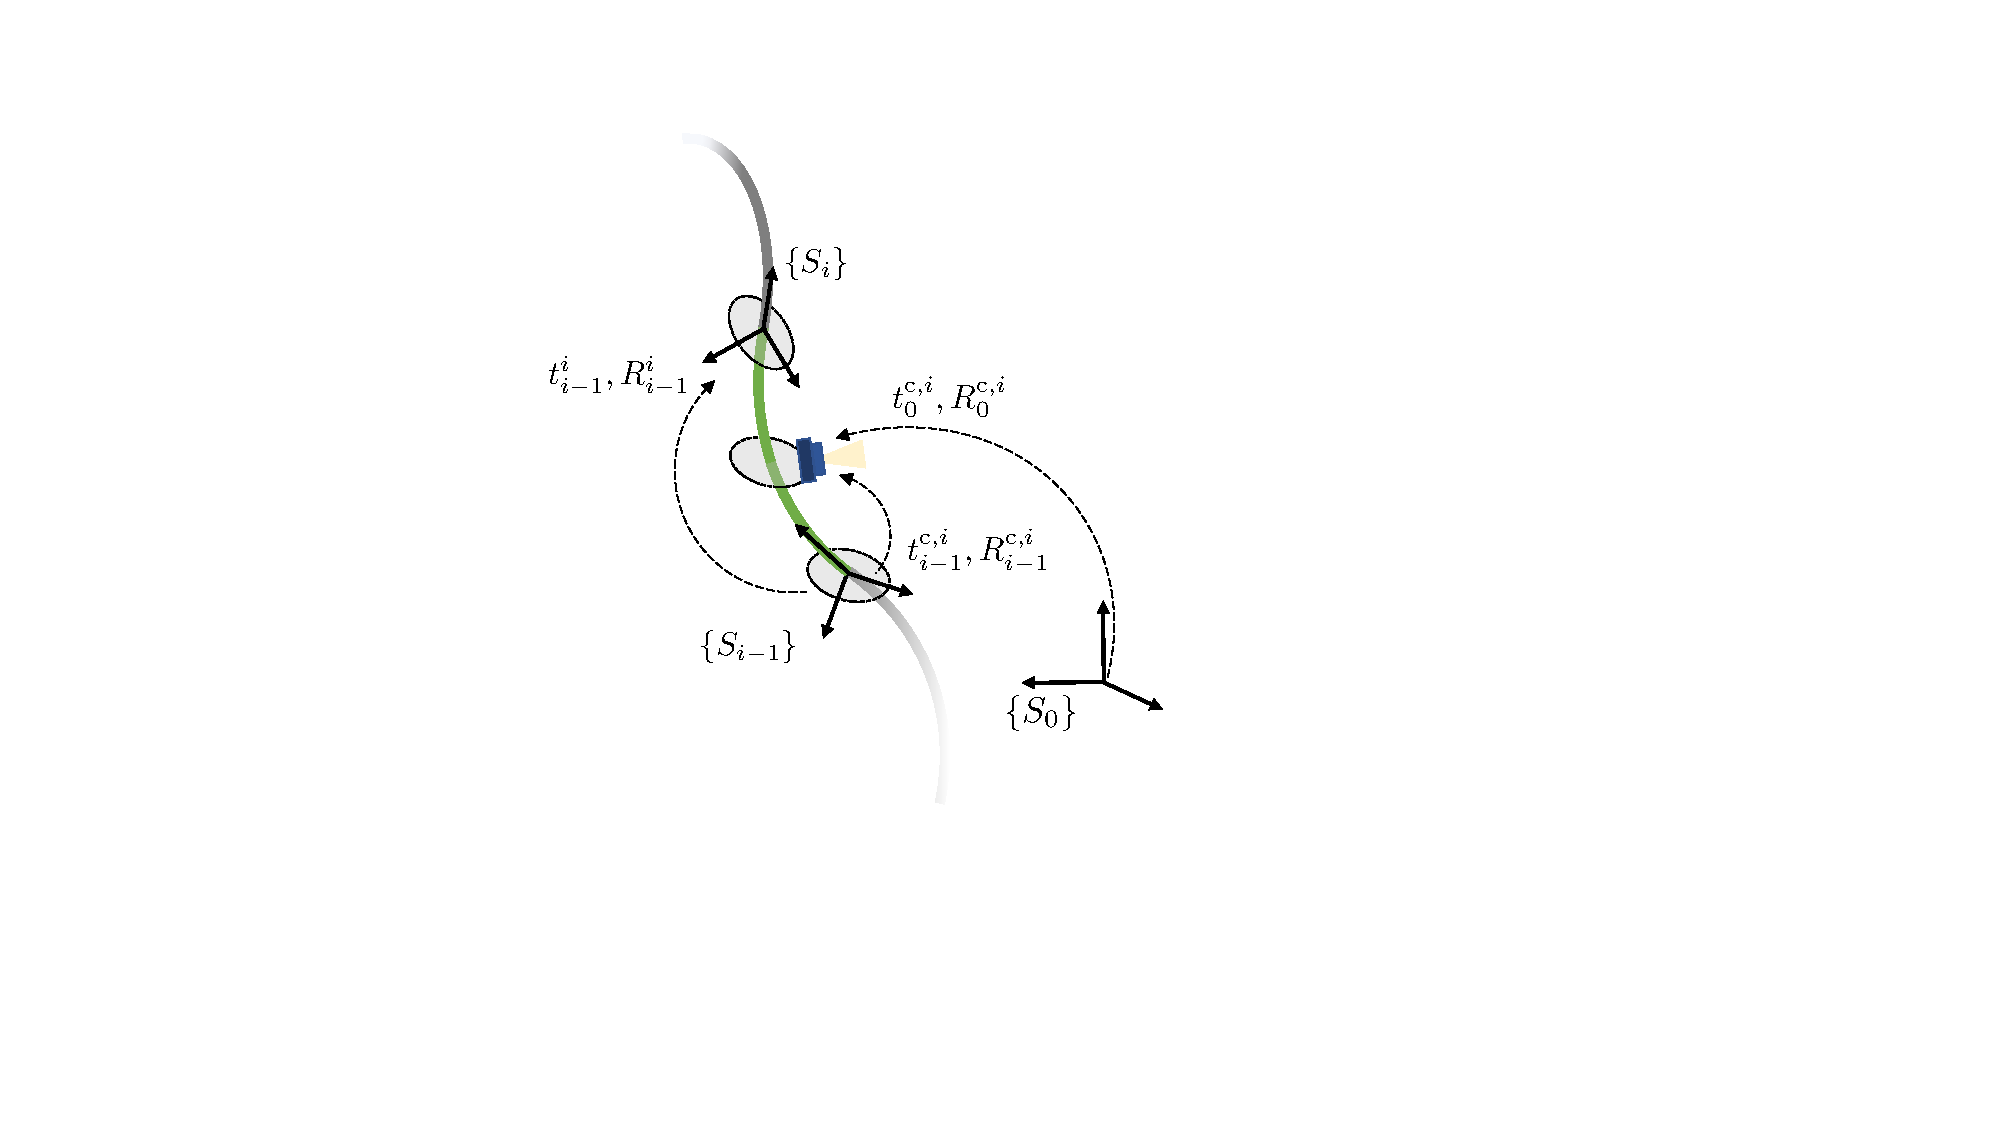
\includegraphics[width=0.24\columnwidth, trim = {0 0 0 0}, clip]{srslam/figures/kinematics_v2.pdf}\label{fig:srslam:kinematic_parameters} \label{fig:srslam:kinematics}}
     \caption{ Panel (a) shows a pictorial representation of the proposed perception strategy. Cameras are attached to a soft continuum robot. We propose to use ORB-SLAM~\cite{mur2017orb} to gather a pose estimate for each camera. The results are iteratively combined to extract local transformation, and refined by projecting the resulting postures onto the manifold of configurations attainable with the \gls{PCC} kinematics. The result is an estimation of the full shape within the selected kinematic description $\hat{q}$. Panel (b) reports the main quantities of the kinematic model of one segment. }
\end{figure*}
\section{Proposed architecture: Shape estimation with kinematics-aware SLAM}
\label{sec:srslam:pose_estimation}

In this work we propose to use \gls{SLAM} for proprioception of continuum soft robots. Common kinematic parametrizations for soft robots such as \gls{PCC}~\cite{webster2010design} or \gls{PCS}~\cite{renda2018discrete} model the soft arm to consist of multiple segments with independent kinematic state variables. 
In the following, we assume that the robot's model consists of $n_{\mathrm{S}}$ segments, and that a monocular camera is attached to each segment. We rely on a \gls{PCC} kinematic formulation. However, the proposed results can be directly generalized to the PCS case.
%
%We expect that there exists a constant coordinate transformation between the camera and one point along the center-line of the soft segment.
%
Our goal is to reconstruct the full shape (i.e., a configuration $q_i$ for each segment) of the soft robot from the stream of images recorded by the cameras.

Fig. \ref{fig:srslam:method_overview} shows an overview of the proposed architecture.
%
%Monocular \gls{SLAM} algorithms are able to estimate the pose of each camera as the robot arm follows a trajectory.
We use \gls{SLAM} algorithms such as monocular ORB-SLAM~\cite{mur2017orb} to estimate the pose of cameras attached to the soft robotic arm.  The pose estimation consists of 3D translation and rotations describing the relative camera movement from initial calibration to the current state ($\hat{t}_0^{\mathrm{c}_i},\hat{R}_0^{\mathrm{c}_i}$ in the figure). Then, the kinematic model is simultaneously used to refine the outputs of the SLAM and transform it to the desired estimation of the configurations ($\hat{q}_1,\hat{q}_3,\hat{q}_3$ in the figure). Starting from the base segment, and progressively iterating up until reaching the tip of the robot, we express translation and rotations in local coordinates, and we optimize the estimated configurations segment-by-segment starting at the proximal end by projecting the pose estimate into the 3D \gls{PCC} kinematics.
% This approach leverages known characteristics of the continuum soft robot and reduces the pose estimation error.

In the following subsections, we provide more details on the various components of this architecture.

\subsection{Background: Monocular ORB-SLAM}
We choose monocular ORB-SLAM~\cite{mur2017orb} for pose estimation of the camera locations. Although this technological solution has never been applied to soft robots, the algorithm itself is well established and its applications to mobile robotics widespread. As such, we  briefly describe here only the major steps of the algorithm.%, based on the pipeline in \ref{fig:srslam:algorithmpipeline}. 
 \begin{enumerate}
     \item \textbf{Map Initialization}: ORB-SLAM initializes a map of 3D points based on two video frames. The 3D points and relative camera pose are computed using triangulation of 2D ORB feature correspondences.
     \item \textbf{Tracking}: Once the map is initialized, the camera pose is estimated for each new frame by matching features in the current frame to features in the last key frame. The estimated camera pose is refined by tracking the local map.
     \item \textbf{Local Mapping}: If the current frame is identified as a key frame, it is used to create new 3D map points. At this stage, \gls{BA} is used to minimize re-projection errors by adjusting the camera pose and 3D points.
     \item \textbf{Loop Closure}: Loops are detected for each key frame by comparing it against all previous ones. % key frames using the bag-of-features approach~\cite{o2011introduction}. 
     %Any time a loop closure is detected, the pose graph is optimized to refine the camera poses of all the key frames.
     This information is used to optimize the poses.
 \end{enumerate}
An important aspect of \gls{SLAM} algorithms are key frames, which are a subset of video frames that contain cues for localization and tracking. Two consecutive key frames usually involve sufficient visual change. % In the end the algorithm returns the camera poses for each key frame.

\subsection{Projection into PCC-Kinematics}
Once the \gls{SLAM} algorithm provides us with the estimated camera poses, we want to interpret and correct them such as that they are coherent with the \gls{PCC} kinematic model.
%
In this paper, we consider the \emph{Delta} parametrization~\cite{della2020improved} of the \gls{PCC} kinematics, but the formulation could also be easily adapted to other kinematic parametrizations such as \gls{PCS}~\cite{renda2018discrete}.

% \begin{figure}[ht]
%     \centering
%     \includegraphics[width=1\columnwidth]{srslam/figures/kinematic_parameters.pdf}\label{fig:srslam:kinematic_parameters}
%     \\
%     \caption{One graphic showing the kinematic parameters for a multi-segment setup with multiple cameras and all used coordinate transformations.}
% \end{figure}

We show a pictorial representation of this kinematic model in Fig. \ref{fig:srslam:kinematics}. Each segment of original length $L_{0,i}$ is described with three configuration variables 
%
%\begin{equation}
    $q_i \in \mathbb{R}^{3} = \begin{pmatrix}\Delta_{x,i} & \Delta_{y,i} & \delta L_i\end{pmatrix}^\mathrm{T}$,
%\end{equation}
where $\delta L_i$ is segment's extension, and $\Delta_{x,i}$ and $\Delta_{y,i}$ are the differences of the arc lengths of the segment at a radial distance of $d_i$ from the center-line along both cardinal directions of the base~\cite{della2020improved}. The complete robot's configuration is $q \in \mathbb{R}^{3 n_{\mathrm{S}}}$. The coordinate transformation for segment $i$ from the base frame $\{ S_{i-1} \}$ into the tip frame $\{ S_{i} \}$ as a function of the configuration $q_i$ is given by~\cite{della2020improved}
\begin{equation}
\label{eq:srslam:transformation_improved_pcc}
\begin{split}
    R_{i-1}^{i} &= 
    \begin{pmatrix}
        1 + \frac{\Delta_{x,i}^2}{\Delta_{i}^2} \left ( \mathrm{c}_i - 1 \right ) & \frac{\Delta_{x,i} \Delta_{y,i}}{\Delta_{i}^2} \left ( \mathrm{c}_i - 1 \right ) & \frac{\Delta_{x,i}}{\Delta_i} \mathrm{s}_i\\
        \frac{\Delta_{x,i} \Delta_{y,i}}{\Delta_{i}^2} \left ( \mathrm{c}_i - 1 \right ) & 1 + \frac{\Delta_{y,i}^2}{\Delta_{i}^2} \left ( \mathrm{c}_i - 1 \right ) & \frac{\Delta_{y,i}}{\Delta_i} \mathrm{s}_i\\
        \frac{-\Delta_{x,i}}{\Delta_i} \mathrm{s}_i & \frac{-\Delta_{y,i}}{\Delta_i} \mathrm{s}_i & \mathrm{c}_i
    \end{pmatrix},\\
    \vspace{0.25em}
    t_{i-1}^{i} &= \frac{d_i ( L_{0,i}+\delta L_i)}{\Delta_i^2}
    \begin{pmatrix}
        \Delta_{x,i} (1 - \mathrm{c}_i) & \Delta_{y,i} (1 - \mathrm{c}_i) & \Delta_{i} \mathrm{s}_i
    \end{pmatrix}^{\mathrm{T}},
\end{split}
\end{equation}
where we substituted $\Delta_i = \sqrt{\Delta_{x,i}^2 + \Delta_{y,i}^2}$, $\mathrm{s}_i = \sin \left ( \frac{\Delta_i}{d_i} \right )$, and $\mathrm{c}_i = \cos \left ( \frac{\Delta_i}{d_i} \right )$ for conciseness.

We describe the coordinate frame of camera $i$ with $\{ S_{\mathrm{c}_i} \}$. It is assumed that there exists a fixed transformation $T_{\check{\mathrm{c}},i}^{\mathrm{c}_i} \in \mathbb{R}^{4 \times 4}$ from frame $\{ S_{\check{\mathrm{c}},i} \}$ to the camera frame $\{ S_{\mathrm{c}_i} \}$. 
$\{ S_{\check{\mathrm{c}},i} \}$ is localized at a distance $l_{\mathrm{c}_i}$ along the center-line from the base of segment $i$. 
The transformation $T_{i-1}^{\check{\mathrm{c}},i}(q_{\check{c},i})$ from the base to the frame $\{ S_{\check{\mathrm{c}},i} \}$ can be found with \eqref{eq:srslam:transformation_improved_pcc} by plugging in the adjusted configuration $q_{\check{c},i}$ defined as
\begin{equation}\label{eq:srslam:camera_configuration}
    q_{\check{c},i} = \frac{l_{\mathrm{c}_i}}{L_{0,i}} q_i,
\end{equation}
and the adjusted original length  $l_{\mathrm{c}_i}$.

The \gls{SLAM} algorithm provides a pose estimate for the translation $\hat{t}_{\mathrm{c},\mathrm{t}0,i}^{\mathrm{c}_i} \in \mathbb{R}^3$ and rotation $\hat{R}_{\mathrm{c},\mathrm{t}0,i}^{\mathrm{c}_i} \in \mathbb{R}^{3 \times 3}$ relative to the known initial reference frame of the camera $\{ S_{\mathrm{c},\mathrm{t}0,i} \}$. 
Thus, we first transform the pose estimates to the inertial frame of the robot $\{ S_0 \}$
\begin{equation}
    \begin{pmatrix}
        \hat{t}_{0}^{\mathrm{c}_i}\\
        1
    \end{pmatrix}
    = T_0^{\mathrm{c},\mathrm{t}0,i}
    \begin{pmatrix}
        \hat{t}_{\mathrm{c},\mathrm{t}0,i}^{\mathrm{c}_i}\\
        1
    \end{pmatrix},
    \quad
    \hat{R}_{0}^{\mathrm{c}_i} = R_0^{\mathrm{c},\mathrm{t}0,i} \hat{R}_{\mathrm{c},\mathrm{t}0,i}^{\mathrm{c}_i}.
\end{equation}

We introduce the following notations for the \gls{PCC} kinematics
\begin{equation}\label{eq:srslam:Pi}
\begin{split}
    \hat{t}_{i-1}^{\mathrm{c}_i} &= \Pi_\mathrm{t}(\hat{q}_i) = 
    \hat{T}_{i-1}^{\check{\mathrm{c}},i} \left (\frac{l_{\mathrm{c}_i}}{L_{0,i}} \hat{q}_i \right )
    t_{\check{\mathrm{c}},i}^{\mathrm{c}_i}\\
    \hat{R}_{i-1}^{\mathrm{c}_i} &= \Pi_\mathrm{R}(\hat{q}_i) =
    \hat{R}_{i-1}^{\check{\mathrm{c}},i} \left (\frac{l_{\mathrm{c}_i}}{L_{0,i}} \hat{q}_i \right )
    R_{\check{\mathrm{c}},i}^{\mathrm{c}_i},
\end{split}
\end{equation}
where $\hat{t}_{i-1}^{\check{\mathrm{c}},i}$ and $\hat{R}_{i-1}^{\check{\mathrm{c}},i}$ describe the translation and rotation from the base of the segment to the camera frame according to the \gls{PCC} kinematic model for an estimated configuration of the the segment $\hat{q}_i$. $\hat{T}_{i-1}^{\check{\mathrm{c}},i}(q_{\check{c},i})$ and $\hat{R}_{i-1}^{\check{\mathrm{c}},i}(q_{\check{c},i})$ are based on \eqref{eq:srslam:transformation_improved_pcc} and a function of the adjusted configuration $q_{\check{c},i}$ referenced in \eqref{eq:srslam:camera_configuration}.

Additionally, the pose estimates by the \gls{SLAM} algorithm need to be transformed to the base frame of segment $i$. Thus, we introduce the following
\begin{equation}\label{eq:srslam:Psi}
\begin{split}
    \hat{t}_{i-1}^{\mathrm{c}_i} &= \Psi_\mathrm{t}(q_1 \dots q_{i-1}, \hat{t}_{0}^{\mathrm{c}_i}) =
    \prod_{\tilde{i}=1}^{i-1} \left ( T_{\tilde{i}-1}^{\tilde{i}} \left (\hat{q}_{\tilde{i}} \right )  \right )^\mathrm{T}
    \begin{pmatrix}
        \hat{t}_{0}^{\mathrm{c}_i}\\
        1
    \end{pmatrix},\\
    \hat{R}_{i-1}^{\mathrm{c}_i} &= \Psi_\mathrm{R}(q_1 \dots q_{i-1}, \hat{R}_{0}^{\mathrm{c}_i}) =
    \prod_{\tilde{i}=1}^{i-1} \left ( R_{\tilde{i}-1}^{\tilde{i}} \left (\hat{q}_{\tilde{i}} \right )  \right )^\mathrm{T}
    \hat{R}_{0}^{\mathrm{c}_i}.
\end{split}    
\end{equation}

Next, we define a cost function to optimize the pose estimate by projecting them into the \gls{PCC}-kinematics
% Please note, that we do not include the orientation estimate $\hat{R}_{0}^{\mathrm{c}_i}$ by the \gls{SLAM} algorithm in the cost function.
%
\begin{equation}\label{eq:srslam:cost_fun}
    \min_{\hat{q}} \sum_{i=1}^{n_\mathrm{S}} f_{\mathrm{t},i}(\hat{q}) + \lambda_\mathrm{R} f_{\mathrm{R},i}(\hat{q}),
\end{equation}
with
\begin{equation}\label{eq:srslam:cost_fun_ingredients}
\begin{split}
    f_{\mathrm{t},i}(\hat{q}) &=
    \big\lVert 
    \Pi_\mathrm{t}(\hat{q}_i) - \Psi_\mathrm{t}(q_1 \dots q_{i-1}, \hat{t}_{0}^{\mathrm{c}_i})
    \big\rVert_2,\\
    f_{\mathrm{R},i}(\hat{q}) &=
    \big\lVert 
    \Pi_\mathrm{R}(\hat{q}_i) - \Psi_\mathrm{R}(q_1 \dots q_{i-1}, \hat{R}_{0}^{\mathrm{c}_i})
    \big\rVert_F,
\end{split}
\end{equation}
where the Euclidean norm is used to compute the translational error between the predicted translation by the \gls{PCC} kinematic model and the estimated translation by \gls{SLAM}. The rotational error is weighted with $\lambda_\mathrm{R}$ and computed with the Frobenius norm between the predicted rotation matrix by the \gls{PCC} kinematics and the estimated orientation by \gls{SLAM} represented as a rotation matrix as well.

Please note, that the optimization of the configuration estimate $\hat{q}$ can be decoupled for each segment. 
We start by optimizing the configuration of the first segment $\hat{q}_1$ based on $\Psi_\mathrm{t}(\hat{t}_{0}^{\mathrm{c},1})$ and $\Psi_\mathrm{R}(\hat{R}_{0}^{\mathrm{c},1})$. Next, we optimize the configuration of the second segment $\hat{q}_2$ taking into account the already optimized configuration of segment one in $\Psi_\mathrm{t}(\hat{q}_1, \hat{t}_{0}^{\mathrm{c},2})$ and $\Psi_\mathrm{R}(\hat{q}_1, \hat{R}_{0}^{\mathrm{c},2})$. 
Subsequently, we move on to optimize the remaining segments sequentially as described by Algorithm~\ref{alg:srslampose_estimation}. This procedure is also graphically represented by the right side of Fig. \ref{fig:srslam:method_overview}.

\begin{algorithm}[hbt!]
\caption{Pose estimation for soft robots through SLAM}\label{alg:srslampose_estimation}
\begin{algorithmic}
\REQUIRE $o \in \mathbb{R}^{n_\mathrm{S}}$ \COMMENT{Observations of all cameras}
\ENSURE $\hat{q} \in \mathbb{R}^{3 n_\mathrm{S}}$ \COMMENT{Estimated robot configuration}
\STATE $i \gets 1$
\WHILE{$i \leq n_\mathrm{S}$}
    \vspace{0.25em}
    \STATE $\hat{t}_{0}^{\mathrm{c}_i} \gets T_0^{\mathrm{c},\mathrm{t}0,i} \: \mathrm{SLAM}_\mathrm{t}(o_i)$ \COMMENT{Translational est. SLAM}
    \vspace{0.25em}
    \STATE $\hat{R}_{0}^{\mathrm{c}_i} \gets R_0^{\mathrm{c},\mathrm{t}0,i} \: \mathrm{SLAM}_\mathrm{R}(o_i)$ \COMMENT{Rotational est. SLAM}
    \vspace{0.25em}
    \STATE $f_{\mathrm{t},i}(\hat{q}) \gets
    \big\lVert 
    \Pi_\mathrm{t}(\hat{q}_i) - \Psi_\mathrm{t}(q_1 \dots q_{i-1}, \hat{t}_{0}^{\mathrm{c}_i})
    \big\rVert_2$
    \vspace{0.25em}
    \STATE $f_{\mathrm{R},i}(\hat{q}) \gets
    \big\lVert 
    \Pi_\mathrm{R}(\hat{q}_i) - \Psi_\mathrm{R}(q_1 \dots q_{i-1}, \hat{R}_{0}^{\mathrm{c}_i})
    \big\rVert_F$
    \vspace{0.25em}
    \STATE $f_{c,i}(\hat{q}) \gets f_{\mathrm{t},i}(\hat{q}) + \lambda_\mathrm{R} f_{\mathrm{R},i}(\hat{q})$ \COMMENT{Cost function for $\hat{q}_i$}
    \vspace{0.25em}
    \STATE $\hat{q}_i \gets \argmin_{\hat{q_i}} f_c(\hat{q})$
    \vspace{0.25em}
    \STATE $i \gets i + 1$
\ENDWHILE
\end{algorithmic}
\end{algorithm}

\section{Simulations}
\label{sec:srslam:simulations}

We quantitatively evaluate our approach in simulation for one soft robotic segment with a camera attached to the tip of the robot. 
We first compute trajectories that behave according to \gls{PCC} kinematics. 
Next, we render photo-realistic images for the camera attached to the tip of the segment for every time step using a virtual environment implemented in Blender. Subsequently, we process the synthetic camera images with the ORB-SLAM~\cite{mur2017orb} algorithm and projected the estimated poses of the tip of the segment into the \gls{PCC} kinematic model as outlined in Section~\ref{sec:srslam:pose_estimation}. Finally, we compare the estimated poses against the ground truth and statistically evaluate the \gls{RMSE} both for translational and rotational estimates. More details follow.

\subsection{System}\label{sub:srslam:simulations_system}
We consider a soft robotic segment of diameter \SI{20}{mm} diameter and with varying lengths $L_{0,1}$ between \SI{15}{cm} and \SI{100}{cm}.
As the camera is attached to the tip of the segment, we set $l_{\mathrm{c}_1} = L_{0,1}$ and define $T_{\check{\mathrm{c}},1}^{\mathrm{c},1} = \mathbb{I}^4$.

\subsection{Trajectories and calibration sequence}\label{sub:srslam:trajectories}
Three different trajectories are considered for the simulated movement of the soft robotic segment and its attached virtual camera. While the first one represents a planar side bending, the second one describes an “8” shape with the tip, and the last one covers a lobe of the “8”. 
Those trajectories were commanded in $\Delta_{x,1}$ and $\Delta_{y,1}$, with the following mathematical formulas:
\begin{equation}\label{eq:srslam:trajectory_parametrization}
    \Delta_{x,1} = L_{0,1} A_x \sin(2 \pi f_x) \qquad \Delta_{y,1} = L_{0,1} A_y \sin(2 \pi f_y),
\end{equation}
with $L_{0,1}$ the unextended length of the robot, $A_x$ and $A_y$ amplitudes of the sinusoids and $f_x$ and $f_y$ frequencies of the sinusoids.
The parameters $f_x$ and $f_y$ are defined as follows with $k$ representing the current time index:
\begin{equation}
    f_x = \frac{F_x (k-1)}{n_{\mathrm{t}}}, \qquad f_y = \frac{F_y (k-1)}{n_{\mathrm{t}}}.
\end{equation}
Please note that these trajectories do not contain any segment elongation. 
We list the chosen amplitudes and frequencies of the trajectories in Table~\ref{tab:srslam:trajectory_params}. Each trajectory is generated considering different robot lengths, namely \SI{15}{cm}, \SI{30}{cm} and \SI{100}{cm}. The number of time steps $n_{\mathrm{t}}$ is chosen at $120$. 
The commanding of $\Delta_{x,1}$ and $\Delta_{y,1}$ is such that the amplitude and frequency of the trajectory are independent of the number of frames (i.e., time steps).
In Figure~\ref{fig:srslam:trajectories}, we show a 3D visualization of the trajectories corresponding to a segment length of \SI{15}{cm}.

\begin{table}
\centering
\caption{Parameters of the implemented trajectories. We list the amplitudes and the frequencies of the trajectories parametrized by $\Delta_{x,1}$ and $\Delta_{y,1}$ as specified in \eqref{eq:srslam:trajectory_parametrization}.}
% \begin{scriptsize}
\begin{tabular}{lcccc}\toprule
\textbf{Trajectory} & $A_x$ & $A_y$ & $F_x$ & $F_y$\\
\midrule
Trajectory 1: planar side bending & 0.1 & 0 & 0.5 & 0\\
Trajectory 2: half 8-shape & 0.05 & 0.05 & 1 & 0.5\\
Trajectory 3: full 8-shape & 0.05 & 0.05 & 2 & 1\\
\bottomrule
\end{tabular}
% \end{scriptsize}
\label{tab:srslam:trajectory_params}
\end{table}

\begin{figure*}[ht]
  \centering
  \subfigure[Trajectory 1]{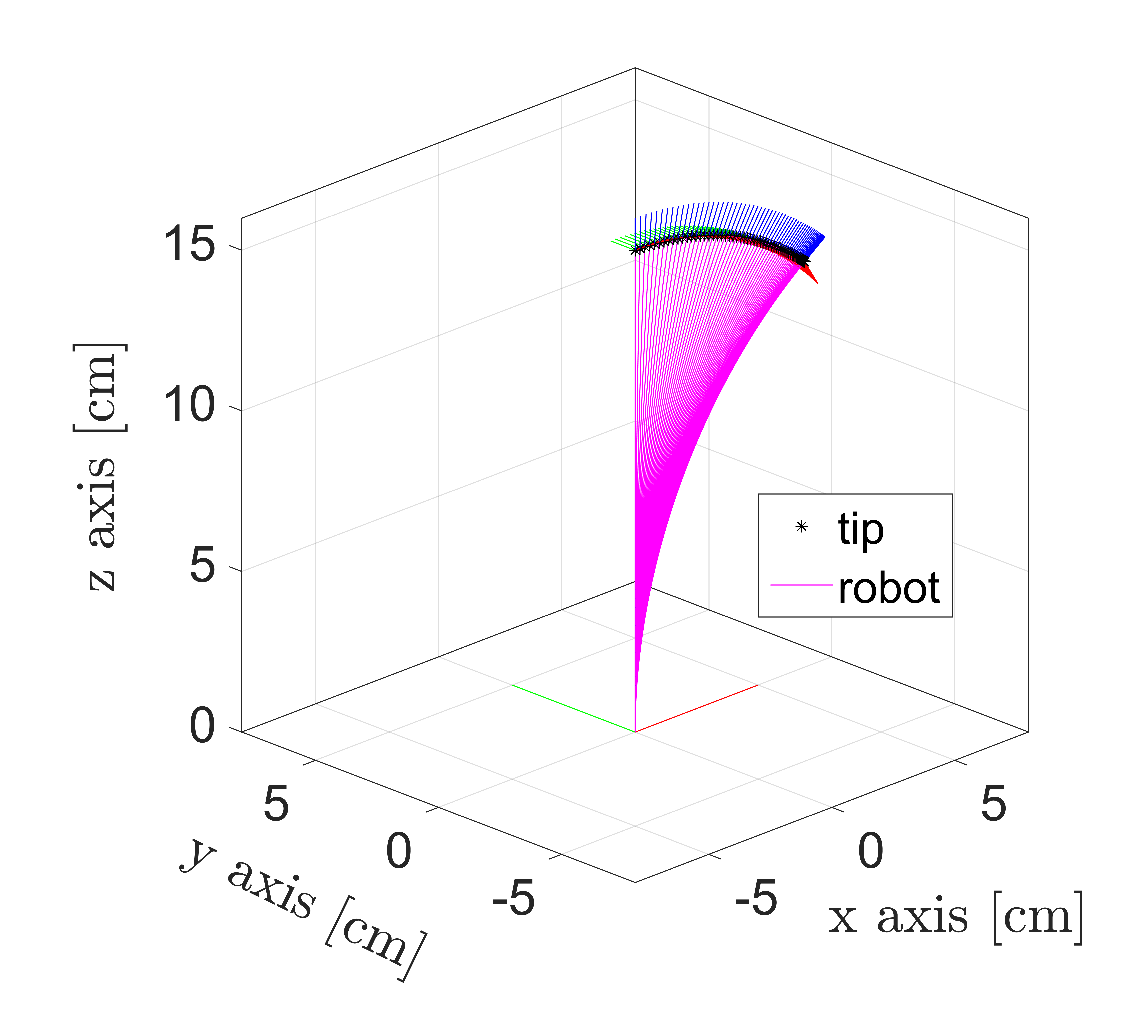
\includegraphics[width=0.21\textwidth]{srslam/figures/t1_l15_v3.0.eps}\label{fig:srslam:traj1}}
  \hspace{0.005\textwidth}% \hfill% or \hspace{5mm} or \hspace{0.3\textwidth}
  \subfigure[Trajectory 2]{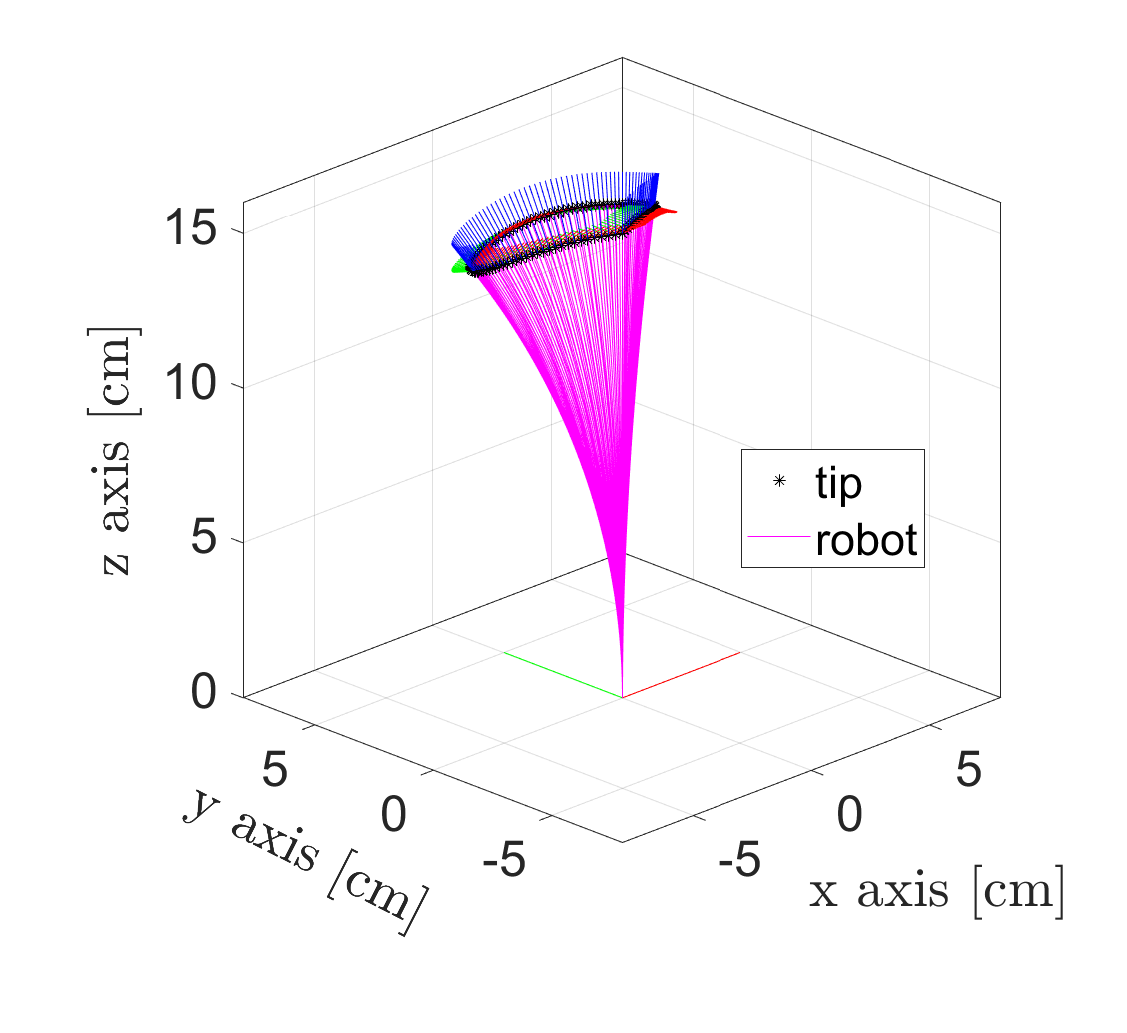
\includegraphics[width=0.21\textwidth]{srslam/figures/t2_l15_v3.2.eps}\label{fig:srslam:traj2}}\hspace{0.005\textwidth}% \hfill% or \hspace{5mm} or \hspace{0.3\textwidth}
  \subfigure[Trajectory 3]{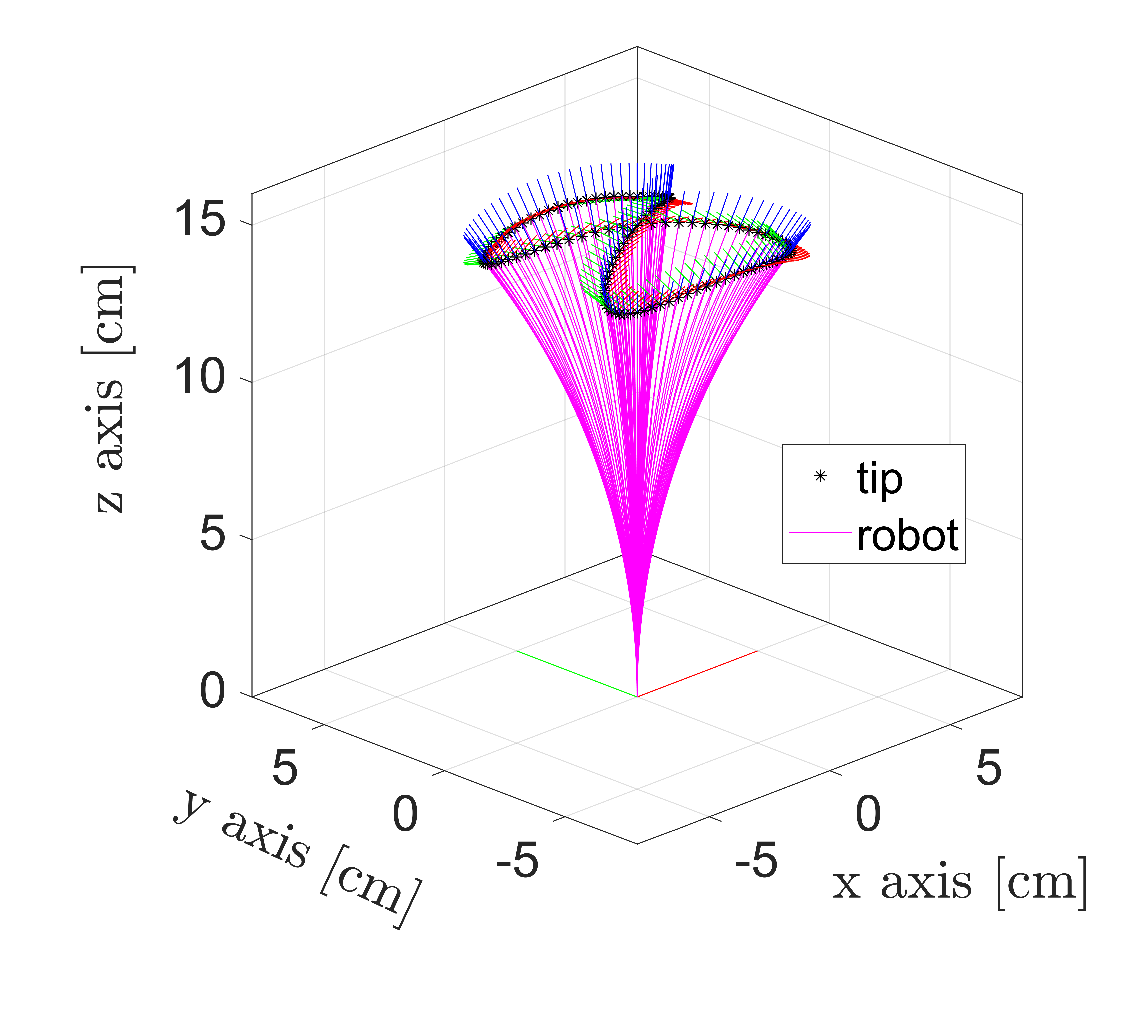
\includegraphics[width=0.21\textwidth]{srslam/figures/t3_l15_v3.1.eps}\label{fig:srslam:traj3}}\hfill
  \subfigure[Virtual interior scene]{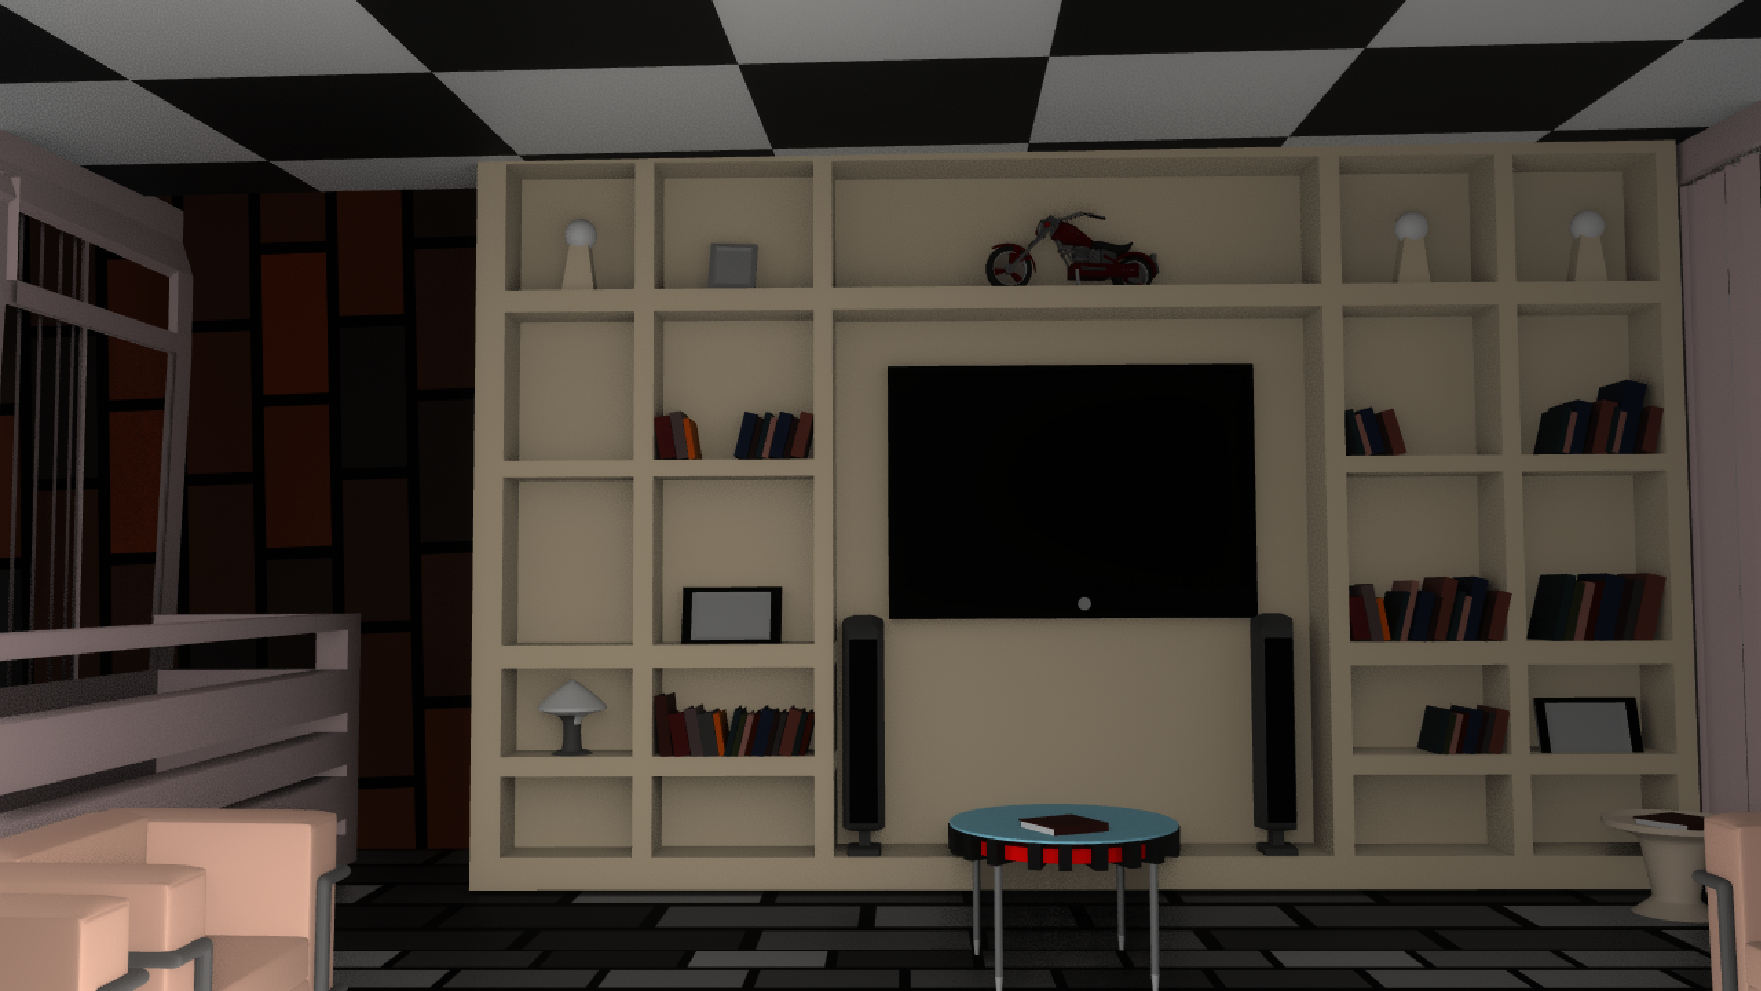
\includegraphics[width=0.3\textwidth]{srslam/figures/interior_scene.pdf}\label{fig:srslam:interior_scene}}
  \caption{3D visualization of the three trajectories used in our simulations and experiments for a segment with \SI{15}{cm} length. In magenta, we visualize the trajectory of the full robot, and in black, the tip positions. Additionally, the tip orientation (red = x-axis, green = y-axis, blue = z-axis) is displayed. The virtual interior scene used for the Blender renderings is presented in the last column.}
  \label{fig:srslam:trajectories}
\end{figure*}

In addition to the robot trajectory, a calibration sequence trajectory is designed to initialize the \gls{SLAM} map. 
It is good practice to move the camera parallel to the scene captured. Accordingly, we decide to move the camera into the $x$ cardinal direction of the segment base frame with the translation distance proportional to the robot length.

\subsection{Rendering of synthetic images}
The rendering software Blender allows us, among other things, to load a 3D model of the environment, follow customized trajectories with a virtual camera, and render photo-realistic synthetic pictures of the environment from the chosen camera perspective. We use an interior scene published by \href{https://www.nextwavemultimedia.com/html/3dblendermodel.html}{Nextwave Multimedia}. We report a view of the scene in Fig. \ref{fig:srslam:interior_scene}.
The virtual camera is set to be perspective with a focal length of \SI{30}{mm}.
For each run, we randomly initialize the trajectory at one of seven predefined launch points in the indoor environment to diversify the coverage of the environment.
The x-, y-, and z-coordinates of the seven initial positions have a standard deviation of \SI{0.5}{m}, \SI{0.2}{m}, \SI{0.4}{m} respectively. The initial orientation represented in XYZ Euler angles varies with a standard deviation of \SI{0.05}{rad}, \SI{0.13}{rad}, and \SI{1.17}{rad}.
For each trajectory, we render $120$ synthetic images along the trajectory and save them to a folder for later offline processing by the ORB-SLAM~\cite{mur2017orb} algorithm. Fig. \ref{fig:srslam:sequences_of_stills_simulations_cropped} reports a few representative stills of what the robot sees during one execution of the three trajectories discussed above.

\begin{figure*}
    \centering
    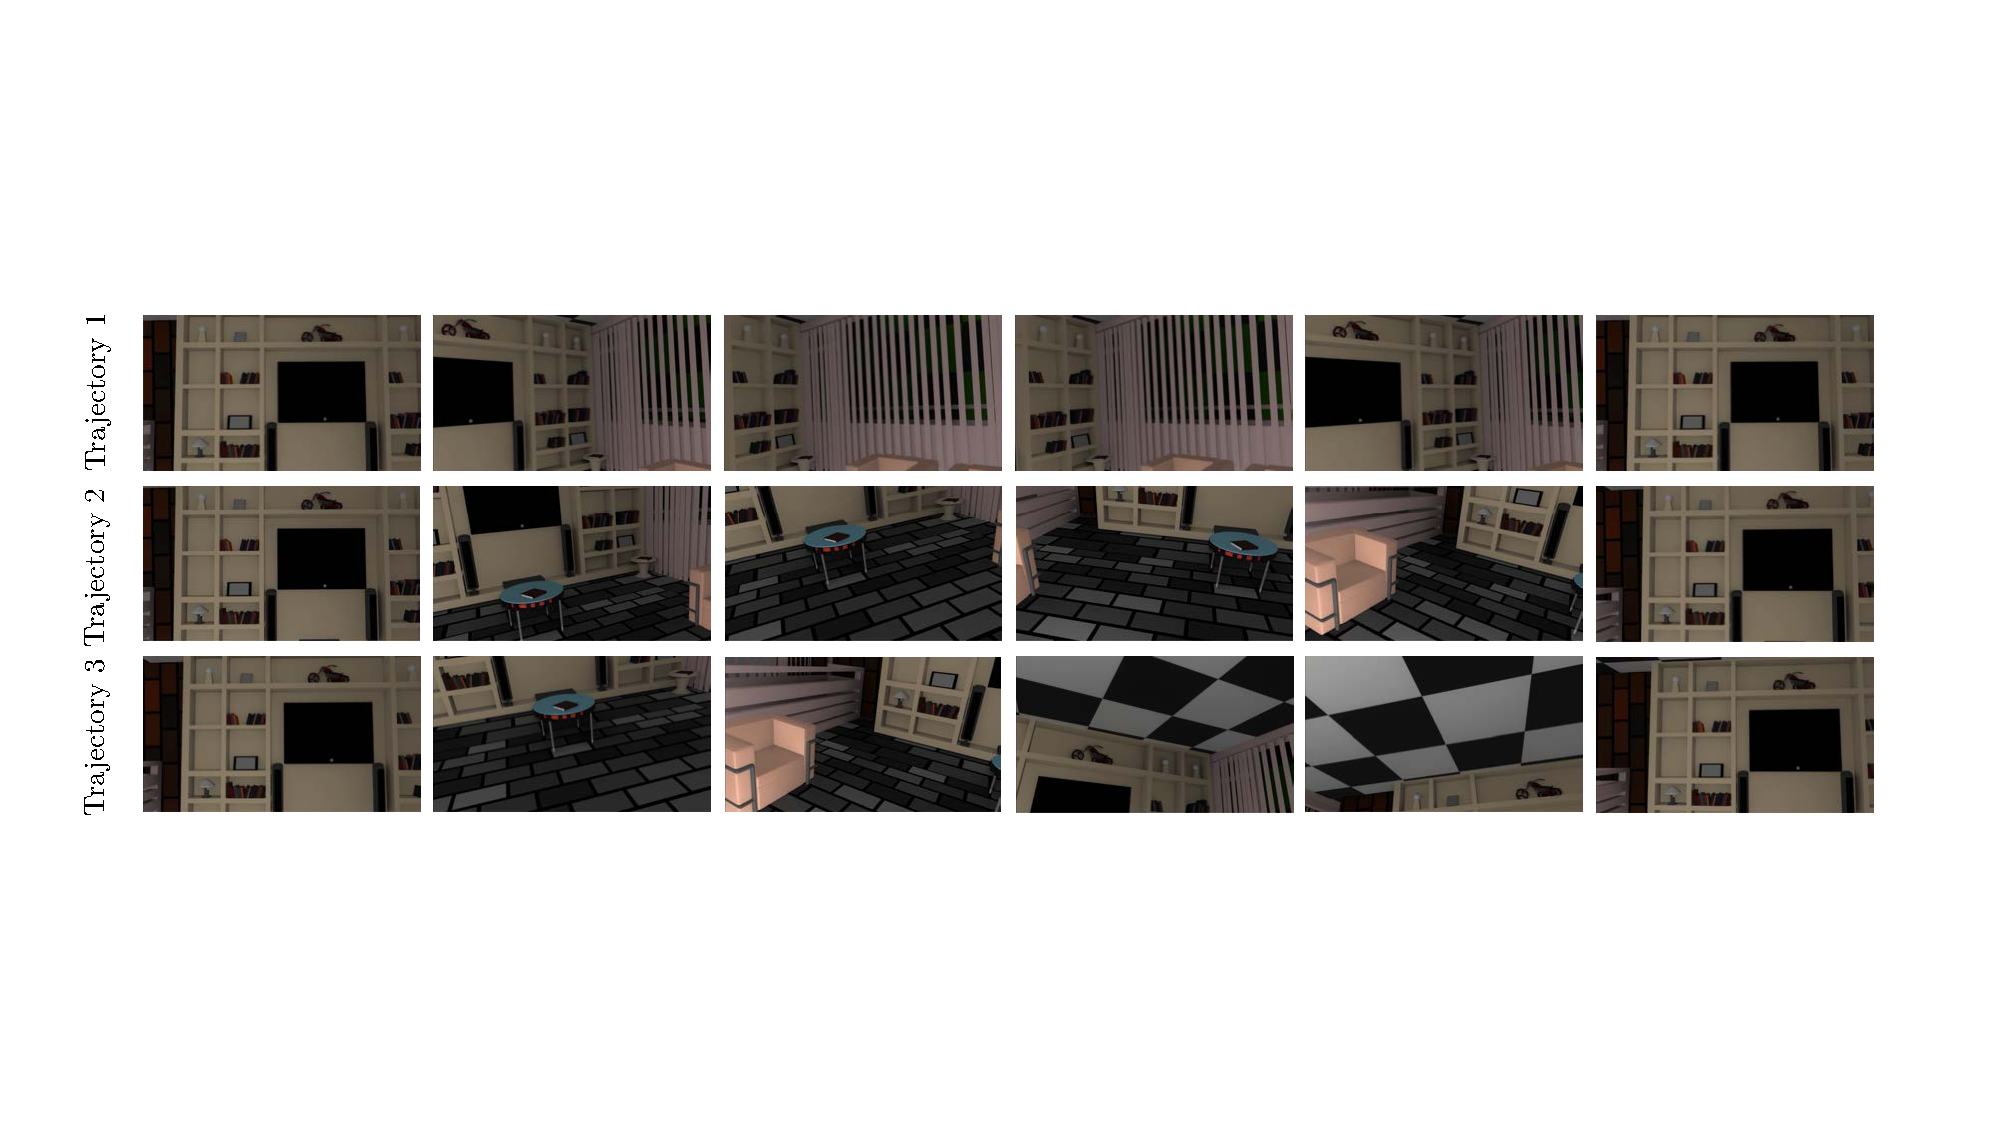
\includegraphics[width=0.9\textwidth]{srslam/figures/graphic_sequences_of_stills_simulations_compressed.pdf}
    \caption{Sequence of stills showing the rendered images by the virtual camera in Blender for three different trajectories and a robot segment of length \SI{15}{cm}. The trajectories are visualized in Figure~\ref{fig:srslam:trajectories}.}
    \label{fig:srslam:sequences_of_stills_simulations_cropped}
\end{figure*}

\subsection{Implementation of ORB-SLAM}
The synthetic images along the trajectory are processed offline by the ORB-SLAM~\cite{mur2017orb} algorithm. We rely on the official MATLAB implementation of ORB-SLAM. While we run our simulations offline to decouple any delays by the rendering and/or \gls{SLAM} pipeline, we would like to point out that other ORB-SLAM implementations, such as, for example, in C++, are able to be run in real-time at frame rates of between \SI{10}{Hz} to \SI{30}{Hz}~\cite{mur2017orb}.

\subsection{Projection into PCC kinematics}
The trade-off parameter $\lambda_\mathrm{R}$ between the rotational and the translational error in the cost function \eqref{eq:srslam:cost_fun} was manually tuned and set to $\lambda_\mathrm{R}=0.4$.
As the simulations do not contain any elongations of the segment, we set $\delta L_1 = 0$ in \eqref{eq:srslam:transformation_improved_pcc}. 
We solve the optimization problem outlined in \eqref{eq:srslam:cost_fun} using nonlinear least-squares with the Levenberg-Marquardt solver~\cite{levenberg1944method, marquardt1963algorithm} implemented in MATLAB as \emph{lsqnonlin}.

\subsection{Evaluation metrics}
To quantitatively evaluate the performance of our proposed approach, we introduce error metrics for both the translation and orientation estimates.
%
We measure the translational pose prediction error with a relative \gls{RMSE} $e_\mathrm{t}$
\begin{equation}\label{eq:srslam:evaluation_translational_error}
    e_\mathrm{t} = \frac{\sqrt{\sum_{t=1}^{n_\mathrm{t}} \left (\lVert \hat{t}_{0,t}^{\mathrm{c},1} - t_{0,t}^{\mathrm{c},1} \rVert_2 \right )^2}}{\sqrt{n_\mathrm{t}} \; l_\mathrm{traj}},
\end{equation}
where $l_\mathrm{traj}$ corresponds to the length of the trajectory and $n_\mathrm{t}$ the total number of data points along the trajectory. Similarly, we leverage the Frobenius norm for the rotational error $e_\mathrm{R}$
\begin{equation}\label{eq:srslam:evaluation_rotational_error}
    e_\mathrm{R} = \sqrt{\sum_{t=1}^{n_\mathrm{t}} \frac{\left (\big\lVert \hat{R}_{0,t}^{\mathrm{c},1} - R_{0,t}^{\mathrm{c},1} \big\rVert_F \right )^2}{n_\mathrm{t}}}.
\end{equation}
As torsion can often be neglected for soft robotic arms, we state the angle error for the orientation of the local z-axis of the tip of the segment for intuitive analysis of the orientation estimates. First, the unit vector of the local z-axis $\{ o_{1} \}_{0}$ is computed in the base frame $\{ S_0 \}$
\begin{equation}
    \{ o_1 \}_0 = R_{0,t}^{1}\begin{pmatrix}0 & 0 & 1\end{pmatrix}^\mathrm{T},
    \quad
    \{ \hat{o}_1 \}_0 = \hat{R}_{0,t}^{1}\begin{pmatrix}0 & 0 & 1\end{pmatrix}^\mathrm{T},
\end{equation}
which allows us to subsequently compute the angle error between the ground-truth z-axis of the tip $\{ o_1 \}_0$ and the estimated z-axis $ \{ \hat{o}_1 \}_0$
\begin{equation}\label{eq:srslam:evaluation_angle_error}
    e_{\theta_z} = \sqrt{\sum_{t=1}^{n_\mathrm{t}} \frac{\left (\arccos \left ( \{ o_1 \}_0 \cdot \{ \hat{o}_1 \}_0 \right ) \right )^2}{n_\mathrm{t}}}.
\end{equation}

\subsection{Results}\label{sub:srslam:simulation_results}
% \begingroup
% \setlength{\tabcolsep}{2.0pt} % Default value: 6pt
% \renewcommand{\arraystretch}{1} % Default value: 1
\begin{table*}
\centering
\caption{Relative \gls{RMSE} [\%] for translations as referenced in \eqref{eq:srslam:evaluation_translational_error} of various trajectories and of robot segments with different lengths (\SI{15}{cm}, \SI{30}{cm}, \SI{100}{cm}). We state the error as $\text{mean} \pm \text{stdev} \; (\min, \max)$ and compute the statistics over seven trials from different initial poses.}
\begin{tabular}{cclll}\toprule
\textbf{Trajectory} & \textbf{Optimization} & $L_{0,1} = \SI{15}{cm}$ & $L_{0,1} = \SI{30}{cm}$ & $L_{0,1} = \SI{100}{cm}$\\
\midrule
Trajectory 1 & No & $9 \pm 3 \; (5, 12)$ & $7 \pm 3 \; (3, 13)$ & $3 \pm 2 \; (1, 7)$ \\
Trajectory 1 & Yes & $0.4 \pm 0.2 \; (0.3, 0.8)$ & $2 \pm 1 \; (0, 4)$ & $1.0 \pm 0.7 \; (0.5, 2.3)$ \\
\midrule
Trajectory 2 & No & $9 \pm 4 \; (4, 17)$ & $6 \pm 2 \; (3, 8)$ & $1.9 \pm 0.9 \; (1.0, 3.0)$ \\
Trajectory 2 & Yes & $0.7 \pm 0.7 \; (0.3, 1.8)$ & $0.7 \pm 0.4 \; (0.2, 1.2)$ & $0.6 \pm 0.3 \; (0.3, 0.9)$ \\
\midrule
Trajectory 3 & No & $6 \pm 5 \; (3, 16)$ & $2.6 \pm 0.6 \; (1.7, 3.3)$ & $6 \pm 14 \; (1, 37)$ \\
Trajectory 3 & Yes & $2 \pm 3 \; (0, 9)$ & $0.5 \pm 0.3 \; (0.1, 0.8)$ & $2 \pm 5 \; (0, 15)$ \\
\bottomrule
\end{tabular}
\label{tab:srslam:results_simulations_translation}
\end{table*}
% \endgroup

\iffalse
\begin{table*}
\centering
\caption{Absolute \gls{RMSE} [-] for rotations computed with the Frobenius norm between rotation matrices of various trajectories and of robots with various lengths as referenced in \eqref{eq:srslam:evaluation_rotational_error}. We state the error as $\text{mean} \pm \text{stdev} \; (\min, \max)$ and compute the statistics over seven trials from different initial poses.}
\begin{tabular}{cclll}\toprule
\textbf{Trajectory} & \textbf{Optimization} & $L_{0,1} = \SI{15}{cm}$ & $L_{0,1} = \SI{30}{cm}$ & $L_{0,1} = \SI{100}{cm}$\\
\midrule
    Trajectory 1 & No & $0.010 \pm 0.004 \; (0.003, 0.015)$ & $0.016 \pm 0.007 \; (0.008, 0.027)$ & $0.027 \pm 0.017 \; (0.010, 0.051)$ \\
    Trajectory 1 & Yes & $0.007 \pm 0.002 \; (0.003, 0.010)$ & $0.012 \pm 0.007 \; (0.004, 0.023)$ & $0.027 \pm 0.019 \; (0.013, 0.062)$ \\
    \midrule
    Trajectory 2 & No & $0.02 \pm 0.02 \; (0.01, 0.05)$ & $0.011 \pm 0.006 \; (0.005, 0.022)$ & $0.015 \pm 0.008 \; (0.006, 0.025)$ \\
    Trajectory 2 & Yes & $0.02 \pm 0.02 \; (0.00, 0.06)$ & $0.016 \pm 0.009 \; (0.003, 0.025)$ & $0.019 \pm 0.008 \; (0.009, 0.030)$ \\
    \midrule
    Trajectory 3 & No & $0.1 \pm 0.2 \; (0.0, 0.4)$ & $0.010 \pm 0.002 \; (0.006, 0.012)$ & $0.2 \pm 0.4 \; (0.0, 1.1)$ \\
    Trajectory 3 & Yes & $0.1 \pm 0.2 \; (0.0, 0.4)$ & $0.02 \pm 0.01 \; (0.00, 0.034)$ & $0.2 \pm 0.3 \; (0.0, 0.9)$ \\
\bottomrule
\end{tabular}
\label{tab:srslam:results_simulations_rotation_frobenius}
\end{table*}

\begin{table*}
\centering
\caption{Absolute \gls{RMSE} [rad] for rotations computed with dot product \textcolor{red}{...}. We state the error as $\text{mean} \pm \text{stdev} \; (\min, \max)$ and compute the statistics over seven trials from different initial poses.}
\begin{tabular}{cclll}\toprule
\textbf{Trajectory} & \textbf{Optimization} & $L_{0,1} = \SI{15}{cm}$ & $L_{0,1} = \SI{30}{cm}$ & $L_{0,1} = \SI{100}{cm}$\\
\midrule
    Trajectory 1 & No & $0.005 \pm 0.002 \; (0.002, 0.007)$ & $0.009 \pm 0.005 \; (0.004, 0.018)$ & $0.02 \pm 0.01 \; (0.01, 0.04)$ \\
    Trajectory 1 & Yes & $0.005 \pm 0.002 \; (0.002, 0.006)$ & $0.008 \pm 0.005 \; (0.003, 0.016)$ & $0.02 \pm 0.01 \; (0.01, 0.04)$ \\
    \midrule
    Trajectory 2 & No & $0.02 \pm 0.02 \; (0.00, 0.04)$ & $0.006 \pm 0.002 \; (0.003, 0.010)$ & $0.009 \pm 0.005 \; (0.003, 0.016)$ \\
    Trajectory 2 & Yes & $0.01 \pm 0.02 \; (0.00, 0.04)$ & $0.005 \pm 0.002 \; (0.002, 0.009)$ & $0.013 \pm 0.006 \; (0.006, 0.020)$ \\
    \midrule
    Trajectory 3 & No & $0.1 \pm 0.1 \; (0.0, 0.3)$ & $0.006 \pm 0.001 \; (0.004, 0.007)$ & $0.1 \pm 0.2 \; (0.0, 0.4)$ \\
    Trajectory 3 & Yes & $0.1 \pm 0.1 \; (0.0, 0.3)$ & $0.005 \pm 0.002 \; (0.002, 0.008)$ & $0.1 \pm 0.2 \; (0.0, 0.7)$ \\
\bottomrule
\end{tabular}
\label{tab:srslam:results_simulations_rotation_z_angle}
\end{table*}
\fi

\begin{table*}\scriptsize
\centering
\caption{Rotational errors of various trajectories and for robot segments with different lengths (\SI{15}{cm}, \SI{30}{cm}, \SI{100}{cm}). We report both an absolute \gls{RMSE} computed with the Frobenius norm between the rotation matrices as stated in \eqref{eq:srslam:evaluation_rotational_error} and an angle error [rad] for the orientation of the z-axis of the tip of the segment as defined in \eqref{eq:srslam:evaluation_angle_error}. We state the error as $\text{mean} \pm \text{stdev}$ and compute the statistics over seven trials from different initial poses.}
\begin{tabular}{cc cc cc cc}
\toprule
    \multirow{2}{*}{\textbf{Trajectory}} & \multirow{2}{*}{\textbf{Optim.}} & \multicolumn{2}{c}{$L_{0,1} = \SI{15}{cm}$} & \multicolumn{2}{c}{$L_{0,1} = \SI{30}{cm}$} & \multicolumn{2}{c}{$L_{0,1} = \SI{100}{cm}$}\\
    & & $e_\mathrm{R}$ & $e_{\theta_z}$ [rad] & $e_\mathrm{R}$ & $e_{\theta_z}$ [rad] & $e_\mathrm{R}$ & $e_{\theta_z}$ [rad]\\
\midrule
    Trajectory 1 & No & $0.010 \pm 0.004$ & $0.005 \pm 0.002$ & $0.016 \pm 0.007$ & $0.009 \pm 0.005$ & $0.027 \pm 0.017$ & $0.02 \pm 0.01$ \\
    Trajectory 1 & Yes & $0.007 \pm 0.002$ & $0.005 \pm 0.002$ & $0.012 \pm 0.007$ & $0.008 \pm 0.005$ & $0.027 \pm 0.019$ & $0.02 \pm 0.01$ \\
    \midrule
    Trajectory 2 & No & $0.02 \pm 0.02$ & $0.01 \pm 0.02$ & $0.011 \pm 0.006$ & $0.006 \pm 0.002$ & $0.015 \pm 0.008$ &  $0.009 \pm 0.005$ \\
    Trajectory 2 & Yes & $0.02 \pm 0.02$ & $0.01 \pm 0.02$ & $0.016 \pm 0.009$ & $0.005 \pm 0.002$ & $0.019 \pm 0.008$ & $0.013 \pm 0.006$\\
    \midrule
    Trajectory 3 & No & $0.1 \pm 0.2$ &  $0.1 \pm 0.1$ & $0.010 \pm 0.002$ & $0.006 \pm 0.001$ & $0.2 \pm 0.4$ & $0.1 \pm 0.2$\\
    Trajectory 3 & Yes & $0.1 \pm 0.2$ & $0.1 \pm 0.1$ & $0.02 \pm 0.01$ & $0.005 \pm 0.002$ & $0.2 \pm 0.3$ & $0.1 \pm 0.2$\\
\bottomrule
\end{tabular}
\label{tab:srslam:results_simulations_rotation}
\end{table*}

We evaluate our proposed method in simulation on three different robot segment lengths (\SI{15}{cm}, \SI{30}{cm}, and \SI{100}{cm}) and for the three trajectories previously described. 
We state statistical results such as mean, standard deviation, and lower and upper bounds over seven separate trials, each covering a different part of the indoor environment. 
The errors are reported both for the \gls{SLAM} estimates \emph{before} optimization and \emph{after} projection into the \gls{PCC} kinematics.
While the results for the relative \gls{RMSE} of translation estimates through the entire trajectory are shown in Table~\ref{tab:srslam:results_simulations_translation}, the absolute \gls{RMSE} of rotation matrices computed with the Frobenius norm of the rotation matrices or the z-axis orientation axis angle error are displayed in Table~\ref{tab:srslam:results_simulations_rotation}.

Our results show translation errors of in average \SI{6}{\percent} to \SI{9}{\percent} for short segments and \SI{2}{\percent} to \SI{6}{\percent} \gls{RMSE} relative to the trajectory length for long segments before optimization. 
The projection into \gls{PCC} kinematics significantly decreases the translational error by between \SI{66}{\percent} and \SI{96}{\percent} to \SI{0.4}{\percent} to \SI{2}{\percent} for short segments and \SI{0.6}{\percent} to \SI{2}{\percent} for long segments.
%
We state an absolute \gls{RMSE} for the orientation estimates of the z-axis of the tip $e_{\theta_z}$ as defined in Eq.~\ref{eq:srslam:evaluation_angle_error} of between \SI{0.005}{\radian} and \SI{0.1}{\radian} after optimization.
The rotational error of the orientation estimates varies by trial but, on average, stays constant across the optimization. 
Choosing a bigger weight $\lambda_\mathrm{R}$ on the rotational loss during the optimization resulted in larger improvements for estimation the orientation at the cost of higher translational errors.
\section{Experiments} \label{sec:srslam:experiments}
We confirm the simulation results in a preliminary experimental study by mounting a Raspberry Pi camera to the tip of a soft segment~\citep{katzschmann2019dynamic}. The robotic segment is guided to follow three trajectories similar to the ones tested in simulation (see Section~\ref{sub:srslam:trajectories}). % in 3D space by pneumatically actuating its segment with a pressure regulator. 
A motion capture setup is employed to gather an accurate ground truth on the shape of the segment.

\begin{figure*}
     \centering
     \subfigure[Experimental setup]{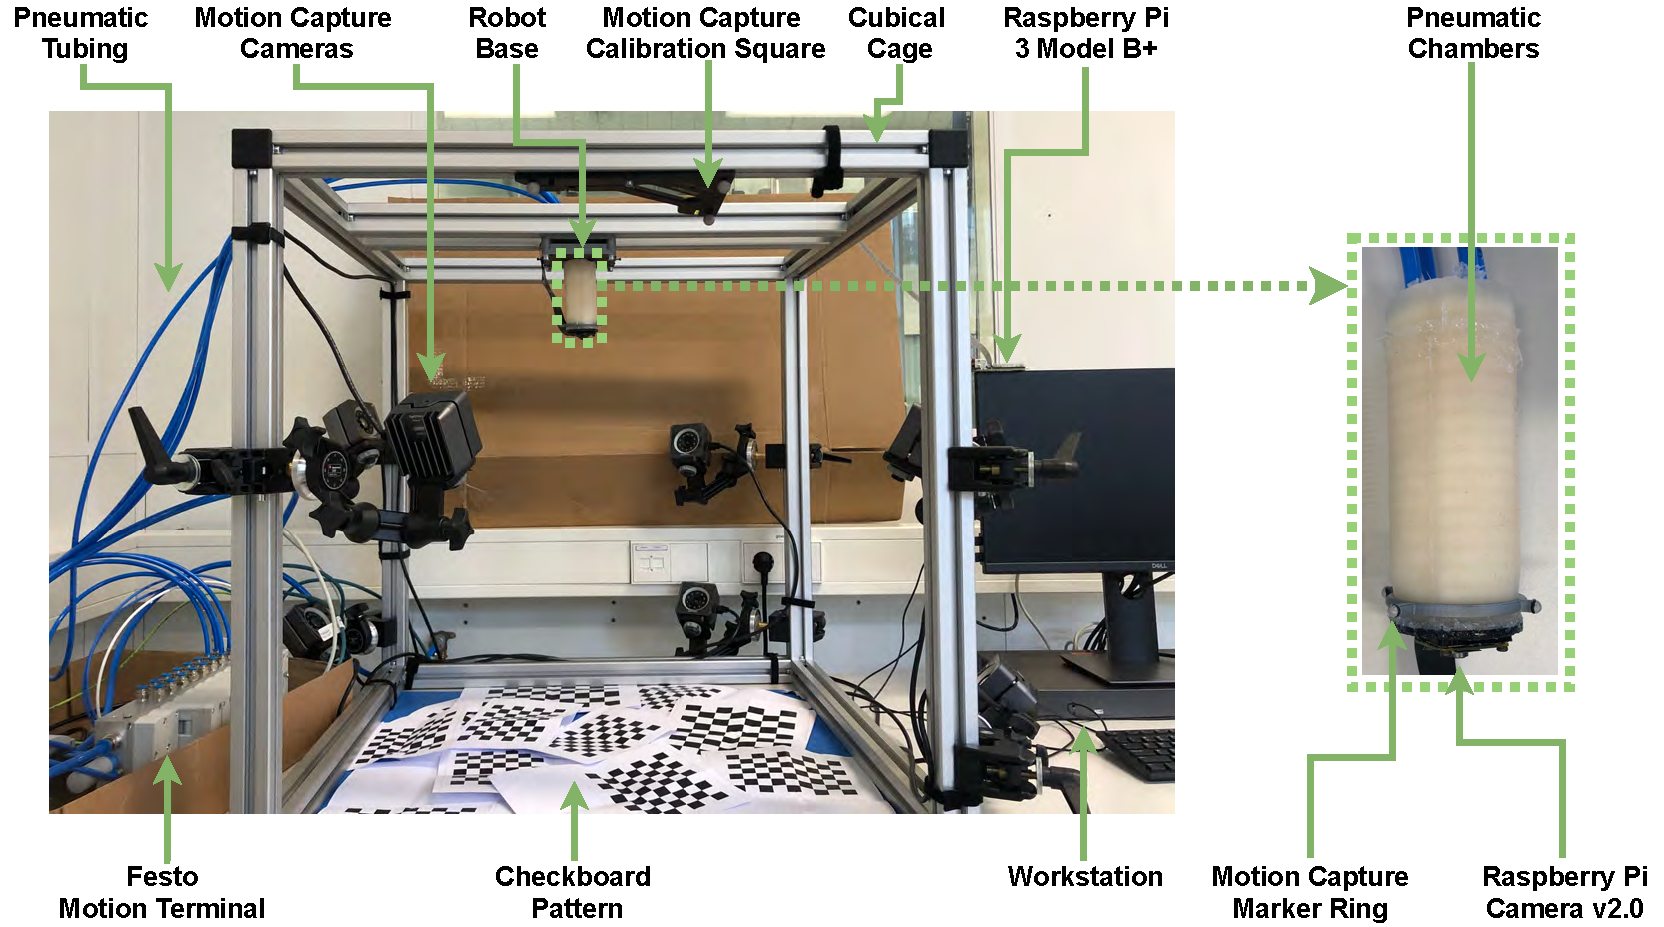
\includegraphics[height=.525\columnwidth]{srslam/figures/graphic_experimental_setup.drawio_v1_compressed.pdf} \label{fig:srslam:experimental_setup}}
     \subfigure[Trajectory 3]{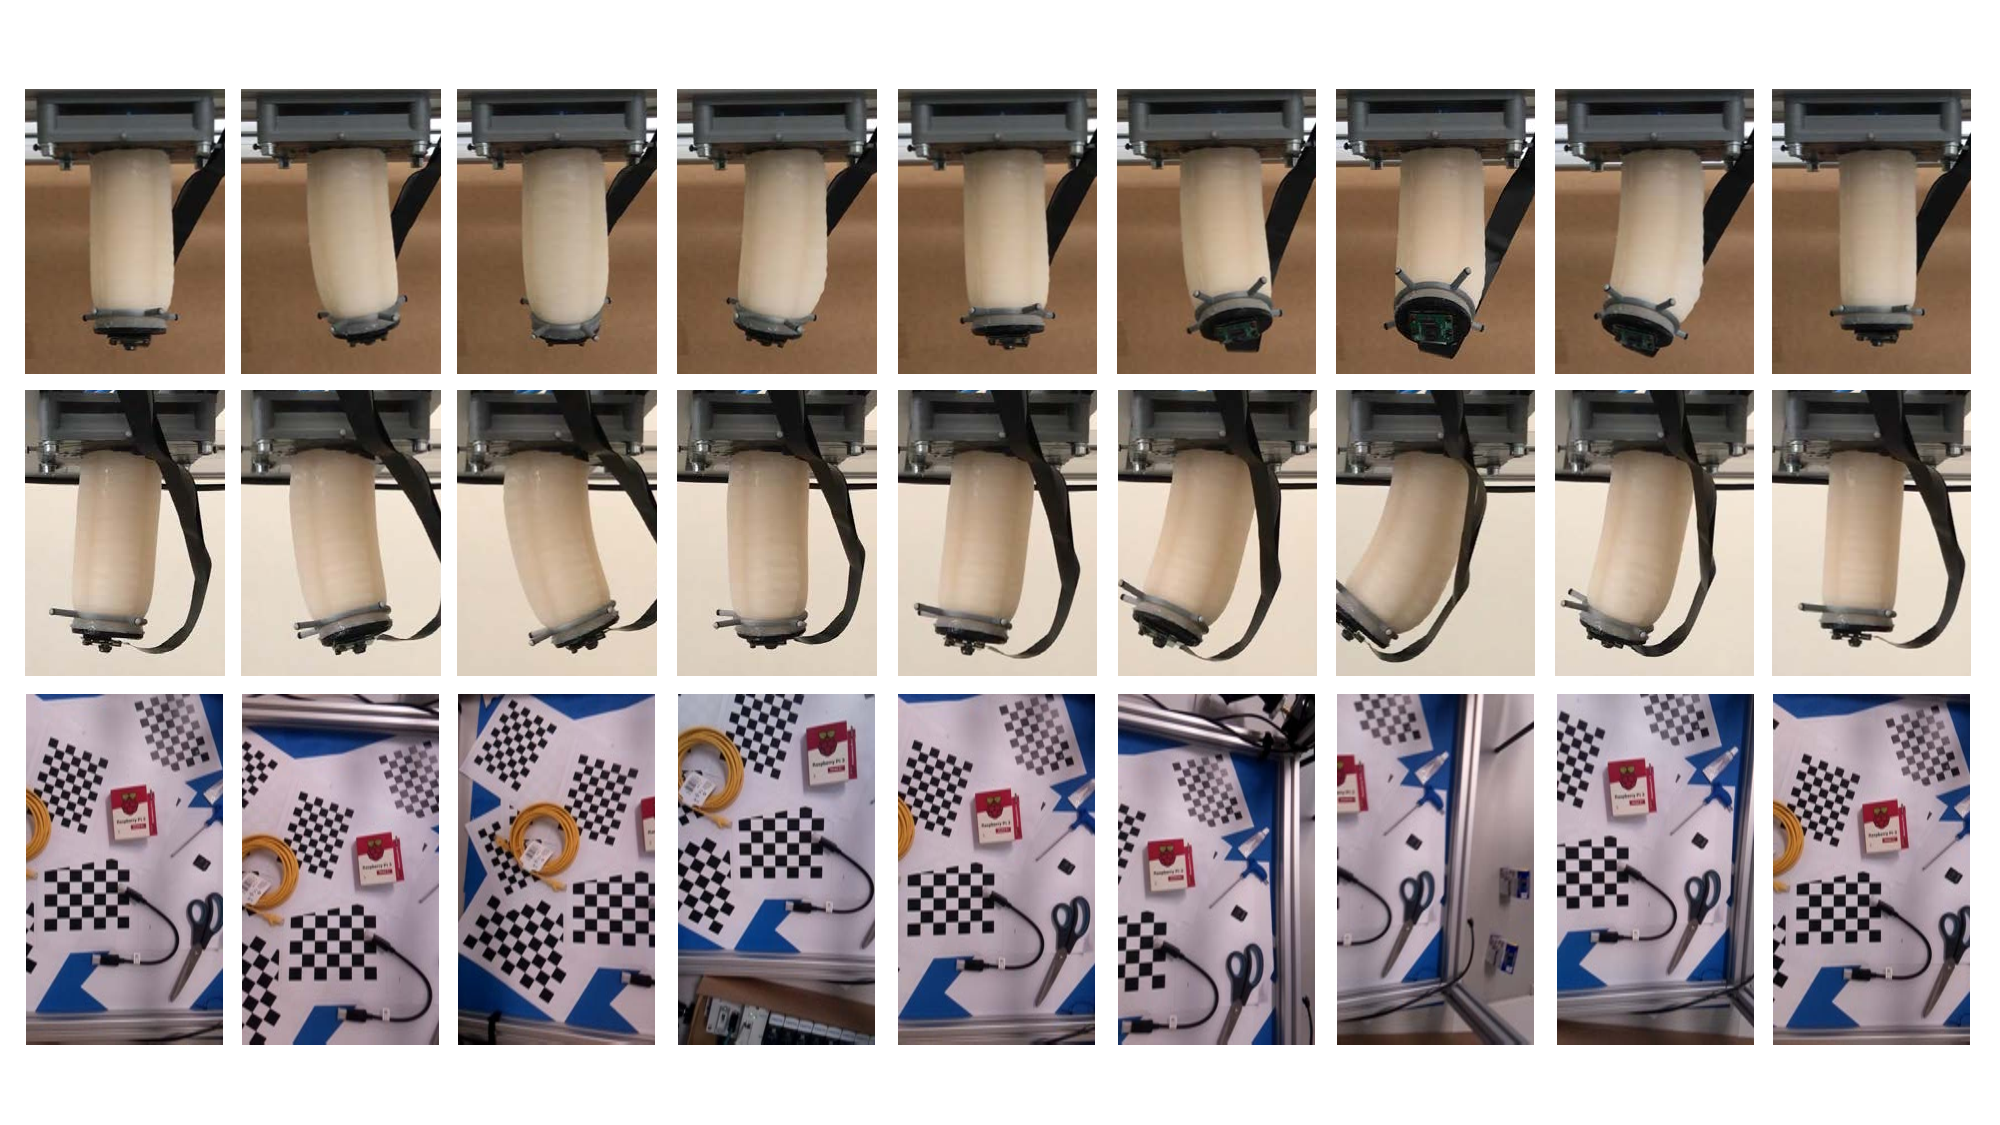
\includegraphics[height=.525\columnwidth]{srslam/figures/graphic_sequences_of_stills_lab_experiment_trajectory_3_compressed.pdf} \label{fig:srslam:graphic_sequences_of_stills_lab_experiment_trajectory_3}}
     \caption{ In Panel (a), a soft robotic segment is mounted to a cage with attached motion capture cameras. The segment is pneumatically actuated by a pressure regulator (Festo Motion Terminal). A Raspberry Pi camera v2.0 is attached to the tip of the segment and, in a straight segment configuration, looks down towards check-board patterns. Panel (b) depicts a sequence of stills showing the robot following trajectory 3 from two different vantage points. The second vantage point differs \SI{90}{\degree} from the first one. The third row displays a few representative frames, as recorded by the camera attached to the tip of the segment.}
\end{figure*}

\subsection{Experimental Setup}
% Segment and manufacturing
We show the experimental setup in Figure~\ref{fig:srslam:experimental_setup}.
We consider a soft robotic silicone segment consisting of four independently inflatable cavities. The segment has a cylindrical shape with a length $L_{0,1}$ of \SI{11}{cm} and a radius $d_1$ of \SI{21}{mm}. 
% We follow the fabrication procedure by \citet{marchese2015recipe} by casting Silicone into 3D-printed molds and block any silicon-flow into the air chambers with bees wax.
A 3D-printed ring with four motion capture markers is located near the tip of the segment.
%
% Camera and its attachment to the segment
We mount a Raspberry Pi camera module v2.0 to the tip of the segment.
This camera has a \SI{8}{MP} sensor and records frames at a sampling rate of \SI{30}{Hz} and a resolution of 1080p.
The focal length is \SI{3.04}{mm} and the field of view is $\SI{62.2}{\degree} \times \SI{48.8}{\degree}$.
The camera module is attached to a Raspberry Pi 3B+ single-board computer, which saves the frames for later processing by the ORB-SLAM~\citep{mur2017orb} algorithm.
The camera is screwed onto a custom 3D-printed holder, which in turn is glued with the tip plane of the segment.
%
% Actuation motion terminal, communication, commanding of pressures
The segment with its four air chambers is actuated with a proportional pressure regulator.
Tubing attached to the base of the segment connects each chamber with the assigned pneumatic valve of the pressure regulator.
%
% We apply a constant offset pressure $p_0$ to all chambers in straight configuration and subsequently synchronously increase the pressure $p_1$ in one chamber by $f_{\mathrm{p},x}$ and decrease the pressure in the opposite chamber $p_2$ by $f_{\mathrm{p},x}$ accordingly to cause a bending of the segment, in this case in x-direction.
% \begin{equation}
% \begin{split}
%     p_1 = p_0 - f_{\mathrm{p},x} \qquad p_2 = p_0 + f_{\mathrm{p},x}\\
%     p_3 = p_0 - f_{\mathrm{p},y} \qquad p_4 = p_0 + f_{\mathrm{p},y}
% \end{split}
% \end{equation}
% We map the desired configuration $\Delta_{x,1}$ and $\Delta_{y,1}$ given by the trajectories defined in \eqref{eq:srslam:trajectory_parametrization} in linear approximation to the commanded pressures
% \begin{equation}
%     f_{\mathrm{p},x} = a_x \; \Delta_{x,1} 
%     \qquad
%     f_{\mathrm{p},y} = a_y \; \Delta_{y,1}
%     \qquad
%     p_0 = a_{\delta L} \; \delta L_1
% \end{equation}
% where the proportional factors $a_{x}$, $a_{y}$ and $a_{\delta L}$ are experimentally determined and an elongation of the segment is reached through an increase in the offset pressure $p_0$.
% The pressure in each chamber is regulated by a Festo Motion Terminal using a factory-tuned PID controller.
% The commanded valve pressures are relayed via Modbus / TCP from our lab workstation to the Motion Terminal at a frequency of approximately \SI{10}{Hz}.
%
% Cage and environment
The segment is attached in an up-side-down configuration to the top plane of a cubical cage of \SI{750}{mm} side length. For a straight segment, the camera is facing downwards towards the floor of the cage, which is covered by multiple printed checkerboard patterns.
%
% Motion capture system and cage
We acquire ground-truth pose information of the tip of the segment using an Optitrack motion capture system. %, consisting of eight PrimeX 13 cameras mounted to the previously mentioned cubic cage. 
The ground-truth poses of the tip of the segment are recorded at \SI{30}{Hz}. % analogous to the Raspberry Pi camera frames.
% Additionally, we also record the pose of the base of the segment allowing us to determine a ground-truth coordinate transformation $T_{0}^{1}$ from the base to the tip.
%
% Implementation of PCC projection and calibration sequence
%In contrast to the model we used in simulation, the real-world segment experiences an elongation caused by the application of pressure to the chambers. Accordingly, 
%
We also include the elongation of the segment $\delta L_1$ in the cost function \eqref{eq:srslam:cost_fun} of our optimization.
%
% Calibration sequence
To resemble the calibration sequence from the simulation for the \gls{SLAM} map, we manually move the robot laterally into the x-coordinate direction before fixing it to the cage for the start of the experiments.

\subsection{Results}
Our experimental results reported in Table~\ref{tab:srslam:results_lab_experiments} and visualized for trajectory 3 in Figure~\ref{fig:srslam:experiments_t3_over_time} show translational relative \gls{RMSE} of between \SI{9}{\percent} and \SI{20}{\percent} for the three trajectories before optimization. 
The orientation of the z-axis of the tip is estimated with a mean error of approximately \SI{0.075}{\radian}.
The translational error is improved to between \SI{5}{\percent} and \SI{9}{\percent} after projection into the \gls{PCC}-kinematics. 
The optimization also slightly improves the rotational \gls{RMSE} by \SI{4}{\percent} to \SI{10}{\percent} relative to naive \gls{SLAM}.

The experimental results of the \gls{SLAM} algorithm are coherent with the simulations, as the small segment length (\SI{11}{cm}) used in the experiments increases the translational errors, as shown similarly in the simulations for a robot of length \SI{15}{cm}.
Even though the translational error is greatly reduced through optimization, it is still significantly higher than in simulation. Two reasons for this difference could be that a) the segment in the simulation was modeled as in-extensible, while the real robot segment is extended via pneumatic pressurization, which introduces additional errors by \gls{SLAM} not accurately estimating the elongation movement and b) the real robot does not perfectly behave according to the \gls{CC} approximation as the simulated robot does.

% \begin{table}
% \centering
% \caption{ \textcolor{orange}{OLD RESULTS: }oReal-world results before and after optimization: the translational errors are stated through a relative \gls{RMSE} and the rotational errors with an absolute \gls{RMSE} taking into account the Frobenius norm of the rotation matrices.}
% \begin{tabular}{lclll}\toprule
% \textbf{Error category} & \textbf{Opt.} & \textbf{Traj. 1} & \textbf{Traj. 2} & \textbf{Traj. 3}\\
% \midrule
% Translation $e_\mathrm{t}$ Eq.~\eqref{eq:srslam:evaluation_translational_error} & No & $\SI{24.8}{\percent}$ & $\SI{21.4}{\percent}$ & $\SI{9.5}{\percent}$ \\
% Translation $e_\mathrm{t}$ Eq.~\eqref{eq:srslam:evaluation_translational_error} & Yes & $\SI{11.4}{\percent}$ & $\SI{13.0}{\percent}$ & $\SI{4.5}{\percent}$ \\
% \midrule
% Rotation $e_\mathrm{R}$ Eq.~\eqref{eq:srslam:evaluation_rotational_error} & No & $0.105$ & $0.131$ & $0.116$ \\
% Rotation $e_\mathrm{R}$ Eq.~\eqref{eq:srslam:evaluation_rotational_error} & Yes & $0.098$ & $0.125$ & $0.112$ \\
% \midrule
% \textcolor{orange}{Rotation $e_{\theta_z}$ Eq.~\eqref{eq:srslam:evaluation_angle_error}} & No & $0.105$ & $0.131$ & $0.116$ \\
% \textcolor{orange}{Rotation $e_{\theta_z}$ Eq.~\eqref{eq:srslam:evaluation_angle_error}} & Yes & $0.098$ & $0.125$ & $0.112$ \\
% \bottomrule
% \end{tabular}
% \label{tab:srslam:results_lab_experiments}
% \end{table}

\begin{table}
\centering
\caption{ Real-world results before and after optimization. The translational errors are stated through a relative \gls{RMSE} as described in \eqref{eq:srslam:evaluation_translational_error}. For rotation, we report both an absolute \gls{RMSE} computed with the Frobenius norm between the rotation matrices as stated in \eqref{eq:srslam:evaluation_rotational_error} and an angle error [rad] for the orientation of the z-axis of the tip of the segment as defined in \eqref{eq:srslam:evaluation_angle_error}. The results are averaged over two trials for each trajectory.}
\begin{tabular}{lclll}\toprule
\textbf{Error category} & \textbf{Opt.} & \textbf{Traj. 1} & \textbf{Traj. 2} & \textbf{Traj. 3}\\
\midrule
Translation $e_\mathrm{t}$ & No & $\SI{20.3}{\percent}$ & $\SI{14.2}{\percent}$ & $\SI{9.1}{\percent}$ \\
Translation $e_\mathrm{t}$ & Yes & $\SI{9.1}{\percent}$ & $\SI{8.9}{\percent}$ & $\SI{5.0}{\percent}$ \\
\midrule
Rotation $e_\mathrm{R}$ & No & $0.145$ & $0.103$ & $0.126$ \\
Rotation $e_\mathrm{R}$ & Yes & $0.130$ & $0.099$ & $0.120$ \\
\midrule
Rotation $e_{\theta_z}$ & No & $\SI{0.079}{\radian}$ & $\SI{0.068}{\radian}$ & $\SI{0.084}{\radian}$ \\
Rotation $e_{\theta_z}$ & Yes & $\SI{0.080}{\radian}$ & $\SI{0.067}{\radian}$ & $\SI{0.084}{\radian}$ \\
\bottomrule
\end{tabular}
\label{tab:srslam:results_lab_experiments}
\end{table}

\begin{figure}[ht]
    \centering
    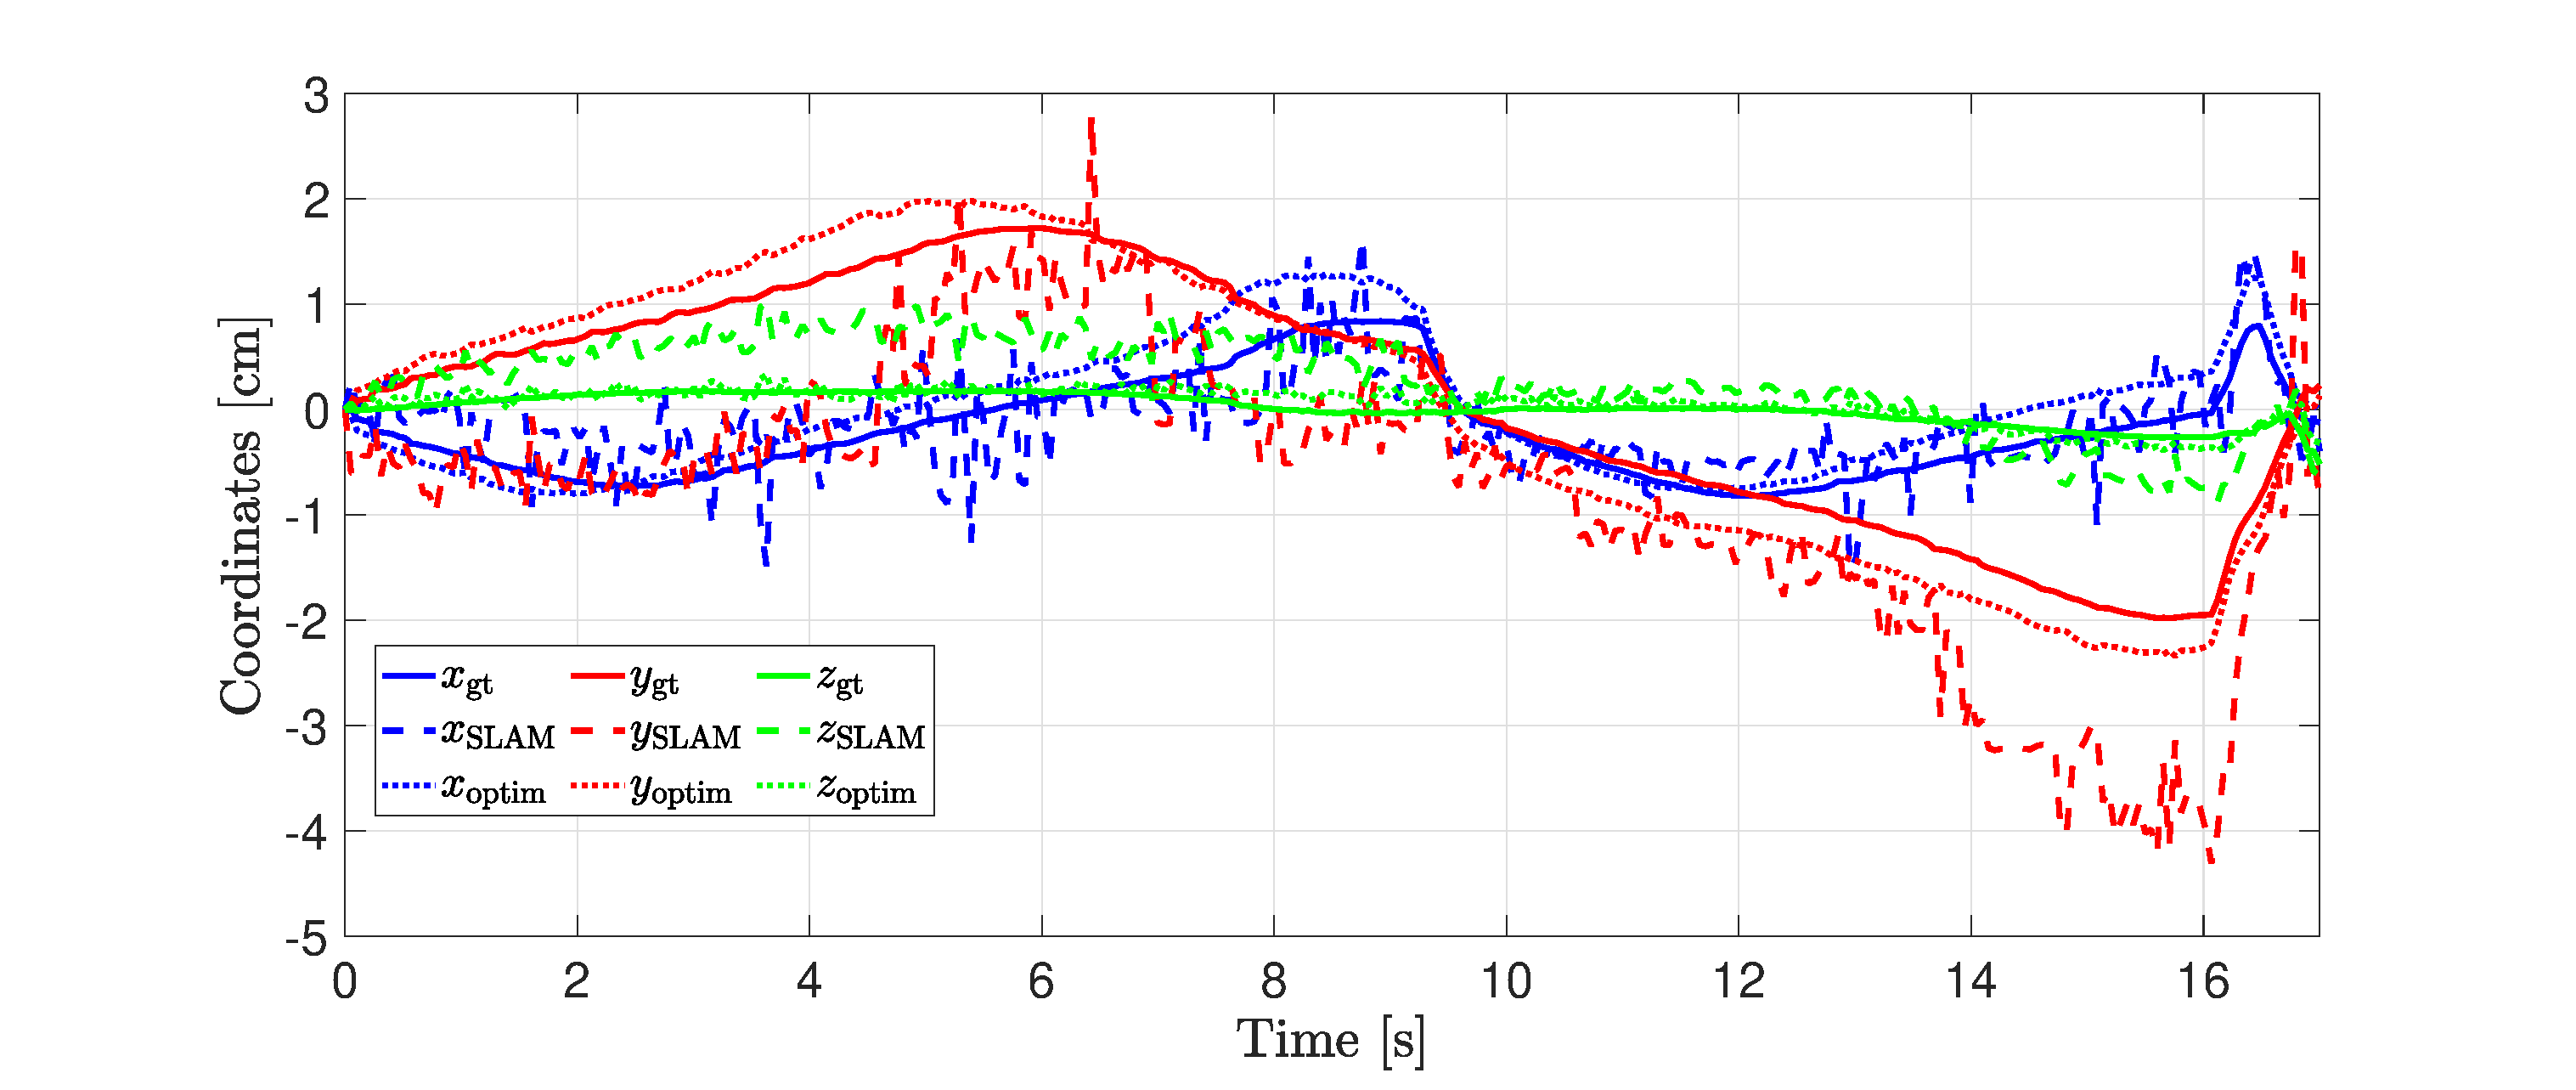
\includegraphics[width=0.9\columnwidth, trim={2cm 1.2cm 2cm 0}]{srslam/figures/vtem28_t3_coordinates.eps}\\
    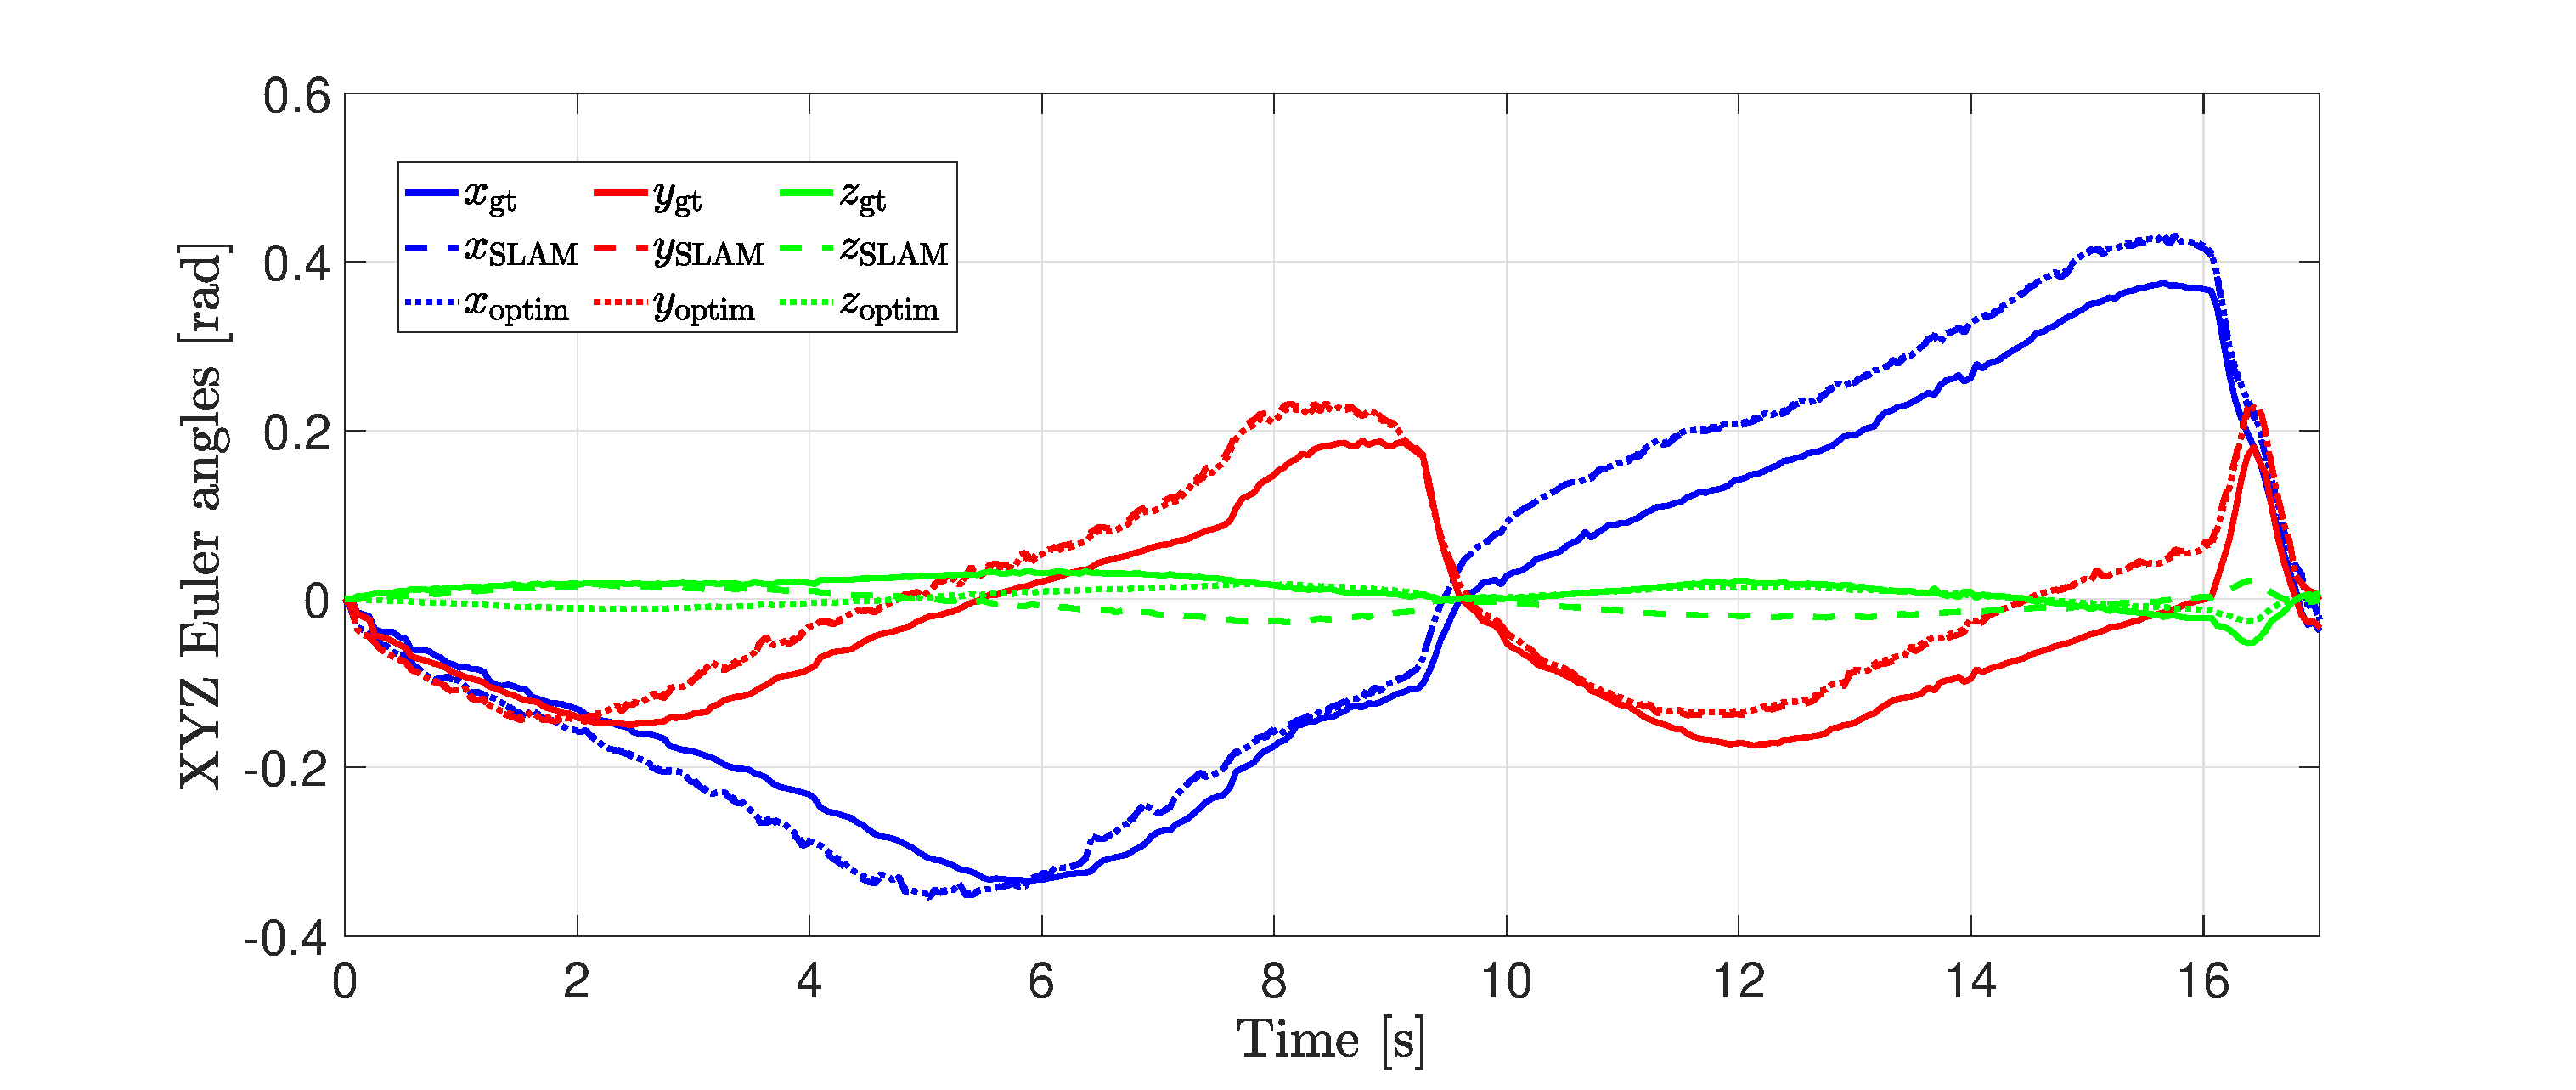
\includegraphics[width=0.9\columnwidth, trim={2cm 0 2cm 1.2cm}]{srslam/figures/vtem28_t3_angles.eps}
    \caption{ Experimental results for trajectory 3. Comparison between ground-truth (solid line), \gls{SLAM} (dashed line), and optimized through projection into \gls{PCC} kinematics (dotted line) for translation and orientation estimates.}
    \label{fig:srslam:experiments_t3_over_time}
\end{figure}


\section{Conclusion}
\label{sec:srslam:conclusions}

This paper investigated using a monocular camera in shape sensing of continuum soft robots, with the ultimate goal of implementing precise and reliable estimations at the cost of introducing small rigid parts into the hardware design. The contribution of this paper has been twofold. First, we proposed to use monocular SLAM with a soft robot. Second, we propose a regularization of the estimation based on a nonlinear projection in the manifold of admitted configuration. A nonlinear optimization implements the latter based on the kinematic model of the robot. We have performed extensive simulations with rendered images in Blender and lab experiments with a single segment soft robot. The nonlinear optimization based on the robot's kinematic model led to a significant improvement in translations and a marginal improvement in rotations. 
Future work will focus on extending the experimental validation of the method to multiple segments and cameras, bettering the SLAM by feeding back the kinematic projection in its state and using this estimation to implement closed-loop control.
While we conducted our experiments in a lab environment under ideal conditions with the camera pointed at checkerboard patterns thus resulting in plenty of image features for \gls{SLAM} to track, future work should investigate whether deployment environments for soft robots would be sufficiently feature-rich for the use of our proposed method.

\section*{Afterword}
This chapter demonstrated how inexpensive commercialized monocular cameras can be effectively used together with established \gls{SLAM} algorithms and kinematic models (e.g., \gls{PCC}) to achieve shape sensing for soft robots. One of the main advantages of this solution is that all necessary components are readily available - either commercially or even via open source. 
% Sharing the same vision, recent work by \citet{caroleo2025soft} combines commercial miniature \gls{TOF} sensors mounted to the tip of a segment with a particle filter for estimating the end-effector pose.
Sharing the same vision, recent work by \citet{caroleo2025soft} integrates commercial miniature \gls{TOF} sensors mounted at the segment tip with a particle filter to estimate the end-effector pose by considering the deviation from a known map of the environment.

However, the approach presented in this chapter also has some drawbacks: 
i) Firstly, while cameras have been significantly miniaturized in recent years, the requirement for them to have a clear, unobstructed view of the environment necessitates the inclusion of a rigid component on the surface of the soft robot, which we generally prefer to avoid for safety reasons. 
Secondly, ii), the performance of \gls{SLAM} algorithms is affected in environments with limited visually distinguishable features.
Finally, iii) high-dimensional perceptive data such as images are generally computationally expensive to process, leading to higher computational requirements and/or relatively low sampling rates of the shape-sensing information.
Therefore, we present in Chapter~\ref{chp:promasens} an alternative shape-sensing approach based on magnetic sensors. The necessary magnets and magnetic sensors can be deeply embedded into the soft robot body, thus allowing us to keep the robot surface entirely soft and compliant. Furthermore, the sensory data is several orders of magnitude lower dimensional, and thus, its processing is potentially much less computationally demanding.
\chapter{Modeling of Handed Shearing Auxetics (HSA) Robots}
\label{chp:hsamodel}

\begin{foreword}
    Novel soft robots based on \glspl{HSA} show great promise by integrating multiple \gls{DOF} in a compact form. Their parallel nature promises a larger payload capacity while preserving compliance. Notably, they represent a paradigm shift in the soft robotics domain by i) establishing compliance through their metamaterial structure rather than material softness and ii) transmitting actuation through their elasticity with the auxetic metamaterial instead of directly applying forces and torques into the desired directions of deformation.
    However, despite the extensive literature on their design, fabrication, and integration of sensing, the absence of kinematic and dynamic models hinders their widespread adoption. These models are crucial for developing accurate simulators and effective model-based controllers.
    This chapter addresses this gap by demonstrating how kinematic (Section~\ref{sec:hsamodel:hsa_rod_kinematics}) and dynamical (Section~\ref{sec:hsamodel:hsa_robot_simulation}) models can be derived for general 3D motion scenarios. Furthermore, we present in Section~\ref{sec:hsamodel:planar_hsa_robot_model} low-dimensional kinematical parametrizations and a control-oriented Euler-Lagrangian model tailored explicitly to planar \gls{HSA} robot motions.
    We follow here a strategy of exploiting the vast and well-grounded literature on control-oriented modeling of rigid robotic manipulators and augment them with a specialized kinematic model based on the \gls{PCS} parametrization and a nonlinear, actuation-dependent elastic model.
\end{foreword}

\blfootnote{This chapter is partly based on 
\begin{itemize}
    \item[\faFileTextO] ~\emph{\textbf{M. Stölzle}, L. Chin, R. L. Truby, D. Rus, and C. Della Santina (2023, April). Modeling Handed Shearing Auxetics: Selective Piecewise Constant Strain Kinematics and Dynamic Simulation. In 2023 IEEE International Conference on Soft Robotics (RoboSoft) (pp. 1-8). IEEE}~\citep{stolzle2023modelling}.
    \item[\faFileTextO] ~\emph{\textbf{M. Stölzle}, D. Rus, and C. Della Santina (2023, December). An Experimental Study of Model-based Control for Planar Handed Shearing Auxetics Robots. In Experimental Robotics: The 18th International Symposium. Springer}~\citep{stolzle2024experimental}.
\end{itemize}
}


\pagebreak

\begin{abstract}
    Electrically-actuated continuum soft robots based on \glspl{HSA} promise rapid actuation capabilities while preserving structural compliance. However, the foundational models of these novel actuators required for precise control strategies are missing. This chapter proposes two key components extending the \glsxtrfull{DCM} to allow for modeling \glspl{HSA}. First, we propose a mechanism for incorporating the auxetic trajectory into \gls{DCM} dynamical simulations. We also implement this extension as a plugin for the Elastica simulator. Second, we introduce a \gls{SPCS} kinematic parameterization that can describe an \gls{HSA} rod's shape with fewer configuration variables. 
    Subsequently, based on the augmented \gls{DCM} model, we devise a low-dimensional kinematic and a control-oriented dynamical model for planar \gls{HSA} robots.
    We verify all theoretical contributions experimentally. The \gls{HSA} robot simulator is used to replicate experimental data of the mechanical characterization of HSA rods. For the kinematic description of the \gls{HSA} rods, we attach motion capture markers at various points to a parallel HSA robot and find that the shape of the \glspl{HSA} can be kinematically represented with an average accuracy of \SI{0.3}{mm} for positions and \SI{0.07}{rad} for orientations.
    Finally, the identified Euler-Lagrangian model for planar \gls{HSA} robots exhibits exceptional accuracy at predicting future system states over a horizon of more than \SI{4}{s}.
\end{abstract}

%% Start the actual chapter on a new page.
\newpage

\section{Introduction}\label{sec:hsamodel:introduction}

% Continuum soft robots promise natural compliance and safe interaction with humans, thanks to their invertebrate-inspired bodies~\citep{della2020softencyclopedia}. Several actuation technologies for soft robots have been explored in recent years, with the most popular being cable-driven and pneumatic actuation~\citep{zaidi2021actuation}.
% Although pneumatically-driven soft robots have been successfully used~\citep{falkenhahn2015dynamic, franco2021position, zaidi2021actuation}, their speed is rather slow and their pneumatic actuation cannot generate twisting thus limiting their Degrees of Freedom (DoF) in task space.
% Cable-driven soft robots generate a pulling force with electric motors using a tendon attached to a soft structure, relying on the elasticity of the system to generate a motion.
%While similarly electrically actuated, 

\dropcap{R}obots based on Handed Shearing Auxetics (HSA) are a recent development in the soft robotics field~\citep{chin2018compliant, truby2021recipe, zhang2022vision, lipton2018handedness, chin2019automated}, which directly transform applied motor torques into complex motion primitives.
%
This novel type of actuator is based on an architected metamaterial. The most important characteristic of this cylindrical metamaterial is that twist strains along the handedness of the structure lead to an elongation of the rod, which is also called auxetic trajectory~\citep{good2022expanding}. 
% These twist strains can be imposed by electric actuation thus enabling fast system responses~\citep{garg2022kinematic}. 
An \gls{HSA} robot combines multiple \glspl{HSA} of different handedness with a platform constraining the movement of the distal ends in the fashion of a soft parallel manipulator. 
Differential elongation of the rods enables complex motion primitives such as elongation, bending, and twisting~\citep{chin2018compliant}, which can be seen in Fig.~\ref{fig:hsamodel:motion_primitives}. % lipton2018handedness
\gls{HSA} robots are particularly difficult to model and control as the forces and torques causing the evolution of the system are not directly produced by the actuator, but instead are intrinsically generated as an effect of the modified cell state of the metamaterial and of the interaction forces coming from the parallel arrangement.

\begin{figure}
    \centering
    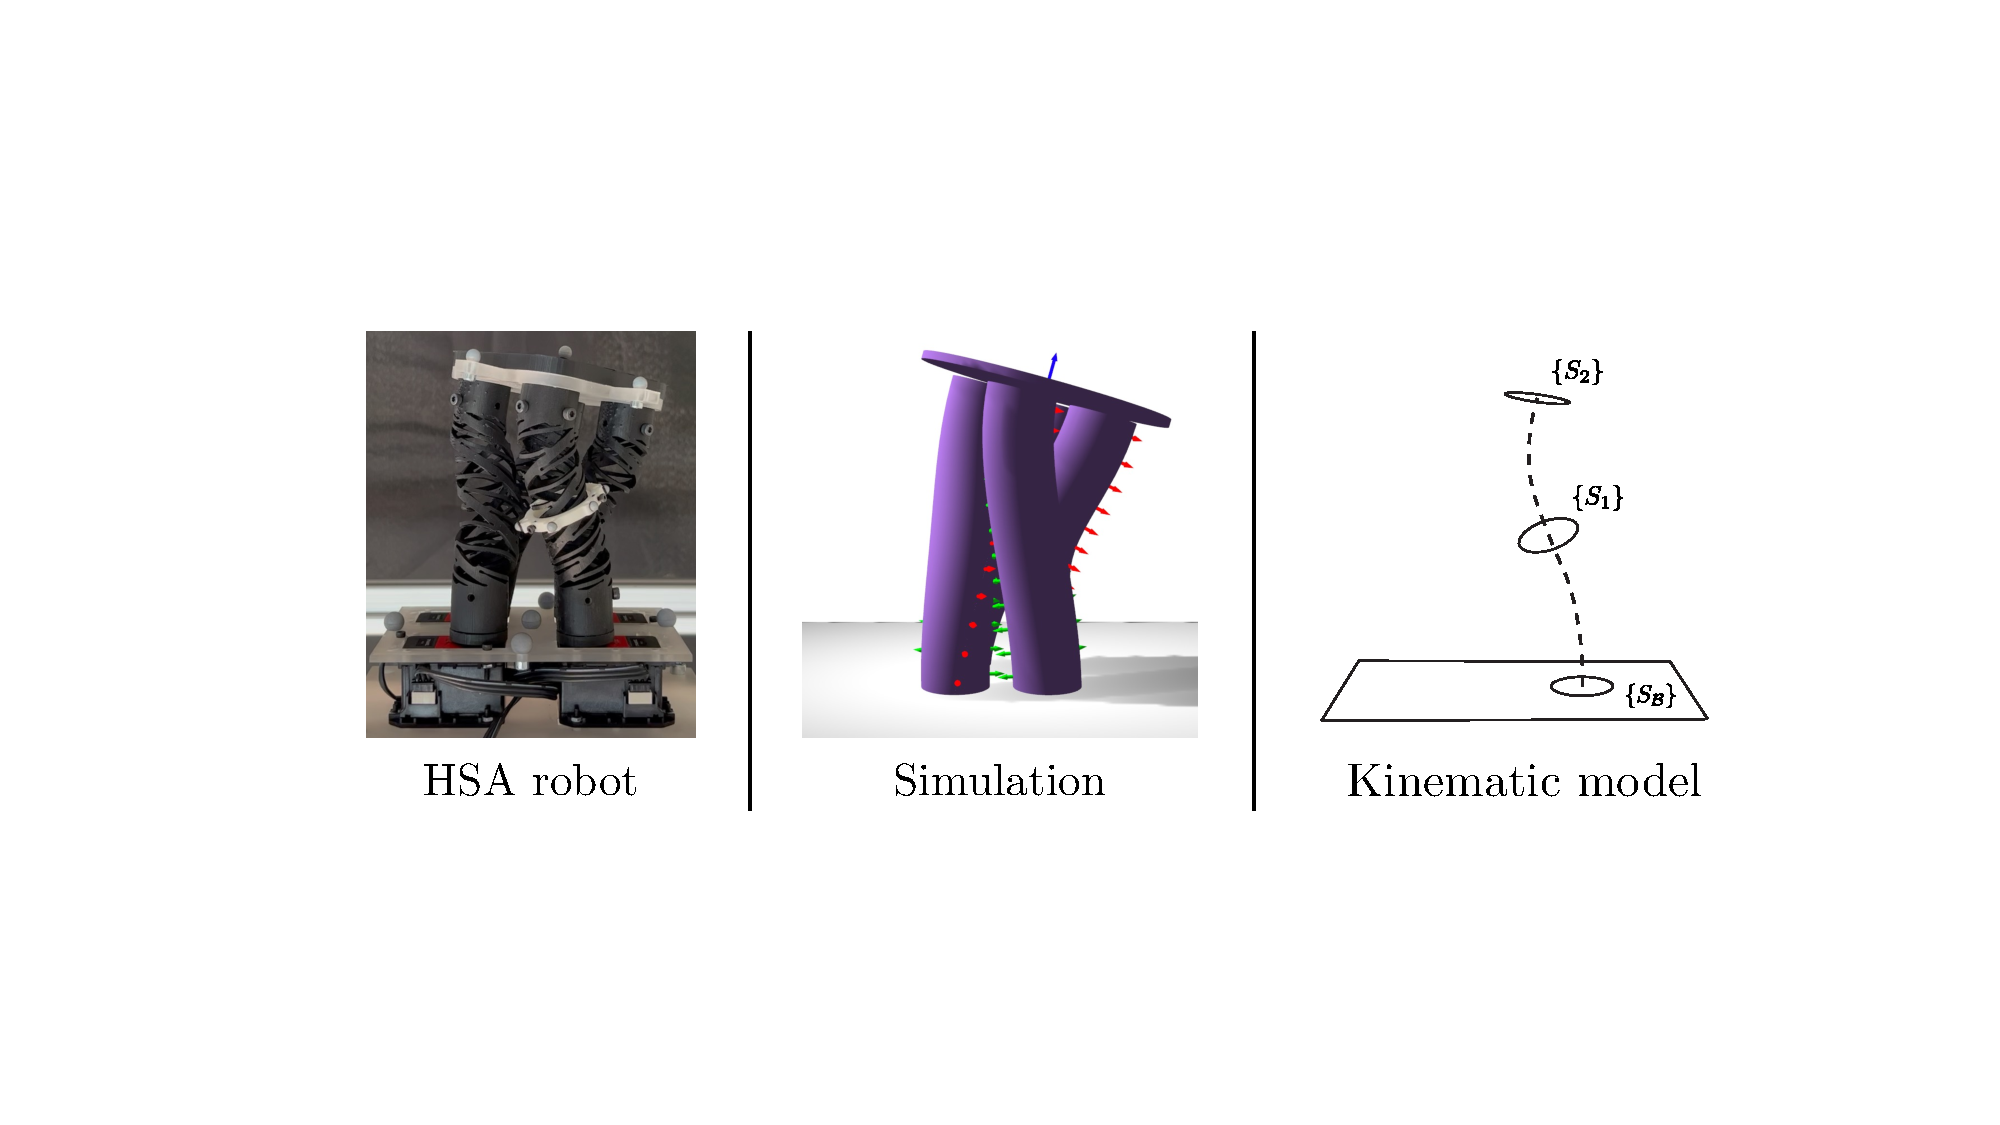
\includegraphics[width=0.72\columnwidth]{hsamodel/figures/overview/overview_v2_cropped.pdf}
    \caption{An HSA robot in a twisted state: simulation and schematic of kinematic model of single HSA rod.}
    \label{fig:hsamodel:overview}
\end{figure}

%This twist strain can be imposed by constraining the tip and simultaneously actuating the proximal end of the \glspl{HSA} with electric servo motors thus enabling fast system responses~\citep{garg2022kinematic}. Combining multiple rods (usually four) of different handedness with a platform at the distal end creates a \gls{HSA} robot. Differential elongation of the rods and leveraging the torsional torques by the motors enable complex motion primitives such as elongation, bending, and twisting~\citep{chin2018compliant, lipton2018handedness}, which can be seen in Fig.~\ref{fig:hsamodel:motion_primitives}.

% This novel type of soft robot consists of four pillars of architected metamaterials.
% The important characteristic of each of the cylindrical auxetics is that twist strains following the handedness of the pattern cause an elongation of the rod. 
% Each of these \glspl{HSA} is independently actuated using electric servo motors thus enabling fast system responses~\citep{garg2022kinematic}.

% Although the latest advances in 3D-printing of metamaterials via digital projection lithography~\citep{truby2021recipe} have made the manufacturing of \gls{HSA} robots much easier, the technology is still expensive and in its infancy. This lack of accessibility severely limits the progress on modeling the behaviour of \gls{HSA} robots and control them successfully. Therefore, a fast simulator is a necessity to allow the research community to rapidly prototype new control strategies.
3D-\gls{FEM} based approaches~\citep{farrell2020extension} have proven to be effective in simulating soft parallel structures \citep{vanneste2021enabling} and could be a good candidate for representing the complex behavior of \gls{HSA} robots. However, in this chapter, we strive for a less computationally expensive solution - towards applications in model-based control \citep{della2023model}. For this reason, we look at the framework of the \gls{DCM}. The Cosserat rod theory assumes the slenderness of the object, e.g. that the length is much larger than the radius, and allows for the rod to exhibit all six principal strains. The 1D discretization of the rod along its length dramatically reduces the computational demand compared to \gls{FEM}~\citep{gazzola2018forward}. 
% The main modification compared to the SoA simulators~\citep{naughton2021elastica, mathew2022sorosim} is that we couple the twist strains to the rest length of the rod. 
%
Several works in recent literature have successfully applied this framework to soft robotics \citep{grazioso2019geometrically,sadati2021tmtdyn,armanini2023soft}. Among them, in \gls{PCS}~\citep{renda2018discrete} the continuum dynamics of the Cosserat model is discretized in space by keeping a selection of strains constant along a segment of the continuum. %They all neglect volumetric deformations and focus on the behavior of the central axis~\citep{della2021model}. 
The most popular \gls{PCS} is \gls{PCC}~\citep{webster2010design}, which assumes a sequence of arcs. Functional extensions of \gls{PCS} use continuous function to approximate the strain~\citep{della2019control,renda2020geometric}. %The functional subspace is split into basis functions and weights, which are taken as the configuration of the robot~\citep{della2021model}. 
% Finally, \gls{FEM} models represent the shape of the continuum with a mesh~\citep{grazioso2019geometrically}, therefore not neglecting the volumetric deformations.

\begin{figure*}[hbt]
    \centering
    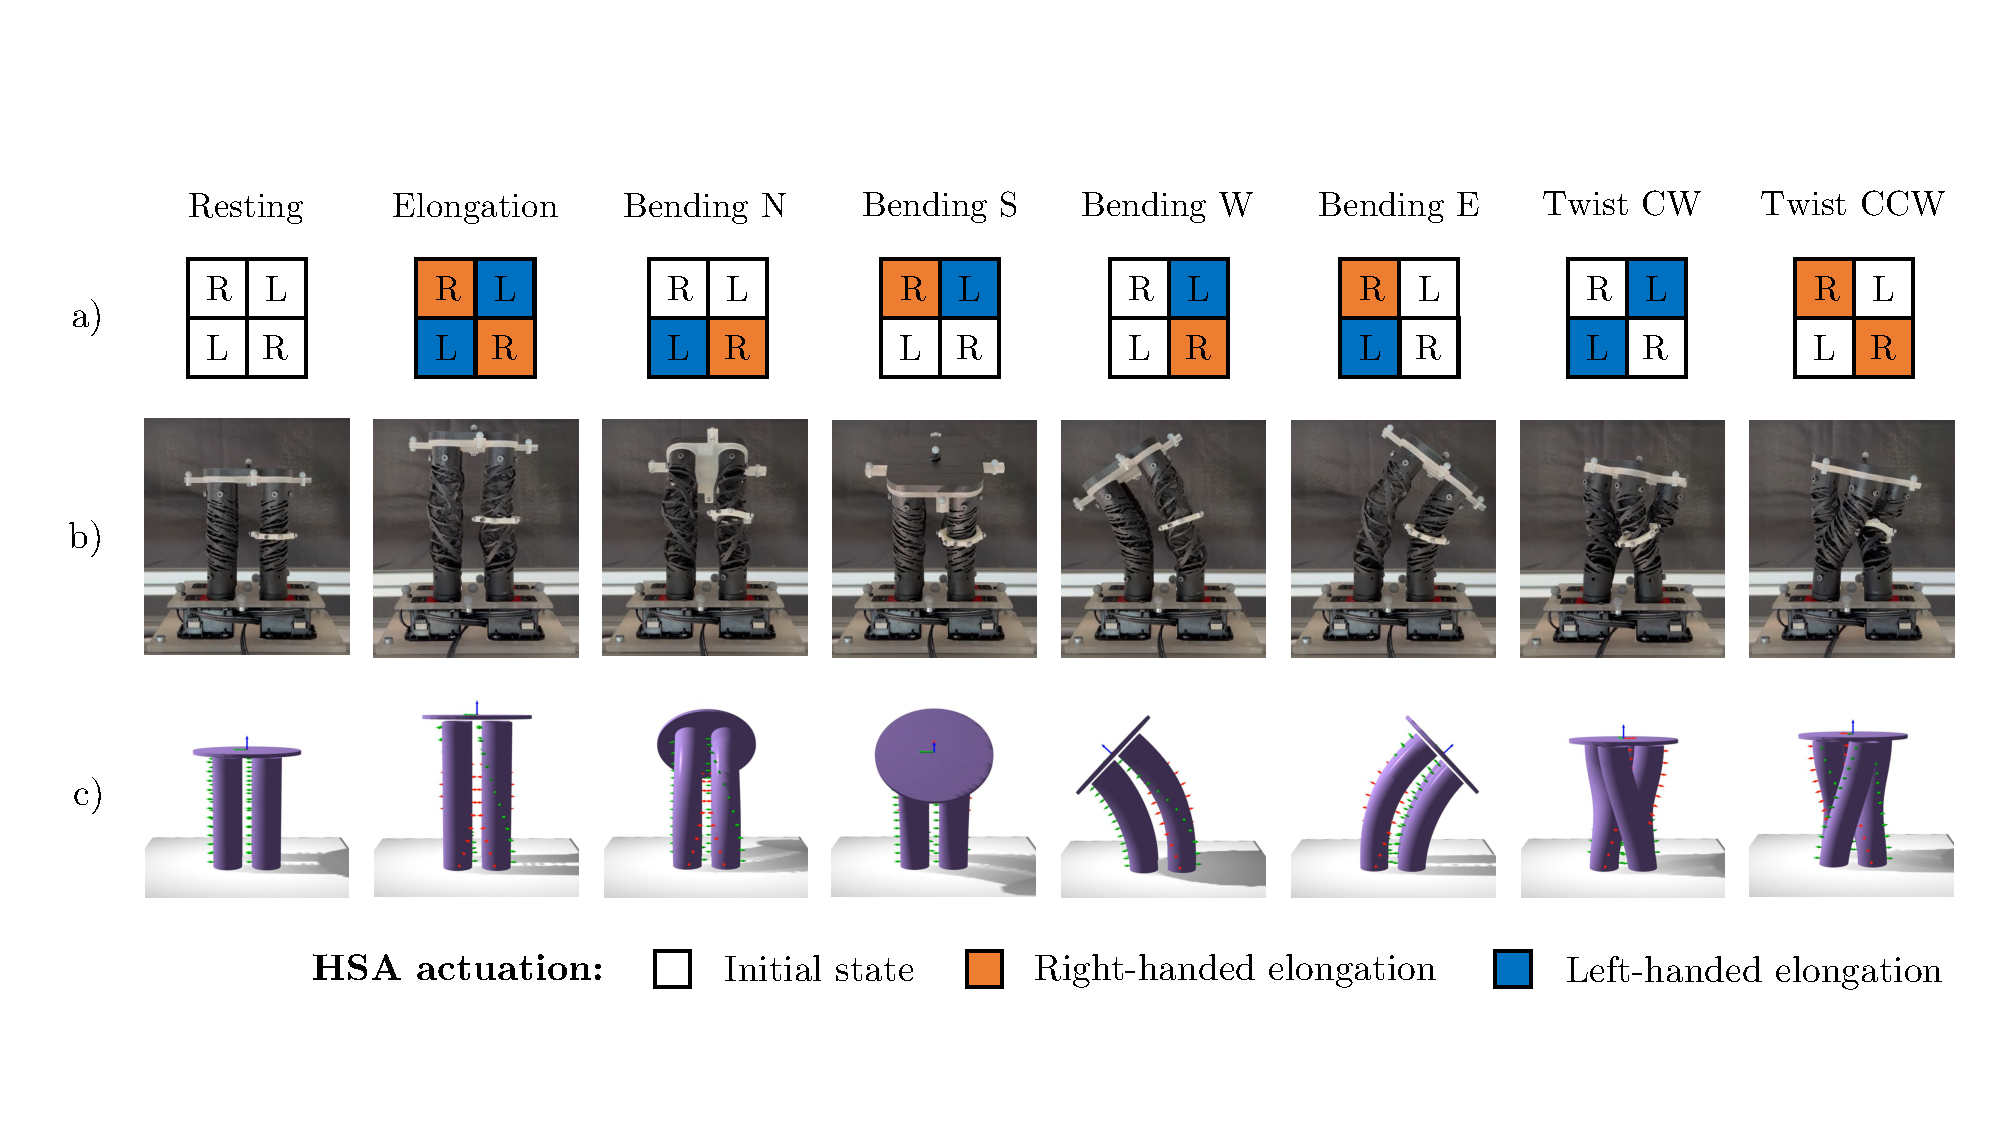
\includegraphics[width=1.0\textwidth]{hsamodel/figures/motion_primitives/motion_primitives_v2_compressed.pdf}
    
    \caption{Motion primitives of Handed Shearing Auxetic (HSA) robots: elongation, bending in the four cardinal directions (e.g., north (N), south (S), west (W), east (E)), and clockwise (CW) and counter-clockwise (CCW) twisting.
    \textbf{First row (a):} depicts the necessary actuation inputs to generate these motion primitives. Pure elongation is achieved by applying the motor torques of the same magnitude but in opposite directions to the left-handed (L) and right-handed (R) HSAs. For bending, there exists a delta in the elongation of the rods while the sum of torques is still zero. Last but not least, counter-clockwise twisting is achieved by applying more torque to the right-handed, than to the left-handed HSA rods.
    \textbf{Second row (b):} Snapshots of the experimental platform when actuated according to the above-specified sequence.
    \textbf{Third row (c):} Renderings of simulated steady-states of an HSA robot. It consists of four HSA rods and a platform at the distal end. The red arrows point along the local x-axis, and the green arrows along the local y-axis, respectively. The blue arrow signifies the z-axis of the local frame of the platform.}\label{fig:hsamodel:motion_primitives}
\end{figure*}

However, none of these methods are currently applicable to HSA robots, as they do not embed a mechanism for incorporating the effect of the auxetic trajectory.
%
We are aware of just one work looking into kinematic modeling of HSA robots~\citep{garg2022kinematic}, which, however, models the backbone of the robot with \gls{PCC} instead of modeling the HSAs. As a consequence, the model cannot represent complex behaviors of the module, like the twist in Fig.~\ref{fig:hsamodel:overview}. 

The goal of this chapter is to provide such a mechanism for the general movement of \gls{HSA} robots in 3D-space, to introduce a strategy for further reducing the dimensionality of the model, to derive a control-oriented model for planar \gls{HSA} robots, and to provide extensive experimental validation for all. 
More specifically, our extension to the \gls{DCM} framework couples the twisting strain of the \gls{HSA} rod to its rest length. %The elastic modulus together with the axial strains will then naturally drive the \gls{HSA} towards this rest length.
Additionally, we allow the rigidity of the rod to be modified as a function of the twist strain. %This is necessary as new work on identifying the mechanical characteristics of \glspl{HSA}~\citep{good2022expanding} has shown that the spring constant increases with the twist strains.
We have implemented this mechanism as a plugin for Elastica~\citep{naughton2021elastica}, which we provide open source\footnote{\url{https://github.com/tud-phi/HSA-PyElastica}}. 
% This results in a compact dynamic model that we test experimentally.
% Several SoA simulators simulators~\citep{naughton2021elastica, mathew2022sorosim} rely on this discretized Cosserat rod theory.

We then use a combination of \gls{CS} and \glspl{PCS}~\citep{renda2018discrete} to describe the shape of \gls{HSA} rods, which we call a \gls{SPCS} model: while some strains, such as twist \& stretch, are mostly constant over the length of the entire \gls{HSA}, other strains such as bend \& shear significantly vary and are thus captured in a piecewise parametrization. 
Our results show that a kinematic parametrization with $11$ Degrees of Freedom (DoF) is sufficient to capture the shape of \glspl{HSA}.
Compared to the \gls{DCM} strategy used for simulating \glspl{HSA}, we have, therefore, significantly reduced the DoF of the kinematics.
We provide an open-source implementation of this kinematic model in JAX\footnote{\scriptsize \url{https://github.com/tud-phi/jax-spcs-kinematics}}.
% Furthermore, we propose a Selective Piecewise Constant Strain (SPCS) kinematic model to describe the full 3D deformation of a single \gls{HSA} rod with a dramatically reduced number of states (compared to the \gls{DCM} strategy).

This kinematic model could then be used to parametrize the deformation of each limb in the parallel \gls{HSA} rod.
However, this would require the enforcement of kinematic constraints~\cite {armanini2021discrete}, which can be algorithmically and computationally challenging.
We propose to avoid this complexity in the planar case, by natively incorporating the kinematic constraints into the model. In particular, we 
defining the \gls{CS} of a virtual backbone in the center of the robot to be our configuration variable.
Finally, we derive the system dynamics of a planar \gls{HSA} robot in Euler-Lagrangian form.

In summary, we contribute to the state of the art in the modeling of soft robots with:
%
\begin{enumerate}
    \item A mechanism for integrating the auxetic trajectory of \glspl{HSA} into the discrete Cosserat rod theory~\citep{gazzola2018forward, mathew2022sorosim}. %Specifically, we modify the rest length of the rod as a function of the twist strain to cause an elongation of the \gls{HSA}.
    \item A plugin for the Elastica simulator~\citep{naughton2021elastica}, which also includes the necessary boundary conditions and joint formulations to simulate \gls{HSA} robots.
    \item A Selective Piecewise Constant Strain (SPCS) kinematic model to parameterize the shape of a single \gls{HSA} rod with a dramatically reduced number of states. %Namely, we combine strain components constant along the entire length with piece-wise constant strains. %This concept allows us to dramatically reduce the dimensionality of the model, which is ideal for control purposes. We verify this model's ability to describe the shape of the rods of an \gls{HSA} robot in both simulation and experimentally.
    \item A closed-form solution for the inverse kinematics of a planar \gls{CS} formulation.
    \item A Euler-Lagrangian dynamical model for planar \gls{HSA} robots.
\end{enumerate}
% \begin{itemize}
%     \item We infuse the auxetic trajectory into the discretized Cosserat rod theory to build a dynamical simulator of HSA robots and add support for the common mechanical characteristics of \gls{HSA} rods.
%     \item We show that the shape of \gls{HSA} rods can be kinematically described by very few parameters within the \gls{PCS} framework. This twist-aware kinematic model is able to reconstruct the local orientation of the \gls{HSA} rods and is with that also suitable for twisting motion primitives.
%     % \item We propose a kinematic parametrization for \gls{HSA} rods, which are i) able to derive the local orientation of the rod, and ii) also are suitable for the twisting motion primitive of \gls{HSA} robots.
% \end{itemize}
Contributions (1) and (2) are covered in Section~\ref{sec:hsamodel:hsa_robot_simulation}. Subsequently, we introduce the kinematic model from contribution (3) and experimentally verify it in Section~\ref{sec:hsamodel:hsa_rod_kinematics}. The control-oriented model for planar \gls{HSA} robots from contributions (4) and (5) and the experimental validation are presented in Section~\ref{sec:hsamodel:planar_hsa_robot_model}.
\section{Dynamic simulation of HSA robots}\label{sec:hsamodel:hsa_robot_simulation}
We introduce a new concept to enable the simulation of \gls{HSA} robots with the discretized Cosserat rod theory, which is used by many of the SoA simulators of soft continuum robots~\cite{naughton2021elastica, mathew2022sorosim}.
While we provide an implementation of the proposed concept as a plugin to Elastica~\cite{naughton2021elastica}, the same strategy could be used to adapt other simulators such as SoRoSim~\cite{mathew2022sorosim} to \gls{HSA} robots.
% The proposed mechanism couples the rest length of the rods with their twist strains to mirror the auxetic trajectory and modifies the stiffness of the rod as a function to the twist strain to match the known mechanical characteristics of \glspl{HSA}. %~\cite{good2022expanding}.
% We provide an implementation of this strategy through a plugin for the Elastica simulator~\cite{naughton2021elastica}.
% Our simulator is based on a discretized version of the Cosserat rod theory~\cite{renda2018discrete, gazzola2018forward, naughton2021elastica, mathew2022sorosim} and allows the user to simulate the behaviour of a system consisting of $n_\mathrm{HSA}$ rods, each with a handedness $h_j \in \{-1, 1 \}$, and a rigid cylindrical platform constraining all of the \glspl{HSA} at their tips.
%
We give some background on the \gls{DCM} in Section~\ref{sub:hsamodel:hsa_robot_simulation:discretized_cosserat_rod_model}. Then, in \ref{sub:hsamodel:hsa_robot_simulation:auxetic_trajectory}, we propose a mechanism to infuse the auxetic trajectory for a \gls{HSA} into the \gls{DCM} framework. Subsequently, we verify the steady-state behaviour of an \gls{HSA} against the mechanical characteristics in \ref{sub:hsamodel:hsa_robot_simulation:verification_good}. Next, we lay out in \ref{sub:hsamodel:hsa_robot_simulation:hsa_robots} the necessary boundary conditions of the \glspl{HSA} and describe the joint mechanism connecting the platform with the rods. Finally, we explain in Section~\ref{sub:hsamodel:hsa_robot_simulation:motion_primitives} how we were able to reproduce in simulation the main motion primitives of \gls{HSA} robots.

\subsection{Background: Discretized Cosserat-rod model}\label{sub:hsamodel:hsa_robot_simulation:discretized_cosserat_rod_model}
This subsection will introduce the governing equations of the \gls{DCM} following the work by Gazzola et al.~\cite{gazzola2018forward}.
According to the Cosserat rod theory, a slender rod's shape can be purely described by the line along its backbone. % The coordinate $s \in [0,L] \in \mathbb{R}$ can then be used to define a point along the backbone. % arc-length coordinate
The backbone curve is divided into a discrete set of nodes with position $r_i(t) \in \mathbb{R}^3$ for $i \in \{1,\dots,n_\mathrm{v}+1\}$ and $n_\mathrm{v}$ links of orientation $Q_i(t) \in \mathbb{R}^{3 \times 3}$.
Differentiating the position and orientation with respect to time gives the translational and angular velocities $v_i = \frac{\partial r_i}{\partial t} \in \mathbb{R}^3$ and $\omega_{\mathcal{L}}^i \in \mathbb{R}^3$.
% The $\mathcal{L}$ subscript denotes that the quantity lives in the body-convected frame, while all other variables are described in the inertial frame.
Each node has a mass of $m_i$ and the rigid links are modelled to have a second mass moment of inertia $J_i$.
When a rod of unstretched length $\hat{L}$ is at rest, each link has a length of $\hat{l}_i$ and connects two consecutive vertices. 
The circumflex accent will denote quantities in the rest configuration of the rod.
When the rod is in a deformed state, $l$ describes the current edge length and
% In contrast to the Kirchoff-Love theory, which does not allow for shear and extension to occur, the Cosserat rod theory accounts for all six deformation modes. 
the shear and axial strains are considered in the vector $\sigma = \begin{pmatrix} \sigma_x & \sigma_y & \sigma_z \end{pmatrix}^\mathrm{T}$. The curvature vector $\kappa_{\mathcal{L}} = \begin{pmatrix} \kappa_x & \kappa_y & \kappa_z \end{pmatrix}^\mathrm{T}$ captures the bending and twist strains.
All strains are defined with respect to the rest length of the link $\hat{l}_i$ and the dilation factor $e_i = \frac{l_i}{\hat{l}_i}$ denotes the deviation from that rest length.
The shear and stretch stiffness is specified through the diagonal matrix $S = \mathrm{diag}(E I_{xx}, E I_{yy}, G I_{zz}) \in \mathbb{R}^{3 \times 3}$, where $E$, $G$ are the elastic and shear modulus respectively, and $I \in \mathbb{R}^{3 \times 3}$ is the second area moment of inertia. Analogue, the bending and twist rigidity is stored in $B = \mathrm{diag}(B_x, B_y, B_z) \in \mathbb{R}^{3 \times 3}$.
For conciseness, we include below only the equation for the translational accelerations. We refer the interested reader to \cite{gazzola2018forward} for the equation on rotational accelerations and more complimentary details about the \gls{DCM}.
% The translational and rotational accelerations are then given as part of the governing equations as
\begin{align}
    m_i \frac{\partial v_i}{\partial t} =& \Delta^h \left ( \frac{Q_i^\mathrm{T} \hat{S}_i \sigma^i_{\mathcal{L}}}{e_i} \right ) + F_i, \quad i\in \{1,\dots,n_\mathrm{v}+1\},
    %\frac{\hat{J}_i}{e_i} \frac{\partial\omega_{\mathcal{L}}^i}{\partial t} =& \Delta^h \left ( \frac{\hat{B}_i \hat{\kappa}_{\mathcal{L}}^i}{\epsilon^3_i} \right ) + \mathcal{A}^h \left ( \frac{\hat{\kappa}_{\mathcal{L}}^i \times \hat{B}_i \hat{\kappa}^i_{\mathcal{L}}}{\epsilon^3_i} \right )\notag\\
    %&+ (Q_i t_i \times \hat{S}_i \sigma_{\mathcal{L}}^i)\hat{l}_i + \left ( \hat{J}_i \frac{\omega^i_{\mathcal{L}}}{e_i} \right ) \times \ \omega_{\mathcal{L}}^i\notag\\
    % &+\frac{\hat{J}_i \omega^i_{\mathcal{L}}}{e_i^2} \frac{\partial e_i}{\partial t} + \tau_{\mathcal{L}}^i, \quad i=[1,n_\mathrm{v}],
\end{align}
where $F_i \in \mathbb{R}^3$ is the external force acting on the $i$th vertex.
Several quantities are expressed in the Voronoi domain $\mathcal{D}$, in which the length of the region $\mathcal{D}_i$ can be computed as $\mathcal{D}_i = \frac{l_{i+1} + l_i}{2}, i \in [1,n_\mathrm{v}-1]$. Examples are the % Voronoi dilation $\epsilon_i$, 
the Voronoi curvature $\hat{\kappa}_{\mathcal{L}}^i$ over the interior vertices, and the bend twist stiffness matrix $\hat{B}_i$.
$\Delta^h : \{\mathbb{R}^3 \}_N \rightarrow \{ \mathbb{R}^3 \}_{N+1}$ is used as the discrete difference operator.
% where $F_i \in \mathbb{R}^3$ and $\tau^i_{\mathcal{L}} \in \mathbb{R}^3$ are the external force and couple acting on the $i$th vertex and link respectively.
% Several quantities were expressed in the Voronoi domain $\mathcal{D}$, in which the length of the region $\mathcal{D}_i$ can be computed as $\mathcal{D}_i = \frac{l_{i+1} + l_i}{2}, i \in [1,n_\mathrm{v}-1]$. Examples are the Voronoi dilation $\epsilon_i$, the Voronoi curvature $\hat{\kappa}_{\mathcal{L}}^i$ over the interior vertices, and the bend twist stiffness matrix $\hat{B}_i$.
% $\Delta^h : \{\mathbb{R}^3 \}_N \rightarrow \{ \mathbb{R}^3 \}_{N+1}$ is used as the discrete difference operator and $\mathcal{A}^h : \{\mathbb{R}^3 \}_N \rightarrow \{ \mathbb{R}^3 \}_{N+1}$ averages over $\mathcal{D}$ to get the corresponding values in the node domain.

\subsection{Auxetic trajectory}\label{sub:hsamodel:hsa_robot_simulation:auxetic_trajectory}
% We implement several modifications and extension to the Elastica simulator~\cite{gazzola2018forward} to allow for realistic simulation of \glspl{HSA}.
We propose several adjustments to the standard definition of the \gls{DCM} to allow for realistic simulation of \glspl{HSA}.
The main assumption behind the proposed concept is that twist strains agreeing with the handedness of the rod will modify the internal angle between the auxetic pattern cells and with that also change the system characteristics such spring constant, blocked force, etc.

Most importantly, we introduce a distinction between the the printed, initial, length of the \gls{HSA} $\bar{L}$ and the rest length of the rod $\hat{L}$. 
This allows us to mirror the auxetic trajectory, as the minimum energy length is increased with applied twist angles / strains~\cite{good2022expanding}.
Similar to the \textsc{hat} accent, which denotes rest quantities, the \textsc{bar} accent will point out quantities of the \gls{HSA} in the initial / printed state.
%As an example, when the twist strain $\kappa_{\mathcal{L},z}$ is zero, $\bar{L} = \hat{L}$. However when twist strains are present, 
We propose to linearly scale the edge rest length $\hat{l}_i$ with the twist strain $\kappa_{\mathcal{L},z}^i$:
\begin{align}
    \hat{l}_i &= (1 + \varepsilon_i) \, \bar{l} \quad i\in \{1,\dots,n_\mathrm{v}+1\},\\
  \varepsilon_i &= \max \left (\min \left (h \: C_{\varepsilon} \, \mathcal{A}^h(\kappa_{\mathcal{L},z}^i),\varepsilon_\mathrm{max} \right ), \varepsilon_\mathrm{min} \right ).
\end{align}
In this expression, the twist strain $\kappa_{\mathcal{L},z}^i$ is elevated from the Voronoi to the vertex domain with the averaging operator $\mathcal{A}^h : \{\mathbb{R}^3 \}_N \rightarrow \{ \mathbb{R}^3 \}_{N+1}$. $h \in \{ -1, 1 \}$ is the handedness of the rod. Right is defined as the positive, and left as the negative handedness.
$C_{\varepsilon}$ is the extension factor, which needs to be tuned with respect to the chosen auxetic pattern.
The minimum and maximum extension $\varepsilon_\mathrm{min}$, $\varepsilon_\mathrm{max}$ are the limits of the auxetic trajectory and depend on the \gls{HSA} type: for example closed \glspl{HSA} can only exhibit positive elongations~\cite{good2022expanding}. % Contrarily, semi-open \glspl{HSA} can both contract and elongate~\cite{good2022expanding}.
After the rest length is adjusted, the axial stiffness of the rod will guide the current edge length $l_i$ towards the (target) edge rest length. % $\hat{l}_i \neq \bar{l}_i$
% This strategy allows us to keep the axial deformability in tact, while adjusting the length of the rod according to the auxetic trajectory.
Furthermore, we recall the definition of bend / twist strains: $\kappa_{\mathcal{L}}^i = \frac{\log(Q_{i+1} \: Q_i^\mathrm{T})}{\hat{\mathcal{D}}_i}$. 
% As the rest length is changed while traversing the auxetic trajectory, the Voronoi rest length $\hat{\mathcal{D}}_i$ and therefore the twist strain $\kappa_{\mathcal{L}}^i$ would change as well. 
To keep the twist strain constant across the entire auxetic trajectory, we define the twist strain with respect to the initial Voronoi length $\bar{\mathcal{D}}_i = \frac{\bar{l}_{i+1} - \bar{l}_i}{2}$:
\begin{equation}
    \kappa_{\mathcal{L},z}^i = \frac{\log(Q_{i+1} \: Q_i^\mathrm{T})}{\bar{\mathcal{D}}_i}, \quad i\in \{1,\dots,n_\mathrm{v}+1\}
\end{equation}

\begin{table}[hbt]
\centering
\caption{Parameters of simulated HSA rods in Section~\ref{sub:hsamodel:hsa_robot_simulation:verification_good} for various number of HSA row tilings $n_\mathrm{rows}$. Row tilings represent the number of vertically stacked unit cells~\cite{good2022expanding}. The rest length $\hat{L}$ and the elastic modulus $E$ are a linear function of the twist strain $\kappa_z$. $B_z$ represents the twist rigidity.}
\begin{tabular}{c ccc}\toprule
$n_\mathrm{rows}$ & $\hat{L} \, [\si{mm}]$ & $E \, [\si{kPa}]$ & $B_z \, [\si{Nm^2 \per rad}]$\\
\midrule
$4$ & $75 \, (1 + 3.04 \: \kappa_z)$ & $576.9 + 36.1 \: \kappa_z$ & $0.00375$\\
$6$ & $89 \, (1 + 3.50 \: \kappa_z)$ & $309.3 + 13.1 \: \kappa_z$ & $0.00213$\\
$8$ & $100 \, (1 + 3.77 \: \kappa_z)$ & $203.5 + 10.6 \: \kappa_z$ & $0.00183$\\
$10$ & $112 \, (1 + 3.64 \: \kappa_z)$ & $197.6 + 7.5 \: \kappa_z$ & $0.00167$\\
$12$ & $124 \, (1 + 3.53 \: \kappa_z)$ & $197.6 + 2.4 \: \kappa_z$ & $0.00124$\\
\bottomrule
\end{tabular}
\label{tab:hsamodel:hsa_rod_parameters_sim_verification}
\end{table}

Finally, recent work by Good et al.~\cite{good2022expanding} has shown that \glspl{HSA} exhibit special mechanical characteristics, such as that the spring constant increases with the twist angle. Therefore, we allow the shear / stretch and bend / twist rigidity matrices $S$ and $B$ to be modified dynamically during the simulation with the twist strain. For example, for the the axial stiffness of a closed \gls{HSA} can be modelled as a linear function of the twist strain~\cite{good2022expanding}
\begin{equation}
    \hat{S}_{z}^i = \Bar{S}_{z}^i + C_{S_z} \mathcal{A}^h(\kappa_{\mathcal{L},z}^i),
\end{equation}
where $C_{S_z}$ is a tunable constant.

\subsection{Verification of single HSA steady-state behaviour}\label{sub:hsamodel:hsa_robot_simulation:verification_good}
We verify that our simulator can represent the steady-state behaviour of a real \gls{HSA} by re-producing the characterisation results for closed \glspl{HSA} by Good et al.~\cite{good2022expanding}.
More specifically, we let the simulator converge to steady-state and then identify several mechanical properties such as blocked force ($F_\mathrm{b}$), minimum energy length, holding torque ($\tau_\mathrm{h}$) and the spring constant ($k$).
Following the reporting in \cite{good2022expanding}, we tune the parameters of our simulation to match the behaviour of closed Carbon FPU50 \glspl{HSA} with \SI{19}{mm} outside diameter, \SI{2}{mm} wall thickness, as good as possible. We report the chosen simulation parameters in Table~\ref{tab:hsamodel:hsa_rod_parameters_sim_verification}. 
The \gls{HSA} rod is modelled to consist of $n_\mathrm{v} = 10$ nodes and $9$ links with a material density of $\rho = \SI{1050}{kg \per m^3}$. For all simulations, the proximal end of the rod is constrained and only rotations around the z-axis are allowed to mirror the actuation with electric motors. Furthermore, twisting is constrained at the distal end which allows twist strains to build-up in the rod. Otherwise, the distal end is unconstrained.

\begin{figure*}[hbt]
    \centering
    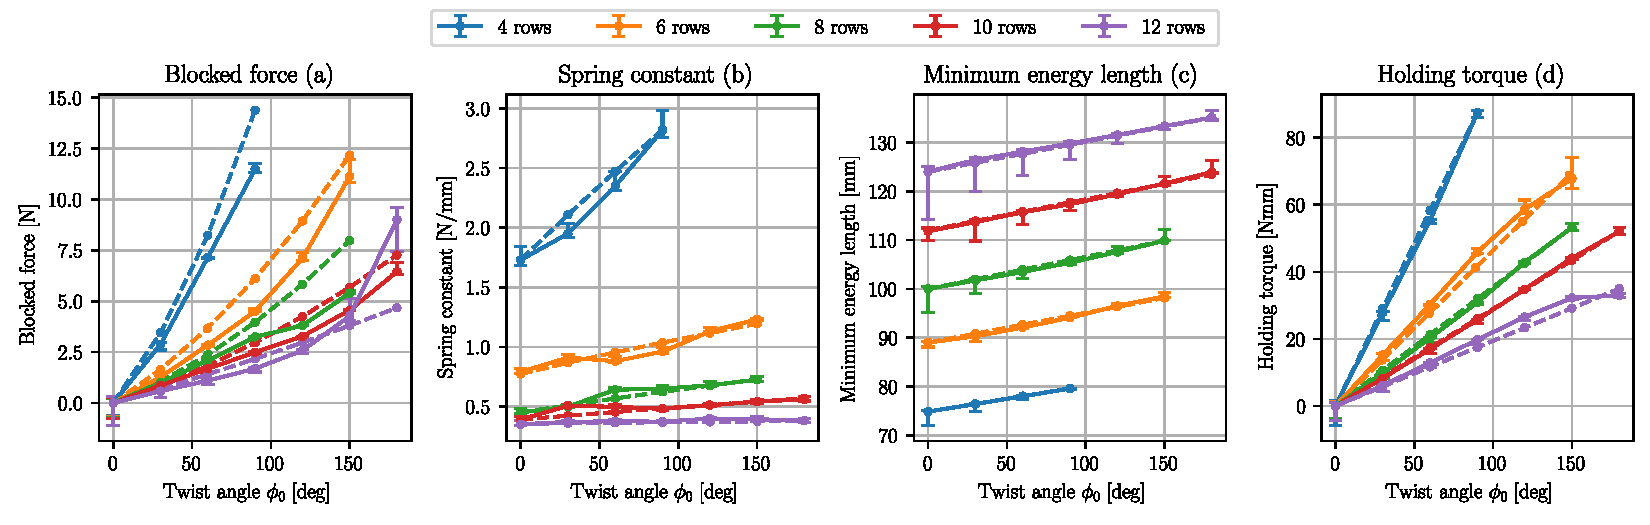
\includegraphics[width=\textwidth]{hsamodel/figures/simulation/closed_hsa_rods_verification_v2.pdf}
    \caption{Results for verification of steady-state behaviour of the proposed simulator: the solid lines represent the mechanical characteristics obtained for closed \gls{HSA} rods by Good et al.~\cite{good2022expanding} with corresponding error bars. The dashed lines correspond to the same characteristics obtained with our simulator. The simulation parameters are separately tuned for HSAs with variety of row tilings. When an HSA contains a higher number of row tiling, it will allow for larger elongations while simultaneously trading-off the spring constant~\cite{good2022expanding}.}
    \label{fig:hsamodel:closed_hsa_properties_good_et_al}
\end{figure*}

Next, we will go into more detail about each mechanical characteristic.
\textbf{Holding torque:} We apply a given torsional torque $\tau_\mathrm{h}$ at the proximal end of the \gls{HSA} and then record the twist angle of the base $\phi_0$ at steady-state.
\textbf{Minimum energy length:} The proximal end of the \gls{HSA} is rotated to a given twist angle $\phi_0$. The minimum energy length is then is identified as the steady-state length of the \gls{HSA}.
\textbf{Spring constant:} For a given twist angle $\phi_0$ with the \gls{HSA} at rest, the spring constant is identified by applying a small pulling force to the distal end and then measuring the displacement of the tip at steady-state.
\textbf{Blocked force:} Differently from the other simulations, the distal end is constrained at its initial position such as to prevent the rod from extending. The blocked force $F_\mathrm{b}$ is identified by evaluating the internal axial force for a given twist angle.
% We refer the interested reader to the paper by Good et al.~\cite{good2022expanding} for more details on the exact identification procedure of each characteristics.

% Next, we will go into more detail about the identification procedure for each property.
% \subsubsection{Holding torque}
% A given torsional torque $\tau_\mathrm{h}$ is applied to the proximal end of the \gls{HSA} rod while the dynamic behaviour of the rod is simulated for \SI{10}{s} and the last twist angle $\phi_0$ at the proximal end is recorded. This procedure is repeated for a range of torsional torques and the twist angles are plotted against their corresponding holding torques in Fig.~\ref{fig:hsamodel:closed_hsa_properties_good_et_al}(a).

% \subsubsection{Minimum energy length}
% The boundary condition at the proximal end is used to apply a given twist angle. The system is simulated for \SI{10}{s}. The final length of the rod is plotted against the twist angle in Fig.~\ref{fig:hsamodel:closed_hsa_properties_good_et_al}(b).

% \subsubsection{Spring constant}
% Again, a given twist angle is applied to the proximal end and the system is given \SI{10}{s} to converge to steady-state at the respective minimum energy length. Then, we apply a small force $F_z$ of magnitude \SI{1}{N} in z-direction to the tip of the rod and wait another \SI{10}{s} for the rod to be elongated. Subsequently, the displacement of the tip $\delta z$ with respect to the minimum energy length is computed and the spring constant is computed as $k = \frac{F_z}{\delta z}$.

% \subsubsection{Blocked force}
% Differently from the other simulations, the z-position of the distal end is constrained to remain fixed, which prevents the rod from extending. Now, a twist angle is applied at the base and the internal axial force at the tip is plotted against the twist angle.

The results show that the proposed simulator can accurately represent the steady-state behaviour of the \glspl{HSA} with the simulated characteristics mostly staying within the stated error-range of the experimental measurements by Good et al.~\cite{good2022expanding}. The only exception is Fig.~\ref{fig:hsamodel:closed_hsa_properties_good_et_al}(a), in which the simulation is overestimating the blocked force $F_\mathrm{b}$. This points to the fact that this linear approximation of the auxetic trajectory is only accurate in a limited range of the motion range of the closed \glspl{HSA}. Further research is necessary to come up with auxetic trajectory models for semi-closed and open \glspl{HSA}.

\subsection{Simulating HSA robots: boundary conditions and joints}\label{sub:hsamodel:hsa_robot_simulation:hsa_robots}
%In the previous subsections, we have devised a strategy for simulating \gls{HSA} rods and have successfully verified the steady-state behaviour of such single \glspl{HSA}. Now, 
%
We discuss here how to combine a platform and multiple \glspl{HSA} to form a \gls{HSA} robot.  Assume to have $n_\mathrm{HSA}$ rods equilly distributed along a circle of radius $R_\mathrm{cHSA}$ in the x-y plane with the rods pointing towards the positive z-direction in a straight configuration.
%
We need boundary conditions for the proximal ends of the rods to generate the parallel structure. The positions of the proximal nodes are constrained to remain at their initial position $\bar{r}_{0}$.
% $\bar{r}_{0} = \begin{pmatrix} \cos(\varphi) R_\mathrm{cHSA} & \sin(\varphi)R_\mathrm{cHSA} & 0 \end{pmatrix}^\mathrm{T}$, where $\varphi$ is the azimuth angle. 
For the same purpose, the translational rates, e.g. $v_0$, are set to zero at each time-step. 

In our plug-in to Elastica, we provide the user with two options for actuating the \glspl{HSA}. (a) The orientation of the proximal link $Q_{0}$ is moved to a desired orientation $Q_{0}^\mathrm{d}$. In this case, the twist angle $\phi_0^\mathrm{d}$ of the proximal end is controlled. Again, the rotational rates $\omega_0$ are set to zero. 
(b) Twist torques $\tau_{0,z}$ are applied to the proximal link of the \gls{HSA}. The two remaining rotational DoF (rolling and pitching) of the proximal link are constrained by setting their rotational rates $\omega_{0,x}$ and $\omega_{0,y}$ to zero.

Additionally, rigid joints between the rods and the platform are necessary. These are achieved by simulating a spring-damper system between the distal end of each \gls{HSA} and the platform. For the translations, we compute the contact force $F_\mathrm{c}$ as 
\begin{equation}
    F_\mathrm{c} = k_F \, (r_\mathrm{p}^j - r_{n_\mathrm{v}+1}) + \nu_F \, (v_\mathrm{p}^j - v_{n_\mathrm{v}+1}),
\end{equation}
where $k_F$ is the translational joint stiffness, and $\nu_F$ the translational damping coefficient. While $r_{n_\mathrm{v}+1}$, and $v_{n_\mathrm{v}+1}$ are the position and the velocity of the distal node of the rod respectively, $r_\mathrm{p}^j$ and $v_{n_\mathrm{v}+1}^j)$ are the position and velocity of the attachment point of the same rod (e.g. the $j$th rod) on the platform. We determine the position and velocity of this attachment point using rigid body kinematics with regard to the \gls{COM} of the platform. The contact force $F_\mathrm{c}$ is applied with an opposite sign to the distal end of the \gls{HSA} and to the platform, respectively. Please note that the contact force $F$ also generates a torque $\tau_{F_\mathrm{c}}$ on the platform, as the force is not applied at the \gls{COM} of the rigid body.

Similarly to the contact force, a contact torque $\tau_\mathrm{c}$ is computed to reduce any error in the orientation and angular velocity between the two systems
\begin{equation}
    \tau_\mathrm{c} = k_\tau \, (Q_\mathrm{p}^\mathrm{T} \log(Q_\mathrm{p} \, Q_{n_\mathrm{v}}^\mathrm{T})) + \nu_\tau \, (Q_\mathrm{p}^\mathrm{T} \omega_\mathrm{p}^j - Q_{n_\mathrm{v}}^\mathrm{T} \omega_{n_\mathrm{v}})
\end{equation}
where the $\log(\cdot): \mathbb{R}^{3 \times 3} \rightarrow $ operator computes the rotation vector from the rotation matrix~\cite{gazzola2018forward}, and $Q_\mathrm{p}$ is the material frame of the platform.

\subsection{Qualitative evaluation of motion primitives in simulation}\label{sub:hsamodel:hsa_robot_simulation:motion_primitives}
We reproduce the typical motion primitives of a \gls{HSA} robot consisting of four \glspl{HSA} (e.g. $n_\mathrm{HSA} = 4$) in simulation and show the final steady-states in Fig.~\ref{fig:hsamodel:motion_primitives}. Two of the \glspl{HSA} are left-handed and positioned diagonally from each other. 
Each rod is discretized by $n_\mathrm{v} = 25$ links and $26$ point mass vertices. Furthermore, it has a printed length of $\Bar{L} = \SI{100}{mm}$, an outside radius of \SI{25.4}{mm} and a wall-thickness of \SI{2.43}{mm}. The rods are placed at a radial distance of $R_\mathrm{cHSA} = \SI{24}{mm}$ from the center of the robot and a material density of $\rho_\mathrm{HSA} = \SI{1050}{kg \per m^3}$ is assumed. Therefore, the chosen simulation parameters mirror the geometric characteristics of our experimental platform.
Based on an elastic modulus $E=\SI{10}{MPa}$ and a shear modulus $G=\SI{0.6}{MPa}$, the shear and stretch stiffnesses amount to $S_{x,y} = \SI{101.5}{N \per m}$, and $S_z = \SI{1753.5}{N \per m}$.
We set the bend and twist rigidities $B_{x}, B_y$, and $B_z$ to \SI{0.02}{Nm^2 \per rad} and \SI{0.014}{Nm^2 \per rad} respectively. When twist strains are present, we extend the rest length of the rod by \SI{0.01}{m \per rad} after taking into account the handedness of the \gls{HSA}.

The cylindrical platform is of diameter \SI{95}{mm}, has a thickness of \SI{3}{mm} and is modelled to have a density of $\rho_\mathrm{p} = \SI{700}{kg / m^3}$.
The joint stiffness parameters $k_F = 5\cdot 10^5 \: \si{N \per m}$ and $k_\tau = 20 \: \si{Nm \per rad}$ are chosen for the fixed joint between \glspl{HSA} and platform. The joint damping coefficients $\nu_F$, $\nu_\tau$ are set to zero.

Our qualitative results in Fig.~\ref{fig:hsamodel:motion_primitives} demonstrate that we are able to generate all motion primitives in simulation. For the shown deformations, we apply maximum twist angles of $\phi_{0,\mathrm{max}} = \pi \, \si{rad}$. % It needs to be noted that the axial stiffness $S_x$ (e.g. $E$-modulus), the bend rigidites $B_x, B_y$, the twist stiffness $B_z$, and the shear rigidities $S_y, S_z$ need to be carefully tuned to produced the desired \gls{HSA} deformations, particularly during the twisting motion primitive.
\section{A Kinematic Model for HSA Rods}\label{sec:hsamodel:hsa_rod_kinematics}
In this section, we aim to derive a forward kinematic model that can be used to describe the shape of a single \gls{HSA} rod with a minimum amount of parameters. More specifically, we want to describe the transformation from the base frame $\{ S_{\mathcal{B}} \}$ to a local frame $\{ S_s \}(q,s)$ at a coordinate $s \in [0, \Bar{L}]$. This coordinate lies on the backbone of an \gls{HSA} rod of printed (i.e. initial) length $\Bar{L}$.

\subsection{Selective Piecewise Constant Strain (SPCS) kinematics}\label{sub:hsamodel:hsa_rod_kinematics:spcs_kinematics}
For this purpose, we combine the existing kinematic models \gls{CS} and \gls{PCS}~\cite{renda2018discrete} to selectively keep specific strains constant along the entire length of the robot or vary them piece-wise among the segments.
%Opposite to existing kinematic models based on \gls{CC}~\cite{garg2022kinematic}, our kinematic description strives to model the twist of the \gls{HSA} rod.
This parametrization can be combined with the results in Sec.~\ref{sec:hsamodel:hsa_robot_simulation} to generate a compact dynamic model for the movement of HSA robots in 3D space.
\begin{figure}[htb]
    \centering
    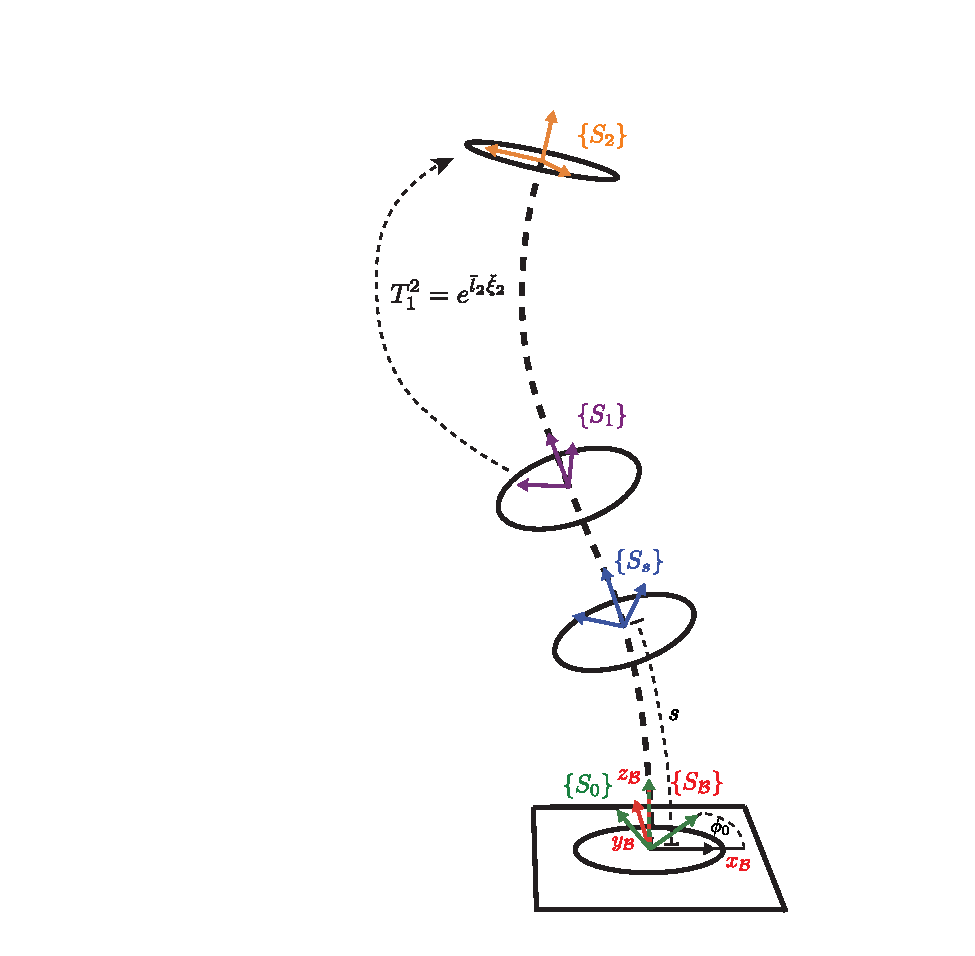
\includegraphics[width=0.25\columnwidth]{hsamodel/figures/kinematics/twisting_kinematics_v2_cropped.pdf}
    \caption{Visualization of the proposed \gls{SPCS} kinematic model for the case of $n_\mathrm{S} = 2$ segments: The forward kinematics describe a transformation from the base frame $\{ S_{\mathcal{B}} \}$ to the local frame $\{ S_s \}$ at the coordinate $s \in [0, \bar{L}]$ and consist of a) a rotation around the $z_{\mathcal{B}}$-axis of the base frame by angle $\phi_0$, b) an exponential map $e^{(s-\bar{L}_i) \, \check{\xi}_i}$ for the transformation from the proximal end of the $i$th segment to the local frame of the coordinate $s$. % The strain $\xi_i$ consists of a rest strain $\hat{xi}$, a strain $\xi_{\mathrm{CS}}$ constant along the entire rod, and finally a strain component specific to the $i$th segment $\xi_{\mathrm{PCS},i}$.
    }
    \label{fig:hsamodel:hsa_kinematics}
\end{figure}

First, we define that 
\begin{equation}
    \xi(q,s) = \begin{pmatrix} \kappa_x & \kappa_y & \kappa_z & \sigma_x & \sigma_y & \sigma_z \end{pmatrix}^\mathrm{T} \in \mathbb{R}^6
\end{equation}
represents the three rotational and three linear strains present in a rod~\cite{renda2018discrete}. Subsequently, propose the following configuration vector for an \gls{HSA}
\begin{equation}
    q = \begin{pmatrix}
        \phi_0 & q_\mathrm{CS}^\mathrm{T} & q_{\mathrm{PCS},1}^\mathrm{T} & \cdots & q_{\mathrm{PCS},i}^\mathrm{T} & \cdots & q_{\mathrm{PCS},n_\mathrm{S}}^\mathrm{T}
    \end{pmatrix}^\mathrm{T}% \in \mathbb{R}^{1 + n_{q,\mathrm{CS}} + n_\mathrm{S} \: n_{q,\mathrm{PCS}}},
\end{equation}
where $\phi_0 \in \mathbb{R}$ is the twist angle at the base and allows for the rotation of the motor actuating the \gls{HSA} rod. $q_\mathrm{CS} \in \mathbb{R}^{n_{q,\mathrm{CS}}}$ is a strain component constant along the entire rod, and $q_{\mathrm{PCS},i} \in \mathbb{R}^{n_{q,\mathrm{PCS}}}, i \in \{1, \dots, n_\mathrm{PCS}\}$ is the configuration of each \gls{PCS} segment. The $i$th segment has a initial length of $\bar{l}_i$ with its tip at the coordinate $\bar{L}_i$
%
The strain in the $i$th segment is then the sum of the rest strain $\hat{\xi} = \begin{pmatrix} 0 & 0 & 0 & 0 & 0 & 1\end{pmatrix}^\mathrm{T}$, $\xi_\mathrm{CS}$, and $\xi_{\mathrm{PCS},i}$:
\begin{equation}
    \xi_i = \hat{\xi} + B_\mathrm{CS} \: q_\mathrm{CS} + B_{\mathrm{PCS},i} \: q_{\mathrm{PCS},i}, \quad i \in \{1,\dots, n_\mathrm{S}\}.
\end{equation}
Analogue to the concept introduced in \cite{renda2020geometric}, $B_\mathrm{CS} \in \mathbb{R}^{6 \times n_{q,\mathrm{CS}}}$, $B_\mathrm{PCS} \in \mathbb{R}^{6 \times n_{q,\mathrm{PCS}}}$ are the strain bases of $q_\mathrm{CS}$ and $q_\mathrm{PCS}$ respectively.

In this chapter, we specifically investigate a setting where the twist \& stretch strains are constant across the entire rod and the bend \& shear strains vary for each segment.
Accordingly, we choose $q_\mathrm{CS} = \begin{pmatrix} \kappa_z & \sigma_z \end{pmatrix}^\mathrm{T}$ and $q_{\mathrm{PCS},i} = \begin{pmatrix} \kappa_{x,i} & \kappa_{y,i} & \sigma_{x,i} & \sigma_{y,i} \end{pmatrix}^\mathrm{T}$.
Then, the corresponding strain bases are determined to be
\begin{equation}
\begin{split}
    B_\mathrm{CS} = \begin{bmatrix}
        0 & 0 & 1 & 0 & 0 & 0\\
        0 & 0 & 0 & 0 & 0 & 1\\
    \end{bmatrix}^\mathrm{T} \in \mathbb{R}^{6 \times 2},\\
    B_{\mathrm{PCS},i} = \begin{bmatrix}
        1 & 0 & 0 & 0 & 0 & 0\\
        0 & 1 & 0 & 0 & 0 & 0\\
        0 & 0 & 0 & 1 & 0 & 0\\
        0 & 0 & 0 & 0 & 1 & 0\\
    \end{bmatrix}^\mathrm{T} \in \mathbb{R}^{6 \times 4}.
\end{split}
\end{equation}

Next, we find homogeneous forward kinematic mappings for the given configuration and strains.
As the twist angle $\phi_0$ demands a rotation around the local $z_{\mathcal{B}}$-axis of the base frame, the matrix $R_{\mathcal{B}}^0(\phi_0) \in SO(3)$ contains the rotation from the base frame $\{ S_{\mathcal{B}} \}$ to the proximal end of the rod denoted as frame $\{ S_{0} \}$.
For a point $s$ on the $i$th segment with constant strain $\xi_i$, the transformation matrix from the segment's proximal frame $\{ S_{i-1} \}$ to the local frame at coordinate $s$ is given by the exponential map $e: \mathfrak{se}(3) \mapsto SE(3)$~\cite{renda2018discrete}
\begin{equation}
\begin{split}
    e^{(s-\bar{L}_{i-1}) \check{\xi}_i} =& I_4 + (s-\bar{L}_{i-1}) \, \check{\xi}_i + \left ( 1 - \cos((s-\bar{L}_{i-1}) \, \theta_i) \right )\\ 
    &\frac{\check{\xi}_i^2}{\theta_i^2} + \left ( (s-\bar{L}_{i-1}) \, \theta_i - \sin((s-\bar{L}_{i-1}) \theta_i) \right ) \frac{\check{\xi}_i^3}{\theta_i^3}.
\end{split}
\end{equation}
where $\check{\xi}_i \in \mathfrak{se}(3)$ is the strain twist vector and $\theta_i = \sqrt{\kappa_{x,i}^2 + \kappa_{y,i}^2 + \kappa_{z,i}^2}$ is the magnitude of the rotational strain.
Therefore, the fully assembled transformation $T_{\mathcal{B}}^i(q)$ from the base frame $\{ S_{\mathcal{B}} \}$ to the tip frame of the $i$th segment can be expressed as
\begin{equation}
    T_{\mathcal{B}}^i(q) = T_{\mathcal{B}}^0(\phi_0) \, \Pi_{j=1}^{i} \: e^{\bar{l}_{j} \check{\xi}_{j}}(q) \in SE(3).
\end{equation}

% \begingroup
% \setlength{\tabcolsep}{3pt} % Default value: 6pt
% \begin{table}
% \centering
% \caption{Verification of kinematic model in simulation.}
% \begin{tabular}{l c c ccc}\toprule
% \textbf{Dataset} & $e_t$ [mm] & $e_\mathrm{quat}$ [-] & $e_\mathrm{eul,x}$ [rad] & $e_\mathrm{eul,y}$ [rad] & $e_\mathrm{eul,z}$ [rad]\\
% \midrule
% Elongation & \SI{0.042}{mm} & $0.00027$ & $5.6\mathrm{e}{-9}$ \si{rad} & $1.9\mathrm{e}{-8}$ \si{rad} & $1.7\mathrm{e}{-6}$ \si{rad}\\
% \bottomrule
% \end{tabular}
% \label{tab:hsamodel:kinematic_results_simulation}
% \end{table}
% \endgroup

\begin{figure}[t]
    \centering
    \subfigure{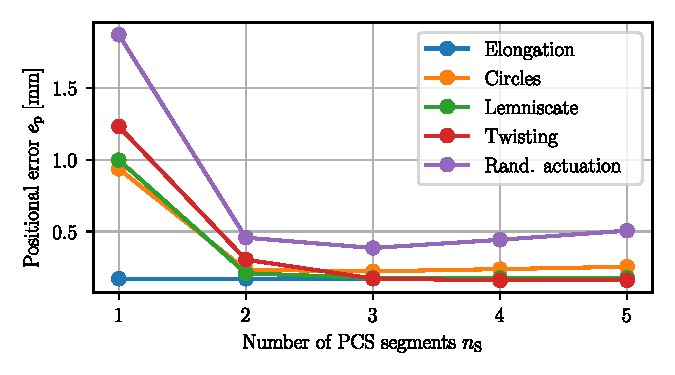
\includegraphics[width=0.49\columnwidth]{hsamodel/figures/simulation_plots/Kinematic_position_error_vs._number_of_PCS_segments_v3_cropped.pdf}}
    \subfigure{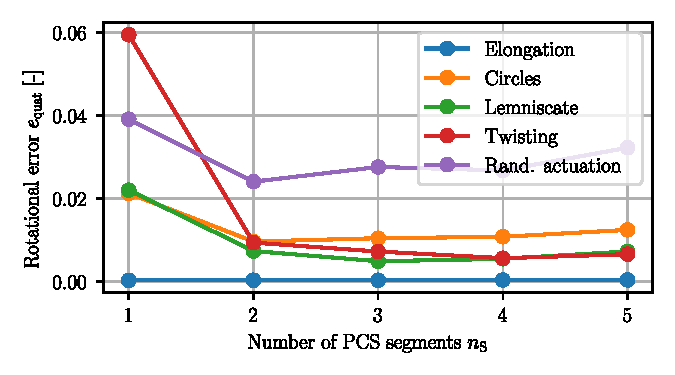
\includegraphics[width=0.49\columnwidth]{hsamodel/figures/simulation_plots/Kinematic_rotation_error_vs._number_of_PCS_segments_v3_cropped.pdf}}
    
    \caption{Verification of kinematic models in simulation. 
    The plot in the first row shows the positional error $e_\mathrm{p}$ of the kinematic model against the simulated HSA. The plot in the second row visualizes the rotational error metric $e_\mathrm{quat}$, which is based on the vector component of the unit quaternion. For more information on the evaluation metrics, we refer to Section~\ref{ssub:hsamodel:hsa_rod_kinematics:evaluation_metrics}.
    %The poses of $25$ points along the rod determined through forward kinematics of a regressed configuration are compared against the links of a simulated, discretized Cosserat rod. 
    The kinematic model used here assumes the twist \& stretch strains to be constant along the entire HSA and the bend \& shear strains to be captured by $n_\mathrm{S}$ segments.
    Along this line, we report the performance of the kinematic model for a parametrization containing one to five segments.
    }\label{fig:hsamodel:hsa_robot_simulation_kinematic_error_vs_number_of_PCS_segments}
\end{figure}

% \subsection{Differential Kinematics}
% Derive Jacobian etc.

% \begin{SCfigure*}
%     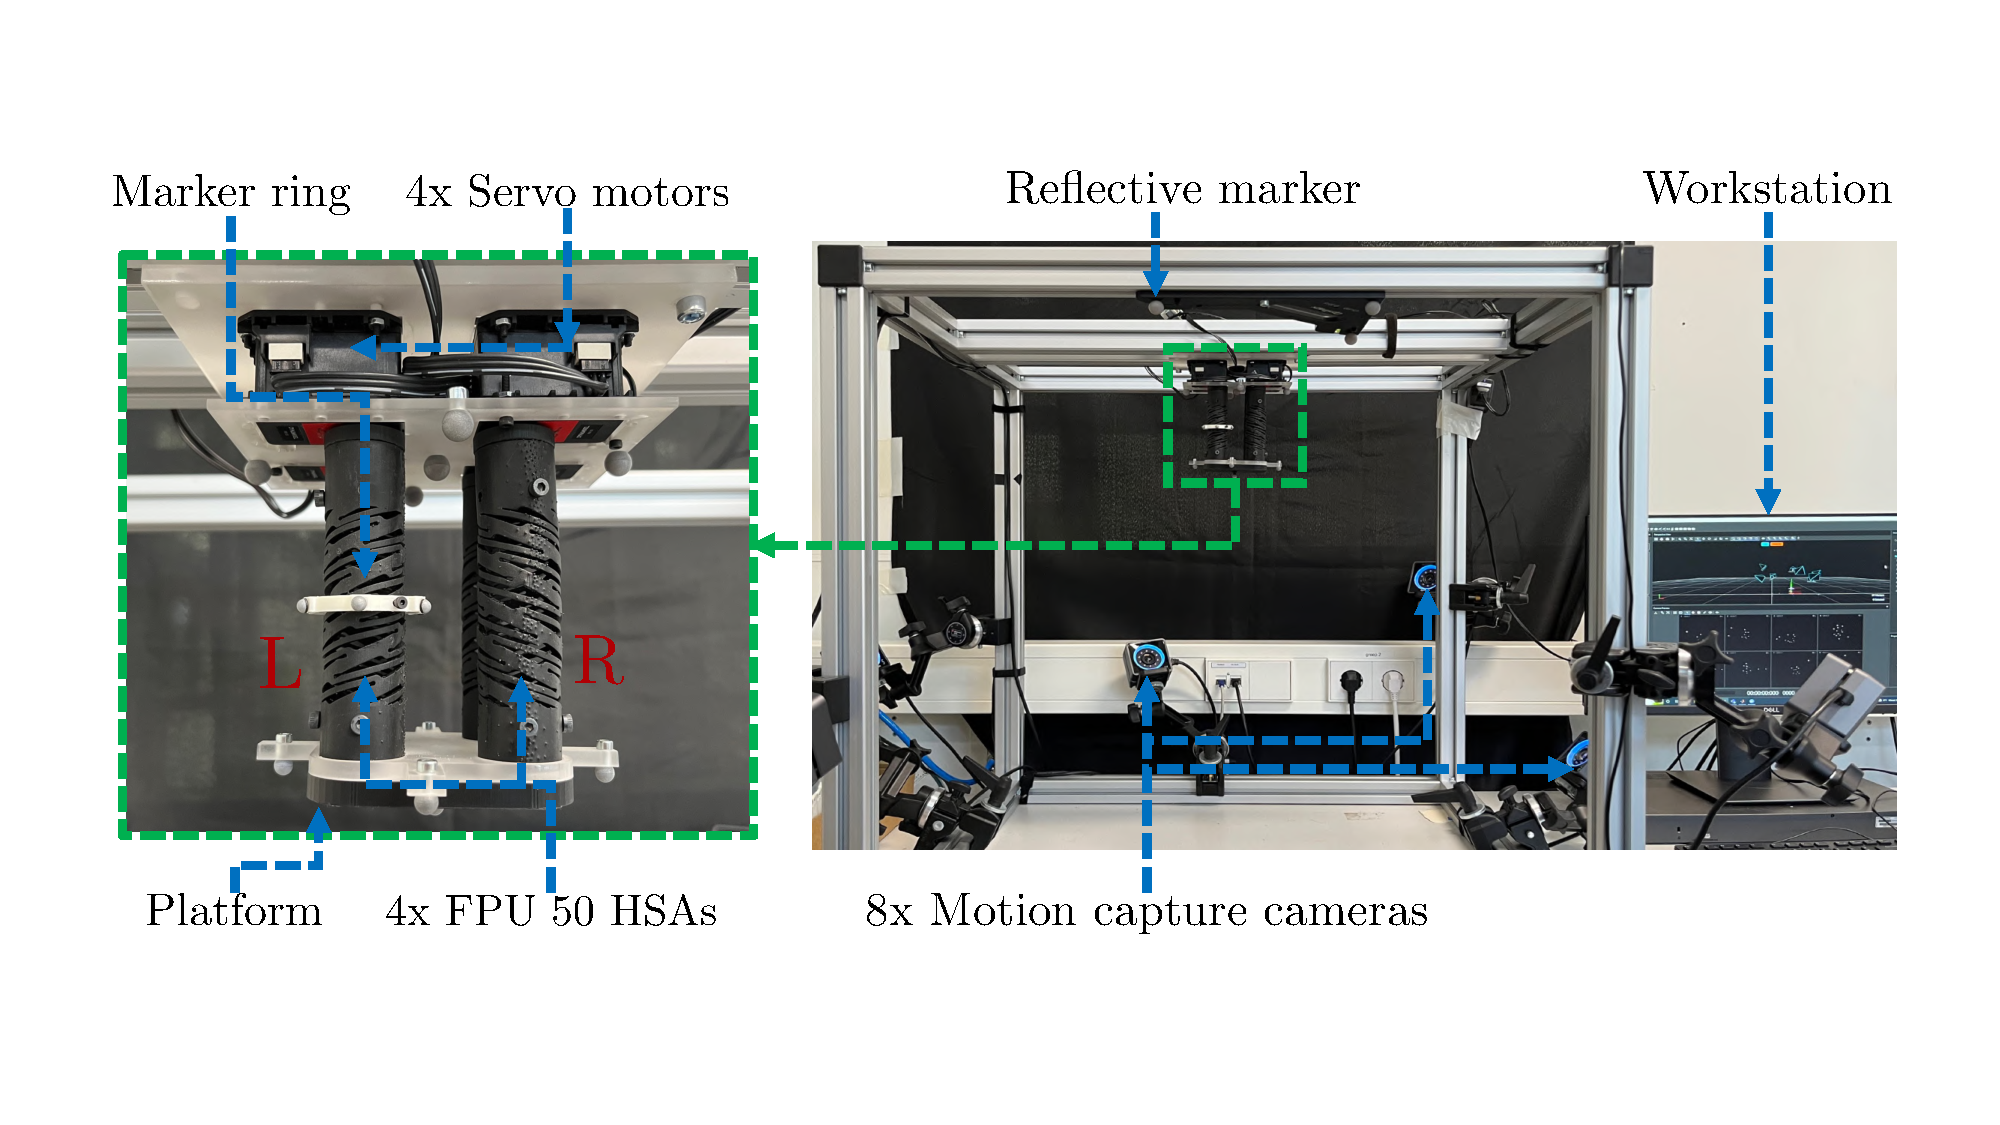
\includegraphics[width=0.75\textwidth]{hsamodel/figures/experimental_setup/experimental_setup_v3_compressed.pdf}
%     \caption{Experimental setup with the \gls{HSA} robot attached in platform-down configuration to the motion capture cage. The robot contains two left-handed (L) and two right-handed (R) \gls{HSA} rods respectively. Rods of the same handedness are placed opposite of each other. The reflective markers allow us to determine the pose information of the base, an intermediate point along the left \gls{HSA} rod, and the platform.}\label{fig:hsamodel:experimental_setup}
% \end{SCfigure*}

\begin{figure*}
    \centering
    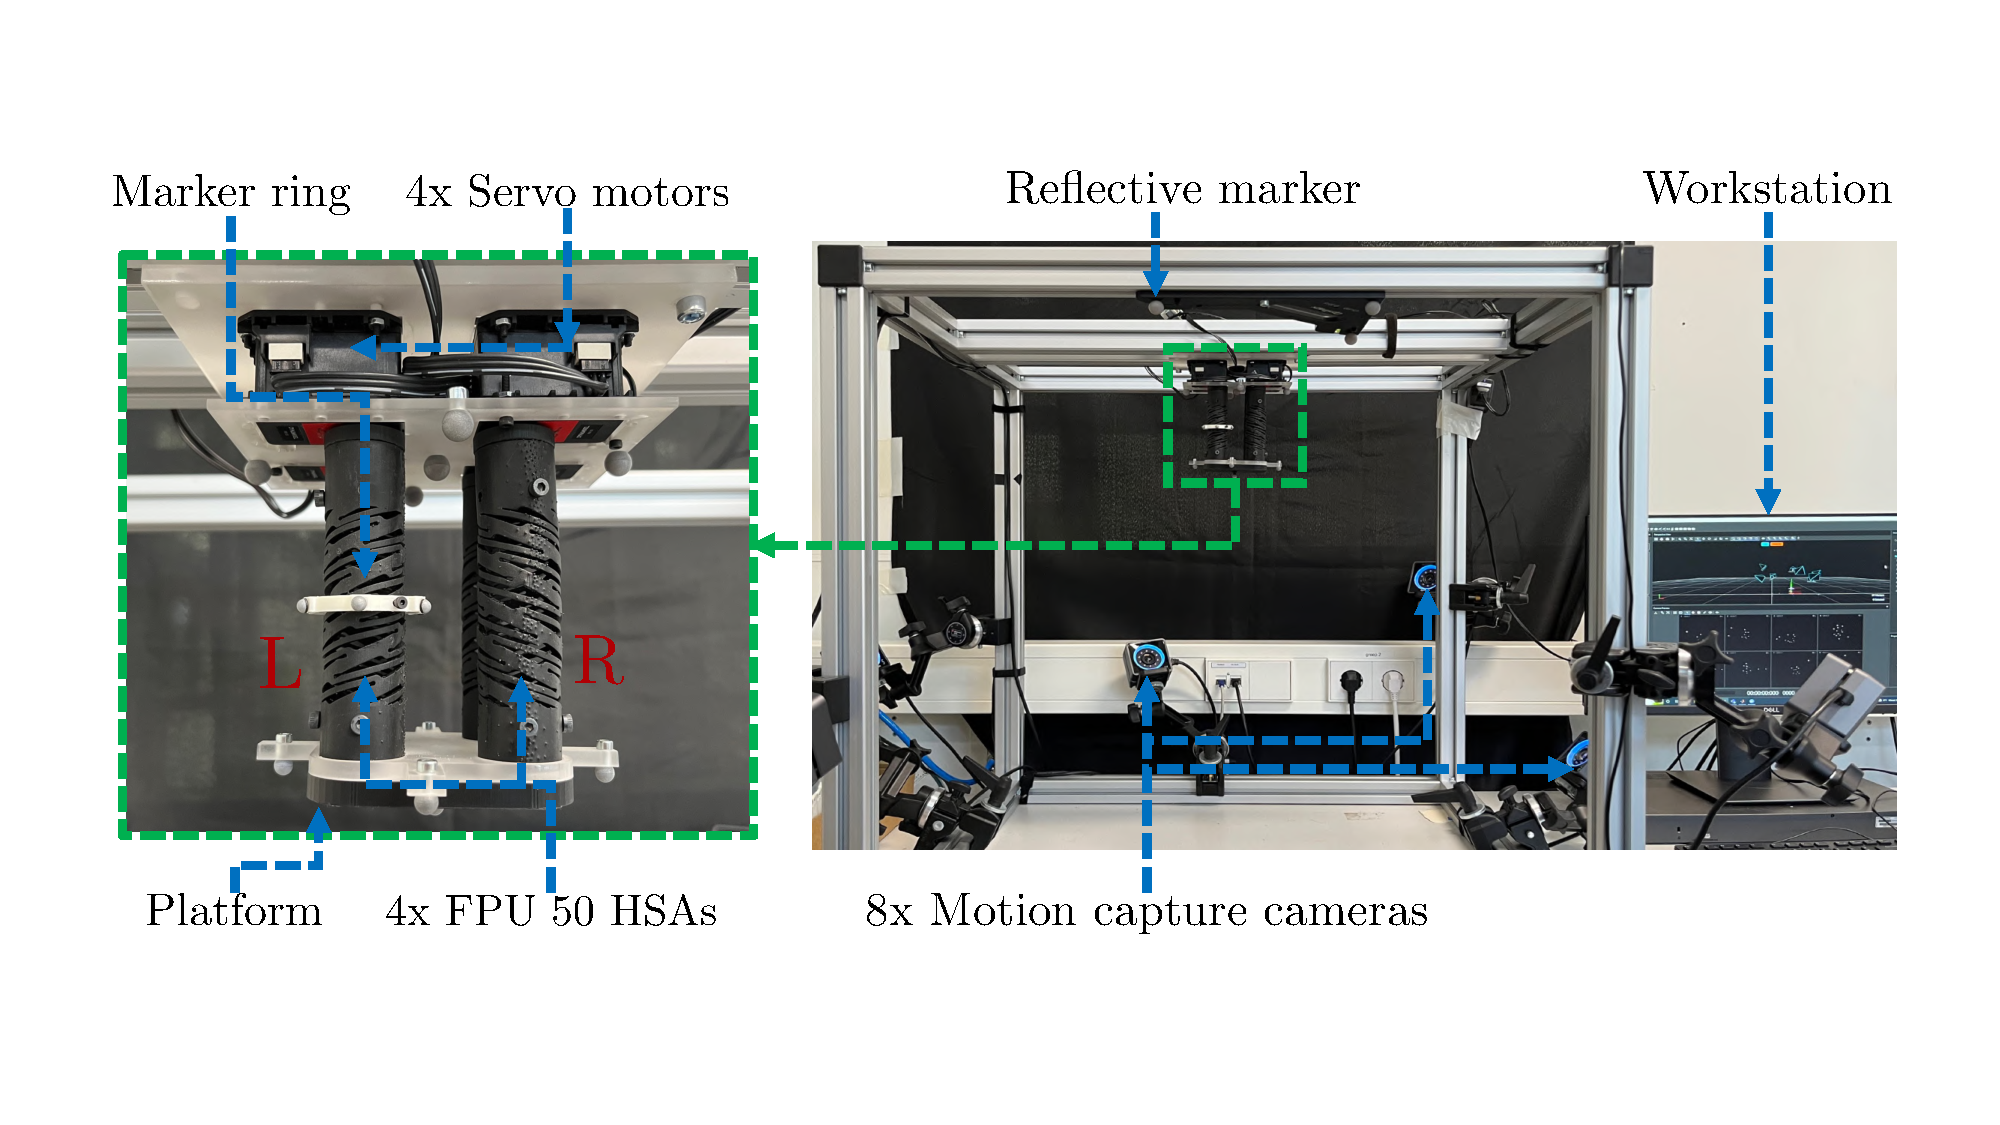
\includegraphics[width=0.77\textwidth]{hsamodel/figures/experimental_setup/experimental_setup_v3_compressed.pdf}
    \caption{Experimental setup with the \gls{HSA} robot attached in platform-down configuration to the motion capture cage. The robot contains two left-handed (L) and two right-handed (R) \gls{HSA} rods, respectively. Rods of the same handedness are placed opposite of each other. The reflective markers allow us to determine the pose information of the base, an intermediate point along the left \gls{HSA} rod, and the platform.}\label{fig:hsamodel:experimental_setup}
\end{figure*}



\subsection{Verification of the SPCS kinematics}\label{sub:hsamodel:hsa_rod_kinematics:verification}
The section is structured as follows. We introduce relevant actuation sequences for the \gls{HSA} robot.
Next, we present an inverse kinematic approach to identify the kinematic configuration.
Translational and rotational error metrics are then defined to evaluate the quality of reconstructions. %mismatch between the poses predicted by the kinematic model and the actual measurements.
% Finally, we investigate the importance of the various strains and the performance with respect to the number of \gls{CS} segments for both simulation data and experimental datasets.
Finally, we verify the performance of the proposed \gls{SPCS} kinematic model both for simulated data and on experimental datasets.
The code and all datasets are made available on GitHub~\footnote{\scriptsize \url{https://github.com/tud-phi/hsa-kinematic-model}}.

\subsubsection{Actuation sequences}\label{ssub:hsamodel:hsa_rod_kinematics:actuation_sequences}
We collect datasets with a variety of actuation sequences, which include both pure motion primitives and random actuation. 
% The elongation, bending, and twisting motion primitives are invoked with the specifications in Fig.~\ref{fig:hsamodel:motion_primitives}(a). 
For all sequences, we apply a twist angle of magnitude  $|u_\mathrm{d}| \in [0, \pi \: \si{rad}]$ at the base of each \gls{HSA}. The sign of $u_\mathrm{d}$ is determined by the handedness $h$ of the respective \gls{HSA}.
The elongation dataset consists of samples between the rest and fully-elongated \gls{HSA} state. Please refer to Fig.~\ref{fig:hsamodel:motion_primitives}(a) for more details on how each motion primitive can be invoked.
For the bending motion primitive, we consider two separate trajectory types: a) a Lemniscate trajectory and b) a trajectory containing circles of varying bending angles. The different bending angles are achieved by varying the actuation angle from $\SI{20}{\percent}$ to \SI{100}{\percent} of its maximum magnitude. For each fixed bending angle, we collect $15$ samples along the circle, e.g. $15$ different azimuth angles.
To achieve the desired azimuth angle, we smoothly interpolate between the east, north, west, and south actuation specifications of Fig.~\ref{fig:hsamodel:motion_primitives}(a).
The twisting trajectory collects discrete samples between maximum clockwise (CW) and maximum counter-clockwise (CCW) twisting.
Finally, we collect a dataset of randomly sampled actuation inputs, which combines the elongation, bending, and twisting motion primitives. % More specifically, we randomly the azimuth angle of bending from a uniform distribution $\mathcal{U}(0,2\pi)$.
In total, the elongation and Lemniscate trajectories contain $100$ samples each, and the circles and twisting trajectory have $225$ and $100$ samples, respectively. $500$ samples are included in the random actuation actuation sequence.


% We consider different datasets as part of this study. In some datasets, we actuate the \gls{HSA} robot such as to exhibit one of the motion primitives purely (e.g. elongation, bending, and twisting). Contrarily, the \emph{random actuation} dataset combines these motion primitives as we randomly sample each motor position $u_j \in h_j \, \mathcal{U}(0,\pi \, \si{rad})$. 

\subsubsection{Inverse kinematics}\label{ssub:hsamodel:hsa_rod_kinematics:inverse_kinematics}
Differential inverse kinematics can be used to reconstruct the rod's configuration $q$ from $N$ known poses $T_{\mathcal{B}}^{s_i} \in SE(3), i \in [1, N]$ along the rod. 
%While any of the standard Jacobian-based inverse differential kinematics approaches from literature~\cite{siciliano2009differential} could be used, 
We implemented an inverse kinematics algorithm based on the analytical Jacobian $J_\mathrm{A}^{s_i} \in \mathbb{R}^{6 \times 7}$ of the pose representation
\begin{equation*}
    \chi_{\mathcal{B}}^{s_i} = \begin{pmatrix}
        \varepsilon_x & \varepsilon_y & \varepsilon_z & \eta & \varepsilon_z & p_x & p_y & p_z
    \end{pmatrix}^\mathrm{T} \in \mathbb{R}^{7},
\end{equation*}
which includes rotational orientation estimates in unit quaternion representation $\mathcal{Q} = \begin{pmatrix} \varepsilon_x & \varepsilon_y & \varepsilon_z & \eta \end{pmatrix}^\mathrm{T}$ and positions in Cartesian space $p = \begin{pmatrix} p_x & p_y & p_z \end{pmatrix}^\mathrm{T}$.
Please note that usually $\phi_0$ does not need to be found through (differential) inverse kinematics but can rather be directly read out from the encoders of the electric servos.
All $N$ poses and Jacobians can be vertically stacked as $\chi \in \mathbb{R}^{7N}$  and $J_\mathrm{A} \in \mathbb{R}^{7N \times 6}$  respectively. This then allows us to then iteratively optimize the pose error $e_\chi = \chi_\mathrm{d} - \tilde{\chi}$ between the known pose $\chi_\mathrm{d}$ and the pose $\tilde{\chi}$ computed using the forward kinematics
\begin{equation}
    \tilde{q}_{\mathrm{it} + 1} = \tilde{q}_{\mathrm{it}} + \lambda \, J_\mathrm{A}^\mathrm{T}(\tilde{q}) \, \left ( \chi_\mathrm{d} - \tilde{\chi}(\tilde{q}) \right ),
\end{equation}
where $\tilde{q}$ is the current configuration estimate, and $\lambda$ is the step size.

\begingroup
\setlength{\tabcolsep}{2pt} % Default value: 6pt
\begin{table}\scriptsize
\centering
\caption{Experimental verification of kinematic models on an HSA robot. Motion capture markers attached to one of the \glspl{HSA} provide two ground-truth poses along the rod,
and we measure $\phi_0$ from the servo readings ($13$ constraints in total). %Therefore, we have in total $13$ constrains for the kinematic model.
% We evaluate on a variety of datasets collected with actuation sequences mirroring certain motion primitives such as pure elongation, pure bending, and pure twisting. Additionally, we also consider a dataset with random actuation angles. As a consequence, this dataset contains samples exhibiting all three motion primitives simultaneously. 
In the spirit of an ablation study, we investigate different variations of the proposed kinematic parametrization.
For Constant Curvature (CC), Constant Twist (CT), Constant Shear (CSH), and Constant Axial (CA) strain, the strain is kept constant along the entire HSA.
For Piecewise Constant Curvature (PCC), Piecewise Constant Twist (PCT), Piecewise Constant Shear (PCSH), and Piecewise Constant Axial (PCA) strain, the strain components are parameterized separately for each of the two segments.
% All kinematic parametrization use two Piecewise Constant Strain (PCS) segments.
Additionally, we test the importance of including the shear strain component.
For each kinematic parametrization, we state the Degrees of Freedom (DoF). 
We report RMSEs for both translations and rotations (see Sec.~\ref{ssub:hsamodel:hsa_rod_kinematics:evaluation_metrics}).}
\begin{tabular}{l cccc cccc c c c ccc}\toprule
\textbf{Trajectory} & \textbf{CC} & \textbf{CT} & \textbf{CSH} & \textbf{CA} & \textbf{PCC} & \textbf{PCT} & \textbf{PCSH} & \textbf{PCA} & \textbf{DoF} & $e_\mathrm{p}$ [mm] & $e_\mathrm{quat}$ [-] & $e_\mathrm{eul,\alpha}$ [rad] & $e_\mathrm{eul,\beta}$ [rad] & $e_\mathrm{eul,\gamma}$ [rad]\\
\midrule
Elongation & \xmark & \cmark & \xmark & \cmark & \cmark & \xmark & \xmark & \xmark & $7$ & $1.010$ & $0.0092$ & $0.0029$ & $0.0079$ & $0.0166$\\
Elongation & \xmark & \cmark & \xmark & \cmark & \cmark & \xmark & \cmark & \xmark & $11$ & $0.126$ & $0.0082$ & $0.0020$ & $0.0031$ & $0.0166$\\
Elongation & \xmark & \xmark & \xmark & \xmark & \cmark & \cmark & \cmark & \cmark & $13$ & $0.009$ & $0.0042$ & $0.0020$ & $0.0031$ & $0.0070$\\
\midrule
Circles & \xmark & \cmark & \xmark & \cmark & \cmark & \xmark & \xmark & \xmark & $7$ & $1.744$ & $0.0136$ & $0.0108$ & $0.0123$ & $0.0228$\\
Circles & \xmark & \cmark & \xmark & \cmark & \cmark & \xmark & \cmark & \xmark & $11$ & $0.227$ & $0.0082$ & $0.0110$ & $0.0122$ & $0.0227$\\
Circles & \xmark & \xmark & \xmark & \xmark & \cmark & \cmark & \cmark & \cmark & $13$ & $0.092$ & $0.0093$ & $0.0116$ & $0.0125$ & $0.0075$\\
\midrule
Lemniscate & \xmark & \cmark & \xmark & \cmark & \cmark & \xmark & \xmark & \xmark & $7$ & $1.227$ & $0.0098$ & $0.0042$ & $0.0051$ & $0.0195$\\
Lemniscate & \xmark & \cmark & \xmark & \cmark & \cmark & \xmark & \cmark & \xmark & $11$ & $0.215$ & $0.0082$ & $0.0045$ & $0.0053$ & $0.0195$\\
Lemniscate & \xmark & \xmark & \xmark & \xmark & \cmark & \cmark & \cmark & \cmark & $13$ & $0.023$ & $0.0052$ & $0.0043$ & $0.0054$ & $0.0076$\\
\midrule
Twisting & \xmark & \cmark & \xmark & \cmark & \cmark & \xmark & \xmark & \xmark & $7$ & $2.931$ & $0.0136$ & $0.0121$ & $0.0186$ & $0.0195$\\
Twisting & \xmark & \cmark & \xmark & \cmark & \cmark & \xmark & \cmark & \xmark & $11$ & $0.263$ & $0.0141$ & $0.0130$ & $0.0196$ & $0.0194$\\
Twisting & \xmark & \xmark & \xmark & \xmark & \cmark & \cmark & \cmark & \cmark & $13$ & $0.030$ & $0.0127$ & $0.0131$ & $0.0217$ & $0.0017$\\
\midrule
Rand. actuation & \xmark & \cmark & \xmark & \cmark & \cmark & \xmark & \xmark & \xmark & $7$ & $4.345$ & $0.0381$ & $0.0678$ & $0.0544$ & $0.0195$\\
Rand. actuation & \xmark & \cmark & \xmark & \cmark & \cmark & \xmark & \cmark & \xmark & $11$ & $0.365$ & $0.0383$ & $0.0681$ & $0.0544$ & $0.0193$\\
Rand. actuation & \xmark & \xmark & \xmark & \xmark & \cmark & \cmark & \cmark & \cmark & $13$ & $0.255$ & $0.0380$ & $0.0700$ & $0.0527$ & $0.0200$\\
\bottomrule
\end{tabular}
\label{tab:hsamodel:kinematic_results_experiments}
\end{table}
\endgroup

\begin{figure*}[t]
    \centering
    \subfigure[Lemniscate trajectory]{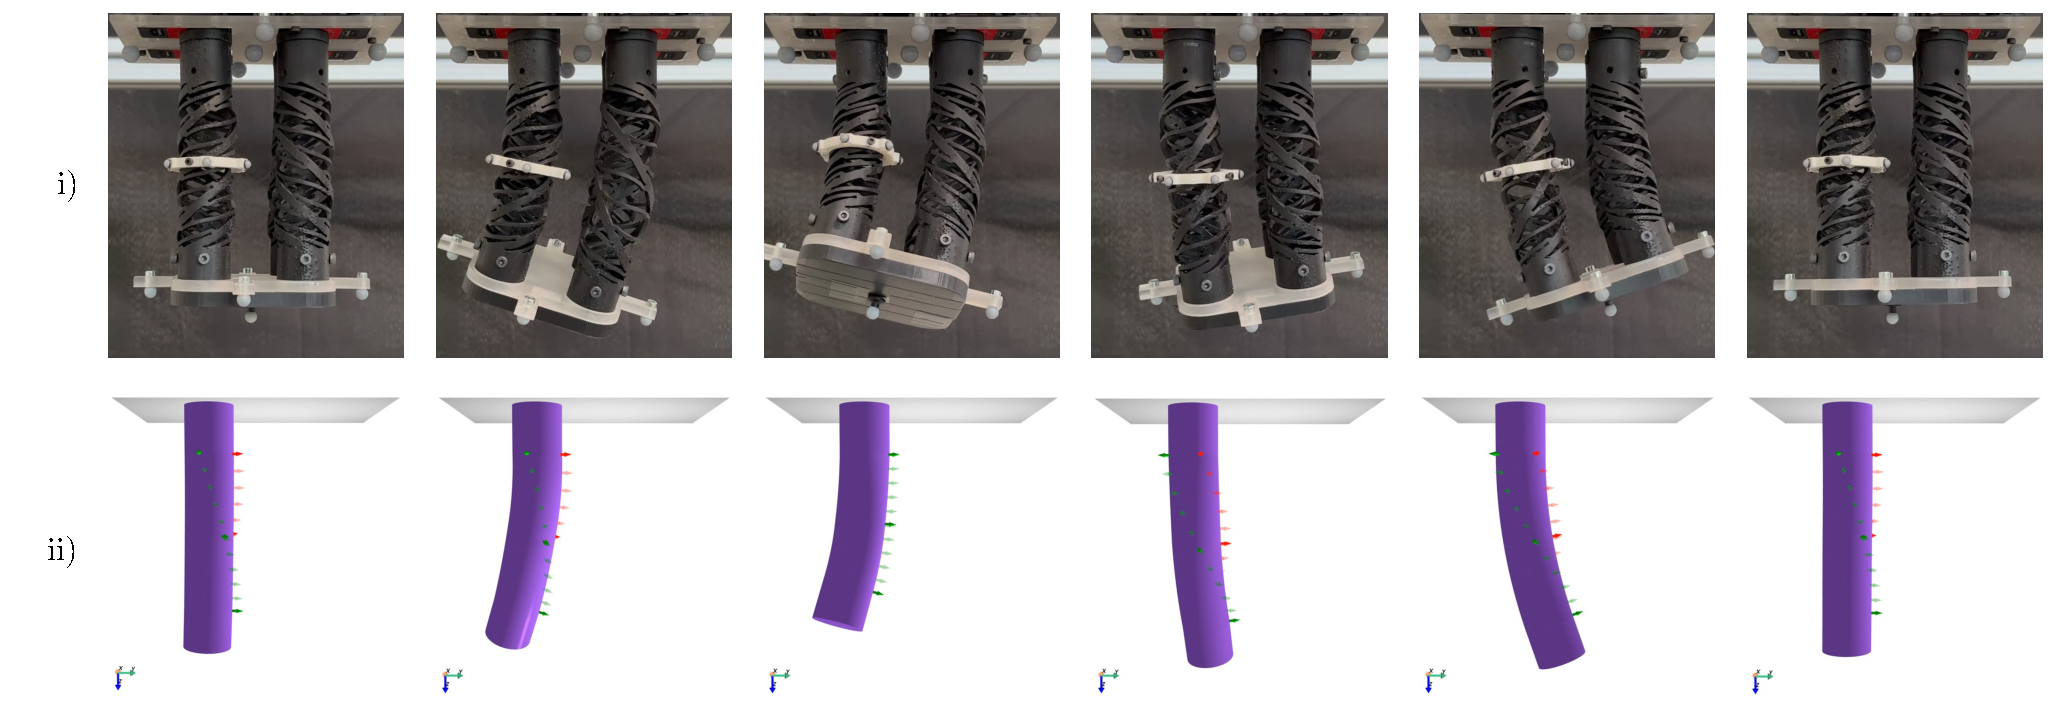
\includegraphics[width=0.95\textwidth]{hsamodel/figures/experiments_sequence_of_stills/experiment_lemniscate_inverse_kinematics_sequence_of_stills_v2_compressed.pdf}\label{fig:hsamodel:experiment_lemniscate_inverse_kinematics_sequence_of_stills}}
    \subfigure[Twisting trajectory]{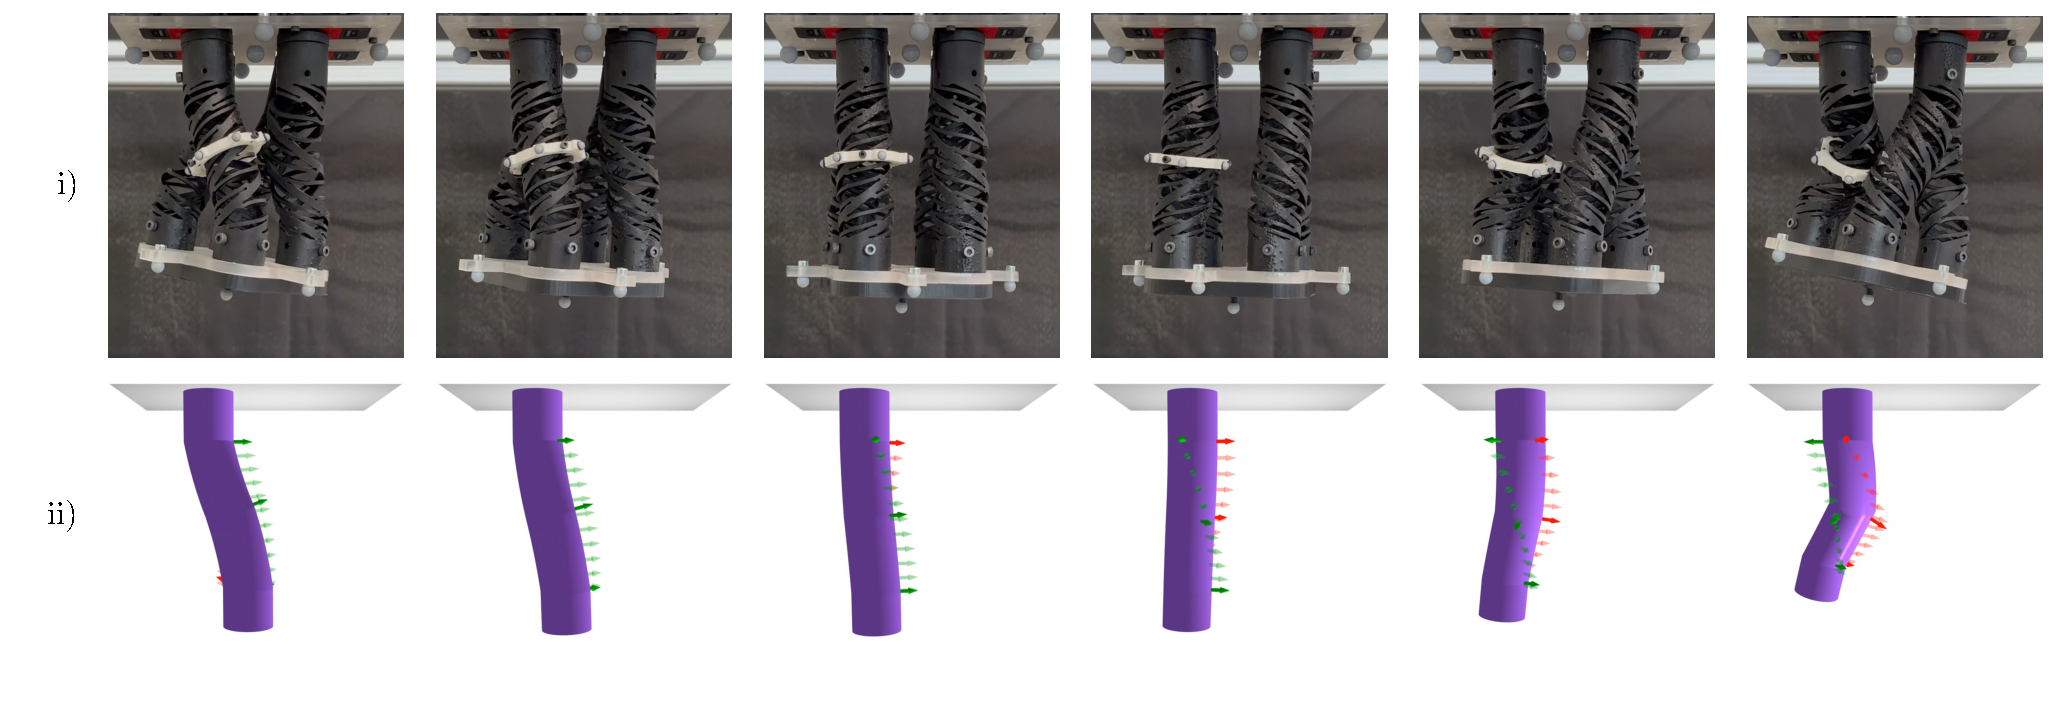
\includegraphics[width=0.9\textwidth]{hsamodel/figures/experiments_sequence_of_stills/experiment_twisting_inverse_kinematics_sequence_of_stills_v2_compressed.pdf}\label{fig:hsamodel:experiment_twisting_inverse_kinematics_sequence_of_stills}}
    
    \caption{Sequence of stills for a Lemniscate and a twisting trajectory. 
    % The numbers at the bottom signify the sample indices of the frames.
    \textbf{Top row i):} frames of a video recording of the HSA robot during the experiments. The shape of the front-left HSA rod is fitted using inverse kinematics and rendered in ii).
    \textbf{Bottom row ii):} Rendered shape of the HSA rod produced by evaluating the forward kinematics along the backbone length. The arrows with full opacity denote the ground-truth pose of three points along the HSA rod as measured by the motion capture system. The red arrow points along the local x-axis, and the green arrow along the local y-axis, respectively. The arrows with slight transparency represent poses along the backbone computed with the forward kinematics.
    We assume the last \SI{25}{mm} and \SI{20}{mm} at the proximal and distal end of the rod, respectively, to be rigid and therefore do not include them in the kinematic parametrization.
    % The white ring with the reflective motion capture markers points out the HSA rod (e.g. front-left), of which its shape is rendered in i).
    }\label{fig:hsamodel:experiment_inverse_kinematics_sequence_of_stills}
\end{figure*}

\subsubsection{Evaluation metrics}\label{ssub:hsamodel:hsa_rod_kinematics:evaluation_metrics}
We briefly introduce the metrics to quantify shape reconstruction accuracy by the proposed kinematic parametrization. 
We first define a \gls{RMSE} for comparing each ground-truth position $p_t^i \in \mathbb{R}^{3}, t \in \{1,\dots,n_t\}, i \in \{1,\dots,N\}$ to the position estimated by the kinematic model $\tilde{p}_t^i$ over a time period of $n_t$ steps
\begin{equation}\label{eq:hsamodel:translational_rmse}
    e_{\mathrm{p}} = \sqrt{\sum_{t = 1}^{n_\mathrm{t}} \sum_{i = 1}^{N} \frac{\left (\big\lVert \tilde{p}_t^i - p_t^i \big\rVert_2 \right )^2}{n_\mathrm{t} \, N}}  \in \mathbb{R}.
\end{equation}
% Next, we compute a rotational \gls{RMSE} in unit quaternion representation
% \begin{equation}
%     e_{\mathrm{quat}} = \sqrt{\sum_{t = 1}^{n_\mathrm{t}}  \sum_{i = 1}^{N} \frac{\left (\big\lVert \tilde{\varepsilon}_t^i - \varepsilon_t^i \big\rVert_2 \right )^2}{n_\mathrm{t} \, N}} \in \mathbb{R},
% \end{equation}
% where we use the Euclidean norm of the quaternion vector component $\varepsilon = \begin{pmatrix}\varepsilon_x & \varepsilon_y & \varepsilon_z \end{pmatrix}^\mathrm{T}$.
The rotational \glspl{RMSE} $e_{\mathrm{quat}}$ is computed analogue by substituting $p$ in \eqref{eq:hsamodel:translational_rmse} with the quaternion vector component $\varepsilon = \begin{pmatrix}\varepsilon_x & \varepsilon_y & \varepsilon_z \end{pmatrix}^\mathrm{T}$.
% Finally, we compute the relative rotation between $\tilde{R} \in \mathbb{3 \times 3}$ and $R \in \mathbb{3 \times 3}$ with $e_R = R \tilde{R}^\mathrm{T}$. 
Finally, we compute the XYZ Euler angle error as 
\begin{equation}
    e_\mathrm{eul} = \sqrt{\sum_{t = 1}^{n_\mathrm{t}} \sum_{i = 1}^{N} \frac{\left ( f_\vartheta(R_{t,i} \, \tilde{R}_{t,i}^\mathrm{T}) \right )^2}{n_\mathrm{t} \, N}} \in \mathbb{R}^3,
\end{equation}
where $f_\vartheta(\cdot)$ is the operator to compute the XYZ Euler angles $\vartheta = \begin{pmatrix}\alpha & \beta & \gamma \end{pmatrix}^\mathrm{T}$ from a rotation matrix $R \in SO(3)$.

% Relative rotation:
% \begin{equation}
%     R_T^{\tilde{T}} = R_s^\mathcal{B} \, \tilde{R}_{\mathcal{B}}^s
% \end{equation}

\subsubsection{Simulation results}\label{ssub:hsamodel:hsa_rod_kinematics:simulation_results}
%The suitability of the proposed, low-dimensional kinematic parametrization is first tested in simulation. 
%
We employ the higher dimensional \gls{HSA} robot simulator proposed in Section~\ref{sec:hsamodel:hsa_robot_simulation} to generate steady-state \gls{HSA} states. We use the same simulation parameters as in Section~\ref{sub:hsamodel:hsa_robot_simulation:motion_primitives}. This provides us with $25$ discrete poses along each of the four \glspl{HSA}.
Then, we perform differential inverse kinematics with a step size of $\lambda = 0.2$ to find an optimal configuration $q$ describing the shape of the \gls{HSA}. We choose a higher step size ($\lambda=1$) for regressing the twist strains.

For the kinematic model, we assume that the twist \& stretch strains are constant along the entire \gls{HSA} rod. The bend \& shear strains on the other hand are instead piece-wise constant across $n_\mathrm{S}$ segments. We evaluate the influence of the $n_\mathrm{S}$ parameter and test the performance of a kinematic model involving between $1$ and $5$ \gls{PCS} segments.

The results are in Fig.~\ref{fig:hsamodel:hsa_robot_simulation_kinematic_error_vs_number_of_PCS_segments}. While a kinematic model with a single \gls{CS} segment still works sufficiently well for the elongation and bending motion primitives, its performance deteriorates for any trajectories involving twisting. Instead, two segments of our model are sufficient to accurately represent the shape of the \gls{HSA}. 

% We perform an ablation study to identify which components of the kinematic parametrization are essential for accurately representing the shape of an \gls{HSA} rod. The results in Table~\ref{tab:hsamodel:kinematic_results_simulations} show that a parametrization neglecting the shear strains is not able to model the bending or twisting motion primitives. While one \gls{CS} segment is sufficient to represent the elongation and bending motion primitives, the performance sharply deteriorates on the twisting dataset. Finally, we conclude that considering the twist strain is not necessary and does not positively influence the performance significantly. 

% \begin{figure*}[hbt]
%     \centering
%     \subfigure[Positions]{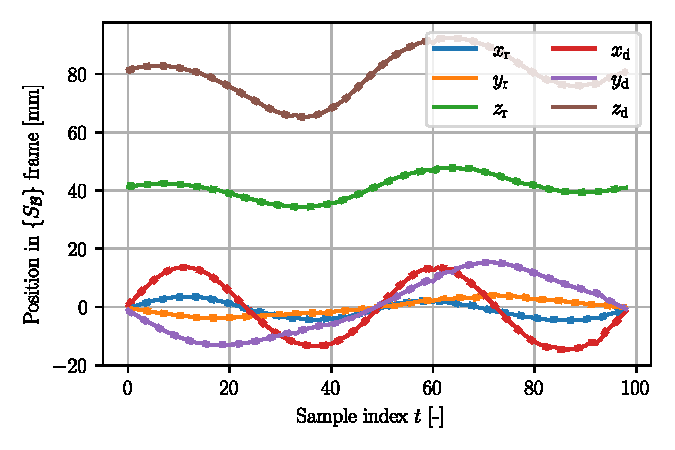
\includegraphics[width=0.49\textwidth]{hsamodel/figures/experiment_plots/inverse_kinematics_experimental_lemniscate_trajectory_positions_v4_cropped.pdf}\label{fig:hsamodel:inverse_kinematics_experimental_lemniscate_trajectory_positions}}
%     \subfigure[Euler XYZ angles]{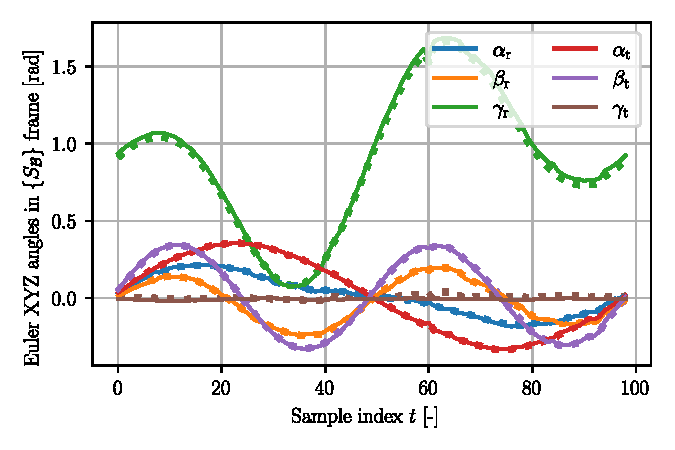
\includegraphics[width=0.49\textwidth]{hsamodel/figures/experiment_plots/inverse_kinematics_experimental_lemniscate_trajectory_euler_angles_v4_cropped.pdf}\label{fig:hsamodel:inverse_kinematics_experimental_lemniscate_trajectory_euler_angles}}
    
%     \caption{Kinematic model fitted on the experimental data of the Lemniscate actuation sequence. The solid lines denote the ground-truth poses with respect to the base frame $\{ S_{\mathcal{B}} \}$ collected by the motion capture system. The dotted lines represent the poses found when evaluating the kinematic model for the configuration $q$. This configuration was previously fitted through the means of differential inverse kinematics. The subscript $\mathrm{r}$ denotes the pose of the marker ring and the subscript $\mathrm{d}$ is connected to the pose of the distal end of the HSA rod. The kinematic model used to produce this results consists of two PCS~\cite{renda2018discrete} segments with the twist strains being neglected.}
% \end{figure*}

\subsubsection{Experimental results}\label{ssub:hsamodel:hsa_rod_kinematics:experimental_results}
In addition to the simulations, we also experimentally verify the kinematic model using an \gls{HSA} robot consisting of four closed rods 3D-printed via digital projection lithography from the flexible photopolymer resin Carbon FPU 50~\cite{truby2021recipe}. Each \gls{HSA} rod was printed to a length of $\bar{L} = \SI{101.6}{mm}$ and is independently actuated by DYNAMIXEL MX-28T servo motors.
% Right-handed and left-handed \glspl{HSA} are placed diagonally opposite of each other respectively.
As seen in Fig.~\ref{fig:hsamodel:experimental_setup}, we attach motion capture markers to several points on the robot to track the ground-truth pose information. Namely, we measure the pose of the motor base, the platform, and the midpoint of one of the right-handed \gls{HSA} rods (i.e. the front-left \gls{HSA} on the picture). Please note that we extract the rotation angle $\phi_0$ from the servo encoders directly. The robot is mounted at its base to a cubical cage of side length \SI{750}{mm} in platform-down configuration. Eight Optitrack Prime X 13 cameras are attached to the cage, tracking the reflective markers at \SI{30}{Hz}.

We actuate the robot from a workstation next-by with the control loop running at \SI{10}{Hz}. The control loop communicates motor position setpoints $u_\mathrm{d} \in \mathbb{R}^4$ to the servos. The inner control loop of the servos then applies the appropriate torques to guide the motors toward the desired position. As soon as the motors have reached their goal position, we wait for \SI{2}{s} to reach steady-state and then read out the pose measurements.

In Fig.~\ref{fig:hsamodel:experiment_inverse_kinematics_sequence_of_stills}, we show sequences of stills for the Lemniscate and twisting trajectory. The kinematic model used here assumes a constant twist strain along the entire rod and employs two \gls{PCS} segments to capture the remaining five strains. We see that except for extreme twisting states, e.g. the far right image in Fig.~\ref{fig:hsamodel:experiment_twisting_inverse_kinematics_sequence_of_stills}, the kinematic model is able to represent the complex \gls{HSA} shape very well.

In Tab.~\ref{tab:hsamodel:kinematic_results_experiments}, we quantitatively evaluate multiple kinematic models on the trajectories defined in \ref{ssub:hsamodel:hsa_rod_kinematics:actuation_sequences}. 
The first ($7$ DoF) and second ($11$ DoF) kinematic models are very similar as both assume constant twist and constant stretch along the entire \gls{HSA}. The other strains are contained in two \gls{PCS} segments in both cases. However, the first model exhibits much larger positional errors as it neglects shear strains, which are very important in \gls{HSA} robots but were not accounted for in the literature~\cite{garg2022kinematic}.
The third model provides the upper bound on the performance, as it has with $12$ comparatively many DoF and uses a piecewise formulation with two segments for all segments. 
% With two poses along the rod available in the experimental data, which results in 12 constraints, it should therefore be possible to perfectly fit this kinematic model to the provided pose information.

\section{Kinematic and dynamic modeling of planar HSA robots}\label{sec:hsamodel:planar_hsa_robot_model}
In this section, we present a control-oriented, minimalistic kinematic and dynamic model for planar \gls{HSA} robots. We first introduce the kinematic model of the robot and then derive the dynamic model in Euler-Lagrangian form. We then verify the predictive capabilities of the dynamic model on unseen trajectories.

\subsection{Kinematic model}\label{sub:hsamodel:planar_hsa_robot_model:kinematics}
Following the discrete Cosserat approach~\cite{renda2018discrete}, we characterize the configuration space of the virtual backbone by assuming a \gls{CS} model
$\presub{\mathcal{V}}{\xi}(t) = \begin{bmatrix}\presub{{\mathcal{V}}}{\kappa}_\mathrm{be} & \presub{{\mathcal{V}}}{\kappa}_\mathrm{sh} & \presub{{\mathcal{V}}}{\sigma}_\mathrm{ax}\end{bmatrix}^\mathrm{T} = \mathbb{I}_3 \, q(t) \in \mathbb{R}^3$, where $\kappa_\mathrm{be}$, $\sigma_\mathrm{sh}$, and $\sigma_\mathrm{ax}$ denote the bending, shear, and axial strain respectively.
% We describe the configuration $q$ of the virtual backbone using a planar constant strain model~\cite{renda2018discrete} with $q(t) = \presub{\mathcal{V}}{\xi}(t) = \begin{bmatrix}\presub{\mathcal{V}}{\kappa}_\mathrm{be} & \presub{\mathcal{V}}{\kappa}_\mathrm{sh} & \presub{\mathcal{V}}{\sigma}_\mathrm{ax}\end{bmatrix}^\mathrm{T}$ consisting of bending, shear, and axial strains.  
% The $\presub{\mathcal{V}}{\text{subscript}}$ denotes variables corresponding to the virtual backbone. 
% (denoted with a $\presub{\mathcal{P}}{\text{subscript}}$)
Given $q$, the pose $\chi = \begin{bmatrix}
    p_x & p_y & \theta
\end{bmatrix}^\mathrm{T} \in SE(2)$, and a point coordinate along the backbone $s \in [0, l^0]$, the forward and inverse kinematics are provided in closed form as
\begin{equation}\label{eq:hsamodel:planar_hsa_robot_model:kinematics}
    \chi = \pi(q, s) = \begin{bmatrix}
        \sigma_\mathrm{sh} \, \frac{\mathrm{s}_\mathrm{be}}{\kappa_\mathrm{be}} + \sigma_\mathrm{ax} \, \frac{\mathrm{c}_\mathrm{be}-1}{\kappa_\mathrm{be}}\\
        \sigma_\mathrm{sh} \, \frac{1-\mathrm{c}_\mathrm{be}}{\kappa_\mathrm{be}} + \sigma_\mathrm{ax} \, \frac{\mathrm{s}_\mathrm{be}}{\kappa_\mathrm{be}}\\
        \kappa_\mathrm{be} \, s
    \end{bmatrix},
    \qquad
    q = \varrho(\chi, s) 
    = \frac{\theta}{2s} \: \begin{bmatrix}
        2\\
        p_y - \frac{p_x \, \mathrm{s}_\theta}{\mathrm{c}_\theta-1}\\
        -p_x - \frac{p_y \, \mathrm{s}_\theta}{\mathrm{c}_\theta-1}
   \end{bmatrix},
\end{equation}
where we use the shorthand notations $\mathrm{s}_\mathrm{be} = \sin(\kappa_\mathrm{be}s)$, $\mathrm{c}_\mathrm{be} = \cos(\kappa_\mathrm{be}s)$, $\mathrm{s}_\theta = \sin(\theta)$, and $\mathrm{c}_\theta = \cos(\theta)$.
Furthermore, the forward kinematics of the physical rods $\mathcal{P}_i, \, i \in \{1, 2\}$ can be derived by first following the transformations of the virtual backbone and then adding a local translation $[\pm r_{\mathrm{off}},0]^\mathrm{T}$ with $r_\mathrm{off}$ being the offset distance from the virtual backbone to the centerline of the \gls{HSA} rod. 
After closing the kinematic chain, we identify a mapping $\beta_i: \presub{\mathcal{V}}{\xi} \rightarrow \presub{\mathcal{P}_i}{\xi}$ from the strains of the virtual backbone to the strains in the physical rods: $\beta_i(\presub{\mathcal{V}}{\xi}) = \begin{bmatrix}
    \presub{\mathcal{V}}{\kappa}_\mathrm{be}, & \presub{\mathcal{V}}{\sigma}_\mathrm{sh}, & \presub{\mathcal{V}}{\sigma}_\mathrm{ax} \pm r_{\mathrm{off}}  \presub{\mathcal{V}}{\kappa}_\mathrm{be}
\end{bmatrix}^\mathrm{T}$.
% 
Analog to the dynamic simulator in Sec.~\ref{sec:hsamodel:hsa_robot_simulation}, we model the auxetic trajectory of the \glspl{HSA} by coupling the rest length $\tilde{l}_i$ to the twist strain $\kappa_{\mathrm{tw},i}$ of the $i$th \gls{HSA} rod: $\tilde{l}_i = (1 + \epsilon_i) l^0 = (1 + h_i C_\epsilon \kappa_{\mathrm{tw},i})$ where $l^0$ is the printed length of the rod and $C_\epsilon$ a positive constant.
The handedness $h_i \in \{-1, 1\}$ describes if positive or negative twist angles are needed to elongate the closed \gls{HSA}.
For a given vector of rod twist angles $\phi \in \mathbb{R}^2$ and after defining $\phi_{i}^+ = h_i \phi_i$, the elongation of the $i$th rod is then $\epsilon_i = C_\epsilon \frac{\phi_{i}^+}{l^0}$.
% As we can measure the twist angle $\phi \in \mathbb{R}^2$ of the rods by querying the encoders of the electric motors, the modification of the rest length is then denoted as $\epsilon_i = C_\epsilon h_i \frac{\phi_i}{l_i^0}$.
% The handedness $h_i \in \{-1, 1\}$ describes if positive or negative twist angles need to be applied to cause an elongation of the closed \glspl{HSA}.


\subsection{Dynamic model}\label{sub:hsamodel:planar_hsa_robot_model:dynamics}
We aim to devise a dynamic model in the Euler-Lagrange form
$M(q) \Ddot{q} + C(q,\dot{q})\dot{q} + G(q) + K (q - q^0) + D \dot{q} = \alpha(q,\phi),$
where $M(q),C(q,\dot{q}),K,D \in \mathbb{R}^{3 \times 3}$ are the inertia, Coriolis (derived with Christoffel symbols), elastic and damping matrices respectively. $q^0 \in \mathbb{R}^3$ captures the rest configuration. The terms $G(q)$ and $\alpha(q,\phi) \in \mathbb{R}^3$ describe the gravitational and actuation forces acting on the generalized coordinates.
The state of the robot at time $t$ can be therefore described by $x(t) = \begin{bmatrix}
    q^\mathrm{T}(t) & \dot{q}^\mathrm{T}
\end{bmatrix}^\mathrm{T} \in \mathbb{R}^6$.
The inertia matrix is found by following the standard procedure of integrating mass and rotational inertia along the \gls{HSA} rods~\cite{della2023model}. Additionally, we consider the inertial contribution of the platform mounted to the distal end of the robot.
% The Coriolis matrix can then be derived using Christoffel symbols.
% Next, we consider the elasticity of the robot. 
Under the small strain assumption, the elastic forces of the $i$th \gls{HSA} rod can be modeled as
\begin{equation}
    \presub{\mathcal{P}}{\tau}_{\mathrm{K},i} = 
    % \begin{bmatrix}
    %     \mathcal{I}_\mathrm{be} E_i(\phi_i) & S_{\mathrm{be},\mathrm{sh},i} & 0\\
    %     S_{\mathrm{be},\mathrm{sh},i} & \frac{4}{3}A G_i(\phi_i) & 0\\
    %     0 & 0 & A E_i(\phi_i)
    % \end{bmatrix} 
    \begin{bmatrix}
        S_{\mathrm{be},i}(\phi_i) & S_{\mathrm{be},\mathrm{sh}} & 0\\
        S_{\mathrm{be},\mathrm{sh}} & S_{\mathrm{sh},i}(\phi_i) & 0\\
        0 & 0 & S_{\mathrm{ax},i}(\phi_i)
    \end{bmatrix} 
    \, \left ( \begin{bmatrix}
        \presub{\mathcal{P}_i}{\kappa}_\mathrm{be}\\ \presub{\mathcal{P}_i}{\sigma}_\mathrm{sh}\\ \presub{\mathcal{P}_i}{\sigma}_\mathrm{ax}
    \end{bmatrix} - \begin{bmatrix}
        \kappa_\mathrm{be}^0\\ \sigma_\mathrm{sh}^0\\ \sigma_\mathrm{ax}^0 + \epsilon_i (\phi_i)
    \end{bmatrix} \right ),
\end{equation}
where $\presub{\mathcal{P}_i}{\xi}^0 = \begin{bmatrix}\kappa_\mathrm{be}^0 & \sigma_\mathrm{sh}^0 & \sigma_\mathrm{ax}^0\end{bmatrix}^\mathrm{T}$ denotes the rest strain,
$S_{\mathrm{be},i}(\phi_i)$, $S_{\mathrm{sh},i}(\phi_i)$, $S_{\mathrm{ax},i}(\phi_i)$ are the bending, shear, and axial stiffnesses which are defined as linear functions with respect to the twist angle of the rod $\phi_i$~\cite{good2022expanding, stolzle2023modelling}:
\begin{equation}
    S_{\mathrm{be},i}(\phi_i) = \hat{S}_{\mathrm{be}} + C_{\mathrm{S}_\mathrm{be}} \, \phi_{i}^+,
    \quad
    S_{\mathrm{sh},i}(\phi_i) = \hat{S}_{\mathrm{sh}} + C_{\mathrm{S}_\mathrm{sh}} \, \phi_{i}^+,
    \quad 
    S_{\mathrm{ax},i}(\phi_i) = \hat{S}_{\mathrm{ax}} + C_{\mathrm{S}_\mathrm{ax}} \, \phi_{i}^+.
\end{equation}
The coefficient $S_{\mathrm{be},\mathrm{sh}}$ accounts for the elastic coupling between the bending and the shear strain. 
% and $A$, $\mathcal{I}_\mathrm{be}$ the cross-sectional area and the second area moment of inertia respectively. The elastic modulus of closed \glspl{HSA} can be modeled with a linear function of the twist strain: $E_i(\phi_i) = E^0 + C_\mathrm{E} h_i \frac{\phi_i}{l_i^0}$~\cite{good2022expanding, stolzle2023modelling}. $G_i(\phi_i)$ is formulated in an analog fashion.
Subsequently, we project the forces into the virtual backbone by premultiplying with $J_\beta^\mathrm{T} = \frac{\partial \beta}{\partial q}^\mathrm{T}$ and then sum the contribution of all rods.
Finally, we group all terms depending on the control input $\phi$ in $\alpha(q,\phi)$ and everything else in $K$.
After modeling the dissipative forces in each \gls{HSA} as $\mathrm{diag}(\zeta_\mathrm{be}, \zeta_{\mathrm{sh}}, \zeta_{\mathrm{ax}}) \, \presub{\mathcal{P}_i}{\dot{\xi}}$, we derive the damping matrix in configuration space as $D = \sum_{i=1}^{2} J_{\beta,i}^\mathrm{T} \, \mathrm{diag}(\zeta_\mathrm{be}, \zeta_{\mathrm{sh}}, \zeta_{\mathrm{ax}}) \, J_{\beta,i} = 2 \, \mathrm{diag}\left ( (\zeta_\mathrm{be} + r_\mathrm{off}^2 \, \zeta_\mathrm{ax} ), \zeta_{\mathrm{sh}}, \zeta_{\mathrm{ax}} \right)$.
% \begin{equation}
%     D = \sum_{i=1}^{2} J_{\beta,i}^\mathrm{T} \, \mathrm{diag}(\zeta_\mathrm{be}, \zeta_{\mathrm{sh}}, \zeta_{\mathrm{ax}}) \, J_{\beta,i} = 2 \, \mathrm{diag}\left ( (\zeta_\mathrm{be} + r_\mathrm{off}^2 \, \zeta_\mathrm{ax} ), \zeta_{\mathrm{sh}}, \zeta_{\mathrm{ax}} \right)
%     % \begin{bmatrix}
%     %     (\zeta_\mathrm{be} + r_\mathrm{off}^2 \, \zeta_\mathrm{ax} ) & 0 & 0\\
%     %     0 & \zeta_{\mathrm{sh}} & 0 \\
%     %     0 & 0 & \zeta_{\mathrm{ax}}
%     % \end{bmatrix}.
% \end{equation}
We open-source the derivation of the Euler-Lagrangian dynamics and a JAX implementation of a simulator based on them on GitHub\footnote{\url{https://github.com/tud-phi/jax-soft-robot-modelling}}.

\begin{figure}[ht]
    \centering
    \subfigure[FPU: End-effector pose]{\includegraphics[width=0.48\columnwidth, trim={10, 10, 10, 10}]{hsamodel/figures/model_verification/20230621_183620_model_verification_chiee.pdf}\label{fig:hsamodel:planar_hsa_robot_model:model_verification:fpu:chiee}}
    \subfigure[FPU: Configuration]{\includegraphics[width=0.48\columnwidth, trim={10, 10, 10, 10}]{hsamodel/figures/model_verification/20230621_183620_model_verification_q.pdf}\label{fig:hsamodel:planar_hsa_robot_model:model_verification:fpu:q}}\\
    \subfigure[EPU: End-effector pose]{\includegraphics[width=0.48\columnwidth, trim={10, 10, 10, 10}]{hsamodel/figures/model_verification/20230927_150452_model_verification_chiee.pdf}\label{fig:hsamodel:planar_hsa_robot_model:model_verification:epu:chiee}}
    \subfigure[EPU: Configuration]{\includegraphics[width=0.48\columnwidth, trim={10, 10, 10, 10}]{hsamodel/figures/model_verification/20230927_150452_model_verification_q.pdf}\label{fig:hsamodel:planar_hsa_robot_model:model_verification:epu:q}}
    \caption{Verification of the system model and the identified system parameters on an unseen trajectory with the HSA being randomly actuated through a GBN sequence: the solid line denotes the actual trajectory. In contrast, the dashed line visualizes the trajectory simulated with the system model. We report results for both FPU and EPU-based \glspl{HSA}.}\label{fig:hsamodel:planar_hsa_robot_model:model_verification}
\end{figure}

\subsection{Model verification}\label{sub:hsamodel:planar_hsa_robot_model:model_verification}

\subsubsection{Experimental setup}\label{ssub:hsamodel:planar_hsa_robot_model:model_verification:experimental_setup}
We evaluate the planar \gls{HSA} model experimentally.
The material choice of the \gls{HSA} is crucial and has a significant influence on the resulting mechanical characteristics of the robot  (e.g., blocked force, holding torque, bending stiffness, etc.)~\cite{truby2021recipe}. Furthermore, specific material requirements are dictated by the nature of the design of the \gls{HSA} rod. The structure of the metamaterial is made of struts connected by living hinges. These living hinges must be thin, flexible, and accommodate high strains~\cite{truby2021recipe}.
In order to ensure that the system model is effective and suitable for a range of different materials, we decided to conduct the experimental verification on \glspl{HSA} 3D-printed via digital projection lithography either using the photopolymer resin Carbon FPU 50~\cite{carbon:fpu50} (stiffer) or the elastomeric polyurethane EPU 40 resin~\cite{carbon:epu40} (softer).

The Dynamixel MX-28 servo motor are set to use position control mode. % which runs a cascaded PID control loop on the motor current.
% The robot is mounted platform-down on a cage on which we have also attached eight Optitrack PrimeX 13 cameras. The motion capture system can track the SE(3) pose of both the base and the platform at a sampling rate of \SI{200}{Hz}. 
The robot is mounted platform-down on a cage with an Optitrack motion capture system, which measures the SE(3) pose of the platform at \SI{200}{Hz}.
Our algorithms run within a ROS2 framework\footnote{\url{https://github.com/tud-phi/ros2-hsa}}. % First, we project the pose measurements into the plane of actuation. Then, we evaluate the coordinate transformation between platform and base and run the closed-form inverse kinematics introduced in \eqref{eq:hsamodel:planar_hsa_robot_model:kinematics}. We store in memory the last \textcolor{orange}{ten} configuration measurements, fit a cubic spline to each configuration variable using the \emph{Derivative} package~\cite{kaptanoglu2022pysindy}, and then differentiate the spline function to gather $\dot{q}(t)$.
% ~\footnote{\url{https://github.com/tud-phi/ros2-hsa}}
% ~\cite{kaptanoglu2022pysindy}
% Our algorithms run within a ROS2 framework. 
The pose measurements are first projected into the plane of actuation and serve as an input to the closed-form inverse kinematics introduced in \eqref{eq:hsamodel:planar_hsa_robot_model:kinematics}. 
% We use a Savitzky-Golay filter with a window duration of $\SI{0.1}{s}$ to numerically differentiate $\chi_\mathrm{ee}(t)$, $q(t)$ and gather with that $\dot{\chi}_\mathrm{ee}(t)$ and $\dot{q}(t)$.
% We fit a cubic spline to the last $16$ configuration measurements and differentiate~\cite{kaptanoglu2022pysindy} to gather $\dot{q}(t)$.

\subsubsection{System identification}\label{ssub:hsamodel:planar_hsa_robot_model:model_verification:system_identification}
Next, we strive to identify the parameters used in our dynamic model.
We assume the robot's geometric and mass density properties to be known or easily measurable. % Therefore, we are left with having to identify the elastic and damping characteristics of the robot.
As knowledge about the damping coefficients is not required by the control law, only the experimental identification of elongation and stiffness characteristics remains.
For this, we measure the response of the system to step and staircase actuation sequences. Afterward, the parameters are regressed using least squares. % first in a static, pure elongation setting and then gradually also on dynamic sequences involving bending and shear.
For the FPU-based robot, we identify $C_\varepsilon^\mathrm{FPU}=\SI{0.0079}{m \per rad}$, $S_\mathrm{be}^\mathrm{FPU} = -2.5 \cdot 10^{-5} + 3.9 \cdot 10^{-7} \, \frac{\phi_i^+}{l^0} \si{Nm^2}$, $S_\mathrm{sh}^\mathrm{FPU} = 0.043 + 0.0029 \, \frac{\phi_i^+}{l^0} \si{N}$, $S_\mathrm{ax}^\mathrm{FPU} = 0.74 + 0.0098 \, \frac{\phi_i^+}{l^0} \si{N}$, and $S_\mathrm{b,sh}^\mathrm{FPU} = -5.0 \cdot 10^{-4} \si{Nm \per rad}$ where $l^0 = \SI{0.059}{m}$. 
Furthermore, we regress $C_\varepsilon^\mathrm{EPU}=\SI{0.0098}{m \per rad}$, $S_\mathrm{be}^\mathrm{EPU} = 5.7 \cdot 10^{-4} -9.7 \cdot 10^{-6} \, \frac{\phi_i^+}{l^0} \si{Nm^2}$, $S_\mathrm{sh}^\mathrm{EPU} = 0.59 - 0.00047 \, \frac{\phi_i^+}{l^0} \si{N}$, $S_\mathrm{ax}^\mathrm{EPU} = 5.7 + 0.015 \, \frac{\phi_i^+}{l^0} \si{N}$, and $S_\mathrm{b,sh}^\mathrm{EPU} = -\SI{0.00048}{Nm \per rad}$ for the EPU \glspl{HSA} which have the same length as the FPU \glspl{HSA}.
Finally, we identify the axial rest strain $\sigma_\mathrm{ax}^0$ before the start of each experiment.
We notice that the EPU-based HSA robot is approximately one order of magnitude more flexible than the FPU-based robot.

\subsubsection{Results}\label{ssub:hsamodel:planar_hsa_robot_model:model_verification:results}
We verify the accuracy of the proposed system model and the identified parameters on trajectories unseen during system identification. We generate the trajectories by actuating the robot with a \gls{GBN}~\cite{tulleken1990generalized} sequence with a settling time of \SI{0.5}{s} and at each time step $k$ randomly sample $\phi(k) \sim \mathcal{U}(0, \phi_\mathrm{max})$.
We simulate the model evolution with a Dormand-Prince 5(4) integrator and a time step of \SI{0.1}{ms}.
Fig.~\ref{fig:hsamodel:planar_hsa_robot_model:model_verification:fpu:chiee} shows the model exhibiting excellent accuracy for representing the behavior of FPU-based \gls{HSA} robots.
We observe more significant errors in the shear estimate for EPU-based \gls{HSA} robots in Fig.\ref{fig:hsamodel:planar_hsa_robot_model:model_verification:epu:q}. Specifically, the \gls{CS} model no longer seems sufficient for capturing the robot's shape, particularly for larger bending angles. Therefore, we suggest for future work to employ kinematic models with more \gls{DOF} such as \gls{PCS} as proposed, for example, in Sec.~\ref{sec:hsamodel:hsa_rod_kinematics} or \cite{renda2018discrete}.

\section{Conclusion}\label{sec:hsamodel:conclusion}
%
This chapter provided solutions for the first time for modeling the kinematics and the dynamics of electrically-actuated continuum soft robots based on Handed Shearing Auxetics.
%
We have shown that coupling the twist strains to rest lengths can allow simulators based on the discrete Cosserat rod theory. %to capture the behaviour of both single \glspl{HSA} and entire \glspl{HSA} robots.
While the proposed linear approximation of the auxetic trajectory works well for closed \glspl{HSA} within a bounded motion range, future work shall derive a more general model also applicable for semi-closed and open \glspl{HSA}~\citep{good2022expanding}.
% Namely, we were able to invoke all motion primitives: elongation, bending, and twisting.
Furthermore, we have proposed the \gls{SPCS} kinematic model that can express the shape of \glspl{HSA} with $11$ \glspl{DOF}.
Fitting this kinematic model to the experimental results showed a very good match for representing the shape of the \glspl{HSA}. In particular, for large actuation magnitudes within the twisting motion primitive, the \glspl{HSA} leave the auxetic trajectory and seem to experience buckling behavior. For this case, the \gls{SPCS} model is not accurate anymore.
% Our simulations and the experimental campaign showed that the twist \& stretch strains can be assumed to be constant along the entire \gls{HSA} while at least $2$ \gls{CS} segments are necessary to capture the bend \& shear strains during the twisting motion primitive. Furthermore, the magnitude of shear strains is significant during bending and twisting and cannot be neglected. %, as it was done in previous work~\citep{garg2022kinematic}.
Finally, we presented a control-oriented dynamic model for planar \gls{HSA} robots and verified it experimentally.
The conducted experiments gave us deep insights into the particular characteristics of \glspl{HSA} and how well our model is able to capture them. We see excellent agreement for predicting the dynamical behavior of \gls{HSA} robots made of FPU material.
We observed the time lag of the model to be larger for EPU-based robots, as seen in Fig.~\ref{fig:hsamodel:planar_hsa_robot_model:model_verification:epu:chiee}. This probably is the result of the hysteresis characteristics of \glspl{HSA}~\citep{good2022expanding}.
For EPU-based \glspl{HSA} robots, we observe that the model does not fully capture the shear dynamics.



\section*{Afterword}
This chapter presented approaches for representing the kinematics and dynamics of \gls{HSA} rods in the general case. Additionally, we introduced the first low-dimensional kinematic parameterizations and control-oriented dynamical models for planar \gls{HSA} robots.
Next, Chapter~\ref{chp:hsacontrol} will focus on leveraging the models proposed in this chapter for model-based control of planar \gls{HSA} robots.
Namely, this includes the development of stable and effective configuration-space PID+feedforward and task-space impedance controllers.
Subsequently, Chapter~\ref{chp:braincontrol} will develop a \gls{BCI} strategy for guiding soft robots, and specifically \gls{HSA} robots, using motor imagery in a safe and compliant fashion.
\chapter{Model-based Control of Handed Shearing Auxetics (HSA) Robots}
\label{chp:hsacontrol}

\begin{abstract}
    Parallel robots based on Handed Shearing Auxetics (HSAs) can implement complex motions using standard electric motors while maintaining the complete softness of the structure, thanks to specifically designed architected metamaterials.
    However, their control is especially challenging due to varying and coupled stiffness, shearing, non-affine terms in the actuation model, and underactuation. In this chapter, we present a model-based control strategy for planar HSA robots enabling regulation in task space. 
    We formulate equations of motion, show that they admit a collocated form, and design a P-satI-D feedback controller with compensation for elastic and gravitational forces. 
    We experimentally identify and verify the proposed control strategy in closed loop.
\end{abstract}

\blfootnote{This chapter is partly based on 
    \begin{itemize}
        \item[\faFileTextO] ~\emph{\textbf{M. Stölzle}, D. Rus, and C. Della Santina (2023, December). An Experimental Study of Model-based Control for Planar Handed Shearing Auxetics Robots. In Experimental Robotics: The 18th International Symposium. Springer}~\cite{stolzle2024experimental}.
        \item[\faFileTextO] ~\emph{\textbf{M. Stölzle}*, S. S. Baberwal*, D. Rus, S. Coyle, and C. Della Santina (2024). Guiding Soft Robots with Motor-Imagery Brain Signals and Impedance Control. In Proceedings of The 2024 IEEE 7th International Conference on Soft Robotics (RoboSoft) (pp. 1-8). IEEE. \textbf{Best Paper Award}~\cite{stolzle2024guiding}}.
    \end{itemize}
}


%% Start the actual chapter on a new page.
\newpage

\section{Introduction}
% The deformability, adaptiveness, and compliance of invertebrates serve as an inspiration for continuum soft robots.
% While serial continuum soft robots have been intensively investigated in recent years~\cite{della2023model}, parallel soft robots~\cite{hughes2020extensible, zhang2020modeling} are less studied despite exhibiting exciting properties such as an improved stiffness-to-weight ratio. 
% One recent development in this field is robots based on \glspl{HSA}~\cite{truby2021recipe, kaarthik2022motorized, stolzle2024guiding} in which multiple \gls{HSA} rods are connected at their distal end through a rigid platform. 
% Twisting of the proximal end of an \gls{HSA} % with an electric actuator 
% causes the rod to elongate and enables complex motion primitives in 3D space.
Recent work has investigated proprioception~\cite{zhang2022vision}, the mechanical characterization~\cite{good2022expanding}, simulation~\cite{stolzle2023modelling}, and kinematic modeling~\cite{garg2022kinematic, stolzle2023modelling} of \gls{HSA} robots but control has yet to be tackled.
% Still, the task of control is still unsolved as \textcolor{orange}{prior work} and solutions need to be developed on how to deal with the challenges of underactuation and changing stiffness properties. 
In this work, we make a first step towards achieving task-space control by designing model-based regulators for planar motions. Our approach considers essential characteristics of \gls{HSA} robots, such as underactuation, shear strains, and varying stiffness. % and thus can serve as a building block for future research.

In Chapter~\ref{chp:hsamodel}, we derived a dynamic model for planar \gls{HSA} in Euler-Lagrange form and experimentally verified it.
We notice that the resulting planar dynamics are underactuated and that the actuation forces are non-affine with respect to the control inputs, which are the motor angles. The latter is a peculiarity of these systems, rarely observed in other robots.
Based on the model knowledge, we propose in this chapter two control strategies for planar \gls{HSA} robots capable of regulating the end-effector towards a desired position in task-space.
The first strategy, as shown in Fig.~\ref{fig:hsacontrol:configuration_space_regulation:block_scheme_closed_loop_control}, performs steady-state planning to identify an admittable configuration and steady-state control input matching the desired end-effector position and then subsequently applies a P-satI-D feedback controller~\cite{pustina2022p} on the collocated form~\cite{pustina2024input} of the system dynamics.
The second strategy, as shown in Fig.~\ref{fig:hsacontrol:task_space_impedance_control:block_scheme_closed_loop_control}, directly regulates the end-effector position using a Cartesian impedance controller that fully preserves the softness of the robot.

In summary, we state our contributions as (i) a provably stable model-based control strategy for guiding the end-effector of the robot towards a desired position in Cartesian space with a configuration-space controller that combines an integral-saturated PID with a potential shaping feedforward term, (ii) a Cartesian impedance controller that allows combining the passive compliance of the \gls{HSA} robot with active compliance in the control strategy and (iii) extensive experimental verification of both control strategies. 
A video accompanies this chapter explaining the methodology and displaying video recordings of the control experiments\footnote{\url{https://youtu.be/7PgKnE_MOsY}}.


%Structure
%\begin{enumerate}
%    \item Why soft robots
%    % \item Parallel soft robots have not been widely tested out,  have interesting characteristics such as higher bending stiffness with low weight
%    \item HSAs have this special mechanism in which the motors acts throught he stiffness of the hsa on the robot shape
%    \item Control has only been performed with PID, no model-based control. Problem of underactuation needs to be solved. Way to deal with changing stiffness characteristics
%\end{enumerate}
%
%Our contributions
%\begin{itemize}
%    \item Closed-form inverse kinematics for planar continuum robots modelled using PCS
%    \item An Euler-Lagrangian model for the dynamics of HSA robots, which is then also verified experimentally 
%    \item Proposal of a control strategy involving mapping from task-space to configuration-space and PID controller respecting the underactuation
%    \item Experiments involving Model-based regulation of HSA robots
%\end{itemize}
\section{Configuration Space Regulation}\label{sec:hsacontrol:configuration_space_regulation}
In this Section, we derive a model-based control strategy in configuration space for achieving setpoint regulation that combines an integral-saturated PID controller with a potential-shaping feedforward term. We first introduce the dynamical model of the planar \gls{HSA} robot and then present the control strategy.
Subsequently, we present a steady-state planning procedure to identify admittable configurations and matching steady-state actuation.
Finally, we experimentally verify the proposed control strategy in closed loop.

\subsection{Background: Dynamical model}\label{sub:hsacontrol:model}
As introduced in Sec.~\ref{sec:hsamodel:planar_hsa_robot_model}, the state of a planar \gls{HSA} robot at time $t$ can be therefore described by $x(t) = \begin{bmatrix}
    q^\mathrm{T}(t) & \dot{q}^\mathrm{T}
\end{bmatrix}^\mathrm{T} \in \mathbb{R}^6$, where $\kappa_\mathrm{be}$, $\sigma_\mathrm{sh}$, and $\sigma_\mathrm{ax}$ denote the bending, shear, and axial strain respectively.
The dynamical model is then given in Euler-Lagrange form as
\begin{equation}\label{eq:hsacontrol:dynamics}
    M(q) \Ddot{q} + C(q,\dot{q})\dot{q} + G(q) + K (q - q^0) + D \dot{q} = \alpha(q,\phi),
\end{equation}
where $M(q),C(q,\dot{q}),K,D \in \mathbb{R}^{3 \times 3}$ are the inertia, Coriolis, elastic and damping matrices, respectively. $q^0 \in \mathbb{R}^3$ captures the rest configuration. The terms $G(q)$ and $\alpha(q,\phi) \in \mathbb{R}^3$ describe the gravitational and actuation forces acting on the generalized coordinates.
We provide examples in Fig.~\ref{fig:hsacontrol:kinematics:workspace} of the operational workspace that can be achieved with this kinematic model.
We stress that (a) the derived dynamical model is not affine in the control input and (b) the system is underactuated.

\begin{figure}[ht]
    \centering
    \subfigure[Blockscheme]{\includegraphics[width=0.62\textwidth]{hsacontrol/figures/control_schemes/configuration_space_regulation/control_scheme_v4_cropped.pdf}\label{fig:hsacontrol:configuration_space_regulation:block_scheme_closed_loop_control}}
    \subfigure[Operational workspace]{\includegraphics[width=0.37\columnwidth, trim={7, 7, 7, 7}]{hsacontrol/figures/kinematics/fpu_operational_workspace.pdf}\label{fig:hsacontrol:kinematics:workspace}}
    \caption{\textbf{Panel (a):} Block scheme for configuration-space regulator: we plan the steady-state behavior such that the end-effector matches the given desired position $p_\mathrm{ee}^\mathrm{d}$. The outputs of this planning are the steady-state actuation $\phi^\mathrm{ss}$ and a suitable end-effector orientation $\theta_\mathrm{ee}^\mathrm{d}$. After leveraging inverse kinematics to identify the desired and current configuration, $q$ is mapped into a collocated form where the inputs are decoupled. Finally, we use a P-satI-D feedback controller on the actuation coordinates $\varphi$. \textbf{Panel (b):} Visualization of the operational workspace of a planar HSA robot consisting of FPU rods. The colored area within the black dashed borders represents the positions the end-effector (visualized as a dot) can reach. The coloring denotes the mean magnitude of actuation (i.e., twisting of the rods). Furthermore, we plot three sample configurations: the unactuated straight configuration $q = [0, 0, 0]^\mathrm{T}$ (blue), maximum clockwise bending $q = [\SI{-11.2}{rad \per m}, 0.08, 0.30]^\mathrm{T}$ (red), and maximum counter-clockwise bending $q = [\SI{11.2}{rad \per m}, -0.08, 0.30]^\mathrm{T}$ (green).}
\end{figure}

\subsection{Control strategy}\label{sub:hsacontrol:configuration_space_regulation:control_strategy}

Our goal is to control the end-effector, which is defined as the distal surface of the platform, to a desired position in Cartesian space $p_\mathrm{ee}^\mathrm{d} \in \mathbb{R}^2$. 
However, the mapping into configuration space is not trivial as we do not know which end-effector orientation $\theta_\mathrm{ee}$ is feasible at steady-state. 
To tackle this challenge, we perform steady-state planning identifying admittable configurations $q^\mathrm{d}$ and matching steady-state actuations $\phi^\mathrm{ss}$, which allow the robot's end-effector to statically remain at $p_\mathrm{ee}^\mathrm{d}$. More details on the used planning procedure can be found in Section~\ref{sub:hsacontrol:experiments:steady_state_planning}.

\begin{figure}[hbt]
    \centering
    \subfigure[$\alpha(q, \phi)$ for FPU]{\includegraphics[width=0.80\columnwidth]{hsacontrol/figures/actuation_characteristics/nonlinear_alpha_fpu_cropped.pdf}}\\
    \subfigure[$\alpha(q, \phi)$ for EPU]{\includegraphics[width=0.80\columnwidth]{hsacontrol/figures/actuation_characteristics/nonlinear_alpha_epu_cropped.pdf}}\\
    \subfigure[$\alpha(q^\mathrm{ss}, \phi^\mathrm{ss}) + A_{\phi^\mathrm{ss}}(q) \, (\phi - \phi^\mathrm{ss})$ for EPU]{\includegraphics[width=0.80\columnwidth]{hsacontrol/figures/actuation_characteristics/linearized_alpha_epu_cropped.pdf}}\\
    \subfigure[$A_{\varphi} \, (\phi - \phi^\mathrm{ss})$]{\includegraphics[width=0.80\columnwidth]{hsacontrol/figures/actuation_characteristics/actuation_coordinates_cropped.pdf}}\\
    \caption{Mapping of actuation $\phi \in \mathbb{R}^2$ to configuration-space torques $\tau \in \mathbb{R}^3$ for planar \gls{HSA} robots. The first two rows visualize the modeled nonlinear, coupled mapping for the FPU and EPU materials, respectively. The third row illustrates the mapping for a linearized actuation term. Finally, in actuation coordinates, the mapping is fully decoupled, as shown in the fourth row.}
    \label{fig:hsacontrol:actuation_characteristics}
\end{figure}

In principle, we can command $\phi = \phi^\mathrm{ss}$ to achieve regulation towards the desired end-effector position.
Nevertheless, we add a feedback controller to compensate for any errors in $\phi^\mathrm{ss}$ caused by unmodelled effects such as hysteresis. Unfortunately, as illustrated in Fig.~\ref{fig:hsacontrol:actuation_characteristics}, the non-affine actuation $\alpha(q,\phi)$ would complicate the design of such a feedback controller.
% Now, we can regulate the robot in configuration space towards $q^\mathrm{d}$. However, we notice that our system is non-affine in the control input $\phi$. 
Therefore, we perform a first-order Taylor expansion of the actuation forces with respect to $\phi$ resulting in a configuration-dependent actuation matrix $A_{\phi^\mathrm{ss}}(q) = \frac{\partial \alpha}{\partial \phi} \big|_{\phi = \phi_\mathrm{ss}} \in \mathbb{R}^{3 \times 2}$. This allows us to re-write the right side of the \gls{EOM} as $\tau_q = \alpha(q^\mathrm{ss}, \phi^\mathrm{ss}) + A_{\phi^\mathrm{ss}}(q) \, u$ where $u = \phi - \phi^\mathrm{ss}$ is the new control input.
% We remark that $\alpha(q^\mathrm{ss}, \phi^\mathrm{ss})$ is already compensating for the gravitational and elastic forces at the desired configuration. 
To improve the robustness of the control loop, we compute $u$ with a P-satI-D control law~\cite{pustina2022p}. However, our system is underactuated and in a non-collocated form.
Therefore, we apply a coordinate transformation $h: q \rightarrow \varphi \in \mathbb{R}^3$ recently introduced by Pustina et al.~\cite{pustina2024input} which maps the \gls{EOM} into a form where $\phi$ applies direct forces on the actuated configuration variables. The map is given by { $h(q) = \begin{bmatrix}
    \int_0^t \dot{q}^\mathrm{T} A_{\phi^\mathrm{ss}}(q) \mathrm{d}\tau, & \sigma_\mathrm{sh}
\end{bmatrix}^\mathrm{T} = \begin{bmatrix}
    h_1(q), & h_2(q), & \sigma_\mathrm{sh}
\end{bmatrix}^\mathrm{T}$}
with
\begin{footnotesize}
\begin{multline}\footnotesize
    h_i(q) = 
    C_{\mathrm{S},\mathrm{ax}} \, \frac{h_i}{l^0} \, \Big [ 2 \, \varepsilon_i(\phi^\mathrm{ss}_i) \left ( \pm r_\mathrm{off} \kappa_\mathrm{be} + \sigma_\mathrm{ax} \right ) \mp r_\mathrm{off}^2 \frac{\kappa_\mathrm{be}^2}{2} \pm r_\mathrm{off} \, \sigma_\mathrm{ax}^0 \, \kappa_\mathrm{be} \mp r_\mathrm{off} \, \kappa_\mathrm{be} \, \sigma_\mathrm{ax} + \sigma_\mathrm{ax}^0 \, \sigma_\mathrm{ax}\\ - \frac{\sigma_\mathrm{ax}^2}{2} \Big ] 
    + C_{\mathrm{S},\mathrm{b}} \, \frac{h_i}{l^0} \, \Big [ \kappa_\mathrm{be}^0 \, \kappa_\mathrm{be} - \frac{\kappa_\mathrm{be}^2}{2} \Big ] 
    + C_{\mathrm{S},\mathrm{sh}} \, \frac{h_i}{l^0} \, \Big [\sigma_\mathrm{sh}^0 \, \sigma_\mathrm{sh} - \frac{\sigma_\mathrm{sh}^2}{2} \Big ]
    + \hat{S}_\mathrm{ax} \, \frac{h_i}{l^0} \, C_\varepsilon \Big [ \pm r_\mathrm{off} \, \kappa_\mathrm{be} + \sigma_\mathrm{ax} \Big ].
\end{multline}
\end{footnotesize}
% \begin{equation}\tiny
%     \begin{bmatrix}
%          \frac{h_{1} \cdot \left(2 C_{S a1} C_\varepsilon h_{1} \phi_{1} roff_{1} \kappa_\mathrm{be} + 2 C_{S a1} C_\varepsilon h_{1} \phi_{1} \sigma_\mathrm{ax} - \frac{C_{S a1} l_{1} roff_{1}^{2} \kappa_\mathrm{be}^{2}}{2} + C_{S a1} l_{1} roff_{1} \sigma_\mathrm{ax}^0 \kappa_\mathrm{be} - C_{S a1} l_{1} roff_{1} \kappa_\mathrm{be} \sigma_\mathrm{ax} + C_{S a1} l_{1} \sigma_\mathrm{ax}^0 \sigma_\mathrm{ax} - \frac{C_{S a1} l_{1} \sigma_\mathrm{ax}^{2}}{2} + C_{S b1} \kappa_{b eq1} l_{1} \kappa_\mathrm{be} - \frac{C_{S b1} l_{1} \kappa_\mathrm{be}^{2}}{2} + C_{S sh1} l_{1} \sigma_\mathrm{sh}^0 \sigma_\mathrm{sh} - \frac{C_{S sh1} l_{1} \sigma_\mathrm{sh}^{2}}{2} + C_\varepsilon S_{a hat1} l_{1} roff_{1} \kappa_\mathrm{be} + C_\varepsilon S_{a hat1} l_{1} \sigma_\mathrm{ax}\right)}{l_{1}^{2}}\\
%          \frac{h_{2} \cdot \left(2 C_{S a2} C_\varepsilon h_{2} \phi_{2} roff_{2} \kappa_\mathrm{be} + 2 C_{S a2} C_\varepsilon h_{2} \phi_{2} \sigma_\mathrm{ax} - \frac{C_{S a2} l_{1} roff_{2}^{2} \kappa_\mathrm{be}^{2}}{2} + C_{S a2} l_{1} roff_{2} \sigma_\mathrm{ax}^0 \kappa_\mathrm{be} - C_{S a2} l_{1} roff_{2} \kappa_\mathrm{be} \sigma_\mathrm{ax} + C_{S a2} l_{1} \sigma_\mathrm{ax}^0 \sigma_\mathrm{ax} - \frac{C_{S a2} l_{1} \sigma_\mathrm{ax}^{2}}{2} + C_{S b2} \kappa_{b eq2} l_{1} \kappa_\mathrm{be} - \frac{C_{S b2} l_{1} \kappa_\mathrm{be}^{2}}{2} + C_{S sh2} l_{1} \sigma_\mathrm{sh}^0 \sigma_\mathrm{sh} - \frac{C_{S sh2} l_{1} \sigma_\mathrm{sh}^{2}}{2} + C_\varepsilon S_{a hat2} l_{1} roff_{2} \kappa_\mathrm{be} + C_\varepsilon S_{a hat2} l_{1} \sigma_\mathrm{ax}\right)}{l_{1}^{2}}\\
%          \sigma_\mathrm{sh}
%     \end{bmatrix}
% \end{equation}
The Jacobian $J_\mathrm{h}(q) = \frac{\partial h}{\partial q}$ is used to formulate the dynamics $M_\varphi \ddot{\varphi} + \eta(\varphi, \dot{\varphi}) + G_\varphi + K_\varphi + D_\varphi \, \dot{\varphi} = J_\mathrm{h}^\mathrm{-T}(q) \, \alpha(q^\mathrm{ss},\phi^\mathrm{ss}) + A_\varphi \, u $ in the collocated variables~\cite{khatib1987unified}, where $A_\varphi^\mathrm{T} = \begin{bmatrix}
    \mathbb{I}^{2} & 0^\mathrm{2 \times 1}
\end{bmatrix}^\mathrm{T}$. In the following, we will denote with the subscript $a$ the first two actuated coordinates $\varphi_\mathrm{a}$.
% 
Finally, the full control law of the \emph{P-satI-D} is given in collocated form as
\begin{equation}\label{eq:hsacontrol:gravity_compensation_controller}
    \phi = \phi^\mathrm{ss} + K_\mathrm{p} (\varphi_\mathrm{a}^\mathrm{d} - \varphi) - K_\mathrm{d} \dot{\varphi}_\mathrm{a} + K_\mathrm{i} \int_0^t \tanh(\gamma \, ( \varphi_{\mathrm{a},t'}^\mathrm{d}-\varphi_{\mathrm{a},t'})) \: \mathrm{d} t',
\end{equation}
where $K_\mathrm{p}, K_\mathrm{d}, K_\mathrm{i} \in \mathbb{R}^{2 \times 2}$ are the proportional, derivative, and integral gains respectively, and $\gamma \in \mathbb{R}^{2 \times 2}$ horizontally compresses the hyperbolic tangent. While the proposed P-satI-D control law compensates gravity through $\phi^\mathrm{ss}$, we can extend the approach to include gravity cancellation (\emph{P-satI-D + GC}) by evaluating $G_{\varphi,\mathrm{a}}$ at the current configuration:
\begin{equation}\label{eq:hsacontrol:gravity_cancellation_controller}
    \phi = \phi^\mathrm{ss} - G_{\varphi,\mathrm{a}}(q^\mathrm{d}) + G_{\varphi,\mathrm{a}}(q) + K_\mathrm{p} (\varphi_\mathrm{a}^\mathrm{d} - \varphi) - K_\mathrm{d} \dot{\varphi}_\mathrm{a} + K_\mathrm{i} \int_0^t \tanh(\gamma \, ( \varphi_{\mathrm{a},t'}^\mathrm{d}-\varphi_{\mathrm{a},t'})) \: \mathrm{d} t'.
\end{equation}
The implementation of all control laws is available on GitHub\footnote{\url{https://github.com/tud-phi/hsa-planar-control}}.

\subsection{Steady-state planning}\label{sub:hsacontrol:experiments:steady_state_planning}
Our approach, as detailed in Section~\ref{sub:hsacontrol:configuration_space_regulation:control_strategy}, requires us for a given desired end-effector position $p_\mathrm{ee}^\mathrm{d}$ to identify a statically-feasible configuration $q^\mathrm{d}$ with the matching steady-state actuation $\phi^\mathrm{ss}$.

\begin{figure}[hbt]
    \centering
\includegraphics[width=0.5\textwidth]{hsacontrol/figures/control_schemes/configuration_space_regulation/steady_state_planning_cropped.pdf}
    \caption{Illustration of the idea behind steady-state planning: we balance the static forces that are acting at steady-state on the robot with torques generated by a steady-state actuation $\phi^\mathrm{ss}$.}
    \label{fig:hsacontrol:configuration_space_regulation:steady_state_planning}
\end{figure}

We perform online static inversion to identify admittable desired configurations $q^\mathrm{d}$ and matching steady-state control inputs $\phi^\mathrm{ss}$ during our experiments involving the FPU \gls{HSA} robots. First, we substitute the inverse kinematics $\varrho_\mathrm{ee}(\chi_\mathrm{ee})$ into the static \gls{EOM}. Then, as illustrated in Fig~\ref{fig:hsacontrol:configuration_space_regulation:steady_state_planning}, we find the roots of the equation $G\circ\varrho_\mathrm{ee}(\chi_\mathrm{ee}^\mathrm{d}) + K\circ\varrho_\mathrm{ee}(\chi_\mathrm{ee}^\mathrm{d})-\alpha(\varrho_\mathrm{ee}(\chi_\mathrm{ee}^\mathrm{d}), \phi_\mathrm{ss})$ with respect to $(\theta_\mathrm{ee},\phi_1, \phi_2)$ using nonlinear least-squares while enforcing constraints on the sign of $\phi$. We solve this optimization problem with projected gradient descent.

In contrast, the static inversion optimization problem is not well-behaved for the identified EPU system parameters. Instead, we rely on rolling out the dynamics over a duration $t_\mathrm{ss}$ to steady-state and then optimize the steady-state input $\phi^\mathrm{ss}$ such that the final end-effector error $\lVert p_\mathrm{ee}^\mathrm{d} - p_\mathrm{ee}^\mathrm{ss} \rVert$ is as small as possible. We formalize this optimization problem in a least-squares fashion
\begin{equation}\label{eq:hsacontrol:steady_state_rollout_optim_problem}
\begin{aligned}
    \phi^\mathrm{ss} = \argmin_\mathrm{\phi} \quad & \frac{1}{2} \, \lVert p_\mathrm{ee}^\mathrm{d} - p_\mathrm{ee}^\mathrm{ss}(\phi) \rVert_2^2,\\
    \textrm{s.t.} \quad & x^\mathrm{ss} = x(t_0) + \int_{t_0}^{t_\mathrm{ss}} f(x(t), \phi) \, \mathrm{d}t, \quad \chi_\mathrm{ee}^\mathrm{ss} = \begin{bmatrix}
        p_\mathrm{ee}^\mathrm{ss}\\
        \theta_\mathrm{ee}^\mathrm{ss}
    \end{bmatrix} = \pi_\mathrm{ee}(q^\mathrm{ss}),\\
\end{aligned}
\end{equation}
where $\dot{x}(t) = f(x(t), \phi)$ are the nonlinear state-space dynamics based on the \gls{EOM} derived in Section~\ref{sub:hsamodel:planar_hsa_robot_model:dynamics} and $\phi \in \mathbb{R}^2$ is constant in time. We solve \eqref{eq:hsacontrol:steady_state_rollout_optim_problem} online using the Levenberg-Marquardt algorithm. Finally, we choose $q^d = q^\mathrm{ss}$ and $\chi_\mathrm{ee}^\mathrm{d} = \pi_\mathrm{ee}(q^d)$.

\begin{figure}[t]
    \centering
    \includegraphics[width=0.85\textwidth]{hsacontrol/figures/experimental_setup_v2_cropped_compressed.pdf}
    \caption{Experimental setup: the parallel robot consists of four HSA rods connected by a platform at their distal end. Four servo motors actuate the HSAs. We track the pose of the end-effector with a motion capture system by attaching reflective markers to the platform.}
    \label{fig:hsacontrol:experimental_setup}
\end{figure}

\subsection{Experimental setup}\label{sub:hsacontrol:configuration_space_regulation:experimental_setup}
We evaluate the system model and our proposed control approach on a robot consisting of four HSA rods.
The material choice of the \gls{HSA} is crucial and has a significant influence on the resulting mechanical characteristics of the robot  (e.g., blocked force, holding torque, bending stiffness, etc.)~\cite{truby2021recipe}. Furthermore, specific material requirements are dictated by the nature of the design of the \gls{HSA} rod. The structure of the metamaterial is made of struts connected by living hinges. These living hinges must be thin, flexible, and accommodate high strains~\cite{truby2021recipe}.
Therefore, we decided to 3D-print the \glspl{HSA} via digital projection lithography either from the photopolymer resin Carbon FPU 50 (stiffer) or the elastomeric polyurethane EPU 40 resin (softer).
% citations for datasheets: ~\cite{carbon:fpu50} ~\cite{carbon:epu40}

Each \gls{HSA} rod is actuated by a Dynamixel MX-28 servo motor. The Dynamixel motors are set to use position control mode. % which runs a cascaded PID control loop on the motor current.
% The robot is mounted platform-down on a cage on which we have also attached eight Optitrack PrimeX 13 cameras. The motion capture system can track the SE(3) pose of both the base and the platform at a sampling rate of \SI{200}{Hz}. 
The robot is mounted platform-down on a cage with an Optitrack motion capture system, which measures the SE(3) pose of the platform at \SI{200}{Hz}.
Our algorithms run within a ROS2 framework\footnote{\url{https://github.com/tud-phi/ros2-hsa}}. % First, we project the pose measurements into the plane of actuation. Then, we evaluate the coordinate transformation between platform and base and run the closed-form inverse kinematics introduced in \eqref{eq:hsacontrol:kinematics}. We store in memory the last \textcolor{orange}{ten} configuration measurements, fit a cubic spline to each configuration variable using the \emph{Derivative} package~\cite{kaptanoglu2022pysindy}, and then differentiate the spline function to gather $\dot{q}(t)$.
% ~\footnote{\url{https://github.com/tud-phi/ros2-hsa}}
% ~\cite{kaptanoglu2022pysindy}
% Our algorithms run within a ROS2 framework. 
The pose measurements are first projected into the plane of actuation and serve as an input to the closed-form inverse kinematics introduced in \eqref{eq:hsamodel:planar_hsa_robot_model:kinematics}. 
We use a Savitzky-Golay filter with a window duration of $\SI{0.1}{s}$ to numerically differentiate $\chi_\mathrm{ee}(t)$, $q(t)$ and gather with that $\dot{\chi}_\mathrm{ee}(t)$ and $\dot{q}(t)$.
We fit a cubic spline to the last $16$ configuration measurements and differentiate~\cite{kaptanoglu2022pysindy} to gather $\dot{q}(t)$.


\subsection{System identification}
We follow the same system identification procedure as in Sec.~\ref{sub:hsamodel:planar_hsa_robot_model:model_verification}.
For the FPU-based robot, we identify $C_\varepsilon^\mathrm{FPU}=\SI{0.0079}{m \per rad}$, $S_\mathrm{be}^\mathrm{FPU} = -2.5 \cdot 10^{-5} + 3.9 \cdot 10^{-7} \, \frac{\phi_i^+}{l^0} \si{Nm^2}$, $S_\mathrm{sh}^\mathrm{FPU} = 0.043 + 0.0029 \, \frac{\phi_i^+}{l^0} \si{N}$, $S_\mathrm{ax}^\mathrm{FPU} = 0.74 + 0.0098 \, \frac{\phi_i^+}{l^0} \si{N}$, and $S_\mathrm{b,sh}^\mathrm{FPU} = -5.0 \cdot 10^{-4} \si{Nm \per rad}$ where $l^0 = \SI{0.059}{m}$. 
Furthermore, we regress $C_\varepsilon^\mathrm{EPU}=\SI{0.0098}{m \per rad}$, $S_\mathrm{be}^\mathrm{EPU} = 5.7 \cdot 10^{-4} -9.7 \cdot 10^{-6} \, \frac{\phi_i^+}{l^0} \si{Nm^2}$, $S_\mathrm{sh}^\mathrm{EPU} = 0.59 - 0.00047 \, \frac{\phi_i^+}{l^0} \si{N}$, $S_\mathrm{ax}^\mathrm{EPU} = 5.7 + 0.015 \, \frac{\phi_i^+}{l^0} \si{N}$, and $S_\mathrm{b,sh}^\mathrm{EPU} = -\SI{0.00048}{Nm \per rad}$ for the EPU \glspl{HSA} which have the same length as the FPU \glspl{HSA}.
Finally, we identify the axial rest strain $\sigma_\mathrm{ax}^0$ before the start of each experiment.

\begin{figure}[ht]
    \centering
    \subfigure[End-effector position]{\includegraphics[width=0.49\columnwidth, trim={10, 10, 10, 10}]{hsacontrol/figures/experimental_results/configuration_space_regulation/fpu/fpu_step_response_chiee.pdf}\label{fig:hsacontrol:experimental_results:configuration_space_regulation:fpu:step_response:pee}}
    \subfigure[Configuration]{\includegraphics[width=0.49\columnwidth, trim={10, 10, 10, 10}]{hsacontrol/figures/experimental_results/configuration_space_regulation/fpu/fpu_step_response_q.pdf}\label{fig:hsacontrol:experimental_results:configuration_space_regulation:fpu:step_response:q}}
    \caption{Step response of the \emph{baseline PID}, \emph{P-satI-D} (with gravity compensation), and \emph{P-satI-D + GC} (with gravity cancellation) controllers on an FPU-based HSA robot.}\label{fig:hsacontrol:experimental_results:configuration_space_regulation:fpu:step_response}
\end{figure}

\begin{figure}[t]
    \centering
    \subfigure[End-effector position]{\includegraphics[width=0.32\columnwidth, trim={10, 10, 5, 10}]{hsacontrol/figures/experimental_results/configuration_space_regulation/fpu/20230925_092200_pee_three_panel_layout.pdf}\label{fig:hsacontrol:experimental_results:configuration_space_regulation:fpu:baseline_pid:pee}}
    \subfigure[Configuration]{\includegraphics[width=0.32\columnwidth, trim={10, 10, 10, 10}]{hsacontrol/figures/experimental_results/configuration_space_regulation/fpu/20230925_092200_q_three_panel_layout.pdf}\label{fig:hsacontrol:experimental_results:configuration_space_regulation:fpu:baseline_pid:q}}
    \subfigure[Control input]{\includegraphics[width=0.32\columnwidth, trim={10, 10, 10, 10}]{hsacontrol/figures/experimental_results/configuration_space_regulation/fpu/20230925_092200_phi_three_panel_layout.pdf}\label{fig:hsacontrol:experimental_results:configuration_space_regulation:fpu:baseline_pid:phi}}
    \caption{Experimental results for tracking a reference trajectory of eleven step functions with the baseline PID controller on an FPU-based HSA robot. \textbf{Panel (a):} End-effector position with the dotted and solid lines denoting the task-space reference and actual position, respectively.
    \textbf{Panel (b):} The planned (dotted) and the actual (solid) configuration. 
    \textbf{Panel (c):} The planned (dotted) and the actual (solid) actuation coordinates of the collocated system. 
    \textbf{Panel(d):} The saturated planar control inputs are visualized with solid lines and the computed steady-state actuation with dotted lines.}\label{fig:hsacontrol:experimental_results:configuration_space_regulation:fpu:baseline_pid}
\end{figure}

\subsection{Implementation of closed-loop control}
Next, we implement the closed-loop control strategy laid out in Section~\ref{sub:hsacontrol:configuration_space_regulation:control_strategy}.
After evaluating the control law at a rate of \SI{40}{Hz} and saturating the control inputs to the ranges $[0, 3.40] \, \si{rad}$ for FPU and $[0, 4.71] \, \si{rad}$ for EPU, respectively, we map $\phi \in \mathbb{R}^2$ to desired positions of the four motors. For this, we consider the handedness of the \glspl{HSA} and apply the same actuation magnitude to both rods on the same side of the virtual backbone.
After tuning the gains for the feedback part of the model-based control laws in \eqref{eq:hsacontrol:gravity_compensation_controller} and \eqref{eq:hsacontrol:gravity_cancellation_controller}, we select $K_\mathrm{p} = \mathrm{diag}(0.3, 0.3)$, $K_\mathrm{i} = \mathrm{diag}(0.05, 0.05) \, \si{1 \per s}$, $K_\mathrm{d} = \mathrm{diag}(0.01, 0.01) \, \si{s}$, and $\gamma = \mathrm{diag}(100, 100)$. 
Furthermore, we report the performance of a model-free PID controller as a baseline. Here, the control input in task-space is given by $u_\mathrm{ts} = \begin{bmatrix}u_\mathrm{ts,x} & u_\mathrm{ts,y}\end{bmatrix}^\mathrm{T} = K_\mathrm{p}^\mathrm{PID} \, (p_\mathrm{ee}^\mathrm{d}-p_\mathrm{ee}) - K_\mathrm{d}^\mathrm{PID} \, \dot{p}_\mathrm{ee} + K_\mathrm{i}^\mathrm{PID} \int_0^t p_{\mathrm{ee},t'}^\mathrm{d} - p_{\mathrm{ee},t'} \: \mathrm{d}t'$, which is then mapped to the actuation via $\phi = \begin{bmatrix}
    u_\mathrm{ts,x}+u_\mathrm{ts,y}, & -u_\mathrm{ts,x}+u_\mathrm{ts,y}
\end{bmatrix}^\mathrm{T}$.
Here, we select $K_\mathrm{p}^\mathrm{PID} = \mathrm{diag}(10, 10) \, \si{rad \per m}$, $ K_\mathrm{i}^\mathrm{PID} = \mathrm{diag}(110, 110) \, \si{rad \per \meter \per \second}$, and $ K_\mathrm{d}^\mathrm{PID} = \mathrm{diag}(0.25, 0.25) \, \si{rad \, \second \per \meter}$.
\\

\begin{figure}[ht]
    \centering
    \subfigure[End-effector position]{\includegraphics[width=0.49\columnwidth, trim={5, 10, 5, 5}]{hsacontrol/figures/experimental_results/configuration_space_regulation/fpu/20230925_093236_pee.pdf}\label{fig:hsacontrol:experimental_results:configuration_space_regulation:fpu:p_sati_d:pee}}
    \subfigure[Configuration]{\includegraphics[width=0.49\columnwidth, trim={5, 10, 5, 5}]{hsacontrol/figures/experimental_results/configuration_space_regulation/fpu/20230925_093236_q.pdf}\label{fig:hsacontrol:experimental_results:configuration_space_regulation:fpu:p_sati_d:q}}\\
    \subfigure[Actuation coordinates]{\includegraphics[width=0.49\columnwidth, trim={5, 10, 5, 5}]{hsacontrol/figures/experimental_results/configuration_space_regulation/fpu/20230925_093236_varphi.pdf}\label{fig:hsacontrol:experimental_results:configuration_space_regulation:fpu:p_sati_d:varphi}}
    \subfigure[Control input]{\includegraphics[width=0.49\columnwidth, trim={5, 10, 5, 5}]{hsacontrol/figures/experimental_results/configuration_space_regulation/fpu/20230925_093236_phi.pdf}\label{fig:hsacontrol:experimental_results:configuration_space_regulation:fpu:p_sati_d:phi}}\\
    \caption{Experimental results for tracking a reference trajectory of eleven step functions with the P-satI-D controller on an FPU-based HSA robot. \textbf{Panel (a):} End-effector position with the dotted and solid lines denoting the task-space reference and actual position, respectively.
    \textbf{Panel (b):} The planned (dotted) and the actual (solid) configuration. 
    \textbf{Panel (c):} The planned (dotted) and the actual (solid) actuation coordinates of the collocated system. 
    \textbf{Panel(d):} The saturated planar control inputs are visualized with solid lines and the computed steady-state actuation with dotted lines.}\label{fig:hsacontrol:experimental_results:configuration_space_regulation:fpu:p_sati_d}
\end{figure}

\begin{figure}[ht]
    \centering
    \subfigure[End-effector position]{\includegraphics[width=0.49\columnwidth, trim={5, 5, 5, 5}]{hsacontrol/figures/experimental_results/configuration_space_regulation/fpu/20230925_094023_pee.pdf}\label{fig:hsacontrol:experimental_results:configuration_space_regulation:fpu:p_sati_d_plus_gc:pee}}
    \subfigure[Configuration]{\includegraphics[width=0.49\columnwidth, trim={5, 5, 5, 5}]{hsacontrol/figures/experimental_results/configuration_space_regulation/fpu/20230925_094023_q.pdf}\label{fig:hsacontrol:experimental_results:configuration_space_regulation:fpu:p_sati_d_plus_gc:q}}\\
    \subfigure[Actuation coordinates]{\includegraphics[width=0.49\columnwidth, trim={5, 5, 5, 5}]{hsacontrol/figures/experimental_results/configuration_space_regulation/fpu/20230925_094023_varphi.pdf}\label{fig:hsacontrol:experimental_results:configuration_space_regulation:fpu:p_sati_d_plus_gc:varphi}}
    \subfigure[Control input]{\includegraphics[width=0.49\columnwidth, trim={5, 5, 5, 5}]{hsacontrol/figures/experimental_results/configuration_space_regulation/fpu/20230925_094023_phi.pdf}\label{fig:hsacontrol:experimental_results:configuration_space_regulation:fpu:p_sati_d_plus_gc:phi}}\\
    \caption{Experimental results for tracking a reference trajectory of eleven step functions with the P-satI-D + gravity cancellation controller on an FPU-based HSA robot. \textbf{Panel (a):} End-effector position with the dotted and solid lines denoting the task-space reference and actual position, respectively.
    \textbf{Panel (b):} The planned (dotted) and the actual (solid) configuration. 
    \textbf{Panel (c):} The planned (dotted) and the actual (solid) actuation coordinates of the collocated system. 
    \textbf{Panel(d):} The saturated planar control inputs are visualized with solid lines and the computed steady-state actuation with dotted lines.}\label{fig:hsacontrol:experimental_results:configuration_space_regulation:fpu:p_sati_d_plus_gc}
\end{figure}

\subsection{Evaluation}
We define a reference trajectory $p_\mathrm{ee}^\mathrm{d}(k), k \in \{ 1, \dots, n_k \}$ with a duration of \SI{110}{s} and consisting of eleven step functions as the reference trajectory.
We report the \gls{RMSE} metric $\sqrt{\sum_{k=1}^{n_k} \frac{\lVert p_\mathrm{ee}^\mathrm{d}(k) - p_\mathrm{ee}(k) \rVert_2^2}{n_k}}$ for assessing the control performance, where $p_\mathrm{ee}(k)$ is the actual trajectory of the end-effector.\\

\subsection{Results for controlling an FPU-based HSA robot}
The \emph{baseline PID} achieves an \gls{RMSE} of \SI{5.86}{mm} with respect to the reference trajectory. The \emph{P-satI-D} based on \eqref{eq:hsacontrol:gravity_compensation_controller} (with gravity compensation) exhibits an RMSE of \SI{4.17}{mm}. Similarly, the \emph{P-satI-D + GC} based on \eqref{eq:hsacontrol:gravity_cancellation_controller} (with gravity cancellation) displays an RMSE of \SI{4.13}{mm}.
We present a comparison of the three different controllers for a step response in Fig.~\ref{fig:hsacontrol:experimental_results:configuration_space_regulation:fpu:step_response} and plot the entire trajectories of the \emph{baseline PID} and the \emph{P-satI-D} in Figures~\ref{fig:hsacontrol:experimental_results:configuration_space_regulation:fpu:baseline_pid} and \ref{fig:hsacontrol:experimental_results:configuration_space_regulation:fpu:p_sati_d}, respectively.
Additionally, we discretize various continuous reference trajectories into setpoints: 
star trajectory ($873$ setpoints and duration of \SI{109}{s}), the flame of the TU Delft logo ($680$ setpoints and duration of \SI{85}{s}), the contour of the MIT-CSAIL logo ($1046$ setpoints and duration of \SI{131}{s}), and the outline of a bat at three different sizes ($1510$ setpoints and \SI{189}{s} duration).
The resulting Cartesian evolutions of the \emph{P-satI-D} controller tracking these continuous references are displayed in Fig.~\ref{fig:hsacontrol:experimental_results:configuration_space_regulation:fpu:task_space_trajectories}.

\begin{figure}[ht]
    \centering
    \subfigure[Star]{\includegraphics[width=0.32\columnwidth, trim={5, 5, 5, 5}]{hsacontrol/figures/experimental_results/configuration_space_regulation/fpu/20231019_072747_cartesian_evolution.pdf}\label{fig:hsacontrol:experimental_results:configuration_space_regulation:fpu:star}}
    \subfigure[TUD flame]{\includegraphics[width=0.32\columnwidth, trim={5, 5, 5, 5}]{hsacontrol/figures/experimental_results/configuration_space_regulation/fpu/20231019_081703_cartesian_evolution.pdf}\label{fig:hsacontrol:experimental_results:configuration_space_regulation:fpu:tud_flame}}
    \subfigure[MIT-CSAIL]{\includegraphics[width=0.32\columnwidth, trim={5, 5, 5, 5}]{hsacontrol/figures/experimental_results/configuration_space_regulation/fpu/20231019_082343_cartesian_evolution_with_logo.pdf}\label{fig:hsacontrol:experimental_results:configuration_space_regulation:fpu:mit_csail}}\\
    \subfigure[Bat trajectories]{\includegraphics[width=0.7\columnwidth, trim={5, 5, 5, 5}]{hsacontrol/figures/experimental_results/configuration_space_regulation/fpu/fpu_bats.pdf}\label{fig:hsacontrol:experimental_results:configuration_space_regulation:fpu:bats}}
    \caption{Cartesian evolution of the proposed P-sat-D controller (solid lines) tracking various continuous reference trajectories (dotted lines) on the FPU robot.
    % we compare the performance of the baseline PID, the model-based P-satI-D controller (with gravity compensation), P-satI-D + GC which also includes terms to cancel the gravitational effects.
    }\label{fig:hsacontrol:experimental_results:configuration_space_regulation:fpu:task_space_trajectories}
\end{figure}

\begin{figure}[hb]
    \centering
    % each picture has a size 575x575px
    \subfigure[t=\SI{0}{s}]{\includegraphics[width=0.192\columnwidth]{hsacontrol/figures/experimental_results/configuration_space_regulation/fpu/20231019_083240_overlayed_600x_cropped-0001-min.png}}
    \subfigure[t=\SI{47}{s}]{\includegraphics[width=0.192\columnwidth]{hsacontrol/figures/experimental_results/configuration_space_regulation/fpu/20231019_083240_overlayed_600x_cropped-0002-min.png}}
    \subfigure[t=\SI{94}{s}]{\includegraphics[width=0.192\columnwidth]{hsacontrol/figures/experimental_results/configuration_space_regulation/fpu/20231019_083240_overlayed_600x_cropped-0003-min.png}}
    \subfigure[t=\SI{141}{s}]{\includegraphics[width=0.192\columnwidth]{hsacontrol/figures/experimental_results/configuration_space_regulation/fpu/20231019_083240_overlayed_600x_cropped-0004-min.png}}
    \subfigure[t=\SI{188}{s}]{\includegraphics[width=0.192\columnwidth]{hsacontrol/figures/experimental_results/configuration_space_regulation/fpu/20231019_083240_overlayed_600x_cropped-0005-min.png}}
    \caption{Sequence of stills for the large bat trajectory performed with the P-satD controller on the FPU robot. The red and black dots visualize the desired and current end-effector positions, respectively. The past trajectory is plotted in red (reference) and black (actual). The blue line renders the shape of the virtual backbone.
    }\label{fig:hsacontrol:experimental_results:configuration_space_regulation:fpu:sequence_of_stills:bat}
\end{figure}

The step response in Fig.~\ref{fig:hsacontrol:experimental_results:configuration_space_regulation:fpu:step_response} shows how the two model-based controllers \emph{P-satI-D} and \emph{P-satI-D + GC} can leverage the planned $\phi^\mathrm{ss}$ and $q^\mathrm{d}$ to achieve a fast response time of roughly \SI{1.2}{s}. In contrast, the baseline PID needs to wait for the integral error to build up and thus has a much slower response time of approximately \SI{4.2}{s}. Furthermore, overshooting caused by the baseline PID is usually more extensive than that caused by the model-based controllers.
We conclude that \emph{P-satI-D} (gravity compensation) and \emph{P-satI-D + GC} (gravity cancellation) exhibit quite similar behavior. Sometimes, \emph{P-satI-D} exhibits undershooting at the beginning of the transient and \emph{P-satI-D + GC} overshooting towards the end of the transient (see Fig.~\ref{fig:hsacontrol:experimental_results:configuration_space_regulation:fpu:step_response:pee}).

\begin{figure}[ht]
    \centering
    \subfigure[End-effector position]{\includegraphics[width=0.47\columnwidth, trim={10, 10, 10, 10}]{hsacontrol/figures/experimental_results/configuration_space_regulation/epu/epu_step_response_chiee.pdf}\label{fig:hsacontrol:experimental_results:configuration_space_regulation:epu:step_response:pee}}
    \subfigure[Configuration]{\includegraphics[width=0.47\columnwidth, trim={10, 10, 10, 10}]{hsacontrol/figures/experimental_results/configuration_space_regulation/epu/epu_step_response_q.pdf}\label{fig:hsacontrol:experimental_results:configuration_space_regulation:epu:step_response:q}}
    \caption{Step responses of the \emph{baseline PID}, \emph{P-satI-D} (with gravity compensation), and \emph{P-satI-D + GC} (with gravity cancellation) controllers on an EPU-based HSA robot.}\label{fig:hsacontrol:experimental_results:configuration_space_regulation:epu:step_response}
\end{figure}

\begin{figure}[ht]
    \centering
    \subfigure[End-effector position]{\includegraphics[width=0.49\columnwidth, trim={5, 10, 5, 5}]{hsacontrol/figures/experimental_results/configuration_space_regulation/epu/20231019_143126_pee.pdf}\label{fig:hsacontrol:experimental_results:configuration_space_regulation:epu:p_sati_d:pee}}
    \subfigure[Configuration]{\includegraphics[width=0.49\columnwidth, trim={5, 10, 5, 5}]{hsacontrol/figures/experimental_results/configuration_space_regulation/epu/20231019_143126_q.pdf}\label{fig:hsacontrol:experimental_results:configuration_space_regulation:epu:p_sati_d:q}}\\
    \subfigure[Actuation coordinates]{\includegraphics[width=0.49\columnwidth, trim={5, 10, 5, 5}]{hsacontrol/figures/experimental_results/configuration_space_regulation/epu/20231019_143126_varphi.pdf}\label{fig:hsacontrol:experimental_results:configuration_space_regulation:epu:p_sati_d:varphi}}
    \subfigure[Control input]{\includegraphics[width=0.49\columnwidth, trim={5, 10, 5, 5}]{hsacontrol/figures/experimental_results/configuration_space_regulation/epu/20231019_143126_phi.pdf}\label{fig:hsacontrol:experimental_results:configuration_space_regulation:epu:p_sati_d:phi}}
    \caption{Experimental results for tracking a reference trajectory of eleven step functions with the P-satI-D controller on an EPU-based HSA robot. \textbf{Panel (a):} End-effector position with the dotted and solid lines denoting the task-space reference and actual position, respectively.
    \textbf{Panel (b):} The planned (dotted) and the actual (solid) configuration. 
    \textbf{Panel (c):} The planned (dotted) and the actual (solid) actuation coordinates of the collocated system. 
    \textbf{Panel(d):} The saturated planar control inputs are visualized with solid lines and the computed steady-state actuation with dotted lines.}\label{fig:hsacontrol:experimental_results:configuration_space_regulation:epu:p_sati_d}
\end{figure}

\subsubsection{Results for controlling an EPU-based HSA robot}
Tracking the reference trajectory of eleven-step functions with an EPU-based robot, the \emph{baseline PID} controller has an \gls{RMSE} of \SI{4.40}{mm}. The \emph{P-satI-D} (with gravity compensation) can able to achieve an \gls{RMSE} of \SI{3.63}{mm}. The \emph{P-satI-D + GC} controller exhibits similar performance(\gls{RMSE} of \SI{3.71}{mm}).
We visualize the step response of all three controllers in Fig.~\ref{fig:hsacontrol:experimental_results:configuration_space_regulation:epu:step_response} and the entire trajectory of the \emph{P-satI-D} controller in Fig.~\ref{fig:hsacontrol:experimental_results:configuration_space_regulation:epu:p_sati_d}.

Again, we notice that the response time of the model-based controllers (\SI{0.54}{s}) is much shorter than the response time of the baseline PID (\SI{3.84}{s}). Furthermore, the importance of a model-based control law is motivated by the oscillations in the transient of the baseline PID (see x-coordinate in Fig.~\ref{fig:hsacontrol:experimental_results:configuration_space_regulation:epu:step_response:pee}).
The steady-state error for the model-based controllers on the EPU material is slightly higher compared to the FPU material, as seen in Figures \ref{fig:hsacontrol:experimental_results:configuration_space_regulation:epu:step_response:pee} \& \ref{fig:hsacontrol:experimental_results:configuration_space_regulation:epu:p_sati_d:pee}. In Section~\ref{sub:hsamodel:planar_hsa_robot_model:model_verification}, we noticed that the shear model doesn't fully capture the actual system behavior. This then results in an error in the planned desired configuration $q^\mathrm{d}$, which the controller is not able to resolve because of the underactuation of the robot (see Fig.~\ref{fig:hsacontrol:experimental_results:configuration_space_regulation:epu:p_sati_d:q}).
\section{Task-space impedance control}\label{sec:hsacontrol:task_space_impedance_control}
We introduce below a novel control strategy that addresses some limitations of the configuration-space regulation controller presented in Sec.~\ref{sub:hsacontrol:configuration_space_regulation:control_strategy} that are critically for achieving both structural and computational compliance. Namely, we (i) avoid computationally demanding planning procedures, (ii) remove integral terms that are unsafe for environment interaction, and (iii) enable impedance shaping in operational space. This Cartesian-space impedance controller is inspired by ~\cite{ott2008cartesian,della2020model}, but specifically designed for and tailored to \gls{HSA} robots. Crucially, we need to overcome the challenges of underactuation and the nonlinearity in the actuation - which were not present in that original work. %We, therefore, solve online a least-squares optimization problem, identifying the optimal actuation for generating the demanded task space forces.

\begin{figure}
    \centering
    \includegraphics[width=0.9\textwidth]{hsacontrol/figures/control_schemes/cartesian_impedance_control/control_scheme_without_brain_control_cropped.pdf}
    \caption{Block scheme of the task-space impedance controller: after cancelling of the existing soft robot dynamics (e.g., null-space corioli forces, gravity, stiffness and damping), we reshape the potential field according to the desired Cartesian impedance $K_x, D_x$ with a globally asymptotically stable equilibrium at $x=x^\mathrm{d}$. Subsequently, we project the desired forcing $f$ from task-space to configuration-space. Finally, we solve a nonlinear least-squares optimization problem to match the desired configuration-space torques $\tau$ as closely as possible with the torques generated by the actuation $\phi^\mathrm{d}$.}
    \label{fig:hsacontrol:task_space_impedance_control:block_scheme_closed_loop_control}
\end{figure}

\subsection{Background: Task-space dynamics}\label{sub:hsacontrol:task_space_dynamics}
%
Although this has never been done in the context of HSA robots, it is immediate to see that their dynamics \eqref{eq:hsacontrol:dynamics} can be projected into operational space yielding the form~\cite{della2019exact, della2020model} % khatib1987unified
\begin{equation}\label{eq:hsacontrol:operational_space_dynamics}
    \Lambda(q) \, \Ddot{x} + \mu(q,\dot{q}) \dot{q} + J_\mathrm{B}^{+\mathrm{T}} ( G(q) + K (q-q^0) + D \, \dot{q} ) = J_\mathrm{B}^{+\mathrm{T}} \alpha(q,\phi),
\end{equation}
where $J_\mathrm{B}^+(q) = B^{-1}J^\mathrm{T}(J B^{-1} J^\mathrm{T})^{-1} \in \mathbb{R}^{3\times2}$ is the dynamically consistent pseudo-inverse, $\Lambda(q) = (J \, B^{-1} J^\mathrm{T})^{-1} \in \mathbb{R}^{2 \times 2}$ is the inertia matrix in task space, and $\mu(q, \dot{q}) = \Lambda(q) \, (J B^{-1} C - \dot{J}) \in \mathbb{R}^{2 \times 3}$ collects the Cartesian Coriolis and centrifugal terms. % ~\cite{khatib1987unified}

\subsection{Control strategy}\label{sub:hsacontrol:task_space_impedance_control:control_strategy}
% In previous work~\cite{stolzle2024experimental}, we have devised a model-based control strategy for regulating a planar \gls{HSA} robot towards a desired position in task space. %We propose here a new strategy that overcomes several limitations of that previous work which are critical for the application discussed in this chapter - namely: (i) it involves a complex and computationally demanding planning procedure for identifying a suitable setpoint in configuration space, (ii) our configuration-space controller contains integral terms, making it unsafe for environment interactions, and (iii) it is based on a compensation of static forces in configuration-space thus not allowing us to shape the impedance characteristics in operational space.
%
We will present the control strategy in two steps: first, we will introduce the control law and derive the associated desired configuration-space torques, and second, we will discuss how to map the control inputs to the actuation $\phi$.

\subsubsection{Proposed controller}
% We implement an operational space impedance action~\cite{ott2008cartesian, della2020model} that renders $x^\mathrm{d}$ an attractor of the closed-loop system.
We propose the following dynamic feedback law that renders $x^\mathrm{d}$ an attractor of the closed-loop system %~\cite{ott2008cartesian, della2020model} 
\begin{equation}\label{eq:hsacontrol:task_space_impedance_control:cartesian_impedance_controller}
\begin{split}
    \tau =& \: J^\mathrm{T}(q) \, \left (K_x \, (x^\mathrm{d} - x) - D_x \, \dot{x} \right ) + G(q) + K \, (q-q^0)\\
    & \: + J^\mathrm{T}(q) \, J_\mathrm{B}^{+\mathrm{T}}(q) \, D \, \dot{q} + J^\mathrm{T}(q) \, \mu(q,\dot{q}) \left ( I_3 - J_\mathrm{B}^+(q) J(q) \right )\dot{q}
\end{split}
\end{equation}
where $\tau \in \mathbb{R}^3$ is the desired torque in configuration space, $G(q) + K \, (q-q^0)$ cancels the acting gravitational and elastic forces, and $J^\mathrm{T} J_\mathrm{B}^{+\mathrm{T}} D \, \dot{q}$ removes the natural dissipation in operational space.
We emphasize that because the system is underactuated, we need to cancel the stiffness directly in the configuration instead of operational space as done in previous work~\cite{della2020model}.
We can shape our desired impedance characteristics in Cartesian space with the PD term $f_\mathrm{PD} = K_x \, (x^\mathrm{d} - x) - D_x \, \dot{x} $ which is then projected into configuration space by premultiplying with $J^\mathrm{T}(q)$.

The term $\mu(q,\dot{q}) \left ( I_3 - J_\mathrm{B}^+(q) J(q) \right )\dot{q}$ decouples the operational space dynamics from the residual of the null-space dynamics~\cite{della2020model}\cite[Ch. 4]{ott2008cartesian}.
The identity $\dot{q} = J_\mathrm{B}^+ \, \dot{x} + Z^\mathrm{T} \, \nu_\mathrm{N}$, where $Z^\mathrm{T} \in \mathbb{R}^{3 \times 1}$ is the dynamically-consistent pseudo-inverse of the null space, allows us to formulate $\dot{q}$ as a sum of the task-space velocity $\dot{x}$ and the null-space velocity $\nu_\mathrm{N}$. Leveraging this identity, the Coriolis and centrifugal matrix $\mu(q,\dot{q})$ can be split into a term $\mu_x(q,\dot{q}) = \mu \, J_\mathrm{B}^+ \in \mathbb{R}^{2 \times 2}$ excited by $x$ and the expression $\mu_\mathrm{N}(q,\dot{q}) = \mu \, Z^\mathrm{T} \in \mathbb{R}^{2 \times 1}$ that is excited by the null-space coordinates resulting in $\mu(q,\dot{q}) \, \dot{q} = \mu_x(q,\dot{q}) \, \dot{x} + \mu_\mathrm{N}(q,\dot{q}) \, \nu_\mathrm{N}$.
This allows us to cancel the term $\mu_\mathrm{N}(q,\dot{q}) \, \nu_\mathrm{N}$ through $\mu(q,\dot{q}) \left ( I_3 - J_\mathrm{B}^+(q) J(q) \right )\dot{q}$ without having to compute the null space explicitly.


% The first step consists of establishing a PD feedback in Cartesian space
% \begin{equation}
%     f =  K_x \, (x^\mathrm{d} - x) - D_x \, \dot{x} + J_\mathrm{B}^{+\mathrm{T}} \, D \, \dot{q}. % + \eta(q, \dot{q}) J_\mathrm{B}^+ \left (G(q) + K \, q \right ).
% \end{equation}
% where $K_x \in \mathbb{R}^{2\times2}$ is the designed task-space stiffness and $D_x % \in \mathbb{R}^{2\times2}$ adds dissipation.
% We make use of the kinematic Jacobian to project the designed task-space force into % configuration space and additionally establish cancellation of the gravitational and % elastic forces with
% \begin{equation}
%     \tau = \alpha(q,\phi) = J^\mathrm{T}(q) \, f + G(q) + K \, (q-q^0).
% \end{equation}

In summary, the closed-loop dynamics in operational space can be stated as
\begin{equation}\label{eq:hsacontrol:task_space_impedance_control:closed_loop_dynamics}
    \Lambda(q) \, \Ddot{x} + \mu(q,\dot{q}) \, J_\mathrm{B}^+ \, \dot{x} + K_x \, (x^\mathrm{d} - x) - D_x \, \dot{x} = 0,
\end{equation}
which results in $x^\mathrm{d}$ being the globally asymptotically stable equilibrium of the operational space dynamics.


\subsubsection{Mapping to actuation}
%
Now that we have formulated our control law $\tau$ in configuration space, we need to identify a strategy to specify the motor angles $\phi \in \mathbb{R}^2$ such that $\alpha(q,\phi) \approx \tau$. Note that, in contrast to other continuum soft robots studied in literature~\cite{della2023model}, the actuation term $\alpha(q,\phi)$ is not affine in control. %, but rather a nonlinear function with respect to the actuation coordinates $\phi$. 
%Therefore, mapping configuration-space torques to motor commands is not straightforward.
In previous work~\cite{stolzle2024experimental}, we side-stepped this challenge by linearizing with respect to the steady-state actuation $\phi^\mathrm{ss}$: $A(q) = \lVert \frac{\partial \alpha}{\partial \phi}\rVert_{\phi=\phi^\mathrm{ss}}$ therefore recovering the usual scenario of an affine actuation function. Unfortunately, this is not possible in the setting of this work as i) we do not have access to such $\phi^\mathrm{ss}$, and ii) linearizing around $\phi$ causes the closed-loop system to become unstable. We, therefore, propose to formulate instead a nonlinear least-squares problem $\phi^\mathrm{d} = \argmin_\phi \frac{1}{2} \lVert \tau - \alpha(q,\phi) \rVert^2$ and solve it in real-time with a Levenberg Marquardt solver implemented in JAX~\cite{jaxopt_implicit_diff}.

We note that this approach is not guaranteed to be valid for the general case of an underactuated soft robot but for this particular structure of $\alpha(q,\phi) \in \mathbb{R}^3$ with $\phi \in \mathbb{R}^2$ it is possible to identify solutions $\phi$ with the Euclidean norm of the residual being smaller than $0.001$.
The source code of the controller is available on GitHub\footnote{\url{https://github.com/tud-phi/hsa-planar-control}}.
% Next, the actuation vector is linearized with respect to the current twist angle $A_\phi(q) = \frac{\partial \alpha}{\partial \phi} \big|_{\phi} \in \mathbb{R}^{3 \times 2}$. With that, we now have
% \begin{equation}
%     J^\mathrm{T} f = \alpha(q,\phi) + A_\phi(q) \, u
% \end{equation}

\begin{figure}[t]
    \centering
    \subfigure[End-effector x-coordinate]{\includegraphics[width=0.47\textwidth, trim={5, 5, 5, 5}]{hsacontrol/figures/experimental_results/task_space_impedance_control/20231030_181558_pee_x.pdf}\label{fig:hsacontrol:experimental_results:task_space_impedance_control:pee_x}}
    \subfigure[End-effector y-coordinate]{\includegraphics[width=0.47\textwidth, trim={5, 5, 5, 5}]{hsacontrol/figures/experimental_results/task_space_impedance_control/20231030_181558_pee_y.pdf}\label{fig:hsacontrol:experimental_results:task_space_impedance_control:pee_y}}\\
    \subfigure[Configuration $q$]{\includegraphics[width=0.47\textwidth, trim={5, 5, 5, 5}]{hsacontrol/figures/experimental_results/task_space_impedance_control/20231030_181558_q.pdf}\label{fig:hsacontrol:experimental_results:task_space_impedance_control:q}}
    \subfigure[Control input $\phi$]{\includegraphics[width=0.47\textwidth, trim={5, 5, 5, 5}]{hsacontrol/figures/experimental_results/task_space_impedance_control/20231030_181558_phi.pdf}\label{fig:hsacontrol:experimental_results:task_space_impedance_control:phi}}
    \caption{Experimental results for tracking a reference trajectory of nine step functions with the Cartesian impedance controller. \textbf{Panel (a) \& (b):} The x/y-coordinate of the end-effector position with the solid line denoting the actual position, the dotted line the attractor position, and the dashed line the reference (i.e., the setpoint).
    \textbf{Panel (c):} The evolution of the configuration.
    \textbf{Panel(d):} The saturated planar control inputs. }\label{fig:hsacontrol:experimental_results:task_space_impedance_control}
\end{figure}

\subsection{Experimental setup}
We use the same experimental setup as introduced in Sec.~\ref{sub:hsacontrol:configuration_space_regulation:experimental_setup}.
Over a duration of \SI{540}{s}, we randomly generate nine setpoints $x^\mathrm{d}(t) \in \mathbb{R}^2$ within the operational workspace of the robot (see Fig.~\ref{fig:hsacontrol:kinematics:workspace}).
We evaluate the Cartesian impedance controller using the gains $K_\mathrm{p} = \SI{300}{N \per m}$, $K_\mathrm{d} = \SI{1.5}{N s \per \meter}$ at a frequency of \SI{50}{Hz} and finally send the desired motor positions to the servos.

% \subsection{Evaluation metrics}
% For evaluation purposes, we analyze the response time for reaching the proximity of the setpoint, which we define as $\lVert x^\mathrm{d} - x(t)\rVert_2 \leq \SI{2}{mm}$. Furthermore, we qualitatively assess the transient behavior of the system and the control input $\phi$.

\subsection{Results}
In Fig.~\ref{fig:hsacontrol:experimental_results:task_space_impedance_control}, we present the results of the experimental evaluation of the Cartesian impedance controller. 
The fast response time, a well-known characteristic of model-based control approaches, is evident. However, the errors in the model (for example, caused by hysteresis or unmodelled nonlinearities)~\cite{stolzle2024experimental}, together with the lack of integral action, lead to steady-state errors, whcih are especially pronounced for the y-coordinate.


\section{Experimental Insights}
This chapter presented two strategies for effective, model-based regulation of planar \gls{HSA} robots: the first proposes a configuration-space controller in conjunction with steady-state planning for mapping task-space setpoints to configuration-space setpoints, and the second introduces a task-space impedance controller.

\subsection{Configuration Space regulation}

First, we introduced a configuration-space controller that combines an integral-saturated PID controller with a potential-shaping feedforward term.
The excellent agreement of the model with the actual system behavior (as shown in Sec.~\ref{sec:hsamodel:planar_hsa_robot_model}) enables our model-based controllers to perform very well at the task of setpoint regulation.
For the model-based controllers, any mismatch between the dynamic model and the actual system (as analyzed in Section~\ref{sub:hsamodel:planar_hsa_robot_model:model_verification}) has two impacts: (i) the steady-state planning provides us with a desired configuration $q^\mathrm{d}$ which the underactuated robot cannot achieve. This then, in turn, causes a small steady-state error in the end-effector position as seen for the manual setpoints in Fig.~\ref{fig:hsacontrol:experimental_results:configuration_space_regulation:fpu:p_sati_d:pee} \& \ref{fig:hsacontrol:experimental_results:configuration_space_regulation:fpu:p_sati_d_plus_gc:pee} 
and for the continuous references in Fig.\ref{fig:hsacontrol:experimental_results:configuration_space_regulation:fpu:task_space_trajectories}. This steady-state error is absent in the baseline PID as its integral term acts directly in task space. We suggest that future work include an integral term directly on the end-effector position to remove the remaining steady-state error of the model-based controller. Secondly, as (ii), model errors will lead to an offset in the planned steady-state actuation $\phi^\mathrm{ss}$. Therefore, applying a constant $\phi^\mathrm{ss}$ will not move the robot exactly to $p_\mathrm{ee}^\mathrm{d}$. As shown in Fig.~\ref{fig:hsacontrol:experimental_results:configuration_space_regulation:fpu:p_sati_d:phi}, the P-satI-D feedback term can compensate for this effect through its proportional and integral terms applied in the collocated variables \& \ref{fig:hsacontrol:experimental_results:configuration_space_regulation:fpu:p_sati_d_plus_gc:phi} 
As clearly seen in Fig.~\ref{fig:hsacontrol:experimental_results:configuration_space_regulation:fpu:p_sati_d:phi}, the control input drifts away from the planned $\phi^\mathrm{ss}$ to counteract the modeling errors.
In particular, for small to medium bending and axial strains, we observe a very good agreement between the model and the actual system behavior and, therefore, excellent control performance. 
The story slightly changes for more significant bend and twist angles. While the system identification showed that the expressiveness of the model was sufficient, we saw significant errors in our feedforward terms in some of our control experiments, which needed to be compensated by the P-satI-D feedback controller. Precisely, Fig.~\ref{fig:hsacontrol:experimental_results:configuration_space_regulation:fpu:p_sati_d:q} displays errors in the planned shear strain, which subsequently also leads to minor steady-state deviations in the x-coordinate of the end-effector as it can be seen in Fig.~\ref{fig:hsacontrol:experimental_results:configuration_space_regulation:fpu:p_sati_d:pee}. We hypothesize that these errors are mainly caused by the hysteresis characteristics of the \glspl{HSA}~\citep{good2022expanding}. This hypothesis is corroborated by the fact that we had to re-calibrate the axial rest strain $\sigma_\mathrm{ax}^0$ before the start of each experiment.

\subsection{Task-space impedance control}
The Cartesian impedance controller, on the other hand, is designed to regulate the end-effector position directly and allows us to shape the impedance in task space and, with that, fully preserve the softness of the robot.
It is, therefore, particularly suitable for applications where the robot interacts with the environment. For example, we will in Chapter~\ref{chp:braincontrol} demonstrate how the impedance controller can be combined with motor-imagery brain signals to guide the robot towards a desired position and how the impedance controller guarantees safety even when the setpoints are wrongly planned.
This impedance needs to be traded off with steady-state errors. We observed that the impedance controller is particularly sensitive to the model errors, as it does not have an integral term to compensate for them.


\section*{Acknowledgments}
The authors thank Pietro Pustina for the valuable insights into a coordinate transformation into collocated variables, control of underactuated soft robots, and his help revising the manuscript~\cite{stolzle2024experimental}.
\chapter{Guiding Soft Robots with Motor-Imagery Brain Signals}
\label{chp:braincontrol}

\begin{foreword}
    % In Chapter~\ref{chp:hsacontrol}, we demonstrated how we can effectively control the motion of \gls{HSA} robots in (planar) operational space. Still, these controllers naturally require setpoints or reference trajectories, which we have so far hardcoded. Instead, we investigate in this chapter how operational space setpoints can be guided effectively by the (human) user in the framework of \gls{HRI}. Specifically, we consider here a scenario where soft robots would be used to assist the elderly or impaired people with \glsxtrfull{ADL}. Soft robots are a promising avenue for this scenario, as their passive compliance increases the safety in such closed contact scenarios with humans, as seen in Chapter~\ref{chp:safetymetric}. Here, it is important for the \gls{HRI} to be a) intuitive and effective at guiding the soft robot at the given task, b) as barrier-free and interaction-free as possible, c) to be wearable instead of being a stationary interface, and, finally, d) in case there are operation errors caused by the user and/or the \gls{HRI} for the robot to continue exhibiting a safe behavior. Wearable \gls{BMI} are a very promising avenue as they allow the user to operate the machine (in this case, the soft robot) via their thoughts without necessitating physical interactions with the interface. One prominent \gls{BMI} are \gls{EEG} devices combined with motor imagery (i.e., the user imagining motor movements). However, currently, the classification accuracies of signals stemming from wearable, few-channel \gls{EEG} devices are rather low, which can potentially lead to safety issues when the robot deviates in its motion from the user's intention. Furthermore, current classifiers are only decently accurate on binary or, at maximum, three-class classification problems, which makes it challenging to translate this into meaningful motion commands for the soft robot. As a solution, we devise in this Chapter a protocol for operating soft robots, and in particular planar \gls{HSA} robots via motor imagery. For this, we combine the proposed \gls{BMI} protocol with an impedance controller, which allows us to combine the passive compliance of soft robots with active compliance of the Cartesian-space impedance controller for safe operations even when the brain signals / the user's intent are wrongly classified.
    % chapgpt-revised version
    In Chapter~\ref{chp:hsacontrol}, we demonstrated how the motion of \gls{HSA} robots in planar operational space can be effectively controlled. However, these controllers inherently require setpoints or reference trajectories, which we have so far predefined. In this chapter, we explore how operational space setpoints can be guided more effectively by a (human) user within the framework of \gls{HRI}. Specifically, we consider a scenario where soft robots assist elderly or impaired individuals with \glsxtrfull{ADL}. Soft robots are particularly suitable for this application due to their passive compliance, which enhances safety in close-contact interactions with humans, as discussed in Chapter~\ref{chp:safetymetric}.
    %
    For such \glspl{HRI}, it is crucial that the interaction be: (a) intuitive and effective for guiding the robot in its task, (b) minimally invasive and barrier-free, (c) wearable rather than relying on stationary interfaces, and (d) capable of ensuring the robot continues to operate safely even in cases of user or system error. Wearable \gls{BMI} present a compelling solution, as they allow users to control the robot (in this case, a soft robot) through thought, eliminating the need for physical interaction with the interface. One prominent type of \gls{BMI} involves \gls{EEG} devices combined with motor imagery (i.e., the user imagining motor movements).
    %
    However, current wearable, few-channel \gls{EEG} devices face challenges, including low classification accuracies, which can compromise safety if the robot’s motion deviates from the user’s intent. Additionally, existing classifiers are generally limited to binary or, at most, three-class problems, making it difficult to generate meaningful motion commands for the robot.
    %
    To address these issues, we propose in this chapter a protocol for operating soft robots, particularly planar \gls{HSA} robots, using motor imagery. This protocol integrates the \gls{BMI} approach with an impedance controller, combining the passive compliance of soft robots with the active compliance of a Cartesian-space impedance controller. This integration ensures safe operation, even when brain signals or user intent are misclassified.
\end{foreword}

\pagebreak

\begin{abstract}
    Integrating Brain-Machine Interfaces into non-clinical applications like robot motion control remains difficult - despite remarkable advancements in clinical settings. Specifically, EEG-based motor imagery systems are still error-prone, posing safety risks when rigid robots operate near humans. This chapter presents an alternative pathway towards safe and effective operation by combining wearable EEG with physically embodied safety in soft robots. We introduce and test a pipeline that allows a user to move a soft robot's end effector in real time via brain waves that are measured by as few as three EEG channels. A robust motor imagery algorithm interprets the user's intentions to move the position of a virtual attractor to which the end effector is attracted, thanks to a Cartesian impedance controller. We specifically focus here on planar soft robot-based architected metamaterials. Due to their compact and portable nature, they could be mounted to a mobile platform in the future and allow assistance with \glsxtrfull{ADL}. We preliminarily but quantitatively evaluate the approach on the task of setpoint regulation. We observe that the user reaches the proximity of the setpoint in 66\% of steps and that for successful steps, the average response time is 21.5s. We also demonstrate the execution of simple real-world tasks involving interaction with the environment, which would be extremely hard to perform if it were not for the robot's softness.
\end{abstract}

\blfootnote{This chapter is partly based on \faFileTextO \, \faTrophy~\emph{\textbf{M. Stölzle}*, S. S. Baberwal*, D. Rus, S. Coyle$^\dagger$, and C. Della Santina$^\dagger$ (2024). Guiding Soft Robots with Motor-Imagery Brain Signals and Impedance Control. In Proceedings of the 2024 IEEE 7th International Conference on Soft Robotics (RoboSoft) (pp. 1-8). IEEE. Received the \textbf{Best Paper Award}}~\citep{stolzle2024guiding}.

% \nth{1}-author contributions: M. Stölzle and S. S. Baberwal conceived the research project, devised the protocol for translating motor imagery classification into end-effector motion, conducted all experiments, and wrote the paper together. M. Stölzle formulated and developed the Cartesian impedance controller and constructed the experimental setup (e.g., motion capture system, setpoint projection, mounting the hairspray container). S. S. Baberwal implemented the \gls{EEG} data processing pipeline, which included the motor imagery classifiers.

$^*$M.S. and S.S.B. contributed equally to this work. $^\dagger$C.D.S and S.C. shared equal supervising duties.
M.S., S.S.B., and C.D.S. conceived the research project.
M.S. and S.S.B. devised the protocol for translating motor imagery classification into end-effector motion, conducted all experiments, and wrote the paper together. 
M.S. formulated and developed the Cartesian impedance controller (presented in Chapter~\ref{chp:hsacontrol}) and constructed the experimental setup (e.g., motion capture system, setpoint projection, mounting the hairspray container). S.S.B. implemented and trained the \gls{EEG} data processing and classification pipeline.
C.D.S. and S.C. supervised the project and provided funding.
}


%% Start the actual chapter on a new page.
\newpage

\section{Introduction}
\dropcap{B}rain Machine Interfaces (BMI) \citep{liu2024cognitive} facilitate the translation of neural activity into actionable commands, enabling individuals to control external devices and systems through their thoughts and attention~\citep{coyle2007brain,lee2017brain}. Compared to traditional bulky EEG setups~\citep{van2012brain}, one of the emerging avenues towards practical and wearable \glspl{EEG} devices are systems based on motor imagery signals due to their intuitiveness and no external dependency on (e.g., visual) stimuli. These have been use in stroke rehabilitation \citep{khan2020review}. Several works in literature have considered using this technology to control robot manipulators~\citep{schiatti2017soft,aldini2019effect,lee2024noir}. % more citations: bhattacharyya2017motor, liu2018motor

However, the state-of-the-art classifiers on few-channel, online \gls{EEG} signals are still limited in achieving an accuracy of 65-75 \si{\percent}~\citep{arpaia2022non, lee2024noir} and are prone to producing outliers, which make it very challenging to operate robots safely and robustly using these techniques~\citep{liu2024cognitive}. In (rigid) robotics literature, this has been addressed by relying on force-based (i.e., impedance) control~\citep{schiatti2017soft} and by making the robot's behavior more predictable~\citep{aldini2019effect}.
%
%from a perspective of real-life scenarios along with several factors taken into consideration, such as a limited number of channels, operating an interface}~\textcolor{orange}{},
% Additionally, various factors such as the human brain being uncertain at times, low ITR rate,and low discrimination capacity of the human brain can inevitably lead to unintended movements and therefore pose a potential safety hazard to both humans and objects close to the robot.\textcolor{red}{!!!!{/cite}}
%
In this chapter, we follow a different path and investigate \textit{embodying} safety by pairing soft robots~\citep{rus2015design, della2020softencyclopedia} 
with \gls{BMI}. This way, risks can be mitigated, and more natural interactions with an unstructured environment can be achieved by relying on structural compliance.

\begin{figure}[hbt]
    \centering
    \includegraphics[width=0.7\columnwidth]{braincontrol/figures/control_scheme/control_scheme_high_level_overview_cropped.pdf}
    \caption{High-level control scheme of an operator steering an \gls{HSA} robot with brain signals. We leverage the \gls{EEG} signal classifications for guiding an attractor in the plane. Subsequently, an impedance controller is designed to shape the impedance in Cartesian space and render the attractor to be a globally asymptotically stable equilibrium of the potential.}
    \label{fig:braincontrol:control_scheme_high_level_overview}
\end{figure}

While \gls{BMI}-based assistance has been investigated with a focus on 
% exoskeletons~\citep{wairagkar2016movement, araujo2021development} 
soft exosuits assisting hand-rehabilitation ~\citep{zhang2019eeg} or with strenuous arm acitivites~\citep{tacca2022neuro}, 
% \textcolor{red}{TODO: insert combination of a) soft robotics and BCI are both emerging fields, b) most of the focus has been on binary decisions }
it is still an open challenge how \gls{BMI} can be used for controlling soft manipulators. 
%One key reason for existing strategies developed for soft exosuits and hands not being directly applicable to more complex soft robots is that those strategies restricted the interface to binary decisions such as \emph{open} / \emph{close}. To overcome these limitations, 
In this chapter, we make a first step towards solving this challenge by proposing a pipeline (see Fig. \ref{fig:braincontrol:control_scheme_high_level_overview}) that lets the user steer the soft robot's end-effector in Cartesian space. The two key ingredients are a novel mapping strategy transforming the brain signals into meaningful references and Cartesian impedance control. The latter is essential because it allows for preserving the robot's compliance in closed-loop \citep{della2017controlling}. We build the proposed \gls{BMI} pipeline around a \gls{HSA} soft robot \citep{stolzle2023modelling, stolzle2024experimental}, % truby2021recipe
which relies on architected metamaterials and electrical actuation to elongate, bend, and twist.
\gls{HSA} robots are an excellent match for our test case of assting with \gls{ADL}, as they can be portable because of their electrical actuation, they are compact and combine many \glspl{DOF} in one segment, and easy to manufactury via 3D printing~\citep{truby2021recipe}.
% This makes the control problem especially challenging because of the peculiarity of these systems' dynamics, namely underactuation and non-affinity in control. % We provide more details on innovation from the model-based control standpoint in Section~\ref{sub:braincontrol:computational_controller}.

\begin{figure}[hbt]
    \centering
    \includegraphics[width=0.7\textwidth]{braincontrol/figures/embodied_computational_intelligence/embodied_and_computational_intelligence_cropped.pdf}
    \caption{In this work we propose combining wearable \gls{EEG} devices with continuum soft robots and impedance control. The classification accuracy of motor imagery based on signals from few-channel, wearable \gls{EEG} devices is currently limited to less than \SI{75}{\percent}. The inevitable operation errors can be accepted by establishing both passive and active compliance: The embodied intelligence of soft robots guarantees safety during interactions with the environment which is complemented by an impedance controller that allows us to design the Cartesian stiffness and damping charateristics of the robot.}
    \label{fig:braincontrol:embodied_computational_intelligence}
\end{figure}
 
We quantitatively verify the entire approach on mind-controlled setpoint regulation involving tracking a reference consisting of nine-step functions and demonstrate the qualitative behavior when assisting with a simple daily living activity. 
% Furthermore, we compare the performance of our motor imagery-based control to approaches giving the computational controller access to the privileged information of setpoints, which can considered to be an upper bound on performance.
Furthermore, we compare the performance of our motor imagery-based control to an approache that can be considered an upper bound on performance: The control using keyboard inputs is a very effective and efficient \gls{HMI} strategy, but requires the user to always interact physically with a keyboard,
which is not always desirable or possible (e.g., for users with disabilities).
% and (b) giving the computational controller access to the privileged information of setpoints.
% This control strategy now allows us to define the stiffness of the closed-loop system in Cartesian space. We verify the controller on the task of pressing the button of a perfume, which requires high stiffness in the normal direction of the interaction and flexibility in the tangential direction, allowing the soft robots to adapt to the environment interaction with physical intelligence.

Our contribution is establishing a \gls{BMI} strategy for continuum soft robots. This strategy is supported by experiments in which we perform setpoint regulation with a planar \gls{HSA} robot and motor imagery, which we experimentally validated on a simple \gls{ADL} task involving environment interaction: the user needs to steer the end-effector towards the tip of a hairspray container, apply force for releasing the fluid, and finally let the robot retreat from the contact.          

A video attachment to this chapter including recordings of experimental results can be found on YouTube\footnote{\url{https://youtu.be/wZTOxBPZmPc}}.
Furthermore, we have open-sourced our code including the OpenVibe pipeline on GitHub\footnote{\url{https://github.com/tud-phi/sr-brain-control}}.
\section{Methodology}
In this chapter, we let the user steer with motor imaginary brain signals the Cartesian position $x \in \mathbb{R}^2$ of the end-effector (i.e., the platform) of a planar \gls{HSA} robot.
We realize this strategy by first classifying the motor imaginary signals into Cartesian-space movement directions (e.g., the active axis and sign of the movement). We use this information to adjust the position of a task-space attractor iteratively (see Section~\ref{sub:braincontrol:planning_attractors_switching}). % Section~\ref{sub:braincontrol:computational_controller} describes how a model-based computational controller establishes this attractor. Importantly, we preserve the soft robot's compliance by shaping the closed-loop system's impedance in Cartesian space.


\subsection{Background: Motor Imagery-based BMI systems}\label{sub:braincontrol:motor_imagery_bmi}

Imagining the movement of body parts or limbs (e.g., hands, legs, tongue) without moving it or the mental rehearsal of a motor act without overt movement execution is termed Motor Imagery~\cite{lotze2006motor}.  The neuronal activities observable inside a frequency range of \SI{8}{Hz} to \SI{12}{Hz} (Mu) and \SI{12}{Hz} to \SI{30}{Hz} (Beta) are associated with cortical areas directly connected to the brain’s motor output (activating primary sensorimotor areas that can be modulated with imaginary mental movement in healthy as well people with neuromuscular disabilities). 
% Motor Imagery is widely used for the BMI systems involved in either task-specific for instance exoskeleton /cite!!, or motion wheelchair /cite!!.

The motor imagery \gls{BMI} framework typically consists of four integral components:

\begin{enumerate}
    \item \textbf{Signal acquisition:} The initial stage involves the recording of neural signals while the person imagines the movements of the limbs, generally acquired using noninvasive methodologies (e.g., \gls{EEG}).
    \item \textbf{Feature extraction:} Following signal acquisition, signal processing techniques are applied to extract salient features from the neural patterns associated with specific cognitive processes or intentions.
    \item \textbf{Feature translation:} This translation phase interprets the user's cognitive intent, converting it into actionable instructions for external devices.
    \item \textbf{Device output:} The culmination of the \gls{BMI} process is the application of the interpreted commands to external devices. 
    % \glspl{BMI} can be employed in various applications, ranging from motor control tasks, such as wheelchair navigation, to text input and the orchestration of complex robotic exoskeletons.
\end{enumerate}

As detailed further in Sec.~\ref{sub:braincontrol:bmi_protocol}, we leverage the difference in signals when imagining motor actions vs. rest state to control the sign of movement. The active axis of movement can be switched by clenching the jaw. % More details about the \gls{BMI} protocol can be found in Section .
% To demonstrate the proof of concept, in our work, we focus on Motor Imagery imagination v/s rest state which is used as a control, further described in Section \ref{sub:braincontrol:bmi_protocol}

% \subsection{Planning attractors with brain signals (multi-class)}\label{sub:braincontrol:planning_attractors_multiclass}
% We classify the \gls{EEG} signals into \textcolor{orange}{four classes: move left ($u=(1, 0)$), move right ($u=(-1, 0)$), move down ($u=(0, 1)$), and move up ($u=(0, -1)$)}. More details about the procedure used to process and classify \gls{EEG} signals can be found in Section~\ref{ssub:braincontrol:eeg_pipeline}.
% Subsequently, this information is used to manipulate an attractor position $x^\mathrm{at} \in \mathbb{R}^2$, which is later tracked by a computational controller (see Section~\ref{sub:braincontrol:computational_controller}). The following policy is used to update the attractor at each time step $k$:
% \begin{equation}
%     x^\mathrm{at}(k) = x^\mathrm{at}(k-1) + \Delta_\mathrm{x} \, u(k),
% \end{equation}
% where $\Delta_\mathrm{x}$ is a tunable constant influencing the velocity of the attractor.

\subsection{Planning attractors with brain signals}\label{sub:braincontrol:planning_attractors_switching}
Our brain signal processing pipeline provides us with two pieces of information at each time step $k$: i) the unit vector $e_\mathrm{a}(k) \in \{ [1, 0]^\mathrm{T}, [0, 1]^\mathrm{T} \}$ corresponding to the current active axis of movement % with $\lVert e^\mathrm{at} \rVert = 1$
and ii) the sign of movement $s(k) \in \{ -1, 1 \}$. We use $e_\mathrm{a}(k)$ and $s(k)$ to incrementally steer a virtual attractor defined in operational space $x^\mathrm{at} \in \mathbb{R}^2$ as follows
%
%The following policy is used to update the attractor at each time step $k$:
\begin{equation}
    u(k) = s(k) \, e_\mathrm{a}(k) \in \mathbb{R}^2, \quad  x^\mathrm{at}(k) = x^\mathrm{at}(k-1) + \Delta_\mathrm{x} \, u(k),
\end{equation}
where $\Delta_\mathrm{x} \in \mathbb{R}^+$ is a tunable constant influencing the velocity of the attractor movement.
%
Later, we will shape the potential field with a computational controller such that the attractor becomes a globally asymptotically stable equilibrium (see Section~\ref{sub:braincontrol:computational_controller}).

\begin{figure}
\begin{center}
    \includegraphics[width=\columnwidth]{braincontrol/figures/eeg_pipeline/eeg_pipeline_v3_compressed.pdf}
    \caption{EEG data processing pipeline: The EEG data is acquired in real-time, pre-processed, and divided into episodes and subbands. Next, we extract power features and pass them to two LDA classifiers: the first outputs the axis of movement (for example, moving along the x- or y-axis), and the second provides the sign of movement (for example, positive or negative movement along the active axis). These commands are then used to move the attractor in Cartesian space.}
    \label{fig:braincontrol:eeg_pipeline}
\end{center}
\end{figure}

\subsection{Computational controller}\label{sub:braincontrol:computational_controller}
We adopt the Cartesian impedance controller from \textcolor{red}{Sec.~\ref{sub}} to shape the potential field with a computational controller such that the attractor $x^\mathrm{at}$ becomes a globally asymptotically stable equilibrium
\begin{equation}\label{eq:braincontrol:cartesian_impedance_controller}
\begin{split}
    \tau =& \: J^\mathrm{T}(q) \, \left (K_x \, (x^\mathrm{at} - x) - D_x \, \dot{x} \right ) + G(q) + K \, (q-q^0)\\
    & \: + J^\mathrm{T}(q) \, J_\mathrm{B}^{+\mathrm{T}}(q) \, D \, \dot{q} + J^\mathrm{T}(q) \, \mu(q,\dot{q}) \left ( I_3 - J_\mathrm{B}^+(q) J(q) \right )\dot{q}.
\end{split}
\end{equation}

% \begin{figure}
%     \centering
%     \includegraphics[width=0.85\columnwidth, trim={10 10 10 10}]{braincontrol/figures/workspace/operational_workspace_fpu_with_ee.pdf}
%     \caption{Operational workspace of a HSA robot with attached end-effector: the color displays the mean steady-state actuation $\frac{\phi_1^\mathrm{ss} + \phi_2^\mathrm{ss}}{2}$ necessary for the end-effector to remain at the position. Additionally, we visualize three example shapes: the straight configuration with $\phi^\mathrm{ss} = (0, 0)$ (blue), maximum clockwise bending with $\phi^\mathrm{ss} = (3.49, 0) \, \si{rad}$ (red), and maximum counter-clockwise bending with $\phi^\mathrm{ss} = (0, 3.49) \, \si{rad}$ (green).}
%     \label{fig:braincontrol:hsa_workspace}
% \end{figure}

\begin{figure*}
\begin{center}
    \subfigure[Operational workspace]{\includegraphics[width=0.36\linewidth]{braincontrol/figures/workspace/operational_workspace_fpu_with_ee.pdf}\label{fig:braincontrol:hsa_workspace}}
    \subfigure[Experimental setup]{\includegraphics[width=0.63\linewidth]{braincontrol/figures/experimental_setup/experimental_setup_v3_cropped.pdf}\label{fig:braincontrol:experimental_setup}}
    \caption{\textbf{Panel (a:} Operational workspace of a HSA robot with attached end-effector: the color displays the mean steady-state actuation $\frac{\phi_1^\mathrm{ss} + \phi_2^\mathrm{ss}}{2}$ necessary for the end-effector to remain at the position. Additionally, we visualize three example shapes: the straight configuration with $\phi^\mathrm{ss} = (0, 0)$ (blue), maximum clockwise bending with $\phi^\mathrm{ss} = (3.49, 0) \, \si{rad}$ (red), and maximum counter-clockwise bending with $\phi^\mathrm{ss} = (0, 3.49) \, \si{rad}$ (green).
    \textbf{Panel (b):} The HSA robot is mounted platform-down to a motion capture cage with 8x Optitrack PrimeX 13 cameras, which track the 3D pose of the platform (i.e., the end-effector). A Dynamixel MX-28 servo actuates each of the four HSAs. We project a rendering of the current (white dot) and desired (red dot) end-effector position, the attractor (green square), and the operational workspace (grey area) onto the black screen in the background. The study subject wears a cap with the Neuroconcise FlexEEG sensor, and we acquire the data of three electrodes connected to the motor cortex.}
\end{center}
\end{figure*}

\begin{figure}
\begin{center}
    \includegraphics[width=0.85\columnwidth]{braincontrol/figures/eeg_pipeline/ERDS.pdf}
    \caption{ERD/S (overall average) over a time period of \SI{2.5}{s} of training data for right-hand Imagination v/s rest state including the Alpha and Beta bands of the EEG signals  where the cue is presented at \SI{0}{s}. We plot the data of three sensors (i.e., channels): FC3-CP3 (left), FCZ-CPZ (middle) and FC4-CP4 (right).}
    \label{fig:braincontrol:ERDS}
\end{center}
\end{figure}

\begin{figure*}[t]
    \centering
    \subfigure[End-effector x-coordinate]{\includegraphics[width=0.47\textwidth, trim={5, 5, 5, 5}]{braincontrol/figures/setpoint_regulation/20231031_185546_pee_x.pdf}\label{fig:braincontrol:experimental_results:setpoint_regulation:brain:pee_x}}
    \subfigure[End-effector y-coordinate]{\includegraphics[width=0.47\textwidth, trim={5, 5, 5, 5}]{braincontrol/figures/setpoint_regulation/20231031_185546_pee_y.pdf}\label{fig:braincontrol:experimental_results:setpoint_regulation:brain:pee_y}}\\
    \subfigure[Configuration $q$]{\includegraphics[width=0.47\textwidth, trim={5, 5, 5, 5}]{braincontrol/figures/setpoint_regulation/20231031_185546_q.pdf}\label{fig:braincontrol:experimental_results:setpoint_regulation:brain:q}}
    \subfigure[Control input $\phi$]{\includegraphics[width=0.47\textwidth, trim={5, 5, 5, 5}]{braincontrol/figures/setpoint_regulation/20231031_185546_phi.pdf}\label{fig:braincontrol:experimental_results:setpoint_regulation:brain:phi}}
    \caption{Experimental results for tracking a reference trajectory of nine step functions with motor imagery. \textbf{Panel (a) \& (b):} The x/y-coordinate of the end-effector position with the solid line denoting the actual position, the dotted line the attractor position, and the dashed line the reference (i.e., the setpoint).
    \textbf{Panel (c):} The evolution of the configuration.
    \textbf{Panel(d):} The saturated planar control inputs. }\label{fig:braincontrol:experimental_results:setpoint_regulation:brain}
\end{figure*}
\section{Experiments}

\subsection{Experimental setup}
In the following, we detail the \gls{EEG} data processing procedure (see also Fig.~\ref{fig:braincontrol:eeg_pipeline}) and present our experimental setup, which is annotated in Fig.~\ref{fig:braincontrol:experimental_setup}.

\subsubsection{EEG data processing}\label{ssub:braincontrol:eeg_pipeline}
We integrate the 3-channel flexEEG Neuroconcise device with the OpenVibe software
% through a Lab Streaming Layer (LSL) 
to acquire the EEG data and process it in real-time.
This configuration facilitates data recording and cue presentation. We process the \gls{EEG} signals at a sampling frequency of \SI{125}{Hz} with a pipeline that involves three bi-polar channels around the motor cortex: FC3-CP3, FCZ-CPZ, and FC4-CP4.
After a notch filter of \SI{50}{Hz}, we apply Independent Component Analysis (ICA) to extract three independent components from the recorded \gls{EEG} data, which is represented by the equation $S(t) = W \, X(t)$, where $S(t)$ are the extracted independent components and $W$ represents the unmixing matrix, allowing us to separate eye blink artifacts in \gls{EEG} signals, which is critical for enhancing the accuracy. 
Subsequently, we apply a Butterworth filter bank to isolate specific frequency bands of interest, including 8-15 \si{Hz} and 15-42 \si{Hz}. 
% removed because of space constraints
% The general equation for a Butterworth filter of order $N$ for a given frequency range (e.g., 8-15 \si{Hz}) is
% \begin{equation}
%     H(f) = \frac{1}{{1 + \left(\frac{f}{f_\mathrm{c}}\right)^{2N}}},
% \end{equation}
% where $H(f)$ represents the frequency response of the filter, $f$ is the frequency of the \gls{EEG} signal, $N$ is the filter order, and $f_\mathrm{c}$ is the critical frequency (i.e., center frequency) of the desired frequency band.
This enhances the ability to analyze \gls{EEG} data by isolating and examining different frequency band components within the \gls{EEG} signals. Once the signals are filtered in sub-bands and epoched with a duration of \SI{2}{s} and time interval of \SI{0.065}{s}, the features are extracted by the log of the power: $L_i(t) = \log\left(P_i(t)\right)$, where the power $P_i(t) = |E_i(t)|^2$ is represented by square of magnitude of the \gls{EEG} signal $E_i(t)$ at time instance $t$.
These features are then provided to a classifier, which we select as \gls{LDA} due to its simplicity~\citep{lotte2014tutorial}.

We implement a second classifier with the same pipeline, where jaw clenching is provided as a muscle artifact that is classified v/s raw EEG data. 
\subsubsection{Robotic system}
% HSA robot
We consider a robot consisting of four \gls{HSA} rods, which were 3D printed via digital projection lithography % ~\citep{truby2021recipe} 
from the photopolymer resin Carbon FPU 50. % ~\citep{carbon:fpu50}.
Each \gls{HSA} rod is electrically actuated by a Dynamixel M-28 servo up to a maximum twist angle of $\phi_\mathrm{max} = \SI{3.49}{rad}$.
% MoCap
The robot is attached platform-down to a motion capture cage with eight Optitrack Prime X13 cameras tracking at \SI{200}{Hz} the pose of reflective markers attached to the end-effector of the \gls{HSA} robot.
We estimate the current Cartesian-space velocity of the end-effector with a Savitzky-Golay filter. 
Subsequently, we leverage a closed-form expression of the inverse kinematics of a \gls{CS} model~\citep{stolzle2024experimental} to compute the current configuration $q$ of the robot.
% projector
We render an image of the current shape of the robot together with the present end-effector position (white dot), the attractor planned by the user (green square), the operational workspace (grey, see also Fig.~\ref{fig:braincontrol:hsa_workspace}) and if applicable, the goal position (red dot). 
We specify the currently active axis of movement $e_\mathrm{a}$ with a double arrow and project the resulting image onto a black screen in the background of the motion capture cage.
% control/software architecture
The robot is operated with a ROS2 software framework\footnote{\url{https://github.com/tud-phi/ros2-hsa}}. We receive the predicted and classified brain signals via TCP at a frequency of \SI{18}{Hz} and move the attractor subsequently with $\Delta_\mathrm{x} = \SI{0.2}{mm}$. We evaluate the Cartesian impedance controller using the gains $K_\mathrm{p} = \SI{300}{N \per m}$, $K_\mathrm{d} = \SI{1.5}{N s \per \meter}$ at a frequency of \SI{50}{Hz} and finally send the desired motor positions to the servos.

% latency computation
% FlexEEG device
% For 24bit and 250 Hz, the time between packets is 47ms.
% transit time between FlexEEG and pc is ~35ms
% OpenVibe data processing and classification
% running at 125Hz, so maximum latency of 8ms
% joylike operation
% queries the TCP connection at 100Hz, therefore maximum delay of 10ms
% computational control loop
% runs at 50Hz, so maximum delay of 20ms
% communication with dynamixel motors
% dual-way communication works at 100Hz, so maximum delay (solely based on communication) of 10ms
The entire control pipeline from measuring \gls{EEG} signals to sending the actuation commands to the motors exhibits a maximum latency of (i.e., is upper-bounded by)  \SI{130}{ms}.

\subsection{BMI protocol}\label{sub:braincontrol:bmi_protocol}
In the following, we will describe the protocol for collecting the motor imagery dataset, training the \gls{EEG} classifiers, and mapping classifier outputs into actionable robot commands.

\subsubsection{Training protocol}

The participant is given brief instructions about motor imagery signals.
We follow the Graz-BCI~\citep{roc2021review} paradigm, which assists with training, where the display of the cue instructs the participant to perform imagination of movements: when a left arrow appears, the participant is asked to rest and not focus on motor movement. When the right arrow appears on the screen, the participant is asked to imagine the motor activity from the dominant hand (here, the right hand), such as grasping or squeezing an object. The training protocol for right-hand motor imagery v/s rest demands fifty cues per class. 
We similarly collect data for the second classifier by asking participants to clench their jaw, which can be detected as muscular artifacts (vs. no muscular movement) in the \gls{EEG} signals.
At the end of the trial, we train both classifiers (see Sections~\ref{sub:braincontrol:motor_imagery_bmi} and \ref{ssub:braincontrol:eeg_pipeline} for more information) and repeat the procedure until an accuracy of \SI{75}{\percent} is obtained for right-hand motor imagery v/s rest and accuracy of \SI{85}{\percent} for jaw clench artifact v/s raw EEG.
We evaluate the trained motor imagery classifier on the test set and report the results in Tab.~\ref{tab:braincontrol:confusion_matrix}.

\begin{table}[hbt]
    \centering
    \begin{tabular}{c c|c c}
        %  \toprule
        & & \multicolumn{2}{c}{\textbf{Prediction}}\\
        \rule{0pt}{4ex} && Rest & \makecell{Right-handed\\ motor imagery} \\
        \midrule
        & Rest & \SI{70.7}{\percent} & \SI{29.3}{\percent}\\
        \raisebox{\dimexpr 2ex}[0pt][0pt]{\rotatebox[origin=c]{90}{\small \textbf{Label}}} & \makecell{Right-handed\\ motor imagery} & \SI{33.3}{\percent} & \SI{68.7}{\percent}\\
         % \bottomrule
    \end{tabular}
    \caption{Confusion matrix for the \gls{LDA} classifier at predicting right-hand motor imagery vs. rest based on the preprocessed \gls{EEG} signals evaluated on a test set.}
    \label{tab:braincontrol:confusion_matrix}
\end{table}

% \definecolor{adaee4ed-88c8-5b21-a9e7-31316ebef86f}{RGB}{255, 179, 178}
% \definecolor{f3551e38-74df-57e2-b793-83d7fe876c85}{RGB}{0, 0, 0}
% \definecolor{0b71a967-1f15-55a5-9bb9-70efa7b4fc58}{RGB}{51, 51, 51}
% \definecolor{58712c6c-1b6d-5716-9834-102aad6341dc}{RGB}{175, 179, 255}
% \definecolor{70af333d-4869-5f2a-97ca-9904a9fce6c3}{RGB}{179, 254, 174}
% \definecolor{747aec21-333b-59ee-84e3-ddff893e5ccd}{RGB}{255, 216, 176}
% \definecolor{5856d031-3da1-575c-834e-c77e9e438c62}{RGB}{162, 177, 195}
% \tikzstyle{512bdd77-c3aa-5669-a956-85f7a90c6fb4} = [rectangle, rounded corners, minimum width=3cm, minimum height=1cm, text centered, font=\normalsize, color=0b71a967-1f15-55a5-9bb9-70efa7b4fc58, draw=f3551e38-74df-57e2-b793-83d7fe876c85, line width=1, fill=adaee4ed-88c8-5b21-a9e7-31316ebef86f]
% \tikzstyle{7f27e395-8473-5b8a-b568-31425bce482a} = [trapezium, trapezium left angle=70, trapezium right angle=110, minimum width=3cm, minimum height=1cm, text centered, font=\normalsize, color=0b71a967-1f15-55a5-9bb9-70efa7b4fc58, draw=f3551e38-74df-57e2-b793-83d7fe876c85, line width=1, fill=58712c6c-1b6d-5716-9834-102aad6341dc]
% \tikzstyle{e78ae073-3d46-5489-8262-483c8269c0e6} = [diamond, minimum width=3cm, minimum height=2cm, text centered, font=\normalsize, color=0b71a967-1f15-55a5-9bb9-70efa7b4fc58, draw=f3551e38-74df-57e2-b793-83d7fe876c85, line width=1, fill=70af333d-4869-5f2a-97ca-9904a9fce6c3]
% \tikzstyle{69bbb168-da59-5865-902f-94e77902bf95} = [rectangle, minimum width=3cm, minimum height=1cm, text centered, font=\normalsize, color=0b71a967-1f15-55a5-9bb9-70efa7b4fc58, draw=f3551e38-74df-57e2-b793-83d7fe876c85, line width=1, fill=747aec21-333b-59ee-84e3-ddff893e5ccd]
% \tikzstyle{7be24b85-97d0-5b76-ba9e-d94005dca8f2} = [thick, draw=5856d031-3da1-575c-834e-c77e9e438c62, line width=2, ->, >=stealth]

% \begin{center}
% \begin{tikzpicture}[node distance=2cm]
% \node (start) [start] {Start};
% \node (training) [training, below of=start] {Training (no feedback)};
% \node (testing) [testing, below of=training] {Testing (with feedback)};
% \node (decision) [decision, below of=testing, yshift=-0.5cm] {Accuracy \textgreater 65?};
% \node (action) [action, below of=decision, yshift=-0.5cm] {HSA control real time};
% \draw [arrow] (start) -- (training);
% \draw [arrow] (training) -- (testing);
% \draw [arrow] (testing) -- (decision);
% %\draw [arrow] (training) -- (decision);
% \draw [arrow] (decision) -- node[anchor=east] {Yes} (action);
% \draw [arrow] (decision.east) -| ++(0.8,0.8) node[above right] {No} |- (testing.east);
% \label{Flowchart}
% \end{tikzpicture}
% \end{center}
% \begin{minipage}{\linewidth} 
% \captionsetup{justification=centering, singlelinecheck=false}
% \captionof{figure}{Protocol design of the Real-time HSA robots control}
% \end{minipage} 

\begin{figure}[t]
    \centering
    \subfigure[End-effector x-coordinate]{\includegraphics[width=0.47\textwidth, trim={5, 5, 5, 5}]{braincontrol/figures/setpoint_regulation/20231031_181745_pee_x.pdf}\label{fig:braincontrol:experimental_results:setpoint_regulation:keyboard:pee_x}}
    \subfigure[End-effector y-coordinate]{\includegraphics[width=0.47\textwidth, trim={5, 5, 5, 5}]{braincontrol/figures/setpoint_regulation/20231031_181745_pee_y.pdf}\label{fig:braincontrol:experimental_results:setpoint_regulation:keyboard:pee_y}}\\
    \subfigure[Configuration $q$]{\includegraphics[width=0.47\textwidth, trim={5, 5, 5, 5}]{braincontrol/figures/setpoint_regulation/20231031_181745_q.pdf}\label{fig:braincontrol:experimental_results:setpoint_regulation:keyboard:q}}
    \subfigure[Control input $\phi$]{\includegraphics[width=0.47\textwidth, trim={5, 5, 5, 5}]{braincontrol/figures/setpoint_regulation/20231031_181745_phi.pdf}\label{fig:braincontrol:experimental_results:setpoint_regulation:keyboard:phi}}
    \caption{Experimental results for tracking a reference trajectory of nine step functions with keyboard inputs. \textbf{Panel (a) \& (b):} The x/y-coordinate of the end-effector position with the solid line denoting the actual position, the dotted line the attractor position, and the dashed line the reference (i.e., the setpoint).
    \textbf{Panel (c):} The evolution of the configuration.
    \textbf{Panel(d):} The saturated planar control inputs. }\label{fig:braincontrol:experimental_results:setpoint_regulation:keyboard}
\end{figure}




\subsubsection{Online robot control}
Now, the participant operates the HSA robot in real-time, with both classifiers being executed online.
Moreover, we map the outputs of the classifier into actionable commands: we initialize the x-axis as the active axis of movement (i.e., $e_\mathrm{a} = [1,0]$). When the first classifier detects jaw clenching for at least \SI{80}{\percent} of samples over a duration of \SI{2.8}{s}, we switch to the y-axis: $e_\mathrm{a} = [0,1]$ and vice-versa. If we do not detect any jaw-clenching artifacts, we evaluate the output of the second classifier in parallel: if there is motor imagery activity identified in the \gls{EEG} classifier, the attractor will be moved in the positive direction (i.e., $s=1$) along $e_\mathrm{a}$. In contrast, if the \gls{EEG} signals are classified as the participant being at rest, $s=-1$ (i.e., movement in the negative direction).

% ~\footnote{\url{https://www.neuroconcise.co.uk/}}.

\subsection{Setpoint regulation}\label{sub:braincontrol:experiments:setpoint_regulation}
We randomly generate nine setpoints $x^\mathrm{d}(t) \in \mathbb{R}^2$ within the operational workspace of the robot (see Fig.~\ref{fig:braincontrol:hsa_workspace} and display them as a red circle to the user over a duration of \SI{540}{s}.
The user can freely move the attractor to reach and keep the end-effector at the setpoint.
In addition to the motor imagery-based control, we conduct experiments where the subject controls the robot with a keyboard.
As a keyboard is a very efficient and precise \gls{HMI}~\citep{vasiljevic2016case, mahmud2020interface}, this represents an upper bound on the performance we could expect from the \gls{BCI}.
Here, the space button is used to switch that axis of movement $e_\mathrm{a}$ and positive/negative movement can be controlled via the left/right arrows.
% Furthermore, we execute an experiment in which the computational controller has access to normally privileged information: as we substitute $x^\mathrm{at}$ with $x^\mathrm{d}$ in \eqref{eq:braincontrol:cartesian_impedance_controller}, the Cartesian impedance controller now immediately regulates the robot towards the setpoint. By excluding the \gls{BMI} from the pipeline, this provides us with a reference of the performance we can expect from the computational controller and, with that, also represents a performance upper bound.

% sequence of stills with 10 images
\begin{figure*}[tb]
    \centering
    \subfigure[$t=\SI{0}{s}$]{\includegraphics[width=0.192\textwidth]{braincontrol/figures/adl_task/20231031_203004_trimmed_and_cropped-0001-min.png}}
    \subfigure[$t=\SI{12}{s}$]{\includegraphics[width=0.192\textwidth]{braincontrol/figures/adl_task/20231031_203004_trimmed_and_cropped-0002-min.png}}
    \subfigure[$t=\SI{24}{s}$]{\includegraphics[width=0.192\textwidth]{braincontrol/figures/adl_task/20231031_203004_trimmed_and_cropped-0003-min.png}}
    \subfigure[$t=\SI{36}{s}$]{\includegraphics[width=0.192\textwidth]{braincontrol/figures/adl_task/20231031_203004_trimmed_and_cropped-0004-min.png}}
    \subfigure[$t=\SI{48}{s}$]{\includegraphics[width=0.192\textwidth]{braincontrol/figures/adl_task/20231031_203004_trimmed_and_cropped-0005-min.png}}\\
    \subfigure[$t=\SI{60}{s}$]{\includegraphics[width=0.192\textwidth]{braincontrol/figures/adl_task/20231031_203004_trimmed_and_cropped-0006-min.png}}
    \subfigure[$t=\SI{72}{s}$]{\includegraphics[width=0.192\textwidth]{braincontrol/figures/adl_task/20231031_203004_trimmed_and_cropped-0007-min.png}}
    \subfigure[$t=\SI{84}{s}$]{\includegraphics[width=0.192\textwidth]{braincontrol/figures/adl_task/20231031_203004_trimmed_and_cropped-0008-min.png}}
    \subfigure[$t=\SI{96}{s}$]{\includegraphics[width=0.192\textwidth]{braincontrol/figures/adl_task/20231031_203004_trimmed_and_cropped-0009_edited-min.png}\label{fig:braincontrol:experimental_results:adl_task_sequence_of_stills:spraying}}
    \subfigure[$t=\SI{108}{s}$]{\includegraphics[width=0.192\textwidth]{braincontrol/figures/adl_task/20231031_203004_trimmed_and_cropped-0010-min.png}}
    \caption{Sequence of stills for completing a basic Activity of Daily Living (ADL) by controlling the robot with EEG-based motor imagery.
    \emph{Note: }Fig.~\ref{fig:braincontrol:experimental_results:adl_task_sequence_of_stills:spraying} is edited for improved contrast.
    }\label{fig:braincontrol:experimental_results:adl_task:sequence_of_stills}
\end{figure*}

\subsection{Interacting with the environment on a real-world task}\label{sub:braincontrol:experiments:adl}
We consider the \gls{ADL} task of releasing hairspray by actuating the button of its container with the \gls{HSA} robot's end-effector (see Fig.~\ref{fig:braincontrol:cartesian_impedance_adl}). For successful execution, the end-effector must be very stiff in the normal direction of the contact. On the other hand, we might want to benefit from the physical intelligence of the system by being relatively flexible in the tangential direction. Therefore, we first define the perpendicular stiffness $k_\perp = \SI{500}{N\per\meter}$ and the tangential stiffness as $k_\parallel = \SI{50}{N \per \meter}$. We assume that the normal direction of the contact can be described by the polar angle $\theta_\perp$ (with respect to the x-axis). We envision that in the future, the user can adjust such stiffness characteristics online via a \gls{BMI} system similar to~\citep{schiatti2017soft}. In this chapter, however, we estimate by visual inspection that $\theta_\perp=\SI{1.31}{rad}$.
The Cartesian stiffness matrix in global coordinates is then given by $K_x = R(\theta_\perp) \, \mathrm{diag}(k_\perp, k_\parallel) \, R(\theta_\perp)^\mathrm{T}$
where $R(\theta_\perp) \in SO(2)$ is the rotation matrix between global and contact frames.
% Analog to the setpoint regulation task, the user can move the attractor freely in Cartesian space when executing the described \gls{ADL} task.

\begin{figure}[hbt]
    \centering
    \includegraphics[width=0.35\textwidth]{braincontrol/figures/adl_task/cartesian_impedance_adl_cropped.pdf}
    \caption{Cartesian impedance shaping when interacting with the environment, for example, while performing \gls{ADL}. }
    \label{fig:braincontrol:cartesian_impedance_adl}
\end{figure}

\begin{figure}[htb]
    \centering
    \subfigure[End-effector $x$-coordinate]{\includegraphics[width=0.47\textwidth, trim={5, 5, 5, 5}]{braincontrol/figures/adl_task/20231031_203004_pee_x.pdf}\label{fig:braincontrol:experimental_results:adl_task:brain:pee_x}}
    \subfigure[End-effector $y$-coordinate]{\includegraphics[width=0.47\textwidth, trim={5, 5, 5, 5}]{braincontrol/figures/adl_task/20231031_203004_pee_y.pdf}\label{fig:braincontrol:experimental_results:adl_task:brain:pee_y}}
    \\
    \subfigure[Configuration $q$]{\includegraphics[width=0.47\textwidth, trim={5, 5, 5, 5}]{braincontrol/figures/adl_task/20231031_203004_q.pdf}\label{fig:braincontrol:experimental_results:adl_task:brain:q}}
    % \subfigure[Joy signal $u$]{\includegraphics[width=0.49\textwidth, trim={5, 5, 5, 5}]{braincontrol/figures/adl_task/20231031_203004_joy_signal.pdf}\label{fig:braincontrol:experimental_results:adl_task:brain:u}}
    \subfigure[Control input $\phi$]{\includegraphics[width=0.47\textwidth, trim={5, 5, 5, 5}]{braincontrol/figures/adl_task/20231031_203004_phi.pdf}\label{fig:braincontrol:experimental_results:adl_task:brain:phi}}
    \caption{Experimental results for completing a basic Activity of Daily Living (ADL) by controlling the robot with EEG-based motor imagery. \textbf{Panel (a) \& (b):} The x/y-coordinate of the end-effector with the solid line and dotted lines denoting the actual and attractor position, respectively.
    \textbf{Panel (c):} The evolution of the configuration.
    % \textbf{Panel (c):} The joy commands $u$ derived from the classified brain signals used to move the attractor in Cartesian space.
    \textbf{Panel(d):} The saturated planar control inputs. }\label{fig:braincontrol:experimental_results:adl_task:brain}
\end{figure}

\subsection{Evaluation metrics}
% Look at this paper for evaluation metrics: ~\citep{rakshit2020hybrid}
In the following, we will introduce and define a few metrics that help us assess the performance of the approach.

\subsubsection{Event-Related Synchronization/De-Synchronization:}
We apply \gls{ERD} / \gls{ERS}~\citep{pfurtscheller1999event} to demonstrate the difference between \gls{EEG} signals when the participant imagines right-hand movement vs. rest, i.e., no activity. \gls{ERD}/\gls{ERS} corresponds to a shift in power during imagination with respect to a baseline. It is defined by
\begin{equation}
    \mathrm{ERD/ERS}(t, f) = \frac{P(t, f) - P_{\mathrm{base}}(f)}{P_{\mathrm{base}}(f)},
\end{equation}
where $\mathrm{ERD/ERS}(t, f)$ represents the \gls{ERD} or \gls{ERS} at a specific time $t$ and frequency $f$, $P(t, f)$ stands for the power of brain activity during imagination, and $P_\mathrm{base}(f)$ denotes the baseline power. 

\subsection{Step response metrics}
For the task of setpoint regulation, we analyze primarily two aspects: (a) is the participant able to reach the proximity of setpoint within the (generously) allotted time of \SI{60}{s}? We define the proximity of the setpoints as $\lVert x^\mathrm{d} - x(t)\rVert_2 \leq \SI{2}{mm}$. And (b) what is the response time for reaching the proximity of the setpoint for the first time?
\section{Results and Discussion}\label{sec:braincontrol:results_and_discussion}

First, we analyze the \gls{ERD}/\gls{ERS} behavior with respect to rest vs. motor imaginations in Fig.~\ref{fig:braincontrol:ERDS}. It is evident that the baseline of rest remained the same in both scenarios when the participant did not perform motor imagery, but as soon as the cue is presented at \SI{0.0}{s}, a shift in power for the right-hand motor imagery with comparison to rest state is noticeable. 

We present the results for setpoint regulation employing motor imagery in Fig.~\ref{fig:braincontrol:experimental_results:setpoint_regulation:brain}. 
We observe that the participant can reach the proximity of the setpoint within the allotted time of \SI{60}{s} six out of nine times (i.e., \SI{66.6}{\percent}).
For the successful steps, the average response time is \SI{21.5}{s}.
However, as our protocol does not contain a command to let the attractor rest, it is challenging to keep the end-effector at the setpoint and we observe oscillations, particularly with respect to the x-coordinate.
% From the results in Fig.~\ref{fig:braincontrol:experimental_results:setpoint_regulation:keyboard}, it is evident that a keyboard is a superior \gls{HMI}. It only takes the participant two setpoints to get familiar with the interface, and afterwards, the performance displayed is excellent.
% However, for instance, for people with limb impairment, or people with Spinal Cord Injury (SCI), such an interface is inaccessible and, therefore, only represents an upper bound of what we strive to achieve with \gls{BCI} systems.
In our third experiment, we ask the Cartesian impedance controller to track the setpoints directly.
The fast response time, a well-known characteristic of model-based control approaches, is evident. However, the errors in the model (for example, caused by hysteresis or unmodelled nonlinearities)~\cite{stolzle2023experimental}, together with the lack of integral action, lead to steady-state errors. % They are especially pronounced for the y-coordinate.

Finally, we consider the \gls{ADL} task of releasing hair spray using the end-effector of the \gls{HSA} robot. We present a sequence of stills in Fig.~\ref{fig:braincontrol:experimental_results:adl_task:sequence_of_stills} and plots of the entire sequence in Fig.~\ref{fig:braincontrol:experimental_results:adl_task:brain}.
Already during the first attempt, the participant can steer the end-effector toward the button, apply force, and release the fluid within \SI{86}{s}.
The impedance of the controller is clearly visible in Fig.~\ref{fig:braincontrol:experimental_results:adl_task:brain:pee_y} when the manipulator is in contact with the object at time \SI{74}{s} to \SI{104}{s}.
Also, we noticed that the end-effector does not need to be perfectly aligned with the center of the button and can still complete the task successfully due to the compliance of the closed-loop system in the tangential direction.

We noticed that the variability of setting up the \gls{EEG} device on each study participant and the \gls{EEG} sensor noise caused by external factors (e.g., floor vibrations) still pose a considerable challenge for deploying motor imagery-based tools in practice. Furthermore, subject-specific factors such as the ability to focus on imagining motor actions, mental tiredness, etc., significantly affected the performance (e.g., classification accuracy, setpoint tracking error).
\section{Conclusion}
In this chapter, we proposed to combine motor imagery-based \gls{BMI} systems with continuum soft robots. This symbiosis promises the safe and compliant operation of robots that can assist people with limb impairments in their daily lives.
While the binary motor imagery classifier achieves an accuracy of only $\approx \SI{70}{\percent}$, we demonstrated experimentally its effectiveness through assistance with an activity of daily living and safe operation.
As demonstrated in the \gls{ADL} experiment, the physical intelligence of the soft robot can compensate for errors and deviations in the output of the \gls{BMI} classifier.
% Furthermore, we introduced a Cartesian impedance controller for planar \gls{HSA} robots that can deal with the peculiar characteristics of these robots (e.g., underactuation, non-affinity in control, etc.), and allows for model-based control without interfering with the structural compliance of the system.

% For future work, we suggest running a user study that includes a diverse group of non-expert subjects, and a more diverse set of soft robots.
% Furthermore, we it would be interesting to deploy the methodology on soft robots with more \glspl{DOF}, such as, for example, the Helix soft robot~\citep{guan2023trimmed}.
% Finally, relying on \gls{SOTA} \gls{EEG} classifiers, such as CTNet~\citep{zhao2024ctnet}, might increase the classification accuracy and ultimately allow for full 3D spatial brain control of the soft robot's task space motion - including the addition of a \emph{rest} mode which would allow the end-effector to remain at a pose.
For future work, we recommend conducting a user study with a diverse group of non-expert participants and incorporating a broader range of soft robots. Connected, it would be interesting to apply this methodology to soft robots with more \glspl{DOF}, such as the Helix soft robot~\citep{guan2023trimmed}. Finally, utilizing \gls{SOTA} \gls{EEG} classifiers like CTNet~\citep{zhao2024ctnet} could improve classification accuracy and ultimately enable full 3D spatial brain control of the soft robot’s task space motion—including the addition of a \emph{rest} mode to keep the end-effector at a fixed pose.

\section*{Afterword}
% In this chapter, we introduced a \gls{BMI} protocol for soft robots based on motor imagery with wearable, few-channel \gls{EEG} devices. Even though the binary motor imagery classifier is only correct in \~\SI{70}{\percent} of cases, we demonstrated experimentally effective assistance with an activity of daily living and safe operation. However, operating the soft robot with motor imagery takes the user's full concentration and focus and can be very exhausting when done for more than a few minutes. Therefore, we would like to aim for fully autonomous (soft) robots, and instead of communicating low-level end-effector setpoints to the robot, we prefer to communicate high-level task assignments. In Chapter~\ref{chp:osmp}, we take a step towards this goal by developing a strategy for learning compliant and stable motion policies for period movements from demonstration. This allows the user to demonstrate the (periodic) movement to accomplish a given task once, and then, when assigned this task, the (soft) robot can execute this task in a compliant, stable, and safe fashion.
In this chapter, we introduced a \gls{BMI} protocol for soft robots using motor imagery with wearable, few-channel \gls{EEG} devices. However, controlling the soft robot via motor imagery demands the user’s full attention and can become highly exhausting after a few minutes. Consequently, our goal is to develop fully autonomous (soft) robots. Rather than conveying low-level end-effector setpoints, we aim to communicate high-level task assignments. In Chapter~\ref{chp:osmp}, we take a first step toward this objective by presenting a strategy for learning compliant and stable motion policies for periodic movements from demonstration. This approach enables the user to demonstrate the required (periodic) movement once, allowing the (soft) robot to perform the task autonomously in a compliant, stable, and safe manner.
% \chapter{Piston-Driven Pneumatically-Actuated Soft Robots: Modeling and Backstepping Control}
% \chapter{Backstepping Control of Piston-Driven Pneumatically-Actuated Soft Robots}
\chapter{Backstepping Control of Pneumatic Piston-Driven Soft Robots}
\label{chp:backstepping}

\begin{foreword}
    So far, our models and controllers, as presented in Chapters \ref{chp:hsamodel} and \ref{chp:hsacontrol}, have neglected the dynamics of the actuator (e.g., the dynamics of the servo motor driving the \gls{HSA} rods). The underlying assumption is that the controller within the actuator is sufficiently fast and accurate to regulate the actuator towards the desired actuation (i.e., the control input). This approach is akin to a cascade controller, where the output of the outer control loop (the soft robot controller) serves as a reference to the inner control loop (the actuator controller), which operates at a faster rate.
    However, literature has shown that cascade controllers fail when the inner closed-loop system cannot track its reference accurately. While the mentioned assumption may be acceptable in certain scenarios, such as when the actuator is over-dimensioned (e.g., a fast-moving servo paired with a relatively slow-moving soft robot), it inherently limits our pursuit of more practical, fast-moving soft robots. It prevents us from fully exploiting the dynamics of the soft robot system.
    In this chapter, we model in Section~\ref{sec:backstepping:dynamic_model} the integrated dynamics of a pneumatically-actuated soft robot where pressure is generated using pneumatic pistons. Subsequently, in Section~\ref{sec:backstepping:backstepping_proof}, we exploit this dynamical model within a backstepping controller that considers the dynamics of the pneumatic pistons.
\end{foreword}

\blfootnote{This chapter is based on \faFileTextO~\emph{\textbf{M. Stölzle}, C. Della Santina (2021). Piston-driven pneumatically-actuated soft robots: Modeling and backstepping control. IEEE Control Systems Letters, 6, 1837-1842.}~\citep{stolzle2021piston}.

C.D.S. conceived the project, provided funding, derived the backstepping controller, including proof of stability, and supervised the project.
M.S. derived the model for the fluid volume contained in a planar PCC soft robot as a function of the configuration, implemented the controller, planned and carried out the simulations, and wrote the manuscript.
C.D.S. revised the manuscript.
}

\pagebreak

\begin{abstract}
    Actuators' dynamics have been mostly neglected when devising feedback controllers for continuum soft robots since the problem under the direct actuation hypothesis is already quite hard to solve. Directly considering actuation would have made the challenge too complex. However, these effects are, in practice, far from being negligible. The present chapter focuses on model-based control of piston-driven pneumatically-actuated soft robots. We propose a model of the relationship between the robot's state, the acting fluidic pressure, and the piston dynamics, which is agnostic to the chosen model for the soft system dynamics. 
    We show that backstepping is applicable even if the feedback coupling of the outer on the inner subsystem is not linear.
    Thus, we introduce a general model-based control strategy based on backstepping for soft robots actuated by fluidic drive. As an example, we derive a specialized version for a robot with piecewise constant curvature. 
\end{abstract}


%% Start the actual chapter on a new page.
\newpage

\section{Introduction}\label{sec:backstepping:introduction}
% \dropcap{C}{ontinuum} soft robots are systems entirely made of deformable materials, so to resemble the trunk of an elephant~\citep{della2020softencyclopedia}. 
% Controlling continuum soft robots is challenging because of the infinite amount of \glspl{DOF}, the multi-body dynamics, nonlinear potentials, underactuation, and the high degree of uncertainties~\citep{george2018control}. 
% Combining feedback controllers % (inherently robust to model uncertainties)
% and simplified dynamical models can help taming this complexity and achieve good experimental performance \citep{thieffry2018control, della2020model, franco2021energy}.
%
%many approaches investigated the use of the constant curvature assumption and its extensions for static and dynamic control for continuum soft robotic manipulators~\citep{della2020model}.

%
%\citep{falkenhahn2014trajectory} proposes an optimal dynamic controller for pneumatically actuated manipulators which estimates an optimal trajectory that reduces the transition time and actuator jerk. Similarly, \citep{marchese2016dynamics} describes a trajectory optimization scheme for a soft planar manipulator. Clearly, there is need to not only incorporate the actuator dynamics into the trajectory planning, but also in the actual joint control. 

% Related work
% types of fluidic actuators

%While the actuator dynamics are often negligible for tendon-driven robots, the actuator dynamics of pneumatic actuators are slower and more nonlinear~\citep{george2018control}. 

% modeling
\dropcap{A}ccurate low-dimensional models of the continuum dynamics have been thoroughly investigated in recent years~\citep{faure2012sofa, grazioso2019geometrically, sadati2021tmtdyn}, serving as the base for model-based controllers \citep{boyer2020dynamics, della2023model}. 
In comparison, researchers have devoted little or no attention to modeling the actuator dynamics, despite this being far from a negligible effect in practice, in particular for pneumatic actuation. %Consider for example pneumatic actuation \citep{x}. 
%Simplified linear models 
%To the best of the authors' knowledge, the only work explicitly dealing with this challenge is \citep{wang2017soft}, which proposes a simplified model for a soft robotic gripper.
%
% In contrast, fewer publications investigate the modeling of the kinematics and dynamics of the mapping from actuation to configuration space. \citep{wang2017soft} proposes a simplified dynamic model for soft robotic grippers by considering the  deformation in a two-dimensional plane and dividing the Fluidic Elastomer Actuator (FEA) into a sequence of $n$ line segments with constant length. Viscoelastic joints are used to connect the segments with the bending motion generated by chamber expansion modeled by a series of rotational torques acting on each joint. The Euler-Lagrangian equation is used to derive the dynamics of the system of segments.  Experiments show a almost linear relationship between applied air pressure and bending angles for some FEAs while other FEAs incorporate slight nonlinear behaviours~\citep{wang2017soft}.
%
%Fluidic drive cylinders can have certain advantages over other fluidic energy supplies such as solenoid valves as for the fact that the segment curvature is monotonically related to the cylinder displacement, there is no exchange of fluid with the environment and the fluid flow can be continuously adjusted~\citep{marchese2016design}.
%
% PID controllers
The lack of models pairs with the scarcity of model-based dynamic controllers. Existing strategies only rarely reason on the actuators' dynamics, if not through simple heuristics.
%
For example, \citep{lindenroth2016stiffness, marchese2016design, della2020model} use a combination of PID control and inversion of quasi-static linear approximations to compensate for the actuators' dynamics.
%
This strategy may present clear limitations in terms of performance and stability assessment.
%
%to relate the desired torque in configuration space $\Bar{\tau}$ to a commanded actuation sequence of solenoid valves or to the actuation of pneumatic pistons. %A cascaded control approach is applied with an inner PID loop controlling pistons, and an outer loop controlling the curvature of the arm in~\citep{marchese2014design}. 
%
% Even when PID controllers work, well %because of the mostly linear relationship between chamber pressure and robot configuration for a limited pressure range~\citep{lindenroth2016stiffness}, 
% the gains are intricate to tune, and sensitive to changes in the robot design or actuator parameters.
%
% As an alternative, \citet{gillespie2016simultaneous} propose a data-driven approach combined with an MPC controller.
% This sometimes works reasonably well as some experiments show a mostly linear relationship between chamber pressure and robot configuration for a limited pressure range~\citep{lindenroth2016stiffness}.
% 
% \citet{marchese2014design, marchese2016design} models the the dynamics of a pneumatic drive cylinder and the relationship between the change in fluid pressure inside the chambers of the arm segment and the pressure in the fluidic drive cylinder as a parameter of wall resistance and the compliance of elastomeric channels. Further, they also model the force output of an electric linear actuator to drive the fluidic cylinder dependent on the input motor voltage. This model however, is not used for control purposes and their controller relies on a cascaded control feedback algorithm with an inner PID loop running at \SI{1}{kHz} to control the position of the linear actuator and an outer loop executed at \SI{20}{Hz} to control the curvature of the arm segment by adapting the demanded piston position~\citep{marchese2014design}.

% sliding mode controller
% Sliding mode controllers based on second order lumped system dynamics have been explored to control a soft pneumatic actuator through the means of solenoid valves~\citep{skorina2015feedforward}. 
% The sliding mode controller was bench-marked against an additional feedforward term. The sliding mode controller together with the feedforward term shows the best tracking performance.

\begin{figure}[t]
  \centering
  \includegraphics[width=0.9\columnwidth]{backstepping/figures/backstepping_graphics_control_scheme_v3_cropped.pdf}
  \caption{Schematic block diagram of the proposed nonlinear backstepping controller for a pneumatically-actuated soft robot. The approach considers both the fluidic drive cylinder and the soft system dynamics. It is agnostic to the chosen soft system controller in configuration-space $\tau(q,\dot{q})$.}\label{fig:backstepping:control_scheme}
\end{figure}

As model-based control of soft robots becomes a mature discipline, the need for general ways of dealing with actuators' dynamics becomes more pressing. In this chapter, we deal with this challenge by following a backstepping approach, which is an established strategy to deal with dynamical systems with a triangular structure. %We focus on piston-driven pneumatically-actuated soft robots.
%
A pneumatic model based on the ideal gas law is derived, and the pneumatic actuation system is compensated in a quasi-static fashion in \citet{falkenhahn2016dynamic}.
%
% Seminal works have dealt with underactuated robotic systems using backstepping, as non-holonomic robots in \citep{fierro1997control}, flexible joint robots in \citep{oh1999control}, a single pneumatic muscle actuator in \citep{carbonell2001nonlinear}, variable stiffness actuated robots in \citep{petit2015backstepping}.
%
% For cable-driven soft continuum robots, a dynamic model based on strain-parametrization is developed in \citep{boyer2020dynamics} and subsequently used for CT control exploiting the triangular differential structure between the torques on the robot configuration and the applied cable tensions.
% with a composite control law consisting of fast part damping the configuration dynamics around the equilibrium trajectory determined by the slow control component.
%
Recent work by \citet{wang2019parameter} uses backstepping for control of a continuum soft bending arm. Although interesting, the work is limited because it targets a linear model of a single \gls{DOF}.
Similarly, \citet{franco2021nonlinear} derive an energy-based control scheme for pneumatic manipulators while using a backstepping-based controller for comparison purposes.
% 
%{In a separate work considering the control of the \gls{BHA}, a pneumatic model based on the ideal gas law is derived and the pneumatic actuation system is controlled using a feedback-linearization controller that can compensate for the nonlinearities of the model~\citep{falkenhahn2016dynamic}.
Both pieces of work focus on pneumatic actuation with valves and thus cannot be immediately applied to systems actuated with fluidic drive cylinders.

To conclude, this chapter targets the dynamic control of piston-driven pneumatic-actuated soft robots (see, for example, Fig.~\ref{fig:backstepping:fluidic_drive_cylinder},~\ref{fig:backstepping:pcc_case_overview}). 
We provide general strategies for (i) augmenting existing dynamic models of soft robots through a description of pneumatic actuation, (ii) controlling these systems via model-based feedback. 
% Note that the application of backstepping is made not trivial by the non affine nature of the potential coupling. 
As an example, we specialize the model to planar soft robots satisfying the \gls{PCC} assumption~\citep{della2020model}, including the proposal of a kinematic model for the air volume in the chambers, and the controller for the set-point regulation of configuration. In this context, we also propose a simplified, potential coupling-aware PID-like controller. We provide simulations showing the effectiveness of both strategies.

% backstepping
% Some recent work by \citet{wang2018design, wang2019parameter} uses backstepping for control of a continuum soft bending arm with one \gls{DOF} actuated by pneumatic solenoid valves. A second-order transfer function is used to describe the dynamic behaviour from the driving pneumatic pressure to the continuum soft bending arm.
%\textcolor{red}{TODO: Explicitely describe how our approach is different}
% \citep{wang2018design} and \citep{wang2019parameter} approximate the air dynamics of a pneumatic solenoid valves and identifies the parameters using least-squares fitting. A second-order transfer function is used to describe the dynamic behaviour from the driving pneumatic pressure to the continuum soft bending arm. This dynamic model of the pressure regulator is used to control a bending actuator with one degree of freedom via backstepping to the PVM signal of the valve. Experiments show a superior trajectory tracking performance compared to a PID controller.
% Backstepping with load observation is also used to control a hydraulically controlled excavator by to compute the desired hydraulic force for motion tracking~\citep{bao2020energy}.
% Recent work analytically derives the chamber length of a soft actuator with three degrees of freedom as a function of input pressure with a Neo-Hookean deformation model only considering the kinematics of the system~\citep{xie2020design}. This model is used for inverse kinematic control of the input pressure for demanded azimuth and bending angles. Experiments to verify the analytical kinematic model show a considerable underestimation of the real bending angle.

% trajectory planning
% The full modelled dynamics of a continuum soft robot arm can also be leveraged within trajectory planning algorithms for bracing and grabbing strategies~\citep{marchese2016dynamics}. The system is broken down into three subsystems consisting of the fluidic drive cylinders, fluidic elastomer actuators and the soft manipulator with parameters identified from experimental data.
% One can further leverage the full modelled dynamics of a continuum soft robotic arm for trajectory planning algorithms such as for bracing and grabbing strategies~\citep{marchese2016dynamics}. They derive the fluidic energy stored in the system including a component lost due to resistivity of the fluid transmission line and viscous fluid friction. A cubic relationship between internal chamber volume and generalized torque on the system with a linear relationship between volume and bending angle is modelled and additionally a delay due to the impedance of the fluid transmission line introduced. The robotic arm is modelled with four fluidic drive cylinder pairs. The system is broken down into three subsystems consisting of fliudic drive cylinders, fluidic elastomer actuators mapping the cylinder displacements into generalized torques and the soft manipulator mapping the generalized torques into manipulator states. System identification techniques are used to identify the parameters of the modelled relationship between cylinder displacement and the generalized torques.

% contributions
%We state the contributions of this chapter as:
%
% To conclude, this chapter contributes to the state of the art in modeling and controlling soft robots with
% %
% \begin{itemize}
%     \item A strategy for including \textcolor{orange}{(Maxi) models of the actuation dynamics of pneumatically-driven soft robots into the control strategy. }
%     \item We propose a novel model-based, nonlinear and dynamic controller to pneumatically actuate fluidic drive cylinders in the framework of continuum soft robots. The approach is general and agnostic to the specific control strategy used for the soft manipulator.
%     \item We derive an analytical model for the volume in the pneumatic chambers of a continuum soft robot under \gls{PCC} assumption as a function of the configuration and subsequently develop a specialized controller for the \gls{PCC}-case.
% \end{itemize}
\section{Dynamic Model}\label{sec:backstepping:dynamic_model}

We consider the robot made by a sequence of $n_{\mathrm{S}} \in \mathbb{N}_+$ segments. Each segment is described with $n_{\mathrm{D}} \in \mathbb{N}_+$ configuration variables by using one of the many modeling techniques being developed in the state-of-the-art~\citep {faure2012sofa, grazioso2019geometrically, sadati2021tmtdyn, boyer2020dynamics}.
%
We denote with $n_{\mathrm{q}} = n_{\mathrm{S}} n_{\mathrm{D}}  \in \mathbb{N}_+$ the total number of configuration variables, which also represents the approximated \glspl{DOF} of the soft arm.
%
Although we show planar kinematic relations for the \gls{PCC}-case in Figure~\ref{fig:backstepping:pcc_case_overview} as an example, the dynamic model derived in this section is agnostic to the chosen kinematic approximation.
%

All kinematic modeling techniques produce multi-body dynamics of the unactuated soft robot as follows~\citep{della2023model}
%
\begin{equation}
	M(q)\ddot{q} + C(q,\dot{q}) \dot{q} + G(q) + K(q) + D(q, \dot{q}) = 0,
\end{equation}
%
where $q \in \mathbb{R}^{n_{\mathrm{q}}}$ describes the configuration of the robot in generalized coordinates, $M(q) \in \mathbb{R}^{n_{\mathrm{q}} \times n_{\mathrm{q}}}$ the inertial matrix, $C(q,\dot{q}) \in \mathbb{R}^{n_{\mathrm{q}} \times n_{\mathrm{q}}}$ contains the Coriolis and Centrifugal forces and $G(q) \in \mathbb{R}^{n_{\mathrm{q}}}$ compensates for the gravitational effects. The elastic (restoring) forces are captured in the matrix $K \in \mathbb{R}^{n_{\mathrm{q}}}$ and the natural damping is represented by $D(q,\dot{q}) \in \mathbb{R}^{n_{\mathrm{q}}}$.

%
Each segment is actuated through a set of $n_{\mathrm{C}}$ dedicated chambers.
%
Adapting the pressure in a chamber will lead to a different chamber volume, ultimately resulting in a changed configuration of the segment.
%
Each chamber is connected to a dedicated piston, as shown in Figure~\ref{fig:backstepping:pcc_case_overview}. If more than one chamber is connected to the same piston, it can be considered to be the same chamber for the sake of this chapter.
%
These hypotheses are not paramount, but they are instrumental in making the notation easier.
%
Accordingly, the total number of pistons is described with $n_{\mu_\mathrm{p}} = n_{\mathrm{S}} n_{\mathrm{C}}$.
%
Please note that if $n_\mathrm{C} = n_\mathrm{D}$, the model of the soft robot is fully-actuated, if $n_\mathrm{C} > n_\mathrm{D}$ it is over-actuated, and with $n_\mathrm{C} < n_\mathrm{D}$ under-actuated respectively.
%
The dynamics of the piston, when not interacting with the fluid, can be easily written as being
%
\begin{equation}
M_\mathrm{p} \ddot{\mu}_\mathrm{p} + D_\mathrm{p} \dot{\mu}_\mathrm{p} + G_{\mathrm{P}}^{\mu_p} = f_\mathrm{p},
\end{equation}
%
where $\mu_\mathrm{p} \in \mathbb{R}^{n_{\mu_\mathrm{p}}}$ denoting the displacement of every piston from the zero-volume configuration, $M_\mathrm{p} \in \mathbb{R}^{n_{\mu_\mathrm{p}} \times n_{\mu_\mathrm{p}}}$ the mass matrix of the piston system, $G_{\mathrm{P}}^{\mu_p} \in \mathbb{R}^{n_{\mu_\mathrm{p}}}$ describing the conservative force caused by the compressed fluid acting on the pistons, and $D_\mathrm{p} \in \mathbb{R}^{n_{\mu_\mathrm{p}} \times n_{\mu_\mathrm{p}}}$ the damping matrix of the piston system. 
As the piston system is fixed to the ground and connected via tubing to the robot chambers, note that the gravity force here is constant, so w.l.o.g., we consider it to be zero (or alternatively as being compensated by a constant offset in $f_\mathrm{p}$).

\begin{figure}[ht]
  \centering
  \includegraphics[width=0.5\columnwidth]{backstepping/figures/backstepping_graphics_fluidic_drive_cylinder_v4.pdf}
  \caption{Fluidic drive cylinder parameters for a piston of mass $m_\mathrm{p}$, length $l_\mathrm{p}$ and cross-sectional area $A_\mathrm{p}$: $f_\mathrm{p}$ describes the actuation force while $G_\mathrm{P}^{\mu_\mathrm{p}}$ is the conservative force applied by the compressed fluid on the cylinder. $\mu_\mathrm{p}$ represents the actuators' state variable. These pneumatic pistons could be, for example, actuated by current-controlled DC motors or linear electric actuators~\citep{marchese2014design}.}\label{fig:backstepping:fluidic_drive_cylinder}
\end{figure}

\begin{figure}[ht]
  \centering
  \includegraphics[width=0.9\columnwidth]{backstepping/figures/backstepping_graphics_pcc_case_overview_v4_cropped.pdf}
  \caption{Shape regulation under \gls{PCC} approximation - \textbf{Left:} A planar soft robot consisting of three segments, each modeled to have constant curvature \textbf{Right:} Model parameters for fluidic volume in soft segment chambers. Each chamber is actuated independently by a fluidic drive cylinder connected through tubing.}\label{fig:backstepping:pcc_case_overview}
\end{figure}


In the first approximation, we model the compressible fluid (typically air) as an ideal gas. Furthermore, we consider the process to be isothermal, and no fluid exchange with the external world is happening. We neglect the volume of fluid in any tubes connecting the pistons with the chambers.
%
The overall volume of the fluid can be evaluated as %the sum of the chamber volume $V_{\mathrm{q},i}(q)$
%
%\begin{equation}
%	V_i(q_i,l_{c(i)}) = \sum_{j \in c(i)} V_{\mathrm{q},j}(q_i) + A_{c(i)}^{\top}  l_{c(i)}, 
%\end{equation}
%%
%where $c:\mathbb{N} \rightarrow \mathbb{N}^{n_{\mathrm{C}}}$ is the function returning the indexes of chambers actuating the $i\--$th segment.
\begin{equation}
V(q,\mu_\mathrm{p}) = V_{\mathrm{C}}(q) + V_{\mathrm{p}}(\mu_{\mathrm{p}}) = V_{\mathrm{C}}(q) + A_{\mathrm{p}} \mu_{\mathrm{p}}, 
\end{equation}
%
where $V(q,\mu_\mathrm{p}) \in \mathbb{R}^{n_{\mu_\mathrm{p}}}$ describes the total volume of fluid stored in the system, $V_{\mathrm{C}}(q) \in \mathbb{R}^{n_{\mu_\mathrm{p}}}$ the volume of fluid in each chamber and $V_{\mathrm{p}}(q) \in \mathbb{R}^{n_{\mathrm{S}} n_{\mathrm{p}}}$ the volume in the piston with $A_{\mathrm{p}} \in \mathbb{R}^{n_{\mu_\mathrm{p}}}$ the cross-sectional area of every piston.
%
% The function $V_{\mathrm{C}}(q)$ can be either analytically derived or learned off\--line from data. 
% move the following potentially to future work
% A possibility that we do not investigate here for the sake of space is to parametrize $V_{\mathrm{C}}(q)$  w.r.t. a set of unknown quantities $\pi$, and then learn $\pi$ on\--line through adaptive control.
%
We will present an example of analytical derivation of $V_{\mathrm{C}}(q)$ in Section~\ref{sub:backstepping:pcc_model}.
For now, we consider it known.

The total energy stored in the system due to fluid compression is
%
\begin{equation}
\begin{split}
	\mathcal{U}_\mathrm{fluid}(q,\mu_\mathrm{p}) =& \: \sum_{j = 1}^{n_{\mu_\mathrm{p}}} \int_{V_{j,0}}^{V_j(q_i,\mu_{\mathrm{p},j})} -\left ( p_j(\nu) - p_\mathrm{atm} \right ) \mathrm{d} \nu\\
	% = \sum_{j = 1}^{n_{\mu_\mathrm{p}}} \alpha_{\mathrm{air},j} \int_{V_{j,0}}^{V_j(q,\mu_\mathrm{p})} -\left ( \frac{1}{\nu} - \frac{1}{V_{j,0}} \right ) \mathrm{d} \nu\\
	=&\: \sum_{j=1}^{n_{\mu_\mathrm{p}}} - \alpha_{\mathrm{air},j} \left ( \ln  \frac{V_j(q_i, \mu_{\mathrm{p},j})}{V_{j,0}} - \frac{V_j(q_i, \mu_{\mathrm{p},j})}{V_{j,0}} + 1 \right ),
\end{split}
\end{equation}
%
where $V_j(q_i, \mu_{\mathrm{p},j}) = \frac{\alpha_{\mathrm{air},j}}{p_j(q_i, \mu_{\mathrm{p},j})}$ represents the total fluidic volume in the system of chamber and piston $j$ in segment $i$. We assume that this fluid system is filled with air at atmospheric pressure $p_\mathrm{atm}$ with an initial volume of $V_{j,0} = V_j(0, l_\mathrm{p})$ (e.g., straight robot configuration and with fully extended pistons). 
This lets us find an expression for $\alpha_{\mathrm{air}}$:
\begin{equation}
    \alpha_{\mathrm{air},j} = n_j R T = p_\mathrm{atm} V_{j,0} = p_{j}(q,\mu_\mathrm{p}) V_{j}(q,\mu_\mathrm{p}).
\end{equation}
%
% More complex pressure\--volume relationships involving not constant $n_j$ will be the topic of future investigations.

The force exerted on the $i$th segment of the robot by the fluid is 
%
%\begin{equation}
%		G_{\mathrm{P},j}^{\mathrm{q}}(q,l) = \partial_{q_j} E =  \sum_{i \in c(j)} \alpha_i \frac{\partial_{q_j}V_{\mathrm{q},i}}{V_{\mathrm{q},i}(q) + A_i l_i}, 
%\end{equation}
\begin{equation}\label{eq:backstepping:GPq}
\begin{split}
    G_{\mathrm{P},i}^{\mathrm{q}}(q_i,\mu_{\mathrm{p},j}) &= \partial_{q_i} \mathcal{U}_\mathrm{fluid}(q,\mu_\mathrm{p}) = -\partial_{q_i} V_{C,j} \left ( p_{j}(q_i, \mu_{\mathrm{p},j}) - p_\mathrm{atm} \right ), 
\end{split}
\end{equation}
Similarly, the force applied on the $j$th piston by the fluid is
%
\begin{equation}\label{eq:backstepping:GPmu}
\begin{split}
    G_{\mathrm{P},j}^{\mu_\mathrm{p}}(q_i,\mu_{\mathrm{p},j}) &= \partial_{\mu_{\mathrm{p},j}} \mathcal{U}_\mathrm{fluid}(q,\mu_\mathrm{p}) = - A_{\mathrm{p},j} \left ( p_{j}(q_i, \mu_{\mathrm{p},j}) - p_\mathrm{atm} \right ), 
\end{split}
\end{equation}
%
The overall dynamic model is
%
\begin{equation}\label{eq:backstepping:complete_dyn} %
\begin{split}
	M(q)\ddot{q} \!+\! C(q,\dot{q})\dot{q} \!+\! G(q) \!+\! K(q) \!+\! D(q,\dot{q}) \!+\! G_{\mathrm{P}}^{\mathrm{q}}(q,\mu_\mathrm{p}) &= 0, \\
	M_\mathrm{p} \ddot{\mu}_\mathrm{p} + D_\mathrm{p} \dot{\mu}_\mathrm{p} + G_{\mathrm{P}}^{\mu_\mathrm{p}}(q,\mu_\mathrm{p}) &= f_\mathrm{p}, \; 
\end{split}
\end{equation}
which is always underactuated.
%
Note that this structure is similar to classic flexible joint robots under Spong's approximation \citep{della2021flexible} due to the fact that the fluidic drive cylinders are fixed to the ground. Two of the major differences making the control problem harder are that that $n_{\mu_\mathrm{p}} \neq n_{\mathrm{q}}$, and that $G_{\mathrm{P}}^{\mathrm{q}}$ and $G_{\mathrm{P}}^{\mu_\mathrm{p}}$ are not linear.
The latter renders the feedback coupling of the outer on the inner subsystems non-affine.
%
In the rest of the chapter, we will use the following definitions to simplify the notation
%
\begin{small}
\begin{equation}\label{eq:backstepping:gf}
\begin{split}
	f(q,\dot{q}) &= - B^{-1}(q)\left(C(q,\dot{q})\dot{q} + G(q) + K(q) + D(q, \dot{q}) \right), \\
	g(q,\mu_\mathrm{p}) &= - B^{-1}(q) \left ( G_{\mathrm{P}}^{\mathrm{q}}(q,\mu_\mathrm{p}) \right ).
\end{split}
\end{equation}
\end{small}
\section{Backstepping Control}\label{sec:backstepping:backstepping_proof}

This section discusses the main contribution of this chapter, a backstepping-based approach to generalize controllers $\Gamma(q,\dot{q})$ designed in the directly actuated case, to systems that can be modeled through \eqref{eq:backstepping:complete_dyn}.
We suppose that we have access to $\Gamma(q, \dot{q})$ controlling the piston position $\mu_\mathrm{p}$. Next, we perform backstepping twice to the controllers of the piston velocity $\dot{\mu}_\mathrm{p}$ and the piston actuation force $f_\mathrm{p}$ and prove the stability of each controller with Lyapunov arguments.
The derived model-based control approach assumes that all model parameters are known, and all states are measurable (namely the configuration $q$, its time derivative $\dot{q}$, the piston position $\mu_\mathrm{p}$ and the piston velocity $\dot{\mu}_\mathrm{p}$), and that there are no disturbances or model uncertainties. 
We first introduce a Lemma, which will be instrumental to the proof of the main theorem. It allows us to relate an offset in the actuation space to a change in acceleration in the configuration space that is proportional to the offset.
%
\begin{lemma}\label{lemma:f_g_S}%{\color{red} I have the feeling that words are missing here}
The input field defined in \eqref{eq:backstepping:gf} verifies
%
\begin{equation*}
    g(q,\mu_{\mathrm{p},\mathrm{a}}) - g(q,\mu_{\mathrm{p},\mathrm{b}}) \!=\!  -B^{-1}\!(q)S(q,\mu_{\mathrm{p},\mathrm{a}},\mu_{\mathrm{p},\mathrm{b}})(\mu_{\mathrm{p},\mathrm{a}} \!- \mu_{\mathrm{p},\mathrm{b}}),    
\end{equation*}
%
$\forall \mu_{\mathrm{p},\mathrm{a}},\mu_{\mathrm{p},\mathrm{b}} \in \mathbb{R}^{n_{\mu_\mathrm{p}}}$ and $q \in \mathbb{R}^{n_{\mathrm{q}}}$
	with $S \in \mathbb{R}^{n_{\mathrm{q}} \times n_{\mu_\mathrm{p}}} $ defined via
	%
	\begin{equation*}
	    S_{ij} = \frac{ A_{\mathrm{p},j} \alpha_{\mathrm{air},j} \partial_{q_i}V_{\mathrm{C},j}}{(V_{\mathrm{C},j}(q_i) + A_{\mathrm{p},j} \mu_{\mathrm{p},\mathrm{a},j})(V_{\mathrm{C},j}(q_i) + A_{\mathrm{p},j} \mu_{\mathrm{p},\mathrm{b},j})}.
	\end{equation*}
\end{lemma}
%
\begin{proof}
	We express the left term of the equality using \eqref{eq:backstepping:gf}
	%
	\begin{equation*}%\footnotesize
	\begin{split}
	g(q,\mu_{\mathrm{p},\mathrm{a}}) - g(q,\mu_{\mathrm{p},\mathrm{b}}) 
	=-B^{-1}(q) (G_{\mathrm{P}}^{\mathrm{q}}(q,\mu_{\mathrm{p},\mathrm{a}}) - G_{\mathrm{P}}^{\mathrm{q}}(q,\mu_{\mathrm{p},\mathrm{b}})),
	\end{split}
	\end{equation*}
	%
	where we recognize the term $B^{-1}(q)$ appearing in the Lemma. The term between brackets can be adjusted by using \eqref{eq:backstepping:GPq}
	%
	\begin{equation}
	\begin{split}
		G_{\mathrm{P},i}^{\mathrm{q}}(q,\mu_{\mathrm{p},\mathrm{a}}) - G_{\mathrm{P},i}^{\mathrm{q}}(q,\mu_{\mathrm{p},\mathrm{b}}) = &-\left(\sum_{j = 1}^{n_{\mu_\mathrm{p}}}  \frac{\alpha_{\mathrm{air},j} \partial_{q_i}V_{\mathrm{C},j}}{V_{\mathrm{C},j}(q_i) + A_{\mathrm{p},j} \mu_{\mathrm{p},\mathrm{a},j}} \!-\! \sum_{j = 1}^{n_{\mu_\mathrm{p}}}  \frac{\alpha_{\mathrm{air},j} \partial_{q_i}V_{\mathrm{C},j}}{V_{\mathrm{C},j}(q_i) + A_{\mathrm{p},j} \mu_{\mathrm{p},\mathrm{b},j}}\right),  \\
	= &\sum_{j = 1}^{n_{\mu_\mathrm{p}}} \frac{A_{\mathrm{p},j} \alpha_{\mathrm{air},j} \partial_{q_i}V_{\mathrm{C},j} \, (\mu_{\mathrm{p},\mathrm{a},j} - \mu_{\mathrm{p},\mathrm{b},j})}{(V_{\mathrm{C},j}(q_i) + A_{\mathrm{p},j} \mu_{\mathrm{p},\mathrm{a},j})(V_{\mathrm{C},j}(q_i) + A_{\mathrm{p},j} \mu_{\mathrm{p},\mathrm{b},j})},\\
        = &\sum_{j = 1}^{n_{\mu_\mathrm{p}}} S_{ij} \, (\mu_{\mathrm{p},\mathrm{a},j} - \mu_{\mathrm{p},\mathrm{b},j}) = S \, (\mu_{\mathrm{p},\mathrm{a}} - \mu_{\mathrm{p},\mathrm{b}}).
	\end{split}
	\end{equation}
	%
	The Lemma follows by simple factorization of the latter term.
\end{proof}

Thus, even if the robot side of the dynamics \eqref{eq:backstepping:complete_dyn} is not affine in control when taking $\mu_\mathrm{p}$ as input, still Lemma \ref{lemma:f_g_S} provides some structure that we leverage in the next theorem.
%
% Assuming access to a soft robot controller $\tau(q,\dot{q})$ that regulates the soft robot, neglecting actuator dynamics, to the setpoint $\bar{q}$,
% Theorem~\ref{theorem:backstepping:backstepping_controller} proposes, based on the backstepping procedure, a fluidic piston force controller $f_\mathrm{p} = \Psi(q,\dot{q},\mu_\mathrm{p}, \dot{\mu}_\mathrm{p})$ which is proven to let the closed-loop system converge to the setpoint - specifically the desired soft robot configuration $\bar{q}$ and the corresponding steady-state piston position $\bar{\mu}_\mathrm{p} = \Gamma(q)$. 
% As visualized in Fig.~\ref{fig:backstepping:control_scheme}, $\Gamma(q)$ maps positions from the configuration to the actuation space, the controller $\bar{\dot{\mu}}_\mathrm{p} = \Pi(q,\dot{q},\mu_\mathrm{p})$ provides piston velocity references, which are subsequently mapped into piston force commands by $\Psi(q,\dot{q},\mu_\mathrm{p}, \dot{\mu}_\mathrm{p})$.
% $K_1 \succ 0 \in \mathbb{R}^{n_{\mu_\mathrm{p}} \times n_{\mu_\mathrm{p}}}$ is a proportional feedback gain on the error $(\mu_\mathrm{p} - \bar{\mu}_\mathrm{p})$ between actual and desired piston positions and $K_2 \succ 0 \in \mathbb{R}^{n_{\mu_\mathrm{p}} \times n_{\mu_\mathrm{p}}}$ is a proportional feedback gain on the error $(\dot{\mu}_\mathrm{p} - \bar{\dot{\mu}}_\mathrm{p})$ between actual and desired piston velocities.
Assuming a soft robot controller $\tau(q,\dot{q})$ that regulates the soft robot to the setpoint $\bar{q}$ while neglecting actuator dynamics, Theorem~\ref{theorem:backstepping:backstepping_controller} introduces—via the backstepping procedure—a fluidic piston force controller $f_\mathrm{p} = \Psi(q,\dot{q},\mu_\mathrm{p}, \dot{\mu}_\mathrm{p})$ that ensures the closed-loop system converges to the setpoint. In particular, the system reaches the desired soft robot configuration $\bar{q}$ along with the corresponding steady-state piston position $\bar{\mu}_\mathrm{p} = \Gamma(q)$. As depicted in Fig.~\ref{fig:backstepping:control_scheme}, the function $\Gamma(q)$ maps positions from the configuration space to the actuation space, while the controller $\bar{\dot{\mu}}_\mathrm{p} = \Pi(q,\dot{q},\mu_\mathrm{p})$ supplies piston velocity references that are then converted into piston force commands by $\Psi(q,\dot{q},\mu_\mathrm{p}, \dot{\mu}_\mathrm{p})$. Here, $K_1 \succ 0 \in \mathbb{R}^{n_{\mu_\mathrm{p}} \times n_{\mu_\mathrm{p}}}$ is a proportional feedback gain applied to the error $(\mu_\mathrm{p} - \bar{\mu}_\mathrm{p})$ between actual and desired piston positions, and $K_2 \succ 0 \in \mathbb{R}^{n_{\mu_\mathrm{p}} \times n_{\mu_\mathrm{p}}}$ is a proportional feedback gain on the error $(\dot{\mu}_\mathrm{p} - \bar{\dot{\mu}}_\mathrm{p})$ between actual and desired piston velocities.

\begin{theorem}\label{theorem:backstepping:backstepping_controller}
	Suppose that a $\Gamma(q,\dot{q})$ exists s.t. the reduced system
	%
	\begin{equation}\label{eq:backstepping:reduced_sys}
		\ddot{q} = f(q,\dot{q}) + g(q,\Gamma(q,\dot{q}))
	\end{equation}
	%
	converges to a desired trajectory $\bar{q}(t)$, $\forall (q(0),\dot{q}(0)) \in \mathbb{R}^{2 n_{\mathrm{q}}}$. Suppose that the convergence is proven by Lyapunov arguments through the function $H(q,\dot{q})$. Then the closed loop of the full system \eqref{eq:backstepping:complete_dyn} and the controller
	%
%	\begin{equation}
%		\begin{split}
%%			\tau &= G_{\mathrm{P}}^{\mathrm{l}} + J  \ddot{\Gamma} + (JK_1 + K_2) (\dot{l} - \dot{\Gamma}) + (K_2 K_1 - I) (l - \Gamma)\\
%%			&- J\frac{\mathrm{d}}{\mathrm{d} t}\left(M^{\top}(q,l,\Gamma)B^{-\top}(q)\partial_{\dot{q}} H^{\top}\right) \\
%%			&- K_2 M^{\top}(q,l,\Gamma)B^{-\top}(q)\partial_{\dot{q}} H^{\top}) \\
%			\tau &= G_{\mathrm{P}}^{\mathrm{l}} + J \ddot{\Gamma} + (J + I) (\dot{l} - \dot{\Gamma})  \\
%			&- \frac{\mathrm{d}}{\mathrm{d} t}\left(M^{\top}(q,l,\Gamma)B^{-\top}(q)\partial_{\dot{q}} H^{\top}\right) \\
%			&- M^{\top}(q,l,\Gamma)B^{-\top}(q)\partial_{\dot{q}} H^{\top}
%		\end{split}
%	\end{equation}
	\begin{equation}\label{eq:backstepping:pi_psi}
		\begin{split}
			f_\mathrm{p} &= \Psi = G_{\mathrm{P}}^{\mu_\mathrm{p}} + D_\mathrm{p} \Pi + M_\mathrm{p} \dot{\Pi} - K_2 (\dot{\mu}_\mathrm{p} - \Pi) - (\mu_\mathrm{p} - \Gamma),\\
			\Pi &= \dot{\Gamma} - K_1 (\mu_\mathrm{p} - \Gamma) 
			+ S^{\top}(q,\mu_\mathrm{p},\Gamma)B^{-1}(q)\partial_{\dot{q}} H^{\top},
		\end{split}
	\end{equation}
	%
	with $K_1,K_2 \succ 0$, is such that $q \rightarrow \bar{q}$ and $\mu_\mathrm{p} \rightarrow \Gamma(\bar q,\dot{\bar q})$, $\forall (\mu_\mathrm{p}(0),\dot{\mu}_\mathrm{p}(0)) \in \mathbb{R}^{2n_{\mu_\mathrm{p}}}$, and $\forall (q(0),\dot{q}(0)) \in \mathbb{R}^{2 n_{\mathrm{q}}}$.
\end{theorem}
\begin{proof}
	
	We first consider the problem of deriving a controller under the assumption that the velocity of the piston $v_\mathrm{p}$ is set by a controller. This serves as a first step toward the general solution of the problem. System \eqref{eq:backstepping:complete_dyn} is thus reduced into
	%
	\begin{equation}\label{eq:backstepping:intermediate}
	\begin{split}
	M(q)\ddot{q} \! + \! C(q,\dot{q})\dot{q} \! + \! G(q) \! + \! K(q) \! + \! D(q,\dot{q}) \! + \! G_{\mathrm{P}}^{\mathrm{q}}(q,\mu_\mathrm{p}) &= 0, \\
	\dot{\mu}_\mathrm{p} &= v_\mathrm{p}. 
	\end{split}
	\end{equation}
	%
	We introduce the following control Lyapunov candidate
	%
	\begin{equation}
		W(q,\dot{q},\mu_\mathrm{p}) = H(q,\dot{q}) + \frac{1}{2}(\mu_\mathrm{p} - \Gamma)^{\top}(\mu_\mathrm{p} - \Gamma)\;,
	\end{equation}
	%
	which can thus be differentiated obtaining
	%
	\begin{equation}
		\begin{split}
			\dot{W}(q,\dot{q},\mu_\mathrm{p}) =& \: \dot{H} + (\mu_\mathrm{p} - \Gamma)^{\top}(v_\mathrm{p} - \dot\Gamma)\\
			=&  \: \partial_{q} H \dot{q} + \partial_{\dot{q}} H (f(q,\dot{q}) + g(q,\mu_\mathrm{p})) + (\mu_\mathrm{p} - \Gamma)^{\top}(v_\mathrm{p} - \dot\Gamma) \\
			=& \: \partial_{q} H \dot{q} + \partial_{\dot{q}} H (f(q,\dot{q}) + g(q,\Gamma(q,\dot{q}))) \\
			& \: + \partial_{\dot{q}} H (g(q,\mu_\mathrm{p}) - g(q,\Gamma(q,\dot{q}))) + (\mu_\mathrm{p} - \Gamma)^{\top} (v_\mathrm{p} - \dot\Gamma)\;,
		\end{split}
	\end{equation}
	%
	where we first used the chain rule on $\dot{H}$ and then we added and subtracted $\partial_{\dot{q}} H g(q,\Gamma(q,\dot{q}))$.
	%
	We now propose the controller $v_\mathrm{p} = \Pi(q,\dot{q},\mu_\mathrm{p})$ for stabilizing this system, with
	%
	\begin{equation*}
		\begin{split}
			\Pi(q,\dot{q},\mu_\mathrm{p}) &= \dot{\Gamma} - K_1 (\mu_\mathrm{p} - \Gamma) + S^{\top}(q,\mu_\mathrm{p},\Gamma)B^{-\top}(q)\partial_{\dot{q}} H^{\top}.
		\end{split}
	\end{equation*}
	%
	The derivative of the Lyapunov candidate for the closed-loop system is thus
	%
	\begin{equation*}
	\begin{split}
	\dot{W}(q,\dot{q},\mu_\mathrm{p}) =& \: \partial_{q} H \dot{q} + \partial_{\dot{q}} H (f(q,\dot{q}) + g(q,\Gamma(q,\dot{q}))) \\
	&\: + \partial_{\dot{q}} H (g(q,\mu_\mathrm{p}) - g(q,\Gamma(q,\dot{q}))) - (\mu_\mathrm{p} - \Gamma)^{\top}K_1(\mu_\mathrm{p} - \Gamma) \\
	&\: +  \partial_{\dot{q}} H B^{-1}(q) S(q,\mu_\mathrm{p},\Gamma) (\mu_\mathrm{p} - \Gamma)\;,
	\end{split}
	\end{equation*}
	%
	where we exploited that all terms are scalar to extract the transpose of the last one. This equation can be  simplified by invoking Lemma 1 into
	%
	\begin{equation}
	\begin{split}
	\dot{W}(q,\dot{q},\mu_\mathrm{p}) &=  \partial_{q} H \dot{q} + \partial_{\dot{q}} H (f(q,\dot{q}) + g(q,\Gamma(q,\dot{q}))) \\
	&\quad - (\mu_\mathrm{p} - \Gamma)^{\top}K_1(\mu_\mathrm{p} - \Gamma).
	\end{split}
	\end{equation}
	%
	Consider now that $H$ is a Lyapunov function for \eqref{eq:backstepping:reduced_sys} under the control action $\Gamma$. This assures that
	%
	\begin{equation}
		0 > \dot{H} = \partial_{q} H \dot{q} + \partial_{\dot{q}} H (f(q,\dot{q}) + g(q,\Gamma(q,\dot{q}))).
	\end{equation}
	%
	Note that we are considering here the case of strict sign definiteness of $\dot{H}$. However, the same results can be achieved in the case of semi-definiteness.
	%
	We can now conclude that $\dot{W} < 0$, thus proving that the controller $\Pi$ stabilizes \eqref{eq:backstepping:intermediate}. This concludes the first step of the proof.
	
	We now reiterate this sequence of operations to generalize the controller $\Pi$ to work on the actual system \eqref{eq:backstepping:complete_dyn}.
	%
	The complete Lyapunov candidate that we propose is
	%
	\begin{equation}
		Q = W + \frac{1}{2}(\dot{\mu}_\mathrm{p} - \Pi)^{\top} M_\mathrm{p} (\dot{\mu}_\mathrm{p} - \Pi),
	\end{equation}
	%
	with time derivative
	%
	\begin{equation*}
		\begin{split}
			\dot{Q} &= \dot{W} + (\dot{\mu}_\mathrm{p} - \Pi)^{\top} (\Psi - G_{\mathrm{P}}^{\mu_\mathrm{p}} - M_\mathrm{p} \dot{\Pi}) \\
			 &= \partial_{q} W \dot{q} + \partial_{\dot{q}} W \ddot{q} + \partial_{\mu_\mathrm{p}} W \dot{\mu}_p + (\dot{\mu}_\mathrm{p} - \Pi)^{\top} (\Psi - G_{\mathrm{P}}^{\mu_\mathrm{p}} - D_\mathrm{p} \dot{\mu}_\mathrm{p} - M_\mathrm{p} \dot{\Pi}) .
		\end{split}
	\end{equation*}
	%
	We, therefore, propose the controller
	%
	\begin{equation}\label{eq:backstepping:final_controller_1}
	%\begin{split}
	    \Psi(q, \dot{q}, \mu_\mathrm{p}, \dot{\mu}_\mathrm{p}) = G_{\mathrm{P}}^{\mu_\mathrm{p}} + D_\mathrm{p} \Pi + M_\mathrm{p} \dot{\Pi} - K_2 (\dot{\mu}_\mathrm{p} - \Pi) 
	    - \partial_{\mu_\mathrm{p}} W^{\top}\!,
	    %(\dot{\mu}_\mathrm{p}^\top – \Pi^\top)^{-1} \Pi^\top D_\mathrm{p} \dot{\mu}_\mathrm{p},
	%\end{split}
	\end{equation}
	%
	which generates the following closed-loop Lyapunov candidate
	%
	\begin{equation}
	    \begin{split}
			\dot{Q} =& \partial_{q} W \dot{q} + \partial_{\dot{q}} W \ddot{q} + \partial_{\mu_\mathrm{p}} W \Pi \\
			&\: - (\dot{\mu}_\mathrm{p} - \Pi)^{\top} (K_2 + D_\mathrm{p}) (\dot{\mu}_\mathrm{p} - \Pi)
			%& \quad -\dot{\mu}_\mathrm{p}^\top M_\mathrm{p} D_\mathrm{p} \dot{\mu}_\mathrm{p}  
			< 0,
	    \end{split}
	\end{equation}
	%
	where we exploit that $W$ is a Lyapunov function for the previous system when $\dot{\mu}_\mathrm{p} \equiv \Pi$. This assures the asymptotic stability of the closed loop system when \eqref{eq:backstepping:final_controller_1} is used. The Theorem follows considering that $\partial_{\mu_\mathrm{p}} W^{\top} = (\mu_\mathrm{p} - \Gamma)$.
	
%	The Theorem follows considering that
%	%
%	%\begin{equation}
%	%	\begin{split}
%			$\dot{\Pi} =  \ddot{\Gamma} + P^{-1} K_1 (\dot{l} - \dot{\Gamma}) - P^{-1}\frac{\mathrm{d}}{\mathrm{d} t}\left(M^{\top}(q,l,\Gamma)B^{-\top}(q)\partial_{\dot{q}} H^{\top}\right)$, 
%			$\partial_{l} W^{\top} = (l - \Gamma)$.
%	%	\end{split}
%	%\end{equation}
%	%
%	\begin{equation}
%	\begin{split}
%	%			\tau &= G_{\mathrm{P}}^{\mathrm{l}} + J  \ddot{\Gamma} + (JK_1 + K_2) (\dot{l} - \dot{\Gamma}) + (K_2 K_1 - I) (l - \Gamma)\\
%	%			&- J\frac{\mathrm{d}}{\mathrm{d} t}\left(M^{\top}(q,l,\Gamma)B^{-\top}(q)\partial_{\dot{q}} H^{\top}\right) \\
%	%			&- K_2 M^{\top}(q,l,\Gamma)B^{-\top}(q)\partial_{\dot{q}} H^{\top}) \\
%	\tau &= G_{\mathrm{P}}^{\mathrm{l}} + J \ddot{\Gamma} \\
%	&+ (J P^{-1} K_1 + K_2) (\dot{l} - \dot{\Gamma})  + (K_2 P^{-1} K_1 - I) (l - \Gamma) \\
%	&- J P^{-1}\frac{\mathrm{d}}{\mathrm{d} t}\left(M^{\top}(q,l,\Gamma)B^{-\top}(q)\partial_{\dot{q}} H^{\top}\right) \\
%	&- K_2 P^{-1}M^{\top}(q,l,\Gamma)B^{-\top}(q)\partial_{\dot{q}} H^{\top}
%	\end{split}
%	\end{equation}
%	
%	which for $K_2 = J$, $P = J$, $K_1 = I$ becomes the controller used in the thesis 
\end{proof}
\section{Shape Regulation under PCC Approximation}
%
This section provides an example of the application of the proposed model augmentation and model-based control strategy for the setpoint regulation of a pneumatically actuated planar soft robot, modeled through \gls{PCC} approximation with acting gravity forces. 

\subsection{Model}\label{sub:backstepping:pcc_model}
\subsubsection{Background: PCC Dynamic Model}
We consider a planar soft robotic arm consisting of three segments, analogous to \citep{della2020model}, modeled using the \gls{PCC}~\citep{jones2006kinematics} assumption, but the formulation can be easily extended to the 3D case while neglecting the torsional deformations. Alternatively, a strain-based parameterization could be employed~\citep{boyer2020dynamics}. 
% The \gls{PCC}~\citep{jones2006kinematics} assumption stitches together segments each with constant curvature.
We assume a weight distribution of $m_i = \int_{0}^{l_i} \rho_i(s') ds'$ along the center line of the segment $i$. Gravity is acting along the vector $g \in \mathbb{R}^2$. We consider the following \gls{EOM} with diagonal matrices $K$ and $D$:
\begin{equation}\label{eq:backstepping:dynamics_pcc_case}
\begin{split}
	M(q)\ddot{q} + C(q,\dot{q}) \, \dot{q} + G(q) + K \, q + D \, \dot{q} + G_{\mathrm{P}}^{\mathrm{q}}(q,\mu_\mathrm{p}) &= 0, \\
	M_\mathrm{p} \, \ddot{\mu}_\mathrm{p} + D_\mathrm{p} \, \dot{\mu}_\mathrm{p} + G_{\mathrm{P}}^{\mu_\mathrm{p}}(q,\mu_\mathrm{p}) &= f_\mathrm{p}. \; 
\end{split}
\end{equation}

\subsubsection{Model for Fluid Volume in Chamber}
A model of the fluid volume in the chambers as a function of the configuration of the segment is required to evaluate the conservative forces by the fluid as specified in \eqref{eq:backstepping:GPq} and \eqref{eq:backstepping:GPmu}. In this section, we derive a simple analytical model based on \gls{CC} kinematics.
It is assumed that the volume of the chamber is only dependent on the curvature of the segment, as we model the segment length $l_{0,i}$ to stay constant and the chambers to be inextensible in the radial direction of the curvature. We visualize the model and its parameters in Figure~\ref{fig:backstepping:pcc_case_overview}. Thus, the volume of chamber $j$ part of segment $i$ is defined as:
\begin{equation}
    V_{\mathrm{C},j}(q_i) = \int_{d_{\mathrm{C},\mathrm{a},j}}^{d_{\mathrm{C},\mathrm{b},j}} b_\mathrm{C} \, l_i(d_\mathrm{C}') \, \mathrm{d}d_\mathrm{C}',
\end{equation}
where $b_\mathrm{C}$ describes the constant planar thickness of the chamber and $l_i(d'_\mathrm{C})$ the length of segment $i$ at offset $d'_\mathrm{C}$ from the center-line. 
The function $l_i(d'_\mathrm{C})$ is derived from the properties of \gls{CC} of the segment
\begin{equation}
    l_i(d'_\mathrm{C}) = l_{0,i} - q_i d'_\mathrm{C}.
\end{equation}
%We remind ourselves of the relation between radius $r_i$ and curvature $\kappa_i$ of the segment: $r_i = \frac{1}{\kappa_i}$. As the angle between the base and the tip of the segment $q_i = \kappa_i l_i(0)$ stays constant irrespective of offset $d'_\mathrm{C}$, we can relate the lengths:
% \begin{equation}
%     q_i = \frac{l_i(0)}{r_i} = \frac{l_i(d'_\mathrm{C})}{r_i-d'_\mathrm{C}},
% \end{equation}
% which leads using $l_{0,i} = l_i(0)$ to
% \begin{equation}
%     l_i(d'_\mathrm{C}) = \frac{r_i-d'_\mathrm{C}}{r_i} l_{0,i} = l_{0,i} - q_i d'_\mathrm{C}.
% \end{equation}
% We can use this expression to analytically integrate along $d_\mathrm{C}'$. 
The integration inherits an opposite sign for the change of volume with $q_i$ for the left and right chamber, respectively for an inner and outer chamber wall radius of $0 < d_{\mathrm{C},\mathrm{a}} < d_{\mathrm{C},\mathrm{b}} < d_i$ and a continuum segment of radius $d_i$:
%for the volume from an inner wall radial coordinate $d_{\mathrm{C},\mathrm{a},j}$ to an outer wall radial coordinate $d_{\mathrm{C},\mathrm{b},j}$:
\begin{equation}
\begin{split}
     V_{\mathrm{C},j}(q_i) = b_\mathrm{C} \left ( l_{0,i} ( d_{\mathrm{C},\mathrm{b}}-d_{\mathrm{C},\mathrm{a}}) \mp \frac{q_i}{2} (d_{\mathrm{C},\mathrm{b}}^2 - d_{\mathrm{C},\mathrm{a}}^2) \right ).
\end{split}
\end{equation}
The partial derivative $\partial_{q} V_{\mathrm{C}}$ is determined as
\begin{equation}
    \partial_{q_i} V_{\mathrm{C},j} = \mp \, 0.5 \, b_\mathrm{C} \, (d_{\mathrm{C},\mathrm{b}}^2-d_{\mathrm{C},\mathrm{a}}^2).
\end{equation}
% The gradient inherits an opposite sign for the left and right chamber respectively for an inner and outer chamber wall radius of $0 < d_{\mathrm{C},\mathrm{a}} < d_{\mathrm{C},\mathrm{b}} < d_i$ for a continuum segment of radius $d_i$:
% \begin{equation}
%     \partial_{q_i} V_{\mathrm{C}} = \mp 0.5 \, b_\mathrm{C} (d_{\mathrm{C},\mathrm{b}}^2-d_{\mathrm{C},\mathrm{a}}^2).
% \end{equation}

\subsection{Setpoint Control}
% \begin{figure*}[ht]
%   \centering
%   \subfigure[Configuration $q$]{\includegraphics[width=0.33\textwidth]{figures/time_series_plot_configuration_v4.eps}\label{fig:backstepping:time_series_plot_configuration}}
%   \subfigure[Piston position $\mu_\mathrm{p}$]{\includegraphics[width=0.33\textwidth]{figures/time_series_plot_piston_position_v4.eps}\label{fig:backstepping:time_series_plot_piston_position}}
%   \subfigure[Actuation force $f_\mathrm{p}$]{\includegraphics[width=0.33\textwidth]{figures/time_series_plot_actuation_force_v4.eps}\label{fig:backstepping:time_series_plot_actuation_force}}\\
%   \caption{Simulation of posture regulation under \gls{PCC} approximation comparing the performance of the nonlinear backstepping controller (dashed lines) with a PID baseline controller (dotted lines). The set-point reference configuration is shown with solid lines.}
% \end{figure*}
\begin{figure}[ht]
  \centering
  % End-to-end PID
  \subfigure{\includegraphics[width=0.49\textwidth, trim={0.75cm 0.87cm 0.75cm 0cm}]{backstepping/figures/time_series_plot_configuration_full_system_PID_v2}}
  \subfigure{\includegraphics[width=0.49\textwidth, trim={0.75cm 0.87cm 0.75cm 0cm}]{backstepping/figures/time_series_plot_piston_position_full_system_PID_v2.eps}}\\
  % Coupling-aware PID
  \subfigure{\includegraphics[width=0.49\textwidth, trim={0.75cm 0.87cm 0.75cm 0cm}]{backstepping/figures/time_series_plot_configuration_coupling_aware_PID_v2.eps}}
  \subfigure{\includegraphics[width=0.49\textwidth, trim={0.75cm 0.87cm 0.75cm 0cm}]{backstepping/figures/time_series_plot_piston_position_coupling_aware_PID_v2.eps}}\\
  % Backstepping
  \setcounter{subfigure}{0}
  \subfigure[Configuration $q$]{\includegraphics[width=0.49\textwidth, trim={0.75cm 0cm 0.75cm 0cm}]{backstepping/figures/time_series_plot_configuration_backstepping_v2.eps}}
  \subfigure[Piston position $\mu_\mathrm{p}$]{\includegraphics[width=0.49\textwidth, trim={0.75cm 0cm 0.75cm 0cm}]{backstepping/figures/time_series_plot_piston_position_backstepping_v2.eps}}\\
  \caption{Simulation of posture regulation under \gls{PCC} approximation comparing the performance of an end-to-end PID baseline controller (1st row), with a coupling-aware PID controller (2nd row) and the nonlinear backstepping controller (3rd row). The set-point reference configuration is shown with solid lines.}
  \label{fig:backstepping:time_series_plots}
\end{figure}
\begin{figure}[ht]
  \centering
  % End-to-end PID
  \subfigure[End-to-end PID (baseline)]{\includegraphics[width=0.49\textwidth, trim={0.75cm 0.0cm 0.75cm 0cm}]{backstepping/figures/time_series_plot_actuation_force_full_system_PID_v2.eps}}
  % Coupling-aware PID
  \subfigure[Coupling-aware PID]{\includegraphics[width=0.49\textwidth, trim={0.75cm 0.0cm 0.75cm 0cm}]{backstepping/figures/time_series_plot_actuation_force_coupling_aware_PID_v2.eps}}\\
  % Backstepping
  \subfigure[Backstepping controller]{\includegraphics[width=0.49\textwidth, trim={0.75cm 0cm 0.75cm 0cm}]{backstepping/figures/time_series_plot_actuation_force_backstepping_v2.eps}}\\
  \caption{Simulation of posture regulation under \gls{PCC} approximation comparing the control input (i.e., the piston actuation force $f_\mathrm{p}$) of an end-to-end PID baseline controller, a coupling-aware PID controller, and the nonlinear backstepping controller.}
  \label{fig:backstepping:time_series_plots_actuation_force}
\end{figure}

\textbf{Configuration-space control:}
%
Consider the following regulator of desired configuration $\Bar{q} \in \mathbb{R}^{n_\mathrm{q}}$, 
%
\begin{equation}\label{eq:backstepping:high_level_regulation}
    \Bar{\tau}(q, \Bar{q}) = K \Bar{q} + G(q),
\end{equation}
%
where $\Bar{\tau} \in \mathbb{R}^{n_\mathrm{q}}$ is the torque in configuration space. %This will be our high level controller $\Gamm(q)$ as 
%
% This leads to the following equations of motion for the system: %
% \begin{equation}
%      M(q) \Ddot{q} + C(q, \dot{q}) \dot{q} = K (\Bar{q} - q) + D (-\dot{q}),
% \end{equation}
% which is essentially a PD controller with gravity compensation. 
Asymptotic stability of the equilibrium $\Bar{q}$ is proven through the Lyapunov function $H(q, \dot{q}) = \dot{q}^{\top} M(q) \dot{q}/2 + q^\top K q/2$, which yields the time derivative $\dot{H} = -\dot{q}^\top D \dot{q}/2 \leq 0$.

\textbf{Mapping from configuration to actuation space with force balance:}
Our backstepping controller requires access to $\Gamma(q,\dot{q})$ which returns a desired piston $\bar{\mu}_\mathrm{p}$ given the desired torque $\bar{\tau}$ and the current state of the soft system $(q,\dot{q})$. In the planar case with inextensible segments, there exists a redundancy in actuating the pistons controlling the pressure in the left and right chambers of a segment to trigger $\bar{\tau}$ on the segment. Thus, we decide to solve this redundancy by equally attributing the desired torque to both pistons.

We assume that the system is calibrated at a straight configuration $q_{\mathrm{t}0} = 0$ with pistons preloaded at position $\mu_{p,t0} \in \mathbb{R}^{n_{\mu_\mathrm{p}}}$ leading to a fluidic volume of
 \begin{equation}
     V_{\mathrm{t}0,j} = V_{\mathrm{C},j}(q_{\mathrm{t}0,i}) + \mu_{\mathrm{p},\mathrm{t}0,j} \, A_{\mathrm{p},j}
 \end{equation}
 % and causing a fluidic pressure of $p_{\mathrm{t}0,j} = p_\mathrm{atm} \frac{V_{\mathrm{C},j}(q_i=0) + l_{\mathrm{p},j} A_{\mathrm{p},j}}{V_{\mathrm{C},j}(q_i=0) + \mu_{\mathrm{p},\mathrm{t}0,j} A_{\mathrm{p},j}}$ 
in the system. After preloading, the fluids in the left and right chambers each apply a preloaded torque of magnitude $G_{\mathrm{P},\mathrm{t}0}^{q} \in \mathbb{R}^{n_\mathrm{q}}$ on the soft system.
% \begin{equation}
%     G_{\mathrm{P},\mathrm{t}0,i}^{q} =
%     -p_\mathrm{atm} \partial_{q_i} V_{\mathrm{C},j} A_{\mathrm{p},j} \frac{l_{\mathrm{p},j} - \mu_{\mathrm{p},\mathrm{t}0,j}}{V_{\mathrm{t}0,j}}.
% \end{equation}
It is implicitly assumed that the piston length $l_\mathrm{p}$, piston area $A_\mathrm{p}$, the preloaded piston position $\mu_{\mathrm{p},\mathrm{t}0}$ and the preloaded volume $V_{\mathrm{t}0}$ are equal for the left and right chambers of segment $i$.
We can write the conservative forces acting on the left chamber $G_{\mathrm{P},\mathrm{L}}^q(q, \mu_\mathrm{p}) \in \mathbb{R}^{n_\mathrm{q}}$ and right chamber $G_{\mathrm{P},\mathrm{R}}^q(q, \mu_\mathrm{p}) \in \mathbb{R}^{n_\mathrm{q}}$ as differences from the neutral conservative force $G_{\mathrm{P},\mathrm{t}0}^{q}$
\begin{equation}
\begin{split}
    G_{\mathrm{P},\mathrm{L}}^q = G_{\mathrm{P},\mathrm{t}0}^{q} + \Delta G_{\mathrm{P},\mathrm{L}}^q,
    \quad
    G_{\mathrm{P},\mathrm{R}}^q = - G_{\mathrm{P},\mathrm{t}0}^{q} + \Delta G_{\mathrm{P},\mathrm{R}}^q.
\end{split}
\end{equation}
% \begin{equation}
% \begin{split}
%     G_{\mathrm{P},\mathrm{L}}^q(q, \mu_\mathrm{p}) &= G_{\mathrm{P},\mathrm{t}0}^{q} + \Delta G_{\mathrm{P},\mathrm{L}}^q(q, \mu_\mathrm{p}),\\
%     G_{\mathrm{P},\mathrm{R}}^q(q, \mu_\mathrm{p}) &= - G_{\mathrm{P},\mathrm{t}0}^{q} + \Delta G_{\mathrm{P},\mathrm{R}}^q(q, \mu_\mathrm{p}).
% \end{split}
% \end{equation}
The force applied by the fluid in the left and right chambers on the system is
\begin{equation}
    G_{\mathrm{P}}^q(q, \mu_p) =  G_{\mathrm{P},\mathrm{L}}^q + G_{\mathrm{P},\mathrm{R}}^q = \Delta G_{\mathrm{P},\mathrm{L}}^q + \Delta G_{\mathrm{P},\mathrm{R}}^q .
\end{equation}
We re-arrange to find an expression for the desired conservative force offsets, which equally distribute a commanded torque $\Bar{\tau}$ to the fluid in both chambers. Setting
$\Delta \Bar{G}_{\mathrm{P},\mathrm{L}}^{\Bar{q}} =  \Delta \Bar{G}_{\mathrm{P},\mathrm{R}}^{\Bar{q}} = 0.5 \, \Bar{\tau}(q, \Bar{q})$
% \begin{equation}
%      \Delta \Bar{G}_{\mathrm{P},\mathrm{L}}^{\Bar{q}} =  \Delta \Bar{G}_{\mathrm{P},\mathrm{R}}^{\Bar{q}} = 
%      % -\frac{\Bar{\tau}}{2},
%      0.5 \, \Bar{\tau}(q, \Bar{q}),
% \end{equation}
results for the chosen setpoint controller $\Bar{\tau}$ and a diagonal elastic matrix $K$ with elements $k_i$ in:
\begin{equation}\label{eq:backstepping:dist_G_p_q_planar_pcc}
    \Bar{G}_{\mathrm{P},j}^{\Bar{q}}(q, \Bar{q}_i) 
    % = \pm G_{\mathrm{P},\mathrm{t}0,i}^{q} - 0.5 \Bar{\tau}_i 
    = \pm G_{\mathrm{P},\mathrm{t}0,i}^{q} - 0.5 \left ( k_i \Bar{q}_i + G_i(q) \right ).
\end{equation}
Eq.~\eqref{eq:backstepping:GPmu} is inversed to compute the desired piston position $\Bar{\mu}_{\mathrm{p}} = \Gamma(q, \Bar{q})$:
\begin{equation}\label{eq:backstepping:gamma}
    \Gamma_j(q, \Bar{q}) = \frac{1}{A_{\mathrm{p},j}} \left ( \frac{\alpha_{\mathrm{air},j} \, \partial_{q_i} V_{\mathrm{C},j}}{p_\mathrm{atm} \, \partial_{q_i} V_{\mathrm{C},j} - \Bar{G}_{\mathrm{P},j}^{\Bar{q}}(q, \Bar{q})} - V_{\mathrm{C},j}(q) \right ).
\end{equation}
\textbf{Backstepping:}
The system is now in the form of Eq.~\eqref{eq:backstepping:reduced_sys}, so Theorem~1 can be invoked and a specialized version of Eq.~\eqref{eq:backstepping:pi_psi} can be derived for the \gls{PCC}-case and our chosen set-point controller of Eq.~\eqref{eq:backstepping:high_level_regulation}. The partial derivative of the Lyapunov function of the soft system controller evaluates to $ \partial_{\dot{q}} H(q, \dot{q}) = \dot{q}^\top M(q)$, which allows to re-formulate \eqref{eq:backstepping:pi_psi} into:
\begin{equation}\small
\begin{split}
    \bar{\dot{\mu}}_\mathrm{p} = \Pi(q,\dot{q},\mu_\mathrm{p}) &= \dot{\Gamma}(q,\dot{q}) - K_1 (\mu_p - \Gamma(q)) + S^\top(q,\mu_\mathrm{p},\Gamma(q)) \, \dot{q},\\
    \bar{f}_\mathrm{p} = \Psi(q,\dot{q},\mu_\mathrm{p}, \dot{\mu}_\mathrm{p}) &= G_{\mathrm{P}}^{\mu_\mathrm{p}} + D_\mathrm{p} \, \Pi(q,\dot{q},\mu_\mathrm{p}) + M_\mathrm{p} \, \dot{\Pi} - K_2 \, (\dot{\mu}_\mathrm{p} - \Pi(q,\dot{q},\mu_\mathrm{p})) - (\mu_\mathrm{p} - \Gamma(q)).
\end{split}
\end{equation}

% \textbf{Backstepping to piston velocity:} 
% To complete the backstepping to the piston velocity $\Pi(q, \dot{q})$, we require access to the time derivative of the \gls{PCC} controller in actuation space $\dot{\Gamma}(q, \Bar{q}, \dot{q}) = \partial_q \Gamma (q, \Bar{q}) \dot{q}$:
% \begin{equation}
%     \dot{\Gamma}_j = \frac{1}{A_{\mathrm{p},j}} \left ( \frac{\alpha_{\mathrm{air},j} \partial_{q_i} V_{\mathrm{C},j} \partial_{q} \Bar{G}_{\mathrm{P},j}^{\Bar{q}}}{\left ( p_\mathrm{atm} \partial_{q_i} V_{\mathrm{C},j} - \Bar{G}_{\mathrm{P},j}^{\Bar{q}} (q, \Bar{q}) \right )^2} - \partial_{q} V_{\mathrm{C},j} \right ) \dot{q}.
% \end{equation}
% For the proposed setpoint controller, we can subsequently also determine the partial derivative of the commanded force $\partial_q \Bar{G}_{\mathrm{P},j}^{\Bar{q}}(q, \Bar{q}) = - 0.5 \, \partial_q G_i(q)$.
% The partial derivative of the Lyapunov function of the soft system controller evaluates to $ \partial_{\dot{q}} H(q, \dot{q}) = \dot{q}^\top M(q)$, which allows us to re-formulate \eqref{eq:backstepping:pi_psi}:
% \begin{equation}\label{eq:backstepping:pi_pcc_set_point}
%     \Pi(q, \Bar{q}, \dot{q}, \mu_\mathrm{p}) = \dot{\Gamma} - K_1 (\mu_p - \Gamma) + S^\top \dot{q}.
% \end{equation}
% \textbf{Backstepping to piston force:}
% We require access to the time derivative of the controller $\Pi(q, \dot{q})$:
% \begin{equation}
%     \dot{\Pi}(q, \Bar{q}, \dot{q}, \mu_\mathrm{p}, \dot{\mu}_\mathrm{p}) = \partial_q \Pi \dot{q} + \partial_{\dot{q}} \Pi \Ddot{q} + \partial_{\mu_\mathrm{p}} \Pi \dot{\mu}_\mathrm{p},
% \end{equation}
% and substitute $\Ddot{q} = f(q, \dot{q}) + g(q, \mu_\mathrm{p})$ as accelerations are hard to measure in reality
% \begin{equation}
% \begin{split}
%     \dot{\Pi} = & -K_1 \left ( \dot{\mu}_\mathrm{p} - \dot{\Gamma}(q, \Bar{q}, \dot{q}) \right ) + \left ( \partial_q \dot{\Gamma} + \dot{S}^\top \right ) \dot{q}\\
%     & + \left ( \partial_{\dot{q}} \dot{\Gamma} + S^\top \right ) \left ( f(q,\dot{q}) + g(q,\mu_\mathrm{p}) \right ) .
% \end{split}
% \end{equation}
% We define the final controller of the required piston force $\Bar{f}_\mathrm{p}$
% \begin{equation}
% \begin{split}
%     & \Bar{f}_\mathrm{p} = \Psi(q, \Bar{q}, \dot{q}, \mu_\mathrm{p}, \dot{\mu}_\mathrm{p})\\
%     & \Psi = G_{\mathrm{P}}^{\mu_\mathrm{p}} + D_\mathrm{p} \, \Pi + M_\mathrm{p} \, \dot{\Pi} - K_2 \, (\dot{\mu}_\mathrm{p} - \Pi) - (\mu_\mathrm{p} - \Gamma).
% \end{split}
% \end{equation}
\section{Simulations}
%
% \begin{figure*}[ht]
%   \centering
%   \subfigure[Configuration $q$]{\includegraphics[width=0.33\textwidth]{figures/time_series_plot_m_p-0.5_untuned_configuration_v2.eps}\label{fig:backstepping:time_series_plot_m_p_0.5_configuration}}
%   \subfigure[Piston position $\mu_\mathrm{p}$]{\includegraphics[width=0.33\textwidth]{figures/time_series_plot_m_p-0.5_untuned_piston_position_v2.eps}\label{fig:backstepping:time_series_plot_m_p_0.5_piston_position}}
%   \subfigure[Actuation force $f_\mathrm{p}$]{\includegraphics[width=0.33\textwidth]{figures/time_series_plot_m_p-0.5_untuned_actuation_force_v2.eps}\label{fig:backstepping:time_series_plot_m_p_0.5_actuation_force}}\\
%   \caption{Simulation of posture regulation under \gls{PCC} approximation for an actuation system with increased inertia ($m_\mathrm{p} = \SI{0.5}{kg}$) comparing the performance of the nonlinear backstepping controller (dashed lines) with a PID baseline controller (dotted lines). The set-point reference configuration is shown with solid lines. All gains remain unchanged and are tuned for the original system with $m_\mathrm{p} = \SI{0.19}{kg}$.}
% \end{figure*}
\begin{figure}[ht]
  \centering
  % End-to-end PID
  \subfigure{\includegraphics[width=0.49\textwidth, trim={0.75cm 0.85cm 0.75cm 0cm}]{backstepping/figures/time_series_plot_m_p-0.5_untuned_configuration_full_system_PID_v2.eps}}
  \subfigure{\includegraphics[width=0.49\textwidth, trim={0.75cm 0.85cm 0.75cm 0cm}]{backstepping/figures/time_series_plot_m_p-0.5_untuned_piston_position_full_system_PID_v2.eps}}
  % Coupling-aware PID
  \subfigure{\includegraphics[width=0.49\textwidth, trim={0.75cm 0.85cm 0.75cm 0cm}]{backstepping/figures/time_series_plot_m_p-0.5_untuned_configuration_coupling_aware_PID_v2.eps}}
  \subfigure{\includegraphics[width=0.49\textwidth, trim={0.75cm 0.85cm 0.75cm 0cm}]{backstepping/figures/time_series_plot_m_p-0.5_untuned_piston_position_coupling_aware_PID_v2.eps}}
  % Backstepping
  \setcounter{subfigure}{0}
  \subfigure[Configuration $q$]{\includegraphics[width=0.49\textwidth, trim={0.75cm 0cm 0.75cm 0cm}]{backstepping/figures/time_series_plot_m_p-0.5_untuned_configuration_backstepping_v2.eps}}
  \subfigure[Piston position $\mu_\mathrm{p}$]{\includegraphics[width=0.49\textwidth, trim={0.75cm 0cm 0.75cm 0cm}]{backstepping/figures/time_series_plot_m_p-0.5_untuned_piston_position_backstepping_v2.eps}}
  \caption{Simulation of posture regulation under \gls{PCC} approximation for an actuation system with increased inertia ($m_\mathrm{p} = \SI{0.5}{kg}$) comparing the performance of an end-to-end PID baseline controller (1st row), with a coupling-aware PID controller (2nd row) and the nonlinear backstepping controller (3rd row). The set-point reference configuration is shown with solid lines.}
  \label{fig:backstepping:time_series_plots_m_p-0.5_untuned}
\end{figure}
\begin{figure}[ht]
  \centering
  % End-to-end PID
  \subfigure[End-to-end PID (baseline)]{\includegraphics[width=0.49\textwidth, trim={0.75cm 0.0cm 0.75cm 0cm}]{backstepping/figures/time_series_plot_m_p-0.5_untuned_actuation_force_full_system_PID_v2.eps}}
  % Coupling-aware PID
  \subfigure[Coupling-aware PID]{\includegraphics[width=0.49\textwidth, trim={0.75cm 0.0cm 0.75cm 0cm}]{backstepping/figures/time_series_plot_m_p-0.5_untuned_actuation_force_coupling_aware_PID_v2.eps}}\\
  % Backstepping
  \subfigure[Backstepping controller] {\includegraphics[width=0.49\textwidth, trim={0.75cm 0cm 0.75cm 0cm}]{backstepping/figures/time_series_plot_m_p-0.5_untuned_actuation_force_backstepping_v2.eps}}\\
  \caption{Simulation of posture regulation under \gls{PCC} approximation for an actuation system with increased inertia ($m_\mathrm{p} = \SI{0.5}{kg}$) comparing the control input (i.e., the piston actuation force $f_\mathrm{p}$]) of an end-to-end PID baseline controller, of a coupling-aware PID controller and the nonlinear backstepping controller.}
  \label{fig:backstepping:time_series_plots_m_p-0.5_untuned_actuation_force}
\end{figure}
%
\begin{figure}[ht]
  \centering
  \subfigure[End-to-end PID]{\includegraphics[width=0.32\columnwidth, trim={0.5cm 0 0.5cm 0}]{backstepping/figures/cartesian_evolution_plot_m_p-0.5_untuned_full_system_pid_v1.eps}\label{fig:backstepping:cartesian_evolution_plot_m_p-0.5_untuned_full_system_pid}}
  \subfigure[Coupling-aware PID]{\includegraphics[width=0.32\columnwidth, trim={0.5cm 0 0.5cm 0}]{backstepping/figures/cartesian_evolution_plot_m_p-0.5_untuned_coupling_aware_pid_v1.eps}\label{fig:backstepping:cartesian_evolution_plot_m_p-0.5_untuned_coupling_aware_pid}}
  \subfigure[Backstepping]{\includegraphics[width=0.32\columnwidth, trim={0.5cm 0 0.5cm 0}]{backstepping/figures/cartesian_evolution_plot_m_p-0.5_untuned_backstepping_v2.eps}\label{fig:backstepping:cartesian_evolution_plot_m_p-0.5_untuned_backstepping}}
  \caption{Cartesian evolution of the soft robot for an actuation system with increased inertia ($m_\mathrm{p} = \SI{0.5}{kg}$). All gains remain unchanged and are tuned for the original system with $m_\mathrm{p} = \SI{0.19}{kg}$. The dotted lines mark the evolution of the tip of the segments. The soft robot consists of three segments (blue, orange, and yellow). The reference configuration at the three set points is marked with a thick black line.}\label{fig:backstepping:cartesian_evolution_plot_m_p-0.5_untuned}
\end{figure}
%
\subsection{System}
%
We consider a planar soft robot arm consisting of three independently actuated CC segments, modeled upon the second half of the robot in \citep{della2020model}. % in Simulink. It is inspired by recent designs and models of similar pneumatically actuated continuum arms in literature~\citep{della2020model, marchese2014design}. 
%We model the 
Segments have equal length $l_{0} = \SI{11}{cm}$, uniform mass density $\rho = \SI{0.99}{kg \per m}$ concentrated on the central axis. % - resulting in \SI{109}{g} per segment. %We use the \gls{PCC} assumption~\citep{jones2006kinematics} to compute the Jacobian for any point along the center-line of the segment. The \gls{EoM} are derived using the Euler-Lagrange equation. We add an elastic term $K q$ with $K$ defined as a diagonal matrix with the elastic constant \SI{0.01}{N \per rad}. Natural damping is considered with $D \dot{q}$ and the diagonal damping constant \SI{0.01}{Ns \per rad}.
%
The stiffness $K$ and damping $D$ matrices are diagonal with constants \SI{0.01}{N \per rad} and \SI{0.01}{Ns \per rad}. The segment has a diameter of \SI{44.5}{mm}. Based on CAD analyses of a real system, we take $d_{\mathrm{C},\mathrm{a}} = \SI{7.14}{mm}$, $d_{\mathrm{C},\mathrm{b}} = \SI{20.19}{mm}$, and $b_\mathrm{C} = \SI{8.07}{mm}$.
%We set the parameters $d_{\mathrm{C},\mathrm{a}}$ and $d_{\mathrm{C},\mathrm{b}}$ as the inner and outer air chamber walls are placed at a radial distance of \SI{7.14}{mm} and \SI{20.19}{mm}. We analysed the chamber volume in CAD to be \SI{46.2}{cm^3}, which results in a modelled planar chamber depth of $b_\mathrm{C} = \SI{8.07}{mm}$.
%
%The base of the first segment is aligned with the x-axis and gravity is acting along the negative y-axis. 
A positive curvature and positive configuration $q_i$ correspond to bending counter-clockwise. 
% The base of the robot is oriented perpendicularly to gravity, so that it tends to induce clock-wise bending.
The straight configuration of the robot along the x-axis is perpendicular to gravity acting in the negative y-direction, as shown in Figure~\ref{fig:backstepping:pcc_case_overview}, so that gravity tends to induce clockwise bending.
%
%We were inspired by the fluidic drive cylinder designed by \citet{marchese2014design} in our choice of parameters for the pistons. Accordingly, 
Moving to the pistons, $A_\mathrm{p} = \SI{7.9}{cm^2}$, $m_\mathrm{p} = \SI{0.19}{kg}$, $l_\mathrm{p} = \SI{0.5}{m}$ are chosen.
% We model the cross-sectional area of the piston $A_\mathrm{p}$ as \SI{7.9}{cm^2}, the mass of the piston $m_\mathrm{p}$ with \SI{0.19}{kg} resulting in a diagonal mass matrix $M_\mathrm{p}$, the length of the piston $l_\mathrm{p}$ as \SI{0.5}{m} and 
We consider a damping matrix $D_\mathrm{p}$ with damping constants $d_\mathrm{p} = \SI{10}{\kilo \newton \second \per \meter}$ along the diagonal. The pistons are filled with air at $\mu_{\mathrm{p}, 0} = l_\mathrm{p}$ and $p_\mathrm{atm} = \SI{1}{bar}$ and subsequently pre-loaded to $\mu_{\mathrm{p}, \mathrm{t}0} = 0.25 \, l_\mathrm{p}$. % before the experiment is started.
We set the backstepping gains to $K_1 = \SI{6000}{\per \second}$ and $K_2 = \SI{4.5}{\kilo \newton \per \meter}$.

\subsection{End-to-End PID}
We first introduce an end-to-end PID controller, which will serve as a baseline
%
\begin{equation}
    \Delta f_\mathrm{p} = K_\mathrm{p} (\bar{q}-q) + K_\mathrm{i} \int_0^t (\bar{q}-q) \, \mathrm{d}t' - K_\mathrm{d} \, \dot{q}
\end{equation}
%
where $K_\mathrm{p},K_\mathrm{i},K_\mathrm{d} \geq 0$ are scalar gains. $\Delta f_\mathrm{p} \in \mathbb{R}^{n_q}$ is the scalar offset from the actuation force $f_{\mathrm{p},\mathrm{t}0}$ corresponding to the pre-loaded pressure $p_{\mathrm{t}0}$.
%
Analog to \eqref{eq:backstepping:dist_G_p_q_planar_pcc}, $\Delta f_\mathrm{p}$ can be equally distributed on both chambers within a segment.
% \begin{equation}
% \begin{split}
%     f_{\mathrm{p},\mathrm{L},i} = f_{\mathrm{p},\mathrm{t}0} + 0.5 \, \Delta f_{\mathrm{p},i}, \quad f_{\mathrm{p},\mathrm{R},i} = f_{\mathrm{p},\mathrm{t}0} - 0.5 \, \Delta f_{\mathrm{p},i}.
% \end{split}
% \end{equation}
The PID gains have been selected so to achieve a similar transient behavior as for the backstepping controller % required lengthy heuristic tuning and the selection was guided by the Ziegler-Nichols method,
and are equal to $K_\mathrm{p} = \SI{200}{\newton \per \radian}$, $K_\mathrm{i} = \SI{7}{\newton \per \radian \per \second}$, and $K_\mathrm{d} = \SI{200}{\newton \second \per \radian}$. 
% Segment 1, 2 and 3 are weighted with gain multipliers of $1.5$, $1$, and $0.5$.

%
\subsection{Coupling-Aware PID}
%
% We attempted implementing a standard low-level PID with static compensation as in \citep{della2020model} for fair comparison, but we could not find a set of gains that was stable when using \eqref{eq:backstepping:high_level_regulation}.
Next, we implement a control strategy that takes advantage of the understanding of the potential coupling and uses a PID for low-level control of the pistons
%
\begin{equation}
    f_{\mathrm{p}} = K_\mathrm{p} \left (\Gamma(q, \bar{q})-\mu_\mathrm{p} \right ) +  K_\mathrm{i} \int_{0}^t \left ( \Gamma(q, \bar{q})-\mu_\mathrm{p} \right ) \mathrm{d}t' - K_\mathrm{d} \, \dot{\mu}_\mathrm{p}.
\end{equation}
%
Here, $K_\mathrm{p},K_\mathrm{i},K_\mathrm{d} \geq 0$ are scalar gains, and $\Gamma(q, \bar{q})$ is the correction on \eqref{eq:backstepping:high_level_regulation} which takes the coupling defined in \eqref{eq:backstepping:gamma} in account. 
%
The PID gains are tuned similarly to the coupling-aware PID
and are equal to $K_\mathrm{p} = \SI{150 000}{\newton \per \meter}$, $K_\mathrm{i} = \SI{15 000}{\newton \per \meter \per \second}$, and $K_\mathrm{d} = \SI{100}{\newton \second \per \meter}$. 
% Segment 1, 2 and 3 are weighted with gain multipliers of $1.5$, $1$, and $0.5$.  %~\citep{ziegler1942optimum}.

\subsection{Results}

We simulate the response of the closed-loop generated by all three controllers to a sequence of step references. The segments are initialized at the equilibrium configuration. % of the system $\begin{bmatrix} \SI{-1.8850}{\radian} & \SI{0.3752}{\radian} & \SI{-0.0593}{\radian} \end{bmatrix}^\top$, where they are for \SI{10}{s}. 
At \SI{10}{s}, the reference is moved to the straight configuration $\bar{q} =  0$. After another \SI{30}{s}, we change it again to $\bar{q} = \begin{bmatrix} \SI{0.6981}{\radian} & \SI{-0.5236}{\radian} & \SI{0.1745}{\radian} \end{bmatrix}^\top$.
% We choose an \emph{ode45} with variable step size and a max step size of $0.001$ for our Simulink simulation. %To avoid numerical instabilities of the PCC formulation close to a straight configuration, we use $\tilde{q}$  with $\lvert \tilde{q}_i \rvert = \max (q_i, \SI{3}{\degree})$ as the input into the \gls{EoM} and the controller formulations.

Figures~\ref{fig:backstepping:time_series_plots}-\ref{fig:backstepping:time_series_plots_actuation_force} show that the backstepping controller is approaching the set-point reference with no oscillations or overshooting. These are instead visible for coupling-are PID controller after the second change in reference configuration. 
The end-to-end PID controller does not converge to the desired configuration within \SI{60}{s} as it does not take into account gravity.

Next, we increase the inertia of the actuation system by setting the piston mass $m_\mathrm{p}$ to \SI{0.5}{kg}. We leave both the backstepping and the PID gains unchanged. Figures~\ref{fig:backstepping:time_series_plots_m_p-0.5_untuned}-\ref{fig:backstepping:cartesian_evolution_plot_m_p-0.5_untuned} demonstrate that the backstepping-based approach is able to adapt to the new system, while the end-to-end PID shows large oscillations at \SI{50}{s} and the coupling-aware PID displays significant overshoot in curvatures and piston positions. 
Note that the latter are especially dangerous in real experiments since they may signify that pistons reach their limits.

% \begin{table*}
% \centering
% \caption{System parameters used in simulations}
% \begin{tabular}{c c c c c c c c c c}\toprule
% $l$ & $\rho$ & $k$ & $d$ & $b_\mathrm{C}$ & $d_{\mathrm{C},a}$ & $d_{\mathrm{C},b}$ & $A_\mathrm{p}$ & $l_\mathrm{p}$ & $m_\mathrm{p}$\\
% \midrule
% \SI{110}{mm} & \SI{0.99}{g \per mm} & \SI{0.01}{N \per \radian} & \SI{0.01}{Ns \per \radian} & \SI{8.07}{mm} & \SI{7.14}{mm} & \SI{20.19}{mm} & \SI{7.9}{cm^2}~\citep{marchese2014design} & \SI{0.5}{m} & \SI{0.19}{kg}~\citep{marchese2014design}\\
% \bottomrule
% \end{tabular}
% \label{tab:system_parameters}
% \end{table*}
\section{Conclusion}\label{sec:backstepping:conclusion}
%
This chapter proposed a model for soft robots actuated using pneumatic fluidic drive cylinders and introduced a model-based controller to take the actuators' dynamics into account. The stability of this backstepping-based control strategy was proven using a Lyapunov argument.  As an example of application, model and control strategy have been specialized for the planar \gls{PCC}-case. We also proposed a coupling-aware extension of the standard hierarchical PID strategy as a middle-ground solution.

% Future work will focus on applying this strategy to more sophisticated models and controllers and on experimental validation in a lab environment. 
% Specifically, the model (in particular the the fluidic volume model) and controller should be augmented to allow for control in 3D instead of only in planar settings.
% Also, it would be interesting to investigate if a similar backstepping-based control approach could be applied to the other type of pneumatic actuation - pressure regulation via valve systems.
Future work will focus on extending this strategy to more sophisticated models and controllers while validating it experimentally in a lab environment. In particular, the model—especially the fluidic volume model—and the controller should be enhanced and augmented to enable 3D control rather than being limited to planar settings. Additionally, it would be interesting to explore whether a similar backstepping-based control approach could be applied to alternative pneumatic actuation methods~\citep{franco2024model}, such as pressure regulation via valve systems.

\section*{Afterword}
In this chapter, we have presented a dynamical model that, in addition to the standard soft robot dynamics, also considers the dynamics of a piston-driven pneumatic actuation system. Subsequently, we exploited the actuation dynamics within a backstepping controller.
We believe that similar approaches could also be applied to other soft robotic actuation methods, such as tendons pulled by electrical motors or \gls{SMA} actuators~\citep{zaidi2021actuation}.
For example, recently, a similar backstepping-based control approach has been successfully applied to soft robots actuated by valve-driven pressure regulators~\citep{franco2024model}, and a singular-perturbation approach for taking into account the actuation dynamics of tendon-driven soft robots has been proposed by \citet{ribeiro2025singular}.

Sometimes, modeling the dynamics of soft robots from first principles can be challenging, making it difficult to control their behavior effectively. In other cases, such as pneumatic systems, hysteresis effects are prevalent~\citep{vo2010new}, and direct measurement of the hysteretic displacement is not possible using available sensor data.
In such situations, employing learning approaches (e.g., machine learning with neural networks) can be beneficial. Still, we would like to preserve the interpretability, structure, and guarantees provided by fully physics-based models. For that reason, we explore integrating physical structures and stability guarantees into learning-based models and controllers in Part~\ref{part:learning} of this thesis.


\part{Incorporating Physical Structure and Stability Guarantees into Learned Models and Controllers}\label{part:learning}
% \chapter{Learning Proprioception for Continuum Soft Robots with Magnetic Sensors}
\chapter{Exploiting Learned Magnetic Fields and Kinematic Models for Shape Sensing}
\label{chp:promasens}

\begin{foreword}
    % Proprioception of its own state is a necessity for (soft) robots that enables many downstream applications such as control, motion planning, etc.
    % In Chapter~\ref{chp:srslam}, we presented an approach that executes kinematics-aware \gls{SLAM} on images from monocular cameras attached to the soft robot's body.
    % However, the presented approach also has some drawbacks: 
    % i) Firstly, while cameras have been significantly miniaturized in recent years, the requirement for them to have a clear, unobstructed view of the environment necessitates the inclusion of a rigid component on the surface of the soft robot, which we generally prefer to avoid for safety reasons. 
    % Secondly, ii), the performance of \gls{SLAM} algorithms is affected in environments with limited visually distinguishable features.
    % Finally, iii) high-dimensional perceptive data such as images are generally computationally expensive to process, leading to higher computational requirements and/or relatively low sampling rates of the shape-sensing information.
    % Therefore, we present in this chapter an alternative proprioception approach based on magnetic sensors. The necessary magnets and magnetic sensors can be deeply embedded into the soft robot body, thus allowing us to keep the robot surface entirely soft and compliant. Furthermore, the sensory data is several orders of magnitude lower dimensional, and thus, its processing is potentially much less computationally demanding.
    Proprioception is essential for (soft) robots, enabling applications like control and motion planning. In Chapter~\ref{chp:srslam}, we introduced a kinematics-aware \gls{SLAM} approach based on images from a monocular camera attached to the robot. However, this method has drawbacks: i) Cameras, despite their miniaturization, require a clear, unobstructed view, necessitating rigid components on the robot’s surface, which potentially compromises safety. ii) \gls{SLAM} algorithms perform poorly in environments with few visually distinguishable features. iii) Processing high-dimensional image data is computationally intensive, leading to higher processing demands and/or lower shape-sensing sampling rates. To address these issues, this chapter proposes an alternative proprioception method using magnetic sensors. These sensors, along with embedded magnets, can be fully integrated into the robot’s body, maintaining a soft, compliant surface. Additionally, the sensory data is much lower-dimensional, making it significantly less computationally demanding to process.
    However, the complex nature of magnetic fields makes the mapping from magnetic sensor readings to shape information very challenging, and it would be very hard to develop a fully physics-based model to help us interpret the sensor readings. Instead, we leverage modern \gls{ML} methods for this task.
    Akin to projecting the \gls{SLAM} pose measurements onto the kinematic model (Chapter~\ref{chp:srslam}), we again leverage here kinematic knowledge to simplify the problem setting. 
    Specifically, instead of learning proprioception end-to-end from magnetic sensor measurements to configuration values, we simplify the learning problem by asking a neural network to predict the measurements of a sensor given a parametrization of the spatial relation between the magnetic sensor and all magnets embedded in the robot. We present the proposed methodology in detail in Sec.~\ref{sec:promasens:methodology}.
    We verify the proposed approach extensively in simulations based on \gls{PCC}- \& \gls{PAC}-parametrized soft robots (Section~\ref{sec:promasens:pcc_simulations} \& \ref{sec:promasens:ac_simulations}), and experimentally in Section~\ref{sec:promasens:experiments} on a one-segment soft robot moving in 3D space.
\end{foreword}


\pagebreak

\begin{abstract}
    Sensing the shape of continuum soft robots without obstructing their movements and modifying their natural softness requires innovative solutions. This chapter proposes to use magnetic sensors that are fully integrated into the robot to achieve proprioception. Magnetic sensors are compact, sensitive, and easy to integrate into a soft robot. We also propose a neural architecture to make sense of the highly nonlinear relationship between the perceived intensity of the magnetic field and the shape of the robot. By injecting a priori knowledge from the kinematic model, we obtain an effective yet data-efficient learning strategy. We first demonstrate in simulation the value of this kinematic prior by investigating the proprioception behavior when varying the sensor configuration, which does not require us to re-train the neural network. We validate our approach in experiments involving one soft segment containing a cylindrical magnet and three magnetoresistive sensors. During the experiments, we achieve mean relative errors of 4.5\%.
\end{abstract}

\blfootnote{This chapter is partly based on \faFileTextO~\emph{T. Baaij*, M. K. Holkenborg*, \textbf{M. Stölzle}*, D. van der Tuin*, J. Naaktgeboren, R. Babuška, and C. Della Santina (2023). Learning 3D shape proprioception for continuum soft robots with multiple magnetic sensors. Soft Matter, 19(1), 44-56}~\citep{baaij2023learning}.

% \nth{1}-author contributions: M. Stölzle conceived and implemented the methodology, conducted all simulations, and wrote the paper. T. Baaij, M. K. Holkenborg, and D. van der Tuin developed the physical soft segment prototype, which included a strategy for embedding sensors and magnets into the robot and a pipeline for processing the experimental data.
T.B., M.K.H., M.S., and D.v.d.T contributed equally to this chapter. 
C.D.S. and R.B. conceived and led the project. M.S. invented the proprioception algorithm and implemented all simulations. T.B., M.K.H., J.N., and D.v.d.T designed the strategy to integrate sensors and magnets into the robot. T.B., M.K.H., J.N., and D.v.d.T developed the PCB and sensing electronics. T.B., M.K.H., and D.v.d.T fabricated the soft robot. T.B., M.K.H., J.N., and D.v.d.T implemented the experimental data processing pipeline. T.B., M.K.H., M.S., and D.v.d.T conducted experiments. T.B., M.K.H., M.S., and D.v.d.T tuned the learning strategy and developed suitable trajectories. T.B., M.K.H., M.S., and D.v.d.T wrote the manuscript. C.D.S. and R.B. revised the manuscript.
}

%% Start the actual chapter on a new page.
\newpage

\section{Introduction}\label{sec:promasens:introduction}
%
%Driven by the aim of building robots that can safely interact with complex and fragile environments,
%
The past decade has seen an explosion of novel continuum soft robotic platforms \cite{luong2019eversion,shah2021soft,hughes2020extensible}. Inspired by invertebrate animals, these robots are almost entirely composed of soft deformable materials \cite{della2021soft}. This makes them robust and safe, but at the same time, it renders their modeling \cite{armanini2021soft}, control \cite{della2023model}, and shape sensing \cite{wang2018toward} substantially more complex than for their rigid counterparts.
%
Shape sensing is especially complex because it is both a technological and algorithmic challenge. Sensors must not obstruct the natural behavior or reduce the compliance of soft robots. At the same time, non-collocated and nonlinear sensors require algorithms for the measurements to be interpreted and connected to a description of the robot's shape.

Several sensing modalities have been considered to implement shape sensing, such as resistive~\cite{shih2019design, kramer2011soft}, capacitive~\cite{scimeca2019model, shintake2018ultrastretchable}, optical~\cite{li2021scaling}, and visual~\cite{rosi2022sensing}. Magnetic sensors~\cite{song2015electromagnetic, ozel2015precise, luo2017toward, guo2019continuum, mitchell2021fast} are a promising solution. Magnetic sensors are compact, highly sensitive, and can be easily integrated into existing soft robot designs. Thus, they can provide reliable and fully proprioceptive measurements at the cost of a minimal decrease in the robot's softness. Among the above-cited papers, the only work leveraging external magnetic fields is by Song et al.~\cite{song2015electromagnetic}, where coils placed at a distance generate the magnetic field.
Along this thought, an obvious choice would be to measure the earth's magnetic field for proprioception purposes. However, it would only allow estimating two rotational components, and any translational effects, such as an elongation of the continuum robot, could not be captured.
%\textcolor{blue}{Since a soft robot will elongate when pneumatically actuated, it is required to quantify the lengthening or shortening of the robot. This can not be achieved with solely an constant external magnetic source (like earth) and thus, an permanent magnet needs to be embedded in the robot.} 
Alternatively, some papers \cite{ozel2015precise,luo2017toward,guo2019continuum} use co-axial pairs of magnets and sensors embedded in the robot to estimate planar deformations. Recently, Mitchell et al.~\cite{mitchell2021fast} have shown that a similar strategy can sense 3D deformations. Such simple arrangements greatly simplify the analysis, allowing for connecting readings to shape through direct interpolation. Nevertheless, relying on isolated pairs of sensors and magnets also strongly limits the density and the amount of information gathered through this method.

% \begin{figure*}[ht]
%   \centering
%   \includegraphics[width=1.0\textwidth]{promasens/figures/methodology/methodology_proprioception_v6_compressed.pdf}
%   \caption{Proprioception for continuum soft robots with magnetic sensors: an initial \gls{PCC} configuration estimate $\hat{q} \in \mathbb{R}^{n_\mathrm{b}}$ is employed to derive the kinematic relationship between a sensor and each magnet. Subsequently, this kinematic description is used to predict the sensor measurements $\hat{u} \in \mathbb{R}^{n_\mathrm{s}}$ through a previously trained neural network. A \gls{MSE} error metric evaluates the accuracy of the predictions compared to the actual measurements $u$. Finally, we optimize the configuration estimate $\hat{q}$ to achieve proprioception by minimizing the sensor measurement prediction loss.}
%   \label{fig:promasens:methodology}
% \end{figure*}

\begin{figure*}[ht]
  \centering
  \includegraphics[width=1.0\textwidth]{promasens/figures/methodology/methodology_proprioception_v8_compressed.pdf}
  
  \caption{Proprioception for continuum soft robots with magnetic sensors: an initial configuration estimate $\hat{q}$ is employed to derive the kinematic relationship $\hat{\xi}$ between a sensor and each magnet. Subsequently, this kinematic description is used to predict the sensor measurements $\hat{u} \in \mathbb{R}^{n_\mathrm{s}}$ with a neural network trained in advance. A Mean Squared Error (MSE) metric evaluates the accuracy of the predictions $\hat{u}$ compared to the actual measurements $u$. Finally, we optimize the configuration estimate $\hat{q}$ to achieve proprioception by minimizing the sensor measurement prediction loss.}\label{fig:promasens:methodology}
\end{figure*}

% However, the physical interaction between magnets, sensors, the earth's magnetic field and external disturbances is very complex and highly nonlinear.

% This means that simplified analytical models are usually not sufficient~\cite{ozel2015precise} and inverting the magnetic field equations directly to match sensor measurements with relative locations of the magnet and sensor is intractable~\cite{mitchell2021fast}.

% Related research published by H. Gao et al.~\cite{guo2019continuum} consider a continuum robot made-up of many small sections each containing a magnet and a magnetic sensor. Their approach relies on an analytical model to estimate the 1D bending of small sections of a continuum robot. Subsequently, they fit Quadratic Bézier curves to the curvature of each section to model the shape of the continuum robot.

% An alternative to inaccurate analytical models is to conduct FEA simulations of the magnetic field for the chosen robot design and sensor layout~\cite{ozel2015precise, mitchell2021fast}.

% S. Ozel et al.~\cite{ozel2015precise} leverage Hall effect sensors to measure the curvature of a soft snake-like robot in 2D with both the sensor and magnet directly embedded in the silicon. They rely on data from FEA simulations stored in a look-up table to connect the measured magnetic flux density to translations relative to the magnet. A calibration function derived with least-squares fitting connects the relative translations to the soft robot curvature.

% Along a similar line of work, Mitchell et al.~\cite{mitchell2021fast} follow a probabilistic approach by implementing a particle filter for proprioception with a tri-axis Hall effect sensor. The likelihood weight of each particle is given by the proximity of simulated magnetic flux measurements to the actual measurements.

% All existing approaches rely either on simplified analytical models, which are not suitable for complex geometric arrangements between magnets and sensors, or require to mirror the robot design with all necessary (DoF) in a simulator.

This paper proposes to use permanent ring magnets and multiple magnetic sensors for shape sensing of continuum soft robots. Importantly, we remove the requirement of magnets and sensors being placed in co-axial pairs.
% placed at arbitrary locations within the soft segment. We then present a data-driven approach for making sense of the complex relationship between  measurements - so achieving proprioception with magnetic sensors.
%
We have been inspired by recent work leveraging deep learning to interpret various types of non-magnetic sensor data for proprioception purposes~\cite{truby2020distributed, ding2021predictive, soter2018bodily, thuruthel2019soft}.
% All of them except one~\cite{ding2021predictive} choose Recurrent Neural Network (RNN) structures as their neural network architecture to encourage temporal consistency of the robots' state estimates.
%
However, learning end-to-end mappings from sensors to configurations has three significant drawbacks: (i) it is data-intensive, (ii) it calls for recurrent architectures to encourage temporal consistency for the robot's configuration estimates, (iii) it requires re-training when changing the kinematic model of the robot. We propose a neural architecture that circumvents all three issues (see Fig. \ref{fig:promasens:methodology}).
First, we train shallow neural networks to predict the measurements of the magnetic sensors from a parameterization describing their relative pose with respect to the magnets. We then optimize the configuration estimate - and thus the sensor positions - to minimize the error between the predicted and actual sensor measurements. 
% The result is the robot configuration estimate that better explains the sensor readings. 
This way, we introduce a priori information on the modes of deformation of a continuum soft robot, effectively removing the kinematics from the black box. 
The presented strategy enables us to re-arrange and remove redundant sensors during inference without requiring us to re-train the neural network on the adjusted sensor configuration.
% We provide experiments showing that this architecture achieves a mean precision of \SI{95.5}{\percent} when applied to 3D shape proprioception of a soft segment. 
% Testing on a similar trajectory type as trained on, even an error as low as \SI{1.4}{\percent} is possible.

% However, these existing solutions have some possible drawbacks~\cite{wang2018toward}. The piezoresistive and optical sensors are based over the entire length of the robot. This might result into issues with the robustness of these sensors when the robot has to deform more than the stretchability of the sensors allow. This issue could be resolved with Hall effect sensors, since there is no physical connection between the magnet and the sensor that restricts the robots motion. However, previous papers exploring the use of Hall effect sensors did not consider the estimation of 3D state parametrization.
% %
% This paper proposes a kinematically decoupled, data-driven approach for achieving proprioception with magnetic sensors. We assume the placement of a permanent magnet at the center and multiple magnetoresistive sensors at arbitrary locations within the soft segment.
% Subsequently, we model the kinematic relationship between each magnet and sensor.
% This allows us to remove the kinematics from the black-box and train a neural network to predict the sensor measurements based on a very flexible input description independent of the used state parametrization of the robot.
% An advantage of this explicit kinematic description is that the position of a sensor or magnet can be changed without re-training the entire black-box if the neural network is trained on a sufficient large dataset of kinematic descriptions.
% We employ a loss between the predicted and actual sensor measurements to guide a nonlinear optimization strategy to compute the robot configuration estimate.
% The optimization approach consists of grid search running at lower frequencies in parallel to a fast gradient descent algorithm for local corrections.

% \textcolor{orange}{Do we hypothesize that this reduces the number of trainable parameters?}

% This paper will explore the option to use \gls{MRS} and a permanent magnet, to find a relation between the \gls{MRS} output ans the sensor's position relative to the magnet. Due to the non-linearity of magnetic fields, it is hard to predict this relationship as found in previous 2D applications of similar sensors. Therefore, this paper will look at using \gls{AI} to experimentally link the \gls{MRS} output to a 3D position.
%
% First, a model is needed that captures the position and movement of the robot. For this robot, the \gls{PCC} model is used~\cite{della2020improved}. Subsequently, this model can be used to find the parameters that physically relate the relative position of the magnet and the sensor, the \gls{MSK}. This will be used in combination with a \gls{NN} to predict the sensory output of a single sensor. Afterwards, the error between the predicted sensor output and the measured output is taken. By introducing multiple sensors, a gradient descent can be implemented to descent to the robots configuration by minimizing the error between the predicted and measured sensor values.

To summarize, this paper contributes to the state of the art in soft robot sensing with:
%
\begin{itemize}
    \item A proprioceptive sensing modality relying on multiple magnetic sensors in conjunction with a neural network-based architecture that learns to estimate the full 3D shape of the robot from the sensor readings. % The strategy can deal with small training sets thanks to the injection of kinematic priors.
    % \item A data-driven approach to predict the measurements of \glsp{MRS} integrated into a multi-segment soft robot.
    \item Injection of kinematic priors through a description to spatially relate the poses of a sensor to the magnets. This proposed description serves as an input to a neural network predicting the sensor measurements. %This kinematic description can be easily derived from the \gls{PCC} state description by providing the initial position of magnets and sensors in a straight robot configuration.
    % \item An optimization routine for minimizing the sensor prediction error by running a slow grid search and fast gradient descent in parallel.
    \item Experimental verification of the approach for a one-segment robot with three integrated Magnetoresistive Sensors (MRSs) and proprioception of 3D curvature.    % \item A robust data-driven approach to achieve proprioception for a multi-segment, soft, snake-like robot in 3D.
    %\item Variable and scalable approach to \gls{MRS} measurements.
    % \item Combination of a data-driven sensor measurement model and \gls{MSK} in a gradient descent approach for proprioception.
    % \item Proposing a design how permanent magnets and \glsp{MRS} can be easily integrated into a soft robot.
\end{itemize}
We open-source a Python / PyTorch implementation of the proposed algorithm and the corresponding datasets on GitHub~\footnote{\url{https://www.github.com/tud-cor-sr/promasens}}.

% \begin{figure}[ht]
%     \centering
%     \includegraphics[width=0.575\columnwidth]{promasens/figures/methodology/kinematic_frames_v3_cropped.pdf}
%     \caption{Coordinate frames for a soft segment containing the $j^\mathrm{th}$ magnetic sensor and the $k^\mathrm{th}$ cylindrical magnet placed along the center line. $\{S_{i-1}\}$ and $\{S_{i}\}$ describe the frames of the base and tip of the $i^\mathrm{th}$ segment respectively.}\label{fig:promasens:kinematics_frames_soft_segment}
% \end{figure}

\section{Proprioception with Magnetic Sensors}

This section introduces a methodology to achieve proprioception for soft robots with magnetic sensors.
%
We consider a continuum robot with the shape of its backbone described by the configuration variables $q \in \mathbb{R}^{n_\mathrm{q}}$.
In the commonly used \gls{PCC} kinematic state parametrization~\cite{webster2010design}, the continuum robot is assumed to consist of $n_\mathrm{b}$ segments with each segment exhibiting constant curvature and elongation along its length. Therefore, the configuration of the soft robot can be described with $q \in \mathbb{R}^{3n_\mathrm{b}}$.
Please refer to Appendix~\ref{sub:promasens:kinematic_model_pcc} for more details.
We indeed use PCC for most of our simulations and experiments.
Note, however, that the proposed proprioception algorithm applies to any finite-dimensional kinematic description of a soft robot~\cite{armanini2021soft}.
Indeed, we also specifically consider a robot with affine curvature~\cite{della2020soft, stella2022piecewise_preprint} with its shape described by the configuration $q \in \mathbb{R}^4$. We document this alternative kinematic model in Appendix~\ref{sub:promasens:kinematic_model_ac}.
The proprioception methodology described in the remaining section is agnostic to the chosen kinematic model.
% For the sake of clarity, we use the \gls{PCC} kinematic state parametrization as proposed by \cite{della2020improved}. We consider a continuum robot described by $n_\mathrm{b}$ \gls{CC} segments and configuration variables $q \in \mathbb{R}^{3n_\mathrm{b}}$. Note, however, that the proposed method applies to any finite-dimensional kinematic description of a soft robot~\cite{armanini2021soft}.

\subsection{Proposed method at a glance}

%The shape of each segment can be parameterized with $q_i$.
We integrate $n_\mathrm{m}$ axially symmetric magnets and $n_\mathrm{s}$ magnetic sensors into the robot. The magnets must be installed along the center line of the segment while the sensors can be arbitrarily placed.
%
%To achieve proprioception of the entire robot shape, at least one magnet must be integrated into each segment.
%
Fig.~\ref{fig:promasens:methodology} concisely describes the proposed shape-sensing strategy with a pictorial example of a soft robot described with three constant curvature segments equipped with five magnetic sensors and three cylindrical magnets.
%

The goal of the algorithmic part (center of the figure) is to regress the robot shape (left) by estimating the configuration $\hat{q}$ of all segments (right),
%$q(t) \in \mathbb{R}^{3 n_\mathrm{b}}$
starting from the measurements of the magnetic sensors $u$ (e.g. usually the magnetic flux density).
We achieve this by training a sensor measurement predictor and subsequently optimizing the configuration estimate $\hat{q}$ for the prediction $\hat{u}$ to match the actual sensor measurement $u$.
Instead of predicting the sensor measurements end-to-end, we decouple the kinematics by explicitly describing the kinematic relationship $\hat{\xi}_j = f_{\xi,j}(\hat{q})$ between sensor $j$ and each magnet. % \hat{\xi}_j \in \mathbb{R}^{1+4 n_\mathrm{m}}
Then, we train a neural network $f_{\pi_j}$ to predict the measurement $\hat{u}_j$ based on the input $\hat{\xi}_j$.
To achieve proprioception, we jointly optimize $\hat{q}$ for all sensor measurement predictions. %We define a \gls{MSE} loss between the predicted and actual sensor measurements, and after back-propagating the loss, we perform gradient descent.

% PCC Kinematics with Elongation
% \subsection{Background: Piecewise Constant Curvature Kinematics}\label{sub:promasens:kinematic_model_pcc}

% The state of each segment $i$ of unextended length $L_{0,i}$ and radius $d_i$ is described by
% \begin{equation}\small
%     q_i = \begin{bmatrix}\Delta_{x,i} & \Delta_{y,i} & \delta L_i \end{bmatrix}^{\mathrm{T}} \in \mathbb{R}^3
% \end{equation}
% where $\Delta_{x,i}$ and $\Delta_{y,i}$ represent bending into the local x- and y-directions respectively and $\delta L_i$ defines the extension of the segment.
% The base frame of segment $i$ is referred to as $\{S_{i-1}\}$ as stated in Fig.~\ref{fig:promasens:kinematics_frames_soft_segment}. Given $q_i$, a homogeneous transformation $T_{i-1}^{i}(q_i)$ to the tip frame $\{S_{i}\}$ is available
% \begin{equation}\small
% \label{eq:promasens:transform_improved_q}
% \begin{split}
%     R_{i-1}^{i} &=
%     \begin{bmatrix}
%         1 + \frac{\Delta_{x,i}^2}{\Delta_{i}^2} \left ( \mathrm{c}_i - 1 \right ) & \frac{\Delta_{x,i} \Delta_{y,i}}{\Delta_{i}^2} \left ( \mathrm{c}_i - 1 \right ) & \frac{\Delta_{x,i}}{\Delta_i} \mathrm{s}_i\\
%         \frac{\Delta_{x,i} \Delta_{y,i}}{\Delta_{i}^2} \left ( \mathrm{c}_i - 1 \right ) & 1 + \frac{\Delta_{y,i}^2}{\Delta_{i}^2} \left ( \mathrm{c}_i - 1 \right ) & \frac{\Delta_{y,i}}{\Delta_i} \mathrm{s}_i\\
%         \frac{-\Delta_{x,i}}{\Delta_i} \mathrm{s}_i & \frac{-\Delta_{y,i}}{\Delta_i} \mathrm{s}_i & \mathrm{c}_i
%     \end{bmatrix},\\
%     t_{i-1}^{i} &= \frac{d_i ( L_{0,i}+\delta L_i)}{\Delta_i^2}
%     \begin{bmatrix}
%         \Delta_{x,i} (1 - \mathrm{c}_i) & \Delta_{y,i} (1 - \mathrm{c}_i) & \Delta_{i} \mathrm{s}_i,
%     \end{bmatrix}^{\mathrm{T}}
% \end{split}
% \end{equation}
% where we substituted $\Delta_i = \sqrt{\Delta_{x,i}^2 + \Delta_{y,i}^2}$, $\mathrm{s}_i = \sin \left ( \frac{\Delta_i}{d_i} \right )$, and $\mathrm{c}_i = \cos \left ( \frac{\Delta_i}{d_i} \right )$ for conciseness.

\begin{figure}[t]
\centering
\subfigure[Magnet Sensor Kinematics]{\includegraphics[width=0.5\columnwidth]{promasens/figures/methodology/magnet_sensor_kinematics_v5_compressed.pdf}\label{fig:promasens:magnet_sensor_kinematic}}
\subfigure[Coordinate transformations]{\includegraphics[width=0.4\columnwidth]{promasens/figures/methodology/kinematic_frames_v5_cropped.pdf}\label{fig:promasens:kinematics_frames_soft_segment}}
\caption{\textbf{Panel (a):} Parameters used to describe the kinematics between the $j^\mathrm{th}$ sensor and the $k^\mathrm{th}$ magnet. To simplify the illustration, we visualize the unextended planar case with both magnet and sensor part of the $i^\mathrm{th}$ segment. However, this is not a strict assumption as magnets and sensors can also be part of different segments. \textbf{Panel (b):} Coordinate frames for a soft segment containing the $j^\mathrm{th}$ magnetoresistive sensor and the $k^\mathrm{th}$ cylindrical magnet placed along the center line. $\{S_{i-1}\}$ and $\{S_{i}\}$ describe the frames of the base and tip of the $i^\mathrm{th}$ segment, respectively.}
\end{figure}

\section{Background: Continuum soft robot kinematics}\label{sec:promasens:kinematics}
A kinematic description provides us with the forward kinematic transformation $T_{i-1}^s(q_i,s)$ from base frame $\{S_{i-1}\}$ at the proximal end of the $i^\mathrm{th}$ segment to the local frame $\{S_{v}\}$ at a coordinate $v \in [0,1]$ for a given configuration $q_i$. Furthermore, the tip frame of the $i^\mathrm{th}$ segment located at the coordinate $v = 1$ is denoted as $\{S_{i}\}$, as shown in Fig.~\ref{fig:promasens:kinematics_frames_soft_segment}.

\subsection{$\Delta$-parametrization of the piecewise constant curvature kinematics}\label{sub:promasens:kinematic_model_pcc}
% \section*{Appendix: $\Delta$-parametrization of the Piecewise Constant Curvature Kinematics}\label{sub:promasens:kinematic_model_pcc}

Under the \gls{PCC} hypothesis, the shape of each segment $i$ of length $L_{i}$ and radius $d_i$ can be fully parameterized through three variables
\begin{equation}\small
    q_i = \begin{bmatrix}\Delta_{x,i} & \Delta_{y,i} & \delta L_{i} \end{bmatrix}^{\mathrm{T}} \in \mathbb{R}^3
\end{equation}
where $\Delta_{x,i}$ and $\Delta_{y,i}$ represent bending into the local $x$ and $y$ directions respectively and $\delta L_i$ defines the elongation of the segment.
The base frame of segment $i$ is referred to as $\{S_{i-1}\}$ as stated in Fig.~\ref{fig:promasens:kinematics_frames_soft_segment}. Given $q_i$, a homogeneous transformation $T_{i-1}^{v}(q_i, v)$ to the point frame $\{S_{v}\}$ is available
\begin{equation}\small
\label{eq:promasens:transform_improved_q}
\begin{split}
    R_{i-1}^{v}(q_i,v) &=
    \begin{bmatrix}
        1 + \frac{\Delta_{x,i}^2}{\Delta_{i}^2} \left ( \mathrm{C}_v - 1 \right ) & \frac{\Delta_{x,i} \Delta_{y,i}}{\Delta_{i}^2} \left ( \mathrm{C}_v - 1 \right ) & \frac{\Delta_{x,i}}{\Delta_i} \mathrm{S}_v\\
        \frac{\Delta_{x,i} \Delta_{y,i}}{\Delta_{i}^2} \left ( \mathrm{C}_v - 1 \right ) & 1 + \frac{\Delta_{y,i}^2}{\Delta_{i}^2} \left ( \mathrm{C}_v - 1 \right ) & \frac{\Delta_{y,i}}{\Delta_i} \mathrm{S}_v\\
        \frac{-\Delta_{x,i}}{\Delta_i} \mathrm{S}_v & \frac{-\Delta_{y,i}}{\Delta_i} \mathrm{S}_v & \mathrm{C}_v
    \end{bmatrix},\\
    p_{i-1}^{i}(q_i,v) &= \frac{d_i ( L_{0,i}+\delta L_i)}{v \, \Delta_i^2}
    \begin{bmatrix}
        \Delta_{x,i} (1 - \mathrm{C}_v) & \Delta_{y,i} (1 - \mathrm{C}_v) & \Delta_{i} \mathrm{S}_v,
    \end{bmatrix}^{\mathrm{T}}
\end{split}
\end{equation}
where $R_{i-1}^{v}$, $p_{i-1}^{i}(q_i,v)$ denote the rotation matrix and translation vector respectively. We substituted $\Delta_i = \sqrt{\Delta_{x,i}^2 + \Delta_{y,i}^2}$, $\mathrm{S}_v = \sin \left (\frac{v \, \Delta_i}{d_i} \right )$, and $\mathrm{C}_v = \cos \left ( \frac{v \, \Delta_i}{d_i} \right )$ for conciseness.

\subsection{Affine curvature kinematics}\label{sub:promasens:kinematic_model_ac}
The affine curvature hypothesis~\cite{della2020soft, stella2022piecewise_preprint} models the bending of the soft segment to be conforming to the affine function $\kappa(t,v) = \kappa_0(t) + \kappa_1(t) v$, where $\kappa$ describes the local curvature of the backbone at the coordinate $v \in [0, 1]$ along the segment and $\kappa_0(t)$, $\kappa_1(t)$ are the zero-order and first-order term of the curvature polynomial respectively~\cite{della2019control}.
Specifically, we implement the recently proposed extension to 3D environments~\cite{stella2022piecewise_preprint}, which specifies an azimuth angle of the bending direction $\phi(t)$ and additionally allows for an elongation $\delta L(t)$ of the segment.
% We extend this parametrization as introduced by Della Santina et al.~\cite{della2019control, della2020soft} to 3D environments by specifying the azimuth angle of the bending direction $\phi(t)$ and additionally allowing for an elongation $\delta L(t)$ of the segment. 
Accordingly, the configuration of the $i^\mathrm{th}$ segment is described at any point in time by
\begin{equation}\small
    q_i = \begin{bmatrix}\kappa_{0,i} & \kappa_{1,i} & \phi_i & \delta L_{i} \end{bmatrix}^{\mathrm{T}} \in \mathbb{R}^4.
\end{equation}
Now that the configuration space is defined, we aim to find a description of the forward kinematics. Firstly, the bending angle $\theta_i(q, v)$ is found by integrating the curvature
\begin{equation}\small
    \theta(q,v) = \int_{v'=0}^{v} \kappa_i(q, v') \, \mathrm{d}v' = \kappa_{0,i} \, v + \kappa_{1,i} \, \frac{v^2}{2}.
\end{equation}
The rotation to the frame $\{S_{v}\}$ can then be easily determined with $R_{i-1}^{i}(q,v) = R_{\phi_i}(q,v) \, R_{\theta}(q,v) R_{\phi_i}^\mathrm{T}(q,v)$. After substituting $S_{\cdot} = \sin(\cdot)$, $C_{\cdot} = \cos(\cdot)$ for conciseness, we state the homogeneous transformation as
\begin{equation}\small\label{eq:promasens:affine_curvature_forward_kinematics}
\begin{split}
    R_{i-1}^v(q,v) &= \begin{bmatrix}
        S_{\phi_i}^2 C_{\theta_v} + C_{\phi_i}^2 & -S_{\phi_i} C_{\phi_i} C_{\theta_i} + S_{\phi_i}C_{\phi_i} & S_{\phi_i} S_{\theta_v}\\
        -S_{\phi_i} C_{\phi_i} C_{\theta_i} + S_{\phi_i} C_{\phi_i} & S_{\phi_i}^2 + C_{\phi_i}^2 C_{\theta_v} & -S_{\theta_v} C_{\phi_i}\\
        -S_{\phi_i} S_{\theta_v} & S_{\theta_v} C_{\phi_i} & C_{\theta_i}
    \end{bmatrix},\\
    p_{i-1}^{v}(q,v) &= \left ( L_{0,i} + \delta L_i \right ) \, \begin{pmatrix}
        \int_{v'=0}^{v} \sin(\theta(q, v')) \, \mathrm{d}v' \, \sin(\phi_i)\\
        - \int_{v'=0}^{v} \sin(\theta(q, v')) \, \mathrm{d}v' \, \cos(\phi_i)\\
        \int_{v'=0}^{v} \cos(\theta(q, v')) \, \mathrm{d}v'
    \end{pmatrix}.
\end{split}
\end{equation}
We choose to integrate the translational terms in \eqref{eq:promasens:affine_curvature_forward_kinematics} numerically with $101$ sample points using the Torchquad~\cite{gomez2021torchquad} implementation of the Simpson's rule, which makes the forward kinematics fully and automatically differentiable.


\subsection{Magnet sensor kinematics}\label{sub:promasens:kinematic_model_magnet_sensor_kinematics}
This subsection derives the kinematic relationship $\xi_j = f_{\xi_j}(q) \in \mathbb{R}^{1+4n_\mathrm{m}}$ between the $j^\mathrm{th}$ sensor and all $n_\mathrm{m}$ magnets as we hypothesize that we can estimate the sensor measurement $u_j$ solely based on
a) the angle $\lambda_j \in \mathbb{R}^1$ to the earth's magnetic field,
b) the distance $d_j^k$  between the $j^\mathrm{th}$ sensor and $k^\mathrm{th}$ magnet,
c) the angle $\alpha_j^k$ between the sensor measurement direction and the cylindrical axis of the magnet,
d) the angle $\beta_j^k$ between the sensor measurement direction and the vector from the magnet to the sensor,
and e) the angle $\theta_j^k$ between the cylindrical axis of the magnet and the vector from the magnet to the sensor.
Accordingly, $\xi_j$ is defined as
\begin{equation}\small
    \xi_{j} = f_{\mathrm{\xi},j}(q) =
    \begin{pmatrix}
        \lambda_{j} & {\xi_{j}^1}^\mathrm{T} & \cdots & {\xi_{j}^k}^\mathrm{T} & \cdots & {\xi_{j}^{n_\mathrm{m}}}^\mathrm{T}
    \end{pmatrix}^\mathrm{T} \in \mathbb{R}^{1 + 4n_\mathrm{m}},
\end{equation}
with $\xi_j^{k} \in \mathbb{R}^4$ the kinematic relationship between the $j^\mathrm{th}$ sensor and the $k^\mathrm{th}$ magnet: $\xi_j^{k} = \begin{pmatrix} d_j^k & \alpha_j^k & \beta_j^k & \theta_j^k \end{pmatrix}^\mathrm{T} \in \mathbb{R}^4$. We visualize the parameters incorporated in $\xi_j^{k}$ in Fig.~\ref{fig:promasens:magnet_sensor_kinematic}.
% \begin{equation}\small
%     \xi_j^{k} = \begin{pmatrix} d_j^k & \alpha_j^k & \beta_j^k & \theta_j^k \end{pmatrix}^\mathrm{T}.
% \end{equation}

In the following, we present the derivation of all components of $\xi_j^{k}$. 
Please note that all kinematic frames used in the following paragraphs are visualized in Fig.~\ref{fig:promasens:kinematics_frames_soft_segment}.
% \textcolor{blue}{All the kinematic frames introduced over the last few paragraphs are visualized in Fig.~\ref{fig:promasens:kinematics_frames_soft_segment}}.

We define that the $k^\mathrm{th}$ magnet is integrated into the $i^\mathrm{th}$ segment. Now, we first derive a transformation matrix $T_{i-1}^{\mathrm{m}_k}$ from the base frame $\{S_{i-1}\}$ to the magnet frame $\{ S_{\mathrm{m}_k} \}$. 
This can be achieved by evaluating the chosen kinematic model, two of which we report in the Appendix~\ref{appx:kinematics}, at the segment coordinate $v = \frac{d_{\mathrm{m}_k}}{L_{0,i}}$. 
This means that the cylindrical magnet is integrated at a distance, which is measured along the backbone, of $d_{\mathrm{m}_k}$ from the base of the segment.
% The cylindrical magnet is integrated into the segment at an axial distance of $d_{\mathrm{m}_k}$ from $\{S_{i-1}\}$.
% We compute the translational and rotational components of the transformation matrix $p_{i-1}^{\mathrm{m}_k}$ and $R_{i-1}^{\mathrm{m}_k}$ \textcolor{blue}{by evaluating the forward kinematics $T_{i-1}^v(q_i,v)$, which are reported in Appendix~\ref{appx:kinematics}, at the point $v = \frac{d_{\mathrm{m}_k}}{L_{0,i}}$.}

% as in \cite{della2020improved} by substituting $\Delta_{x}^{\mathrm{m}_k} = \frac{d_{\mathrm{m}_k}}{L_{0,i}} \, \Delta_{x,i}$, $\Delta_{y}^{\mathrm{m}_k} = \frac{d_{\mathrm{m}_k}}{L_{0,i}} \, \Delta_{y,i}$ and $\Delta_{\mathrm{m}_k} = \frac{d_{\mathrm{m}_k}}{L_{0,i}} \, \Delta_{i}$. % in \eqref{eq:promasens:transform_improved_q}.

Subsequently, we  describe the pose of the $j^\mathrm{th}$ sensor with respect to the base of the $i^\mathrm{th}$ segment.
Denote with $d_{\mathrm{s}_j,\mathrm{r}}$ the radial distance of the sensor from the center line, with $\varphi_j$ the azimuth angle of the sensor in the cylindrical plane, and with $d_{\mathrm{s}_j,\mathrm{a}}$ the axial distance along the center line from the base of the $i^\mathrm{th}$ segment.
We derive the transformation $T_{i-1}^{\mathrm{s}_j,\mathrm{r}_0}$ to the center of the cylindrical plane of the sensor % using \eqref{eq:promasens:transform_improved_q}
analogously as for the magnets by evaluating the forward kinematics at $v = \frac{d_{\mathrm{s}_j,\mathrm{a}}}{L_{0,i}}$.
% by scaling the configuration vector $q_i$ with $\frac{d_{\mathrm{s}_j,\mathrm{a}}}{L_{0,i}}$ in the transformation matrix~\cite{della2020improved}.
This is followed by applying the radial offset $d_{\mathrm{s}_j,\mathrm{r}}$ in the cylindrical plane of the sensor
% \begin{equation}\small
% \begin{split}
%     t_{i-1}^{\mathrm{s}_j} = t_{i-1}^{\mathrm{s}_j,\mathrm{r}_0} + R_{i-1}^{\mathrm{s}_j,\mathrm{r}_0} \, d_{\mathrm{s}_j,\mathrm{r}}
%     \,
%     \begin{pmatrix}
%         \cos{\varphi_j} & \sin{\varphi_j} & 0
%     \end{pmatrix}^{\mathrm{T}}.
% \end{split}
% \end{equation}
\begin{equation}\small
    T_{i-1}^{\mathrm{s}_j} = T_{i-1}^{\mathrm{s}_j,\mathrm{r}_0}
    \,
    \begin{bmatrix}
        \cos{\varphi_j} & - \sin{\varphi_j} & 0 & d_{\mathrm{s}_j} \cos(\varphi_j)\\
        \sin{\varphi_j} & \cos{\varphi_j} & 0 & d_{\mathrm{s}_j} \sin(\varphi_j)\\
        0 & 0 & 1 & 0\\
        0 & 0 & 0 & 1\\
    \end{bmatrix}.
\end{equation}
Optionally, a static rotation offset can be applied to $R_{i-1}^{\mathrm{s}_j}$ such that local z-axis $\{ o_{\mathrm{s}_j} \}$ corresponds to the sensor measurement direction.
% Hereafter, we will assume that the measurement direction of the sensor points along the local positive  z-axis and any other orientation is compensated by adding a static rotation offset to $R_{i-1}^{\mathrm{s}_j}$.

Knowing the transformation matrices from the base frame of the respective segment to the sensor and magnet frames, we express them in the inertial frame $\{S_{0}\}$ by multiplying with the kinematic chain $T_{0}^{i-1} = \Pi_{\bar{i}=1}^{i-1} \, T_{\bar{i}-1}^{\bar{i}}$.

Next, we need to express the sensor measurement direction $\{ o_{\mathrm{s}_j} \}_{0}$ and the cylindrical axis of the magnet $\{ o_{\mathrm{m}_k} \}_{0}$ in the inertial frame
\begin{equation}\small
    \{ o_{\mathrm{s}_j} \}_{0} = R_{0}^{\mathrm{s}_j}
    \begin{pmatrix}
        0 & 0 & 1
    \end{pmatrix}^{\mathrm{T}},
    \quad
    \{ o_{\mathrm{m}_k} \}_{0} = R_{0}^{\mathrm{m}_k}
    \begin{pmatrix}
        0 & 0 & 1
    \end{pmatrix}^{\mathrm{T}}.
\end{equation}
% and analogue for the cylindrical axis of the magnet $\{ \hat{o}_{\mathrm{m}_k} \}_{0}$
% \begin{equation}\small
%     \{ \hat{o}_{\mathrm{m}_k} \}_{0} = R_{0}^{\mathrm{m}_k}
%     \begin{pmatrix}
%         0 & 0 & 1
%     \end{pmatrix}^{\mathrm{T}}.
% \end{equation}
%
As the sensor measures contributions of the earth's magnetic field, we need to state the angle $\lambda_{j}$ between $\{ o_{\mathrm{s}_j} \}_0$ and the earth's magnetic field unit vector $\{ n_{\mathrm{e}} \}_{0}$. 
Similarly, we investigate the angle $\alpha_j^k$ between $\{ o_{\mathrm{s}_j} \}_{0}$ and the cylindrical axis of the magnet $\{ o_{\mathrm{m}_k} \}_{0}$
\begin{equation}\small
    \cos (\lambda_{j}) = \{n_{\mathrm{e}} \}_{0} \cdot \{ o_{\mathrm{s}_j} \}_{0},
    \quad
    \cos (\alpha_{j}^k) = \{ o_{\mathrm{m}_k} \}_{0} \, \{ o_{\mathrm{s}_j} \}_{0}.
\end{equation}
% While $\{ \hat{n}_{\mathrm{e}} \}_{0}$ is dependent on the exact experimental setup, we report for the special case of the z-axis of the $\{S_{0}\}$ frame being perpendicular to the earth surface with a compass displaying an angle of $\varphi_e$ to the x-axis the following relation
% \begin{equation}\small
%     \{ \hat{n}_{\mathrm{e}} \}_{0} =
%     \begin{pmatrix}
%         \cos(\varphi_e) & \sin(\varphi_e) & 0
%     \end{pmatrix}^{\mathrm{T}}.
% \end{equation}
% Next, we investigate the angle $\alpha_j^k$ between the sensor measurement direction $\{ \hat{o}_{\mathrm{s}_j} \}_{0}$ and the cylindrical axis of the magnet $\{ \hat{o}_{\mathrm{m}_k} \}_{0}$
% \begin{equation}\small
%     \cos (\alpha_{j}^k) = \{ \hat{o}_{\mathrm{m}_k} \}_{0} \, \{ \hat{o}_{\mathrm{s}_j} \}_{0}.
% \end{equation}
We define the translation and distance between the magnet and the sensor in the frame $\{S_{0}\}$ as:
\begin{equation}\small\label{eq:promasens:t_jk_and_d_jk}
    p_j^{k} = p_{0}^{\mathrm{s}_j} - p_{0}^{\mathrm{m}_k}, \qquad  d_j^k = \lVert p_{j}^{k} \rVert_2.
\end{equation}
% This lets us find the distance between the sensor and the magnet with the Euclidean norm
% \begin{equation}\label{eq:promasens:d_jk}\small
%     d_j^k = \lVert t_{j}^{k} \rVert_2.
% \end{equation}
Building on the derivation in \eqref{eq:promasens:t_jk_and_d_jk}, we compute the angles $\beta_j^k$ and $\theta_j^k$ using the dot product rule
\begin{equation}\label{eq:promasens:theta_jk_and_beta_jk}\small
    \cos (\beta_j^k) = \frac{p_j^{k} \, \{ o_{\mathrm{s}_j} \}_{0}}{\lVert p_j^{k} \rVert}_2,
    \qquad
    \cos (\theta_j^k) = \frac{p_j^{k} \, \{ o_{\mathrm{m}_k} \}_{0}}{\lVert p_j^{k} \rVert}_2.
\end{equation}
Lastly, the kinematic descriptions for all sensors are vertically stacked as
\begin{equation}\small
    \xi = \begin{pmatrix} \xi_1^\mathrm{T} \dots \xi_j^\mathrm{T} \dots \xi_{n_\mathrm{s}}^\mathrm{T} \end{pmatrix}^\mathrm{T} \in \mathbb{R}^{n_\mathrm{s} + 4n_\mathrm{m} n_\mathrm{s}}.
\end{equation}
% $\xi_j(t) \in \mathbb{R}^{1 + 4n_\mathrm{m}}$
% $\xi(t) = f_\xi(q(t)) \in \mathbb{R}^{n_\mathrm{s} + 4n_\mathrm{m} n_\mathrm{s}}$
We will in the following refer to the mapping $f_\xi(q): q \in \mathbb{R}^{n_\mathrm{q}}
\rightarrow \xi \in \mathbb{R}^{n_\mathrm{s} + 4n_\mathrm{m} n_\mathrm{s}}$ as the magnet sensor kinematics.


% \begin{algorithm}[hbt!]
% \caption{Proprioception with magnetic sensors}\label{alg:proprioception}
% \begin{algorithmic}
% \REQUIRE $u(t) \in \mathbb{R}^{n_\mathrm{s}}$ \COMMENT{Sensor measurements}
% \STATE  \hspace{7mm} $\hat{q}(t-1) \in \mathbb{R}^{3n_\mathrm{b}}$
% \COMMENT{Configuration of prev. time-step}
% \STATE  \hspace{7mm} $\hat{q}_\mathrm{glob}^*(t-\delta) \in \mathbb{R}^{3n_\mathrm{b}}$
% \COMMENT{Solution of grid search $\delta$ ago}
% \STATE  \hspace{7mm} $f_\xi: \mathbb{R}^{2n_\mathrm{b}} \rightarrow \mathbb{R}^{n_\mathrm{s} + 4n_\mathrm{m} n_\mathrm{s}}$ \COMMENT{Magnet Sensor Kin.}
% \STATE  \hspace{7mm} $f_\pi: \mathbb{R}^{n_\mathrm{s} + 4n_\mathrm{m} n_\mathrm{s}} \rightarrow \mathbb{R}^{n_\mathrm{s}}$ \COMMENT{Trained neural network}
% \ENSURE $\hat{q}(t) \in \mathbb{R}^{2n_\mathrm{b}}$ \COMMENT{Estimated robot configuration}
%     \IF{gridSearchIsFinished()}
%         \STATE $\hat{q}_0 \gets \hat{q}_\mathrm{glob}^*(t-\delta)$
%     \ELSE
%         \STATE $\hat{q}_0 \gets \hat{q}(t-1)$
%     \ENDIF
%     \vspace{0.25em}
%     \STATE $l \gets 0$
%     \STATE $b_l \gets 0 \in \mathbb{R}^{3n_\mathrm{b}}$
%     \vspace{0.25em}
%     % \WHILE{$\left|\Omega \right| >\epsilon$}
%     \WHILE{$l < n_\mathrm{it}$}
%     \vspace{0.25em}
%     \STATE $\hat{\xi}_l \gets f_{\xi}(\hat{q}_{l})$
%     \vspace{0.25em}
%     \STATE $\hat{u}_l \gets f_\pi(\hat{\xi}_l)$
%     \vspace{0.25em}
%     \STATE $\hat u_{l}^{\mathrm{error}} \gets \lVert \hat{u}_{l}-u(t) \rVert_2$
%     \vspace{0.25em}
%     % \STATE $\frac{\partial}{\partial \hat{q}_l} \mathcal{L}_{u}(\hat{q}_l) \gets \frac{2}{n_\mathrm{s}} \frac{\partial }{\partial {\hat{q}_l}} f_{\mathrm{\xi}}^\mathrm{T}(\hat{q}_l) \, \frac{\partial}{\partial {\hat{\xi}_l}} f_\pi^\mathrm{T}(\hat{\xi}_l) \, (\hat{u}_l - u(t))$
%     \STATE $b_{l+1} \gets \mu \, b_l + \frac{2}{n_\mathrm{s}} \frac{\partial }{\partial {\hat{q}_l}} f_{\mathrm{\xi}}^\mathrm{T}(\hat{q}_l) \, \frac{\partial}{\partial {\hat{\xi}_l}} f_\pi^\mathrm{T}(\hat{\xi}_l) \, (\hat{u}_l - u(t))$
%     % \vspace{0.25em}
%     \STATE $\hat{q}_{l+1} \gets \hat{q}_l - \gamma \, b_{l+1} $
%     % \vspace{0.25em}
%     % \textcolor{orange}{\STATE $ \Omega \gets \mathrm{RMSE}(\hat{u}_{l+1}^{error})-\mathrm{RMSE}(\hat{u}_{l-n_\mathrm{p}}^{error})$ \COMMENT{Early Stopping Criteria with patience $n_\mathrm{p}$}}
%     \vspace{0.25em}
%     \STATE $l \gets l + 1$
% \ENDWHILE
% \STATE $l^* \gets \mathrm{argmin}_{l} \, u_{l}^{error}$
% \STATE $\hat{q}(t) \gets \hat{q}_l^{*}$
% \end{algorithmic}
% \end{algorithm}

\begin{figure}[ht]
\centering
    % \subfigure[Optimization scheduling]{\includegraphics[width=1.0\columnwidth]{promasens/figures/methodology/optimization_scheduling_v2_cropped.pdf}\label{fig:promasens:optimization_scheduling}}\\
    % \subfigure[Local optimization: gradient descent]{\includegraphics[width=1.0\columnwidth]{promasens/figures/methodology/blockdiagram_gradient_descent_v4_cropped.pdf}\label{fig:promasens:blockdiagram_gradient_descent}}
    \includegraphics[width=1.0\columnwidth]{promasens/figures/methodology/blockdiagram_gradient_descent_v6_cropped.pdf}
    \caption{% In panel (a), we visualize the scheduling of our chosen optimization strategy: global optimization involving grid search is running at a frequency $f_\mathrm{g}$. In parallel, local gradient descent is performed at a frequency $f_\mathrm{l}$. The global optimization solution arrives $\hat{q}_\mathrm{glob}^*(t-\delta)$ at the local optimization with a delay of $\delta$ and is used to initialize $\hat{q}_0$ for the gradient descent. In all other instances, the gradient descent is initialized with the locally optimized solution $\hat{q}(t-1)$ from the previous time-step. 
    % Panel (b) 
    A block-diagram of the gradient descent as an iterative update loop for the configuration belief $\hat{q}(t)$. The gradient descent is initialized with the optimized solution $\hat{q}_0 = \hat{q}(t-1)$ from the previous time-step. Note that during the iterative loop, $\hat{q}_{l+1}$ updates $\hat{q}_{l}$ in the memory block.}\label{fig:promasens:blockdiagram_gradient_descent}
\end{figure}


\subsection{Data-driven sensor measurement model}
\label{sec:promasens:data_driven_approach}
We use a data-driven approach to learn the forward sensor model $\hat{u} = f_{\pi}(\xi_{j})$ for each sensor using a neural network parameterized with $\pi$.
We note that the same neural network weights can be shared for all sensors, but oftentimes performance can be improved by training a specialized model with weights $\pi_j$ for each sensor.
During training on a dataset of length $n_\mathrm{t}$, we minimize the Mean Squared Error (MSE) error between the predicted sensor measurement $\hat{u}_j$ and the actual sensor measurement $u_j$:
\begin{equation}\small
    \min_{\pi} \frac{1}{n_\mathrm{t}} \sum_{t = 0}^{n_\mathrm{t}} \left ( f_{\pi}(\xi_{j}(t)) - u_j(t) \right )^2,
\end{equation}
where $t$ denotes the current time index.
Note that whenever we omit the time index in our notation, we always refer to the current time $t$.
Finally, to simplify the notation, we combine each sensor measurement prediction $u_j \in \mathbb{R}$ into an array $u \in \mathbb{R}^{n_\mathrm{s}}$ and stack the neural networks as %$u = f_\pi(\xi)$
$f_\Pi(\xi): \xi \rightarrow u$. We discuss the choice of the specific network architecture later in Section~\ref{sec:promasens:pcc_simulations}.

\subsection{Proprioception by optimizing configuration estimate}
\label{sub:promasens:proprioception_optimization}

Now, that we are able to predict the sensor measurement $\hat{u}$ using the composition of the kinematics $f_\xi(\hat{q})$ and the neural networks $f_\Pi(\hat{\xi})$, we need to optimize the configuration estimate $\hat{q}$ for the predictions $\hat{u}$ to match the actual sensor measurements $u$ as closely as possible.
We capture the error between the predicted sensor measurements $\hat{u}$ and the actual sensor measurements $u$ by the MSE loss function we strive to minimize
\begin{equation}\small\label{eq:promasens:proprioception_loss}
    \mathcal{L}_{u}(\hat{q}) = \sum_{j=1}^{n_\mathrm{s}} \frac{\left ( f_\pi(\xi_j) - u_j \right )^2}{n_\mathrm{s}}
\end{equation}
Accordingly, the optimal configuration estimate $\hat{q}$ can be found with
\begin{equation}\small
    \hat{q} = \mathrm{argmin} \: \mathcal{L}_{u}(\hat{q}_l).
\end{equation}

% We employ a dual optimization strategy with global grid search and local gradient descent optimization running in parallel, as visualized in Fig.~\ref{fig:promasens:optimization_scheduling}. As the grid search is computationally expensive, we run it at a frequency of $f_\mathrm{g} \ll f_\mathrm{l}$, where $f_\mathrm{l}$ represents the sampling rate of the gradient descent.
% As we detail in Algorithm~\ref{alg:proprioception}, the gradient descent is nominally initialized with the best estimate of the previous time-step $\hat{q}_0 (t) = \hat{q}(t-1)$.
% When global optimization estimates are available, which are expected to arrive with a computational delay of $\delta$, we use those as an initial condition for the gradient descent.

We optimize the cost function \eqref{eq:promasens:proprioception_loss} through iterative gradient descent, as detailed in Fig.~\ref{fig:promasens:blockdiagram_gradient_descent}. The gradient descent is initialized with the best estimate of the previous time-step $\hat{q}_0 (t) = \hat{q}(t-1)$.
% For the gradient descent itself, detailed in Fig.\ref{fig:promasens:blockdiagram_gradient_descent}, we iteratively
As common in literature, we optimize the state belief $\hat{q}_l$ with a step size $\gamma$ and the momentum $\mu$ using the Jacobian of the loss $\frac{\partial}{\partial \hat{q}_t} \mathcal{L}_{u}(\hat{q})$
\begin{equation}\small\label{eq:promasens:gradient_descent}
    b_{l+1} = \mu \, b_l + \frac{\partial}{\partial \hat{q}_t} \mathcal{L}_{u}(\hat{q}), \quad \hat{q}_{l+1} = \hat{q}_l - \gamma \, b_{l+1}.
\end{equation}
We can use the chain rule to derive an analytical expression for the gradient of the loss incorporating the gradient of the magnet sensor kinematics $\partial_{\hat{q}} f_{\mathrm{\xi}}(\hat{q})$ and the gradient of the neural network $\partial_{\hat{\xi}} f_\Pi (\hat{\xi})$:
\begin{equation}\small
    \frac{\partial}{\partial \hat{q}} \mathcal{L}_{u}(\hat{q}) = \frac{2}{n_\mathrm{s}} \left ( \frac{\partial }{\partial {\hat{q}}} f_{\mathrm{\xi}}(\hat{q}) \right )^\mathrm{T} \, \left ( \frac{\partial}{\partial {\hat{\xi}}} f_\Pi(\hat{\xi}) \right )^\mathrm{T} \, (\hat{u} - u).
\end{equation}
After executing the gradient descent for $n_\mathrm{it}$ iterations, we evaluate which iteration $l^*$ had the lowest loss $\mathcal{L}_{u}$ and accordingly select $\hat{q}(t) = \hat{q}_{l^*}$ as the best configuration estimate of time-step $t$.

\section{Piecewise constant curvature simulations}\label{sec:promasens:pcc_simulations}
We evaluate the proposed methodology for estimating the \gls{PCC} kinematic configuration $q \in \mathbb{R}^{3n_\mathrm{b}}$ of soft continuum robots thoroughly in simulations.
The PCC model allows for bending and elongation of each segment in 3D space. Please refer to Appendix~\ref{sub:promasens:kinematic_model_pcc} for more details.
We vary the number of robot segments $n_\mathrm{b}$, remove and add sensors (i.e. change $n_\mathrm{s}$), modify the arrangement of sensors, and the direction of the earth's magnetic field $n_\mathrm{e}$. 
To motivate some of the unique advantages of our method, we use the same learned neural network weights for all these trials.

\begin{landscape}
\begingroup
\setlength{\tabcolsep}{2pt} % Default value: 6pt
\begin{table*}[hbt]
\centering
\caption{
Simulation results: First, we report the absolute Root Mean-Squared Error (RMSE) $e_{u}$ of sensor measurement predictions on the test set averaged across all sensors on the robot. Next, we state the relative RMSE [\%] of each robot configuration estimate. All results are trained on a trajectory with randomly sampled configurations and sensor kinematic parameters for each segment separately and evaluated on a lemniscate trajectory.
The first section applies our methodology to robots consisting of a different number of segments $n_\mathrm{b}$ with three sensors attached to the tip of each segment.
The number of sensors is varied in the second section for a three-segment robot with all sensors placed symmetrically. 
The third set of trials then investigates how robust the method is to change the kinematic parameters of the sensors, such as the tilting angle of the sensors $\psi_\mathrm{s}$ and the radial distance of the sensors $d_{\mathrm{s},\mathrm{r}}$.
Finally, we apply the earth's magnetic field along different cardinal directions in the inertial frame.
The RMSE of the configuration estimates is normalized with the range of the dataset for each configuration variable as stated in \eqref{eq:promasens:relative_RMSE}. We report the error as $\text{mean} \pm \text{stdev}$ and compute the statistics over three different random seeds. The random seed determines at the start of the training the initialization of the neural network weights.
}
% \begin{tabular}{l r rrr rrr rrr}\toprule
% \textbf{Simulation} & $e_{u}$ [mT] & $e_{\Delta_{x,1}}$ [\%] & $e_{\Delta_{y,1}}$ [\%] & $e_{\delta L_1}$ [\%] & $e_{\Delta_{x,2}}$ [\%] & $e_{\Delta_{y,2}}$ [\%] & $e_{\delta L_2}$ [\%] & $e_{\Delta_{x,3}}$ [\%] & $e_{\Delta_{y,3}}$ [\%] & $e_{\delta L_3}$ [\%]\\
% \midrule
% \# of segments: $n_\mathrm{b} = 1$ & $1.5 \pm 0.2$ & $1.7 \pm 1.0$ & $1.8 \pm 1.1$ & $2.8 \pm 0.6$ & - & - & - & - & - & -\\
% \# of segments: $n_\mathrm{b} = 2$ & $1.5 \pm 0.1$ & $4.2 \pm 1.3$ & $3.9 \pm 0.6$ & $6.3 \pm 1.3$ & $2.3 \pm 0.6$ & $2.2 \pm 0.3$ & $4.1 \pm 1.3$ & - & - & -\\
% \# of segments: $n_\mathrm{b} = 3$ & $1.5 \pm 0.2$ & $3.7 \pm 2.1$ & $4.7 \pm 1.6$ & $6.0 \pm 2.0$ & $2.6 \pm 1.6$ & $2.5 \pm 1.5$ & $5.5 \pm 1.6$ & $1.6 \pm 1.2$ & $1.6 \pm 1.1$ & $2.7 \pm 1.4$\\
% \midrule
% \# of sensors: $n_\mathrm{s} = 6$ & $1.5 \pm 0.2$ & $3.9 \pm 1.2$ & $24.4 \pm 2.7$ & $8.4 \pm 2.6$ & $2.5 \pm 1.3$ & $53.2 \pm 5.0$ & $6.0 \pm 1.7$ & $1.5 \pm 1.1$ & $52.3 \pm 7.3$ & $3.1 \pm 1.0$\\
% \# of sensors: $n_\mathrm{s} = 9$ & $1.5 \pm 0.2$ & $3.7 \pm 2.1$ & $4.7 \pm 1.6$ & $6.0 \pm 2.0$ & $2.6 \pm 1.6$ & $2.5 \pm 1.5$ & $5.5 \pm 1.6$ & $1.6 \pm 1.2$ & $1.6 \pm 1.1$ & $2.7 \pm 1.4$\\
% \# of sensors: $n_\mathrm{s} = 12$ & $1.5 \pm 0.1$ & $3.7 \pm 1.6$ & $3.9 \pm 1.3$ & $4.6 \pm 2.4$ & $2.6 \pm 1.3$ & $2.6 \pm 1.2$ & $4.4 \pm 1.9$ & $1.6 \pm 1.2$ & $1.5 \pm 1.3$ & $2.5 \pm 1.6$\\
% \# of sensors: $n_\mathrm{s} = 18$ & $1.6 \pm 0.2$ & $3.2 \pm 1.5$ & $3.5 \pm 1.3$ & $4.2 \pm 1.8$ & $2.4 \pm 1.3$ & $2.5 \pm 1.2$ & $4.4 \pm 1.8$ & $1.5 \pm 1.3$ & $1.3 \pm 1.1$ & $2.5 \pm 1.5$\\
% \midrule
% nominal & $1.5 \pm 0.2$ & $3.7 \pm 2.1$ & $4.7 \pm 1.6$ & $6.0 \pm 2.0$ & $2.6 \pm 1.6$ & $2.5 \pm 1.5$ & $5.5 \pm 1.6$ & $1.6 \pm 1.2$ & $1.6 \pm 1.1$ & $2.7 \pm 1.4$\\
% sensors tilted: $\psi_\mathrm{s} = \SI{10}{\degree}$ & $1.5 \pm 0.2$ & $8.1 \pm 4.0$ & $6.4 \pm 2.0$ & $4.7 \pm 0.7$ & $5.1 \pm 2.3$ & $3.8 \pm 0.8$ & $5.6 \pm 2.4$ & $2.8 \pm 1.2$ & $1.9 \pm 0.8$ & $4.1 \pm 0.6$\\
% $d_{\mathrm{s},\mathrm{r}} = \SI{16}{mm}, \psi_\mathrm{s} = \SI{10}{\degree}$ & $1.5 \pm 0.1$ & $4.0 \pm 2.1$ & $4.3 \pm 1.6$ & $4.6 \pm 1.3$ & $2.9 \pm 0.3$ & $2.4 \pm 0.3$ & $5.2 \pm 1.6$ & $1.6 \pm 1.0$ & $1.6 \pm 0.8$ & $3.1 \pm 1.0$ \\
% % \midrule
% % FEM nominal & $0.0 \pm 0.0$ & $0.0 \pm 0.0$ & $0.0 \pm 0.0$ & $0.0 \pm 0.0$ & $0.0 \pm 0.0$ & $0.0 \pm 0.0$ & $0.0 \pm 0.0$ & $0.0 \pm 0.0$ & $0.0 \pm 0.0$ & $0.0 \pm 0.0$\\
% \bottomrule
% \end{tabular}

\begin{tabular}{cl r rrr rrr rrr}\toprule
\textbf{Simulation} & \textbf{Specifications} & $e_{u}$ [mT] & $e_{\Delta_{x,1}}$ [\%] & $e_{\Delta_{y,1}}$ [\%] & $e_{\delta L_1}$ [\%] & $e_{\Delta_{x,2}}$ [\%] & $e_{\Delta_{y,2}}$ [\%] & $e_{\delta L_2}$ [\%] & $e_{\Delta_{x,3}}$ [\%] & $e_{\Delta_{y,3}}$ [\%] & $e_{\delta L_3}$ [\%]\\
\midrule
\multirow{3}{*}{\makecell{Variation of\\ \# of segments}} & $n_\mathrm{b}$=1, $n_\mathrm{s}$=3 & $0.015 \pm 0.002$ & $1.7 \pm 1.0$ & $1.8 \pm 1.1$ & $2.8 \pm 0.6$ & - & - & - & - & - & -\\
& $n_\mathrm{b}$=2, $n_\mathrm{s}$=6 & $0.015 \pm 0.001$ & $4.2 \pm 1.3$ & $3.9 \pm 0.6$ & $6.3 \pm 1.3$ & $2.3 \pm 0.6$ & $2.2 \pm 0.3$ & $4.1 \pm 1.3$ & - & - & -\\
& $n_\mathrm{b}$=3, $n_\mathrm{s}$=9 & $0.015 \pm 0.002$ & $3.7 \pm 2.1$ & $4.7 \pm 1.6$ & $6.0 \pm 2.0$ & $2.6 \pm 1.6$ & $2.5 \pm 1.5$ & $5.5 \pm 1.6$ & $1.6 \pm 1.2$ & $1.6 \pm 1.1$ & $2.7 \pm 1.4$\\
\midrule
\multirow{4}{*}{\makecell{Variation of\\ \# of sensors}} &$n_\mathrm{b}$=3, $n_\mathrm{s}$=6 & $0.015 \pm 0.002$ & $3.9 \pm 1.2$ & $24.4 \pm 2.7$ & $8.4 \pm 2.6$ & $2.5 \pm 1.3$ & $53.2 \pm 5.0$ & $6.0 \pm 1.7$ & $1.5 \pm 1.1$ & $52.3 \pm 7.3$ & $3.1 \pm 1.0$\\
&$n_\mathrm{b}$=3, $n_\mathrm{s}$=9 & $0.015 \pm 0.002$ & $3.7 \pm 2.1$ & $4.7 \pm 1.6$ & $6.0 \pm 2.0$ & $2.6 \pm 1.6$ & $2.5 \pm 1.5$ & $5.5 \pm 1.6$ & $1.6 \pm 1.2$ & $1.6 \pm 1.1$ & $2.7 \pm 1.4$\\
&$n_\mathrm{b}$=3, $n_\mathrm{s}$=12 & $0.015 \pm 0.001$ & $3.7 \pm 1.6$ & $3.9 \pm 1.3$ & $4.6 \pm 2.4$ & $2.6 \pm 1.3$ & $2.6 \pm 1.2$ & $4.4 \pm 1.9$ & $1.6 \pm 1.2$ & $1.5 \pm 1.3$ & $2.5 \pm 1.6$\\
&$n_\mathrm{b}$=3, $n_\mathrm{s}$=18 & $0.016 \pm 0.002$ & $3.2 \pm 1.5$ & $3.5 \pm 1.3$ & $4.2 \pm 1.8$ & $2.4 \pm 1.3$ & $2.5 \pm 1.2$ & $4.4 \pm 1.8$ & $1.5 \pm 1.3$ & $1.3 \pm 1.1$ & $2.5 \pm 1.5$\\
\midrule
Nominal & $n_\mathrm{b}$=3, $n_\mathrm{s}$= 9 & $0.015 \pm 0.002$ & $3.7 \pm 2.1$ & $4.7 \pm 1.6$ & $6.0 \pm 2.0$ & $2.6 \pm 1.6$ & $2.5 \pm 1.5$ & $5.5 \pm 1.6$ & $1.6 \pm 1.2$ & $1.6 \pm 1.1$ & $2.7 \pm 1.4$\\
Sensors tilted & $\psi_\mathrm{s}$=\SI{10}{\degree} & $0.015 \pm 0.002$ & $8.1 \pm 4.0$ & $6.4 \pm 2.0$ & $4.7 \pm 0.7$ & $5.1 \pm 2.3$ & $3.8 \pm 0.8$ & $5.6 \pm 2.4$ & $2.8 \pm 1.2$ & $1.9 \pm 0.8$ & $4.1 \pm 0.6$\\
Sensors shifted & $d_{\mathrm{s},\mathrm{r}}$=\SI{16}{mm} & $0.017 \pm 0.003$ & $3.4 \pm 1.5$ & $4.0 \pm 1.3$ & $6.2 \pm 2.5$ & $2.6 \pm 1.0$ & $2.8 \pm 1.8$ & $6.7 \pm 0.9$ & $1.6 \pm 1.2$ & $1.6 \pm 1.0$ & $4.0 \pm 2.0$ \\
\midrule
\multirow{3}{*}{\makecell{Earth\\ magnetic\\ field}} & $n_\mathrm{e}$=$(1,0,0)$ & $0.012 \pm 0.002$ & $2.0 \pm 0.4$ & $2.4 \pm 1.1$ & $4.3 \pm 1.3$ & $1.8 \pm 0.7$ & $1.9 \pm 0.3$ & $3.6 \pm 2.0$ & $1.5 \pm 0.3$ & $1.6 \pm 0.4$ & $3.2 \pm 0.9$\\
& $n_\mathrm{e}$=$(0,1,0)$ & $0.012 \pm 0.002$ & $1.9 \pm 0.5$ & $2.5 \pm 0.8$ & $3.8 \pm 1.1$ & $1.9 \pm 0.5$ & $2.0 \pm 0.2$ & $3.4 \pm 1.6$ & $1.5 \pm 0.3$ & $1.6 \pm 0.4$ & $3.3 \pm 0.8$\\
& $n_\mathrm{e}$=$(0,0,1)$ & $0.012 \pm 0.001$ & $2.0 \pm 0.7$ & $2.6 \pm 0.9$ & $4.1 \pm 0.9$ & $1.6 \pm 0.3$ & $1.7 \pm 0.3$ & $4.9 \pm 1.5$ & $1.5 \pm 0.5$ & $1.4 \pm 0.1$ & $3.9 \pm 0.3$\\
% \midrule
% FEM nominal & $0.0 \pm 0.0$ & $0.0 \pm 0.0$ & $0.0 \pm 0.0$ & $0.0 \pm 0.0$ & $0.0 \pm 0.0$ & $0.0 \pm 0.0$ & $0.0 \pm 0.0$ & $0.0 \pm 0.0$ & $0.0 \pm 0.0$ & $0.0 \pm 0.0$\\
\bottomrule
\end{tabular}
\label{tab:results_pcc_simulations}
\end{table*}
\endgroup
\end{landscape}

\begin{figure*}[hbt]
\centering
    \subfigure[Magnetic field for a three-segment robot]{\includegraphics[width=0.3\textwidth]{promasens/figures/simulation_setup/analytical_simulation_three_segment_v2_cropped.pdf}}
    \subfigure[Simulated sensor failure]{\includegraphics[width=0.68\textwidth]{promasens/figures/simulation_results/pcc/simulated_sensor_failure_cropped.pdf}\label{fig:promasens:simulated_sensor_failure}}
\caption{\textbf{Panel (a):} Simulated magnetic field of a robot with three segments. The blue arrows mark the measurement directions of the sensors, the magnets are rendered in green and the three segments are visualized in a color sequence from black to violet. The magnetic flux density $B$ is shown via streamlines and logarithmic coloring. \textbf{Panel (b)}: Sensor measurement predictions (top) and configuration estimates (bottom) for a three-segment robot with twelve sensors nominally. We simulate a sensor failure of the 4th, 8th, and 12th sensors after \SI{5}{s} of trajectory time by removing the measurements of these sensors from the gradient descent. This can be compensated automatically by the redundancy of the sensor configuration. We plot the ground-truth values $u$ and $q$ in solid, the estimate $\hat{u}$ and $\hat{q}$ as a mean over three random seeds with dashed lines and the standard deviation as an error band.}
\end{figure*}

\subsection{Simulation setup}\label{sub:promasens:pcc_simulations:simulation_setup}
In our simulations, we consider a robot consisting of one, two, or three segments. % which all behave according to the Constant Curvature (CC) assumption and can also elongate~\cite{della2020improved}. 
All cylindrical segments have an unextended length of $L_{0,i} = \SI{110}{mm}$ and a radius of $d_i = \SI{22}{mm}$. Each segment has a neodymium N50 ring magnet of outer diameter \SI{12}{mm}, inner diameter \SI{6}{mm} and thickness \SI{6}{mm} integrated along the backbone at a distance of $d_{\mathrm{m}_k} = \SI{55}{mm}$ from the base of the segment.
In the nominal case, three sensors are placed symmetrically in the tip plane of each segment at a radius of \SI{13}{mm} from the center with the sensor measurement direction pointing along the local, negative z-axis of the tip plane $\{S_i\}$. We also consider alternative placements of the sensors, which we further detail in Section~\ref{sub:promasens:simulation_pcc_results}.

% \subsection{Magnetic field simulation}
% The crucial component of our simulation is the prediction of the magnetic field and corresponding sensor measurements for a given pose of the magnets.
% For this, we leverage Magpylib~\cite{magpylib2020}, a Python package for computing 3D static magnetic fields using analytical solutions.
We build on Magpylib~\cite{magpylib2020} to simulate the magnetic field behavior.
We model the magnets as cylindrical neodymium grade N50 rings with a magnetization of \SI{1450}{mT} in the local z-direction. 
After simulating the magnetic field, we rotate the B-field into the local reference frame of each sensor and take the local z-component of the magnetic flux density as the sensor measurement.
%Additionally, we add a static B-field representing the earth's magnetic field influence along the inertial x-axis and a magnitude of \SI{65}{\micro T}. To simulate the sensor measurements, we take into account the component of the B-field pointing along the local z-axis of the sensor.

% \subsection{Magnetic field simulation \textcolor{orange}{FEM}}
% We build on Netgen / NGSolve~\cite{netgen_ngsolve} to simulate the magnetic field behavior using \gls{FEM} by implementing the magnetostatic Maxwell equations.
% We model a cylindrical Neodymium grade N50 ring magnet with a magnetization of $M=(0,0,\SI{1.45}{T})^\mathrm{T}$ in local z-direction and a relative permeability of $\mu_r = 1.05$. 
% % Additionally, we add a static B-field representing the earth's magnetic field influence along the inertial x-axis and a magnitude of \SI{65}{\micro T}. To simulate the sensor measurements, we take into account the component of the B-field pointing along the local z-axis of the sensor.
% The remaining part of the control volume
% We mesh the magnets and the air with a maximum mesh size of \SI{6}{mm} and \SI{220}{mm} respectively.
% After solving the finite element problem, we rotate the B-field into the local reference frame for each sensor and take the z-component of the magnetic flux density as the sensor measurement.
%

\subsection{Prediction network}\label{sub:promasens:pcc_simulations:neural_network}
The training set consists of \SI{120000}{} random configurations sampled from uniform distribution $\Delta_{x,i} \sim \mathcal{U}(-\SI{20.7}{mm}, \SI{20.7}{mm})$, $\Delta_{y,i} \sim \mathcal{U}(-\SI{20.7}{mm}, \SI{20.7}{mm})$, and $\delta L_i \sim \mathcal{U}(0, \SI{5.5}{mm})$, where the upper bound represents a bending of the tip of \SI{54}{\degree} with respect to the base of a segment and an elongation of \SI{5}{\percent}. We also randomize the placement of the sensors in the training set. While in the nominal case, the first of the symmetrically placed sensors is placed on the local x-axis, we randomly sample an offset angle $\varphi_\mathrm{off} \sim \mathcal{U}(0, \frac{2\pi}{n_{\mathrm{s}_i}})$ for each training sample, where $n_{\mathrm{s}_i} = 3$ is the number of sensors per segment.
Finally, we also randomly sample the radial displacement of the sensors from the center with $d_{\mathrm{s}, \mathrm{r}} \sim \mathcal{U}(8.7, 17.3) \mathrm{mm}$ and consider a tilting of the sensors (e.g. a rotation around the tangential axis) with $\psi_\mathrm{s} \sim \mathcal{U}(\SI{-20}{\degree}, \SI{20}{\degree})$.
Before training, we randomly split off \SI{30}{\percent} of the training set for validation purposes.

We conducted a selection study involving hyperparameters and feed-forward neural network architectures (number of layers, nodes, and nonlinear activation layer types) on the validation set. % to select our training procedure for the sensor measurement prediction network. 
In particular, we aimed to generate a smooth loss landscape to improve the gradient descent convergence leading us to employ a Stochastic Gradient Descent (SGD) % ~\cite{ruder2016overview} 
optimizer in conjunction with the Stochastic Weight Averaging (SWA)~\cite{izmailov2018averaging} strategy.
The neural network itself %as depicted in Figure~\ref{fig:promasens:NNgradientdescent}
has $18$ layers in total and contains, after an initial 1D batch norm layer, four blocks and is concluded with a fully-connected layer at the end. Each block consists of a dropout with a probability of \SI{1}{\percent}, a linear layer, a ReLU, and a 1D batch norm layer. The hidden state is first increased to $96$ nodes, then to $256$ nodes, and finally reduced again to $64$ and $24$ nodes.
We minimize a Mean Squared Error (MSE) loss of the neural network prediction $\hat{u}_j(t)$ for $250$ epochs with batch size $650$ while setting an initial learning rate of $0.18$ for the cosine annealing learning rate scheduler~\cite{loshchilov2016sgdr}. The SWA~\cite{izmailov2018averaging} strategy is started after $125$ epochs.
% We train a neural network $f_{\pi_i}(\xi_j)$ for all sensors in each segment $i$.
We train the neural network such that all sensors in the $i^\mathrm{th}$ segment share the same weights $\pi_i$.
% The reason for this is that the sensors in the distal segment measure much lower magnetic field magnitudes than the sensors in the other segments as they are only influenced by one magnet (e.g. the magnet in the distal segment) resulting in poor convergence behavior when trained jointly on all segments.
When the training is finished, we select the model from the epoch with the lowest validation loss and save it for later testing.

\begin{figure*}[hbt]
  \centering
  \subfigure[$t=\SI{0}{s}$]{\includegraphics[width=0.161\textwidth]{promasens/figures/simulation_sequences/pcc_simulated_sensor_failure/simulated_sensor_failure_t=0s_cropped.png}}
  \hfill
  \subfigure[$t=\SI{2}{s}$]{\includegraphics[width=0.161\textwidth]{promasens/figures/simulation_sequences/pcc_simulated_sensor_failure/simulated_sensor_failure_t=2s_cropped.png}}
  \hfill
  \subfigure[$t=\SI{4}{s}$]{\includegraphics[width=0.161\textwidth]{promasens/figures/simulation_sequences/pcc_simulated_sensor_failure/simulated_sensor_failure_t=4s_cropped.png}}
  \hfill
  \subfigure[$t=\SI{6}{s}$]{\includegraphics[width=0.161\textwidth]{promasens/figures/simulation_sequences/pcc_simulated_sensor_failure/simulated_sensor_failure_t=6s_cropped.png}}
  \hfill
  \subfigure[$t=\SI{8}{s}$]{\includegraphics[width=0.161\textwidth]{promasens/figures/simulation_sequences/pcc_simulated_sensor_failure/simulated_sensor_failure_t=8s_cropped.png}}
  \hfill
  \subfigure[$t=\SI{10}{s}$]{\includegraphics[width=0.161\textwidth]{promasens/figures/simulation_sequences/pcc_simulated_sensor_failure/simulated_sensor_failure_t=10s_cropped.png}}
  % 1375px x 1315px
  \caption{Sequence of stills for simulated sensor failure as shown in Figure~\ref{fig:promasens:simulated_sensor_failure}: the number of sensors per segment, which are rendered in blue, is reduced from four to three at $t=\SI{5}{s}$. We visualize the ground-truth shape of the soft robot with full opacity and the estimated configuration with slight transparency. The magnets are rendered in green and the three segments are visualized in a color sequence from black to violet.}
  \label{fig:promasens:simulation_sequences}
\end{figure*}

\subsection{Optimization}
We optimize the configuration variables $\hat{q}_i = (\hat{\Delta}_{x,i}, \hat{\Delta}_{y,i}, \hat{\delta} L_{i})^\mathrm{T}$ for each segment to minimize the sensor measurement prediction loss as defined in \eqref{eq:promasens:proprioception_loss}.
The optimization strategy solely relies on gradient descent and uses the best solution from the last time step $\hat{q}^*(t-1)$ as an initialization $\hat{q}_0(t)$. For the first time step of the trajectory, we initialize with the ground truth.
We use a step size $\gamma = 3.5 \cdot 10^{-4}$, $3 \cdot 10^{-3}$, and $2 \cdot 10^{-3}$ during gradient descent for a one-segment, two-segment and three-segment robot respectively. For all robots with more than one segment, the step size is reduced by a factor of ten when optimizing the elongation. The momentum $\mu$ is $0.3$ for all trials and we perform $20$ gradient descent iterations for each time step.

\subsection{Evaluation}\label{sub:promasens:pcc_simulations:evaluation}
We evaluate the performance of our method at estimating the configuration of the segment by computing a relative Root Mean-Squared Error (RMSE) metric with respect to the ground-truth configuration $q(t)$ for each configuration variable separately
\begin{equation}\label{eq:promasens:relative_RMSE}
\begin{split}
    e_{q_\star} = \frac{\sqrt{\sum_{t=0}^{n_\mathrm{t}} \left ( \hat{q}_\star(t) - q_\star(t) \right )^2}}{\sqrt{n_\mathrm{t}} \; D_{q_\star}},\\
    % e_{\Delta_y} = \frac{\sqrt{\sum_{t=0}^{n_\mathrm{t}} \left ( \hat{\Delta}_y(t) - \Delta_y(t) \right )^2}}{\sqrt{n_\mathrm{t}} \; L_{\Delta_y}},\\
    % e_{\delta L} = \frac{\sqrt{\sum_{t=0}^{n_\mathrm{t}} \left ( \delta \hat{L}(t) - \delta L(t) \right )^2}}{\sqrt{n_\mathrm{t}} \; L_{\delta L}},
\end{split}
\end{equation}
where $n_\mathrm{t}$ is the number of discrete time-steps and $D_{q_\star}$ is the dynamic range of each configuration variable between the maximum and minimum value in the test set.
All simulations are evaluated on a full lemniscate trajectory, which is very similar to what is plotted based on experimental data in Fig.~\ref{fig:promasens:t3_viz}. The maximum bending angle of this trajectory is \SI{45}{\degree} and the elongation of the segment follows a cosine wave with a minimum and maximum at \SI{1.25}{\percent} and \SI{3.75}{\percent} respectively.

\subsection{Results}\label{sub:promasens:simulation_pcc_results}
We present all simulation results in Tab.~\ref{tab:results_pcc_simulations}.
In the first section, robots with one to three segments, which all exhibit a nominal sensor placement, are considered separately. Neural networks are trained separately for each of these robots, as the input dimension needs to be adjusted to the number of magnets.
% We plot the configuration estimates for the three-segment robot in Fig.~\ref{fig:promasens:simulations_plot}.
The results show that the method works well for robots with 1-3 segments. It can be observed that the estimation error is usually lower for the distal segment(s).

Next, the number of sensors $n_\mathrm{s}$ is varied for a three-segment robot. We always apply a symmetrical placement of the sensors in the tip plane of each segment. In the first trial, two sensors are mounted in the tip plane of each segment opposite to each other (6 sensors in total). While the bending along $\Delta_{x,i}$ and the elongation of the segments $\delta L_i$ can still be estimated, the setup does not contain sufficient information to accurately determine the bending into $\Delta_{y,i}$.
While the nominal case of nine sensors in total already achieves relative RMSEs in the range of \SI{1.6}{\percent} to \SI{6}{\percent}, the proprioception performance can be slightly improved by adding more sensors.
% Recall that no re-training of the neural network is required when adding or removing sensors.
We emphasize that the neural networks are not retrained when adding or removing sensors.
In Figures~\ref{fig:promasens:simulated_sensor_failure} and \ref{fig:promasens:simulation_sequences}, we plot the proprioceptive performance of a three-segment robot with four sensors per segment. Then, we simulated a failure of the 4th, 8th, and 12th sensor at \SI{5}{s} by removing these sensor measurements from \eqref{eq:promasens:gradient_descent} (i.e. the gradient descent). Our method is able to adapt without re-training and leverage the nominal redundancy of sensor measurements, as three sensors per segment are sufficient for shape estimation.

Then, two adjusted sensor placements are investigated, while keeping the neural network weights constant. First, the sensors are tilted from the nominal case of pointing along the local z-axis by $\psi_\mathrm{s} = \SI{10}{\degree}$ towards the inside. In a separate simulation, the sensors are moved radially from nominally \SI{13}{mm} to \SI{16}{mm}. As the results show, the configuration of all three segments can still be estimated accurately with a mean error of \SI{3.3}{\percent}.

Finally, an earth's magnetic field of magnitude \SI{0.065}{mT} is added. A separate neural network is trained on a training set with randomly sampled magnetic field vector directions $n_\mathrm{e}$. As the last section of Tab.~\ref{tab:results_pcc_simulations} demonstrates, the methodology is able to adapt to any earth's magnetic field direction by leveraging the $\lambda_j$ input parameter.

% \subsection{Synthetic results}\label{sub:promasens:synthetic_results}
% We initially verify and quantitatively compare our method with an end-to-end trained neural network using a synthetic sensor measurement model: \textcolor{red}{Insert citation why we are using this synthetic sensor measurement model and also describe the \gls{NN} and how it differs from \gls{NN} from our method}
% \begin{equation}
%     u_j = \sum_{k=1}^{n_\mathrm{m}} \frac{1000}{d_{jk}^2} \cdot \cos( \theta_{jk}) \cdot \cos( \beta_{jk}) + n_u
% \end{equation}

% Alternatively, we implement a more realistic, analytical 2D model for the magnetic flux intensity of one magnet $k$ measured by sensor $j$. As our segment is axially symmetric, we can a 2D magnetic flux model in the plane of the angle $\theta_{jk}$. Referring to \eqref{eq:promasens:d_jk} and \eqref{eq:promasens:theta_jk}, we define the radial and axial distance between the magnet and the sensor as:
% \begin{equation}
%     d_{a,jk} = \cos(\theta_{jk}) \cdot d_{jk} \qquad d_{r,jk} = \sin(\theta_{jk}) \cdot d_{jk}
% \end{equation}
% For a magnet with thickness $h_m$ and of diameter $D_m$ in a medium with a relative magnetic permeability $\mu_o$ (for air $1.00000037$) and $M_a$ the surface magnetization magnitude of the magnet, we can define the magnetic field vector components in the cylindrical coordinate system of the magnet $jk$ as~\cite{furlani2001permanent, ozel2015precise}:
% \begin{equation}\scriptsize
% \begin{split}
%     B^a(d_a, d_r) = \frac{\mu_0 M_x}{2 \pi} \Bigg ( & \quad \arctan \frac{2 h_m \cdot (d_a + D_m)}{(d_a + D_m)^2 + d_r^2 - h_m^2} \\ 
%     & - \arctan \frac{2 h_m \cdot (d_a - D_m)}{(d_a - D_m)^2 + d_r^2 - h_m^2} \Bigg ),\\
%     B^r(d_a, d_r) = \frac{\mu_0 M_x}{2 \pi} \Bigg ( & \quad \ln \frac{(d_a + D_m)^2 + (d_r - h_m)^2 }{(d_a + D_m)^2 + (d_r + h_m)^2} \\ 
%     & - \ln \frac{(d_a - D_m)^2 + (d_r - h_m)^2 }{(d_a - D_m)^2 + (d_r + h_m)^2}  \Bigg ).
% \end{split}
% \end{equation}
% We rotate the translation between the magnet and the sensor into the magnet frame $\{S_{\mathrm{m}_k}\}$ and project it into the local x-y plane:
% \begin{equation}
%     t_{\mathrm{m}_k,xy}^{jk} = 
%     \mathrm{diag}(\begin{bmatrix} 1 & 1 & 0 \end{bmatrix}) 
%     \cdot (R_{i-1}^{\mathrm{m}_k})^{\mathrm{T}} \cdot t_{i-1}^{jk},
% \end{equation}
% which allows us to define the magnetic field vector in the frame $\{ S_{\mathrm{m}_k} \}$:
% \begin{equation}
%     B_{\mathrm{m}_k}^{jk} = 
%     \begin{bmatrix}
%         \frac{x^{t_{jk}}_{\mathrm{m}_k,xy}}{\lVert  t_{\mathrm{m}_k,xy}^{jk} \rVert} \cdot B^{r,jk} & \frac{y^{t_{jk}}_{\mathrm{m}_k,xy}}{\lVert  t_{\mathrm{m}_k,xy}^{jk} \rVert} \cdot B^{r,jk} & B^{a,jk}
%     \end{bmatrix}^{\mathrm{T}}.
% \end{equation}
% Next, we compute the expected sensor measurement $u_j$ using the scalar projection of the magnetic field vector $B_{i-1}^{jk}$ along the sensor measurement unit vector $\{ \hat{o}_{\mathrm{s}_j} \}_{i-1}$ with the dot product as:
% \begin{equation}
%     u_j = \sum_{k=1}^{n_\mathrm{m}} \left ( R_{i-1}^{\mathrm{m}_k} \cdot B_{\mathrm{m}_k}^{jk} \right ) \cdot \{ \hat{o}_{\mathrm{s}_j} \}_{i-1}
% \end{equation}

% We apply both input and process Gaussian noise to pose a realistic challenge for both proprioception methods.
% \textcolor{red}{Please insert the correct noise values here:}
% We add the process noise $n_u \sim \mathcal{N}\left(\SI{0.2}{V}, \SI{0.5}{V} \right)$ to the target sensor measurement $u$ and the inputs noise $n_d \sim \mathcal{N}\left(\SI{0.2}{m}, \SI{0.5}{m} \right)$, $n_\theta \sim \mathcal{N}\left(\SI{0.2}{\degree}, \SI{0.5}{\degree} \right)$ and $n_\beta \sim \mathcal{N}\left(\SI{0.2}{\degree}, \SI{0.5}{\degree} \right)$ before $\Bar{\xi}$ is passed to the neural network:
% \begin{equation}
%     \Bar{\xi}_{jk} = \xi_{jk} + 
%     \begin{bmatrix}
%     n_d & n_\theta & n_\beta
%     \end{bmatrix}^\mathrm{T}
% \end{equation}

\section{Affine Curvature Simulations}\label{sec:promasens:ac_simulations}
To demonstrate the efficacy of the proposed method for higher-order kinematic models than \gls{PCC}, we also conduct simulations of an \gls{AC} soft robot.
The \gls{AC} kinematic parametrization~\citep{della2020soft} has been shown capable of representing the shape of soft tentacles~\citep{stella2022experimental, stella2023piecewise} and provides a continuous function $\kappa = \kappa_0 + \kappa_1 \: v$ to describe the curvature of the soft robot, where $\kappa_0$, $\kappa_1$ are two configuration variables and $v \in [0, 1]$ is the backbone coordinate. We allow for movement in 3D space by also specifying an azimuth bending angle $\phi$ and the elongation $\delta L$.
Please refer to Section~\ref{sub:promasens:kinematic_model_ac} for more implementation details about the \gls{AC} model.


\subsection{Simulation Setup}\label{sub:promasens:ac_simulations:simulation_setup}
We use the same simulation setup as described in Section~\ref{sub:promasens:pcc_simulations:simulation_setup}. 
Therefore, we report in the following only the implemented modifications to simulate an \gls{AC} soft robot in Magpylib~\citep{magpylib2020}.
Namely, we consider one \gls{AC} segment of length $L_{0,i} = \SI{200}{mm}$ with in total $n_\mathrm{s} = 9$ magnetic sensors. 
The sensors are placed on three separate cylindrical planes at distances $d_{\mathrm{s}_\mathrm{a}}$ of \SI{0}{mm}, \SI{100}{mm}, and \SI{200}{mm} from the base of the robot. In each plane, the three sensors are spaced at an angle of \SI{120}{\degree} and at a radial distance $d_{\mathrm{s}_\mathrm{r}} = \SI{13}{mm}$ from the backbone, as it can be seen in Fig.~\ref{fig:promasens:ac_simulations:inference_sequences}.
Two ring magnets are positioned at a distance of \SI{50}{mm} and \SI{150}{mm} from the robot's base, respectively.

\begin{figure}[hbt]
  \centering
  \includegraphics[width=0.8\columnwidth]{promasens/figures/simulation_results/ac/affine_curvature_inference_v2_cropped.pdf}
  \caption{Sensor measurement predictions (top) and configuration estimates (bottom) for an \gls{AC} segment with nine magnetic sensors. We plot the ground-truth values $u$ and $q$ in solid, the estimate $\hat{u}$ and $\hat{q}$ as a mean over three random seeds with dashed lines and the standard deviation as an error band. The random seed determines the initialization of the neural network weights at the start of the training.}
  \label{fig:promasens:ac_simulations:inference_plot}
\end{figure}

\begin{figure*}[hbt]
  \centering
  \subfigure[$t=\SI{0}{s}$]{\includegraphics[width=0.161\textwidth]{promasens/figures/simulation_sequences/ac_flower_trajectory/affine_curvature_flower_t=0s_cropped.png}}
  \hfill
  \subfigure[$t=\SI{2}{s}$]{\includegraphics[width=0.161\textwidth]{promasens/figures/simulation_sequences/ac_flower_trajectory/affine_curvature_flower_t=2s_cropped.png}}
  \hfill
  \subfigure[$t=\SI{4}{s}$]{\includegraphics[width=0.161\textwidth]{promasens/figures/simulation_sequences/ac_flower_trajectory/affine_curvature_flower_t=4s_cropped.png}}
  \hfill
  \subfigure[$t=\SI{6}{s}$]{\includegraphics[width=0.161\textwidth]{promasens/figures/simulation_sequences/ac_flower_trajectory/affine_curvature_flower_t=6s_cropped.png}}
  \hfill
  \subfigure[$t=\SI{8}{s}$]{\includegraphics[width=0.161\textwidth]{promasens/figures/simulation_sequences/ac_flower_trajectory/affine_curvature_flower_t=8s_cropped.png}}
  \hfill
  \subfigure[$t=\SI{10}{s}$]{\includegraphics[width=0.161\textwidth]{promasens/figures/simulation_sequences/ac_flower_trajectory/affine_curvature_flower_t=10s_cropped.png}}
  % 1504 x 1400px
  \caption{Sequence of stills for a simulated \gls{AC} robot. We visualize the ground-truth shape of the soft robot with full opacity and the estimated configuration with slight transparency. The two magnets are rendered in green and the nine sensors in blue.}
  \label{fig:promasens:ac_simulations:inference_sequences}
\end{figure*}

\subsection{Prediction Network and Optimization}\label{sub:promasens:ac_simulations:network_optimization}
We simulate \SI{120000}{} random configurations of the \gls{AC} robot to generate the training set. For this purpose, we sample the configuration variables from uniform distributions: the \gls{AC} parameters $\kappa_0 \in \mathcal{U}(0, \SI{0.942}{rad \per m})$, $\kappa_1 \in \mathcal{U}(0, \SI{3.770}{rad \per m^2})$, the azimuth angle $\phi \in \mathcal{U}(0, 2 \pi \: \si{rad})$, and the elongation $\delta L \in \mathcal{U}(0, \SI{6.6}{mm})$.
Before training, we randomly split off \SI{30}{\percent} of the training set for validation purposes.
We train a specialized neural network $f_{\pi_j(\xi_j)}$ for each sensor and use the same neural network architecture as in Section~\ref{sub:promasens:pcc_simulations:neural_network} with the exception of the addition of a final layer $y(x) = \mathrm{sign}(x) \: e^{|x|}$. 
The training runs for a total of $250$ epochs and uses the SWA~\citep{izmailov2018averaging} strategy with a learning rate of $0.01$. 
All other training hyperparameters are the same as in Section~\ref{sub:promasens:pcc_simulations:neural_network}.

The four configuration variables are optimized to minimize the loss between the predictions and simulated measurements of the nine sensors as defined in \ref{eq:promasens:proprioception_loss}.
For this optimization procedure, we employ gradient descent running at \SI{40}{Hz} with step sizes of $\gamma_{\kappa_0} = 1$, $\gamma_{\kappa_1} = 5$, $\gamma_{\phi} = 1$, and $\gamma_{\delta L} = 2 \cdot 10^{-4}$. The momentum is set to $\mu = 0.3$ and $20$ iterations are performed at each time step.

\subsection{Evaluation}\label{sub:promasens:ac_simulations:evaluation}
We evaluate the trained model on a flower trajectory of duration \SI{10}{s} and sample rate \SI{40}{Hz}. The evaluation trajectory has the following characteristics: $\kappa_0$ is actuated by a sinusoidal wave of frequency \SI{0.3}{Hz} in the range $[0, \frac{\pi}{4} \: \si{rad \per m}]$. Similarly, $\kappa_1$ is also varied through a sinusoidal function of the same frequency and has a dynamic range of $[0.1 \pi, \pi] \: \si{rad \per m^2}$.
The azimuth angle $\phi$ is linearly scaled from \SI{0}{rad} to $2 \pi \: \si{rad}$ over the duration of the trajectory.
Finally, $\delta L$ follows a sinusoidal sequence of frequency \SI{0.1}{Hz} in the range of $[0, 5.5] \: \si{mm}$.
We use the same evaluation metrics as first introduced in Section~\ref{sub:promasens:pcc_simulations:evaluation}.
We report the error as mean ± stdev and compute the statistics over three
different random seeds. The random seed determines the initialization of the neural network weights at the start of the training.

\subsection{Results}\label{sub:promasens:ac_simulations:results}
The trained neural networks achieve an RMSE error for predicting the magnetic sensor measurements of $0.025 \pm 0.002 \: \si{mT}$ on the test set.
When we run inference (see Fig.~\ref{fig:promasens:ac_simulations:inference_plot}) on the flower trajectory, the configuration variables can be estimated with an absolute RMSE of $e_{\kappa_0} = 0.042 \pm 0.005 \: \si{rad \per m}$, $e_{\kappa_1} = 0.11 \pm 0.04 \: \si{rad \per m^2}$, $e_{\phi} = 0.08 \pm 0.02 \: \si{rad}$, and $e_{\delta L} = 0.001 \pm 0.001 \: \si{mm}$. 
We state the relative RMSE errors for the configuration estimates as $e_{\kappa_0} = 5.4 \pm 0.7 \: \si{\percent}$, $e_{\kappa_1} = 4.0 \pm 1.4 \: \si{\percent}$, $e_{\phi} = 1.3 \pm 0.4 \: \si{\percent}$, and $e_{\delta L} = 3.8 \pm 1.6 \: \si{\percent}$.
In Fig.~\ref{fig:promasens:ac_simulations:inference_sequences}, we render at six different points along the trajectory the robot's shape according to the ground truth and estimated configurations, respectively.
The sequence qualitatively shows that our proposed method is able to estimate the affine curvature robot's shape very accurately.

\section{Experiments}\label{sec:promasens:experiments}
\begin{figure*}[hbt]
    \centering
    \includegraphics[width=1.0\textwidth]{promasens/figures/experimental_setup/experimental_setup_v5_compressed.pdf}
    \caption{
    \textbf{Left:} Exploded rendering visualizing the robot design with the three magnetoresistive sensors integrated into a PCB at the tip of the segment. The electrical wires from the PCB are passed through the backbone to the base. A ring magnet attached to a 3D-printed holder is integrated into the backbone at a half-segment-length distance from the proximal end. The air chambers of the segment are connected to a pressure regulator via tubing glued at the base of the segment. \textbf{Right:} Experimental setup with the soft robot segment attached in tip-down configuration to the motion capture cage.
    }\label{fig:promasens:experimental_setup}
\end{figure*}
% \begin{figure*}[hbt]
%     \centering
%     \subfigure[Design]{\includegraphics[width=0.135\textwidth]{promasens/figures/segment_design/segment_exploded_rendering_labeled_v1_cropped.pdf}\label{fig:promasens:exploded_rendering}}
    % \hspace{1pt}
%     \hfill
%     \subfigure[Experimental setup]{\includegraphics[width=0.65\textwidth]{promasens/figures/experimental_setup/experimental_setup_v4_compressed.pdf}\label{fig:promasens:experimental_setup}}
%     % \hspace{1pt}
%     \hfill
%     \subfigure[Actuated soft robot]{\includegraphics[width=0.16\textwidth]{promasens/figures/robot_bending/Overlapping_images_left_solid_right_transparent_compressed.pdf}\label{fig:promasens:actuated_soft_robot}}
%     \caption{\textbf{Panel (a):} Exploded rendering visualizing the robot design with the three magnetoresistive sensors integrated into a PCB at the tip of the segment. The electrical wires from the PCB are passed through the backbone to the base. A ring magnet attached to a 3D-printed holder is integrated into the backbone at a half-segment-length distance from the proximal end. The air chambers of the segment are connected to a pressure regulator via tubing glued at the base of the segment. \textbf{Panel (b):} Experimental setup with the soft robot segment attached in tip-down configuration to the motion capture cage. % Magnet and \gls{PCB} with \glsp{MRS} are scaled relative to the soft robot segment.
%     \textbf{Panel (c):} Evolution of a soft robot during 1D bending.}
% \end{figure*}

We verify the performance of our proposed proprioception method in experiments involving one soft robot segment with three magnetoresistive sensors attached to the tip.
We aim to estimate the CC configuration $\hat{q} = (\Delta_{x,1}, \Delta_{y,1})^\mathrm{T} \in \mathbb{R}^2$ from the measured sensor values $u(t) \in \mathbb{R}^3$.
% We collect a training set of random actuation sequences produced with \gls{GBN}~\cite{tulleken1990generalized}.
We let the robot follow a diverse set of trajectories and evaluate the proprioception performance.
After measuring the ground-truth pose of the tip of the segment with a motion capture system, we perform inverse kinematics with the closed-form solution reported by Della Santina et al.~\cite{della2020improved} and quantitatively compare the proprioceptive configuration estimate of the segment with the ground-truth configuration.

\begin{figure*}[hbt]
  \centering
  \subfigure[\textbf{T0:} random setpoints]{\includegraphics[width=0.16\textwidth]{promasens/figures/trajectories/trajectory_visualizations/random_compressed.pdf}}
  % \hfill% or \hspace{5mm} or \hspace{0.3\textwidth}
  \subfigure[\textbf{T1:} 1D bending]{\includegraphics[width=0.16\textwidth]{promasens/figures/trajectories/trajectory_visualizations/1D_bending_compressed.pdf}}
  \subfigure[\textbf{T2:} half lemniscate]{\includegraphics[width=0.16\textwidth]{promasens/figures/trajectories/trajectory_visualizations/half_lemniscate_compressed.pdf}}
  \subfigure[\textbf{T3:} full lemniscate]{\includegraphics[width=0.16\textwidth]{promasens/figures/trajectories/trajectory_visualizations/full_lemniscate_compressed.pdf}\label{fig:promasens:t3_viz}}
  \subfigure[\textbf{T4:} spiral]{\includegraphics[width=0.16\textwidth]{promasens/figures/trajectories/trajectory_visualizations/spiral_compressed.pdf}}
  \subfigure[\textbf{T5:} flower]{\includegraphics[width=0.16\textwidth]{promasens/figures/trajectories/trajectory_visualizations/flower_compressed.pdf}}
%   \hfill
%   \subfigure[Neural network architecture]{\includegraphics[width=0.33\textwidth]{promasens/figures/Experiments/NN_architecture_P.pdf}\label{fig:promasens:NNgradientdescent}}
  \caption{Trajectories used during the experiments. We plot the shape of the segment under \gls{PCC} approximation in light blue and the position of the tip of the segment in dark blue. 
  % Trajectory 1 represents a 1D bending, trajectory 2 a half lemniscate, trajectory 3 a full lemniscate movement of the tip and trajectory 4 resembles a spiral. 
  % \textbf{Panel (e):} Architecture of the sensor measurement prediction network. Each block consists of a linear layer, a \gls{ReLU}, and a batch norm layer.
  }
  \label{fig:promasens:trajectories}
\end{figure*}

\subsection{Robot design}\label{sub:promasens:robot_design}
We use a cylindrical, pneumatically-actuated soft robotic silicon segment of length $L_{0}=\SI{110}{mm}$ and radius $d_1 = \SI{22}{mm}$ consisting of three independently inflatable cavities evenly spaced in the radial direction from the center line~\cite{marchese2015recipe}. 
% The robot is pneumatically actuated by adjusting the air pressure in each chamber to make the end-effector bend in 3D Cartesian space.
%
The proprioceptive sensing system is achieved by embedding one ring magnet in the backbone at a distance $d_{\mathrm{m}_0} = \SI{55}{mm}$ from the base of the segment and three symmetrically-placed Magnetoresistive Sensors (MRSs) at the tip of the segment as visualized in Fig.~\ref{fig:promasens:experimental_setup}. % Fig.~\ref{fig:promasens:exploded_rendering}.
Although we use MRSs in our experimental setup for their high sensitivity~\cite{popovic2002bridging}, this is not a strict condition and other sensor types measuring the magnetic field such as Hall-effect sensors can be combined with the methodology proposed in this chapter too.
For casting the silicone segment, we use a 3D-printed mold with a holder for the magnet which keeps it in place inside the segment.
The magnet used is a neodymium ring of grade N50 with a thickness and inner diameter of \SI{6}{mm} each, and an outer diameter of \SI{12}{mm}.
%
The MRSs of type Honeywell HMC1021Z are integrated into a Printed Circuit Board (PCB) and output a voltage difference of \SI{50}{mV \per mT}. % ~\cite{honeywell}. 
The three sensors are equally spaced at \SI{120}{\degree} from each other and are placed at a radial distance of $d_{\mathrm{s},\mathrm{r}} = \SI{13}{mm}$, and at a longitudinal distance of $d_{\mathrm{s},\mathrm{a}} = \SI{116}{mm}$ from the base in a straight configuration.
For each sensor, we implemented a Set / Reset and an amplification circuit on the PCB.
The Set / Reset circuit is used for calibration of the sensor by re-aligning the magnetic domains. After amplification of the sensor output by a factor of 100, the output of the sensors is processed with a Texas Instruments ADS1115 module %~\cite{ADS1115module}
resulting in a digital signal of \SI{16}{bit} resolution. All sensor measurements $u$ are in the range $[\SI{0}{mV}, \SI{2048}{mV}]$, which corresponds to magnetic flux densities of  $[\SI{0}{mT}, \SI{41}{mT}]$.

%The \gls{MRS} are mounted on a \gls{PCB} at the tip of the silicone body, with three sensors on one PCB. The exact placement of the sensors is shown in Table \ref{tab:sensor_locations}. The sensors are Honeywell HMC1021Z sensors that have an ideal operating range of $\SI{\pm 6}{Gs}$. The sensor gives a voltage difference of \SI{5}{mV \per Gs} as an output \cite{honeywell,farnell}.
%
% The \gls{PCB} is mounted on either side of the silicone body. The holes in the \gls{PCB} are for the air supply hoses, cables, and mounting. The \gls{PCB} not only contains the sensors, but also the sensor circuitry. Each sensor has its own circuitry containing a Set/Reset circuit and an amplification circuit. The Set/Reset circuit produces a current peak of \SI{1}{A} of duration $\SI{2}{\micro \second}$ for a Set/Reset pulse to calibrate the sensor by realigning the magnetic domains in the sensor in one direction. The amplification circuit amplifies the sensor output by a factor of 100. The output of the sensors is processed with a Texas Instruments ADS1115 module \cite{ADS1115module}. This module reads out the sensor signal in 16 bits and fits it into a format so that the Arduino can read it out. This gives a more precise sensor readout than using the Arduino directly which would only give a \SI{10}{bit} resolution.\\

% Fabrication
% The fabrication process of the silicone body starts by making three wax inserts by pouring beeswax into a silicone mold. Once hardened, these wax inserts are removed from their silicone mold and placed into a 3D-printed mold together with the magnet holder. The magnet holder is a 3D-printed ring that houses the magnet. Subsequently, Dragon Skin 30 silicone is mixed, degassed, and poured into the 3D-printed mold. After hardening, the silicone body, wherein the magnet holder and magnet are embedded, is removed from the mold. Then the wax inserts are melted, leaving three inflatable chambers behind.

% \begin{figure}[ht]
% \centering
% \includegraphics[width=50mm]{promasens/figures/PCB_3d_view_2.png}
% \caption{\gls{PCB} for three \gls{MRS} including Set/Reset circuit to be mounted at the base and tip of each segment.}\label{fig:promasens:PCB}
% \end{figure}
        

\begingroup
\setlength{\tabcolsep}{6pt} % Default value: 6pt
\begin{table*}\footnotesize
\centering
\caption{Experimental results: absolute [mm] and relative RMSE [\%] of sensor measurement predictions and robot configuration estimates for various trajectories. The RMSE is normalized with the range of the dataset for $u$ and each configuration variable respectively as stated in \eqref{eq:promasens:relative_RMSE}. We report the error as $\text{mean} \pm \text{stdev}$ and compute the statistics over three different random seeds. The random seed determines at the start of the training the initialization of the neural network weights.}
\begin{tabular}{l rr rrrr}\toprule
\textbf{Trajectory} & $e_{u}$ [mV] & $e_{u}$ [\%] & $e_{\Delta_x}$ [mm] & $e_{\Delta_x}$ [\%] & $e_{\Delta_y}$ [mm] & $e_{\Delta_y}$ [\%]\\
\midrule
T5.train $\rightarrow$ T0.test & $9.90 \pm 0.90$ & $3.90 \pm 0.40$ & $0.37 \pm 0.06$ & $3.70 \pm 0.60$ & $0.44 \pm 0.01$ & $3.50 \pm 0.10$\\ % T5.slow_to_T0.200mBar
T5.train $\rightarrow$ T1.test & $8.80 \pm 0.30$ & $4.40 \pm 0.10$ & $0.36 \pm 0.08$ & $6.50 \pm 1.50$ & $0.43 \pm 0.05$ & -\\ % T5.slow_to_T1.270
T5.train $\rightarrow$ T2.test & $11.10 \pm 0.30$ & $4.30 \pm 0.10$ & $0.78 \pm 0.03$ & $13.60 \pm 0.60$ & $0.74 \pm 0.23$ & $5.90 \pm 1.80$\\ % T5.slow_to_T2
T5.train $\rightarrow$ T3.test & $12.30 \pm 0.30$ & $4.60 \pm 0.10$ & $0.52 \pm 0.06$ & $4.50 \pm 0.50$ & $0.47 \pm 0.03$ & $3.10 \pm 0.20$\\ % T5.slow_to_T3_90deg
T5.train $\rightarrow$ T4 & $3.01 \pm 0.05$ & $1.08 \pm 0.02$ & $0.33 \pm 0.02$ & $2.40 \pm 0.10$ & $0.52 \pm 0.06$ & $3.10 \pm 0.40$\\ % T5.slow_to_T4.slow.forw
T5.train $\rightarrow$ T5.test & $1.60 \pm 0.10$ & $0.58 \pm 0.05$ & $0.24 \pm 0.05$ & $1.90 \pm 0.30$ & $0.24 \pm 0.01$ & $1.40 \pm 0.05$\\ % T5.slow_to_T5.slow
\bottomrule
\end{tabular}
\label{tab:results_experiments}
\end{table*}
\endgroup

\subsection{Experimental setup}
We conducted our experiments in a lab environment with the base of the soft robot segment mounted in a tip-down configuration to a cubical cage as shown in Figure~\ref{fig:promasens:experimental_setup}.
% Motion Capture System
A 3D-printed ring with four reflective markers is mounted on the tip of the segment.
% Prime X by Optitrack
Eight motion capture cameras are attached to the cage tracking at \SI{40}{Hz} the 3D pose of the ring.
We transform the pose measurements of the tip to the base frame of the robot and compute the closed-form inverse kinematics~\cite{della2020improved} to receive a ground-truth configuration estimate $q(t) \in \mathbb{R}^2$.
% Pneumatic actuation
Each of the three pneumatic chambers of the segment is connected via tubing to a separate valve of a proportional pressure regulator operated at \SI{100}{Hz}. % We send set-point pressure commands from the workstation to the pressure regulator via Modbus / TCP at \SI{100}{Hz}.
% Reading sensor measurements
We read out the analog signals of the magnetoresistive sensors with an Arduino Uno at \SI{40}{Hz} and save them for later offline processing. 
We temporally align the motion capture and the magnetic sensor data by detecting the initial extension of the robot with a suitable threshold.
%static distortion
The sensor noise is determined for both an unelongated straight configuration, and during fully inflated bending. Here the standard deviations of the white noise are \SI{0.24}{mV} and \SI{3.55}{mV}, which normalizes to \SI{0.03}{\percent} and \SI{2}{\percent} of the dynamic range respectively.
% earth's magnetic field
% Furthermore, we measure the angle between the x-axis of the base frame and the magnetic north with a compass as $\varphi_\mathrm{e} = \SI{3.79}{\radian}$ and rely on the \gls{WMM}~\cite{chulliat2020us} to identify the vertical component of the earth's magnetic field. This results in a unit vector for the earth's magnetic field direction of $\{ \hat{n}_{\mathrm{e}} \}_{0} = (-0.311, -0.234, 0.921)^\mathrm{T}$ for the robot in tip-down configuration.
Furthermore, we identify the earth's magnetic field direction in the base from as $\{ \hat{n}_{\mathrm{e}} \}_{0} = (-0.311, -0.234, 0.921)^\mathrm{T}$ using a compass and the World Magnetic Model (WMM)~\cite{chulliat2020us}.

\begin{figure*}[hbt]
  \centering
  \subfigure[Loss landscape]{\includegraphics[width=0.3125\textwidth]{promasens/figures/loss_landscape/loss_landscape_v3_cropped.pdf}\label{fig:promasens:loss_landscape}}
  %
  \subfigure[Experimental results for T2 (top) and T5 (bottom)]{\includegraphics[width=0.6775\textwidth]{promasens/figures/experimental_results/2022-05-02_results_merged.pdf}\label{fig:promasens:2022-05-02_results_merged}}\\ %  [T5.train $\rightarrow$ T2.test] [T5.train $\rightarrow$ T5.test]
  
  \caption{\textbf{Panel (a):} Sample loss landscape for optimization of $\Delta_x$ and $\Delta_y$ on T5. With the hue, we visualize the RMSE of the sensor measurement prediction $\hat{u}$ for a given configuration $\hat{q} = (\Delta_x, \Delta_y)^\mathrm{T}$. Additionally, we denote the initial configuration estimate with $\hat{q}_0$, the trajectory of the gradient descent with $\hat{q}_l$, the optimal configuration with $\hat{q}$, and the ground truth with $q$. \textbf{Panel (b) top:} Proprioception on the test set of T2 using a model trained on T5. \textbf{Panel (b) bottom:} Configuration estimates for a model trained and evaluated on separated parts of trajectory 5. We plot the ground-truth configuration $q$ in solid, the estimate $\hat{q}$ as a mean over three random seeds with dashed lines, and the standard deviation as an error band. The bottom right plot zooms onto a selected part of T5 (e.g. \SI{18}{s} to \SI{22}{s}) to more clearly visually distinguish the dashed lines from the solid lines.}
  \label{fig:promasens:results_trajectories}
\end{figure*}

\subsection{Pneumatic actuation and trajectories}
% We consider two actuation sequence types in this chapter: a) a randomized actuation sequence consisting of steps generated with \gls{GBN}~\cite{tulleken1990generalized} primarily used for training and b) three continuous trajectories consisting of planar side bending, and the tip following half-8-shape and full 8-shapes as plotted in Fig.~\ref{fig:promasens:trajectories}.
We consider, as visualized in Fig.~\ref{fig:promasens:trajectories}, six continuous actuation sequences in this chapter: random configuration way-points which are connected through linear interpolation (T0), planar side bending (T1), the tip following a half lemniscate (T2) and full lemniscate (T3), a spiral with constant linear velocity~\cite{carrasco2018constant} (T4) and finally a flower-shape (T5).
We define our trajectories as wrenches  $\tau_\mathrm{xyz} = \begin{bmatrix} \tau_\mathrm{x} & \tau_\mathrm{y} \end{bmatrix}^\mathrm{T}$ on the tip of the segment in Cartesian space, where $\tau_\mathrm{x}$ and $\tau_\mathrm{y}$ cause bending around the local x- and y-axis  of the tip respectively. % $f_\mathrm{z}$ is a force leading the segment to extend uniformly.
The pressures we command from the pressure regulator are given by inversely evaluating the force produced at the center of pressure at the tip of the segment for each chamber for a given chamber pressure~\cite{della2019dynamic}.
All actuation sequences are preceded by first applying an offset pressure of \SI{225}{mBar} in all chambers, which causes a near-constant elongation of the segment. The peak pressure, which causes maximum bending, is set for all trajectories to \SI{450}{mBar}.

% The \gls{GBN}~\cite{tulleken1990generalized} algorithm with an expected settling time of \SI{5}{s} determines the timing of when we command a step to a new random wrench $\tau_{xzy}$.
% We uniformly sample a bending azimuth angle $\varphi \sim \mathcal{U}\left(0, 2 \pi\right)$, a bending torque magnitude $|\tau| \sim \mathcal{U}\left(0, \tau_\mathrm{max}\right)$ and accordingly compute $\tau_\mathrm{xyz}$ as
% \begin{equation}
%     \tau_\mathrm{x} = \cos(\varphi) |\tau| \qquad \tau_\mathrm{y} = \sin(\varphi) |\tau|
% \end{equation}
% and set $f_\mathrm{z}$ to a constant force with corresponding symmetric pressure of \SI{200}{mBar} in the chambers. The maximum bending torque $\tau_\mathrm{max}$ corresponds to a peak pressure in the chambers of \SI{425}{mBar}

% The planar side bending, half lemniscate, and full lemniscate trajectories are generated with a recurring linear torque increase/decrease sequence up to a peak pressure of \SI{425}{mBar}.
% Each T1-T3 trajectory is repeated six times to extend the length of the dataset.
% The spiral trajectory consists of linearly increasing the torque amplitude from a peak pressure of \SI{305}{mBar} to \SI{425}{mBar} over a duration of \SI{110}{s} while at the same time tracking a circular motion with an angular velocity of \SI{1.26}{rad/s}. In the second half of the trajectory, which is later used as a test set, the peak pressure is accordingly linearly decreased over time.

%The spiral trajectory consists of linearly increasing the torque amplitude from a peak pressure of \SI{305}{mBar} to \SI{425}{mBar} over a duration of \SI{110}{s} while at the same time tracking a circular motion with an angular velocity of \SI{1.26}{rad/s}. In the second half of the trajectory, which is later used as a test set, the peak pressure is accordingly linearly decreased over time. 

%The first part is generated with
%\begin{equation}
%    \tau_\mathrm{x} = \frac{2 t}{n_\mathrm{t}} \sin(2 \pi f t) \,     \tau_\mathrm{max} \qquad \tau_\mathrm{y} = \frac{2        t}{n_\mathrm{t}} \sin(2 \pi f t) \, \tau_\mathrm{max},
%\end{equation}
%where $f=\SI{0.2}{Hz}$ represents the frequency, and $\tau_\mathrm{max}$ the peak bending torque of the trajectory with a corresponding peak pressure of \SI{410}{mBar} in the chambers. We denote with $t$ the time and $n_\mathrm{t}$ the duration of the trajectory.

%Very similarly, we generate the planar side bending, half-8-shape, and full-8-shape trajectories with a recurring linear torque increase/decrease sequence up to a peak pressure of \SI{410}{mBar}.
%Each T1-T3 trajectory is repeated six times to extend the length of the dataset.

% We generate the planar side bending, half-8-shape, and full 8-shape trajectories with the following function:
% \begin{equation}
%     \tau_\mathrm{x} = A_x \sin(2 \pi F_x f t) \tau_\mathrm{max} \qquad \tau_\mathrm{y} = A_y \sin(2 \pi F_y f t) \tau_\mathrm{max}
% \end{equation}
% with an offset pressure of \SI{200}{mBar} causing a constant extension of the segment, $f$ representing the trajectory frequency, $\tau_\mathrm{max}$ the peak bending torque of the trajectory with a corresponding peak pressure of \SI{410}{mBar} in the chambers and $t$ the trajectory time.
% Duration of $n_\mathrm{t}=\SI{3.8}{s}$
% \textcolor{red}{TODO: fix this}
% We choose $F_x$, $F_y$, $A_x$, and $A_y$ appropriately to generate the different trajectories, which we report in Tab.~\ref{tab:trajectory_params}.

The 1D bending (T1), half lemniscate (T2) and full lemniscate (T3) are all executed periodically with a period of \SI{5}{s}, \SI{10}{s}, and \SI{10}{s} respectively. 
Trajectories T0 and T4 are characterized by a constant velocity in torque-space of \SI{0.025}{Nm \per s} and \SI{0.0125}{kNm \per s} respectively.
The flower trajectory T5 can be described as periodic 1D bending with a linearly changing azimuth angle. It exhibits an angular velocity of \SI{0.0126}{rad \per s} and a period of \SI{10}{s} for the bending, which results in $50$ bending cycles per circumnavigation.
While the random configuration setpoints of T0 are recorded for \SI{200}{s}, T1, T2 and T3 have total a duration of \SI{90}{s} each, and the spiral T4 and flower T5 last for \SI{120}{s} and \SI{1500}{s} respectively.
We split off the final \SI{20}{\percent} of all datasets as a test set.


% \begin{figure*}[ht]
%     \centering
%     \scalebox{0.5}{
%     \begin{tabular}{llllllllll}
%     \includegraphics[width=0.15\linewidth]{promasens/figures/Experiments/T1F/T1Fscene00001.png} &
%     \includegraphics[width=0.15\linewidth]{promasens/figures/Experiments/T1F/T1Fscene00031.png} &
%     \includegraphics[width=0.15\linewidth]{promasens/figures/Experiments/T1F/T1Fscene00061.png} &
%     \includegraphics[width=0.15\linewidth]{promasens/figures/Experiments/T1F/T1Fscene00091.png} &
%     \includegraphics[width=0.15\linewidth]{promasens/figures/Experiments/T1F/T1Fscene00121.png} &
%     \includegraphics[width=0.15\linewidth]{promasens/figures/Experiments/T1F/T1Fscene00151.png} &
%     \includegraphics[width=0.15\linewidth]{promasens/figures/Experiments/T1F/T1Fscene00181.png} &
%     \includegraphics[width=0.15\linewidth]{promasens/figures/Experiments/T1F/T1Fscene00211.png} &
%     \includegraphics[width=0.15\linewidth]{promasens/figures/Experiments/T1F/T1Fscene00301.png} &
%     \includegraphics[width=0.15\linewidth]{promasens/figures/Experiments/T1F/T1Fscene00331.png} \\
%     \includegraphics[width=0.15\linewidth]{promasens/figures/Experiments/T1S/T1Sscene00001.png} &
%     \includegraphics[width=0.15\linewidth]{promasens/figures/Experiments/T1S/T1Sscene00031.png} &
%     \includegraphics[width=0.15\linewidth]{promasens/figures/Experiments/T1S/T1Sscene00061.png} &
%     \includegraphics[width=0.15\linewidth]{promasens/figures/Experiments/T1S/T1Sscene00091.png} &
%     \includegraphics[width=0.15\linewidth]{promasens/figures/Experiments/T1S/T1Sscene00121.png} &
%     \includegraphics[width=0.15\linewidth]{promasens/figures/Experiments/T1S/T1Sscene00151.png} &
%     \includegraphics[width=0.15\linewidth]{promasens/figures/Experiments/T1S/T1Sscene00181.png} &
%     \includegraphics[width=0.15\linewidth]{promasens/figures/Experiments/T1S/T1Sscene00211.png} &
%     \includegraphics[width=0.15\linewidth]{promasens/figures/Experiments/T1S/T1Sscene00301.png} &
%     \includegraphics[width=0.15\linewidth]{promasens/figures/Experiments/T1S/T1Sscene00331.png}
%  \\
%     \end{tabular}}
%     \caption{Trajectory 1: sequence of stills from a front view (top row) and side view (bottom row)}
%     \label{fig:promasens:trajectory_snapshots_T1}
% \end{figure*}

% \begin{figure*}[ht]
%     \centering
%     \scalebox{0.5}{
%     \begin{tabular}{llllllllll}
%     \includegraphics[width=0.15\linewidth]{promasens/figures/Experiments/T2F/T2Fscene00059.png} &
%     \includegraphics[width=0.15\linewidth]{promasens/figures/Experiments/T2F/T2Fscene00088.png} &
%     \includegraphics[width=0.15\linewidth]{promasens/figures/Experiments/T2F/T2Fscene00117.png} &
%     \includegraphics[width=0.15\linewidth]{promasens/figures/Experiments/T2F/T2Fscene00146.png} &
%     \includegraphics[width=0.15\linewidth]{promasens/figures/Experiments/T2F/T2Fscene00175.png} &
%     \includegraphics[width=0.15\linewidth]{promasens/figures/Experiments/T2F/T2Fscene00204.png} &
%     \includegraphics[width=0.15\linewidth]{promasens/figures/Experiments/T2F/T2Fscene00233.png} &
%     \includegraphics[width=0.15\linewidth]{promasens/figures/Experiments/T2F/T2Fscene00262.png} &
%     \includegraphics[width=0.15\linewidth]{promasens/figures/Experiments/T2F/T2Fscene00291.png} &
%     \includegraphics[width=0.15\linewidth]{promasens/figures/Experiments/T2F/T2Fscene00320.png} \\
%     \includegraphics[width=0.15\linewidth]{promasens/figures/Experiments/T2S/T2Sscene00061.png} &
%     \includegraphics[width=0.15\linewidth]{promasens/figures/Experiments/T2S/T2Sscene00061.png} &
%     \includegraphics[width=0.15\linewidth]{promasens/figures/Experiments/T2S/T2Sscene00091.png} &
%     \includegraphics[width=0.15\linewidth]{promasens/figures/Experiments/T2S/T2Sscene00121.png} &
%     \includegraphics[width=0.15\linewidth]{promasens/figures/Experiments/T2S/T2Sscene00151.png} &
%     \includegraphics[width=0.15\linewidth]{promasens/figures/Experiments/T2S/T2Sscene00181.png} &
%     \includegraphics[width=0.15\linewidth]{promasens/figures/Experiments/T2S/T2Sscene00211.png} &
%     \includegraphics[width=0.15\linewidth]{promasens/figures/Experiments/T2S/T2Sscene00241.png} &
%     \includegraphics[width=0.15\linewidth]{promasens/figures/Experiments/T2S/T2Sscene00271.png} &
%     \includegraphics[width=0.15\linewidth]{promasens/figures/Experiments/T2S/T2Sscene00301.png} \\
%  \\
%     \end{tabular}}
%     \caption{Trajectory 2: sequence of stills from a front view (top row) and side view (bottom row)}
%     \label{fig:promasens:trajectory_snapshots_T2}
% \end{figure*}

% \begin{figure*}[ht]
%     \centering
%     \scalebox{0.5}{
%     \begin{tabular}{llllllllll}
%     \includegraphics[width=0.15\linewidth]{promasens/figures/Experiments/T3F/T3Fscene00121.png} &
%     \includegraphics[width=0.15\linewidth]{promasens/figures/Experiments/T3F/T3Fscene00151.png} &
%     \includegraphics[width=0.15\linewidth]{promasens/figures/Experiments/T3F/T3Fscene00181.png} &
%     \includegraphics[width=0.15\linewidth]{promasens/figures/Experiments/T3F/T3Fscene00211.png} &
%     \includegraphics[width=0.15\linewidth]{promasens/figures/Experiments/T3F/T3Fscene00241.png} &
%     \includegraphics[width=0.15\linewidth]{promasens/figures/Experiments/T3F/T3Fscene00271.png} &
%     \includegraphics[width=0.15\linewidth]{promasens/figures/Experiments/T3F/T3Fscene00301.png} &
%     \includegraphics[width=0.15\linewidth]{promasens/figures/Experiments/T3F/T3Fscene00331.png} &
%     \includegraphics[width=0.15\linewidth]{promasens/figures/Experiments/T3F/T3Fscene00361.png} &
%     \includegraphics[width=0.15\linewidth]{promasens/figures/Experiments/T3F/T3Fscene00391.png} \\
%     \includegraphics[width=0.15\linewidth]{promasens/figures/Experiments/T3S/T3Sscene00121.png} &
%     \includegraphics[width=0.15\linewidth]{promasens/figures/Experiments/T3S/T3Sscene00151.png} &
%     \includegraphics[width=0.15\linewidth]{promasens/figures/Experiments/T3S/T3Sscene00181.png} &
%     \includegraphics[width=0.15\linewidth]{promasens/figures/Experiments/T3S/T3Sscene00211.png} &
%     \includegraphics[width=0.15\linewidth]{promasens/figures/Experiments/T3S/T3Sscene00241.png} &
%     \includegraphics[width=0.15\linewidth]{promasens/figures/Experiments/T3S/T3Sscene00271.png} &
%     \includegraphics[width=0.15\linewidth]{promasens/figures/Experiments/T3S/T3Sscene00301.png} &
%     \includegraphics[width=0.15\linewidth]{promasens/figures/Experiments/T3S/T3Sscene00331.png} &
%     \includegraphics[width=0.15\linewidth]{promasens/figures/Experiments/T3S/T3Sscene00361.png} &
%     \includegraphics[width=0.15\linewidth]{promasens/figures/Experiments/T3S/T3Sscene00391.png} \\
%     \end{tabular}}
%     \caption{Trajectory 3: sequence of stills from a front view (top row) and side view (bottom row)}
%     \label{fig:promasens:trajectory_snapshots_T3}
% \end{figure*}

% \begingroup
% \setlength{\tabcolsep}{3.5pt} % Default value: 6pt
% \begin{table*}% 
% \centering
% \caption{Experimental results: absolute and relative \gls{RMSE} of sensor measurement predictions by the neural network. For the relative RMSE, the absolute RMSE is normalized with the range of $u$ on the test set. We report the error as $\text{mean} \pm \text{stdev}$ and compute the statistics over three different random seeds.}
% \begin{tabular}{l cc cc cc}\toprule
% \textbf{Error} & \textbf{T5.train $\rightarrow$ T0.test} & \textbf{T5.train $\rightarrow$ T1.test} & \textbf{T5.train $\rightarrow$ T2.test} & \textbf{T5.train $\rightarrow$ T3.test} & \textbf{T5.train $\rightarrow$ T4} & \textbf{T5.train $\rightarrow$ T5.test} \\
% \midrule
% Abs. RMSE [mV] & $9.9 \pm 0.9$ & $8.8 \pm 0.3$ & $11.1 \pm 0.3$  & $12.3 \pm 0.3$ & $3.01 \pm 0.05$ & $1.6 \pm 0.1$ \\
% Rel. RMSE [\%] & $3.9 \pm 0.4$ & $4.4 \pm 0.1$ & $4.3 \pm 0.1$ & $4.6 \pm 0.1$ & $1.08 \pm 0.02$ & $0.58 \pm 0.05$ \\
% \bottomrule
% \end{tabular}
% \label{tab:results_experiments_sensor_measurement_prediction}
% \end{table*}
% \endgroup

% \begin{figure}[htb]
%     \centering
%     \includegraphics[width=1.0\columnwidth]{promasens/figures/loss_landscape/loss_landscape_v3_cropped.pdf}
%     \caption{Sample loss landscape for optimization of $\Delta_x$ and $\Delta_y$. With the hue, we visualize the RMSE representing the error $\lVert \hat{u} - u(t) \rVert$ for a given $\hat{q}$. Additionally, we denote the trajectory of the gradient descent with $\hat{q}_l$, the optimized configuration with $\hat{q}$, and the ground-truth with $q$.}\label{fig:promasens:loss_landscape}
% \end{figure}

% \begin{figure*}[ht]
%   \centering
%   \hspace{-0.4cm}
%   \subfigure{\includegraphics[width=\textwidth]{promasens/figures/experimental_results/2022-05-02_FLOWER_SLOW_NOMINAL_P0_R1_to_2022-05-02_T2_P0_R1_size_(16.0, 4.0)_cropped.pdf}\label{fig:promasens:results_T5_to_T2}}\\ % [T5.train $\rightarrow$ T2.test]
%   \subfigure{\includegraphics[width=0.999\textwidth]{promasens/figures/experimental_results/2022-05-02_FLOWER_SLOW_NOMINAL_P0_R1_to_2022-05-02_FLOWER_SLOW_NOMINAL_P0_R1_size_(16.0, 4.0)_cropped.pdf}\label{fig:promasens:results_T5_to_T5}}\\ % [T5.train $\rightarrow$ T5.test]
  
%   \caption{\textbf{Top:} Proprioception on the test set of T2 using a model trained on T5. \textbf{Bottom:} Configuration estimates for a model trained and evaluated on separated parts of trajectory 5. We plot the ground-truth configuration $q$ in solid, the estimate $\hat{q}$ as a mean over three random seeds with dashed lines and the standard deviation as an error band.}
%   \label{fig:promasens:results_trajectories}
% \end{figure*}

\begin{figure*}[hbt]
  \centering
  % camera view front: 800 x 1000px
  \subfigure{\includegraphics[width=0.161\textwidth]{promasens/figures/experiment_sequences/T3_front_t=0s_compressed.png}}
  \hfill
  \subfigure{\includegraphics[width=0.161\textwidth]{promasens/figures/experiment_sequences/T3_front_t=2s_compressed.png}}
  \hfill
  \subfigure{\includegraphics[width=0.161\textwidth]{promasens/figures/experiment_sequences/T3_front_t=4s_compressed.png}}
  \hfill
  \subfigure{\includegraphics[width=0.161\textwidth]{promasens/figures/experiment_sequences/T3_front_t=6s_compressed.png}}
  \hfill
  \subfigure{\includegraphics[width=0.161\textwidth]{promasens/figures/experiment_sequences/T3_front_t=8s_compressed.png}}
  \hfill
  \subfigure{\includegraphics[width=0.161\textwidth]{promasens/figures/experiment_sequences/T3_front_t=10s_compressed.png}}
  \\
  % camera view side: 860 x 1075px
  % \subfigure{\includegraphics[width=0.161\textwidth]{promasens/figures/experiment_sequences/T3_side_t=0s_compressed.png}}
  % \hfill
  % \subfigure{\includegraphics[width=0.161\textwidth]{promasens/figures/experiment_sequences/T3_side_t=2s_compressed.png}}
  % \hfill
  % \subfigure{\includegraphics[width=0.161\textwidth]{promasens/figures/experiment_sequences/T3_side_t=4s_compressed.png}}
  % \hfill
  % \subfigure{\includegraphics[width=0.161\textwidth]{promasens/figures/experiment_sequences/T3_side_t=6s_compressed.png}}
  % \hfill
  % \subfigure{\includegraphics[width=0.161\textwidth]{promasens/figures/experiment_sequences/T3_side_t=8s_compressed.png}}
  % \hfill
  % \subfigure{\includegraphics[width=0.161\textwidth]{promasens/figures/experiment_sequences/T3_side_t=10s_compressed.png}}
  % \\
  \setcounter{subfigure}{0}
  % Pyvista: 1240 x 1300px
  \subfigure[$t=\SI{0}{s}$]{\includegraphics[width=0.161\textwidth]{promasens/figures/experiment_sequences/T3_pyvista_t=0s_cropped.png}}
  \hfill
  \subfigure[$t=\SI{2}{s}$]{\includegraphics[width=0.161\textwidth]{promasens/figures/experiment_sequences/T3_pyvista_t=2s_cropped.png}}
  \hfill
  \subfigure[$t=\SI{4}{s}$]{\includegraphics[width=0.161\textwidth]{promasens/figures/experiment_sequences/T3_pyvista_t=4s_cropped.png}}
  \hfill
  \subfigure[$t=\SI{6}{s}$]{\includegraphics[width=0.161\textwidth]{promasens/figures/experiment_sequences/T3_pyvista_t=6s_cropped.png}}
  \hfill
  \subfigure[$t=\SI{8}{s}$]{\includegraphics[width=0.161\textwidth]{promasens/figures/experiment_sequences/T3_pyvista_t=8s_cropped.png}}
  \hfill
  \subfigure[$t=\SI{10}{s}$]{\includegraphics[width=0.161\textwidth]{promasens/figures/experiment_sequences/T3_pyvista_t=10s_cropped.png}}
  \caption{Sequence of stills for inference on T3 (full lemniscate) of a model trained on T5. The top row shows camera recordings of an external view and the sequence in the bottom row consists of renderings of the ground-truth state (in full opacity) and the estimated segment shape (slightly transparent). The sensors are colored in blue and the ring magnet integrated into the backbone is shown in green.}
  \label{fig:promasens:experiment_sequences}
\end{figure*}


% \begin{SCfigure*}
%   \caption{\textbf{Upper row:} Proprioception on the test set of T2 using a model trained on T5. \textbf{Lower row:} Configuration estimates for a model trained and evaluated on separated parts of trajectory 5. We plot the ground-truth configuration $q$ in solid, the estimate $\hat{q}$ as a mean over three random seeds with dashed lines and the standard deviation as an error band.}\label{fig:promasens:results_trajectories}
%   \includegraphics[width=0.75\textwidth]{promasens/figures/experimental_results/2022-05-02_FLOWER_SLOW_NOMINAL_P0_R1_to_2022-05-02_T2_P0_R1_size_(16.0, 4.0)_cropped.pdf}
% \end{SCfigure*}

        
% \subsection{Baseline: End-to-end neural network}\label{sub:promasens:experiments_baseline}
% As a comparison to our proposed method, we train an end-to-end \gls{FNN} to learn the mapping from all sensor measurements $u(t) \in \mathbb{R}^3$ directly to the configuration estimate of the robot $\hat{q}(t) \in \mathbb{R}^3$. During training of the regressor $\hat{q}(t) = f_{\pi_\mathrm{b}}(u(t))$, we minimize a \gls{MSE} loss between the estimated and the ground-truth configuration
% \begin{equation}
%     \min_{\pi_\mathrm{b}} \sum_{t=0}^{n_\mathrm{t}} \left \lVert f_{\pi_\mathrm{b}}(u(t)) - q(t) \right \rVert^2.
% \end{equation}
% The \gls{FNN} consists of an initial 1D batch norm layer followed by six blocks and is concluded with a full- connected layer at the end. Each block consists of a dropout layer, followed by a linear layer, a Rectified Linear Unit and a batch norm layer. The hidden state is first increased to 50 nodes, then to 150 and 300 nodes afterwards, the nodes are then reduced again to 150 and 50 and finally 24 nodes. It is trained with a batch size of $100$, an initial learning rate of $0.0001$, a step learning rate scheduler with step size of $30$ epochs and a decay factor of $0.99$ for $400$ epochs using the SGD~\cite{ruder2016overview} optimizer.


\subsection{Prediction network and optimization}\label{sub:promasens:experiments_neural_network}
We use the same neural network architecture and training procedure as in Section~\ref{sub:promasens:pcc_simulations:neural_network}, but with an adjusted initial learning rate of $5 \cdot 10^{-5}$ and train the model separately for each sensor on the \SI{1200}{s} long T5 / flower trajectory, which results in \SI{48000}{} training samples for each neural network.
% When the training is finished, we select the model from the epoch with the lowest validation loss and save it for later testing.

% \subsection{Proprioception optimization}
We optimize the configuration variables $\Delta_x$ and $\Delta_y$ for the one segment to minimize the sensor measurement prediction loss as defined in \eqref{eq:promasens:proprioception_loss}.
% As described in Section~\ref{sub:promasens:proprioception_optimization}, we employ a parallel optimization scheme with global grid search running at $f_\mathrm{g} = \SI{5}{Hz}$ and local gradient descent executed at $f_\mathrm{l} = \SI{40}{Hz}$. The globally optimized $\hat{q}_\mathrm{glob}^*(t-\delta)$ arrives as an initial condition $\hat{q}_0$ for the gradient descent with a delay of $\delta = \SI{150}{ms}$.
% We construct a regular grid for the global optimization covering the entire dataset range discretized with $25$ data points for each configuration variable.
The optimization strategy solely relies on gradient descent running at \SI{40}{Hz} % and uses the best solution from the last time-step $\hat{q}^*(t-\delta)$ as an initialization $\hat{q}_0(t)$. For the first time step of the trajectory, we initialize with the ground truth.
with a step size $\gamma = 1.5 \cdot 10^{-8}$ and momentum $\mu = 0.2$. % and perform $20$ iterations for each time step.
We visualize a sample loss landscape in Fig.~\ref{fig:promasens:loss_landscape}.

\subsection{Results}\label{sub:promasens:experimental_results}
First, we quantify the performance of the neural network predicting the sensor measurements $\hat{u}(t)$ for a known, ground-truth configuration $q(t)$, which we report in Table~\ref{tab:results_experiments}.
We observe, that the relative RMSE lies between \SI{0.6}{\percent} and \SI{4.6}{\percent} of the range of the respective datasets with a mean of \SI{3.1}{\percent}.
As expected, the predictions are generally the most accurate when evaluated on a trajectory of the same type as the neural network was trained on (T5).
% 
Next, we analyze the proprioception performance on the same trajectories.
We report relative RMSEs between \SI{1.9}{\percent} and \SI{13.6}{\percent} for estimating the bending of the robot.
% Similar to before, we notice again that the errors are smaller when training and evaluating on the same trajectory type (e.g. T5).
Additionally, we visualize the configuration estimates for two trajectories: in the top-right of Fig.~\ref{fig:promasens:2022-05-02_results_merged}, we run inference for our trained model on T2. While the proprioception estimate tracks the general shape of the trajectory well, the optimization, particularly for $\Delta_y$, gets trapped in local minima sometimes leading to periods of higher error.
Next, we consider a model trained and evaluated on separated sets of the T5 trajectory. The configuration estimate tracks the ground truth very well as can be seen in the bottom right.
Finally, we present a sequence of stills based on camera views and renderings of the soft segment for inference on T3 in Fig.~\ref{fig:promasens:experiment_sequences}.

% \begingroup
% \setlength{\tabcolsep}{3pt} % Default value: 6pt
% \begin{table}
% \centering
% \caption{Experimental results: absolute [mm] and relative \gls{RMSE} [\%] of robot configuration estimates for various trajectories. The \gls{RMSE} is normalized with the range of the dataset for each configuration variable as stated in \eqref{eq:promasens:relative_RMSE}. We report the error as $\text{mean} \pm \text{stdev}$ and compute the statistics over three different random seeds.}
% \begin{tabular}{l rrrr}\toprule
% \textbf{Trajectory} & $e_{\Delta_x}$ [mm] & $e_{\Delta_y}$ [mm]& $e_{\Delta_x}$ [\%] & $e_{\Delta_y}$ [\%]\\
% \midrule
% T5.train $\rightarrow$ T0.test & $0.37 \pm 0.06$ & $0.44 \pm 0.01$ & $3.7 \pm 0.6$ & $3.5 \pm 0.1$\\ % T5.slow_to_T0.200mBar
% T5.train $\rightarrow$ T1.test & $0.36 \pm 0.08$ & $0.43 \pm 0.05$ & $6.5 \pm 1.5$ & -\\ % T5.slow_to_T1.270
% T5.train $\rightarrow$ T2.test & $0.78 \pm 0.03$ & $0.74 \pm 0.23$ & $13.6 \pm 0.6$ & $5.9 \pm 1.8$\\ % T5.slow_to_T2
% T5.train $\rightarrow$ T3.test & $0.52 \pm 0.06$ & $0.47 \pm 0.03$ & $4.5 \pm 0.5$ & $3.1 \pm 0.2$\\ % T5.slow_to_T3_90deg
% T5.train $\rightarrow$ T4 & $0.33 \pm 0.02$ & $0.52 \pm 0.06$ & $2.4 \pm 0.1$ & $3.1 \pm 0.4$\\ % T5.slow_to_T4.slow.forw
% T5.train $\rightarrow$ T5.test & $0.24 \pm 0.05$ & $0.24 \pm 0.01$ & $1.9 \pm 0.3$ & $1.40 \pm 0.05$\\ % T5.slow_to_T5.slow
% \bottomrule
% \end{tabular}
% \label{tab:results_experiments_proprioception}
% \end{table}
% \endgroup

% \subsection{Closed-loop control}\label{sub:promasens:experiments_closed_loop_control}

% \textcolor{red}{Please insert here the results of closed-loop controller performance with the feedback loop using the proprioception results. The segment should follow a simple 1D trajectory. We use the current robot configuration achieved through proprioception as input into our configuration-space controller (probably a simple PD kinematic controller in configuration space). Please consider (ideally) the following content:}
% \begin{enumerate}
%     \item A time vs. bending angle plot of the soft robot. One color is the target trajectory, one color is the actual trajectory achieved with the closed-loop controller based on gradient descent and one color is the actual trajectory achieved with the closed-loop controller based on the baseline end-to-end neural network
% \end{enumerate}
\section{Conclusion}\label{sec:promasens:conclusion}

This chapter proposed a sensing strategy for soft-bodied robots that relies on multiple magnetic sensors embedded directly in the robot. Thanks to a novel kinematics-aware neural architecture, we can simultaneously use information coming from all the sensors to reconstruct the full robot shape reliably. 
The decoupling of the kinematics from the learned sensor measurement predictor allows modifications to the placement of the sensors without requiring a re-training of the neural network.
The proposed method is agnostic to the used kinematic state parametrization, which we verified in simulations using either \gls{PCC} or affine curvature models.
% The method was extensively tested with experiments on a soft segment.
Extensive experiments with a soft segment showed that a model can be trained on one trajectory type and then be used for inference on a variety of other trajectories in the same workspace.
In future work, we will validate the proposed proprioception methodology to execute closed-loop control. % on a multi-segment robot. 
We also invite future research studying the optimal placement of sensors in continuum soft robots, where the optimization procedure might take advantage of the gradients provided by our algorithm.
% Additionally, we would like to validate the proprioception methodology, which we have developed for the general case of $n_\mathrm{b}$ segments, experimentally on a multi-segment robot. 



\section*{Afterword}
This chapter presented an example of how prior knowledge, in this case, a soft robot kinematic model, can be leveraged to simplify a learning problem, which in turn improves the data efficiency of the learning, as we drastically reduced the number of inputs and outputs compared to a naive solution of learning proprioception end-to-end.
Essentially, the prior knowledge here allowed us to reduce the size of the learned \emph{black-box} by pulling out the kinematics.
In the following two chapters, Chapters~\ref{chp:pcsregression} \& \ref{chp:con}, we again strive to leverage prior knowledge, this time for learning the dynamics of soft robots.
Contrary to this chapter, instead of reducing the size of the \emph{black-box}, we endeavor towards a \emph{grey-box} model that incorporates physical structure and exhibits certain stability guarantees.
% \chapter{Learning Low-Dimensional Strain Models of Soft Robots by Looking at the Evolution of Their Shape}
\chapter{Learning Low-Dimensional Strain Models based on the Shape Evolution}
\label{chp:pcsregression}

\begin{foreword}
    % As laid out in Chapter~\ref{chp:background}, dynamical models for soft robots are derived by first settling on a parametrization of its configuration (i.e., by defining the kinematic model). Currently, it is up to the modeling engineer's intuition and trial and error to decide and tune such a model. However, besides deciding on the strain model approach (e.g., \gls{PCC}, \gls{PCS}, \gls{PAC}, \gls{GVS}, etc.), we also need to decide about other model-specific parameters. For example, for kinematics based on the \gls{PCS} approximation, we need to select how many segments the backbone is made up, the length of each segment, and the active strains per segment. Indeed, as we demonstrated already in Chapter~\ref{chp:hsamodel}, these choices (e.g., the active strains) indeed have a significant influence on the accuracy of the shape approximation and, with that, the quality of the dynamic model. Furthermore, there exists inherently a trade-off between the model complexity (i.e., the \gls{DOF} of the model) and the model performance, which is currently not sufficiently appreciated by the soft robotics modeling community.
    % For these reasons, we identify the need for an automated algorithm to analyze the before-mentioned trade-off thoroughly and, based on this analysis, choose a suitable kinematic model.
    % Finally, we desired a method that would enable us to derive a dynamic model and efficiently identify its associated parameters from data.
    % Importantly, during this learning process, we strive to preserve the interpretation and structure of these physics-based models.
    % In this chapter, we present an approach for this problem setting that consists of two steps: first, the \emph{Kinematic Fusion} algorithm automatically identifies a suitable \gls{PCS}-based kinematic parametrization based on pose samples of the backbone shape. Secondly, the \emph{Dynamic Regression \& Sparsification} algorithm allows us to identify the parameters of a physics-based dynamic model in closed form. It simultaneously reduces the model complexity by eliminating strains that can be neglected.
    % This strategy allows us to preserve the full interpretability of a physics-based \emph{white-box} model while learning the associated parameters in a data-driven fashion.
    % 
    As discussed in Chapter~\ref{chp:background}, dynamical models for soft robots are developed by first establishing a parametrization of their configuration (i.e., defining the kinematic model). Currently, the process of selecting and fine-tuning such a model largely relies on the modeling engineer’s intuition and iterative adjustments. Beyond selecting the strain model approach (e.g., \gls{PCC}, \gls{PCS}, \gls{PAC}, \gls{GVS}, etc.), it is also necessary to determine other model-specific parameters. For instance, when using kinematics based on the \gls{PCS} approximation, decisions must be made regarding the number of backbone segments, the length of each segment, and the active strains per segment. As demonstrated in Chapter~\ref{chp:hsamodel}, these choices—such as the selection of active strains—significantly impact the accuracy of the shape approximation and, consequently, the quality of the dynamic model. Moreover, there is an inherent trade-off between model complexity (i.e., the \gls{DOF} of the model) and model performance, a consideration that is currently underappreciated within the soft robotics modeling community.
    To address these challenges, we recognize the need for an automated algorithm that thoroughly analyzes this trade-off and selects an appropriate kinematic model based on the analysis. Additionally, we seek a method capable of deriving a dynamic model and efficiently identifying its associated parameters from data. Crucially, we aim to preserve the interpretability and structure of these physics-based models throughout the learning process.
    In this chapter, as described in Sec.~\ref{sec:pcsregression:methodology}, we propose a two-step approach to tackle this problem. First, the \emph{Kinematic Fusion} algorithm automatically determines a suitable \gls{PCS}-based kinematic parametrization using pose samples of the backbone shape. Second, the \emph{Dynamic Regression \& Sparsification} algorithm identifies the parameters of a physics-based dynamic model in closed form while simultaneously reducing model complexity by eliminating negligible strains. This approach enables us to maintain the interpretability of a physics-based \emph{white-box} model while learning its parameters in a data-driven manner. Finally, it allows us in Sec.~\ref{sub:pcsregression:validation:model_based_control} to leverage P-satI-D+Feedforward controllers, as already applied to the physics-based \gls{HSA} model in Chapter~\ref{chp:hsacontrol}, for model-based shape regulation of the soft robot.
\end{foreword}

\pagebreak

\begin{abstract}
    Obtaining dynamic models of continuum soft robots is central to the analysis and control of soft robots, and researchers have devoted much attention to the challenge of proposing both data-driven and first-principle solutions.
    Both avenues have, however, shown their limitations; the former lacks structure and performs poorly outside training data, while the latter requires significant simplifications and extensive expert knowledge to be used in practice. This paper introduces a streamlined method for learning low-dimensional, physics-based models that are both accurate and easy to interpret. We start with an algorithm that uses image data (i.e., shape evolutions) to determine the minimal necessary segments for describing a soft robot's movement. Following this, we apply a dynamic regression and strain sparsification algorithm to identify relevant strains and define the model's dynamics. 
    We validate our approach through simulations with various planar soft manipulators, comparing its performance against other learning strategies, showing that our models are both computationally efficient and 25x more accurate on out-of-training distribution inputs.
    Finally, we demonstrate that thanks to the capability of the method of generating physically compatible models, the learned models can be straightforwardly combined with model-based control policies.
\end{abstract}

\blfootnote{This chapter is partly based on \faFileTextO~\emph{R. Valadas*, \textbf{M. Stölzle}*, J. Liu, and C. Della Santina (2025). Learning Low-Dimensional Strain Models of Soft Robots by Looking at the Evolution of Their Shape with Application to Model-Based Control. In Proceedings of the 2025 IEEE 8th International Conference on Soft Robotics (RoboSoft) (pp. 1-8). IEEE.}~\citep{valadas2025learning}.
}


%% Start the actual chapter on a new page.
\newpage

\section{Introduction}
% Continuum soft robot's inherent compliance and embodied intelligence make them promising candidates for close collaboration between humans and robots and contact-rich manipulation~\citep{rus2015design, mengaldo2022concise}.
\dropcap{M}odeling the dynamical behavior~\citep{armanini2023soft} of soft robots with computationally tractable models is important for many applications, such as efficient simulation~\citep{alkayas2025soft}, model-based control~\citep{della2023model}, state estimation~\citep{shao2023model}, and co-design~\citep{wang2024diffusebot}. 
%
% To fully exploit their potential, we need to be able to effectively control their dynamic motion.
% The complex and underactuated nature of continuum soft robots renders methods that are able to directly learn the control policy through experience~\citep{chen2024data} (e.g., \gls{RL}~\citep{thuruthel_model-based_2019, bianchi2023softoss, jitosho2023reinforcement}, Iterative Learning control~\citep{pierallini2023provably}) very interesting. However, they usually lack safety guarantees, are sample inefficient, and exhibit poor performance outside their training set distribution.
% Another avenue is to first model the dynamic behavior of the soft robot and subsequently leverage established model-based control techniques such as PD+feedforward~\citep{della2023model} or \gls{MPC}~\citep{alora2023data} to determine the control input.
% 
Developing such (low-dimensional) dynamic models is challenging and is an active area of research~\citep{alora2023data, armanini2023soft}. The use of data-driven approaches has been extensively investigated in this context~\citep{thuruthel2017learning, bruder2020data, alora2023data, chen2024data}.
These learned models exhibit poor extrapolation performance~\citep{kim2021review}, a lack of interpretability, and (physical) structure preventing us from directly leveraging closed-form control solutions such as the PD+feedforward~\citep{della2023model}. Instead, researchers had to fall back to computationally expensive planning methods such as \gls{MPC}~\citep{bruder2020data, alora2023data}.

The traditional avenue established by the robotics and continuum dynamics communities has been to derive the dynamical model directly from first principles~\citep{renda2018discrete, gazzola2018forward, grazioso2019geometrically, boyer2020dynamics, della2023model, armanini2023soft} 
which provides physical interpretability and structure at the cost of needing substantial expert knowledge, for example, in the selection of the proper kinematic approximations (e.g., \gls{PCC}~\citep{webster2010design}, \gls{PCS}~\citep{renda2018discrete}, \gls{GVS}~\citep{boyer2020dynamics}). % and the faithful integration of its geometrical, inertial, and elastic characteristics~\citep{armanini2023soft}.
%Any suboptimal choices or \emph{mistake} in this approximation \& modeling procedure can have significant consequences, such as inaccurate predictions and/or models that are too highly dimensional.
%We also point out that this prevents the democratization of soft robots~\citep{aracri2024soft} as only specialized research laboratories have access to the necessary know-how and experience. 
%
Suboptimal choices or even errors in applying this modeling procedure can lead to significant issues like inaccurate predictions and overly complex models. This hinders the democratization of soft robots, as only specialized research labs possess the required expertise~\citep{aracri2024soft}.

Recently, there has been a community push towards integrating physical structures and stability guarantees into learned models (e.g., Lagrangian Neural Networks~\citep{liu2024physics}, residual dynamical formulations~\citep{bruder2024koopman, gao2024sim}, or oscillatory networks~\citep{stolzle2024input}) which combine benefits from both worlds: they are learned directly from data which reduces the expert knowledge that is needed but at the same time exhibit a physical structure that can be exploited for model-based control and stability analysis.
This work positions itself in this new trend of research, specifically focusing on deriving kinematic and dynamic models for continuum soft robots in a data-driven way.
%, which we believe is potentially capable of overcoming the limitations of 
%
% We adopt a similar approach, focusing on 
%


%We follow a similar philosophy but focus on deriving kinematic and dynamic models in a data-driven fashion that are specialized to continuum soft robots. 
%In particular, we propose an algorithm that can identify both the structure and parameters of the expressive \gls{PCS} model~\citep{renda2018discrete}.
%The \gls{PCS} model is both established and frequently used in the soft robotic literature and divides the soft robot's structure into segments, each assumed to have constant strain. Sometimes, the soft robot's design makes it possible to neglect some of the strains (e.g., \gls{PCC} model~\citep{webster2010design}). % For example, the popular \gls{PCC} model~\citep{webster2010design} neglects all strains but bending.
%
Indeed, deriving reduced-order kinematic representations remains the core challenge in physics-based modeling. 
%
Previous works have relied heavily on the modeling engineer's intuition and experience to make decisions on the number of \gls{PCS} segments, the length of each segment, and which strains to consider~\citep{toshimitsu2021sopra}. However, these decisions are not straightforward and could easily result in models that are higher-dimensional than necessary, or that important strains are ignored based on a wrong intuition~\citep{garg2022kinematic}.
Very recently, \citet{alkayas2025soft} proposed a data-driven algorithm to identify the optimal discrete \gls{GVS}~\citep{boyer2020dynamics} strain basis of continuum soft robots via \gls{POD}. 
% However, as it is tailored towards regressing coefficients of continuous basis functions, it requires access to prior knowledge about the terminal points of actuators for accurately capturing strain discontinuities.
However, the discrete strain basis requires careful numerical integration at runtime, and identifying the dynamical parameters (e.g., stiffness, damping coefficients) of the soft robot relies upon solving a nonlinear least-squares problem that is not always well behaved~\citep{stolzle2024experimental}.

This chapter proposes to solve these challenges by introducing an end-to-end approach that can automatically learn both a \gls{PCS} kinematic parametrization and the corresponding dynamical model, including its dynamic parameters, directly from image/Cartesian pose data.
First, a kinematic fusion algorithm aims to minimize the \glspl{DOF} of the \gls{PCS} kinematic model while preserving a desired shape reconstruction accuracy for the given discrete shape measurements in Cartesian space. In contrast to previous work~\citep{alkayas2025soft}, we do not necessitate prior knowledge about strain discontinuities.
Secondly, an integrated strategy is proposed to simultaneously sparsify the strains of the \gls{PCS} model and estimate the parameters of the dynamical model with closed-form linear least-squares.
Contrary to common symbolic regression approaches such as \gls{SINDy}~\citep{kaiser2018sparse}, we crucially preserve the (physical) structure of the Euler-Lagrangian dynamics as derived according to the \gls{PCS} model.
This feature allows the derived dynamical model to be subsequently rapidly deployed within established model-based controllers~\citep{della2023model}.

% We verify the approach in simulation in diverse scenarios, including various underlying \emph{real} kinematics (e.g., \gls{PCC}, \gls{PAC}, etc.), different soft robot topologies (i.e., different number of segments), and including process and measurement noise.
We verify the approach in simulation in a diverse set of scenarios, including different robot topologies and the performance when measurement noise is present. Impressively, the method is able to accurately perform long-horizon (\SI{7}{s}) shape predictions when being trained on \SI{4}{s} of trajectory data.
%Furthermore, we present examples of Pareto fronts that describe the tradeoff between the \gls{DOF} of the kinematic model and the shape reconstruction accuracy. Analyzing this tradeoff allows the user to choose their \emph{sweetspot} between model complexity and performance.
We benchmark the proposed approach against several state-of-the-art dynamical model learning approaches (e.g., \glspl{NODE}, \gls{CON}, \glspl{LNN}). On the training set, our proposed method exhibits a \SI{70}{\percent} lower shape prediction error than the best-performing baseline method (\gls{NODE}).
However, we find that the difference is even greater in extrapolation scenarios (i.e., actuation sequences and magnitudes unseen during training): Here, our proposed method reduces the shape prediction error on the test set by \SI{96}{\percent} compared to the best performing \gls{ML} baseline (\gls{NODE}).
% We also exhibit the significantly improved extrapolation performance.
Finally, we demonstrate how the Lagrangian structure of the identified dynamical model allows us to easily design a model-based controller that is effective at regulating the shape of the soft robot.

A video attachment presents the research idea \& methodology and contains supplementary plots and animations of the results presented in the chapter.\footnote{{\small \url{https://youtu.be/dfO-PhDIiHI}}}
\section{Preliminaries}
In the following, we will provide some background on the \gls{PCS} kinematic model and the derivation of soft robot dynamics following a Lagrangian approach, which are two fundamental topics for this research paper.

\subsection{Piecewise Constant Strain (PCS) Kinematics}\label{sec:pcsregression:pcs_model}
% The continuous nature of soft robots, characterized by their ability to deform over a continuous space, implies that their motion is governed by a set of nonlinear Partial Differential Equations (PDEs)~\cite{gazzola2018forward, della2023model}. 
% As a result, an infinite number of \gls{DOF} are required to accurately characterize their dynamics.
% To make the modeling task tractable,
% , in the first step, the \emph{slender rod} assumption (e.g., Cosserat rods) allows us to describe the behavior of continuum soft robots by considering the deformations of a 1D geometric curve that represents the soft robot's backbone~\cite{gazzola2018forward, della2023model}.
% we apply the \emph{slender rod} assumption (e.g., Cosserat rods) and spatially discretize the backbone curve into $n_\mathrm{s}$ segments of constant strain, which is referred to in the literature as the \gls{DCM}~\cite{gazzola2018forward} theory, or alternatively, \gls{PCS}~\cite{renda2018discrete}.
The \gls{PCS} model~\cite{renda2018discrete} describes the kinematics of continuum soft robots by assuming that the six elemental local backbone strains (shear, axial, bending, twist) are piecewise constant across $n_\mathrm{s}$ segments but variable in time.
We remark that other popular kinematic models for soft robots, such as Piecewise Constant Curvature (PCC)~\cite{webster2010design}, are often times a special case of the \gls{PCS} model.

% To make the modeling task tractable, several assumptions are commonly used. The first one takes advantage of the typical shape of these robots, which tend to have one physical dimension longer than the other two. The analysis of slender, elongated structures can be approximated to its central axis (backbone). The second assumption takes care of the infinite-dimensional problem by approximating the continuous deformation through a space discretization along the backbone. \gls{PCS} models are built upon both of these. The backbone is discretized into a few segments, and the local strains (bending, shear, axial and torsion) are considered constant in space, but variable in time, in each of the segments. Local strains are associated with either a pure translation or rotation along one of the axis of the reference frame attached to the end of a segment. Therefore, an analogy can be drawn between joint states in rigid robots and local strains in continuum robots: just like the pose of a rigid link is dependent on the previous joint variables, the pose at a certain point of the soft robot is dependent on the local strains of all the previous segments.   %At the end of each segment is attached a reference frame $\{S_i\}$ and its configuration is defined relative to the frame of the previous one, $\{S_{i-1}\}$.

For the planar case, the configuration of the $i$th segment is referred to as
\begin{equation}
    q_i= \begin{bmatrix}
    \kappa_{\mathrm{be},i} & \sigma_{\mathrm{sh},i} & \sigma_{\mathrm{ax},i}
\end{bmatrix}^\top \in \mathbb{R}^3,
\end{equation}
where $\kappa_{\mathrm{be},i}, \sigma_{\mathrm{sh},i}, \sigma_{\mathrm{ax},i}$ are the bending, shear, and axial strains, respectively, and $i \in \{1, \dots, n_\mathrm{s} \}$. 
Therefore, the configuration of the entire soft robot is defined as $q \in \mathbb{R}^{n_\mathrm{q}}$, where $n_\mathrm{q} = 3 n_\mathrm{s}$.
We also have access to closed-form expressions for the forward and inverse kinematics of a single constant strain segment~\cite{stolzle2024experimental}.
As a consequence, forward and inverse kinematics for the entire planar \gls{PCS} soft robot can be implemented using an iterative procedure starting at the proximal end without having to resort to differential (inverse) kinematic techniques.
Namely, the forward kinematics $\pi: \mathbb{R}^{n_\mathrm{q}} \to SE(2)$ allow us to compute the pose $\chi_j = \begin{bmatrix}
    p_{\mathrm{x},j} & p_{\mathrm{y},j} & \theta_j
\end{bmatrix}^\top = \vartheta(q,s_j)$, where $s_j \in [0, L]$ is the backbone abscissa/coordinate, $L$ is the length of the entire continuum structure in an undeformed configuration, $p_{\mathrm{x},j}, p_{\mathrm{y},j} \in \mathbb{R}$ and $\theta_j$ are the positions and orientations at point $s$, respectively.
Given $N$ poses along the backbone, we can also define the inverse kinematic mapping $\varrho: 3N \times N \to n_\mathrm{q}$ that provides us with the configuration $q = \varrho(\chi, s)$ in closed-form. Here, $q_i$ will describe the configuration of the $i$th constant strain segment connecting the $i-1$th and the $i$th markers with associated poses $\chi_{i-1}$ and $\chi_i$. This means that $n_\mathrm{s} = N -1$ in order that $\rho$ can be bijective.


% \begin{figure}[htbp]
% \centerline{\includegraphics[scale=.5]{figures/pcs_diagram_2.png}}
% \caption{Illustration of a planar \gls{PCS} segment. In light gray the segment is represented only undergoing bending deformation, with amplitude $\theta_i$. In blue, the same segment also exhibits shear and axial displacements. ${S_i}$ and ${S_{i-1}}$ denote the local frames of the current and preceding segments, respectively. $\delta L_i$ and $\delta x_i$ indicate the displacements caused by shear and axial strains.}
% \label{fig:pcsregression:pcs_diagram}
% \end{figure}

% \subsubsection{Forward Kinematics}
% Subsequently, we can leverage to kinematic model to determine the homogeneous transformation $T_{i-1}^{i}(q_i) \in SE(2)$ between the proximal and the distal segment of the $i$th segment~\cite{stolzle2024experimental}
% \begin{equation}
% \begin{split}
%     T_{i-1}^{i} =& \: \begin{bmatrix}
%         \cos \left ( \theta_{i-1}^{i} \right ) & -\sin \left ( \theta_{i-1}^{i} \right ) & p_{\mathrm{x},i-1}^{i}\\
%         \sin \left ( \theta_{i-1}^{i} \right ) & \cos \left ( \theta_{i-1}^{i} \right ) & p_{\mathrm{y},i-1}^{i}\\
%         0 & 0 & 1
%     \end{bmatrix},\\
%     p_{\mathrm{x},i-1}^{i} =& \: \sigma_{\mathrm{sh},i} \frac{\sin \left ( \theta_{i-1}^{i} \right )}{\kappa_{\mathrm{be},i}} + \sigma_{\mathrm{ax},i} \, \frac{\cos \left ( \theta_{i-1}^{i} \right ) - 1}{\kappa_{\mathrm{be},i}}\\
%     p_{\mathrm{y},i-1}^{i} =& \: \sigma_{\mathrm{sh},i} \frac{1 - \cos \left ( \theta_{i-1}^{i} \right )}{\kappa_{\mathrm{be},i}} + \sigma_{\mathrm{ax},i} \, \frac{\sin \left ( \theta_{i-1}^{i} \right )}{\kappa_{\mathrm{be},i}}\\
%     \theta_{i-1}^{i} =& \: \kappa_\mathrm{be} \, L_i
% \end{split}
% \end{equation}
% where $L_i \in \mathbb{R}_{>0}$ is the segment's length and $\chi_{i-1}^{i} = \begin{bmatrix}
%     p_{\mathrm{x},i-1}^{i} & p_{\mathrm{y},i-1}^{i} & \theta_{i-1}^{i}
% \end{bmatrix}^\top \in \mathbb{R}^3$ is the pose of the distal tip in the local frame of the proximal end of the segment: $p_{x},p_{y} \in \mathbb{R}$ refer to the x- and y-position, respectively, and $\theta \in \mathbb{R}$ denotes the orientation.
% Here, we assume that the distal end of the $i-1$th segment coincides with the proximal end of the $i$th segment. In the following, we will refer to $\chi_i \in \mathbb{R}^3$ as the pose of the tip of the $i$th segment in inertial coordinates which can be computed iteratively using the robot's forward kinematics $\vartheta_i: \mathbb{R}^{3i} \to \mathbb{R}^3$ as $\chi_i = \chi_0^{i} = \vartheta_i(q_{1:i})$, where $q_{1:i}$ are the concatenated configurations of the first $i$ segments and the corresponding homogeneous transformation from the base of the robot to the tip of the $i$th segment is given as $T_{0}^i = \Vartheta_{j=1}^{i} T_{j-1}^{j}(q_j)$.

% \subsubsection{Inverse Kinematics}
% Assuming that the pose of the distal end of each segment is known, also a closed-form solution to the inverse kinematics exists~\cite{stolzle2024experimental}, in which the configuration of each segment is iteratively determined as

% \begin{equation}
% \begin{split}
%     q_i = \varrho_i(\chi_0^i, q_{1:i-1}) = \frac{\theta_{i-1}^i}{2 \, L_i} \begin{bmatrix}
%         2\\
%         p_{\mathrm{x},i-1}^{i} - \frac{p_{\mathrm{x},i-1}^{i} \sin \left (\theta_{i-1}^i \right )}{\cos \left (\theta_{i-1}^i \right ) - 1}\\
%         -p_{\mathrm{y},i-1}^{i} - \frac{p_{\mathrm{y},i-1}^{i} \sin \left (\theta_{i-1}^i \right )}{\cos \left (\theta_{i-1}^i \right ) - 1}
%     \end{bmatrix},\\
%     T_{i-1}^{i} = T(\chi_0^i) \, T(\vartheta_{i-1}(q_{1:i-1}))
% \end{split}
% \end{equation}
% starting with the most proximal segment (i.e., $i=1$). 
% We denote with the operation \textcolor{red}{TODO}
% Here, $\varrho_i: \mathbb{R}^3 \times $ describes the inverse kinematics that identifies the configuration of the $i$th segment as a function of the inertial pose of the tip of the $i$th segment $\chi_0^i$ and the configuration of the more proximal segments $q_{1:i-1} \in \mathbb{R}^{3(i-1)}$.

% This configuration vector fully specifies the shape of the robot. Given $s \in [0,L_{0,i}]$ the coordinate along the backbone, the angle of the central axis along the segment $i$ can be determined by integration of the curvature \cite{webster2010design} via 
% \begin{align}
%     \theta_i = \int_{0}^{s} \kappa_{\text{be},i} \,dv = \kappa_{\text{be},i} s \,.
% \end{align}
% The segment's position $[p_{x,i},p_{y,i}]$ can be calculated by integrating the shear and axial strains (properly rotated) 
% \begin{align}
%     \begin{bmatrix}
%         p_{x,i}\\
%         p_{y,i}
%     \end{bmatrix} =
%     \int_{0}^{s} \begin{bmatrix}
%         \cos{\theta_i} & -\sin{\theta_i} \\
%         \sin{\theta_i} & \cos{\theta_i}
%     \end{bmatrix} \begin{bmatrix}
%         \sigma_{\text{sh},i} \\
%         1 + \sigma_{\text{ax},i}
%     \end{bmatrix} \,dv .
% \end{align}

% Knowing the above relations, the forward and inverse kinematics relating the segment's pose $\chi_i=[p_{x,i},p_{y,i},\theta_i]$ and configuration $q_i$ can be written in closed form \cite{stolzle2024experimental} as
% \begin{align} 
%     \chi_i=\begin{bmatrix}
%         p_{x,i}\\
%         p_{y,i}\\
%         \theta_i
%     \end{bmatrix}=\begin{bmatrix}
%         \sigma_{\text{sh},i} \frac{\sin({\kappa_{\text{be},i} s})}{\kappa_{\text{be},i}} + (1+\sigma_{\text{ax},i}) \frac{\cos({\kappa_{\text{be},i} s}) - 1}{\kappa_{\text{be},i}} \\
%         \sigma_{\text{sh},i} \frac{1 - \cos({\kappa_{\text{be},i}s})}{\kappa_{\text{be},i}} + (1+\sigma_{\text{ax},i}) \frac{\sin({\kappa_{\text{be},i}s})}{\kappa_{\text{be},i}} \\
%         \kappa_{\text{be},i}s
%     \end{bmatrix} ,
%     \label{eq:pcsregression:pcsregression:forward_kin_pcs}
% \end{align}
% and 
% \begin{align}
%     q_i=\begin{bmatrix}
%         \theta_i / s \\
%         \theta_i \left(p_{y,i} - \frac{p_{x,i}\sin{(\theta_i)}}{\cos{(\theta_i)}-1} \right) / 2s \\
%         -1+\theta_i \left(-p_{x,i} - \frac{p_{y,i}\sin{(\theta_i)}}{\cos{(\theta_i)}-1} \right) / 2s
%     \end{bmatrix} ,
%     \label{eq:pcsregression:inverse_kin_pcs}
% \end{align}
% respectively. Notice that \eqref{eq:pcsregression:forward_kin_pcs} and \eqref{eq:pcsregression:inverse_kin_pcs} have no singularity for $\kappa_{\text{be},i} = 0$ and $\theta_i=0$. The limit in this situation where no curvature occurs in the segment is well defined and is equal to $\begin{bmatrix}
%     \sigma_{sh} s & (1+\sigma_{ax})s & 0
% \end{bmatrix}^{\top}$ and $\begin{bmatrix}
%     0 & p_{x,i}/s & -1+p_{y,i}/s
% \end{bmatrix}^{\top}$, respectively. However, some numerical instabilities might arise in practice \cite{della2023model}. 

\subsection{Lagrangian Dynamics}\label{sub:pcsregression:lagr_dynamics}
The Lagrangian of a mechanical system as a function of the configuration $q \in \mathbb{R}^{n_\mathrm{q}}$ and the corresponding time derivative $\dot{q} \in \mathbb{R}^{n_\mathrm{q}}$ can be expressed as
\begin{equation}
    \mathcal{L}(q, \dot{q}) = \mathcal{T}(q, \dot{q}) - \mathcal{U}(q) = \underbrace{\frac{1}{2}\dot{q}^\top \, M(q) \, \dot{q}}_{\mathcal{T}(q, \dot{q})} - \underbrace{\frac{1}{2} q^\top K q - \int G(q) \: \mathrm{d}q}_{\mathcal{U}(q)},
\end{equation}
where $\mathcal{T}(q, \dot{q})$, $\mathcal{U}(q)$ are the kinetic and potential energy of the system, respectively, and $M(q) \succ 0 \in \mathbb{R}^{n_\mathrm{q} \times n_\mathrm{q}}$ is referred to as the mass matrix. $G(q) \in \mathbb{R}^{n_\mathrm{q}}$ contribute the gravitational forces and $K \in \mathbb{R}^{n_\mathrm{q} \times n_\mathrm{q}}$ represents the linear elastic stiffness of the system.
Subsequently, the Euler-Lagrangian equation can be leveraged to derive the \gls{EOM} of continuum soft robots as~\cite{della2023model, liu2024physics}
\begin{equation}
    \diffp[2]{\mathcal{L}}{{\dot{q}}}\ddot{q} + \diffp{\mathcal{L}}{{q}{\dot{q}}}\dot{q} - \diffp{\mathcal{L}}{{q}} + D\dot{q} = \tau
\end{equation}
where we are also considering the generalized dissipative forces $D\dot{q}$ and the actuation torques $\tau \in \mathbb{R}^{n_\mathrm{q}}$. 
In this work, we assume, without loss of generality, that both the stiffness matrix $K = \mathrm{diag}(k_1, \dots, k_{n_\mathrm{q}})$ and the damping matrix $D = \mathrm{diag}(d_1, \dots, d_{n_\mathrm{q}}) \succeq 0$ are diagonal.

\begin{figure}[ht]
    \center
    \includegraphics[width=0.9\textwidth]{pcsregression/figures/pcs_regression_overview_v2_cropped.pdf}
    \caption{
        Overview of the proposed methodology with the key contributions (\emph{Kinematic Fusion} and \emph{Dynamic Regression and Strain Sparsification}) highlighted in orange. 
        \textbf{Inputs:} We consider $N$ Cartesian pose measurements $\chi$ distributed along the soft robot backbone, for example, obtained using Computer Vision (CV) techniques from video recordings, as inputs.
        \textbf{Kinematic Fusion:} We apply an iterative procedure that involves (i) computing the robot configuration $q$ using \gls{PCS} inverse kinematics, and (ii), to avoid overly complex and high-dimensional models, we merge adjacent segments with similar strains across the dataset into one segment of constant strain.
        \textbf{Dynamic Regression:} We identify the PCS dynamic model by iteratively regressing coefficients using linear least squares and further reduce the model complexity by neglecting insignificant strains.
        \textbf{Output:} The identified dynamic model has a Lagrangian structure suitable, for example, for model-based control applications.
    }
    \label{fig:pcsregression:overall_diag}
\end{figure}

% The dynamics of a soft robot, irrespective of the kinematic model that is chosen, can be expressed in Euler-Lagrangian fashion as a function of the configuration $q \in \mathbb{R}^{n_\mathrm{q}}$ and the corresponding time derivative $\dot{q} \in \mathbb{R}^{n_\mathrm{q}}$~\cite{della2023model}
% \begin{equation}
%     M(q) \, \ddot{q} + C(q, \dot{q}) \, \dot{q} + G(q) + K q + Dq = A(q),
% \end{equation}
% where $M \in $

% The dynamics of physical systems are commonly expressed using the Lagrangian mechanics. According to this, an $n_\mathrm{q}$-DOF system can be described by a set of generalized coordinates $q \in \mathbb{R}^{n_\mathrm{q}}$, their velocities $\dot{q} \in \mathbb{R}^{n_\mathrm{q}}$, and a scalar quantity known as the Lagrangian, expressed as
% \begin{align}
%     \mathcal{L}(q, \dot{q}) = \mathcal{T}(q, \dot{q}) - \mathcal{U}(q).
% \end{align}
% The kinetic energy is given by $\mathcal{T}(q, \dot{q}) = \frac{1}{2}\dot{q}^\top \, M(q) \, \dot{q}$, with $M(q) \succ 0 \in \mathbb{R}^{n_\mathrm{q} \times n_\mathrm{q}}$ being referred to as the mass matrix. The potential energy $\mathcal{U}(q)$ includes the gravitational and elastic potential. % $V(q) = V_G(q) + V_K(q)$. % and $V_K(q) = \frac{1}{2}q^\intercal K q$ is the elastic potential, with $K \in \mathbb{R}^{n\times n}$ being the stiffness matrix. 
% Applying the principle of least action to the Lagrangian yields the Euler-Lagrangian equations which express the \gls{EOM} as
% \begin{align}\label{eq:pcsregression:euler-lagrange}
%     \diff{}{t}\left( \diffp{\mathcal{L}(q,\dot{q})}{{\dot{q}}} \right) - \diffp{\mathcal{L}(q,\dot{q})}{{q}} = F_{\text{ext}} \,,
% \end{align}
% where $F_{\text{ext}} \in \mathbb{R}^n$ represents all non-conservative forces. We here consider external forces to be restricted to velocity-dependent dissipative forces $F_{d} \in \mathbb{R}^n$ and actuation forces $F_a \in \mathbb{R}^n$, which generally are given by
% \begin{align}
%     F_{\text{ext}} = F_d+F_{a}=-D(q)\dot{q} + A(q)\tau \,,
% \end{align}
% where $D(q) \in \mathbb{R}^{n\times n}$ is the damping matrix and $A(q)\tau$ represent the actuator forces applied on the robot. $\tau \in \mathbb{R}^m$ is the control input and $A(q) \in \mathbb{R}^{n\times m}$ is the matrix that maps the point of application of the actuation to the configuration space. In this work, we will assume that $D$ is diagonal and constant and that actuators are directly collocated on the configurations, resulting in $\tau\in \mathbb{R}^n$ and $A(q)$ being the identity matrix.

% By expanding \eqref{eq:pcsregression:euler-lagrange} and after some manipulation, this set of equations can be rearranged into a more convenient matrix form,
% \begin{align}
%     M(q)\ddot{q} + C(q,\dot{q})\dot{q} + G(q) + Kq + D\dot{q} = \tau\,.
% \end{align}
% Here, $C(q,\dot{q})\dot{q} \in \mathbb{R}^n$ represents the Coriolis and centrifugal force contribution, while $G(q) \in \mathbb{R}^n$ and $Kq$ denote the gravitational and elastic actions, where $K \in \mathbb{R}^{n\times n}$ is the diagonal stiffness matrix.
% % \begin{align}
% %     G(q)=\diffp{V_G}{{q}} ,\,\, K(q)=\diffp{V_K}{{q}} .
% %\end{align}

% This dynamic formulation can be derived for a \gls{PCS} soft robot parametrization by combining its kinematic model with the inertial and impedance properties of its structure. The details for the derivations of each of these terms can be found in \cite{della2023model}.%Appendix \ref{ap:dynamics_pcs}.

% \begin{figure*}[ht]
%     \center
%     \subfigure[Kinematic Fusion Scheme]{\includegraphics[width=0.34\textwidth]{pcsregression/figures/diagram_kinematic_fusion_v3_cropped.pdf}\label{fig:pcsregression:kin_regr}}
%     \hfill
%     \subfigure[Dynamic Regression \& Strain Sparsification Scheme]{\includegraphics[width=0.65\textwidth]{pcsregression/figures/diagram_dynamic_regression_v2_cropped.pdf}\label{fig:pcsregression:dyn_regr}}
%     \caption{\textbf{Panel (a):} Schematic of the kinematic fusion algorithm. As inputs serve a sequence of $N$ discrete poses along the backbone of the soft robot. Next, we execute inverse kinematics in closed form with a $n_\mathrm{s} = N-1$ segment \gls{PCS} model to identify the (unmerged) configuration of the robot. Initially, each constant strain segment connects two neighboring backbone poses. Subsequently, we compute a strain similarity measure $\bar{d}_{i,i+1}$ between each pair of adjacent segments. If segments exhibit a similar strain (i.e., the metric falls below a threshold $h$), we merge them into one constant strain segment. This process is repeated until no more merging is possible, resulting in a kinematic model with (hopefully) fewer segments: $1 \leq n_\mathrm{s} \leq N-1$. 
%     \textbf{Panel (b):} Schematic of the dynamic model identification process that simultaneously regresses the dynamic parameters and neglects unimportant strains. Based on a $n_\mathrm{s}$-segment PCS model, a library of basis functions is constructed to parameterize the system’s Lagrangian and \gls{EOM}. A regression framework is established on a dataset of configuration-space positions $\dot{q}(k)$, velocities $\dot{q}(k)$, accelerations $\ddot{q}(k)$, and actuation torques $\tau(k)$ that estimates the dynamic parameters $\hat{\pi}^+$ with closed-form, linear least squares. Strains that exhibit a stiffness higher than a predefined threshold are neglected, prompting adjustments to the basis functions. Subsequently, this procedure is repeated until all strain stiffnesses lie below the threshold.}
% \end{figure*}
\section{Methodology}\label{sec:pcsregression:methodology}
In this work, we propose a strategy for automatically identifying low-dimensional strain models for continuum robots directly from shape trajectories, as outlined in Figure \ref{fig:pcsregression:overall_diag}.
We assume that we have access to the poses of $N$ markers along the backbone that represent a discretized shape description of the soft robot.
% These could be provided by, for example, a motion capture system or, as done in this work, extracted using computer vision techniques from images.
In this work, we primarily focus on the planar case, where we extract SE(2) poses using computer vision techniques. However, the proposed \emph{Kinematic Fusion} approach, along with the \emph{Dynamic Regression and Strain Sparsification} strategy, can be extended to 3D scenarios with SE(3) inputs. While obtaining consistent and unoccluded SE(3) poses solely from vision-based information in 3D can be challenging, it is feasible~\citep{zheng2024vision}. Additionally, SE(3) pose measurements can always be acquired through other proprioceptive~\citep{rosi2022sensing} or exteroceptive methods, such as motion capture systems.

The goal is now to identify kinematic and dynamical models that allow (a) to represent the shape with 
$n_\mathrm{s}$ \gls{PCS} segments~\citep{renda2018discrete}, where necessarily the final $n_\mathrm{s} \ll N$, and (b) to predict the future shape evolution of the soft robot.
We tackle this task by (i) identifying a low-dimensional parametrization (e.g., number of constant strain segments, the length of each segment, etc.) of the kinematics over a series of static snapshots and (ii) identifying the parameters of the Lagrangian model and simultaneously eliminating strains from the model that do not have a significant effect on the shape evolution.
We refer to component (i) as the \emph{Kinematic Fusion} algorithm as it is an iterative approach to merge parts of the backbone that exhibit a similar strain into constant strain segments.
The component (ii), named \emph{Dynamic Regression \& Strain Sparsification} algorithm, is an iterative procedure that, at each iteration, first regresses in closed-form the coefficients of the dynamic using linear least-squares and then eliminates strains from the dynamic model if the stiffness associated with a strain exceeds a given threshold. The intuition here is that strain would oscillate at very high frequencies, which are usually not relevant for practical control, and that it would take very high forces to introduce a significant deflection in the strain.
The output of our approach is low-dimensional kinematic and dynamical models that preserve the physical \& \gls{PCS} strain model structures.

% We start with images of multiple trajectories, which are processed using computer vision (CV) to estimate the poses of $N$ markers along the soft robot. An initial $N$-segment \gls{PCS} model is considered to obtain the robot's configuration through inverse kinematics. We employ a kinematic fusion procedure to reduce it to $m$ segments while preserving accuracy. Finally, dynamic model identification is performed, estimating the dynamic parameters and eliminating negligible strains, resulting in a low-dimensional model suitable for control applications.

\begin{figure}
    \centering
    \includegraphics[width=0.7\linewidth]{pcsregression/figures/diagram_kinematic_fusion_v3_cropped.pdf}
    \caption{Schematic of the kinematic fusion algorithm. As inputs serve a sequence of $N$ discrete poses along the backbone of the soft robot. Next, we execute inverse kinematics in closed form with a $n_\mathrm{s} = N-1$ segment \gls{PCS} model to identify the (unmerged) configuration of the robot. Initially, each constant strain segment connects two neighboring backbone poses. Subsequently, we compute a strain similarity measure $\bar{d}_{i,i+1}$ between each pair of adjacent segments. If segments exhibit a similar strain (i.e., the metric falls below a threshold $h$), we merge them into one constant strain segment. This process is repeated until no more merging is possible, resulting in a kinematic model with (hopefully) fewer segments: $1 \leq n_\mathrm{s} \leq N-1$.}
    \label{fig:pcsregression:kin_regr}
\end{figure}

\subsection{Kinematic Fusion}
As previously introduced, the algorithm is provided for each training dataset sample $k \in \{1, \dots, T\}$ with $N$ pose measurements $\chi$ and associated backbone abscissas $s \in \mathbb{R}^N$ distributed along the backbone of the soft robot.
Therefore, we initialize at $l=1$: $\presub{1}{N} = N$ and $\presub{1}{\chi} = \chi$, where $l \in \mathbb{N}_{\geq 1}$ denotes the iteration index.

At the beginning of each iteration, we leverage the closed-form inverse kinematics to compute the configuration $\presub{l}{q} = \rho(\presub{l}{\chi}, \presub{l}{s}) $ of a $\presub{l}{n}_\mathrm{s} = \presub{l}{N} - 1$ segment \gls{PCS} model. We now compute between each of the total $\presub{l}{n}_\mathrm{s} - 1$ segment pairs, the following normalized strain similarity measure
\begin{equation}
    \presub{l}{\bar{d}}_{i,i+1} = \frac{1}{T} \sum_{k=1}^T \left \lVert \frac{\presub{l}{q}_{i+1}(k) - \presub{l}{q}_i(k)}{q^\mathrm{max} - q^\mathrm{min}} \right \rVert_2, \quad \forall i \in \{1, \presub{l}{n}_\mathrm{s}-1 \},
\end{equation}
where
\begin{equation}
    q^\mathrm{min} = \min_{i \in \mathbb{N}_{n}, k \in \mathbb{N}_T} q_i(k), 
    \qquad 
    q^\mathrm{max} = \max_{i \in \mathbb{N}_{n}, k \in \mathbb{N}_T} q_i(k),
\end{equation}
are the minimum and maximum configuration values across the dataset, respectively. This normalization is necessary as strains usually exhibit vastly different magnitudes. For example, the bending strains are usually more than one order of magnitude larger than the axial strains.
We keep all segment pairs with $\presub{l}{\bar{d}}_{i,i+1} > h$, where $h$ is a tunable threshold, separate. Oppositely, we merge all neighboring/adjacent segments with $\presub{l}{\bar{d}}_{i,i+1} \leq h$ into one single segment of constant strain.
If indeed $\exists \: i \in \{ \mathbb{N}_{\presub{l}{n}_\mathrm{s}} | \presub{l}{\bar{d}}_{i,i+1} < h \}$, then then kinematic model is reduced to $\presub{l+1}{n}_\mathrm{s}$ segments, where $\presub{l+1}{n}_\mathrm{s} < \presub{l}{n}_\mathrm{s}$.
As a final step of the iteration, we now subsample the Cartesian poses $\presub{l+1}{\chi}$ and the associate backbone coordinates $\presub{l+1}{s}$ such that they only contain the tip of each of the fused segments.
% As a final step of the iteration, we update the Cartesian poses using the forward kinematics to correspond to the tip of each segment: $\presub{l+1}{\chi} = \pi(\presub{l+1}{q})$

The kinematic fusion step is repeated with $l = l + 1$ for $n_\mathrm{kf}-1$ iterations until no more merging is possible, which can occur either if $\presub{n_\mathrm{kf}}{{\bar{d}}}_{i,i+1} > h \: \forall i \in \{1, \presub{n_\mathrm{kf}}{n}_\mathrm{s}-1 \}$ (i.e., the strain similarity measure is larger than $h$ for every pair of segments) or the model gets reduced to a single segment (i.e., $\presub{n_\mathrm{kf}}{n}_\mathrm{s} = 1$).
We illustrate the kinematic fusion algorithm in Fig.~\ref{fig:pcsregression:kin_regr}, and an example of the thresholding is visualized in Fig.~\ref{fig:pcsregression:results:kinematic_fusion:pcs_ns-2}.


% To develop a \gls{PCS} kinematic model for a generic soft robot, it is necessary to determine the number of segments and the length of each segment. In this work, we achieve this by means of a strain-based algorithm.

% Given that we now have access to the poses of $N$ equally distant cross-sections along the robot, we initialize an $N$-segment \gls{PCS} kinematic model, with nodes positioned at the center of the $N$ cross-sections. Essentially, each of the $N$ tracked cross-sections will consist of a segment's end section. We apply the closed-form inverse kinematics from \eqref{eq:pcsregression:inverse_kin_pcs} to map the Cartesian poses $\chi_i$ into configuration variables $q_i$. To avoid the numerical instabilities near the straight configuration ($\theta=0$), a small $\varepsilon$ is added to the bending angle. It is important to note that $[p_x,p_y,\theta]$ in \eqref{eq:pcsregression:inverse_kin_pcs} must be written with respect to the previous frame ${S_{i-1}}$. However, the computer vision step outputs all the poses $\chi_i$ with respect to the fixed frame attached to the base of the soft robot. Therefore, a mapping must be applied to go from $\prescript{0}{}{\chi}_i$ into $\prescript{i-1}{}{\chi}_i$. This is achieved using the composition operation
% \begin{align}
%     \prescript{i-1}{}{H}_i = \prescript{i-1}{}{H}_0 \prescript{0}{}{H}_i = \left(\prescript{0}{}{H}_{i-1}\right)^{-1} \prescript{0}{}{H}_i \,,
% \end{align}
% where $\prescript{0}{}{H}_i$ is the homogeneous transformation matrix that represents pose $\prescript{0}{}{\chi}_i$. For the planar case, this is given by
% \begin{align}
%     \prescript{0}{}{H}_i = \begin{bmatrix}
%         \cos{\theta_i} & -\sin{\theta_i} & p_x^i \\ \sin{\theta_i} & \cos{\theta_i} & p_y^i \\ 0 & 0 & 1
%     \end{bmatrix}\,.
% \end{align}
% Once $\prescript{i-1}{}{H}_i$ has been computed, $\prescript{i-1}{}{\chi}_i$ can be extracted from the matrix entries.

% After computing the sequence of configurations for the $N$ initial segments, we employ a recursive algorithm to determine the final number of segments $m$, where $m<N$. The idea is that adjacent segments that have similar strain trajectories (i.e., deform similarly) can be merged together and considered a single segment. Note that each local strain has distinct units (bending strain has units $\mathrm{m^{-1}}$, while shear and axial strains are unitless). In order to compute a metric that measures strain similarity over the entire strain-space, we apply a normalization by scaling each strain relative to their maximum values. In this work, the bending strain is not greater than $60 \,\mathrm{m^{-1}}$, while shear and axial strains achieve maximum values of $30\,\mathrm{\%}$.

% The metric to measure strain similarity is the average strain-space (euclidean) distance between pairs of consecutive segments,
% \begin{align}
%     \bar{d}_{i,i+1} = \frac{1}{T} \sum_{k=1}^T \left\| \bar{q}_i (k) - \bar{q}_{i+1} (k) \right\|\,,
% \end{align} 
% where $\bar{q}_i$ represent the $i$-th segment's scaled strains. 
% %Note that this metric is dependent on the strain magnitudes, which differ across the strain-space since local strains have distinct units (bending strain has units $\mathrm{m^{-1}}$, while shear and axial strains are unitless). Therefore, to ensure a more even contribution to the similarity metric from each strain, these are first scaled relative to their maximum values. In this work, the bending strain is not greater than $60 \,\mathrm{m^{-1}}$, while shear and axial strains achieve maximum values of $30\,\mathrm{\%}$.

% We compute this average strain distance for each pair of adjacent segments. For a kinematic model with $n_S$ segments, this yields $n_S-1$ pairs. If the distance $\bar{d}_{i,i+1}$ for the $i$-th pair is below or equal to a pre-defined threshold $h$, segments $i$ and $i+1$ will be grouped into a single segment. Otherwise, the segments remain separate. This results in a new \gls{PCS} kinematic model with fewer segments. Figure \ref{fig:pcsregression:kin_regr} illustrates this procedure. The configuration of each new merged segment is determined by performing a one-segment inverse kinematics on the distal ends of the merged segment.
% % averaging the (nonscaled) strains of its $c$ constituent segments, weighted by their lengths,
% % \begin{align}
% %     q_{\text{merged}} = \frac{\sum_{j=1}^c q_j L_{0,j}}{\sum_{j=1}^c L_{0,j}} \,.
% %\end{align}


% This sequence is repeated until no more merging is possible, which can occur either if $\bar{d}_{i,i+1}$ is larger than $h$ for every pair of segments or the model gets reduced to a single segment. Algorithm \ref{alg:kin_regression} illustrates an overview of all the steps.

% \begin{algorithm}
% \caption{Kinematic Regression}
% \label{alg:kin_regression}
% \begin{algorithmic}[1]
% % \REQUIRE Poses $\prescript{0}{}{\chi}_i (k)$ \COMMENT{$i=1,...,N$}
% \REQUIRE Configurations $q_i (k)$  \COMMENT{$i=1,...,N$}
% \ENSURE Configurations $q_i (k)$ \COMMENT{$i=1,...,m\,\,(m<N)$}

% % \FOR{each frame $k=1$ \TO $T$}
% % \FOR{each cross-section $i=1$ \TO $N$}
% % \STATE $\prescript{0}{}{T}_i \gets \prescript{0}{}{\chi}_i$
% % \STATE $\prescript{i-1}{}{T}_i = ( \prescript{0}{}{T}_{i-1} )^{-1} \prescript{0}{}{T}_i$
% % \STATE $\prescript{i-1}{}{\chi}_i \gets \prescript{i-1}{}{T}_i$
% % \STATE $q_i \gets \text{IK}(\prescript{{i-1}}{}{\chi}_i) $
% % \ENDFOR
% % \ENDFOR
% % \STATE
% \REPEAT
%     \STATE $\bar{q}_i \gets q_i / q_{\text{max}}$ \COMMENT{Scale $q_i$}
%     \STATE \textit{merge\_candidates} $\gets [\,]$
%     \STATE \textit{current\_merge} $\gets [1]$
%     \FOR{$i=1$ \TO $n_S-1$}
%         \STATE $\bar{d}_{i,i+1} \gets \frac{1}{T} \sum_{k=1}^T \left\| \bar{q}_i (k) - \bar{q}_{i+1} (k) \right\|$
%         \IF{$\bar{d}_{i,i+1} \leq h$}
%             \STATE Append $i+1$ to \textit{current\_merge}
%         \ELSE 
%         \STATE Append \textit{current\_merge} to \textit{merge\_candidates}
%         \STATE Reinitialize \textit{current\_merge} $\gets [i+1]$
%         \ENDIF
%     \ENDFOR
%     % \FOR{each segment pair $(i, i+1)$}
%     %     \STATE Compute $\bar{d}_{i,i+1}$
%     %     \IF{$\bar{d}_{i,i+1} < p$}
%     %         \STATE Add $(i,i+1)$ to \textit{merge\_candidates}
%     %     \ELSE 
%     %     \STATE Keep $(i,i+1)$ as separate segments 
%     %     \ENDIF
%     % \ENDFOR
%     \STATE
%     \FOR{each group in \textit{merge\_candidates}}
%     % \STATE \COMMENT{$m$ constituent segments with lengths $L_{0,j}$}
%     %\STATE \COMMENT{Compute $q_{\text{merged}}$ by averaging the configurations of the constituent segments $1,2,...,m$, weighted by their lengths $L_{0,j}$} 
%     % \STATE $q_{\text{merged}} = \sum_{j=1}^{c} (q_{j} L_{0,j} /  L_{0,j})$
%     \STATE $q_{\text{merged}} = \text{IK}(\prescript{{\text{init}}}{}{\chi}_{\text{end}})$
%     \STATE \COMMENT{$\prescript{{\text{init}}}{}{\chi}_{\text{end}}$ is the pose of the end section of the merged segment relative to the initial section}
%     \ENDFOR
% \UNTIL{$n_S=1$ \OR $\bar{d}_{i,i+1}>h\,, \forall\, i \in [1,n_S-1]$}
% \end{algorithmic}
% \end{algorithm}

\begin{figure}
    \centering
    \includegraphics[width=1.0\linewidth]{pcsregression/figures/diagram_dynamic_regression_v2_cropped.pdf}
    \caption{Schematic of the dynamic model identification process that simultaneously regresses the dynamic parameters and neglects unimportant strains. Based on a $n_\mathrm{s}$-segment PCS model, a library of basis functions is constructed to parameterize the system’s Lagrangian and \gls{EOM}. A regression framework is established on a dataset of configuration-space positions $\dot{q}(k)$, velocities $\dot{q}(k)$, accelerations $\ddot{q}(k)$, and actuation torques $\tau(k)$ that estimates the dynamic parameters $\hat{\pi}^+$ with closed-form, linear least squares. Strains that exhibit a stiffness higher than a predefined threshold are neglected, prompting adjustments to the basis functions. Subsequently, this procedure is repeated until all strain stiffnesses lie below the threshold.}
    \label{fig:pcsregression:dyn_regr}
\end{figure}

\subsection{Dynamic Regression \& Strain Sparsification}
After obtaining a kinematic model with the \emph{Kinematic Fusion} algorithm, we can employ the identified parametrization as a foundation for deriving a dynamic model. % To do so, we implement a data-driven dynamic identification method that allows the extraction of a minimalistic-dimensional description of a soft manipulator.
First, we symbolically derive the basis functions of the \gls{PCS} dynamical model.
Subsequently, we implement an iterative procedure to (i) regress dynamic coefficients with linear least squares and (ii) identify strains that can be neglected and remove them from the dynamical model.

\subsubsection{Parametrization of the PCS Dynamic Model with Basis Functions}
In order to easily regress the dynamic parameters with linear least squares, we first derive the \gls{PCS} dynamics for a $n_\mathrm{s}$ segment soft robot from first principle~\citep{armanini2023soft, della2023model}, with all rotational and linear strains taken into account, and subsequently parametrize both the Lagrangian and Euler-Lagrangian equations as a linear combination of monomial basis function.
% In this work, we will perform a system identification to find the Lagrangian of the soft robot. Let us consider a soft manipulator with configuration variables $q \in \mathbb{R}^{n_q}$. We leverage the knowledge of the previously found kinematic model to parametrize the Lagrangian as a linear combination of monomial basis functions,
\begin{equation}\label{eq:pcsregression:lagrangian_basis_functions}
    \mathcal{L}(q, \dot{q}) = \sum_{j=1}^{n_\mathrm{f}} \pi_j f_j(q, \dot{q}), 
    \quad
    \tau = \sum_{j=1}^{n_\psi} \pi_j^{+}\Psi_j(q,\dot{q},\ddot{q}) \in \mathbb{R}^{n_q},
\end{equation}
where $f_j: \mathbb{R}^{n_\mathrm{q}} \times \mathbb{R}^{n_\mathrm{q}} \to \mathbb{R}$ denotes each of the basis functions, and $\pi \in \mathbb{R}^{n_\mathrm{f}}$ the corresponding coefficients.
Analog, we derive symbolically the \gls{EOM} using an Euler-Lagrangian approach (see Section~\ref{sub:pcsregression:lagr_dynamics}) and now state the corresponding basis functions as $\psi(q, \dot{q}, \ddot{q}) \in \mathbb{R}^{n_\Psi \times n_\mathrm{q}}$ with $\psi_j: \mathbb{R}^{n_\mathrm{q}} \times \mathbb{R}^{n_\mathrm{q}} \times \mathbb{R}^{n_\mathrm{q}} \to \mathbb{R}^{n_\mathrm{q}}$ such that
\begin{equation}
    \tau = \sum_{j=1}^{n_{f}} \left[ \pi_j \left( \diffp[2]{f_j}{{\dot{q}}}\ddot{q} + \diffp{f_j}{{q}{\dot{q}}}\dot{q} - \diffp{f_j}{{q}} \right) \right] + D\dot{q},
\end{equation}
where
$\pi^+ = \begin{bmatrix}
    \pi^\top & d^\top 
\end{bmatrix}^\top \in \mathbb{R}^{n_{\psi}}$ contains the associated coefficients and consists of $\pi$ and the damping coefficients $d = \mathrm{diag}(D) \in \mathbb{R}^{n_\mathrm{q}}$.

% The value $m$ denotes the number of segments determined during the kinematic fusion phase. The basis functions are obtained from the closed-form derivation of the kinetic and potential energies for the \gls{PCS} model. %Please see Appendix \ref{ap:dynamics_pcs} for details on the derivations. 
% Note that we start with the Lagrangian basis functions of a \gls{PCS} model that assumes all possible strains are present (three per CS segment).%The selection of this library is an open question in literature \citep{brunton2016discovering}. However, it is common to use prior knowledge of the system to build the library \citep{chu_discovering_2020}. As such, taking advantage of the previously identified kinematic model, the library will consist of the Lagrangian basis functions from an $m$-segment planar \gls{PCS} model, where $m$ is the number of segments determined during the kinematic fusion part.  %In the end, we want to find a dynamic model that only contains the strains that are most active in the robot.

% We draw here attention only to the elastic potential energy, 
% \begin{align}
%     V_K(q) = \frac{1}{2}q^\top S q \,,
% \end{align}
% where we assume the stiffness matrix $S \in \mathbb{R}^{n_q\times n_q}$ to be diagonal and constant. Each of the diagonal entries denote the corresponding strain stiffness.
% One limitation of using the Lagrangian as the descriptor of a system's dynamics is that it does not inherently incorporate non-conservative forces, such as the intrinsic damping in the soft robot' structure. %such as dissipative forces (e.g., damping)% and external actuation forces (e.g., actuator inputs). 
% Therefore, to include this in the dynamic model, we introduce the dissipative forces as
% \begin{align}
%     F_d = -D\dot{q}\,,
% \end{align}
% where $D \in \mathbb{R}^{n_q\times n_q}$ is a diagonal matrix that holds the damping coefficients to be identified.

\subsubsection{Regression of Dynamic Parameters}\label{ssub:pcsregression:reg_dyn_params}
% We leverage the Euler-Lagrange equations to establish a regression framework that allows a closed-form regression of the dynamical parameters. We recall that the Euler-Lagrange equations can be derived from the Lagrangian in \eqref{eq:pcsregression:lagrangian_basis_functions} as
% \begin{equation}\label{eq:pcsregression:euler-lagrange_eqs}
% \begin{split}
%     \tau =& \: \diffp[2]{\mathcal{L}}{{\dot{q}}}\ddot{q} + \diffp{\mathcal{L}}{{q}{\dot{q}}}\dot{q} - \diffp{\mathcal{L}}{{q}} + D\dot{q}\\ 
%     =& \: \sum_{j=1}^{n_{f}} \left[ \pi_j \left( \diffp[2]{f_j}{{\dot{q}}}\ddot{q} + \diffp{f_j}{{q}{\dot{q}}}\dot{q} - \diffp{f_j}{{q}} \right) \right] + D\dot{q}
% \end{split}
% \end{equation}
% Without loss of generality, we assume damping matrix to be diagonal such that $D = \mathrm{diag}(d_1, \dots, d_{n_\mathrm{q}})$. Then, we can write
% \begin{equation}
%     \tau = \sum_{j=1}^{n_\psi} \pi_j^{+}\Psi_j(q,\dot{q},\ddot{q}) \in \mathbb{R}^{n_q}
% \end{equation}
% where we refer to $\psi_j: \mathbb{R}^{n_\mathrm{q}} \times \mathbb{R}^{n_\mathrm{q}} \times \mathbb{R}^{n_\mathrm{q}} \to \mathbb{R}^{n_\mathrm{q}}$ as the Euler-Lagrangian basis functions and $\pi_j^+$ the associated coefficients, which comprise the Lagrangian basis function coefficients $\pi_j$ along with the damping coefficients, $\mathrm{diag}(D)$. Therefore, $n_{\psi} = n_{f} + n_q$.

%The next step is to normalize the basis functions across the dataset. Consider a dataset $\mathcal{D}=\{\mathcal{I}, \mathcal{T}\}$ containing the input tuples $\mathcal{I}=\{\left(q(k), \dot{q}(k), \ddot{q}(k)\right)\}$ and targets $\mathcal{T}=\{\tau(k)\}$, with $k\in\{1,...,T\}$. We can evaluate $\Psi_j(q, \dot{q}, \ddot{q})$ over the inputs and establish the following normalization
% \begin{align}
%     \pi_j^+ \Psi_j(q, \dot{q}, \ddot{q})=\tilde{\pi}_j^+ \frac{\Psi_j(q, \dot{q}, \ddot{q})}{\bar{\Psi}_j} = \tilde{\pi}_j^+ \hat{\Psi}_j (q, \dot{q}, \ddot{q}) \,,
% \end{align}
% with
% \begin{align}
%     \bar{\Psi}_j = \frac{1}{T\cdot n_q}\sum_{k=1}^T \sum_{i=1}^{n_q} |\Psi_j(q(k), \dot{q}(k), \ddot{q}(k))| 
% \end{align}
% being the mean absolute value of the $j$-th basis function, across the $T$ samples and $n_q$ strains.
% We can then formulate the Euler-Lagrange equations \eqref{eq:pcsregression:euler-lagrange_eqs} in a matrix form as a linear combination
% \begin{align}
%     \tau = \Psi (q, \dot{q}, \ddot{q}) \pi^+ \,,
% \end{align}
% where $\Psi \in \mathbb{R}^{n_q \times n_{\psi}}$ and $\pi^+ \in \mathbb{R}^{n_{\psi} \times 1}$. 

In order to estimate the dynamic coefficients, we formulate the linear regression problem as $\mathcal{T}=X \pi^+$, which accommodates the dataset of positions, velocities, and accelerations 
$\mathcal{X} = [\Psi(q(1), \dot{q}(1), \ddot{q}(1))^{\top},...,\Psi(q(T), \dot{q}(T), \ddot{q}(T))^{\top}]^{\top} \in \mathbb{R}^{T n_\mathrm{q} \times n_{\psi}}$ 
% \begin{equation}
%     \mathcal{X} = [\Psi(q(1), \dot{q}(1), \ddot{q}(1))^{\top}, \dots, \Psi(q(T), \dot{q}(T), \ddot{q}(T))^{\top}]^\top \in \mathbb{R}^{T n_\mathrm{q} \times n_{\psi}}
% \end{equation}
and the corresponding actuation inputs 
% $\mathcal{T} = \begin{bmatrix}
%     \tau^{\top}(1), & \dots, & \tau^{\top}(T)
% \end{bmatrix}^{\top} \in \mathbb{R}^{T n_\mathrm{q}}$.
$\mathcal{T}=[\tau^{\top}(1), \dots,\tau^{\top}(T)] \in \mathbb{R}^{T n_\mathrm{q}}$. 
We solve this optimization problem with linear least squares, which minimizes the residual error as $\min \lVert \mathcal{T} - \mathcal{X} \, \pi^+ \rVert_2^2$ and allows us to identify the dynamic model coefficients in closed form as
\begin{equation}
    \hat{\pi}^+ = (\mathcal{X}^{\top} \, \mathcal{X})^{-1} \, \mathcal{X}^{\top} \mathcal{T}.
\end{equation}

\subsubsection{Sparsification of Strains}\label{ssub:pcsregression:strain_spars}
This dynamic identification method offers the advantage of having interpretable results, as each estimated coefficient has some physical meaning within the \gls{PCS} dynamic derivation. Specifically, among those we can extract the estimated stiffness matrix $\hat{K} = \mathrm{diag}(\hat{k}_1, \dots, \hat{k}_{n_\mathrm{q}})$, allowing us to assess the importance of each strain through its stiffness magnitude $\hat{k}_e$. A strain with high stiffness usually exhibits low displacement, approximating rigid behavior. Therefore, such strain can be considered non-essential and neglected in the dynamics.
We define a maximum allowable stiffness $k^\mathrm{max}_e \in \mathbb{R}_{\geq0}$ for each strain/configuration variable as a function of the maximum Elastic and Shear moduli $E^{\text{max}}, G^{\text{max}} \in \mathbb{R}_{\geq 0}$. For example, in the planar case and for constant cross sections of area $A_\mathrm{c}$ and second moment of inertia $I_\mathrm{c}$, this can be conveniently done as
% For this, we define a maximum stiffness, which is commonly modeled using the cross-section geometry and the material properties \citep{shi2024stiffness}. For a planar segment with constant cross-section, this is given by
\begin{equation}
    k_{\mathrm{be}}^{\mathrm{max}} = I_c E^{\mathrm{max}},
    \quad
    k_{\text{sh}}^{\text{max}} = A_c G^{\mathrm{max}},
    \quad
    k_{\text{ax}}^{\text{max}} = A_c E^{\text{max}}.
\end{equation}

Given these maximum stiffnesses, the $e$-th strain is neglected if its estimated stiffness lies above the threshold $\hat{k}_e>k_e^{\mathrm{max}}$. Therefore, the $e$-th strain is removed as a configuration variable $q = q\setminus q_e$, and its influence on the dynamics needs to be eliminated as well. We update the Euler-Lagrange basis functions as $\Psi = \lim_{(q_e,\dot{q}_e,\ddot{q}_e)\to 0} \Psi (q, \dot{q}, \ddot{q})$. Any columns that turn into all-\emph{zeros} are also removed, and the coefficient vector $\pi^+$ is updated accordingly by removing the corresponding rows. A similar procedure applies to the Lagrangian basis functions $f$ and their coefficients $\pi$.

% Having reached this result, we must perform a new regression of the parameters to find the sparser dynamic model. For this, the configuration vector is updated by excluding the $e$-th strain $q_e$ ($q=q\setminus q_e$), and the Lagrangian basis functions are adjusted such that the updated Lagrangian parameterization is given by
% \begin{align}\label{eq:pcsregression:update_basis_fcns}
%     \mathcal{L}(q,\dot{q}) = \sum_{j=1}^{n_{f}} \pi_j \lim_{(q_e,\dot{q}_e)\to 0} f_j (q,\dot{q}) \,.
% \end{align}
% Similarly, the Euler-Lagrange basis functions $\Psi$ can be updated by removing the $e$-th row and taking the following limit to the remaining entries, 
% \begin{align}
%     \lim_{(q_e,\dot{q}_e,\ddot{q}_e)\to 0} \Psi (q, \dot{q}, \ddot{q})\,.
% \end{align}
% Any columns that turn into all-\emph{zeros} are also removed. 

This procedure of regressing dynamic coefficients and sparsifying strains, as presented in Sections~\ref{ssub:pcsregression:reg_dyn_params} and \ref{ssub:pcsregression:strain_spars}, respectively, is the number of strains/configuration variables converges (i.e., remains constant). We stress that the (likely) computationally expensive operation of symbolically deriving the library of basis function only needs to be once at the beginning as we subsequently update the library by taking the limit at the end of each iteration.

% Notice, therefore, that the library of basis functions is only derived once in the beginning, considering all possible strains. Later, in case of strain removal, only the above adjustments are performed to the set. After this, linear least squares are used to find the new set of parameters. The sequence of steps described in \ref{ssub:pcsregression:reg_dyn_params} and \ref{ssub:pcsregression:strain_spars} is repeated until the stiffness threshold produces no effects. %Algorithm \ref{} summarizes the steps taken to find this dynamic model.

\section{Validation}
% To validate the proposed method, the kinematic and dynamic regressions are tested in several simulation scenarios. Two simulators were used to generate the test cases: a planar PCS dynamic simulator and a planar Piecewise Affine Curvature (PAC) kinematic simulator. These simulators render videos of soft robot trajectories (see Fig. \ref{fig:pcsregression:cv_sequence}) to be used as input of the method's pipeline. 
% In the end, the quality of the kinematic and dynamic models is assessed by comparing the estimated poses from both models with the ground truth. The following subsections provide additional details and the results.
To validate the proposed approach, we verify the kinematic and dynamic regression algorithms separately.
We test the kinematic fusion algorithm on simulated continuum soft robots that behave according to the \gls{PCS} and \gls{PAC} model.
Subsequently, we compare the dynamic prediction performance of the proposed method against multiple \gls{ML} baseline methods on various \gls{PCS} soft robots.
Finally, we demonstrate how the regressed methods can be used in a plug-and-play fashion within a closed-form, model-based setpoint regulation framework.


\subsection{Experimental Setup}

% To evaluate the robustness of the constant strain assumption in the models, a second planar simulator with distinct kinematics was used. It implements piecewise affine curvature (PAC) \citep{stella2023piecewise}\citep{stella2022experimental}, in which the curvature of each segment $c_i(t)$ is no longer constant but rather affine in space,
% \begin{align}
%     c_i(t) = c_{0,i}(t) + c_{1,i}(t)s \,,
% \end{align}
% where $c_{0,i}$ and $c_{1,i}$ are the zero-order and first-order terms that define the curvature. The axial and shear strains are still considered constant in each segment. This simulator was used to generate \textbf{Case 6}, a one-segment PAC soft manipulator. Details on the manipulators used for the test cases are displayed in Table \ref{table:manipulator_params}.

% \begin{table}[htbp]
% \centering
% \caption{Segment lengths of the manipulators used in the experiments. All segments have a constant circular cross-section with radius $r=0.02 \, \mathrm{m}$.}
% \label{table:manipulator_params}
% \begin{tabular}{cc}
% \hline
% Case & Segment lengths [m] \\ \hline
% \textbf{1}, \textbf{4} & $L=[0.1]$           \\/
% \textbf{2}    & $L=[0.07;0.1]$      \\
% \textbf{3}    & $L=[0.05;0.1;0.06]$ \\
% \textbf{5}    & $L=[0.15]$              \\ \hline
% \end{tabular}
% \end{table}

% Cases 1, 2 and 4 served to validate the method end-to-end, whereas Cases 3 and 5 were used to test only the kinematic fusion part.

% \begin{figure*}[h!]
%     \centering
%     \subfloat[Case 1 (1-segment)\label{1a}]{%
%       \includegraphics[width=0.33\linewidth]{figures/distance_plot.pdf}}
%     \subfloat[Case 2 (2-segment)\label{1b}]{%
%        \includegraphics[width=0.33\linewidth]{figures/distance_plot_two_segments.pdf}}
%        %\\
%     \subfloat[Case 3 (3-segment)\label{1c}]{%
%         \includegraphics[width=0.33\linewidth]{figures/distance_plot_three_segments.pdf}}

%     \caption{Average strain distances between pairs of adjacent segments for the test cases generated using the PCS simulator. The poses of 20 cross-sections along the manipulators are tracked, resulting in 19 pairs of segments to be evaluated for strain similarity. The threshold is represented with a dashed line and the background shading marks the resulting segments (separate segments are shaded with a different colour).}
%     \label{fig:pcsregression:distances_pcs}
% \end{figure*}

\subsubsection{Evaluation Cases}
\paragraph{Cases 1-3 (1-3S PCS)}
These cases consider one-segment, two-segment, and three-segment planar \gls{PCS} soft robots ($n_\mathrm{s} \in \{ 1, 2, 3 \}$), respectively, with configurations $q \in \mathbb{R}^{n_\mathrm{q}}$ where $n_\mathrm{q} \in \{3, 6, 9 \}$ and actuation  $\tau \in \mathbb{R}^3, \mathbb{R}^6, \mathbb{R}^9$, assuming full actuation.

\paragraph{Case 4 (1S PCS H-SH)}
This case is a one-segment \gls{PCS} robot with high shear stiffness, three orders of magnitude larger than in \emph{Case 1}.

\paragraph{Case 5 (2S PCS H-AX/SH)}
This case is a two-segment \gls{PCS} robot, where the \nth{1} segment has a significantly increased axial stiffness and \nth{2} segment an increased shear stiffness w.r.t \emph{Case 2}.

\paragraph{Case 6 ( 1S PAC)} This case considers a one-segment \gls{PAC} robot whose curvature can be described by an affine function~\citep{stella2023piecewise}.

% \textbf{Case 1: 1S PCS}, \textbf{Case 2: 2S PCS} and \textbf{Case 3: 3S PCS} represent one-, two- and three-segment planar \gls{PCS} soft robots ($n_\mathrm{s} \in \{ 1, 2, 3 \}$), respectively, with configurations $q \in \mathbb{R}^{n_\mathrm{q}}$ where $n_\mathrm{q} \in \{3, 6, 9 \}$ and actuation  $\tau \in \mathbb{R}^3, \mathbb{R}^6, \mathbb{R}^9$, assuming full actuation.
% \textbf{Case 4: 1S PCS H-SH} is a one-segment \gls{PCS} robot with high shear stiffness three orders of magnitude larger than in \emph{Case 1}.
% \textbf{Case 5: 2S PCS H-AX/SH} is a two-segment \gls{PCS} robot, where the \nth{1} segment has a significantly increased axial stiffness and \nth{2} segment an increased shear stiffness w.r.t \emph{Case 2}.
% \textbf{Case 6: 1S PAC} considers a one-segment \gls{PAC} robot whose curvature can be described by an affine function~\citep{stella2023piecewise}.


\subsubsection{Dataset Generation}
In order to illustrate the end-to-end nature of our proposed method, we generate the datasets as short video sequences of the soft robot's movement. 
Therefore, we mimic a camera placed parallel to the robot's plane of motion to capture the soft robot's ground-truth dynamics.
At each time step, we render an image of the soft robot that contains $N=21$ equally distant, visually salient features. In the real world, this could be achieved by attaching markers to the soft robot that allow tracking of points along the backbone across time~\citep{stella2022experimental}.
We simulate the robot's ground-truth dynamics using the planar \gls{PCS} simulator presented in \citep{stolzle2024experimental}.

For Cases 1 to 4, we include eight trajectories with randomly sampled initial conditions in the training set. We consider stepwise actuation sequences for which we randomly sample a torque every \SI{10}{ms}. Each trajectory produces a \SI{0.5}{s} video captured at \SI{1000}{Hz}. For \emph{Case 6}, since the PAC simulator only accounts for kinematics, we generate an image sequence featuring the robot in $500$ randomly selected configurations.
As the test set, an additional trajectory with \SI{7}{s} duration is generated by applying a sinusoidal actuation sequence with $\tau = a_1\sin{(\omega_1 t)} + a_2\cos{(\omega_2 t)} \in \mathbb{R}^{n_\mathrm{q}}$, where $a_1$ and $a_2$ are random amplitudes, and $\omega_1$ and $\omega_2$ are random frequencies.
%To evaluate the accuracy, another trajectory is used. In this case, to ensure continuity and realism between frames, this test trajectory is created by linearly interpolating between two random configurations.

\subsubsection{Backbone Shape Detection from Images}
To apply our proposed model identification method, we first extract the motion of several Cartesian-space samples along the robot's backbone.
As we consider a planar problem setting and rendered images of the soft robot's shape, the goal is to extract the SE(2) poses of $N$ cross-sections along the robot.
To satisfy the assumption behind the \emph{Kinematic Fusion} algorithm, the number of extracted poses $N$ should be significantly larger than the expected number of \gls{PCS} segments required to model the robot's behavior accurately: $N \gg n_\mathrm{s}$.
% A camera is placed parallel to the robot's plane of motion and records several trajectories of the robot. The goal is to extract the poses of $N$ equally distant cross-sections along the robot. The value of $N$ should be significantly larger than the expected number of segments required to model the robot's behavior accurately.% videos are analyzed using the OpenCV library in Python to extract the poses of $N$ equally distant cross-sections along the robot. The value of $N$ should be significantly larger than the expected number of segments required to model the robot's behavior accurately.
%
% Fig. \ref{fig:pcsregression:cv_sequence} illustrates the steps involved in this process. 
We leverage the \emph{OpenCV} library for detecting the soft robot contour (\texttt{findContours}) and extracting pose measurements along its backbone (\texttt{minAreaRect}).
Each frame is binarized, and the contours of cross-sections are identified.
This allows the extraction of the center position $(p_{\mathrm{x},j},p_{\mathrm{y},j})$ and orientation $\theta_j$ of each cross-section (also referred to as \emph{marker}).
As in our case, the markers are equally distant, we compute, without loss of generality, the backbone abscissa as $s_j= \frac{j-1}{N} L$. % , where $L$ is assumed to be the known total length of the soft robot backbone in an undeformed configuration.
% Each of the $N$ points is marked with visually salient features, which allows the extraction of their center position $(p_x,p_y)$ and orientation $\theta$.
%Each of the contours is then fitted with a minimum area rectangle around it, which allows to extract its center position $(p_x,p_y)$ and orientation $\theta$. 
For $T$ video frames, this results in a time sequence of SE(2) poses $\{\chi (1),...,\chi (T) \}$,  $\chi_j = \begin{bmatrix}
    \chi_1^\top \dots \chi_N^\top
\end{bmatrix}^\top \in \mathbb{R}^{3N}$, and $j \in \{ 1, \dots, N \}$.
We leverage a Savitzky-Golay filter (\nth{3}-order, window length $25$) to estimate the associated pose velocities $\dot{\chi}$ and velocities $\ddot{\chi}$.

% \begin{figure}[htbp]
% \centerline{\includegraphics[scale=.35]{figures/cv_seq.png}}
% \caption{Image analysis pipeline to obtain the Cartesian pose of $N$ cross-sections, applied to a sequence of video frames. From left to right: 1) original image; 2) binarized image; 3) original image superimposed with the fitted rectangles.}
% \label{fig:pcsregression:cv_sequence}
% \end{figure}

\subsubsection{Evaluation metrics}
To evaluate the models quantitatively, we introduce position and orientation task space metrics. 
We use a Cartesian-space \gls{MAE} measuring the deviation of the estimated from the actual robot body shape, given by

\begin{equation}
\begin{split}
    % e_\mathrm{p}^{\mathrm{body}} =& \: \frac{1}{N T} \sum_{k=1}^T \sum_{i=1}^N \lVert \hat{p}_i(k) - p_i(k) \Vert_2,\\
    % e_{\theta}^{\mathrm{body}} =& \: \frac{1}{N T} \sum_{k=1}^T \sum_{i=1}^N | \hat{\theta}_i(k) - \theta_i(k) |,
     e_\mathrm{p}^{\mathrm{body}} = \sum_{k=1}^T \sum_{j=1}^N \frac{\lVert \hat{p}_j(k) - p_j(k) \Vert_2}{N T},
     \quad
    e_{\theta}^{\mathrm{body}} = \sum_{k=1}^T \sum_{j=1}^N \frac{| \hat{\theta}_j(k) - \theta_j(k) |}{N T},
\end{split}
\end{equation}
where 
% $\hat{p}_i(k) = \begin{bmatrix}
%     \hat{p}_{\mathrm{x},i}(k) & \hat{p}_{\mathrm{y},i}(k)
% \end{bmatrix}^\top \in \mathbb{R}^2$ 
$\hat{p}_i(k)$ and $\hat{\theta}_i(k) \in \mathbb{R}$ are the estimated position and orientation of point $i$ along the structure, respectively, while $p_i(k)$ and $\theta_i(k)$ are the ground-truth counterparts. These metrics give the average pose error across all $T$ frames of a trajectory and all $N$ cross-sections tracked along the robot, enabling a good evaluation of the kinematic model by capturing how well it represents the overall shape of the soft robot structure.

\begin{figure*}[ht]
    \centering
    \subfigure[2S PCS: Strain distances]{\includegraphics[width=0.49\textwidth,trim={5 5 5 5}]{pcsregression/figures/distance_plot_two_segments.pdf}\label{fig:pcsregression:results:kinematic_fusion:pcs_ns-2}}
    \subfigure[3S PCS: Strain distances]{\includegraphics[width=0.49\textwidth,trim={5 5 5 5}]{pcsregression/figures/distance_plot_three_segments.pdf}\label{fig:pcsregression:results:kinematic_fusion:pcs_ns-3}}\\
    \subfigure[1S PAC: Strain distances]{\includegraphics[width=0.46\textwidth,trim={5 5 5 5}]{pcsregression/figures/distance_plot_pac.pdf}\label{fig:pcsregression:distances_pac}}
    \subfigure[1S PAC: Kinematic Pareto Front]{\includegraphics[width=0.50\textwidth,trim={5 5 5 5}]{pcsregression/figures/pareto_front_pac.pdf}\label{fig:pcsregression:pareto_front_pac}}
    \caption{
    Kinematic Fusion Results:
    \textbf{Panels (a) \& (b):} Average strain distances between pairs of adjacent segments for \emph{Cases 2 \& 3}. The poses of $20$ markers along the manipulators are tracked, resulting in $19$ pairs of segments to be evaluated for strain similarity. The threshold is represented by a dashed line, and the background shading marks the resulting segments (separate segments are shaded in different colors).
    \textbf{Panel (c):} Average strain distances between segments after the first iteration of the kinematic fusion algorithm for \emph{Case 6}. \textbf{Panel (d):} Pareto front that describes the trade-off between the DOF of the kinematic model (i.e., the number of segments) and the shape reconstruction error for \emph{Case 6}.
    The blue and orange lines represent the average kinematic body position error $e_\mathrm{p}^\mathrm{body}$ and the body orientation error $e_\theta^\mathrm{body}$, respectively.
    % Position ($\blacksquare$) and orientation ($\CIRCLE$) distributed errors as a function of the number of segments considered for the kinematic model in Case 6.
    The strain distance threshold $h$ that is used for separating segments is plotted on the upper x-axis.
    }\label{fig:pcsregression:results:kinematic_fusion}
\end{figure*}

In addition, we consider an end-effector Cartesian-space \gls{MAE} given by
\begin{equation}
    e_p^{\mathrm{ee}} = \frac{1}{ T} \sum_{k=1}^T \lVert \hat{p}_\mathrm{ee}(k) - p_\mathrm{ee}(k) \rVert_2,
    \quad
    e_{\theta}^{\mathrm{ee}}=\frac{1}{T} \sum_{k=1}^T | \hat{\theta}_\mathrm{ee}(k) - \theta_\mathrm{ee}(k) |,
\end{equation}
where $\hat{p}_\mathrm{ee}(k) = \hat{p}_{N}(k) \in \mathbb{R}^2$ and $\hat{\theta}_\mathrm{ee}(k) \in \mathbb{R}$ are the estimated end-effector position and orientation, respectively, with $p_\mathrm{ee}(k)$ and $\theta_\mathrm{ee}(k)$ being the ground-truth counterparts. 
This metric is particularly useful for assessing the obtained dynamic models with a control perspective, as the accuracy of the end-effector predictions is crucial for effective control in task space.
% For the kinematic model, once the final number of segments $m$ and their locations are determined, we retrieve for the test trajectory the configurations $\mathbf{q}_i(k)$ at each of the segments. Then, knowing the coordinate $s$ of each of the $N$ tracked points along the robot, the estimated positions and orientations are found using the forward kinematics in \eqref{eq:pcsregression:forward_kin_pcs}. For the dynamic model, after obtaining the final coefficients for the Lagrangian and damping effects, we can get the robot's equations of motion. Those are integrated with the initial conditions of the test trajectory to obtain the estimated configurations. The estimated positions and orientations are again found as above through forward kinematics.

\subsection{Kinematic Fusion Results}
\subsubsection{Cases 1, 2, and 3}
% The kinematic fusion procedure was first tested for three instances of the planar PCS simulator: a one-, two- and three-segment manipulators (Cases 1, 2 and 3). %The video processing step extracts the poses of the 20 cross-sections and a 20-segment kinematic model is initialized. 
Figs. \ref{fig:pcsregression:results:kinematic_fusion:pcs_ns-2} \& \ref{fig:pcsregression:results:kinematic_fusion:pcs_ns-3} presents the average strain distances between the adjacent segment pairs for \emph{Cases 2-3}, as the result of the first and final iteration of the kinematic fusion algorithm. 
The plots for Cases 2 and 3 reveal one and two peaks, respectively, revealing where we need to separate segments in the kinematic model.
% In contrast, the smaller magnitude of the distance metric in Case 1, when compared to the other cases, indicates that the entire robot can be represented by a single segment with constant strain. 
The strain distance threshold $h$ is a hyperparameter that trades off model complexity with model accuracy.
For common soft robots that exhibit a \gls{PCS}-like behavior, we recommend choosing $h$ such as that the segmented model exhibits isolated peaks in the strain distance metric, as visible in Fig.~\ref{fig:pcsregression:results:kinematic_fusion}.
The number of segments and respective lengths for the resulting models obtained with a threshold of $h=0.2$ are presented in the third column of Table \ref{tab:pcsregression:results_kin_reg_pcs}, and by comparing to the second column, it is easily visible that our algorithm almost perfectly identified the segment lengths. 
% Note that these models are final because, for Cases 2 and 3, the updated strain trajectories for the newly defined segments are no longer sufficiently similar for further merging. Also, for Case 1 no additional merging is possible since we already reached one single segment.
%
% The distributed task-space errors between the resulting models and the ground truth is also evaluated. Knowing the final number of segments and their lengths, we determine the configurations $\mathbf{q}_i(k)$. Then, using the forward kinematics in \eqref{eq:pcsregression:forward_kin_pcs}, we obtain the estimated positions and orientations for the 20 tracked points along the robot. The results for these three cases are summarized in the first three rows of Table \ref{tab:pcsregression:results_kin_reg_pcs}.
As a consequence of the correct identification of the number of segments and segment lengths, the identified kinematic model also accurately captures the shape of the robot with the position errors below \SI{0.2}{\percent} of the robots' length, as it can be seen from the body shape reconstruction errors stated in the first three rows of Table \ref{tab:pcsregression:results_kin_reg_pcs}.
We remark that the error can be further reduced by using a finer discretization of backbone pose markers (i.e., increasing $N$).
% The evaluation of the kinematic fusion algorithm for Cases 4 \& 5 is not necessary as it would give very similar results as reported for Cases 1 \& 2.

\begin{table}[htbp]
\centering
% \renewcommand{\arraystretch}{1.3} % Increase space between rows
\caption{Kinematic fusion results: The second and third columns contain the actual and estimated segment lengths, respectively. The Cartesian pose error between the actual and estimated backbone shape is stated in the third and fourth columns, respectively. \emph{Case 6} represents a one-segment \gls{PAC} soft robot of total length \SI{150}{mm} and can be, therefore, not be represented with a (one-segment) \gls{PCS} model.}
\label{tab:pcsregression:results_kin_reg_pcs}
\setlength\tabcolsep{3.0pt}
\begin{small}
    \begin{tabular}{ccccc}\toprule
    \textbf{Case} & \begin{tabular}[c]{@{}c@{}}\textbf{Actual segment}\\ \textbf{lengths} $\mathbf{L}$ \textbf{[mm]}\end{tabular} & \begin{tabular}[c]{@{}c@{}}\textbf{Estimated segment}\\ \textbf{lengths} $\mathbf{\hat{L}}$ \textbf{[mm]}\end{tabular} & $\mathbf{e_\mathrm{p}^{\mathrm{body}}}$ \textbf{[mm]} & $\mathbf{e_{\theta}^{\mathrm{body}}}$ \textbf{[rad]} \\ \midrule
    \textbf{1: 1S PCS} & $[100]$ & $[100]$ & $0.082$ & $6.38\times 10^{-3}$ \\
    \textbf{2: 2S PCS} & $[70, 100]$ & $[68, 102]$ & $0.240$ & $1.15\times 10^{-2}$               \\
    \textbf{3: 3S PCS} & $[50, 100, 60]$ & $[52.5, 94.5, 63.0]$ & $0.210$ & $9.67\times 10^{-3}$ \\
    \textbf{6: 1S PAC} & $[150]$ & $[7.5, 105.0, 37.5]$ & $0.746$ & $8.92\times 10^{-2}$  \\
    \bottomrule
    \end{tabular}
\end{small}
\end{table}

% The kinematic fusion was able to retrieve models that almost exactly match the manipulators used in the simulation. However, for Cases 2 and 3, the segments' lengths deviate slightly from the true ones (see second column of Table \ref{table:manipulator_params}). This is a consequence of the number of cross-sections tracked along the robots. Increasing this number would result in finer discretization and a closer approximation. Nonetheless, the position errors of the resulting models fall under 0.2\% of the robots' lengths.

\subsubsection{Case 6}
Even though the kinematics of many continuum soft robotic manipulators can be described by \gls{PCS}/\gls{PCC} kinematics, other continuum soft robots can only be described by piecewise constant models in the limit $N \to \infty$ as they exhibit polynomial curvature~\citep{della2019control, stella2022experimental} or even more generally \gls{GVS}~\citep{boyer2020dynamics}.
This is particularly the case when external or gravitational forces dominate the elastic and actuation forces~\citep{della2023model}.
In order to verify that our approach is also able to identify effective models in such situations, we test the kinematic fusion algorithm on the case of an affine curvature robot~\citep{stella2023piecewise} and plot the resulting average strain distances in Fig.~\ref{fig:pcsregression:distances_pac}.
Indeed, the strain distance plot no longer exhibits clear, isolated peaks (i.e., a single solution). Therefore, we formulate a Pareto front in Fig.~\ref{fig:pcsregression:pareto_front_pac} (by varying the strain distance threshold $h$) that describes the tradeoff between the number of \gls{PCS} segments (i.e., the \gls{DOF} of the kinematic model) and the shape reconstruction accuracy. Analyzing and exploiting this tradeoff allows the user to choose their \emph{sweetspot} between model complexity and performance.
In this case, we find that three segments represent a suitable compromise between model complexity and shape reconstruction accuracy, as it exhibits a position error of only \SI{0.5}{\percent} of the robot's length.

% We evaluate the robustness of the method with the PAC simulator, which no longer implements the constant bending assumption of the PCS model. The average strain distances for the initial 19 pairs of segments are presented in Fig. \ref{fig:pcsregression:distances_pac}.


% Contrary to the results for the previous test cases, the plot does not make clear the exact locations where to merge segments. In this situation, we could think of the threshold as a hyperparameter and evaluate the quality of the models resultant from different values of $h$. Figure \ref{fig:pcsregression:pareto_front_pac} shows the position and orientation errors as a function of the obtained number of segments, for several values of threshold. The choice for the final kinematic model depends on how the user wants to balance model complexity and shape reconstruction accuracy. For this case, we choose as the final model the one that maximizes the decrease in error over an increase in complexity (i.e., number of segments), which corresponds to the model with three segments. We can see that the 3-segment model exhibits a distributed position error of 0.5\% of the robot's length, which verifies that this kinematic parametrization is suitable to approximate the robot's behaviour.

% \begin{figure}[htbp]
%     \centering
%     \subfloat[Position error\label{1a}]{%
%       \includegraphics[width=0.8\linewidth]{pcsregression/figures/pareto_front_pac_pos.pdf}}
%     \\
%     \subfloat[Orientation error\label{1b}]{%
%        \includegraphics[width=0.8\linewidth]{pcsregression/figures/pareto_front_pac_ori.pdf}}
%        %\\

%     \caption{Average strain distances between pairs of adjacent segments for tasks generated using the PCS simulator. The poses of 20 cross-sections along the manipulators are tracked, resulting in 19 pairs of segments to be evaluated for strain similarity.}
%     \label{fig:pcsregression:pareto_front_pac}
% \end{figure}

% This 4-segment model was evaluated on the test trajectory and the task space errors are presented in the final row of Table \ref{table:results_kin_reg_pcs}. The positional error corresponds to 4\% of the robot's length, which verifies that this kinematic parametrization is suitable to approximate the robot's behavior.

\subsection{Dynamic Model Identification Results}

\subsubsection{Verification of Dynamical Regression}
We verify the dynamical regression algorithm on one and two-segment \gls{PCS} robots (i.e., Cases 1 \& 2), both with and without measurement noise.
After regressing the dynamic parameters on the training set, we perform a rollout on the test set and compare the resulting predicted trajectory with the ground truth.
To confirm that the dynamic regression is also effective when applied to real-world data, we apply in some experiments Gaussian noise that mirrors measurement noise as we would encounter it for motion capture data, computer vision detection errors, etc. to the poses included in the training set (i.e., $\Tilde{\chi} = \chi + \mathcal{N}(0, \sigma_\mathrm{n}))$.
For \emph{Case 1}, we sample the noise from a normal distribution with standard deviations \SI{0.5}{mm} and \SI{1}{\degree} for the position and orientation measurements, respectively.
Analog, we define the standard deviation of the noise for \emph{Case 2} as \SI{0.1}{mm} and \SI{0.5}{\degree}.

The results are reported in Tab.~\ref{tab:pcsregression:dyn_results} (top four rows), and the rollouts of Cases 1 \& 2 are included in Figs.~\ref{fig:pcsregression:predict_ns-1}-\ref{fig:pcsregression:predict_ns-2}. We also present a sequence of stills of the rollout of \emph{Case 2} in Fig.~\ref{fig:pcsregression:still_seq}.
We conclude that even though the dynamical parameters are regressed on only \SI{4}{s} of robot motion data, the dynamical predictions are extremely accurate on the long horizon of \SI{7}{s} (most control algorithms such as \gls{MPC} operate on a much smaller horizon). The position error for the experiments not involving noise stays below \SI{5}{\percent} in both cases.
When noise is present in the training data, the position error is roughly tripled. Still, we observe that the error is mostly related to the transient terms and the model converges during the slower sequences of the trajectory to the ground truth. Most importantly, the learned model, even when trained on noisy data, remains stable, as shown in Fig.~\ref{fig:pcsregression:predict_ns-2}.

\subsubsection{Verification of Strain Sparsification}
Next, we verify that the strain sparsification algorithm can detect and eliminate strains that do not have a significant effect on the dynamics and can be, therefore, neglected to reduce the model complexity.
For this purpose, we apply the integrated \emph{Dynamic Regression and Strain Sparsification} algorithm to \emph{Cases 4 \& 5}, which exhibit no shear strain and no axial strain (\nth{1}-segment) \& no shear strain (\nth{2}-segment), respectively.
We define the maximum elastic and shear modulus as $E^\mathrm{max} = \SI{100}{MPa}$ which leads to the stiffness thresholds for each segment $K_j^\mathrm{max} = \mathrm{diag}(\SI{12.6}{Nm^2}, \SI{168}{N}, \SI{126}{kN})$.
For example, in \emph{Case 4}, after determining the dynamic parameters during the first iteration, the algorithm detects that the estimated shear stiffness $\hat{K}_\mathrm{sh} = \SI{1200}{N} > K_\mathrm{sh}^\mathrm{max} = \SI{168}{N}$. Therefore, the shear strain is eliminated from the dynamic model, and the dynamic parameters are newly regressed during the next iteration.
Similarly, the algorithm correctly neglects the axial strain for the \nth{1} segment and the shear strain for the \nth{2} segment of \emph{Case 5}.
We visualize the test set rollouts for \emph{Cases 4 \& 5} in Fig.~\ref{fig:pcsregression:results:strain_sparsification} and report the error metrics in the last three rows of Tab.~\ref{tab:pcsregression:dyn_results}.
The results show that in \emph{Case 4}, the model without shear even exhibits a slightly smaller position error than the model that includes all strains. A possible explanation could be that with the Lagrangian being parametrized by fewer basis functions, the coefficients for the remaining strains can be more accurately regressed.
If we compare \emph{Case 2} and \emph{Case 5} (both two-segment \gls{PCS} robots), \emph{Case 5} exhibits significantly increased position and orientation errors. Still, we notice that the model predictions are usable, in particular for shorter horizons.

% We now present and discuss the results of the dynamic model identification procedure. The procedure is the same across all the tested manipulators. From the kinematic fusion step, we retrieve the kinematic model (with generic $m$-segments) and the respective configurations $\mathbf{q}(k) \in \mathbb{R}^{3m}$ for each of the 4000 time steps captured throughout the eight generated trajectories. The velocity $\dot{\mathbf{q}}(k)$ and acceleration $\ddot{\mathbf{q}}(k)$, also required for the regression, are numerically approximated using the Savitzky-Golay filter \citep{savitzky_smoothing_1964}, with a window length of 25 and a third-order polynomial. We gather the basis functions of the $m$-segment PCS Lagrangian (considering all three strains per segment) and initialize the diagonal damping matrix $\mathbf{D} \in \mathbb{R}^{3m\times 3m}$ to be also identified. After running the least-squares regression and strain sparsification iteratively, we compute the Euler-Lagrange equations with the obtained model and retrieve the robot's equations of motion. We then simulate the model for the sinusoidal validation trajectory, using a Tsitouras 5(4) integrator \citep{tsitouras_rungekutta_2011} and a time-step of 0.1 $\mathrm{ms}$.
% \subsubsection{Case 1}
% The Lagrangian of a one-segment PCS manipulator contains 51 basis functions. To those, we also add the 3 damping terms, yielding 54 coefficients to be identified.

\begin{table}[htbp]
\centering
% \renewcommand{\arraystretch}{1.2}
\caption{Dynamic regression results: End-effector position and orientation errors $\mathbf{e_\mathrm{p}^{\mathrm{ee}}}, \mathbf{e_{\theta}^{\mathrm{ee}}}$ for the obtained dynamic models evaluated on the \SI{7}{s} sinusoidal test set trajectory. In some cases, we add artificial measurement noise to the training data. For \emph{Case 4}, we present two variants of the learned model: in the first instance, we report the performance of a model that neglects strains as suggested by the dynamic sparsification algorithm. For completeness, we furthermore also state the performance of a model that considers all strains. In \emph{Case 5}, the \nth{1} segment only exhibits bending and shear strains (i.e, no axial strain), and the \nth{2} segment only exhibits bending and axial strains (i.e., no shear strain)}
\label{tab:pcsregression:dyn_results}
\setlength\tabcolsep{2pt}
\begin{small}
\begin{tabular}{c c c c c }
    \toprule
    \textbf{Case} & \textbf{Meas. Noise} & \textbf{Model Strains}     & $\mathbf{e_\mathrm{p}^{\mathrm{ee}}}$ \textbf{[mm]} & $\mathbf{e_{\theta}^{\mathrm{ee}}}$ \textbf{[rad]} \\
    \midrule
    1: 1S PCS & \xmark                     & All                & $4.89$    & $0.113$             \\ 
    1: 1S PCS & \cmark                        & All                & $13.7$    & $0.307$             \\ 
    \midrule
    2: 2S PCS & \xmark                     & All                & $5.22$    & $0.138$             \\
    2: 2S PCS & \cmark                        & All                & $16.8$    & $0.135$             \\ 
    \midrule
    4: 1S PCS H-SH & \xmark & No shear                     & $4.57$    & $0.099$                                 \\ 
    4: 1S PCS H-SH & \xmark & All                & $5.14$    & $0.116$ \\
    \midrule
    5: 2S PCS H-AX/SH & \xmark & (\cmark, \cmark, \xmark, \cmark, \xmark, \cmark) & $17.9$ & $0.305$\\
    \bottomrule
\end{tabular}
\end{small}
\end{table}

% After performing the least-squares regression, we inspect the estimated stiffness and compare it to the maximum defined stiffness. We choose $E^{\text{max}}=100 \,\mathrm{MPa}$ and $G^{\text{max}}=0.1 \,\mathrm{MPa}$, which are in line with the range of soft materials typically used \citep{gariya_review_2021}. For the cross-section area $A_c$ and second moment of inertia $I_c$, we assumed a constant circular cross-section along the segment, with the same radius defined in the simulator. With the above parameters, the maximum stiffness is
% \begin{equation}\label{eq:pcsregression:max_stiffness}
%     \begin{aligned}
%         K^{\text{max}} &=\mathrm{diag} \begin{bmatrix}
%         k_{\text{be}}^{\text{max}} & k_{\text{sh}}^{\text{max}} & k_{\text{ax}}^{\text{max}}   
%         \end{bmatrix} \\
%         &= \mathrm{diag}\begin{bmatrix}
%             1.26\times 10^1 & 1.68 \times 10^2 & 1.26\times10^5
%         \end{bmatrix} \,.
%     \end{aligned}
% \end{equation}

% The estimated stiffness obtained from the regression is
% \begin{align}
%     \hat{K} = \mathrm{diag} \begin{bmatrix}
%     1.20\times 10^{-3} & 1.55 \times 10^0 & 1.14\times10^1 
% \end{bmatrix}\,.
% \end{align}

% Since all values are below the maximum, no strains will be neglected and the dynamic model is final.

% To evaluate the robustness of the method, we also corrupted the videos by adding zero-mean Gaussian noise to the position and orientation of each of the 20 cross-sections along the robot. Specifically, noise with a standard deviation of $5 \times 10^{-4} \, \mathrm{m}$ was added to both the $x$- and $y$-position measurements, while a standard deviation of $1\, \mathrm{deg}$ was applied to the orientation. Figure \ref{fig:pcsregression:predict_ns-1} shows the comparison between the models trained with and without noise. 

\begin{figure*}[htbp]
    \centering
    \subfigure[Configurations]{\includegraphics[width=0.49\linewidth]{pcsregression/figures/pcs_ns-1/ns-1_configuration_plots.pdf}\label{fig:pcsregression:predict_ns-1_subfig-1}}
    \subfigure[End-effector pose]{\includegraphics[width=0.47\linewidth]{pcsregression/figures/pcs_ns-1/ns-1_ee_comparison_plots.pdf}\label{fig:pcsregression:predict_ns-1_subfig-2}}

    \caption{Verification of the model obtained for Case 1 on a sinusoidal trajectory. The dotted line denotes the ground-truth (GT) trajectory, while the green and orange lines correspond to the models trained with and without noise, respectively.}
    \label{fig:pcsregression:predict_ns-1}
\end{figure*}

% The task-space error analysis, reported on Table \ref{tab:pcsregression:dyn_results}, show that the model trained without noise is able to give very accurate predictions, with the end-effector position error being under $5\%$ of the robot's length. The model trained from noisy data can still provide reasonable predictions, even though the position error increases to $1.37\, \mathrm{cm}$ and the orientation error rises to $0.3\, \mathrm{rad}$. 

% \begin{table*}[htbp]
% \centering
% \renewcommand{\arraystretch}{1.5}
% \caption{Error metrics for Cases 1, 2, and 4. Distributed task-space errors and end-effector errors are reported for both position and orientation. Cases 1 and 2 include results with and without added noise during training.}
% \label{tab:pcsregression:dyn_results}
% \begin{tabular}{|>{\centering\arraybackslash}p{1.5cm}|c|c|c|c|c|}
% \hline
% \multirow{2}{*}{\textbf{Case}} & \multirow{2}{*}{\textbf{Noise}} & \multicolumn{2}{c|}{\textbf{Distributed Errors}} & \multicolumn{2}{c|}{\textbf{End-Effector Errors}} \\ \cline{3-6} 
%                                 &                                   & $e_p^{\mathrm{body}}$ [m] & $e_{\theta}^{\mathrm{body}}$ [rad] & $e_p^{\mathrm{ee}}$ [m] & $e_{\theta}^{\mathrm{ee}}$ [rad] \\ \hline
% \textbf{1}                      & Without noise                     & $1.96\times 10^{-3}$      & $5.92\times 10^{-2}$               & $4.89\times 10^{-3}$    & $1.13\times 10^{-1}$             \\ \cline{2-6}
%                                 & With noise                        & $6.64\times 10^{-3}$      & $1.61\times 10^{-1}$               & $1.37\times 10^{-2}$    & $3.07\times 10^{-1}$             \\ \hline
% \textbf{2}                      & Without noise                     & $3.07\times 10^{-3}$      & $4.07\times 10^{-2}$               & $5.22\times 10^{-3}$    & $1.38\times 10^{-1}$             \\ \cline{2-6}
%                                 & With noise                        & $7.06\times 10^{-3}$      & $1.04\times 10^{-1}$               & $1.68\times 10^{-2}$    & $1.35\times 10^{-1}$             \\ \hline
% \textbf{4}                      & -                                 & $4.12\times 10^{-4}$      & $1.89\times 10^{-2}$               & $4.50\times 10^{-4}$    & $1.95\times 10^{-2}$             \\ \hline
% \end{tabular}
% \end{table*}

% \begin{table}[h]
% \centering
% \caption{Task-space errors for the obtained dynamic models in Cases 1 and 4.}
% \label{tab:pcsregression:dyn_results}
% \begin{tabular}{ccc}
% \hline
% Case & $e_p\,[\mathrm{m}]$  & $e_{\theta}\,[\mathrm{rad}]$ \\ \hline
% \textbf{1}    & $1.39\times 10^{-3}$ & $3.07 \times 10^{-2}$    \\ \hline
% \textbf{4}    & $4.88\times 10^{-4}$ & $1.40 \times 10^{-2}$    \\ \hline
% \end{tabular}
% \end{table}

% An actual visualization of the trajectory also allows us to see that the end-effector error tends to increase after the robot crosses its straight configuration. Figure \ref{fig:pcsregression:still_seq} shows a sequence of stills from the trajectory where this behaviour is noticeable. A possible reason for this is that, in the simulator used for generating the data, a small $\varepsilon$ is added to the bending strain to avoid numerical instabilities due to divisions by zero.  This introduces a minor nonlinearity that is not accounted for in the system's Lagrangian, and consequently, it is not captured by the learned model.

% \subsubsection{Case 2}
% The Lagrangian of a two-segment PCS manipulator has 438 basis functions. In total, that leads to 444 coefficients to be estimated (438 plus 6 damping terms). Using also $E^{\text{max}}=100 \,\mathrm{MPa}$ and $G^{\text{max}}= \SI{0.1}{MPa}$, and assuming the same cross-section radius for both segments of $0.02\, \mathrm{m}$, the maximum stiffness is 
% \begin{equation}
% \begin{aligned}
% K^{\text{max}} &= \text{diag} \left[ 
%     k_{\text{be,1}}^{\text{max}} \,\,\,\, k_{\text{sh,1}}^{\text{max}} \,\,\,\,
%     k_{\text{ax,1}}^{\text{max}} \,\,\,\,
%     k_{\text{be,2}}^{\text{max}} \,\,\,\, k_{\text{sh,2}}^{\text{max}} \,\,\,\, k_{\text{ax,2}}^{\text{max}} \right] \\
% &= \text{diag} \left[ 1.26 \times 10^{1} \,\,\,\, 1.68 \times 10^{2} \,\,\,\, 1.26 \times 10^{5} \right. \\
% &\phantom{= \text{diag} \,} \left. 1.26 \times 10^{1} \,\,\,\,  1.68 \times 10^{2} \,\,\,\, 1.26 \times 10^{5} \right]\,.
% \end{aligned}
% \end{equation}
%  After the least-squares regression, the estimated stiffness coefficients are
% \begin{equation}
% \begin{aligned}
% \hat{K} &= \text{diag} \left[ 1.07 \times 10^{-3} \,\,\,\, 1.31 \times 10^{0} \,\,\,\, 1.09 \times 10^{1} \right. \\
% &\quad\quad\quad \left. 1.11 \times 10^{-3} \,\,\,\, 4.28\times 10^0 \,\,\,\, 9.60\times 10^0 \right]\,,
% \end{aligned}
% \end{equation}
% which means that no strains are neglected since all the values are smaller than the corresponding maximum.

% As with the one-segment case, we also corrupted the videos by adding measurement noise (through a zero-mean Gaussian distribution) to the position and orientation of the cross-sections split along the robot. However, in this case, the method could only tolerate noise with a standard deviation of $1 \times 10^{-4} \,\mathrm{m}$ for the position and $0.5\, \mathrm{deg}$ for the orientation. Training the models with data corrupted by higher noise levels caused the prediction results to diverge, as the estimated coefficients produced a mass matrix that was not positive definite, a condition necessary to ensure the stability of the dynamics. Figure \ref{fig:pcsregression:predict_ns-2} reports the comparison between the models trained both with and without noise for the sinusoidal trajectory used as validation.

\begin{figure}[htbp]
    \centering
    % First subfigure
    \subfigure[Configurations]{\includegraphics[width=0.49\textwidth, trim={5 5 5 5}]{pcsregression/figures/pcs_ns-2/ns-2_configuration_plots.pdf}\label{fig:pcsregression:predict_ns-2:subfig-1}}
    % Second subfigure
    \subfigure[End-effector pose]{\includegraphics[width=0.47\textwidth, trim={5 5 5 5}]{pcsregression/figures/pcs_ns-2/ns-2_ee_comparison_plots.pdf} \label{fig:pcsregression:predict_ns-2:subfig-2}}

    \caption{Verification of the dynamical model with noise for a two-segment PCS soft robot (\emph{Case 2}). The dotted lines denote the ground-truth (GT) trajectory. For the configuration plot, blue lines refer to the first segment, while orange lines are associated with the second segment. For the end-effector pose plot, the orange and green lines mark the models trained with and without noise, respectively.}
    \label{fig:pcsregression:predict_ns-2}
\end{figure}
% \begin{figure}[htbp]
%     \centering
%     % First subfigure
%     \includegraphics[width=0.8\columnwidth, trim={5 5 5 5}]{pcsregression/figures/pcs_ns-2/ns-2_configuration_plots.pdf}\label{fig:pcsregression:predict_ns-2_subfig-1}

%     \caption{Verification of the dynamical model with noise for a two-segment PCS soft robot (\emph{Case 2}). The dotted lines denote the ground-truth (GT) trajectory. The blue lines refer to the first segment, while the orange lines are associated with the second segment. % For the end-effector pose plot, the orange and green lines mark the models trained with and without noise, respectively.
%     }
%     \label{fig:pcsregression:predict_ns-2}
% \end{figure}

\begin{figure*}[ht]
    \centering
    \subfigure[$t=\SI{0.0}{s}$]{\includegraphics[width=0.320\textwidth,trim={5 5 5 5}]{pcsregression/figures/pcs_ns-2/sequence_of_stills/ns-2_task_space_animation_noise_comp_0.00.png}}
    \subfigure[$t=\SI{1.4}{s}$]{\includegraphics[width=0.320\textwidth,trim={5 5 5 5}]{pcsregression/figures/pcs_ns-2/sequence_of_stills/ns-2_task_space_animation_noise_comp_1.40.png}}
    \subfigure[$t=\SI{2.8}{s}$]{\includegraphics[width=0.320\textwidth,trim={5 5 5 5}]{pcsregression/figures/pcs_ns-2/sequence_of_stills/ns-2_task_space_animation_noise_comp_2.80.png}}\\
    \subfigure[$t=\SI{4.2}{s}$]{\includegraphics[width=0.320\textwidth,trim={5 5 5 5}]{pcsregression/figures/pcs_ns-2/sequence_of_stills/ns-2_task_space_animation_noise_comp_4.21.png}}
    \subfigure[$t=\SI{5.6}{s}$]{\includegraphics[width=0.320\textwidth,trim={5 5 5 5}]{pcsregression/figures/pcs_ns-2/sequence_of_stills/ns-2_task_space_animation_noise_comp_5.61.png}}
    \subfigure[$t=\SI{7.0}{s}$]{\includegraphics[width=0.320\textwidth,trim={5 5 5 5}]{pcsregression/figures/pcs_ns-2/sequence_of_stills/ns-2_task_space_animation_noise_comp_7.00.png}}
    \caption{Sequence of stills for the test rollout of the regressed dynamic model trained on the two-segment \gls{PCS} dataset (\emph{Case 2}). The blue and red dots represent the ground truth and estimated shape of the soft robot, respectively. The orange line represents the shape estimated by a model trained on a training set with added measurement noise.}\label{fig:pcsregression:still_seq}
\end{figure*}
% \begin{figure*}[htbp]
% \centerline{\includegraphics[width=\textwidth]{pcsregression/figures/sequence_stills.pdf}}
% \caption{Sequence of stills for the validation trajectory of Case 1, with the model trained without noisy data. The blue dots represent the actual position of the soft robot, while the red dots mark the position of the learned dynamic model.}
% \label{fig:pcsregression:still_seq}
% \end{figure*}

% The model trained without noise reports great accuracy, with an end-effector position error of $5.22\, \mathrm{mm}$ (3\% of the robot's length) and an orientation error of $0.14\,\mathrm{rad}$. An expected performance degradation is noticed for the model trained with noisy data, particularly for the end-effector position, which sees the error increase to $1.68\, \mathrm{cm}$. This raises some considerations for implementations in real-world scenarios where measurement noise is inevitable. Thus, while the model still gives reasonable predictions to moderate levels of noise, applying noise filtering techniques during the kinematic fusion process (where the measured task-space poses are converted into configurations) could help improve the robustness of the method to higher levels of noise.
% \subsubsection{Case 4}
% To evaluate the strain sparsification step in the dynamic regression, we used a one-segment PCS manipulator similar to Case 1, but with the shear strain stiffness set to a high value to simulate a scenario with minimal shear displacement.

% After running the regression, the obtained estimated stiffness was
% \begin{align}
%     \hat{K} = \mathrm{diag} \begin{bmatrix}
%     1.07\times 10^{-3} & 1.20 \times 10^3 & 1.16\times10^1 
% \end{bmatrix}\,.
% \end{align}
% Comparing the values with the maximum stiffness in \eqref{eq:pcsregression:max_stiffness}, the second entry, correspondent to the shear stiffness, is above the maximum value. Given this, the shear strain is neglected from the configuration vector and we update the Lagrangian basis functions through \eqref{eq:pcsregression:update_basis_fcns}, which results in a reduction from 51 to 27 basis functions. The Euler-Lagrange basis functions are also updated through \eqref{eq:pcsregression:update_basis_fcns_euler_lagrange}. The regression is again performed to estimate the 29 coefficients (27 plus the remaining 2 damping terms). In this case, the estimated stiffness is
% \begin{align}
%     \hat{K} =\mathrm{diag} \begin{bmatrix}
%         \hat{k}_{\text{be}} & \hat{k}_{\text{ax}}   
%         \end{bmatrix} = \mathrm{diag}\begin{bmatrix}
%             1.21\times 10^{-3} & 1.17 \times 10^1 
%         \end{bmatrix} \,,
% \end{align}
% which no longer requires additional sparsification.
% Figure \ref{fig:pcsregression:predict_ns-1_high_shear} shows the results for rolling out this dynamic model over the sinusoidal trajectory. To observe the impact of neglecting the shear strain, we additionally plot the end-effector pose for the case where shear was still considered. The end-effector errors for this comparison are also reported in the last two rows of Table \ref{tab:pcsregression:dyn_results}.


% \begin{figure}[htbp]
%     \centering
%     % First subfigure
%     \subfigure[Configurations]{\includegraphics[width=0.46\textwidth]{pcsregression/figures/ns-1_configuration_plots_high_shear.pdf}\label{fig:pcsregression:predict_ns-1_high_shear_subfig-1}}
%     % Second subfigure
%     \subfigure[End-effector pose]{\includegraphics[width=0.465\textwidth]{pcsregression/figures/ns-1_ee_comparison_plots_shear_vs_no_shear.pdf}\label{fig:pcsregression:predict_ns-1_high_shear_subfig-2}}

%     \caption{Verification of the model obtained for Case 4 on a sinusoidal trajectory. The dotted line denotes the ground-truth trajectory, while the green and orange lines correspond to the models trained with and without noise, respectively.}
%     \label{fig:pcsregression:predict_ns-1_high_shear}
% \end{figure}

\begin{figure}[ht]
    \centering
    % First subfigure
    \subfigure[Case 4: Configurations]{\includegraphics[width=0.47\linewidth, trim={5 5 5 5}]{pcsregression/figures/pcs_ns-1_high_shear_stiffness/ns-1_configuration_plots_high_shear.pdf}\label{fig:pcsregression:predict_ns-1_high_shear_subfig-1}}
    % Second subfigure
    \subfigure[Case 4: End-effector pose]{\includegraphics[width=0.49\linewidth, trim={5 5 5 5}]{pcsregression/figures/pcs_ns-1_high_shear_stiffness/ns-1_ee_comparison_plots_shear_vs_no_shear.pdf}\label{fig:pcsregression:predict_ns-1_high_shear_subfig-2}}\\
    \subfigure[Case 5: Configurations]{\includegraphics[width=0.49\linewidth, trim={5 5 5 5}]{pcsregression/figures/pcs_ns-2_high_stiffness/ns-2_configuration_plots.pdf}\label{fig:pcsregression:predict_ns-2_high_stiffness_subfig-1}}
    \subfigure[Case 5: End-effector pose]{\includegraphics[width=0.47\linewidth, trim={5 5 5 5}]{pcsregression/figures/pcs_ns-2_high_stiffness/ns-2_ee_comparison_plots.pdf}\label{fig:pcsregression:predict_ns-2_high_stiffness_subfig-2}}

    \caption{Verification of the strain sparsification algorithm on a one-segment \gls{PCS} robot with shear modulus (\emph{Case 4}) and on a two-segment \gls{PCS} robot where the \nth{1} segment exhibits high axial stiffness and the second segment high shear stiffness. We roll out both the ground truth (dotted line) and the learned (solid line) model dynamics from the same initial condition and for a given sinusoidal actuation sequence.  Verification of the model obtained for Case 4 on a sinusoidal trajectory. The dotted line denotes the ground-truth trajectory, while the green and orange lines correspond to the models trained with and without noise, respectively.
    % For \emph{Cases 4}, the strain sparsification algorithm decides to neglect shear strains. Therefore, we only the bending and axial strain dynamics are considered during the rollout. The same applies to \emph{Case 5}, where the strain sparsification chooses to neglect the axial strain of the first segment and the shear strain of the segment.
    }
    \label{fig:pcsregression:results:strain_sparsification}
\end{figure}

% Figure \ref{fig:pcsregression:predict_ns-1_high_shear_subfig-1} shows that, despite discarding the shear strain, the model can still accurately predict the behaviour of the remaining bending and axial strains. Interestingly, the model without shear strain performs similarly, even slightly better, in terms of end-effector accuracy, compared to the model that includes all strains. Although it could be expected that the higher order model would perform better, a possible explanation is that, with fewer basis functions parametrizing the Lagrangian, the regressed coefficients for the remaining strains are more accurately estimated.

\begin{figure}[ht]
    \centering

    \subfigure[Train: Marker $s=\SI{68}{mm}$]{\includegraphics[width=0.49\textwidth]{pcsregression/figures/pcs_ns-2_with_baselines/rollout_train_marker_8.pdf}}
    \subfigure[Train: Marker $s=\SI{119}{mm}$]{\includegraphics[width=0.49\textwidth]{pcsregression/figures/pcs_ns-2_with_baselines/rollout_train_marker_14.pdf}}\\
    \subfigure[Train: Marker $s=\SI{170}{mm}$ (EE)]{\includegraphics[width=0.49\textwidth]{pcsregression/figures/pcs_ns-2_with_baselines/rollout_train_marker_20.pdf}}
    \subfigure[Train: Actuation torques]{\includegraphics[width=0.49\textwidth]{pcsregression/figures/pcs_ns-2_with_baselines/torque_train.pdf}}

    \caption{Benchmarking of the proposed method against various machine learning baselines on a PCS soft robot consisting of two segments (\emph{Case 2}) on the \textbf{train dataset}: We train the baseline methods on the dynamical evolution of the Cartesian SE(2) poses of three \emph{markers} distributed over the backbone of the soft robot with a total length of \SI{170}{mm}. The upper and lower rows visualize the rollout of all methods on the training and the test set, respectively. The first three columns show the evolution of each of the three markers, where the last marker represents the end-effector. The last column displays the actuation torques that were used to generate the datasets.}
    \label{fig:pcsregression:dynamics_pcs_ns-2_with_baselines:training}
\end{figure}
\begin{figure}[ht]
    \centering
    \subfigure[Test: Marker $s=\SI{68}{mm}$]{\includegraphics[width=0.49\textwidth]{pcsregression/figures/pcs_ns-2_with_baselines/rollout_val_marker_8.pdf}}
    \subfigure[Test: Marker $s=\SI{119}{mm}$]{\includegraphics[width=0.49\textwidth]{pcsregression/figures/pcs_ns-2_with_baselines/rollout_val_marker_14.pdf}}\\
    \subfigure[Test: Marker $s=\SI{170}{mm}$ (EE)]{\includegraphics[width=0.49\textwidth]{pcsregression/figures/pcs_ns-2_with_baselines/rollout_val_marker_20.pdf}}
    \subfigure[Test: Actuation torques]{\includegraphics[width=0.49\textwidth]{pcsregression/figures/pcs_ns-2_with_baselines/torque_val.pdf}}

    \caption{Benchmarking of the proposed method against various machine learning baselines on a PCS soft robot consisting of two segments (\emph{Case 2}) on the \textbf{test dataset}: We train the baseline methods on the dynamical evolution of the Cartesian SE(2) poses of three \emph{markers} distributed over the backbone of the soft robot with a total length of \SI{170}{mm}. The upper and lower rows visualize the rollout of all methods on the training and the test set, respectively. The first three columns show the evolution of each of the three markers, where the last marker represents the end-effector. The last column displays the actuation torques that were used to generate the datasets.}
    \label{fig:pcsregression:dynamics_pcs_ns-2_with_baselines:test}
\end{figure}
% \begin{figure}[hbt]
%     \centering

%     \subfigure[Train: End-effector poses]{\includegraphics[width=0.49\columnwidth]{pcsregression/figures/pcs_ns-2_with_baselines/rollout_train_marker_20.pdf}}
%     \subfigure[Train: Actuation torques]{\includegraphics[width=0.49\columnwidth]{pcsregression/figures/pcs_ns-2_with_baselines/torque_train.pdf}}\\
%     \subfigure[Test: End-effector poses]{\includegraphics[width=0.49\columnwidth]{pcsregression/figures/pcs_ns-2_with_baselines/rollout_val_marker_20.pdf}}
%     \subfigure[Test: Actuation torques]{\includegraphics[width=0.49\columnwidth]{pcsregression/figures/pcs_ns-2_with_baselines/torque_val.pdf}}

%     \caption{Benchmarking of the proposed method against various machine learning baselines on a PCS soft robot consisting of two segments (\emph{Case 2}): We train the baseline methods on the dynamical evolution of the Cartesian SE(2) poses of three \emph{markers} distributed over the backbone of the soft robot with a total length of \SI{170}{mm}. The upper and lower rows visualize the rollout of all methods on the training and the test set, respectively. The first column shows the evolution end-effector pose. The last column displays the actuation torques that were used to generate the datasets.}
%     \label{fig:pcsregression:dynamics_pcs_ns-2_with_baselines}
% \end{figure}

\begin{table}[htbp]
\centering
%\renewcommand{\arraystretch}{1.3} % Increase space between rows
\caption{Results for learning dynamics of a two-segment PCS soft robot (Case 2). We report the position ($e_\mathrm{p}^\mathrm{body}$) and orientation ($e_\theta^\mathrm{body}$) metrics that capture the mean shape error averaged over all time steps. The shape error is computed by considering the dynamical evolution of three marker poses with $s_j \in \{ 68, 119, 170 \}$~\si{mm}. We report the metrics for a rollout of the dynamics on both a \SI{0.5}{s} sequence on the training set and the entire (i.e., \SI{7}{s}) test set.}
\label{tab:pcsregression:dynamics_pcs_ns-2_with_baselines}
\setlength\tabcolsep{3pt}
\begin{small}
\begin{tabular}{c r r r r}
    \toprule
    \textbf{Method} & \textbf{Train} $\mathbf{e_\mathrm{p}^\mathrm{body}}$ & \textbf{Train} $\mathbf{e_\theta^\mathrm{body}}$ & \textbf{Test} $\mathbf{e_\mathrm{p}^\mathrm{body}}$ & \textbf{Test} $\mathbf{e_\theta^\mathrm{body}}$\\
    \midrule
    \gls{NODE} & \SI{10.4}{mm} & \SI{0.27}{rad} & \SI{245.6}{mm} & \SI{12.22}{rad}\\
    \gls{LNN}~\citep{liu2024physics} & \SI{550.8}{mm} & \SI{5.16}{rad} & $\infty$ & $\infty$\\
    \gls{CON}~\citep{stolzle2024input} & \SI{12.9}{mm} & \SI{0.24}{rad} & \SI{789.5}{mm} & \SI{29.49}{rad}\\
    \textbf{PCS Regression (Ours)} & $\mathbf{3.1}$~\si{mm} & $\mathbf{0.04}~\si{rad}$ & $\mathbf{9.8}$~\si{mm} & $\mathbf{0.13}~\si{rad}$\\
    \bottomrule
\end{tabular}
\end{small}
\end{table}

\subsection{Benchmarking of Identified Dynamics against ML Baselines}
We benchmark the derived dynamical model of \emph{Case 2} (i.e., a two-segment planar \gls{PCS} soft robot) against several models trained using machine learning approaches. Specifically, we consider various learning-based approaches that range from completely data-driven (e.g., \gls{NODE}) over approaches that take into account the structure of Lagrangian systems (e.g., \gls{LNN}, \gls{CON}).
% To keep the comparison fair, we define the task as learning the dynamical evolution of the backbone without any access to prior information about the kinematics (e.g., no knowledge about number of segments, length of each segment, active strains, etc.).
To keep the comparison fair, we define the inputs for all methods as the Cartesian poses $\chi_j \in \mathbb{R}^3$ and the corresponding time derivative $\dot{\chi}_j$ of $N$ discrete \emph{markers} along the backbone. Furthermore, we also provide the actuation torques $\tau \in \mathbb{R}^6$ as a dynamic model input. Therefore, the total model input exhibits a dimensionality of $\mathbb{R}^{6N + 6}$. The task of the dynamic model is to predict the acceleration $\ddot{\chi}(k) \in \mathbb{R}^{3N}$. % (\gls{NODE}, \gls{CON}, \gls{LNN}). % or next state $(\chi(k+1), \dot{\chi}(k+1)) \in \mathbb{R}^{18}$ (\gls{LSTM}) of all markers.
We tried supplying all $21$ markers, which our method also has access to, to the baseline approaches. However, this proved to be infeasible as the problem would become too high-dimensional in terms of the number of inputs and outputs, and the baseline approaches would overfit the training set. Therefore, we settled to give the baseline methods access to the pose measurements of $N=3$ markers distributed along the backbone of the robot at $s_j \in \{ 68, 119, 170 \}$~\si{mm}, where $s=\SI{170}{mm}$ corresponds to the end-effector.

\paragraph{Implementation of Baseline Methods}
The \gls{NODE} is parametrized by a six-layer \gls{MLP} with hidden dimension $256$ and hyperbolic tangent activation function that predicts based on the input $(\chi(t), \dot{\chi}(t), \tau(t))$ the acceleration $\ddot{\chi}$. We remark that with this strategy, we already infuse the prior knowledge that the time derivative of the pose is the velocity, which would not be the case in a naive implementation of a \gls{NODE}.
\glspl{CON}~\citep{stolzle2024input} allow for learning of (latent) dynamics of Lagrangian systems with strong stability guarantees (global asymptotic stability / input-to-state stability) by leveraging a network of damped harmonic oscillators that are coupled by a hyperbolic potential. In order to allow for arbitrary placement of the global asymptotically stable equilibrium point, we learn a linear coordinate transformation into the latent coordinates $z = W \chi + b \in \mathbb{R}^9$, $\dot{z} = W \dot{\chi}$. % After the latent acceleration $\ddot{z}$ is predicted by the \gls{CON} network, we can project it back into Cartesian space as $\ddot{\chi} = W^{-1} \ddot{z}$. 
% We parametrize the actuation to oscillator forcing mapping $V(\tau) \in \mathbb{R}^{6 \times 9}$ with a five-layer MLP with hidden dimension $16$ (\texttt{tanh} activation).
\glspl{LNN} learn the components of the Lagrangian $\mathcal{L}(\chi, \dot{\chi}) = \frac{1}{2} \dot{\chi}^\top M(\chi) \dot{\chi} - \mathcal{U}(\chi)$ such as the mass matrix $M(\chi) \succ 0 \in \mathbb{R}^{9 \times 9}$, the potential energy $\mathcal{U}(\chi) \in \mathbb{R}$, the damping matrix $D \succeq 0 \in \mathbb{R}^{9 \times 9}$ and the actuation matrix $A \in \mathbb{R}^{6 \times 9}$ and subsequently derive the \gls{EOM} as $M(\chi) \ddot{\chi} + \frac{\partial \mathcal{L}}{\partial \chi \partial \dot{\chi}} \dot{\chi} + \frac{\partial \mathcal{U}}{\partial \chi} + D \dot{\chi} = A \tau$ using autodifferentiation.
We regard $A$ and $D$ as trainable weights and parametrize $M(\chi)$ and $\mathcal{U}(\chi)$ with six-layer \glspl{MLP} with hidden dimension $256$ (softplus activation). We leverage the Cholesky decomposition to make sure that $M(\chi), D \succ 0$.

\paragraph{Training}
% We split off the last \SI{20}{\percent} of the training set trajectory as the validation set.
% Analog to how the dynamic regression of our proposed method is implemented, the natural way would be to train the baseline methods (e.g., \gls{NODE}, \gls{CON}, \gls{LNN}) to directly predict the acceleration $\hat{\ddot{\chi}}(t)$ for every dataset input tuple $(\chi(k), \dot{\chi}(k), \tau(k))$.
% Then, we would apply a supervised training loss (e.g., \gls{MSE}) between the predicted acceleration and the corresponding label $\ddot{\chi}(k)$, which is generated by numerically differentiating the pose trajectory.
% However, we found that even if the baseline models would accurately predict the accelerations on the validation loss, we would perform badly or even become unstable when rolled out over a mid-to-long time horizon (i.e., longer than approx. \SI{0.1}{s}).
% Therefore, even though this is not done for our proposed method, we additionally roll out the trajectories during training over a horizon of \SI{0.3}{s} and add loss terms that compute the \gls{MSE} error between the predicted states $(\hat{\chi}(k+r), \hat{\dot{\chi}}(k+r))$ and the training set states $(\chi(k+r), \dot{\chi}(k+r))$, where $r$ is the index of the rollout step.
The first loss term is a \gls{MSE} between the predicted $\hat{\ddot{\chi}}(k)$ and actual acceleration $\ddot{\chi}(k)$. Additionally, we roll out the trajectories over a horizon of \SI{0.3}{s} and add loss terms that compute the \gls{MSE} error between the predicted states $(\hat{\chi}(k+r), \hat{\dot{\chi}}(k+r))$ and the labels $(\chi(k+r), \dot{\chi}(k+r))$, where $r$ is the index of the rollout step.
As training \glspl{LNN} is computationally very demanding due to the need to differentiate w.r.t. both inputs and neural network parameters, we had to reduce the training rollout horizon. % restrict the horizon to \textcolor{orange}{\SI{0.01}{s}}.

\paragraph{Results}
We present the benchmarking results in Fig.~\ref{fig:pcsregression:dynamics_pcs_ns-2_with_baselines:training} (evaluation on the training set) and Fig.~\ref{fig:pcsregression:dynamics_pcs_ns-2_with_baselines:test} (evaluation on the test set). Quantitative error metrics are provided in Table~\ref{tab:pcsregression:dynamics_pcs_ns-2_with_baselines}.
We report the performance for rollouts on both the training and the test set.
All methods, except for \gls{LNN}, are able to predict the Cartesian-space evolution of the markers attached to the soft robot backbone decently accurately over the training set trajectory. Still, the our proposed method exhibits an \SI{70}{\percent} to \SI{80}{\percent} lower error than \gls{NODE} and \gls{CON}~\citep{stolzle2024input}. As \gls{LNN} does not exhibit any stability guarantees and it is trained on a relatively short horizon, it diverges from the ground-truth trajectory after roughly \SI{0.15}{s}.
As shown in panels (d) of Figs.~\ref{fig:pcsregression:dynamics_pcs_ns-2_with_baselines:training} and \ref{fig:pcsregression:dynamics_pcs_ns-2_with_baselines:test}, the axial actuation forces on the validation set are one order of magnitude higher than in the training set. Therefore, these axial forces can be considered to be out-of-distribution for the trained models. Our proposed method is amazingly able to still exhibit very good performance, while all baseline methods are no longer able to predict the dynamic evolution of the system. \gls{LNN} even becomes fully unstable after a few milliseconds, and we are, therefore, not able to report test errors for this method.

\begin{figure}[ht]
    \centering
    \subfigure[Bending strains]{\includegraphics[width=0.4\columnwidth, trim={5 5 5 5}]{pcsregression/figures/control/setpoint_control_bending.pdf}}
    \subfigure[Linear strains]{\includegraphics[width=0.4\columnwidth, trim={5 5 5 5}]{pcsregression/figures/control/setpoint_control_linear.pdf}}
    \caption{Demo of model-based control of a two-segment soft robot based on the learned dynamical model. We ask the controller to track a sequence of $7$ setpoints $q^\mathrm{d}\in \mathbb{R}^6$ which is denoted with dotted lines. The controller contains a feedforward and feedback term where the feedforward term compensates for the elastic and gravitational forces at the setpoint. 
    % We refer with $\kappa_{\mathrm{be},1}, \kappa_{\mathrm{be},2}$ to the bending strains of the first and second segment, respectively. Similarly, $\sigma_{\mathrm{sh},i}$ and $\sigma_{\mathrm{ax},i}$ represent the shear and axial strains.
    }
    \label{fig:pcsregression:results:control:pcs_ns-2}
\end{figure}

\subsection{Demonstration of Model-based Control}\label{sub:pcsregression:validation:model_based_control}
To demonstrate how the derived models can be used in a plug-and-play fashion for model-based control, we simulate the closed-loop dynamics of a simulated two-segment \gls{PCS} soft robot (\emph{Case 2}) with configuration $q \in \mathbb{R}^7$ under a P-satI-D+FF~\citep{della2023model, stolzle2024experimental, stolzle2024input} setpoint control policy
\begin{equation}
\begin{split}
    \tau(t, q) =& \: \underbrace{\hat{G}(q^\mathrm{d})+\hat{K}q^\mathrm{d}}_{\text{Learned feedforward term}} + \underbrace{K_\mathrm{p} \, (q^\mathrm{d} - q) - K_\mathrm{d} \, \dot{q} + K_\mathrm{i} \, e_\mathrm{int}(t) }_{\text{P-satI-D feedback term~\citep{pustina2022p}}},
\end{split}
\end{equation}
where $K_\mathrm{p}, K_\mathrm{i}, K_\mathrm{d} \in \mathbb{R}^{n \times n}$ are the proportional, integral, and derivative control gains, respectively.
The feedback control term is a PID-like controller with integral saturation~\citep{pustina2022p} and the dimensionless gain $\Upsilon \in \mathbb{R}$ which bounds the integral error at each time step to the interval $(-1, 1)$ and reduces the risk of instability for nonlinear systems
\begin{equation}
    e_\mathrm{int}(t, q) = \:  \int_0^t \tanh(\Upsilon (q^\mathrm{d}(t') - q(t'))) \: \mathrm{d}t',
\end{equation}
$\hat{G}(q) \in \mathbb{R}^{6}$ and $\hat{K} \in \mathbb{R}^{6 \times 6}$ are the estimated gravitational forces and stiffness matrix, respectively.
We simulate the closed-loop dynamics with a Tsitouras 5(4) integrator at a timestep of $\SI{0.05}{ms}$.
Please note that we use the ground-truth dynamics as a state transition function.
% After manual tuning, we select the control gains $K_\mathrm{p} = \mathrm{diag}(0.01, 0.5, 6, 0.01, 0.5, 6)$, $K_\mathrm{i} = \mathrm{diag}(0.06, 3, 36, 0.06, 3, 36)$, $K_\mathrm{d} = \mathrm{diag}(0.002, 0.1, 0.8, 0.002, 0.1, 0.8)$, and $\Upsilon = \mathrm{diag}(40, 0.1, 0.2, 40, 0.1, 0.2)$.

To verify that the learned model performs well within the model-based control policy, we create a sequence of $7$ randomly sampled setpoints $q^\mathrm{d}(k) \in \mathbb{R}^6$. % $} \in \mathcal{U}([-\SI{40}{rad \per m}, ], [])$.
The results in Fig.~\ref{fig:pcsregression:results:control:pcs_ns-2} show that the controller is able to effectively regulate a two-segment planar soft robot. %  that exhibits bending, shear, and axial strains.
The tracking of the bending strain reference is perfect. For the linear strains, we notice small errors in the feedforward term, but the integral control is able to compensate for them and drive the system toward the reference.
We stress that the structure and characteristics of the learned model enabled us to formulate the control policy in closed form easily, and we did not have to resort to techniques such as \gls{MPC} or \gls{RL} as it would be necessary for other model learning techniques (e.g., \glspl{LSTM}, \glspl{NODE}).
% \section{Conclusion}
% In this work, we present a data-driven method that utilizes the PCS strain model to derive low-dimensional kinematic and dynamic models for continuum soft robots from discrete backbone pose measurements, outperforming ML-based models like neural networks by maintaining the physical robot structure. This enhancement improves data efficiency and performance beyond the training set, allowing for direct and effective model-based control design. 
% %Unlike traditional methods that require extensive expert input and complex identification processes, our approach automates the determination of key model parameters using a robust linear least-squares regression, providing significant efficiency gains. 
% %We validated our learned models through simulations that demonstrated their ability to accurately predict robot dynamics and control from minimal data inputs, showing superior accuracy and generalization capabilities compared to existing methods. 
% Future work will explore expanding this approach to 3D models and real-world applications, aiming to further refine the actuation matrix for underactuated systems.

\section{Conclusion}
In this work, we propose a data-driven approach leveraging the \gls{PCS} strain model to identify low-dimensional kinematic and dynamic models for continuum soft robots directly from discrete pose measurements of the backbone's shape.
Compared to \gls{ML}-based models (e.g., neural networks, symbolic regression), we preserve the physical structure of the continuum soft robot model, leading to a significantly improved training data efficiency and out-of-training-distribution performance.
Furthermore, our method preserves the physical structure, enabling fast and efficient model-based control design.
Compared to deriving and formulation continuum soft robot models by hand using \gls{PCC}, \gls{PCS}, etc. approximations, our approach requires (i) less expert knowledge as the number of segments, segment lengths, active strains, etc. are automatically determined and (ii) we are able to regress all dynamic parameters with closed-form linear least-squares which is more efficient and robust than traditionally used system identification procedures (e.g., constrained nonlinear least squares, determination of parameters using mechanical testing equipment).

We verified both the \emph{Kinematic Fusion} and the \emph{Dynamic Regression and Sparsification} algorithms in simulation. The \emph{Kinematic Fusion} method can automatically and accurately determine the number of planar \gls{PCS} segments and their respective length purely based on extracted SE(2) poses of the backbone shape. 
For continuum soft robots whose shape by definition cannot be represented by the \gls{PCS} model (e.g., soft robots exhibiting affine curvature), we formulated a Pareto front between the \gls{DOF} of the model and the shape reconstruction accuracy. This enables the user to easily choose the best kinematic model for a given computational budget.
We showed that our proposed method is able to derive very accurate dynamic models from just \SI{4}{s} of video recordings and can generalize to out-of-distribution actuation sequences, which is not the case for the \gls{ML}-based baseline methods that we considered (e.g., \gls{NODE}, \gls{LNN}~\cite{liu2024physics}, and \gls{CON}~\cite{stolzle2024input}).
Furthermore, even for samples inside the training distribution, our method exhibits a more than \SI{70}{\percent} lower shape prediction error than the baselines.
Finally, we demonstrated that the physical structure of the dynamical model that remains intact during the regression allows us to leverage the learned dynamics within closed-form model-based control in a plug-and-play fashion.
For future work, it would be interesting to validate the proposed approach on both 3D (i.e., $SE(3)$ input poses) and real-world data. Furthermore, it would be valuable to identify ways to regress a possibly underactuated actuation matrix $A(q) \in \mathbb{R}^{n_\mathrm{q} \times m}$, where $m$ is the number of actuators.


\section*{Afterword}
In this chapter, we presented a data-driven approach for identifying strain-based models for continuum soft robots. Crucially, we preserve all insight and physical interpretability into the kinematic and dynamical models, respectively. These features enable us to \emph{debug} the model and apply the fundamentally the same model-based control concepts (e.g., P-satI-D+feedforward) that we previously used in Chapter~\ref{chp:hsacontrol} for the \gls{HSA} robot. Furthermore, the strain distance threshold in the \emph{Kinematic Fusion} algorithm and the maximum stiffness threshold in the \emph{Strain Sparsification} algorithm allow us to make the tradeoff between model complexity and model performance (i.e., shape reconstruction for the kinematic model and prediction accuracy for the dynamic model) explicit.
As we basically derive an entirely \emph{whitebox} model, the dynamic model exhibits excellent extrapolation performance compared to \emph{blackbox} or even \emph{greybox} (e.g., \glspl{LNN}) \gls{SOTA} \gls{ML} techniques.
% However, even though the approach presented in this chapter exhibits excellent performance and generates low-dimensional control-oriented models, it is not sufficient to learn and incorporate very complex soft robot behavior, such as deformations of the backbone cross-sections, which the Cosserat rod model neglects or time-dependent effects such as hysteresis. Additional model features such as nonlinear elasticity, as present for \gls{HSA} robots, could theoretically be backed into the model but could not be automatically detected by the algorithm presented in this chapter.
% Furthermore, as the approach uses a \gls{PCS}-based parametrization which is in turn derived from the Cosserat rod theory, it would exhibit inferior performance for robots where the \emph{slender rod} assumption is not met anymore.
% Finally, the problem setting presented in this chapter considers that pose samples of the shape of the backbone are available.
% However, exteroceptive sensing modalities such as motion capture systems are not practical in a future where we seek soft robots to assist humans with activities of daily living and to extract the backbone shape with computer vision is prone to errors, particularly in situations where tracking of key points along the soft robot body across time is challenging.
% Consequently, we present in Chapter~\ref{chp:con} an approach that leverages a network of the most basic mechanical system (i.e., a harmonic oscillator) for learning latent dynamics from image pixels.
% This approach can be seen as a \emph{greybox} model where both the reduced-order coordinates (approximated by an autoencoder) and the dynamical system (approximated with a \gls{CON}) are learned using modern \gls{ML} techniques but we preserve a mechanical interpretation of both latent variables and latent dynamics. This allows us to analyze the characteristics of the learned latent system (e.g., the kinetic and potential energy) and subsequently also exploit this knowledge for model-based control in latent space.
Although the approach presented in this chapter demonstrates excellent performance and produces low-dimensional, control-oriented models, it cannot capture very complex soft robot behaviors. These include deformations of the backbone cross-sections, which the Cosserat rod model neglects, as well as time-dependent effects such as hysteresis. While features like nonlinear elasticity, observed in \gls{HSA} robots (see Chapter~\ref{chp:hsamodel}), could theoretically be integrated into the model, they currently cannot be automatically identified by the algorithm introduced in this chapter.
Additionally, since the approach relies on a \gls{PCS}-based parametrization derived from Cosserat rod theory, it performs poorly for robots that do not satisfy the \emph{slender rod} assumption. Moreover, the problem setting assumes access to pose samples of the backbone’s shape. However, in scenarios where soft robots are intended to assist humans with daily activities, exteroceptive sensing methods like motion capture systems become impractical. Extracting the backbone shape using computer vision is also prone to errors, especially when tracking key points along the soft robot’s body over time is challenging. 

Therefore, in Chapter~\ref{chp:con}, we propose an alternative approach that employs a network of basic mechanical systems (e.g., a harmonic oscillator) to learn latent dynamics directly from image pixels. This method can be viewed as a \emph{grey-box} model, where both the reduced-order coordinates (approximated by an autoencoder) and the dynamical system (approximated by a \gls{CON}) are learned using modern \gls{ML} techniques. Crucially, this approach retains a mechanical interpretation of both latent variables and their dynamics, enabling analysis of the learned latent system’s properties (e.g., kinetic and potential energy). This insight can then be leveraged for model-based control within the latent space.
% \chapter{ISS Coupled Oscillator Networks for Model-based Control in Latent Space}
\chapter{Learning Latent Dynamics with ISS Coupled Oscillator Networks}
\label{chp:con}

\begin{foreword}
    In Chapter~\ref{chp:pcsregression}, we presented a data-driven approach for learning strain models for continuum soft robots that exhibits full \emph{white-box} interpretability of the identified kinematic parametrization and the physics-based dynamics.
    However, the kinematic and dynamical behavior of certain more complex robots, such as non-slender soft robots or soft robots exhibiting nonlinear stiffness, varying cross-sections, and hysteresis, cannot be captured by the proposed strain-based approach that builds on the Cosserat rod theory.
    Furthermore, we sometimes cannot easily extract low-dimensional state information and instead only have access to high-dimensional observation in the form of images or depth measurements.
    As a solution, we leverage in this chapter \glsxtrfull{CON} for learning latent dynamics of physical systems directly from image observations. The \gls{CON} network consists of harmonic oscillators that are coupled by a potential energy. We leverage a \gls{VAE}-based autoencoder to encode the pixels into latent space. Interestingly, this setup now allows us to assign a mechanical interpretation to the latent encoding of the image, as each latent variable corresponds to the position of a harmonic oscillator. Furthermore, we can learn the potential energy of the system in such a way that strong stability guarantees for the latent dynamics are automatically incorporated. In particular, we can, for example, guarantee \glsxtrfull{GAS} for the unactuated system and \glsxtrfull{ISS} for the actuated system.
    Finally, we can exploit the physical structure of the \gls{CON} dynamics for closed-form model-based control with P-satI-D+Feedforward controllers, as already seen previously in Chapters~\ref{chp:hsacontrol} \& \ref{chp:pcsregression}.
\end{foreword}

\blfootnote{This chapter is partly based on \faFileTextO \, \faTrophy~\emph{\textbf{M. Stölzle}, and C. Della Santina (2024). Input-to-State Stable Coupled Oscillator Networks for Closed-form Model-based Control in Latent Space. In Proceedings of Advances in Neural Information Processing Systems (NeurIPS) 37, Accepted as a \textbf{Spotlight} paper~\cite{stolzle2024input}.}}

\pagebreak

\begin{abstract}
    Even though a variety of methods have been proposed in the literature, efficient and effective latent-space control (i.e., control in a learned low-dimensional space) of physical systems remains an open challenge.
    We argue that a promising avenue is to leverage powerful and well-understood closed-form strategies from control theory literature in combination with learned dynamics, such as potential-energy shaping.
    We identify three fundamental shortcomings in existing latent-space models that have so far prevented this powerful combination: (i) they lack the mathematical structure of a physical system, (ii) they do not inherently conserve the stability properties of the real systems, (iii) these methods do not have an invertible mapping between input and latent-space forcing.
    This work proposes a novel Coupled Oscillator Network (CON) model that simultaneously tackles all these issues. 
    More specifically, (i) we show analytically that CON is a Lagrangian system - i.e., it possesses well-defined potential and kinetic energy terms. Then, (ii) we provide formal proof of global Input-to-State stability using Lyapunov arguments.
    Moving to the experimental side, we demonstrate that \gls{CON} reaches \gls{SOTA} performance when learning complex nonlinear dynamics of mechanical systems directly from images.
    An additional methodological innovation contributing to achieving this third goal is an approximated closed-form solution for efficient integration of network dynamics, which eases efficient training.
    We tackle (iii) by approximating the forcing-to-input mapping with a decoder that is trained to reconstruct the input based on the encoded latent space force.
    Finally, we leverage these three properties and show that they enable latent-space control. We use an integral-saturated PID with potential force compensation and demonstrate high-quality performance on a soft robot using raw pixels as the only feedback information.
\end{abstract}


%% Start the actual chapter on a new page.
\newpage

\section{Introduction}
% Learning latent dynamics models from high-dimensional observations such as images is a promising avenue toward letting our artificial and physical agents better and efficiently understand the world around them and is essential for achieving both artificial and physical intelligence~\citep{}
\dropcap{L}earning how the environment evolves around us from high-dimensional observations (i.e., world models~\citep{ha2018world}) is essential for achieving both artificial and physical intelligence~\citep{hafner2023mastering}.
For example, world models are required for effectively planning an artificial/robotic agent's actions in complex and unstructured environments~\citep{matsuo2022deep}. 
However, learning such dynamics directly in high-dimensional observation space is usually intractable. Seminal works have shown that we can leverage autoencoders to compress the state information into a low-dimensional latent space~\citep{liou2014autoencoder, kingma2014auto} in which it is much more feasible to learn the dynamics~\citep{watter2015embed, lenz2015deepmpc, wahlstrom2015learning, champion2019data, zhong2020unsupervised}.
%
However, strong limitations still persist when it comes to using these learned models to generate low-level intelligence.

One outstanding challenge is how to perform closed-loop control in the learned latent space - i.e., how to generate control inputs based on a high dimensional sensory input such that a desired movement is generated. Prior works have explored, among other approaches, \gls{RL}~\citep{van2016stable, gelada2019deepmdp, hafner2019dream, schwarting2021deep}, \gls{MPC}~\citep{lenz2015deepmpc, hafner2019learning, hewing2020learning, alora2023robust}, \glspl{LQR}~\citep{brunton2016koopman, mamakoukas2019local, haggerty2023control} and gradient-based optimization~\citep{yamada2023leveraging} for planning and control towards a target evolution that is given in observation space.
However, all existing latent-space control strategies have shortcomings, such as a limited planning horizon and slow control rates (\gls{MPC} and gradient-based approaches), sample inefficiency (RL), or they pose a requirement for learning linear dynamics~\citep{watter2015embed} (\gls{LQR}), which is not even possible for systems that are inherently non-linearizable~\citep{cenedese2022data}.
One interesting avenue is to leverage model-based control approaches, such as potential shaping~\citep{bloch2001controlled, ortega2021pid, zhong2020unsupervised}, for effective and computationally efficient control in latent space~\citep{lepri2023neural}. 
For these techniques to be feasible, the dynamical model needs to fulfill four characteristics: (i) the dynamics need to have the mathematical structure of physical systems, (ii) conserve the stability properties of real systems, (iii) the latent state needs to be relatively low-dimensional, and (iv) there needs to exist a well-defined, invertible mapping between the input and the forcing in latent space.
% the latent state needs to be relatively low-dimensional, (3) there needs to exist a well-defined, invertible mapping between the input and the forcing in latent space, and (4) the latent dynamics need to be easily stabilizable.
However, existing model structures that are used for learning latent dynamics~\citep{botev2021priors} do not meet all of these criteria. Relevant examples are \glspl{MLP}, \glspl{NODE}~\citep{chen2018neural, sholokhov2023physics}, many variants of \glspl{RNN} (e.g., LSTMs~\citep{hochreiter1997long}, \glspl{GRU}~\citep{cho2014learning}, etc.), and physics-informed neural networks (e.g., \glspl{LNN}~\citep{lutter2019deep, cranmer2020lagrangian, zhong2020unsupervised}, \glspl{HNN}~\citep{greydanus2019hamiltonian}). For example, \glspl{MLP} do not have a physical interpretation and do not provide an invertible mapping of the forcing generated by the input, \glspl{NODE} are usually not easily stabilizable~\citep{white2023stabilized}, most \glspl{RNN} require a relatively high-dimensional latent space (i.e., many hidden states), and energy-shaping control approaches based on \glspl{LNN}~\citep{zhong2020unsupervised} do not come with any formal stability guarantees. %Interestingly, \glspl{LNN} and HNNs could be a valid venue, are empirically %\glspl{LNN} are often not stabilizable when trained in latent-space.

In recent years, oscillatory networks~\citep{rusch2020coupled, rusch2021unicornn, ceni2024random, lanthaler2024neural, rusch2024oscillatory} have been shown to exhibit state-of-the-art performance on time sequence modeling tasks while being parameter-efficient, thus fulfilling our requirement (iii).
% As we have a good understanding of the behavior of harmonic oscillators, they are also interpretable.
%
Consequently, we believe that they are a promising option for control-oriented dynamics learning in latent space.
%
Still, these models do not fulfill the remaining requirements that we have listed above. % open gaps (i),(ii), and (iv). 
%
Despite being an interpretable combination of harmonic oscillators, they do not have the structure of a physical system - i.e., they do not possess a well-defined energy function.
%
Moreover, only local stability~\citep{rusch2020coupled, ceni2024random} has been shown, with sufficient conditions that appear to be very stringent. %, as the energy dissipation of these networks cannot be modeled.
%
Finally, in addition to training an encoder that maps inputs to latent-space forcing, we propose also training a decoder that learns to reconstruct inputs based on latent-space forcing. This enables us to easily switch between inputs and forcing, which is essential when implementing control strategies.

We resolve all the above-mentioned challenges by proposing \glspl{CON}, a new formulation of a coupled oscillator network that is inherently \gls{ISS} stable, for learning the dynamics of physical systems and subsequently exploiting its structure for model-based control in latent space.
The network consists of damped, harmonic oscillators connected through elastic springs, damping elements, and a neuron-like coupling force and can be excited by a nonlinear actuation term.
We identify a transformation into a set of coordinates from which we can derive the networks' kinetic and potential energy.
This allows us to leverage Lyapunov arguments~\citep{khalil2002nonlinear} for proving the global asymptotic stability of the unforced system and \gls{ISS} stability for the forced system under relatively mild assumptions on the network parameters.
Even though we constrain the dynamics to a very specific structure, we demonstrate (a) the CON network achieves similar performance as \glspl{NODE} when learning the dynamics of unactuated, mechanical systems with two orders of magnitude fewer parameters and (b) that the proposed model achieves, for the complex task of learning the actuated, highly nonlinear dynamics of continuum soft robots~\citep{alora2023data, stolzle2021piston} directly from pixels, a \SI{60}{\percent} lower prediction error than \gls{coRNN}~\citep{rusch2020coupled} and reaches the SoA performance across all techniques that we tested.
Finally, we show some initial results that the proposed \gls{CON} model is also able to learn the latent dynamics of \glspl{PDE}, in this case containing reaction-diffusion~\citep{champion2019data, epstein2016reaction} dynamics.


% \begin{figure}[t]
%     \centering
%     \subfigure[Coupled Oscillator Network (CON)]{\includegraphics[width=0.45\columnwidth]{con/figures/con/blockdiagram_coupled_oscillator_network_v2_cropped.pdf}\label{fig:con:con}}
%     \subfigure[Learning latent-space dynamics with CON]{\includegraphics[width=0.53\columnwidth]{con/figures/autoencoder/blockdiagram_autoencoder_v1_cropped.pdf}\label{fig:con:blockdiagram_autoencoder}}
%     \caption{\textbf{Panel (a)}: The proposed CON network consists of $n$ damped harmonic oscillators that are coupled through the neuron-like connection $\tanh(Wx+b)$ and the non-diagonal stiffness $K-k$ and damping coefficients $D-d$, respectively. The state of the network is captured by the positions $x(t)$ and velocities $\dot{x}(t)$ of the oscillators. The time-dependent input is mapped through the (possibly nonlinear) function $g(u)$ to a forcing $\tau$ acting on the oscillators. 
%     \textbf{Panel (b):} Exploiting \glspl{CON} for learning latent dynamics from pixels: We encode the initial observation $o(t_0)$ and the input $u(t)$ into latent space where we leverage the \gls{CON} to predict future latent states. Finally, we decode both the latent-space torques $\tau(t)$ and the predicted latent states $z(t)$.
%     }
% \end{figure}

Subsequently, we derive an approximate closed-form solution, that is, in parameter regimes in which the linear, decoupled dynamics dominate transient, more accurate than numerical integrators with comparable computational requirements and which increases training speed by 2x with a small decrease in prediction accuracy.
Finally, as we can derive the system's potential energy, we can leverage potential shaping~\citep{bloch2001controlled, ortega2021pid} to derive a controller that combines an integral-saturated PID controller with a feedforward term compensating potential forces.
As the feedback acts on a well-shaped potential field, tuning the feedback gains becomes very simple and out-of-the-box, and the controller exhibits a faster response time and a \SI{26}{\percent} lower trajectory tracking \gls{RMSE} than a pure feedback controller based on a latent \gls{NODE}~\citep{chen2018neural} model.

The proposed methodology is particularly well-suited for learning the latent dynamics of mechanical systems with continuous dynamics, dissipation, and a single, attractive equilibrium point. Examples of such systems include many soft robots, deformable objects with dominant elastic behavior, Lagrangian systems immersed in a dominant potential field, or locally other mechanical systems such as robotic manipulators, legged robots, etc. For these systems, we can fully leverage the structural prior of the proposed latent dynamics, including the integrated stability guarantees. If the system is actuated, the learned dynamics can be subsequently exploited for model-based control, as demonstrated in Sec.~\ref{sec:con:latent_space_control}.

The code associated with this chapter is available on GitHub\footnote{\url{https://edu.nl/yu9vw}}.
Furthermore, we provide more details about the experimental setup and present additional results in Appendix.~\ref{chp:apx:con}.

% In summary, our work makes the following contributions:
% \begin{itemize}
%     \item We propose a coupled oscillator network formulation with strong stability guarantees and a physical interpretation of its dynamics in terms of kinetic and potential energy that exhibits performance on par with the state-of-the-art, non-structured methods for learning dynamics in the tested situations.
%     \item We leverage for the first time oscillator networks for learning latent dynamics. This provides structure to the learned dynamics while preserving expressiveness.
%     \item The special characteristics of the network allow us to apply partial feedback linearization-based control techniques in a learned latent space.
%     \item An approximated closed-form solution for integrating the dynamics of the coupled oscillator network is provided, which is more accurate compared to numerical \gls{ODE} integrators with the same computational demand when the dynamics of underdamped, decoupled, and linear oscillators are dominant.
% \end{itemize}
\section{Input-to-State Stable (ISS) Coupled Oscillator Networks (CONs)}\label{sec:con:con}

\begin{figure}[t]
    \centering
    \includegraphics[width=0.8\linewidth]{con/figures/con/blockdiagram_coupled_oscillator_network_v2_cropped.pdf}
    \caption{The proposed Coupled Oscillator Network (CON) network consists of $n$ damped harmonic oscillators that are coupled through the neuron-like connection $\tanh(Wx+b)$ and the non-diagonal stiffness $K-k$ and damping coefficients $D-d$, respectively. The state of the network is captured by the positions $x(t)$ and velocities $\dot{x}(t)$ of the oscillators. The time-dependent input is mapped through the (possibly nonlinear) function $g(u)$ to a forcing $\tau$ acting on the oscillators.}
    \label{fig:con:con}
\end{figure}

\subsection{Formulation} 
The integral component to (coupled) oscillatory \glspl{RNN}~\citep{rusch2020coupled, rusch2021unicornn, ceni2024random, lanthaler2024neural} are one-dimensional, potentially damped, harmonic oscillators, which are described by their state $y_i = \begin{bmatrix}
    x_i & \dot{x}_i
\end{bmatrix}^\top \in \mathbb{R}^2$, where $x_i$ and $\dot{x}_i$ are the position and velocity of the oscillator, respectively. Then, the oscillator's dynamics are defined by the following \gls{EOM}
\begin{equation}\label{eq:con:harmonic_oscillator}
    m_i \, \ddot{x}_i(t) + d_i \, \dot{x}_i(t) + \kappa_i \, x_i(t) = F_i(t),
    \qquad
    \text{with } m_i, \kappa_i, d_i \in \mathbb{R}^+.
\end{equation}
Here, $m_i$ is the mass, $\kappa_i$ is the stiffness, and $d_i$ is the damping coefficient of the damped harmonic oscillator. $F_i(t) \in \mathbb{R}$ is a (possibly time-dependent) external forcing term acting on the mass.

Even though the state is extremely low dimensional and the number of parameters is small, this single, damped harmonic oscillator can already exhibit a variety of (designable) behaviors:
The expressions $\omega_{\mathrm{n},i} = \sqrt{\frac{\kappa_i}{m_i}}$ and $\zeta_i = \frac{d_i}{2 \, \sqrt{\kappa_i \, m_i}}$ let us determine the natural frequency and the damping factor, respectively and allow us to design the transient behavior. For example, $\omega_{\mathrm{n},i}$ lets us isolate a spectrum of the input signal $F_i(t)$~\citep{ceni2024random} and $\zeta_i$ determines the damping regime: underdamped ($\omega_{\mathrm{n},i} < 1$), critically damped ($\omega_{\mathrm{n},i} = 1$), overdamped ($\omega_{\mathrm{n},i} > 1$). 
Furthermore, as (damped) harmonic oscillators are omnipresent in nature (and especially in physical systems), they have been intensively studied and are well understood (e.g., characteristics, closed-form solutions, etc.). 
In this work, we will exploit some of these properties and knowledge to learn stable (latent) dynamics efficiently.

By intercoupling damped harmonic oscillators, we can drastically increase the expressiveness of the dynamical system~\citep{rusch2020coupled, ceni2024random, lanthaler2024neural} while preserving some of the intuition and understanding we have for these systems. In this work, we propose a \gls{ISS}-stable \gls{CON} consisting of $n$ damped harmonic oscillators that are coupled through both linear and nonlinear terms. The networks' state is defined as $y = \begin{bmatrix}
    x^\top & \dot{x}^\top
\end{bmatrix}^\top \in \mathbb{R}^{2n}$ and its dynamics can be formulated as a \nth{2}-order \gls{ODE}
\begin{equation}\label{eq:con:con_dynamics}
    \dot{y}(t) = \begin{bmatrix}
        \frac{\mathrm{d}x}{\mathrm{d}t}\\
        \frac{\mathrm{d}\dot{x}}{\mathrm{d}t}
    \end{bmatrix} = f(y(t), u(t)) = \begin{bmatrix}
        \dot{x}(t)\\
        g(u(t)) -K x(t) - D \, \dot{x}(t) - \tanh(W \, x(t) + b)
    \end{bmatrix},
\end{equation}
where $K, D \in \mathbb{R}^{n \times n}$ are the linear stiffness and damping matrices, respectively. The neuron-inspired term $\tanh(W \, x(t) + b)$ with $W \in \mathbb{R}^{n \times n}$, $b \in \mathbb{R}^n$ provides nonlinear coupling between the harmonic oscillators.
The network is excited by the time-dependent input $u(t) \in \mathbb{R}^m$ through the possibly nonlinear mapping $g: \mathbb{R}^m \to \mathbb{R}^n$.
Specifically, we consider in this work a formulation where an input-dependent matrix $B(u) \in \mathbb{R}^{n \times m}$ projects the input $u(t)$ to a time-dependent forcing on the oscillators: $\tau = g(u) = B(u) \, u$. Here $B(u)$ could, for example, be parametrized by a \gls{MLP}.

We specifically designed the network architecture such that (i) the system exhibits a unique and isolated equilibrium and (ii) we can derive expressions for the kinetic and potential energies. These two features allow us to (a) prove \gls{GAS} and \gls{ISS} stability using an established procedure based on strict Lyapunov arguments~\citep{calzolari2020exponential, wu2022passive}, and (b) implement model-based controller based on potential shaping.

\subsection{Potential Energy and Derivation of Equilibria}

One key insight of this work is that in the coordinates $x(t), \dot{x}(t)$, we cannot derive a potential 
% and subsequently use Lyapunov arguments to prove stability 
as the hyperbolic force $\tanh(W x(t) + b)$ is not symmetric. Therefore, we propose a coordinate transformation into $\mathcal{W}$-coordinates: $y_\mathrm{w}(t) = \begin{bmatrix}
    x_\mathrm{w}(t)\\
    \dot{x}_\mathrm{w}(t)\\
\end{bmatrix} = \begin{bmatrix}
    W \, x(t)\\
    W \, \dot{x}(t)
\end{bmatrix} \in \mathbb{R}^{2n}$. The coordinate transformation is valid if its Jacobian is full-rank, which is the case if $\mathrm{rank}(W) = n$.
In $\mathcal{W}$-coordinates, the dynamics can be rewritten as
\begin{equation}\label{eq:con:conw_dynamics}
    \dot{y}_\mathrm{w}(t) = \begin{bmatrix}
        \frac{\mathrm{d}x_\mathrm{w}}{\mathrm{d}t}\\
        \frac{\mathrm{d}\dot{x}_\mathrm{w}}{\mathrm{d}t}
    \end{bmatrix} = f_\mathrm{w}(y(t), u(t)) = \begin{bmatrix}
        \dot{x}_\mathrm{w}(t)\\
        M_\mathrm{w}^{-1} \, \left (g(u(t)) -K_\mathrm{w} x_\mathrm{w}(t) - D_\mathrm{w} \, \dot{x}_\mathrm{w}(t) - \tanh(x_\mathrm{w}(t) + b) \right )
    \end{bmatrix}
\end{equation}
with $K_\mathrm{w} = K \, W$, $D_\mathrm{w} = D \, W$ and $M_\mathrm{w} = W^{-1}$. 

A difference of this formulation compared to prior work~\citep{rusch2020coupled, rusch2021unicornn, ceni2024random, lanthaler2024neural} is that (i) the forcing produced by the input term $\tau = g(u)$ is fully separated from the forcing produced by the elastic coupling terms $K_\mathrm{w}$, and (ii) the generalized force is symmetric as stated in Lemma~\ref{lemma:con:conw_symmetric_potential}, allowing us to define a potential energy expression, which we can later on leverage for stability analysis and control.

\begin{lemma}\label{lemma:con:conw_symmetric_potential}
    Let $\tilde{x}_\mathrm{w} \in \mathbb{R}^n$ be generalized coordinates and $\bar{x}_\mathrm{w}, b \in \mathbb{R}^n$ constants.
    Then, the potential force of system \eqref{eq:con:conw_residual_dynamics}
    \begin{equation}
        \tilde{f}_{\mathcal{U}_\mathrm{w}}(\tilde{x}_\mathrm{w}) = K_\mathrm{w} (\bar{x}_\mathrm{w} + \tilde{x}_\mathrm{w}) + \tanh(\bar{x}_\mathrm{w} + \tilde{x}_\mathrm{w} + b),
    \end{equation}
    stems from the potential
    \begin{equation}
        \mathcal{U}_\mathrm{w}(\tilde{x}_\mathrm{w}) = \sum_{i=1}^n \int_{0}^{\tilde{x}_{\mathrm{w},i}} \tanh(\bar{x}_{\mathrm{w},i}+\sigma+b_i) \, \mathrm{d} \sigma - \sum_{i=1}^n \int_{0}^{\tilde{x}_{\mathrm{w},i}} \tanh(\bar{x}_{\mathrm{w},i}+b_i) \, \mathrm{d} \sigma \in \mathbb{R}.
    \end{equation}
\end{lemma}
\begin{proof}
    First, we take the derivative of $\mathcal{U}(\tilde{x}_\mathrm{w})$:
    \begin{equation}
        \frac{\partial \mathcal{U}_\mathrm{w}}{\partial \tilde{x}_\mathrm{w}} = K_\mathrm{w} (\bar{x}_\mathrm{w} + \tilde{x}_\mathrm{w}) + \tanh(\bar{x}_\mathrm{w} + \tilde{x}_\mathrm{w} + b) = \tilde{f}_{\mathcal{U}_\mathrm{w}}.
    \end{equation}
    The Hessian of the potential is given by
    \begin{equation}
        H_{\mathcal{U}_\mathrm{w}}(\tilde{x}_\mathrm{w}) = \frac{\partial^2 \mathcal{U}_\mathrm{w}}{\partial \tilde{x}_\mathrm{w}^2} = \frac{\partial \tilde{f}_{\mathcal{U}_\mathrm{w}}}{\partial \tilde{x}_\mathrm{w}}  = K_\mathrm{w} + S_\mathrm{sech}^{2}(\tilde{x}_\mathrm{w}) \in \mathbb{R}^{n \times n}.
    \end{equation}
    As $K_\mathrm{w} \succ 0 \Rightarrow K_\mathrm{w} = K_\mathrm{w}^\top$, we can easily show that the potential force is symmetric:
    \begin{equation}
        H_{\mathcal{U}_\mathrm{w}}^\top = K_\mathrm{w}^\top  + S_\mathrm{sech}^{2}(\tilde{x}_\mathrm{w})^\top = K_\mathrm{w} + S_\mathrm{sech}^{2}(\tilde{x}_\mathrm{w}) = H_{\mathcal{U}_\mathrm{w}}.
    \end{equation}
\end{proof}

The equilibria $\bar{y}_\mathrm{w} = \begin{bmatrix}
    \bar{x}_\mathrm{w}^\top & 0^\top
\end{bmatrix}^\top \in \mathbb{R}^{2n}$ of the unforced network are given by the roots of the characteristic equation $\tanh(\bar{x}_\mathrm{w} + b) + K_\mathrm{w} \, \bar{x}_\mathrm{w} = 0$.%  The following Lemma states that the network exhibits a single, isolated equilibrium when $K_\mathrm{w}$ is positive-definite.
\begin{lemma}\label{lemma:con:conw_single_equilbrium}
    Let $K_\mathrm{w} \succ 0$. Then, the dynamics defined in \eqref{eq:con:conw_dynamics} have a single, isolated equilibrium $\bar{y}_\mathrm{w} = \begin{bmatrix}
        \bar{x}_\mathrm{w}^\top & 0^\top
    \end{bmatrix}^\top$.
\end{lemma}
\begin{proof}
    We regard the characteristic equation as a function: $h_\mathrm{eq}(x_\mathrm{w}) = \tanh(x_\mathrm{w} + b) + K_\mathrm{w} \, x_\mathrm{w}$. For there to exist multiple equilibria, $h_\mathrm{eq}(\bar{x}_\mathrm{w}) = 0$ would need to be true for multiple $\bar{x}$. However, we take the partial derivative of $h_\mathrm{eq}(x_\mathrm{w})$ w.r.t. $x_\mathrm{w}$ and see that
    \begin{equation}\label{eq:con:lemma_conw_single_equilbrium}
        \frac{\partial h_\mathrm{eq}}{\partial x_\mathrm{w}} =  K_\mathrm{w} + S_\mathrm{sech}^2(x_\mathrm{w}) \succ 0, \quad \forall x_\mathrm{w} \in \, \mathbb{R}^n
        \qquad \text{with }
        S_\mathrm{sech}(x_\mathrm{w}) = \mathrm{diag}(\mathrm{sech}(x_\mathrm{w} + b)) \in \mathbb{R}^{n \times n}
    \end{equation}
    as $S_\mathrm{sech}(x_\mathrm{w}) \succ 0 \quad \forall x_\mathrm{w} \in \, \mathbb{R}^n$ and $K_\mathrm{w} \succ 0$. Therefore, $h_\mathrm{eq}(x_\mathrm{w})$ is continuously increasing and can only cross the zero line once.
\end{proof}
Next, we introduce a mapping into the $\tilde{\text{tilde}}$ coordinates $\tilde{y}_\mathrm{w} = y_\mathrm{w} - \bar{y}_\mathrm{w}$. The residual dynamics (w.r.t. the equilibrium $\bar{y}_\mathrm{w}$) can now be stated as
\begin{equation}\label{eq:con:conw_residual_dynamics}
    \dot{\tilde{y}}_\mathrm{w}(t) = \tilde{f}_\mathrm{w}(y, u) = \begin{bmatrix}
        \dot{\tilde{x}}_\mathrm{w}(t)\\
        M_\mathrm{w}^{-1} \, \left (g(u(t)) -K_\mathrm{w} \left (\bar{x}_\mathrm{w} + \tilde{x}_\mathrm{w}(t) \right ) - D_\mathrm{w} \, \dot{\tilde{x}}_\mathrm{w}(t) - \tanh(\bar{x}_\mathrm{w} + \tilde{x}_\mathrm{w}(t) + b) \right )
    \end{bmatrix}
\end{equation}

% In the following, we will write $\lVert A \rVert$ to denote the induced norm of matrix $A$ and $\lambda_\mathrm{m}(A)$, $\lambda_\mathrm{M}(A)$ to refer to its minimum and maximum Eigenvalue respectively.

\begin{figure}[t]
    \centering
    \subfigure[GAS: $g(u)=0$]{\includegraphics[width=0.46\columnwidth]{con/figures/iss/gas_illustration_cropped.pdf}}
    \subfigure[ISS]{\includegraphics[width=0.49\columnwidth]{con/figures/iss/iss_illustration_cropped.pdf}}
    \caption{Illustration of global asymptotic stability for the unforced system with $g(u)=0$ and input-to-state stability for the forced system, where the black dashed line denotes the input $u(t)$.}
    \label{fig:con:gas_iss_illustration}
\end{figure}

\subsection{Global Asymptotic Stability (GAS) for the unforced system} 
We first consider the unforced system with $\tau = g(u) = 0, \: \forall t \in [t_0, t_\infty)$ and strive to prove global asymptotic stability~\citep{khalil2002nonlinear} for the attractor $\bar{x}$.
For this, we need to first identify a valid, (strict) Lyapunov function and subsequently demonstrate that, expect at the global equilibrium, the time derivative of the Lypapunov function is negative definite.

\subsubsection{Strict Lyapunov candidate}
We propose a strict Lyapunov candidate with skewed level sets~\citep{wu2022passive}
\begin{equation}\label{eq:con:conw_lyapunov_function}
\begin{split}
    V_\mu(\tilde{y}_\mathrm{w}) =& \: \frac{1}{2} \, \tilde{y}_\mathrm{w}^\top \, P_\mathrm{V} \, \tilde{y}_\mathrm{w} + \sum_{i=1}^n \int_{0}^{\tilde{x}_{\mathrm{w},i}} \tanh(\bar{x}_{\mathrm{w},i}+\sigma+b_i) \, \mathrm{d} \sigma - \sum_{i=1}^n \int_{0}^{\tilde{x}_{\mathrm{w},i}} \tanh(\bar{x}_{\mathrm{w},i}+b_i) \, \mathrm{d} \sigma,\\
    =& \: \frac{1}{2} \, \tilde{y}_\mathrm{w}^\top \, P_\mathrm{V} \, \tilde{y}_\mathrm{w} + \sum_{i=1}^n \left ( \mathrm{lcosh}(\bar{x}_{\mathrm{w},i} + \tilde{x}_{\mathrm{w},i}+b_i)-\mathrm{lcosh}(\bar{x}_{\mathrm{w},i}+b_i)-\tanh(\bar{x}_{\mathrm{w},i}+b_i) \, \tilde{x}_{\mathrm{w},i} \right ),\\
    \text{with } P_\mathrm{V} =& \: \begin{bmatrix}
        K_\mathrm{w} & \mu \, M_\mathrm{w}\\
        \mu \, M_\mathrm{w}^\top & M_\mathrm{w}
    \end{bmatrix} \in \mathbb{R}^{2n \times 2n}, \qquad \mathrm{lcosh}(\cdot) = \log(\cosh(\cdot)), \qquad \text{and } \mu > 0.
\end{split}
\end{equation}

In the following, we will write $\lVert A \rVert$ to denote the induced norm of matrix $A$ and $\lambda_\mathrm{m}(A)$, $\lambda_\mathrm{M}(A)$ to refer to its minimum and maximum Eigenvalue respectively.
% 
The gradient of $V_\mu(\tilde{y}_\mathrm{w})$ w.r.t. the residual coordinate $\tilde{y}_\mathrm{w}$ is given by
\begin{equation}\label{eq:con:V_mu_gradient}
    \frac{\partial V_\mu}{\partial \tilde{y}_\mathrm{w}}(\tilde{y}_\mathrm{w}) = P_\mathrm{V} \, \tilde{y}_\mathrm{w} + 
    \begin{bmatrix}
        \tanh(\bar{x}_\mathrm{w} + \tilde{x}_\mathrm{w} + b)\\ 
        0^{n}
    \end{bmatrix} - \begin{bmatrix}
        \tanh(\bar{x}_\mathrm{w} + b)\\ 
        0^{n}
    \end{bmatrix}.
\end{equation}
Next, the Hessian of the Lyapunov candidate can be derived as
\begin{equation}\label{eq:con:V_mu_hessian}
    H_\mathrm{V}(\tilde{x}_\mathrm{w}) = \frac{\partial^2 V_\mu}{\partial \tilde{y}_\mathrm{w}^2} = \begin{bmatrix}
        K_\mathrm{w} + S_\mathrm{sech}^{2}(\tilde{x}_\mathrm{w}) & \mu \, M_\mathrm{w}\\
        \mu \, M_\mathrm{w}^\top & M_\mathrm{w}
    \end{bmatrix} \in \mathbb{R}^{2n \times 2n},
\end{equation}
where
\begin{equation}\label{eq:con:S_sech_definition}
    S_\mathrm{sech}(\tilde{x}_\mathrm{w}) = \mathrm{diag}(\mathrm{sech}(\bar{x}_\mathrm{w} + \tilde{x}_\mathrm{w} + b)) \in \mathbb{R}^{n \times n} \succ 0 \quad \forall \tilde{x}_\mathrm{w} \in \mathbb{R}^n.
\end{equation}
Furthermore, the Schur complement of $P_\mathrm{V}$ is given by
\begin{equation}\label{eq:con:P_V_Schur_complement}
    S_{P_\mathrm{V}} = M_\mathrm{w} - \mu^2 M_\mathrm{w}^\top \, K_\mathrm{w} \, M_\mathrm{w}
\end{equation}

Below, we will first introduce three auxiliary Lemmas and subsequently proof Lemma~\ref{lemma:con:conw_lyapunov_candidate} that states that \eqref{eq:con:conw_lyapunov_function} is a valid Lyapunov candidate.

\begin{lemma}\label{lemma:con:P_V_Schur_complement_positive_definite}
    % Given $M_\mathrm{w} \succ 0, K_\mathrm{w} \succ 0$, we can always choose a positive constant $\mu > 0$ in \eqref{eq:con:conw_lyapunov_function} such that $S_\mathrm{w}(\tilde{y}_\mathrm{w})$ is positive definite.
    Suppose $M_\mathrm{w} \succ 0, K_\mathrm{w} \succ 0$ and $0 < \mu < \frac{\sqrt{\lambda_\mathrm{m}(M_\mathrm{w}) \, \lambda_\mathrm{m}\left(K_\mathrm{w}\right)}}{\lVert M_\mathrm{w} \rVert} \coloneqq \mu_\mathrm{V}$. Then $S_{P_\mathrm{V}}$, as defined in \eqref{eq:con:P_V_Schur_complement}, is positive definite.
\end{lemma}
\begin{proof}
    The minimum Eigenvalue of $S_{P_\mathrm{V}}$ is bounded by
    \begin{equation}
    \begin{split}
        \lambda_\mathrm{m}(S_{P_\mathrm{V}}) \geq& \: \lambda_\mathrm{m}(M_\mathrm{w}) - \mu^2 \, \lVert M_\mathrm{w}^\top \, K_\mathrm{w} \, M_\mathrm{w} \rVert,\\
        \geq& \: \lambda_\mathrm{m}(M_\mathrm{w}) - \mu^2 \, \frac{\lVert M_\mathrm{w} \rVert^2}{\lambda_\mathrm{w} \left (K_\mathrm{w} \right )}\\
    \end{split}
    \end{equation}
    Based on the assumption $M_\mathrm{w} \succ 0, K_\mathrm{w} \succ 0$, we can state $\frac{\lVert M_\mathrm{w} \rVert}{\lambda_\mathrm{w}(K_\mathrm{w})} > 0$. Therefore, the critical case for the lower bound on $\lambda_\mathrm{m}(S_{P_\mathrm{V}})$ is $
    \mu = \frac{\sqrt{\lambda_\mathrm{m}(M_\mathrm{w}) \, \lambda_\mathrm{m}\left(K_\mathrm{w}\right)}}{\lVert M_\mathrm{w} \rVert} \coloneqq \mu_\mathrm{V}$. Hence,
    \begin{equation}
    \begin{split}
        \lambda_\mathrm{m}(S_{P_\mathrm{V}}) >& \: \lambda_\mathrm{m}(M_\mathrm{w}) - \frac{\lambda_\mathrm{m}(M_\mathrm{w}) \, \lambda_\mathrm{m}\left(K_\mathrm{w}\right)}{\lVert M_\mathrm{w} \rVert^2} \, \frac{\lVert M_\mathrm{w} \rVert^2}{\lambda_\mathrm{w}(K_\mathrm{w})} \: = \: 0
    \end{split}
    \end{equation}
    Consequently, the Eigenvalue sensitivity theorem~\citep{golub2013matrix} demands that $S_{P_\mathrm{V}} \succ 0$.
\end{proof}

\begin{lemma}\label{lemma:con:P_V_positive_definite}
    Let $M_\mathrm{w} \succ 0, K_\mathrm{w} \succ 0$, and $0 < \mu < \frac{\sqrt{\lambda_\mathrm{m}(M_\mathrm{w}) \, \lambda_\mathrm{m}\left(K_\mathrm{w}\right)}}{\lVert M_\mathrm{w} \rVert} \coloneqq \mu_\mathrm{V}$. Then, it follows that $P_\mathrm{V} \succ 0$ and $H_\mathrm{V}(\tilde{x}_\mathrm{w}) \succ 0 \: \: \forall \: \tilde{x}_\mathrm{w}\in \mathbb{R}^n$.
\end{lemma}
\begin{proof}
    By inspecting the expressions for $P_\mathrm{V} \succ 0$ and $H_\mathrm{V}(\tilde{x}_\mathrm{w}) \succ 0 \: \forall \tilde{x}_\mathrm{w}\in \mathbb{R}^n$ in Equations \eqref{eq:con:conw_lyapunov_function} and \eqref{eq:con:V_mu_hessian}, respectively, it can be easily seen that $H_\mathrm{V}(\tilde{x}_\mathrm{w}) \succeq P_\mathrm{V} \: \forall \tilde{x}_\mathrm{w}\in \mathbb{R}$. As Lemma~\ref{lemma:con:P_V_Schur_complement_positive_definite} states that the Schur complement of $P_\mathrm{V}$ is positive definite, it follows that $H_\mathrm{V}(\tilde{x}_\mathrm{w}) \succeq P_\mathrm{V} \succ 0$.
\end{proof}

\begin{lemma}\label{lemma:con:V_tanh_term_lower_term}
    % The scalar function $h_\mathrm{V,th}(r) = \int_{0}^r \tanh(\sigma + a) \, \mathrm{d}\sigma - \int_{0}^r \tanh(a) \, \mathrm{d}\sigma$ with $r \in \mathbb{R}$ is positive semi-definite: $h_\mathrm{V,th}(r) \geq 0 \: \forall r \in \mathbb{R}$. 
    Suppose $\bar{x}_{\mathrm{w}}, \tilde{x}_{\mathrm{w}}, b \in \mathbb{R}^n$ and $n \in \mathbb{N}^+$. Then,
    \begin{equation}
        h_{\mathrm{V,th}}(\tilde{x}_{\mathrm{w}}) = \sum_{i=1}^n \int_{0}^{\tilde{x}_{\mathrm{w},i}} \tanh(\bar{x}_{\mathrm{w},i}+\sigma+b_i) \, \mathrm{d} \sigma - \sum_{i=1}^n \int_{0}^{\tilde{x}_{\mathrm{w},i}} \tanh(\bar{x}_{\mathrm{w},i}+b_i) \, \mathrm{d} \sigma
    \end{equation}
    is a positive semi-definite function.
\end{lemma}
\begin{proof}
    % $h_\mathrm{V,th}(r)$ can be rewritten as
    % \begin{equation}
    %     h_\mathrm{V,th}(r) = \log(\cosh(r+a))-\log(\cosh(a))-\tanh(a) \, r.
    % \end{equation}
    Proving $h_{\mathrm{V},\mathrm{th}}(\tilde{x}_\mathrm{w}) \geq 0$ is equivalent to showing that the scalar function $\breve{h}_{\mathrm{V},\mathrm{th}}(r) = \int_{0}^r \tanh(\sigma + a) \, \mathrm{d}\sigma - \int_{0}^r \tanh(a) \, \mathrm{d}\sigma \geq 0 \: \: \forall \: r, a \in \mathbb{R}$, where we set $r = \tilde{x}_{\mathrm{w},i}$ and $a = \bar{x}_{\mathrm{w},i} + b_i$.
    
    We strive to find the critical points (i.e., minimas and maximas) $\bar{r}$ of $\breve{h}_\mathrm{V,th}(r)$ and, for this, analyze where the first derivative of $\breve{h}_\mathrm{V,th}(r)$ is zero
    \begin{equation}
        \frac{\partial \breve{h}_\mathrm{V,th}}{\partial r}(\bar{r}) = \tanh(\bar{r}+a) - \tanh(a) = 0,
    \end{equation}
    which is the case only for $\bar{r}=0$. Next, we compute the second derivative at $\bar{r}$ as
    \begin{equation}
        \frac{\partial \breve{h}_\mathrm{V,th}}{\partial r}(\bar{r}) = \mathrm{sech}^2(\bar{r}) = 1.
    \end{equation}
    Thus, $\breve{h}_\mathrm{V,th}(r)$ is convex and its global minimum at $\bar{r}=0$ takes the value $h_\mathrm{V,th}(0) = 0$.
    As a result, $h_{\mathrm{V},\mathrm{th}}(\tilde{x}_\mathrm{w})$ is also positive semi-definite.
\end{proof}

\begin{lemma}\label{lemma:con:conw_lyapunov_candidate}
    The scalar function $V_\mu(\tilde{y}_\mathrm{w})$ defined in \eqref{eq:con:conw_lyapunov_function} is continuously differentiable and verifies the condition $V_\mu(0) = 0$.
    Furthermore, let $M_\mathrm{w}, K_\mathrm{w} \succ 0$.
    Now, if we choose $0 < \mu < \frac{\sqrt{\lambda_\mathrm{m}(M_\mathrm{w}) \, \lambda_\mathrm{m}\left(K_\mathrm{w}\right)}}{\lVert M_\mathrm{w} \rVert} \coloneqq \mu_\mathrm{V}$, then $V_\mu(\tilde{y}_\mathrm{w}) > 0 \: \forall \: \tilde{y}_\mathrm{w} \in \mathbb{R}^{2n} \setminus \{0 \}$. Additionally, then $V_\mu(\tilde{y}_\mathrm{w})$ is radially unbounded as $\lVert \tilde{y}_\mathrm{w} \rVert \rightarrow \infty \Rightarrow V_\mu(\tilde{y}_\mathrm{w}) \rightarrow \infty$.
    % ($V_\mu(\tilde{y}_\mathrm{w})$ is globally positive definite)
    % ($V_\mu(\tilde{y}_\mathrm{w})$ is radially unbounded)
\end{lemma}
\begin{proof}

    \textbf{Step 1:} 
    % Proof that the Lyapunov candidate is continuously differentiable. 
    It can be easily seen that $V_\mu(\tilde{y}_\mathrm{w})$ in \eqref{eq:con:conw_lyapunov_function} is smooth and continuously differentiable.
    
    \textbf{Step 2:} Proof that $V_\mu(0) = 0$.
    \begin{equation}
        V_\mu(0) = 0 + \sum_{i=1}^n \int_{0}^{0} \tanh(\bar{y}_{\mathrm{w},i}+\sigma+b_i) \, \mathrm{d} \sigma - \sum_{i=1}^n \int_{0}^{0} \tanh(\bar{y}_{\mathrm{w},i}+b_i) \, \mathrm{d} \sigma = 0.
    \end{equation}
    
    \textbf{Step 3:} Proof that the Lyapunov candidate is positive definite; i.e., $V_\mu(\tilde{y}_\mathrm{w}) > 0 \: \: \forall \tilde{y}_\mathrm{w} \in \mathbb{R}^n \setminus \{0 \}$.
    % If we can show that $V_\mu(\tilde{y}_\mathrm{w})$ is convex with the global minimum at $\tilde{y}_\mathrm{w} = 0$, we will have demonstrated this characteristic to be true.
    
    As the gradient of the Lyapunov candidate, as defined in \eqref{eq:con:V_mu_gradient}, is zero for $\tilde{y}_\mathrm{w} = 0$: \begin{equation}
        \frac{\partial V_\mu}{\partial \tilde{y}_\mathrm{w}}(0) = \begin{bmatrix}
            \tanh(\bar{x}_\mathrm{w} + b)\\ 
            0^{n}
        \end{bmatrix} - \begin{bmatrix}
            \tanh(\bar{x}_\mathrm{w} + b)\\ 
            0^{n}
        \end{bmatrix} = 0,
    \end{equation}
    $\tilde{y}_\mathrm{w} = 0$ is a critical point of $V_\mu(\tilde{y}_\mathrm{w})$. 
    According to Lemma~\ref{lemma:con:P_V_positive_definite}, the Hessian in \eqref{eq:con:V_mu_hessian} is positive-definite~\citep{boyd2004convex}: $H_\mathrm{V}(\tilde{y}_\mathrm{w}) \succ 0 \: \: \forall \tilde{y}_\mathrm{w} \in \mathbb{R}^{2n}$.
    With that, \eqref{eq:con:conw_lyapunov_function} is convex and its global minimum is at $\tilde{y}_\mathrm{w} = 0$, where $V_\mu(0) = 0$. In summary, we state $V_\mu(\tilde{y}_\mathrm{w}) > 0 \: \: \forall \tilde{y}_\mathrm{w} \in \mathbb{R}^n \setminus \{0 \}$.

    \textbf{Step 4:} Proof that the Lyapunov candidate is radially unbounded: i.e., $\lVert \tilde{y}_\mathrm{w} \rVert \rightarrow \infty \Rightarrow V_\mu(\tilde{y}_\mathrm{w}) \rightarrow \infty$. Lemma~\ref{lemma:con:V_tanh_term_lower_term} is exploited for identifying a lower bound on $V_\mu(\tilde{y}_\mathrm{w})$:
    \begin{equation}
    \begin{split}
        V_\mu(\tilde{y}_\mathrm{w}) =& \: \frac{1}{2} \, \tilde{y}_\mathrm{w}^\top \, P_\mathrm{V} \, \tilde{y}_\mathrm{w} + \sum_{i=1}^n \int_{0}^{\tilde{x}_{\mathrm{w},i}} \tanh(\bar{x}_{\mathrm{w},i}+\sigma+b_i) \, \mathrm{d} \sigma - \sum_{i=1}^n \int_{0}^{\tilde{x}_{\mathrm{w},i}} \tanh(\bar{x}_{\mathrm{w},i}+b_i) \, \mathrm{d} \sigma,\\
        % =& \: \frac{1}{2} \, \tilde{y}_\mathrm{w}^\top \, P_\mathrm{V} \, \tilde{y}_\mathrm{w} + \sum_{i=1}^n h_\mathrm{V,th,i}(\tilde{x}_{\mathrm{w}, i}), \qquad \text{with } a_i = \bar{y}_{\mathrm{w},i} + b_i,\\
        \geq& \: \frac{1}{2} \, \tilde{y}_\mathrm{w}^\top \, P_\mathrm{V} \, \tilde{y}_\mathrm{w} \: \geq \: \frac{1}{2} \, \lambda_\mathrm{m}(P_\mathrm{V}) \, \lVert \tilde{y}_\mathrm{w} \rVert^2.
    \end{split}
    \end{equation}
    Lemma~\ref{lemma:con:P_V_positive_definite} tells us that $P_\mathrm{V} \succ 0$ and with that $\lambda_\mathrm{m}(P_\mathrm{V}) > 0$. Therefore, if $\lVert \tilde{y}_\mathrm{w} \rVert \rightarrow \infty$, it also follows that $V_\mu(\tilde{y}_\mathrm{w}) \rightarrow \infty$.
\end{proof}

\subsubsection{Proof of Global Asymptotic Stability}

In the following, we will demonstrate how the strict Lyapunov candidate of \eqref{eq:con:conw_lyapunov_function} allows us to prove global asymptotic stability of the unforced system. We will first introduce two auxiliary Lemmas before stating Theorem~\ref{theorem:con:global_asymptotic_stability}.

\begin{lemma}\label{lemma:con:V_d_tanh_term_lower_bound}
    Suppose $\bar{x}_\mathrm{w}, \tilde{x}_\mathrm{w}, b \in \mathbb{R}^n$ and $n \in \mathbb{N}^+$. Then, the function $h_{\dot{\mathrm{V}},\mathrm{th}}(\tilde{x}_\mathrm{w})$ defined as
    \begin{equation}
        h_{\dot{\mathrm{V}},\mathrm{th}}(\tilde{x}_\mathrm{w}) = \left ( \tanh(\bar{x}_\mathrm{w} + \tilde{x}_\mathrm{w} + b) - \tanh(\bar{x}_\mathrm{w} + b) \right )^\top \, \tilde{x}_\mathrm{w},
    \end{equation}
    is positive semi-definite.
\end{lemma}
\begin{proof}
    Proving $h_{\dot{\mathrm{V}},\mathrm{th}}(\tilde{x}_\mathrm{w}) \geq 0$ is equivalent to proving that the scalar function $\breve{h}_{\dot{\mathrm{V}},\mathrm{th}}(r) = \left ( \tanh(r + a) - \tanh(a) \right ) \, r \geq 0 \: \: \forall \: r, a \in \mathbb{R}$, where we set $r = \tilde{x}_{\mathrm{w},i}$ and $a = \bar{x}_{\mathrm{w},i} + b_i$.
    Now, we expand the hyperbolic tangent:
    \begin{equation}
    \begin{split}
        \breve{h}_{\dot{\mathrm{V}},\mathrm{th}}(r) =& \: \left ( \tanh(r + a) - \tanh(a) \right ) \, r = \left ( \frac{e^{2(r+a)}-1}{e^{2(r+a)}+1} - \frac{e^{2a}-1}{e^{2a}+1} \right ) \, r,\\
        =& \: \frac{2 \, e^{2a} \, \left ( e^{2r} - 1 \right )}{e^{2r+4a}+e^{2r + 2a}+e^{2a}+1} r \, \geq 0,
    \end{split}
    \end{equation}
    as the denominator $e^{2r+4a}+e^{2r + 2a}+e^{2a}+1 > 0 \:\: \forall \: r \in \mathbb{R}$ and as $\mathrm{sign} \left (2 \, e^{2a} \, \left ( e^{2r} - 1 \right ) \right) = \mathrm{sign}(r)$. For example, $e^{2r} - 1 \geq 0 \: \forall \: r \geq 0$. Analog, $e^{2r} - 1 < 0 \: \forall \: r < 0$. 
\end{proof}

\begin{lemma}\label{lemma:con:P_V_d_positive_definite}
    Let $M_\mathrm{w} \succ 0$, $K_\mathrm{w} \succ 0$, and $D_\mathrm{w} \succ 0$. Also, let $\mu \in \mathbb{R}^+$ be chosen such that $0 < \mu < \frac{\lambda_\mathrm{m}(D_\mathrm{w})}{\lambda_\mathrm{m}(M_\mathrm{w}) + \frac{\lVert D_\mathrm{w} \rVert^2}{4 \lambda_\mathrm{m} (K_\mathrm{w})}} \coloneqq \mu_{\dot{\mathrm{V}}}$.
    Then, the matrix $P_{\dot{V}} = \begin{bmatrix}
        \mu K_\mathrm{w} & \frac{1}{2} \mu D_\mathrm{w}\\
        \frac{1}{2} \mu D_\mathrm{w}^\top & D_\mathrm{w} - \mu M_\mathrm{w}
    \end{bmatrix} \in \mathbb{R}^{n}$ is positive definite.
\end{lemma}
\begin{proof}
    The Schur complement of $P_{\dot{V}}$ is given by
    \begin{equation}
        S_{P_{\dot{V}}} = D_\mathrm{w} - \mu M_\mathrm{w} - \frac{1}{4} \, \mu D_\mathrm{w}^\top \, K_\mathrm{w}^{-1} \, D_\mathrm{w}.
    \end{equation}
    The lower bound on the smallest Eigenvalue of $S_{P_{\dot{V}}}$ can be identified as
    \begin{equation}
        \lambda_\mathrm{m} \left (S_{P_{\dot{V}}} \right ) \geq \lambda_\mathrm{m}(D_\mathrm{w}) - \mu \, \lambda_\mathrm{m}(M_\mathrm{w}) - \mu \frac{\lVert D_\mathrm{w} \rVert^2}{4 \, \lambda_\mathrm{m}(K_\mathrm{w})}.
    \end{equation}
    As $K_\mathrm{w}, D_\mathrm{w} \succ 0$, we know that $\frac{\lVert D_\mathrm{w} \rVert^2}{\lambda_\mathrm{m}(K_\mathrm{w})} > 0$. Therefore, the case $\mu = \frac{\lambda_\mathrm{m}(D_\mathrm{w})}{\lambda_\mathrm{m}(M_\mathrm{w}) + \frac{\lVert D_\mathrm{w} \rVert^2}{4 \lambda_\mathrm{m} (K_\mathrm{w})}} \coloneqq \mu_{\dot{\mathrm{V}}}$ determines the lower bound on $\lambda_\mathrm{m}(S_{P_{\dot{V}}})$:
    \begin{equation}
    \begin{split}
        \lambda_\mathrm{m} \left (S_{P_{\dot{V}}} \right ) > \lambda_\mathrm{m}(D_\mathrm{w}) - \mu_{\dot{\mathrm{V}}} \left ( \lambda_\mathrm{m}(M_\mathrm{w}) - \frac{\lVert D_\mathrm{w} \rVert^2}{4 \, \lambda_\mathrm{m}(K_\mathrm{w})} \right ) = 0.
    \end{split}
    \end{equation}
    We conclude, based on the Eigenvalue sensitivity theorem of symmetric matrices~\citep{golub2013matrix}, that $S_{P_{\dot{V}}} \succ 0$ and with that $P_{\dot{V}} \succ 0$~\citep{boyd2004convex}.
\end{proof}

\begin{theorem}\label{theorem:con:global_asymptotic_stability}
    Let $M_\mathrm{w}, K_\mathrm{w}$ and $D_\mathrm{w}$ be positive definite and suppose the system be unforced: $g(u(t)) = 0$.
    Then, $\tilde{y}_\mathrm{w} = 0$ is globally asymptotically stable for the system dynamics defined \eqref{eq:con:conw_residual_dynamics} such that $\dot{V}_\mu (\tilde{y}_\mathrm{w}) < 0, \quad \forall \: \tilde{y}_\mathrm{w} \in \mathbb{R}^{2n} \setminus \{0 \}$.
    
    % around the equilibrium $\tilde{y}_\mathrm{w} = 0$ if $g(u(t)) = 0$, $M_\mathrm{w} \succ 0$, $K_\mathrm{w} \succ 0$, and $D_\mathrm{w} \succ 0$.
\end{theorem}
\begin{proof}
    First, we show that $\tilde{y}_\mathrm{w} = 0$ is an equilibrium of \eqref{eq:con:conw_residual_dynamics}:
    \begin{equation}
        \tilde{f}_\mathrm{w}(0, 0) = \begin{bmatrix}
            0\\
            M_\mathrm{w}^{-1} \, \left (-K_\mathrm{w} \, \bar{x}_\mathrm{w} - \tanh(\bar{x}_\mathrm{w} + b) \right )
        \end{bmatrix}
        = \begin{bmatrix}
            0\\
            M_\mathrm{w}^{-1} \, \left (-K_\mathrm{w} \, \bar{x}_\mathrm{w} + K_\mathrm{w} \, \bar{x}_\mathrm{w} \right )
        \end{bmatrix}
        = \begin{bmatrix}
            0\\
            0
        \end{bmatrix}
    \end{equation}

    Lemma~\ref{lemma:con:conw_lyapunov_candidate} states that we can always choose $\mu$ such that \eqref{eq:con:conw_lyapunov_function} is strict Lyapunov function (e.g., Lipschitz continuous, zero-valued at $\tilde{y}_\mathrm{w} = 0$, positive definite, and radially unbounded)~\citep{khalil2002nonlinear, wu2022passive}. We now evaluate the time-derivative of $\dot{V}_\mu(\tilde{y}_\mathrm{w})$ in the case of an unforced system (i.e., $g(u(t)) = 0$):
    \begin{equation}\label{eq:con:lyapunov_function_time_derivative}
    \begin{split}
        \dot{V}_\mu(\tilde{y}_\mathrm{w}) =& \: \frac{\partial V_\mu}{\partial \tilde{y}_\mathrm{w}} \, \dot{\tilde{y}}_\mathrm{w} = \frac{\partial V_\mu}{\partial \tilde{y}_\mathrm{w}} \, \tilde{f}_\mathrm{w}(\tilde{y}_\mathrm{w}) 
        % = \frac{\partial \dot{V}_\mu}{\partial \tilde{x}_\mathrm{w}} \, \tilde{\dot{x}}_\mathrm{w} + \frac{\partial \dot{V}_\mu}{\partial \tilde{\dot{x}}_\mathrm{w}} \, \tilde{f}_{\mathrm{w}, \ddot{\tilde{x}}_\mathrm{w}}(\tilde{y}_\mathrm{w}) 
        = \tilde{y}_\mathrm{w}^\top \, P_\mathrm{V} \, \dot{\tilde{y}}_\mathrm{w} + \left (\tanh(\bar{x}_\mathrm{w} + \tilde{x}_\mathrm{w} + b) - \tanh(\bar{x}_\mathrm{w} + b)\right )^\top \, \dot{\tilde{x}}_\mathrm{w}\\
        =& \: -\tilde{y}_\mathrm{w}^\top \, \underbrace{\begin{bmatrix}
            \mu \, K_\mathrm{w} & \frac{1}{2} \, \mu \, D_\mathrm{w}\\
            \frac{1}{2} \, \mu \, D_\mathrm{w}^\top & D_\mathrm{w} - \mu \, M_\mathrm{w}
        \end{bmatrix}}_{P_{\dot{\mathrm{V}}}} \, \tilde{y}_\mathrm{w} - \mu \left ( \tanh(\bar{x}_\mathrm{w} + \tilde{x}_\mathrm{w} + b)^\top + \tilde{x}_\mathrm{w}^\top \, K_\mathrm{w} \right ) \tilde{x}_\mathrm{w},\\
        =& \: -\tilde{y}_\mathrm{w}^\top \, P_{\dot{\mathrm{V}}} \, \tilde{y}_\mathrm{w} - \mu \, \left ( \tanh(\bar{x}_\mathrm{w} + \tilde{x}_\mathrm{w} + b) - \tanh(\bar{x}_\mathrm{w} + b) \right )^\top \tilde{x}_\mathrm{w},\\
        \leq& \: -\tilde{y}_\mathrm{w}^\top \, P_{\dot{\mathrm{V}}} \, \tilde{y}_\mathrm{w} 
        \: \leq \: -\lambda_\mathrm{m}\left(P_{\dot{\mathrm{V}}} \right) \, \lVert \tilde{y}_\mathrm{w} \rVert_2^2,
    \end{split}
    \end{equation}
    where we exploited the force balance at equilibrium $K_\mathrm{w} \, \bar{x}_\mathrm{w} = -\tanh(\bar{x}_\mathrm{w} + b)$ and Lemma~\ref{lemma:con:V_d_tanh_term_lower_bound} for defining the upper bound on $\dot{V}_\mu(\tilde{y}_\mathrm{w})$. Lemma~\ref{lemma:con:P_V_d_positive_definite} states that $P_{\dot{\mathrm{V}}} \succ 0$ for $0 < \mu < \mu_{\dot{\mathrm{V}}}$. Similarly, Lemma~\ref{lemma:con:conw_lyapunov_candidate} requests that $0 < \mu < \mu_{\mathrm{V}}$. Indeed, both conditions can always be fulfilled by choosing $\mu \in \left (0, \min \{ \mu_{\mathrm{V}}, \mu_{\dot{\mathrm{V}}} \} \right )$. 
    With $P_{\dot{\mathrm{V}}} \succ 0 \Leftrightarrow \lambda_\mathrm{m}\left(P_{\dot{\mathrm{V}}} \right) > 0$~\citep{golub2013matrix}, we can state that $\dot{V}_\mu(\tilde{y}_\mathrm{w}) < 0 \: \forall \: \tilde{y}_\mathrm{w} \in \mathbb{R}^{2n} \setminus \{0 \}$ and conclude that the unforced system is globally asymptotically stable around $\tilde{y}_\mathrm{w} = 0$.
\end{proof}

\subsection{Global Input-to-State Stability (ISS) for the forced system} 
We now take the forcing $g(u)$ into account again and demonstrate that the system states remain proportionally bounded to the initial conditions and as a function of the supremum of the input forcing.
In the following, we will first state two auxiliary Lemmas and subsequently prove Theorem~\ref{theorem:con:iss} to provides the conditions for \gls{ISS}.

\begin{lemma}\label{lemma:con:V_tanh_term_upper_bound}
    Let $\bar{x}_{\mathrm{w}}, \tilde{x}_{\mathrm{w}}, b \in \mathbb{R}^n$.
    Then,
    \begin{equation}
        h_{\mathrm{V},th}(\tilde{x}_{\mathrm{w}}) = \sum_{i=1}^n \int_{0}^{\tilde{x}_{\mathrm{w},i}} \tanh(\bar{x}_{\mathrm{w},i}+\sigma+b_i) \, \mathrm{d} \sigma - \sum_{i=1}^n \int_{0}^{\tilde{x}_{\mathrm{w},i}} \tanh(\bar{x}_{\mathrm{w},i}+b_i) \, \mathrm{d} \sigma \leq 2 \, \left | \tilde{x}_{\mathrm{w}} \right |.
    \end{equation}
\end{lemma}
\begin{proof}
    Proving $h_{\mathrm{V},th}(\tilde{x}_{\mathrm{w}}) \leq 2 \, \left | \tilde{x}_{\mathrm{w}} \right |$ is equivalent to proving that the scalar function $\breve{h}_{\mathrm{V},\mathrm{th}}(r) = \int_0^{r} \tanh(\sigma + a) \: \mathrm{d}\sigma - \int_0^{r} \tanh(a) \: \mathrm{d}\sigma  \leq 2 \, |r| \: \: \forall \: r, a \in \mathbb{R}$, where we set $r = \tilde{x}_{\mathrm{w},i}$ and $a = \bar{x}_{\mathrm{w},i} + b_i$.
    We perform the integration contained in $\breve{h}_{\mathrm{V},\mathrm{th}}(r)$:
    \begin{equation}
    \begin{split}
        \breve{h}_{\mathrm{V},\mathrm{th}}(r) =& \: \int_0^{r} \tanh(\sigma + a) \: \mathrm{d}\sigma - \int_0^{r} \tanh(a) \: \mathrm{d}\sigma,\\
        \breve{h}_{\mathrm{V},\mathrm{th}}(r) =& \: \log(\cosh(r+a)) - \log(\cosh(a)) - \tanh(a) \, r.
    \end{split}
    \end{equation}
    Next, we demonstrate that the slope of $2 \, |r|$ is always larger than the magnitude of the slope of $\breve{h}_{\mathrm{V},\mathrm{th}}(r)$:
    \begin{equation}
    \begin{split}
        \left | \frac{\partial \breve{h}_{\mathrm{V},\mathrm{th}}}{\partial r} \right | =& \: \left | \tanh(r+a) - \tanh(a) \right | < 2 = \frac{\partial}{\partial r} \, (2 \, |r|).\\
    \end{split}
    \end{equation}
    Additionally, $\breve{h}_{\mathrm{V},\mathrm{th}}(0) = 2 \, |0| = 0$. We conclude that $\breve{h}_{\mathrm{V},\mathrm{th}}(r) \leq 2 |r| \: \forall \: r \in \mathbb{R}$ and with that, $h_{\mathrm{V},th}(\tilde{x}_{\mathrm{w}}) \leq 2 \, \left | \tilde{x}_{\mathrm{w}} \right | \: \forall \: \tilde{x}_{\mathrm{w}} \in \mathbb{R}^n$.
\end{proof}

\begin{lemma}\label{lemma:con:iss_lyapunov_bounds}
    % Assuming that $M_\mathrm{w} \succ 0$ and $K_\mathrm{w} \succ 0$, we can state that the 
    Let $M_\mathrm{w} \succ 0$ and $K_\mathrm{w} \succ 0$. Then, \eqref{eq:con:conw_lyapunov_function} is bounded by the two scalar, class $\mathcal{K}_\infty$ functions $\alpha_1(r)=\frac{1}{2} \, \lambda_\mathrm{m}(P_\mathrm{V})  \, r^2$ and $\alpha_2(r)=\frac{1}{2} \, \lambda_\mathrm{M}(P_\mathrm{V}) \, r^2 + 2 \, \sqrt{n} \, r$: $ \alpha_1(\lVert \tilde{y}_\mathrm{w} \rVert_2^2) \leq V_\mu(\tilde{y}_\mathrm{w}) \leq \alpha_2(\lVert \tilde{y}_\mathrm{w} \rVert)_2^2$.
\end{lemma}
\begin{proof}
    With Lemma~\ref{lemma:con:conw_lyapunov_candidate}, we already showed that  $V_\mu(\tilde{y}_\mathrm{w})$ is a Lyapunov candidate. Now, we additionally also verify the conditions for ISS-Lyapunov candidates~\citep{khalil2002nonlinear}.

    \textbf{Step 1:} Establishing bounds on $V_\mu(\tilde{y}_\mathrm{w})$.\\
    We first identify the lower bound of $V_\mu(\tilde{y}_\mathrm{w})$ by leveraging Lemma~\ref{lemma:con:V_tanh_term_lower_term}:
    \begin{equation}
    \begin{split}
        V_\mu(\tilde{y}_\mathrm{w}) =& \: \frac{1}{2} \, \tilde{y}_\mathrm{w}^\top \, P_\mathrm{V} \, \tilde{y}_\mathrm{w} + \sum_{i=1}^n \int_{0}^{\tilde{x}_{\mathrm{w},i}} \tanh(\bar{x}_{\mathrm{w},i}+\sigma+b_i) \, \mathrm{d} \sigma - \sum_{i=1}^n \int_{0}^{\tilde{x}_{\mathrm{w},i}} \tanh(\bar{x}_{\mathrm{w},i}+b_i) \, \mathrm{d} \sigma,\\
        =& \: \frac{1}{2} \, \tilde{y}_\mathrm{w}^\top \, P_\mathrm{V} \, \tilde{y}_\mathrm{w} + h_{\mathrm{V},\mathrm{th}}(\tilde{x}_\mathrm{w}),\\
        \geq& \: \frac{1}{2} \, \tilde{y}_\mathrm{w}^\top \, P_\mathrm{V} \, \tilde{y}_\mathrm{w}
        \: \geq \: \frac{1}{2} \, \lambda_\mathrm{m}(P_\mathrm{V}) \, \lVert \tilde{y}_\mathrm{w} \rVert_2^2
        \: = \: \alpha_1(\lVert \tilde{y}_\mathrm{w} \rVert_2).
    \end{split}
    \end{equation}
    Similarly, we derive an upper bound for $V_\mu(\tilde{y}_\mathrm{w})$ exploiting Lemma~\ref{lemma:con:V_tanh_term_upper_bound}.
    \begin{equation}
    \begin{split}
        V_\mu(\tilde{y}_\mathrm{w}) =& \frac{1}{2} \, \tilde{y}_\mathrm{w}^\top \, P_\mathrm{V} \, \tilde{y}_\mathrm{w} + \sum_{i=1}^n \int_{0}^{\tilde{x}_{\mathrm{w},i}} \tanh(\bar{x}_{\mathrm{w},i}+\sigma+b_i) \, \mathrm{d} \sigma - \sum_{i=1}^n \int_{0}^{\tilde{x}_{\mathrm{w},i}} \tanh(\bar{x}_{\mathrm{w},i}+b_i) \, \mathrm{d} \sigma\\
        \leq& \: \frac{1}{2} \, \lambda_\mathrm{M}(P_\mathrm{V}) \, \lVert \tilde{y}_\mathrm{w} \rVert_2^2 + 2 \, \lVert\tilde{x}_\mathrm{w}\rVert_1
        \: \leq \: \frac{1}{2} \, \lambda_\mathrm{M}(P_\mathrm{V}) \, \lVert \tilde{y}_\mathrm{w} \rVert_2^2 + 2 \, \sqrt{n} \, \lVert\tilde{x}_\mathrm{w}\rVert_2\\
        \leq& \: \frac{1}{2} \, \lambda_\mathrm{M}(P_\mathrm{V}) \, \lVert \tilde{y}_\mathrm{w} \rVert_2^2 + 2 \, \sqrt{n} \, \lVert\tilde{y}_\mathrm{w}\rVert_2 = \alpha_2(\lVert\tilde{y}_\mathrm{w}\rVert_2).
    \end{split}
    \end{equation}

    \textbf{Step 2:} Proof that $\alpha_1(r), \alpha_2(r)$ belong to class $\mathcal{K}_\infty$.\\
    According to Lemma~\ref{lemma:con:P_V_positive_definite}, $P_\mathrm{V} \succ 0$ and with that $\lambda_\mathrm{m}(P_\mathrm{V}) > 0$.
    First, we analyze the behavior of $\alpha_1(r)$: as it is strictly increasing and $\alpha_1(0) = 0$, it belongs to class $\mathcal{K}$. Furthermore, we can evaluate $\lim_{r \rightarrow \infty} \alpha_1(r) = \infty$. Therefore, $\alpha_1(r) \in \mathcal{K}_\infty$~\citep{khalil2002nonlinear}.
    $\alpha_2(r)$ is also strictly increasing for $r \in [0, \infty)$, $\alpha_2(0) = 0$, and it is radially unbounded as $\lim_{r \rightarrow \infty} \alpha_2(r) = \infty$. For that reason, $\alpha_2(r) \in \mathcal{K}_\infty$ as well.
\end{proof}

\begin{theorem}\label{theorem:con:iss}
    Suppose $M_\mathrm{w}, K_\mathrm{w}, D_\mathrm{w} \succ 0$, $0 < \theta < 1$, and that we choose $0 < \mu < \min \{ \mu_{\mathrm{V}}, \mu_{\dot{\mathrm{V}}} \}\}$. Then,
    \eqref{eq:con:conw_residual_dynamics} is globally Input-to-State Stable (ISS)
    such that the solution $\tilde{y}_\mathrm{w}(t)$ verifies
    \begin{equation}\label{eq:con:input_to_state_stability}
        \lVert \tilde{y}_\mathrm{w} \rVert_2 \leq \beta \left (\lVert \tilde{y}_\mathrm{w}(t_0) \rVert_2, t-t_0 \right ) + \gamma \left ( \sup_{t_0 \leq t' \leq t} \lVert g(u(t')) \rVert_2 \right ), \qquad \forall \: t \geq t_0
    \end{equation}
    where $\beta(r, t) \in \mathcal{KL}$, $\gamma(r) = \sqrt{\frac{(1+\mu^2) \, \lambda_\mathrm{M}(P_\mathrm{V}) \, r^2 + 4 \, \theta \, \sqrt{n} \, \sqrt{1+\mu^2} \, \lambda_\mathrm{m}(P_{\dot{\mathrm{V}}}) \, r}{\theta^2 \, \lambda_\mathrm{m}(P_\mathrm{V}) \, \lambda_\mathrm{m}^2(P_{\dot{\mathrm{V}}})}} \in \mathcal{K}$.
\end{theorem}
\begin{proof}

    % \textbf{Step 1:} Proof that $\gamma(r) \in \mathcal{K}$.
    % From Theorem~\ref{theorem:con:global_asymptotic_stability} and the associated proof, we know that $\lambda_\mathrm{m}(P_\mathrm{V}), \lambda_\mathrm{M}(P_\mathrm{V}), \lambda_\mathrm{m}(P_{\dot{\mathrm{V}})} > 0$ for suitable choices $0 < \mu < \min \{ \mu_\mathrm{V}, \mu_{\dot{\mathrm{V}}}$. Furthermore, we define $0 < \theta < 0$. 
    \textbf{Step 1:} Bounds on ISS-Lyapunov candidate.\\
    Lemma~\ref{lemma:con:iss_lyapunov_bounds} provides the $\mathcal{K_\infty}$ functions 
    $\alpha_1(r)=\frac{1}{2} \, \lambda_\mathrm{m}(P_\mathrm{V})  \, r^2$ and $\alpha_2(r)=\frac{1}{2} \, \lambda_\mathrm{M}(P_\mathrm{V}) \, r^2 + 2 \, \sqrt{n} \, r$ such that $ \alpha_1(\lVert \tilde{y}_\mathrm{w} \rVert_2^2) \leq V_\mu(\tilde{y}_\mathrm{w}) \leq \alpha_2(\lVert \tilde{y}_\mathrm{w} \rVert)_2^2$.
    % that represent the lower and upper bound on $V_\mu(\tilde{y}_\mathrm{w})$, respectively. 
    
    \textbf{Step 2:} Minimum energy dissipation.\\
    % For ISS, it is required that $\dot{V}_\mu(\tilde{y}_\mathrm{w}, u(t)) \leq -\alpha_3(\tilde{y}_\mathrm{w}), \quad \forall \: \lVert \tilde{y}_\mathrm{w} \rVert_2 \geq \rho$.\
    Let $0 < \mu < \min \{ \mu_{\mathrm{V}}, \mu_{\dot{\mathrm{V}}} \}\}$ as in the proof of Theorem~\ref{theorem:con:global_asymptotic_stability}.
    We compute the input-dependent time-derivative of the ISS Lyapunov candidate. We do not repeat the derivations already made as part of \eqref{eq:con:lyapunov_function_time_derivative} (e.g., exploiting Lemmas~\ref{lemma:con:V_d_tanh_term_lower_bound} and \ref{lemma:con:P_V_d_positive_definite}).
    \begin{equation}
    \begin{split}
        \dot{V}_\mu(\tilde{y}_\mathrm{w}, u(t)) =& \: % \frac{\partial V_\mu}{\partial \tilde{y}_\mathrm{w}} \, \tilde{f}_\mathrm{w}(\tilde{y}_\mathrm{w}, u(t)) = 
        -\tilde{y}_\mathrm{w}^\top \, P_{\dot{\mathrm{V}}} \, \tilde{y}_\mathrm{w} - \mu \, \left ( \tanh(\bar{x}_\mathrm{w} + \tilde{x}_\mathrm{w} + b) - \tanh(\bar{x}_\mathrm{w} + b) \right )^\top \tilde{x}_\mathrm{w} + \tilde{y}_\mathrm{w}^\top \begin{bmatrix}
            \mu \, g(u(t))\\
            g(u(t))
        \end{bmatrix},\\
        \leq& \: -\lambda_\mathrm{m}\left(P_{\dot{\mathrm{V}}} \right) \, \lVert \tilde{y}_\mathrm{w} \rVert_2^2 + \left \lVert \tilde{y}_\mathrm{w}^\top\begin{bmatrix}\mu \, g(u(t))\\ g(u(t)) \end{bmatrix} \right \rVert_1,\\
        \leq& \: -\lambda_\mathrm{m}\left(P_{\dot{\mathrm{V}}} \right) \, \lVert \tilde{y}_\mathrm{w} \rVert_2^2 +  \lVert \tilde{y}_\mathrm{w} \rVert_2 \left \lVert \begin{bmatrix}\mu \, g(u(t))\\ g(u(t)) \end{bmatrix} \right \rVert_2,\\
        \leq& \: -\lambda_\mathrm{m}\left(P_{\dot{\mathrm{V}}} \right) \, \lVert \tilde{y}_\mathrm{w} \rVert_2^2 + \sqrt{1+\mu^2} \, \lVert \tilde{y}_\mathrm{w} \rVert_2 \lVert g(u(t)) \rVert_2,
    \end{split}
    \end{equation}
    where we leveraged Hölder's inequality. We choose $\theta$ such that $0 < \theta < 1$.
    As a consequence,
    \begin{equation}
        \dot{V}_\mu(\tilde{y}_\mathrm{w}, u(t)) \leq -(1-\theta) \, \lambda_\mathrm{m}\left(P_{\dot{\mathrm{V}}} \right) \, \lVert \tilde{y}_\mathrm{w} \rVert_2^2, % = \alpha_3(\lVert \tilde{y}_\mathrm{w} \rVert_2^2),
        \qquad
        \forall \: \lVert \tilde{y}_\mathrm{w} \rVert_2 \: \geq \: \frac{\sqrt{1+\mu^2}}{\theta \, \lambda_\mathrm{m}\left(P_{\dot{\mathrm{V}}} \right)} \, \lVert g(u(t)) \rVert_2  > 0.
    \end{equation}
    % Thus, if $\lVert \tilde{y}_\mathrm{w} \rVert_2 \geq $
    We define
    \begin{equation}
        \alpha_3(r) = (1-\theta) \, \lambda_\mathrm{m}\left(P_{\dot{\mathrm{V}}} \right) \, r^2,
        \qquad
        \text{and }
        \rho(r) = \frac{\sqrt{1+\mu^2}}{\theta \, \lambda_\mathrm{m}\left(P_{\dot{\mathrm{V}}} \right)} \, r.
    \end{equation}
    Lemma~\ref{lemma:con:P_V_d_positive_definite} shows that $\lambda_\mathrm{m}\left(P_{\dot{\mathrm{V}}} \right) > 0$. Therefore, $\alpha_3(r)$ is a continuous positive function. Furthermore, as $\mu > 0$, $\rho(r)$ is a strictly increasing for $r \in [0, \infty)$. Additionally with $\rho(0) = 0$ verified, it can be stated that $\rho(r)$ belongs to class $\mathcal{K}$~\citep{khalil2002nonlinear}.
    We conclude that
    \begin{equation}
        \dot{V}_\mu(\tilde{y}_\mathrm{w}, u(t)) \leq - \alpha_3 \left (\lVert \tilde{y}_\mathrm{w} \rVert_2^2 \right ),
        \qquad
        \forall \: \lVert \tilde{y}_\mathrm{w} \rVert_2 \: \geq \: \rho \left ( \lVert g(u(t)) \rVert_2 \right )  > 0.
    \end{equation}

    \textbf{Step 3:} Conclusions.

    As a result of Steps 1 and 2, the system is input-to-state stable, and with that, the solution $\tilde{y}_\mathrm{t}$ satisfies~\citep{khalil2002nonlinear}
    \begin{equation}
        \lVert \tilde{y}_\mathrm{w} \rVert_2 \leq \beta \left (\lVert \tilde{y}_\mathrm{w}(t_0) \rVert_2, t-t_0 \right ) + \gamma \left ( \sup_{t_0 \leq t' \leq t} \lVert g(u(t')) \rVert_2 \right ),
    \end{equation}
    with
    \begin{equation}
        \gamma(r) = \alpha_1^{-1} \circ \alpha_2 \circ \rho(r) = \sqrt{\frac{(1+\mu^2) \, \lambda_\mathrm{M}(P_\mathrm{V}) \, r^2 + 4 \, \theta \, \sqrt{n} \, \sqrt{1+\mu^2} \, \lambda_\mathrm{m}(P_{\dot{\mathrm{V}}}) \, r}{\theta^2 \, \lambda_\mathrm{m}(P_\mathrm{V}) \, \lambda_\mathrm{m}^2(P_{\dot{\mathrm{V}}})}}.
    \end{equation}
    Indeed, based on Theorem~\ref{theorem:con:global_asymptotic_stability} and the associated proof, we can easily verify that $\gamma(r)$ is strictly increasing for $r \in [0, \infty)$ and that $\gamma(0) = 0$. As a consequence, $\gamma(r) \in \mathcal{K}$~\citep{khalil2002nonlinear}.
\end{proof}
\section{An Approximate Closed-Form Solution to the CON Dynamics}

\subsection{Approach}\label{sub:con:cfa:approach}
To predict future system states, we need to integrate the ODE in Eq.~\eqref{eq:con:con_dynamics}, with the solution given by $y(t_{k+1}) = y_{t_k} + \int_{t_k}^{t_{k+1}} f(y(t'), u(t')) \, \mathrm{d}t'$.
Unfortunately, a closed-form solution for the nonlinear dynamics $f(y, u)$ does not (yet) exist. Therefore, we traditionally need to revert to (high-order) numerical \gls{ODE} solvers that are computationally very expensive and introduce additional memory overhead~\citep{kidger2021neural}. This considerably increases the training time of models involving such continuous-time dynamics.
While the computational time can be reduced by increasing the (minimum) time step of the integrator, this comes at the expense of an integration error, and we lose (part of) the theoretical guarantees and practical characteristics that the nominal \gls{ODE} provides.
In this work, we take an alternative approach by splitting the problem into (i) decoupled linear dynamics that can be cheaply and precisely integrated using a closed-form solution and (ii) the residual, coupled nonlinear dynamics, which we integrate numerically at a slower time scale:

\begin{equation}\label{eq:con:con_split_linear_terms}
\begin{split}
    \ddot{x}(t) = \underbrace{F -\kappa x(t) - d \, \dot{x}(t)}_{f_{\ddot{x}, \mathrm{ld}}(y): \, \text{decoupled, linear dynamics}} + \underbrace{g(u(t)-(K-\kappa) x(t) - (D-d) \, \dot{x}(t) - \tanh(W x(t) + b)}_{f_{\ddot{x}, \mathrm{nld}}(y, u): \: \text{coupled, nonlinear dynamics}}
\end{split}
\end{equation}
where $\kappa = \mathrm{diag}(K_{11} \dots K_{nn})$, $d = \mathrm(D_{11} \dots D_{nn})$ are the diagonal components of the stiffness and damping matrices, respectively, and $F \in \mathbb{R}^{n}$ is a constant, external forcing term on the oscillators.

For a short-time-interval $\delta t$, we now approximate \eqref{eq:con:con_split_linear_terms} as
\begin{equation}\label{eq:con:con_approx}
    \ddot{x}(t_k+\delta t) \approx f_{\ddot{x}, \mathrm{ld}}(y(t_k+\delta t), F(t_k)) 
    \qquad \text{with  }
    F(t_k) =  -f_{\ddot{x}, \mathrm{nld}}(y(t_k), u(t_k)).
    % f_\mathrm{ext}(t_k) = -g(u(t_k))-(K-\kappa) x(t_k) - (D-d) \, \dot{x}(t_k) - \tanh(W \, x(t_k) + b)
\end{equation}
For a scalar \nth{2}-order, linear \gls{ODE} of the form $\dot{y}_i = f_{\mathrm{ld},i}(x(t'), F(t_k))$, a well-known, closed-form solution~\citep{Pas2023damped} exists.
We exploit this characteristic by formulating the approximate solution as 
\begin{equation}\label{eq:con:cfa_con}
    y(t_k + \delta t) \approx \, f_\mathrm{CFA-CON}(y(t_k), u(t_k)) =  y(t_k) + \int_{t_k}^{t_k + \delta t} f_{\mathrm{ld}}(y(t'), F(t_k)) \, \mathrm{d}t'
\end{equation}
and denote $f_\mathrm{CFA-CON}: \mathbb{R}^n \times \mathbb{R}^m \to \mathbb{R}^n$ as the \gls{CFA-CON} model.
The implicit assumption behind \eqref{eq:con:con_approx} is that $f_{\ddot{x}, \mathrm{ld}}(y) \succ f_{\ddot{x}, \mathrm{nld}}(y, u)$ (i.e., the linear, decoupled dynamics dominate the nonlinear, coupled, time-varying dynamics).

% \begin{equation}
%     y_i (t_{k+1}) 
%     = \begin{bmatrix}
%         x_i(t_{k+1})\\
%         \dot{x}_i(t_{k+1})
%     \end{bmatrix} 
%     = \begin{bmatrix}
%         \left ( c_{1,i} \, \cos(\beta_i \, \delta t) +  c_{2,i} \sin(\beta_i \delta t) \right ) \, e^{-\alpha_i \, \delta t} + \frac{f_{\mathrm{ext},i}}{\kappa_i}\\
%         -\left ( (c_{1,i} \alpha_i - c_{2,i} \beta_i) \, \cos(\beta_i \delta t) +  (c_{1,i} \beta_i + c_{2,i} \alpha_i) \, \sin(\beta_i \delta t) \right ) \, e^{-\alpha_i \, \delta t}
%     \end{bmatrix},
% \end{equation}
% exists, where $\delta t = t_{k+1} - t_k$, $c_{1,i}, c_{2,i} \in \mathbb{R}$ are scalar integration constants dependent on $y_i(t_k), F_{i}(t_k)$, and $\alpha_i, \beta_i \in \mathbb{R}^+$ are real positive constants. Please refer to Appendix~\ref{apx:sec:con_cfa} for more details on the determination of the constants and the implementation.


\subsection{Closed-Form Solution to a Forced Harmonic Oscillator}
As introduced in \eqref{eq:con:harmonic_oscillator}, we consider the linear dynamics of a 1D forced harmonic oscillator with state $y_{i} = \begin{bmatrix}
    x_i & \dot{x}_i
\end{bmatrix} \in \mathbb{R}^2$
\begin{equation}
    \dot{y}_i = \begin{bmatrix}
        \frac{\mathrm{d} x_i}{\mathrm{d} t}\\
        \frac{\mathrm{d} \dot{x}_i}{\mathrm{d} t}
    \end{bmatrix} = f_{\mathrm{ld},i}(y_{i}, F_{i}) = \begin{bmatrix}
        \dot{x}_i\\
        F_i(t) - \kappa_i \, x_i(t) - d_i \, \dot{x}_i(t)
    \end{bmatrix},
\end{equation}
where $F_i(t) \in \mathbb{R}$ is the externally applied force acting on the oscillator.

The characteristic equation for the unforced dynamics (i.e., $F_i(t) = 0)$ can be stated as~\citep{Pas2023damped}
\begin{equation}
    \lambda^2 + 2 \, \zeta_i \, \omega_{\mathrm{n},i}  \, \lambda + \omega_{\mathrm{n},i}^2 = 0,
    \qquad
    \text{with the solutions} \:
    \lambda_{1,2} = -\zeta_{i} \,  \omega_{\mathrm{n},i} \pm \omega_{\mathrm{n},i} \, \sqrt{\zeta_{i}^2 - 1},
\end{equation}
 where $\omega_{\mathrm{n},i} = \sqrt{\kappa_i}$ and $\zeta_i = \frac{d_i}{2 \, \sqrt{\kappa_i}}$ are the natural frequency and the damping factor of the $i$th homogeneous oscillator, respectively.
 This harmonic oscillator exhibits three regimes: underdamped ($\zeta_i < 1$), critically damped ($\zeta_i = 1$), and overdamped regime ($\zeta_i > 1$).

 We approximate the forcing using the Heavyside function $H(t)$: $F_i(t) = F_{i}(t_k) \, H(t)$, where $F_{i}(t_k)$ is the constant external forcing as computed by \eqref{eq:con:con_approx}. The solution for $\zeta_i \neq 1$ is given by~\citep{Pas2023damped}
\begin{equation}\label{eq:con:harmonic_oscillator_closed_form}
    y_i (t_{k+1}) 
    = \begin{bmatrix}
        x_i(t_{k+1})\\
        \dot{x}_i(t_{k+1})
    \end{bmatrix} 
    = \begin{bmatrix}
        \left ( c_{1,i} \, \cos(\beta_i \, \delta t) +  c_{2,i} \sin(\beta_i \, \delta t) \right ) \, e^{-\alpha_i \, \delta t} + \frac{F_{i}}{\kappa_i}\\
        -\left ( (c_{1,i} \alpha_i - c_{2,i} \beta_i) \, \cos(\beta_i \, \delta t) +  (c_{1,i} \beta_i + c_{2,i} \alpha_i) \, \sin(\beta_i \, \delta t) \right ) \, e^{-\alpha_i \, \delta t}
    \end{bmatrix},
\end{equation}
where $\delta t = t_{k+1} - t_k$, $\alpha_i = \zeta_i \, \omega_{\mathrm{n},i}$, and $\beta_i = \omega_{\mathrm{n},i} \, \sqrt{1-\zeta_i^2}$.
After enforcing the initial conditions $x_i(t_k), x_i(t_k)$, the integration constants
\begin{equation}
    c_{1,i} = x_i(t_k) - \frac{F_{i}(t_k)}{\kappa_i},
    \qquad
    c_{2,i} = - 2 \, j \, \frac{\dot{x}_i(t_k) + \alpha_i \, \left (x_i(t_k) - \frac{F_{i}}{k_i} \right )}{\Delta \lambda_i},
\end{equation}
can be identified with $\Delta \lambda_i = \lambda_{i,2} - \lambda_{i,1} = - 2 \, \beta_i \, j$, where $j$ is the imaginary value.
While we could derive the solution for the critically damped case $d_i < 2 \sqrt{\kappa_i}$ separately, we instead approximate it in our network dynamics with \eqref{eq:con:harmonic_oscillator_closed_form} by setting
$\Delta \lambda_i \cong \begin{cases}
    \mathrm{sign}(-2 \, \beta_i \, j) \, \epsilon   & |2 \, \beta_i \, j| < \epsilon \\
    - 2 \, \beta_i \, j & |2 \, \beta_i \, j| \geq \epsilon
\end{cases}$, where $\epsilon \in \mathbb{R}^+ \ll 1$ is a small, positive value.

\subsection{Algorithmic Implementation}
We can now leverage the closed-form solution to the evolution of a single, decoupled damped harmonic oscillator of \eqref{eq:con:harmonic_oscillator_closed_form} to solve the integral in \eqref{eq:con:cfa_con}
\begin{equation}\label{eq:con:cfa:full_con_cfa_dynamics}
\begin{split}
    y(t_{k+1}) \approx& \: f_\mathrm{CFA-CON}(y(t_k), u(t_k)),\\
    \begin{bmatrix}
        x(t_{k+1})\\ \dot{x}(t_{k+1})
    \end{bmatrix} \approx& \: \begin{bmatrix}
        \left ( c_{1} \odot \cos(\beta \, \delta t) +  c_{2} \odot \sin(\beta \, \delta t) \right ) \odot e^{-\alpha \, \delta t} + \frac{F(t_k)}{\kappa}\\
        -\left ( (c_{1} \odot \alpha - c_{2} \odot \beta) \, \cos(\beta \, \delta t) +  (c_{1} \odot \beta + c_{2} \odot \alpha) \, \sin(\beta \, \delta t) \right ) \odot e^{-\alpha \, \delta t}
    \end{bmatrix},
\end{split}
\end{equation}
with
\begin{equation}
\begin{split}
    \kappa = \mathrm{diag}(K_{11} \dots K_{nn}), \quad d = \mathrm(D_{11} \dots D_{nn}), \quad \omega_\mathrm{n} = \sqrt{\kappa}, \quad \zeta = \frac{d}{2 \sqrt{\kappa}},\\
    F(t_k) = g(u(t_k)) - (K - \kappa) \, x(t_k) - (D-d) \, \dot{x}(t_k) - \tanh \left (Wx(t_k)+b \right ),\\
    \delta t = t_{k+1} - t_k, \qquad \alpha = \zeta \odot \omega_\mathrm{n}, \qquad \beta = \omega_\mathrm{n} \: \sqrt{1-\zeta^2},\\
    c_{1} = x(t_k) - \frac{F(t_k)}{\kappa}, \qquad
    c_{2} = \frac{1}{\beta} \, \left ( \dot{x}(t_k) + \alpha \odot \left (x(t_k) - \frac{F(t_k)}{\kappa} \right ) \right ).
\end{split}
\end{equation}
We summarize the approach of integrating/rolling out the \gls{CFA-CON} dynamics in Algorithm~\ref{alg:con:con_cfa}.

\begin{algorithm}
\caption{Rollout of \gls{CFA-CON}.}\label{alg:con:con_cfa}
\hspace*{\algorithmicindent} \textbf{Inputs:} initial state $y(t_0)$, input sequence $\{u(t_0), \dots u(t_k), \dots u(t_N) \}$\\
\hspace*{\algorithmicindent} \textbf{Outputs:} state sequence $\{y(t_0), \dots y(t_k), \dots y(t_N) \}$
\begin{algorithmic}[1]
    \State $k \gets 0$
    % \For{\texttt{<some condition>}}
    %     \State \texttt{<do stuff>}
    % \EndFor
    \While{$k \leq N$}
        \State $(x(t_k), \dot{x}(t_k)) \gets y(t_k)$
        \State $F(t_k) \gets g(u(t_k)) - (K - \kappa) \, x(t_k) - (D-d) \, \dot{x}(t_k) - \tanh \left (Wx(t_k)+b \right )$
        \State $\omega_\mathrm{n}, \: \zeta \gets \sqrt{\kappa}, \: \frac{d}{2 \sqrt{\kappa}}$ \Comment{Compute the characteristics of the decoup. harm. oscillators.}
        \State $\alpha, \: \beta  \gets \zeta \odot \omega_\mathrm{n}, \: \omega_\mathrm{n} \: \sqrt{1-\zeta^2}$
        \State $c_{1} \gets x(t_k) - \frac{F(t_k)}{\kappa}$  \Comment{Compute integration constants using initial conditions.}
        \State $c_{2} \gets \frac{1}{\beta} \, \left ( \dot{x}(t_k) + \alpha \odot \left (x(t_k) - \frac{F(t_k)}{\kappa} \right ) \right )$
        \State $\delta t = t_{k+1} - t_k$  \Comment{Set time step.}\\
        \Comment{Update state with approximated closed-form solution.}
        \State $x(t_{k+1}) \gets  \left ( c_{1} \odot \cos(\beta \, \delta t) +  c_{2} \odot \sin(\beta \, \delta t) \right ) \odot e^{-\alpha \, \delta t} + \frac{F}{\kappa}$
        \State $\dot{x}(t_{k+1}) \gets -\left ( (c_{1} \odot \alpha - c_{2} \odot \beta) \, \cos(\beta \, \delta t) +  (c_{1} \odot \beta + c_{2} \odot \alpha) \, \sin(\beta \, \delta t) \right ) \odot e^{-\alpha \, \delta t}$
        \State $k \gets k+1$  \Comment{Update time index.}
    \EndWhile
\end{algorithmic}
\end{algorithm}

\subsection{Approximation Bounds for CFA-CON}
Lemma~\ref{lemma:con:con_cfa_bounds_lemma} demonstrates how, for the particular case of no external input and linearly decoupled oscillators (which we are always free to choose), we can establish bounds on the approximation error when using the closed-form solution instead of the ground-truth coupled oscillator dynamics.

\begin{lemma}\label{lemma:con:con_cfa_bounds_lemma}
    Suppose that the network is unforced with $g(u(t)) = 0$ and that $K = \mathrm{diag}(\kappa_1, \dots, \kappa_n)$, $D = \mathrm{diag}(d_1, \dots, d_n)$ such that the oscillators are not linearly coupled. Then, given any $t \geq 0$, and the initial state $y(0) \in \mathbb{R}^{2n}$, the error between the continuous dynamics $\ddot{x}(t)$ of \eqref{eq:con:con_dynamics} and the approximated dynamics $\hat{\dot{x}}(t)$ in \eqref{eq:con:con_approx}, is bounded by $\lVert \ddot{x}(t) - \hat{\ddot{x}}(t) \rVert \leq 2$. 
\end{lemma}
\begin{proof}
    \eqref{eq:con:con_dynamics}, \eqref{eq:con:con_approx} and $F =  -f_{\ddot{x}, \mathrm{nld}}(y(0), 0)$ give us
    \begin{equation}
    \begin{split}
        \lVert \ddot{x}(t) - \hat{\ddot{x}}(t) \rVert =& \left (f_{\ddot{x},\mathrm{ld}}(y(t), 0) + f_{\ddot{x},\mathrm{nld}}(y(t), 0) \right ) - f_{\ddot{x},\mathrm{ld}}(y(t), F),\\
        =& \: -K x(t) -D \dot{x} -\tanh(W x(t) + b) + K x(t) + D \dot{x} + \tanh(W x(0) + b),\\
        =& \: \lVert -\tanh(W x(t) + b) + \tanh(W x(0) + b) \rVert
        \: \leq \: 2.
    \end{split}
    \end{equation}
    
\end{proof}

\subsection{Empirical Evaluation of Approximation Error}
In Table~\ref{tab:con:cfa_evaluation}, we present a comparison of \gls{CFA-CON} with several other strategies for integrating nonlinear dynamics, such as \gls{CON}.
Following the implicit assumption made in the concept for the closed-form approximation (i.e., Sec.~\ref{sub:con:cfa:approach}), we consider the case of $g(u) = 0$, $K = \mathrm{diag}(\kappa_1, \dots, \kappa_n)$ and $D = \mathrm{diag}(d_1, \dots, d_n)$ but with the hyperbolic coupling between the oscillators active (i.e., a full $W$ matrix).
Integrating the dynamics at a very small time step (i.e., $\delta t = \num{5e-5}~\si{s}$) with a high-order \gls{ODE} solver would give us a very accurate solution, but this is computationally infeasible in practice. We, therefore, regard this as the upper bound on the accuracy of the solution.
A feasible solution would be to implement either a high-order solver such as Tsit5 at a larger integration time-step, e.g., $\delta t = \num{1e-1}~\si{s}$) or a low-order solver with a slightly smaller integration time step, e.g., $\delta t = \num{5e-2}~\si{s}$). Therefore, we also benchmark these options.
We also benchmark an implementation specialized on the underdamped case (i.e., $\zeta_i <1$): \gls{CFA-UDCON}. This specialized implementation allows us to avoid using complex numbers in the algorithm and reduces the number of computations necessary for calculating the approximated solution.
As a result, we see a considerable increase in the sim-time to real-time factor.

\begin{figure}[ht]
    \centering
    \subfigure[Positions]{\includegraphics[width=0.49\textwidth, trim={5, 5, 5, 5}]{con/figures/results/cfa/coupled_oscillator_position.pdf}}
    % \hfill
    \subfigure[Velocities]{\includegraphics[width=0.49\textwidth, trim={5, 5, 5, 5}]{con/figures/results/cfa/coupled_oscillator_velocity.pdf}}
    \caption{Analysis of approximation error of CFA-CON: we compare the ground-truth solution of a \SI{40}{s} rollout of the \gls{CON} network consisting of three oscillators ($n=3$) with the \emph{CFA-CON} executed at a time step of $\delta t = \SI{0.1}{s}$ and a solution generated by integrating the \gls{ODE} at a time step of $\delta t = \SI{0.05}{s}$ with the Euler method.}
    \label{fig:con:cfa_con_comparison}
\end{figure}

\subsubsection{Integration error} 
We perform the integration error benchmark over $100$ different network configurations, all consisting of $50$ oscillators ($n=50$): First, we sample the natural frequency of the $i$th oscillator from a uniform distribution as $\omega_{\mathrm{n},i} \sim \mathcal{U}(\SI{0.05}{Hz}, \SI{0.5}{Hz})$, then we sample $\kappa_i \sim \mathcal{U}(\SI{0.2}{N\per m}, \SI{2}{N \per m})$ such that $K = \mathrm{diag}(\kappa_1, \dots, \kappa_n) \succ 0$, which lets us determine each mass $m_i = \frac{\kappa_i}{\omega_{\mathrm{n},i}^2}$.
Next, the damping ratio is determined as $\zeta_i \sim \mathcal{U}(0.1, 0.9)$ and $\zeta_i \sim \mathcal{U}(0.1, 2.0)$ for the underdamped and general case, respectively. As a result, $D = \mathrm{diag}(d_1, \dots, d_n) \succ 0$ with $d_i = 2 \, \zeta_i \, \sqrt{m_i \, \kappa_i}$ given.
Finally, by leveraging the Cholesky decomposition, we sample a $W \succ 0$  and $b_i \sim \mathcal{U}(-1, 1)$.
We compute the estimation error of all integrated trajectories with respect to the high-precision solution (i.e., Tsitouras' 5/4 method (Tsit5) at $\delta t = \num{5e-4}~\si{s}$).
For this, we compute the \gls{RMSE} for each \SI{60}{s} trajectory and then take the mean and standard deviation across the $100$ different network configurations.

\subsubsection{Simulation-Time to Real-Time Factor} 
The simulation vs. real-time factor is computed as the simulated rollout duration per second of computational time. For this, we let each method simulate a \SI{60}{s} trajectory for $100$ times and record the minimum run time on an Intel Core i7-10870H CPU (single core) over $10$ trials. Because of computational constraints, we simulated the trajectory  with the high-precision Tsit5 solver only $5$ times. 


\subsubsection{Results}
We also provide qualitative results for the integration accuracy in Fig.~\ref{fig:con:cfa_con_comparison}
The results in Table~\ref{tab:con:cfa_evaluation} show that \gls{CFA-CON} is \SI{30}{\percent} more accurate than the Euler integrator at half of the speed. Comparing against the Tsit5 integrator, \gls{CFA-CON} exhibits a 1.56x speed increase while being significantly less accurate.
For the underdamped case with $\zeta < 1$, the specialized implementation \gls{CFA-UDCON} is \SI{14.8}{\percent} faster and at the same time \SI{32}{\percent} more accurate than the Euler integrator. Furthermore, \gls{CFA-UDCON} is 3.7x faster and significantly less accurate than the Tsit5 integrator.
We can conclude that in the pure rollout setting (i.e., no backpropagation involved) for a generic \gls{CON}, the \gls{CFA-CON} does not show clear advantages to an appropriately tuned Euler or Tsit5 solver. However, the specialized version \gls{CFA-UDCON} demonstrates a 2.4x speed-up at no reduction of accuracy vs. \gls{CFA-CON} for underdamped oscillator networks.


\begin{table}[ht]
    \centering
    \begin{scriptsize}
    \begin{tabular}{c c c c r }
         \toprule
         \textbf{Method} & \textbf{RMSE} [m] $\downarrow$ & \textbf{RMSE} $\zeta < 1$ [m] $\downarrow$ & \textbf{Complexity} $\downarrow$ & \thead{\textbf{$\frac{\text{Sim. time}}{\text{Real time}}$}} $\uparrow$ \\
         \toprule
         \makecell{\gls{CON} with Tsit5\\ at $\delta t = \num{5e-5}~\si{s}$} & n/a & n/a & $\mathcal{O} \left (\frac{n^{\log_2 7} p h}{\delta t} \right) = \mathcal{O}(\num{3.5e11})$ & $5.68$x\\
         \midrule
         \makecell{\gls{CON} with Tsit5\\ at $\delta t = \num{1e-1}~\si{s}$} & $\mathbf{\num{5e-5} \pm \num{1e-5}}$ & $\mathbf{\num{8e-6} \pm \num{1e-5}}$ & $\mathcal{O} \left (n \frac{n^{\log_2 7} p h}{\delta t} \right) = \mathcal{O}(\num{1.8e8})$ & $11310$x\\
         \midrule
         \makecell{\gls{CON} with Euler\\ at $\delta t = \num{5e-2}~\si{s}$} & $\num{0.010} \pm \num{0.003}$ & $\num{0.022} \pm \num{0.005}$ & $\mathcal{O} \left (\frac{n^{\log_2 7} h}{\delta t} \right) = \mathcal{O}(\num{7.1e7})$ & $36500$x\\
         \midrule
         \makecell{\gls{CFA-CON} (our)\\ with $\delta t = \num{1e-1}~\si{s}$} & $\num{0.007} \pm \num{0.002}$ & $\num{0.015} \pm \num{0.003}$ & $\mathcal{O} \left (\frac{n^{\log_2 7} h}{\delta t} \right) = \mathcal{O}(\bf{\num{3.5e7}})$ & $17680$x\\
         \midrule
         \makecell{\gls{CFA-UDCON} (our)\\ with $\delta t = \num{1e-1}~\si{s}$} & n/a & $\num{0.015} \pm \num{0.003}$ & $\mathcal{O} \left (\frac{n^{\log_2 7} h}{\delta t} \right) = \mathcal{O}(\bf{\num{3.5e7}})$ & $\mathbf{41900}$\textbf{x}\\
         \bottomrule
    \end{tabular}
    \end{scriptsize}
    \vspace{0.5cm}
    \caption{Benchmarking of various methods for integrating the \gls{CON} dynamics.
    The \gls{RMSE} is computed with respect to the Tsitouras' 5/4 method (Tsit5) (i.e., extremely high accuracy but also extremely high computational complexity). 
    We denote with $n$ the number of oscillators in the network (in this case $n=50$), with $p$ the order of the numerical \gls{ODE} solver, and with $\delta t$ the time-step.
    When stating the complexity, we refer to $h = t_N-t_0$ as the rollout horizon in seconds. In this case, we report the results for a horizon of $h = \SI{60}{s}$.
    The \gls{RMSE} column states the \gls{RMSE} of the various integration strategies with respect to the \emph{CON with Tsit5 at $\delta t = \num{5e-5}$s} solution, which we consider to be the ground-truth.
    The \emph{RMSE $\zeta < 1$} computes the same metrics, but this time for a dataset that contains only underdamped oscillators.
    The \emph{$\frac{\text{Sim. time}}{\text{Real time}}$} column states the ratio between the duration of the simulation achieved (in seconds) per second of real-time (i.e., computational time).
    We report the mean and standard deviation of the \gls{RMSE} over $100$ different network configurations.
    }
    \label{tab:con:cfa_evaluation}
\end{table}
\section{Learning Control-Oriented Latent Dynamics from Pixels}\label{sec:con:learning_latent_space_dynamics}
We now move towards learning latent dynamical models based on \gls{CON} and \gls{CFA-CON}.
% , which we will leverage later in Sec~\ref{sec:latent_space_control} for model-based control. 
\glspl{CON} are an ideal fit for learning latent dynamics as they guarantee that the latent states stay bounded. 

\begin{figure}[t]
    \centering
    \includegraphics[width=1.0\linewidth]{con/figures/autoencoder/blockdiagram_autoencoder_v1_cropped.pdf}
    \caption{Exploiting \glspl{CON} for learning latent dynamics from pixels: We encode the initial observation $o(t_0)$ and the input $u(t)$ into latent space where we leverage the \gls{CON} to predict future latent states. Finally, we decode both the latent-space torques $\tau(t)$ and the predicted latent states $z(t)$.}
    \label{fig:con:blockdiagram_autoencoder}
\end{figure}

We assume to have access to observations in the form of images $o \in \mathbb{R}^{h_\mathrm{o} \times w_\mathrm{o} \times c_\mathrm{o}}$, where $c_\mathrm{o}$ denotes the number of channels. Please note that this could also be other high-dimensional observations such as LiDAR scans, point clouds, etc.
We now leverage an encoder-decoder architecture to map these high-dimensional observations into a compressed latent space: % parametrized by $z^\mathrm{T} & \dot{z}^\mathrm{T} \end{bmatrix}^\mathrm{T} \in \mathbb{R}^{2n_z}$.
The encoder $\Phi: \mathbb{R}^{h_\mathrm{o} \times w_\mathrm{o} \times c_\mathrm{o}} \to \mathbb{R}^{n_z} $ with $n_z \ll h_\mathrm{o} \,  w_\mathrm{o}$ identifies a low-dimensional latent representation $z \in \mathbb{R}^{n_z}$ of the images. The decoder $\Psi: \mathbb{R}^{n_z} \to \mathbb{R}^{h_\mathrm{o} \times w_\mathrm{o} \times c_\mathrm{o}}$ approximates the inverse operation by reconstructing an image $\hat{o} \in \mathbb{R}^{h_\mathrm{o} \times w_\mathrm{o} \times c_\mathrm{o}}$ based on the latent representation.
To promote the learning of a smooth and monotonic mapping into latent space, we specifically choose to implement the autoencoder here as a $\beta$-\gls{VAE}~\citep{kingma2014auto, higgins2017beta}.
Instead of just statically reconstructing the image $\hat{o}(t_k)$, we are interested in predicting future observations $\hat{o}(t_{k+l})$, where $l \in 1 \dots N$. For this, we train a \nth{2}-order dynamical model that is, when integrated, able to predict future latent representations $z(t_{k+l})$.
This requires us to define a latent state $\xi(t) = \begin{bmatrix}
    z^\mathrm{T}(t) & \dot{z}^\mathrm{T}(t)
\end{bmatrix}^\mathrm{T} \in \mathbb{R}^{2n_z}$ consisting of the latent representation and latent velocity $\dot{z}(t) \in \mathbb{R}^{n_z}$.

We now rely on \gls{CON} with $n = n_z$ oscillators to provide us with the latent state derivative $\dot{\xi}= f_\mathrm{w}(z(t), u(t))$, where we defined $\xi = y_\mathrm{w}$, and $z = x_\mathrm{w}$. To ensure stability, we make use of the Cholvesky decomposition to ensure that $M_\mathrm{w}, K_\mathrm{w}$ and $D_\mathrm{w}$ always remain positive definite (see Theorem~\ref{theorem:con:iss}).
It is important to note that we train the encoder, decoder, and dynamical model all jointly.
Please refer to Appendix~\ref{sec:apx-con:experimental_setup} for more implementation details.

% \begin{table}[ht]
%     \centering
%     \begin{scriptsize}
%     \begin{tabular}{c c c c c }
%          \toprule
%          \textbf{Model} & \textbf{RMSE PCC-NS-2} $\downarrow$ & \textbf{SSIM PCC-NS-2} $\uparrow$ & \textbf{RMSE CS} $\downarrow$ & \textbf{SSIM CS} $\uparrow$ \\
%          % \textbf{Model parameters} $\downarrow$ & \textbf{Training} $\frac{\mathbf{\text{steps}}}{\mathbf{\text{second}}}$ $\uparrow$ $\downarrow$
%          \midrule
%          RNN & $0.1373 \pm 0.0185$ & $0.9643 \pm 0.0077$ & $\mathbf{0.1011 \pm 0.0009}$ & $\mathbf{0.9776 \pm 0.0004}$ \\
%          GRU & $\mathbf{0.0951 \pm 0.0021}$ & $\mathbf{0.9814 \pm 0.0006}$ & $0.1125 \pm 0.0100$ & $0.9730 \pm 0.0040$\\
%          coRNN & $0.2504 \pm 0.0899$ & $0.8774 \pm 0.0857$ & $0.2537 \pm 0.0018$ & $0.8820 \pm 0.0024$\\
%          NODE & $0.1867 \pm 0.0561$ & $0.9279 \pm 0.0348$ & $0.2415 \pm 0.0021$ & $0.8946 \pm 0.0023$\\
%          MECH-NODE & $0.1035 \pm 0.0012$ & $0.9778 \pm 0.0004$ & $0.2494 \pm 0.0028$ & $0.8898 \pm 0.0016$\\
%          CON-S (our) & $0.0996 \pm 0.0012$ & $0.9792 \pm 0.0007$ & $0.1993 \pm 0.0646$ & $0.9218 \pm 0.0380$\\
%          CON-M (our) & $0.1008 \pm 0.0006$ & $0.9786 \pm 0.0003$ & $0.1063 \pm 0.0027$ & $0.9758 \pm 0.0011$\\
%          CFA-CON (our) & $0.1124 \pm 0.0025$ & $0.9734 \pm 0.0012$ & $0.1462 \pm 0.0211$ & $0.9730 \pm 0.0040$\\
%          \bottomrule
%     \end{tabular}
%     \end{scriptsize}
%     \caption{Benchmarking of \gls{CON} and \gls{CFA-CON} at learning latent dynamics for two datasets. The \emph{CS} dataset considers a continuum soft robot consisting of one segment with three constant planar strains. The \emph{PCC-NS-2} dataset contains \SI{2}{s} trajectories of a continuum soft robot made of two piecewise constant curvature segments. 
%     We choose the latent dimensions of the models as $n_z = 8$ and $n_z =12$ for the \emph{PCC-NS-2} and \emph{CS} datasets, respectively.
%     For the \glspl{RNN}, this corresponds to a hidden state dimension of $n_z=16$ and $n_z = 24$.
%     \emph{CON-S} and \emph{CON-M} are small and medium-sized versions of the \gls{CON} model, respectively. \emph{MECH-NODE} is a \gls{NODE} with prior knowledge about the mechanical structure of the system (i.e., $\frac{\mathrm{d}x}{\mathrm{d}t} = \dot{x}$).
%     We report the mean and standard deviation of the \gls{RMSE} and \gls{SSIM} metrics over three different random seeds.}
%     \label{tab:con:latent_dynamics_results}
% \end{table}
\begin{landscape}
\begin{table}
    \centering
    \begin{scriptsize}
    \setlength\tabcolsep{2pt}
    \begin{tabular}{c c c c c c c c}
         \toprule
         \textbf{Model} & \textbf{RMSE M-SP+F} $\downarrow$ & \textbf{RMSE S-P+F} $\downarrow$ & \textbf{RMSE D-P+F} $\downarrow$ & \textbf{RMSE CS} $\downarrow$ & \textbf{RMSE PCC-NS-2} $\downarrow$ & \textbf{RMSE PCC-NS-3} $\downarrow$ & \textbf{RMSE R-D} $\downarrow$ \\
         % \textbf{Model parameters} $\downarrow$ & \textbf{Training} $\frac{\mathbf{\text{steps}}}{\mathbf{\text{second}}}$ $\uparrow$ $\downarrow$
         \midrule
         RNN & $0.2739 \pm 0.0057$ & $0.2378 \pm 0.0352$ & $0.1694 \pm 0.0004$ & $\mathbf{0.1011 \pm 0.0009}$ & $0.1373 \pm 0.0185$ & $0.2232 \pm 0.0075$ & $0.3763 \pm 0.0374$\\
         GRU~\citep{cho2014learning} & $0.0267 \pm 0.0033$ & $0.1457 \pm 0.0078$ & $0.1329 \pm 0.0005$ & $0.1125 \pm 0.0100$ & $\mathbf{0.0951 \pm 0.0021}$ & $0.2148 \pm 0.0196$ & $0.3232 \pm 0.0368$\\
         coRNN~\citep{rusch2020coupled} & $\mathbf{0.0265 \pm 0.0002}$ & $0.1333 \pm 0.0044$ & $0.1324 \pm 0.0016$ & $0.2537 \pm 0.0018$ & $0.2504 \pm 0.0899$ & $0.2474 \pm 0.0018$ & $\mathbf{0.0741 \pm 0.0001}$\\
         NODE~\citep{chen2018neural} & $\mathbf{0.0264 \pm 0.0010}$ & $\mathbf{0.1260 \pm 0.0013}$ & $0.1324 \pm 0.0024$ & $0.2415 \pm 0.0021$ & $0.1867 \pm 0.0561$ & $0.3373 \pm 0.0565$ & $\mathbf{0.0738 \pm 0.0007}$\\
         MECH-NODE & $0.0328 \pm 0.0034$ & $0.1650 \pm 0.0205$ & $0.1710 \pm 0.0111$ & $0.2494 \pm 0.0028$ & $0.1035 \pm 0.0012$ & $0.1900 \pm 0.0024$ & N/A\\
         CON-S (our) & $0.0303 \pm 0.0053$ & $0.1303 \pm 0.0064$ & $0.1323 \pm 0.0018$ & $0.1993 \pm 0.0646$ & $0.0996 \pm 0.0012$ & $0.1792 \pm 0.0038$ & $0.1110 \pm 0.0160$\\
         CON-M (our) & $0.0303 \pm 0.0053$ & $0.1303 \pm 0.0064$ & $0.1323 \pm 0.0018$ & $0.1063 \pm 0.0027$ & $0.1008 \pm 0.0006$ & $\mathbf{0.1785 \pm 0.0023}$ & $0.1110 \pm 0.0160$\\
         CFA-CON (our) & $0.0313 \pm 0.0026$ & $0.1352 \pm 0.0073$ & $\mathbf{0.1307 \pm 0.0012}$ & $0.1462 \pm 0.0211$ & $0.1124 \pm 0.0025$ & $0.1803 \pm 0.0003$ & $0.1068 \pm 0.0059$\\
         \bottomrule
    \end{tabular}
    \end{scriptsize}
    \caption{Benchmarking of \gls{CON} and \gls{CFA-CON} at learning latent dynamics against baseline methods. 
    The first three datasets, based on ~\citep{botev2021priors}, contain samples of a mass-spring with friction (\emph{M-SP + F}), a single pendulum with friction (\emph{S-P + F}), and a double pendulum with friction (\emph{D-P + F}) (all without system inputs).
    The \emph{CS} dataset considers a continuum soft robot consisting of one segment with three constant planar strains. The \emph{PCC-NS-2} and \emph{PCC-NS-3} datasets contain trajectories of a continuum soft robot made of two and three piecewise constant curvature segments, respectively.
    We choose the latent dimensions of the models as $n_z = 4$, $n_z = 4$, and $n_z = 12$ for the \emph{M-SP + F}, \emph{S-P + F}, and \emph{D-P + F} datasets, and  $n_z = 8$, $n_z = 12$, and $n_z = 12$ for the \emph{PCC-NS-2}, \emph{PCC-NS-3}, and \emph{CS} soft robotic datasets.
    % For the \glspl{RNN}, this corresponds to a hidden state dimension of $n_z=16$ and $n_z = 24$.
    % \emph{CON-S} and \emph{CON-M} are small and medium-sized versions of the \gls{CON} model, respectively. \emph{MECH-NODE} is a \gls{NODE} with prior knowledge about the mechanical structure of the system (i.e., $\frac{\mathrm{d}x}{\mathrm{d}t} = \dot{x}$).
    We report the mean and standard deviation over three different random seeds.}
    \label{tab:con:latent_dynamics_results}
\end{table}

\begin{table}
    \centering
    \begin{scriptsize}
    \setlength\tabcolsep{2.5pt}
    \begin{tabular}{c|c|c|c|c|c|c|c|c|c}
        \toprule
        \textbf{Dataset} & $\mathbf{n_z}$ & \textbf{RNN} & \textbf{GRU}~\citep{cho2014learning} & \textbf{coRNN}~\citep{rusch2020coupled} & \textbf{NODE}~\citep{chen2018neural} & \textbf{MECH-NODE} & \textbf{CON-S (our)} & \textbf{CON-M (our)} & \textbf{CFA-CON (our)}\\
        \midrule
        M-SP+F~\citep{botev2021priors} & $4$ & $88$ & $248$ & $40$ & $3368$ & $3244$ & $\mathbf{34}$ & $\mathbf{34}$ & $\mathbf{34}$\\
        S-P+F~\citep{botev2021priors} & $4$ & $88$ & $248$ & $40$ & $3368$ & $3244$ & $\mathbf{34}$ & $\mathbf{34}$ & $\mathbf{34}$\\
        D-P+F~\citep{botev2021priors} & $12$ & $672$ & $1968$ & $348$ & $4404$ & $4032$ & $\mathbf{246}$ & $\mathbf{246}$ & $\mathbf{246}$\\
        CS & $12$ & $696$ & $2040$ & $\mathbf{336}$ & $4374$ & $4002$ & $1386$ & $8568$ & $8568$\\
        PCC-NS-2 & $8$ & $320$ & $928$ & $\mathbf{152}$ & $3856$ & $3062$ & $676$ & $7048$ & $7048$\\
        PCC-NS-3 & $12$ & $696$ & $2040$ & $\mathbf{336}$ & $4374$ & $4002$ & $1386$ & $8568$ & $8568$\\
        R-D~\citep{champion2019data} & $4$ & $\mathbf{20}$ & $52$ & $\mathbf{20}$ & $3064$ & - & $24$ & $24$ & $24$\\
        \bottomrule
    \end{tabular}
    \end{scriptsize}
    \caption{Number of trainable parameters for the each latent dynamic models depending on the respective dataset: mass-spring with friction (\emph{M-SP+F}), single pendulum with friction (\emph{S-P+F}), double pendulum with friction (\emph{D-P+F}), a constant strain soft robot (\emph{CS}), a piecewise constant curvature with two segments (\emph{PCC-NS-2}, a piecewise constant curvature soft robot with three segments (\emph{PCC-NS-3}, and reaction-diffusion (\emph{R-D}).}
    \label{tab:con:latent_dynamics_number_of_parameters}
\end{table}
\end{landscape}

\begin{figure}[ht]
    \centering
    \subfigure[RMSE vs. latent dimension $n_z$]{\includegraphics[width=0.45\textwidth, trim={5, 5, 5, 5}]{con/figures/results/latent_dynamics/pcc_ns-2/sweep_rmse_rec_dynamic_vs_n_z.pdf}}
    \subfigure[RMSE vs. model parameters]{\includegraphics[width=0.45\textwidth, trim={5, 5, 5, 5}]{con/figures/results/latent_dynamics/pcc_ns-2/sweep_rmse_rec_dynamic_vs_num_trainable_params.pdf}}
    \caption{Evaluation of prediction performance of the various models vs. the dimension of their latent representation $n_z$ and the number of trainable parameters of the dynamics model, respectively, on the \emph{PCC-NS-2} dataset. All hyperparameters are tuned for each model separately for $n_z=8$. The error bar denotes the standard deviation across three random seeds.} \label{fig:con:latent_dynamics_sweep_pcc_ns-2}
\end{figure}

\subsection{Training} 
It is important to remember that because we are using a $\beta$-\gls{VAE}~\citep{kingma2014auto, higgins2017beta}, the image encoding becomes stochastic, and the encoder neural network actually outputs $\mu_z(o), 2 \, \log(\sigma_z)(o) \in \mathbb{R}^{n_z}$. After executing the reparametrization trick as $z(t_k) \sim \mathcal{N}(\mu_z(t_k), \sigma_z^2(t_k))$, we formulate the loss function, evaluated on each trajectory consisting of $N$ time-steps, as
\begin{equation}\label{eq:training_loss}
\begin{split}
    \mathcal{L} =& \: \sum_{k=0}^{N} \left ( \underbrace{\frac{\mathrm{MSE}(o(t_k), \Psi(z(t_k)))}{N+1}}_{\text{Static image reconstruction loss}} + \beta \underbrace{\frac{\mathcal{D}_\mathrm{KL} \left ( (\mu_z(t_k), \sigma_z(t_k) \right )}{N+1}}_{\text{Kullback–Leibler divergence}} \right )\\
    &\: + \sum_{k=1}^{N} \left ( \lambda_{\vec{o}} \underbrace{ \frac{\mathrm{MSE}(o(t_k), \Psi(\hat{z}(t_k)))}{N}}_{\text{Dynamic image reconstruction loss}} + \lambda_{\mathrm{z}} \underbrace{\frac{\mathrm{MSE}(z(t_k), \hat{z}(t_k))}{N}}_{\text{Latent dynamics consistency loss}} \right ),
\end{split}
\end{equation}
where $\hat{z}(t_k)$ is predicted by $\hat{\xi}(t_k)  = \int_{t=t_0}^{t_k} f_\xi(\xi(t'), u(t')) \: \mathrm{d}t'$, and $\xi(t_0) = \begin{bmatrix}
    z^\mathrm{T}(t_0) & \dot{z}^\mathrm{T}(t_0)
\end{bmatrix}^\mathrm{T}$. Here, $z(t_0)$ is given by the encoder, and $\dot{z}(t_0)$ is approximated using finite differences in image-space. $\beta, \lambda_{\vec{o}}, \lambda_\mathrm{z} \in \mathbb{R}$ are loss weights.

\subsubsection{Estimation of the initial latent velocity}\label{sub:con:initial_latent_velocity_estimation}
For \nth{2}-order systems and when integrating the evolution of the latent state $\xi(t) = \begin{bmatrix}
    z^\mathrm{T}(t) & \dot{z}^\mathrm{T}(t)
\end{bmatrix}^\mathrm{T}$ in time, we need to have access to an initial latent velocity $\dot{z}(t_0)$ such that we can roll out the latent state $\xi(t)$ in time.
A naive approach to estimating such an initial latent velocity would be to encode multiple (at least two) images of the system at the start of the trajectory into latent space and then perform numerical differentiation (e.g., finite differences) in latent space. However, we found the resulting $\dot{z}(t_k)$ to be relatively noisy and susceptible to small encoding errors.
Instead, we propose to perform numerical differentiation in image space and then map this velocity into latent space using the encoder's Jacobian. First, we estimate the image-space velocity at $t_k$ using finite differences: $\dot{o}(t_k) \approx \frac{o(t_{k+1}) - o(t_{k-1})}{t_{k+1} - t_{k-1}}$. The latent velocity is then estimated as $\dot{z}(t_k) = \frac{\partial \Phi}{\partial o} (o(t_k)) \, \dot{o}(t_k)$, where $\frac{\partial \Phi}{\partial o}$ is obtained with forward-mode automatic differentiation.

\subsection{Models} 
We train the \gls{CON} with the input-to-forcing mapping $g(u) = B(u) \, u$, where $B(u)$ is parametrized by a \gls{MLP} with a hyperbolic tangent activation function applied in between layers. We report results for two variants of the \gls{CON} model: for the medium-sized \emph{CON-M} and small-sized \emph{CON-S}, the \gls{MLP} consists of five and two layers with a hidden dimension of $30$ and $12$, respectively. The model \gls{CFA-CON} uses the same architecture as \emph{CON-M}. We compare % the performance of our proposed models 
against several popular latent space model architectures:
The \gls{NODE} model uses a \gls{MLP} with an hyperbolic activation functions and predicts $\dot{\xi}(t) = f_\mathrm{NODE}(\xi(t), u(t))$. To make the comparison fair, we parametrize the NODE's \gls{MLP} in the same fashion as for \emph{CON-M}. The \emph{MECH-NODE} integrates prior knowledge towards learning \nth{2}-order mechanical \glspl{ODE} and, therefore, predicts $\ddot{z}(t) = f_\mathrm{MECH-NODE}(\xi(t), u(t))$. 
Furthermore, we consider multiple autoregressive models: \gls{RNN}, \gls{GRU}, and \gls{coRNN} and let them parameterize the following transition function: $\xi(t_{k+1}) = f_\mathrm{ar}(\xi(t_k), u(t_k))$
As common in the relevant literature~\citep{botev2021priors}, we allow the autoregressive models to perform multiple time step transitions before predicting the next sample.
For the autoencoder, we use a vanilla \gls{CNN}. More details can be found in Appendix~\ref{sec:apx-con:experimental_setup}.

\subsection{Datasets} 
We consider in total seven datasets that are based on simulations of unactuated mechanical systems, actuated continuum soft robots, and the reaction-diffusion dynamics. The first three, mechanical dataset are based on the work of Botev et al.~\citep{botev2021priors} and contain video sequences of a mass-spring system with friction (\emph{M-SP+F}), a single pendulum with friction (\emph{S-P+F}), and a double pendulum with friction (\emph{D-P+F}).
Continuum soft robots have theoretically infinite \gls{DOF}, evolve with highly nonlinear and often time-dependent dynamical behaviors, and are notoriously difficult to model from first principles~\citep{armanini2023soft}. For that reason, it is a very interesting proposition if we could learn latent-space dynamical models directly from video~\citep{thuruthel2023multi} and later leverage them for control~\citep{almanzor2023static}. 
Therefore, we generate three datasets based on the \gls{PCS} soft robot model. \emph{CS} considers one segment with constant strain and is modeled using three configuration variables. \emph{PCC-NS-2} and \emph{PCC-NS-3} only consider bending deformations and contain soft robots with two and three segments, respectively. 
As all previous examples exampled \glspl{ODE}, we strive to test the proposed approach also on a system that is governed by \glspl{PDE}. Specifically, we consider the Reaction-diffusion (\emph{R-D}) dataset as included in the SINDy Autoencoder paper~\citep{champion2019data}.
For all datasets, we generate images of size $32 \times 32 \mathrm{px}$ and subsequently normalize the pixels to the interval $[-1, 1]$. 
% We tune all hyperparameters for each model and dataset separately using Optuna~\citep{akiba2019optuna}.

\subsubsection{Unactuated mechanical datasets}
We consider multiple mechanical datasets based on a standard implementation included in the \emph{Toy Physics} category of the \emph{NeurIPS 2021 Track on Datasets and Benchmarks} publication by Botev et al.~\citep{botev2021priors}:  mass-spring with friction (M-SP+F), a single pendulum with friction (S-P+F), and a double pendulum with friction (D-P+F).
All datasets contain $5000$ system trajectories in the training set and $1000$ trajectories each in the validation and test set.
Each trajectory is generated by first randomly initializing the system, then rolling it out for $\SI{3}{s}$ using an Euler integrator with a time step size of $\SI{5}{ms}$. Samples are recorded at a rate of \SI{20}{Hz}  (i.e., a time step of \SI{0.05}{s}). As a result, each trajectory contains $60$ images of the system's state.
As all of these datasets are unactuated, we can deactivate the input-to-forcing mapping component from all models (e.g., set $g(u) = 0$ for the \gls{CON} model).

The \emph{M-SP+F} dataset contains motion samples of a damped harmonic oscillator with a mass of $\SI{0.5}{kg}$, a spring stiffness of \SI{2}{N \per m}, and a damping coefficient of \SI{0.05}{Ns \per m}. For each trajectory, the initial condition of the mass-spring is randomly sampled by combining a random $\mathrm{sign}(q)$ with a uniformly sampled $|q| \sim \mathcal{U}(\SI{0.1}{m}, \SI{1}{m})$. The position of the mass is rendered with a filled circle in a grayscale image.

The \emph{SP+F} and \emph{DP+F} datasets include the evolutions of a single-link pendulum and double-link pendulum, respectively, with a mass of \SI{0.5}{kg} attached to the end of each link, which has a length of \SI{1}{m}. The dataset considers a gravitational acceleration of $\SI{3}{m \per s^2}$. A rotational damper with coefficient \SI{0.05}{Nms \per rad} provides the friction. 
Similarly to the \emph{M-SP+F} dataset, both the sign and the absolute value of the initial configuration are randomly sampled, where $|q(0)| \sim \mathcal{U}(\SI{1.3}{rad}, \SI{2.3}{rad})$.
The position of each mass is rendered with a filled circle. For the single-link pendulum, this is done in grayscale, and for the double pendulum, each mass is rendered with a different color (i.e., blue and red).

\subsubsection{Actuated continuum soft robot datasets}\label{ssub:con:soft_robot_dataset}
The shape of slender and deformable rods can be approximated by considering the deformations along the 1D curve of the backbone~\citep{gazzola2018forward}. While this curve is still infinite-dimensional, it is possible to discretize the backbone into (many) segments with piecewise constant strain~\citep{renda2016discrete, gazzola2018forward}.
Accordingly, we describe the kinematics of a planar continuum soft robot consisting of $n_\mathrm{b}$ segments with the \gls{PCS} model~\citep{renda2016discrete}. We assume each segment has a length of \SI{100}{mm} and a diameter of \SI{20}{mm}.
The \gls{PCS} model assumes each segment to have constant strain. In the planar case, this means that the shape of the $i$th segment can be parametrized by $\xi_i = \begin{bmatrix}
    \kappa_{\mathrm{be},i} & \sigma_{\mathrm{sh},i} & \sigma_{\mathrm{ax},i}
\end{bmatrix}^\mathrm{T} \in \mathbb{R}^{3}$ where $\kappa_{\mathrm{be},i}$ is the bending strain (i.e., the curvature) in the unit \si{rad \per \meter}, $\sigma_{\mathrm{sh},i}$ is the shear strain  (dimensionless), and $\sigma_{\mathrm{ax},i}$ is the axial elongation strain (dimensionless).
The robot's configuration is then defined as $q = \begin{bmatrix}
    \xi_1^\mathrm{T} & \cdots & \xi_i^\mathrm{T} & \cdots & \xi_{n_\mathrm{b}}^\mathrm{T}
\end{bmatrix}^\mathrm{T}$.
In the case of \gls{PCC}, only the bending strain is active as shear strains and axial strains are neglected, and the configuration is now $q \in \mathbb{R}^{n_\mathrm{b}}$.
The \gls{PCS} model generates \gls{EOM} in the form of~\citep{della2023model}
\begin{equation}
    M(q) \, \ddot{q} + C(q,\dot{q}) \, \dot{q} + G(q) + K_\mathrm{q} \, q + D_\mathrm{q} \, \dot{q} = u(t),
\end{equation}
where $M(q) \succ 0$ and $C(q,\dot{q})$ are the inertia and Corioli matrices, respectively. $G(q)$ collects the gravitational forces, $K_\mathrm{q} \succ 0$ is the stiffness matrix, and $D_\mathrm{q} \succ 0$ contains the damping coefficients. 
$u(t) \in \mathbb{R}^{n_\mathrm{b}}$ is an external force acting on the generalized coordinates, and now $m = n_\mathrm{b}$.

% \begin{figure}
%     \centering
%     \includegraphics[width=0.5\columnwidth]{figures/soft_robot/katzschmann_planar_soft_robot.png}
%     \caption{A planar soft robot, consisting of six segments, that deforms with piecewise constant curvature. The behavior of the simulated robots included in datasets \emph{PCC-NS-2} and \emph{PCC-NS-3} resembles this pneumatically actuated robot. The source of the image is (Della Santina et al., 2020)~\citep{della2020model}.}
%     \label{fig:enter-label}
% \end{figure}

We derive the corresponding dynamics for a continuum soft robot of material density $\SI{600}{kg \per \meter^3}$, elastic modulus of \SI{20000}{Pa}, shear modulus of \SI{10000}{Pa}, and damping coefficients of \SI{0.00001}{Nm^2s} for bending strains, \SI{0.01}{Ns} for shear strains, and \SI{0.01}{Ns} for axial strains, respectively.
Gravity is pointing downwards.
The implementation of the dynamics in JAX~\citep{jax2018github} is based on the \emph{JSRM} library~\citep{stolzle2024experimental, stolzle2024guiding}, and we simulate the robot using a constant integration time step of \SI{0.1}{ms}.
We render grayscale images of the robot with a size of $32 \times 32 \mathrm{px}$ at a rate of \SI{50}{Hz} using OpenCV~\citep{bradski2000opencv}. 
We generate $10000$ trajectories, each of duration \SI{2.0}{s} and a sampling time-step of $\SI{0.02}{s}$. We use \SI{60}{\percent} training, \SI{20}{\percent} validation, and \SI{20}{\percent} test split.
For each trajectory, we randomly sample a constant actuation/input $u \sim \mathcal{U}(-u_\mathrm{max}, u_\mathrm{max})$. We choose the maximum actuation magnitude to be equal to the sum of the contribution of the potential forces (i.e., elastic and gravitational forces): $u_\mathrm{max} = G(q_\mathrm{max}) + K \, q_\mathrm{max}$ with $q_{\mathrm{max},i} = \begin{bmatrix}
    5 \, \pi~\si{rad \per m}, 0.2, 0.2
\end{bmatrix}^\mathrm{T}$.

We generate three datasets based on this continuum soft robot model: in the \emph{CS} dataset, we consider one segment with all three planar strains active (i.e., bending, shear, and elongation). This results in three \gls{DOF} and six-state variables in the dynamical model. In the case of the \emph{PCC-NS-2} and \emph{PCC-NS-3} datasets, we base the dataset on a simulated system consisting of two planar bending segments, respectively. Each segment is parametrized using \gls{CC}~\citep{webster2010design, rosi2022sensing}, which results in two configuration variables and a state dimension of four.

\subsubsection{Unactuated PDE reaction-diffusion dataset}\label{ssub:con:reaction_diffusion_dataset}
 We consider the \nth{1}-order Reaction-diffusion (\emph{R-D}) \gls{PDE} on which (Champion et al, 2019)~\citep{champion2019data} evaluated their SINDy Autoencoder on. The \gls{PDE} of the high-dimensional lambda-omega reaction-diffusion system is defined as
\begin{equation}
\begin{split}
    \frac{\partial u}{\partial t} =& \: \left ( 1 - (u^2 + v^2) \right ) u + \beta \, (u^2 + v^2) \, v + d_1 \left ( \frac{\partial^2 u}{\partial q_1^2} + \frac{\partial^2 u}{\partial q_2^2} \right ),\\
    \frac{\partial v}{\partial t} =& \: -\beta (u^2 + v^2) \, u + (1 - (u^2 + v^2)) \, v + d_2 \left ( \frac{\partial^2 v}{\partial q_1^2} + \frac{\partial^2 v}{\partial q_2^2} \right ),
\end{split}
\end{equation}
where $u(t,q): \mathbb{R} \times \mathbb{R}^2 \to \mathbb{R}$ and $v(t,q): \mathbb{R} \times \mathbb{R}^2 \to \mathbb{R}$ are time-dependent two vector fields defined over the spatial domain $q \in \mathbb{R}^2$.
We choose the same system parameters and initial condition as Champion et al.~\citep{champion2019data}: $d_1, d_2 = 0.1$, and $\beta = 1$ and 
\begin{equation}
\begin{split}
    u(0,q) = \tanh \left ( \sqrt{q_1^2 + q_2^2} \, \cos \left ( \angle (q_1 + i q_2) - \sqrt{q_1^2 + q_2^2} \right ) \right ),\\
    v(0,q) = \tanh \left ( \sqrt{q_1^2 + q_2^2} \, \sin \left ( \angle (q_1 + i q_2) - \sqrt{q_1^2 + q_2^2} \right ) \right ).
\end{split}
\end{equation}

After discretizing the spatial domain into $32$ points along each dimension, we solve the \gls{PDE} with a MATLAB ODE45 solver the solution of $u(t,q)$ and $v(t,q)$ at each time step and grid point.
Subsequently, the solution is multiplied with a Gaussian centered at the origin~\citep{champion2019data}
\begin{equation}
\begin{split}
    \bar{u}(t,q) =& \: \exp(-0.01 \, (q_1^2 + q_2^2)) \, \bar{u}(t,q),\\
    \bar{v}(t,q) =& \: \exp(-0.01 \, (q_1^2 + q_2^2)) \, \bar{v}(t,q).
\end{split}
\end{equation}
We integrate the system from the specified initial condition for \SI{500}{s} and store samples at a time step of \SI{0.05}{s}. We divide the entire sequence into $99$ subsequences each containing $101$ samples. We train the models to predict these subsequences that have a horizon of $\SI{5.0}{s}$ each.

We stack the solution of $\bar{u}(t, q)$ and $\bar{v}(t,q)$ contained in the two grids $o_\mathrm{u}(t), o_\mathrm{v}(t) \in \mathbb{R}^{32 \times 32}$, respectively, to gather the images $o(t) \in \mathbb{R}^{32 \times 32 \times 2}$ containing two channels.
A sample sequence of the generated images is presented in Fig.~\ref{fig:con:latent_dynamics:sequence_of_stills:r_d:rollout2}.
We use \SI{60}{\percent} of the subsequences (i.e., $59$) as our training set, and employ \SI{20}{\percent} (i.e., $19$) for the validation and test sets, respectively. 

\subsection{Results}

\subsubsection{Results for unactuated mechanical datasets}
The results in Tab.~\ref{tab:con:latent_dynamics_results} show that the \emph{NODE} model slightly outperforms the \emph{CON} network on the \emph{M-SP+F} and \emph{S-P+F} datasets. However, as the datasets do not consider system inputs, we can remove the input mapping from all models (e.g., \emph{RNN}, \emph{GRU}, \emph{coRNN}, \emph{CON}, and \emph{CFA-CON}). With that adjustment, the \emph{CON} network has the fewest parameters among all models, particularly two orders of magnitude less than the NODE model. Therefore, we find it very impressive that the CON network is roughly on par with the NODE model. For the \emph{D-P+F} dataset, we can conclude that the \emph{CFA-CON} model offers the best performance across all methods. Finally, most of the time, the \emph{CON} \& \emph{CFA-CON} networks outperform the other baseline methods that have more trainable parameters.
Sequences of stills of the rollout of the \gls{CON} model trained on the \emph{M-SP+F}, and \emph{D-P+F} datasets are presented in Figs.~\ref{fig:con:latent_dynamics:sequence_of_stills:m-sp+f:rollout3} and \ref{fig:con:latent_dynamics:sequence_of_stills:d-p+f:rollout7}.

\subsubsection{Results for actuated continuum soft robot datasets} 
The results in Tab.~\ref{tab:con:latent_dynamics_results} show that \emph{CON-M} matches the performance of the state-of-the-art methods across all experiments. In the case of \emph{PCC-NS-3}, \emph{CON-M} even decreases the \gls{RMSE} error by \SI{6}{\percent} w.r.t. the closest baseline method (MECH-NODE).
Impressively, the performance is not reduced (but instead often even improved) compared to other models that offer a much larger design space for learning the dynamics (e.g. \gls{NODE}).
Furthermore, \emph{CON-S} and \emph{CFA-CON} often only exhibit slightly lower performance than \emph{CON-M}, even though they have significantly fewer parameters and consider an approximated solution, respectively.
Supplementary results (e.g., more evaluation metrics) can be found in Appendix~\ref{sec:apx-con:latent_dynamics_results}. Sequences of stills for the \gls{CON} model trained on the \emph{PCC-NS-3} dataset are provided in Fig.~\ref{fig:con:latent_dynamics:sequence_of_stills:pcc_ns-3:rollout4}.

We also conduct on the \emph{PCC-NS-2} dataset an analysis concerning the effect of the latent dimension on the performance (see Fig.~\ref{fig:con:latent_dynamics_sweep_pcc_ns-2}). For this experiment, all hyperparameters were tuned for $n_z=8$, and we observe that the \gls{CON} models have a much-improved consistency and smaller variance w.r.t. the baseline methods when the latent dimensionality is increased.

\subsubsection{Results for reaction-diffusion dataset}
To address the unactuated nature of the \emph{R-D} dataset, we remove, analog to the \emph{M-SP+F}, \emph{S-P+F}, and \emph{D-P+F} datasets, the input-to-state mapping parameters of the dynamical models (e.g., the $B(u)$ and $E(\tau)$ \glspl{MLP} for the \gls{CON} models).
Furthermore, the \gls{PDE} describing the system dynamics is of \nth{1}-order. Therefore, we leverage the \nth{1}-order versions of the latent dynamics, in particular for the \emph{coRNN}, \emph{CON}, \emph{CFA-CON} models, as specified in Apx.~\ref{sub:apx-con:1st_order_latent_dynamics}.
We report the \gls{RMSE} of the test set evaluations in Tab.~\ref{tab:con:latent_dynamics_results}. Furthermore, we also present a sequence of stills of the rollout of a trained latent dynamics \gls{CON} model in Fig.~\ref{fig:con:latent_dynamics:sequence_of_stills:r_d:rollout2}.
We find it impressive that \gls{CON} with its strong stability guarantees can accurately model the dynamics of a high-dimensional \gls{PDE} system.
Still, these initial results show that, for a comparable number of model parameters, the \gls{coRNN} model exhibits a \SI{32}{\percent} better performance than the \gls{CON} model. Therefore, in particular as \gls{coRNN} and \gls{CON} are both oscillatory networks, it would be interesting to analze in future work which characteristic gives \gls{coRNN} the most performance benefits compared to \gls{CON} on this \gls{PDE} datasets.

\begin{figure}[hb]
    \centering
    \subfigure{\includegraphics[width=0.160\columnwidth]{con/figures/results/latent_dynamics/m-sp+f/sequence_of_stills/rollout_3_target_0.00.png}}
    \subfigure{\includegraphics[width=0.160\columnwidth]{con/figures/results/latent_dynamics/m-sp+f/sequence_of_stills/rollout_3_target_0.55.png}}
    \subfigure{\includegraphics[width=0.160\columnwidth]{con/figures/results/latent_dynamics/m-sp+f/sequence_of_stills/rollout_3_target_1.10.png}}
    \subfigure{\includegraphics[width=0.160\columnwidth]{con/figures/results/latent_dynamics/m-sp+f/sequence_of_stills/rollout_3_target_1.65.png}}
    \subfigure{\includegraphics[width=0.160\columnwidth]{con/figures/results/latent_dynamics/m-sp+f/sequence_of_stills/rollout_3_target_2.20.png}}
    \subfigure{\includegraphics[width=0.160\columnwidth]{con/figures/results/latent_dynamics/m-sp+f/sequence_of_stills/rollout_3_target_2.75.png}}
    \\
    \setcounter{subfigure}{0}
    \subfigure[t=\SI{0.0}{s}]{\includegraphics[width=0.160\columnwidth]{con/figures/results/latent_dynamics/m-sp+f/sequence_of_stills/rollout_3_pred_0.00.png}}
    \subfigure[t=\SI{0.55}{s}]{\includegraphics[width=0.160\columnwidth]{con/figures/results/latent_dynamics/m-sp+f/sequence_of_stills/rollout_3_pred_0.55.png}}
    \subfigure[t=\SI{1.10}{s}]{\includegraphics[width=0.160\columnwidth]{con/figures/results/latent_dynamics/m-sp+f/sequence_of_stills/rollout_3_pred_1.10.png}}
    \subfigure[t=\SI{1.65}{s}]{\includegraphics[width=0.160\columnwidth]{con/figures/results/latent_dynamics/m-sp+f/sequence_of_stills/rollout_3_pred_1.65.png}}
    \subfigure[t=\SI{2.20}{s}]{\includegraphics[width=0.160\columnwidth]{con/figures/results/latent_dynamics/m-sp+f/sequence_of_stills/rollout_3_pred_2.20.png}}
    \subfigure[t=\SI{2.75}{s}]{\includegraphics[width=0.160\columnwidth]{con/figures/results/latent_dynamics/m-sp+f/sequence_of_stills/rollout_3_pred_2.75.png}}
    \caption{Prediction sequence of a \gls{CON} model with latent dimension $n_z=4$ trained on the damped harmonic oscillator (\emph{M-SP+F}) dataset~\citep{botev2021priors}. 
    \textbf{Top row:} Ground-truth evolution of the system. \textbf{Bottom row:} Predictions of the \emph{CON} model. \newline
    The prediction model is given three images centered around $t=0$ for encoding the initial latent $z(0)$ and estimation of the initial latent velocity $\dot{z}(0)$. Subsequently, we roll out the autonomous network dynamics (i.e., unforced) and compare the decoded predictions with the ground-truth evolution of the system.  
    }\label{fig:con:latent_dynamics:sequence_of_stills:m-sp+f:rollout3}
\end{figure}

\begin{figure}[hb]
    \centering
    \subfigure{\includegraphics[width=0.160\columnwidth]{con/figures/results/latent_dynamics/d-p+f/sequence_of_stills/rollout_7_target_0.00.png}}
    \subfigure{\includegraphics[width=0.160\columnwidth]{con/figures/results/latent_dynamics/d-p+f/sequence_of_stills/rollout_7_target_0.55.png}}
    \subfigure{\includegraphics[width=0.160\columnwidth]{con/figures/results/latent_dynamics/d-p+f/sequence_of_stills/rollout_7_target_1.10.png}}
    \subfigure{\includegraphics[width=0.160\columnwidth]{con/figures/results/latent_dynamics/d-p+f/sequence_of_stills/rollout_7_target_1.65.png}}
    \subfigure{\includegraphics[width=0.160\columnwidth]{con/figures/results/latent_dynamics/d-p+f/sequence_of_stills/rollout_7_target_2.20.png}}
    \subfigure{\includegraphics[width=0.160\columnwidth]{con/figures/results/latent_dynamics/d-p+f/sequence_of_stills/rollout_7_target_2.75.png}}
    \\
    \setcounter{subfigure}{0}
    \subfigure[t=\SI{0.0}{s}]{\includegraphics[width=0.160\columnwidth]{con/figures/results/latent_dynamics/d-p+f/sequence_of_stills/rollout_7_pred_0.00.png}}
    \subfigure[t=\SI{0.55}{s}]{\includegraphics[width=0.160\columnwidth]{con/figures/results/latent_dynamics/d-p+f/sequence_of_stills/rollout_7_pred_0.55.png}}
    \subfigure[t=\SI{1.10}{s}]{\includegraphics[width=0.160\columnwidth]{con/figures/results/latent_dynamics/d-p+f/sequence_of_stills/rollout_7_pred_1.10.png}}
    \subfigure[t=\SI{1.65}{s}]{\includegraphics[width=0.160\columnwidth]{con/figures/results/latent_dynamics/d-p+f/sequence_of_stills/rollout_7_pred_1.65.png}}
    \subfigure[t=\SI{2.20}{s}]{\includegraphics[width=0.160\columnwidth]{con/figures/results/latent_dynamics/d-p+f/sequence_of_stills/rollout_7_pred_2.20.png}}
    \subfigure[t=\SI{2.75}{s}]{\includegraphics[width=0.160\columnwidth]{con/figures/results/latent_dynamics/d-p+f/sequence_of_stills/rollout_7_pred_2.75.png}}
    \caption{Prediction sequence of a \gls{CON} model with latent dimension $n_z=12$ trained on the double pendulum with friction (\emph{D-P+F}) dataset~\citep{botev2021priors}. 
    \textbf{Top row:} ground-truth evolution of the system. \textbf{Bottom row:} predictions of the \emph{CON} model. \newline
    The prediction model is given three images centered around $t=0$ for encoding the initial latent $z(0)$ and estimation of the initial latent velocity $\dot{z}(0)$. Subsequently, we roll out the autonomous network dynamics (i.e., unforced) and compare the decoded predictions with the ground-truth evolution of the system.  
    }\label{fig:con:latent_dynamics:sequence_of_stills:d-p+f:rollout7}
\end{figure}

\begin{figure}[hb]
    \centering
    \subfigure{\includegraphics[width=0.160\columnwidth]{con/figures/results/latent_dynamics/pcc_ns-3/sequence_of_stills/rollout_4_target_0.00.png}}
    \subfigure{\includegraphics[width=0.160\columnwidth]{con/figures/results/latent_dynamics/pcc_ns-3/sequence_of_stills/rollout_4_target_0.36.png}}
    \subfigure{\includegraphics[width=0.160\columnwidth]{con/figures/results/latent_dynamics/pcc_ns-3/sequence_of_stills/rollout_4_target_0.72.png}}
    \subfigure{\includegraphics[width=0.160\columnwidth]{con/figures/results/latent_dynamics/pcc_ns-3/sequence_of_stills/rollout_4_target_1.08.png}}
    \subfigure{\includegraphics[width=0.160\columnwidth]{con/figures/results/latent_dynamics/pcc_ns-3/sequence_of_stills/rollout_4_target_1.44.png}}
    \subfigure{\includegraphics[width=0.160\columnwidth]{con/figures/results/latent_dynamics/pcc_ns-3/sequence_of_stills/rollout_4_target_1.80.png}}
    \\
    \setcounter{subfigure}{0}
    \subfigure[t=\SI{0.0}{s}]{\includegraphics[width=0.160\columnwidth]{con/figures/results/latent_dynamics/pcc_ns-3/sequence_of_stills/rollout_4_pred_0.00.png}}
    \subfigure[t=\SI{0.36}{s}]{\includegraphics[width=0.160\columnwidth]{con/figures/results/latent_dynamics/pcc_ns-3/sequence_of_stills/rollout_4_pred_0.36.png}}
    \subfigure[t=\SI{0.72}{s}]{\includegraphics[width=0.160\columnwidth]{con/figures/results/latent_dynamics/pcc_ns-3/sequence_of_stills/rollout_4_pred_0.72.png}}
    \subfigure[t=\SI{1.08}{s}]{\includegraphics[width=0.160\columnwidth]{con/figures/results/latent_dynamics/pcc_ns-3/sequence_of_stills/rollout_4_pred_1.08.png}}
    \subfigure[t=\SI{1.44}{s}]{\includegraphics[width=0.160\columnwidth]{con/figures/results/latent_dynamics/pcc_ns-3/sequence_of_stills/rollout_4_pred_1.44.png}}
    \subfigure[t=\SI{1.80}{s}]{\includegraphics[width=0.160\columnwidth]{con/figures/results/latent_dynamics/pcc_ns-3/sequence_of_stills/rollout_4_pred_1.80.png}}
    \caption{Prediction sequence of a forced \gls{CON} model with latent dimension $n_z=12$ trained on the soft robotic \emph{PCC-NS-3} dataset containing trajectories of a simulated piecewise constant curvature robot with three segments. 
    \textbf{Top row:} Ground-truth evolution of the system. \textbf{Bottom row:} Predictions of the \emph{CON-M} model. \newline
    The prediction model is given three images centered around $t=0$ for encoding the initial latent $z(0)$ and estimation of the initial latent velocity $\dot{z}(0)$. Subsequently, we roll out the autonomous network dynamics (i.e., unforced) and compare the decoded predictions with the ground-truth evolution of the system.  
    }\label{fig:con:latent_dynamics:sequence_of_stills:pcc_ns-3:rollout4}
\end{figure}

\begin{figure}[hb]
    \centering
    \subfigure{\includegraphics[width=0.160\columnwidth]{con/figures/results/latent_dynamics/r-d/sequence_of_stills/rollout_2_target_0.00.png}}
    \subfigure{\includegraphics[width=0.160\columnwidth]{con/figures/results/latent_dynamics/r-d/sequence_of_stills/rollout_2_target_1.00.png}}
    \subfigure{\includegraphics[width=0.160\columnwidth]{con/figures/results/latent_dynamics/r-d/sequence_of_stills/rollout_2_target_2.00.png}}
    \subfigure{\includegraphics[width=0.160\columnwidth]{con/figures/results/latent_dynamics/r-d/sequence_of_stills/rollout_2_target_3.00.png}}
    \subfigure{\includegraphics[width=0.160\columnwidth]{con/figures/results/latent_dynamics/r-d/sequence_of_stills/rollout_2_target_4.00.png}}
    \subfigure{\includegraphics[width=0.160\columnwidth]{con/figures/results/latent_dynamics/r-d/sequence_of_stills/rollout_2_target_4.90.png}}
    \\
    \setcounter{subfigure}{0}
    \subfigure[t=\SI{0.0}{s}]{\includegraphics[width=0.160\columnwidth]{con/figures/results/latent_dynamics/r-d/sequence_of_stills/rollout_2_pred_0.00.png}}
    \subfigure[t=\SI{1.0}{s}]{\includegraphics[width=0.160\columnwidth]{con/figures/results/latent_dynamics/r-d/sequence_of_stills/rollout_2_pred_1.00.png}}
    \subfigure[t=\SI{2.0}{s}]{\includegraphics[width=0.160\columnwidth]{con/figures/results/latent_dynamics/r-d/sequence_of_stills/rollout_2_pred_2.00.png}}
    \subfigure[t=\SI{3.0}{s}]{\includegraphics[width=0.160\columnwidth]{con/figures/results/latent_dynamics/r-d/sequence_of_stills/rollout_2_pred_3.00.png}}
    \subfigure[t=\SI{4.0}{s}]{\includegraphics[width=0.160\columnwidth]{con/figures/results/latent_dynamics/r-d/sequence_of_stills/rollout_2_pred_4.00.png}}
    \subfigure[t=\SI{5.0}{s}]{\includegraphics[width=0.160\columnwidth]{con/figures/results/latent_dynamics/r-d/sequence_of_stills/rollout_2_pred_4.90.png}}
    \caption{Prediction sequence of an unforced, \nth{1}-order \gls{CON} model with latent dimension $n_z=4$ trained on the reaction-diffusion (\emph{R-D}) dataset. 
    \textbf{Top row:} Ground-truth evolution of the system. \textbf{Bottom row:} Predictions of the \emph{CON-M} model.
    We roll out the autonomous, \nth{1}-order network dynamics (i.e., unforced) and compare the decoded predictions with the ground-truth evolution of the system.  
    }\label{fig:con:latent_dynamics:sequence_of_stills:r_d:rollout2}
\end{figure}
\section{Exploiting the Dynamic Structure for Latent Space Control}\label{sec:con:latent_space_control}

We consider the problem setting of guiding the system towards a desired observation $o^\mathrm{d}$ by providing a sequence of inputs $u(t_k)$ such that at time $t_N$, the actual observation $o(t_N)$ matches $o^\mathrm{d}$.
% Performing control in latent space drastically reduces the algorithmic requirements as $n_z \ll h_\mathrm{o} \, w_\mathrm{o}$.
A relatively simple way would be to encode the desired observation into latent space $z^\mathrm{d} = \Phi(o^\mathrm{d})$ and then to design a feedback controller (e.g., PID) in latent space: $g(u) = \mathrm{PID}(z^\mathrm{d}-z(t), -\dot{z})$.
Unfortunately, several challenges appear: first, it is not clear how the latent-space force $\tau = g(u)$ can be mapped back to an actual input $u(t)$ as the inverse input-to-forcing mapping $g^{-1}$ is generally not known.
Furthermore, relying entirely on a PID controller has several well-known drawbacks, such as poor and slow transient behavior, steady-state errors (in case the integral gain is chosen to be zero), and instability for high proportional and integral gains.
% Another option would be to formulate a \gls{MPC} optimization problem~\cite{lenz2015deepmpc, hafner2019learning, hewing2020learning, alora2023robust} and find the optimal input sequence on the chosen horizon to guide the system towards $o^\mathrm{d}$. This has disadvantages, too, as the computational requirements are considerable, and it can be difficult to tune cost functions in latent space.
% In this work, we propose a control strategy that can solve or sidestep all the challenges mentioned above.
We take inspiration from potential shaping strategies~\cite{bloch2001controlled, ortega2021pid}, which are widely used for effectively controlling (elastic) robots, and, therefore, combine a feedforward term compensating the latent-space potential forces with an integral-saturated, PID-like feedback term. For mapping the desired forcing $\tau$ back to an input $u(t)$, we train an forcing decoder $\eta: \mathbb{R}^{n} \to \mathbb{R}^{m}$ that approximates $g^{-1}$. Specifically, we consider here the structure $u = \eta(\tau) = E(\tau) \, \tau$, where $E \in \mathbb{R}^{m \times n}$ is parameterized by an \gls{MLP}.

\subsection{Control strategy}
The latent-space control law is given by
\begin{equation}\label{eq:con:controller}
    \tau(t) = g(u) = \underbrace{K_\mathrm{w} \, z^\mathrm{d} + \tanh(z^\mathrm{d} + b)}_{\substack{\text{Feedforward term:}\\ \text{compensation of potential forces}}} + \underbrace{K_\mathrm{p} \, (z^\mathrm{d} - z) - K_\mathrm{d} \, \dot{z} + K_\mathrm{i} \int_0^t \tanh(\upsilon (z^\mathrm{d}(t') - z(t')))\mathrm{d}t'}_{\text{Feedback term: P-satI-D}}
\end{equation}
where $K_\mathrm{p}, K_\mathrm{i}, K_\mathrm{d} \in \mathbb{R}^{n \times n}$ are the proportional, integral, and derivative control gains, respectively.
As integral terms can often lead to instability when applied to nonlinear systems~\cite{stolzle2024experimental}, we adopt an integral term saturation~\cite{pustina2022p} with the associated dimensionless gain $\upsilon \in \mathbb{R}$, which ensures that the integral error added at each time step is bounded to the interval $(-1, 1)$.
% 
Subsequently, $\tau$ is  decoded to the input as $u(t) = \eta(\tau) = E(\tau) \, \tau$.
For training this decoder, we add a reconstruction loss to \eqref{eq:training_loss}: $\mathcal{L}_{\mathrm{u}}(t_k) = \lambda_{\mathrm{u}} \, \mathrm{MSE}(u(t_k), \hat{u}(t_k)) = \lambda_{\mathrm{u}} \, \mathrm{MSE} \left (u(t_k), \eta(g(u(t_k))) \right )$.

\begin{figure}[t]
    \centering
    \subfigure[Samples of used datasets]{\includegraphics[width=0.27\linewidth]{con/figures/datasets_visualization/datatsets_visualization_v2_cropped_compressed.pdf}\label{fig:con:datasets_visualization}}
    \hfill
    \subfigure[Blockscheme of model-based control in latent space]{\includegraphics[width=0.69\linewidth]{con/figures/control/blockdiagram_latent_space_control_v1_cropped.pdf}\label{fig:con:blockdiagram_latent_space_control}}
    \caption{\textbf{Panel (a):} Samples of some of the datasets used as part of the experimental verification, specifically for the results reported in Tab.~\ref{tab:con:latent_dynamics_results}. The real-world Reaction-Diffusion image is adopted from~\cite{epstein2016reaction}. \textbf{Panel (b):} Model-based control in latent space by exploiting the physical structure of the CON model.}
\end{figure}

\subsection{Implementation of closed-loop control}
We generate a trajectory of $7$ setpoints, where $q^\mathrm{d}(t_j) \in \mathbb{R}^{n_\mathrm{q}}$ is a sampled configuration of the actual system.
Then, we render an image $o^\mathrm{d}(t_j)$ that represents the target observation for the controller and encode it into latent space to retrieve $z^\mathrm{d} \in \mathbb{R}^{n_\mathrm{z}}$.
At time step $k$, we render an image $o(t_k)$ of the robot's current configuration $q(t_k)$ and encode the image. 
% Analog to Section~\ref{sec:con:learning_latent_space_dynamics}, we apply finite differences in image space to retrieve an estimate of $\hat{\dot{o}}$ and then project into latent space to capture the latent velocity $\dot{z}$. % that is needed by the control law in case the derivative feedback terms are active.
Subsequently, we evaluate the control law and apply the decoder $u(t_k) = \eta(\tau(t_k)))$, which is finally passed to the simulator that integrates the ground-truth dynamics to the next time-step $t_{k+1}$ considering the actuation $u(t_k)$.
The controller runs at \SI{100}{Hz}, and we simulate the ground-truth dynamics with a \emph{Dopri5} \gls{ODE} integrator at a time-step of \num{5e-4}~\si{s}.

\subsection{Latent-space control of a damped harmonic oscillator}

We consider an actuated version of the \emph{M-SP+F} dataset (i.e., a damped harmonic oscillator) and denote it with \emph{M-SP+F+A}. All system, trajectory sampling and rendering parameters remain the same, except that for each trajectory in the dataset we randomly sample a forcing $u \sim \mathcal{U}(-\SI{1}{N}, \SI{1}{N})$.

We train a \gls{CON} model with latent dimension $n_z = 1$ over three random seeds on the \emph{M-SP+F+A} dataset. This means that the network consists of a single oscillator.
From the three different random seeds, we choose the model that achieves the best validation loss, which results in an RMSE of $0.0327$, a PSNR of $5.99$, and SSIM of $0.9796$ on the test set.

Fig.~\ref{fig:con:control:m-sp+f+a:analysis} shows how the encoder learns an almost linear relationship between the actual configuration of the system and the predicted latent space representation. Furthermore, we notice that both the ground-truth and the learned potential energy are convex and exhibit a global minimum at $q=\SI{0}{m}$.

We compare the performance of \emph{P-satI-D}, \emph{D+FF}, and \emph{P-satI-D+FF} controllers based on the \gls{CON} model in Fig.~\ref{fig:con:control:m-sp+f+a:sequences_comparison}.
For the \emph{P-satI-D} controller, we choose the control gains $K_\mathrm{p} = 10, K_\mathrm{i}=10, K_\mathrm{d} = \num{5}, \upsilon = 1$. The \emph{D+FF} controller uses $K_\mathrm{d} = \num{3.5}$. Finally, the \emph{P-satI-D+FF} is configured with $K_\mathrm{p} = 2, K_\mathrm{i}=0.3, K_\mathrm{d} = \num{3.5}, \upsilon = 1$.
The results show that the \emph{P-satI-D+FF} controller exhibits thanks to its feedforward term no overshooting and a faster response time than the pure feedback controller \emph{P-satI-D}. The high accuracy of the feedfoward term can be seen from the performance of the \emph{D+FF} controller, that only exhibits relatively small steady-state error. Adding small proportional and integral feedback actions in the \emph{P-satI-D+FF} controller keeps the compliance high while removing the steady-state error and reducing the response time.

Finally, we visualize the behavior of the \emph{P-satI-D+FF} controller as a sequence of stills in Fig.~\ref{fig:con:control:m-sp+f+a:con_PsatID+FF:sequence_of_stills}.


\begin{figure}[ht]
    \centering
    \subfigure[Configuration $q$ to latent $z$ mapping]{\includegraphics[width=0.49\columnwidth, trim={5, 10, 5, 5}]{con/figures/results/control/m-sp+f+a/analysis/mapping_configuration_to_latent_space.pdf}}
    \subfigure[Ground-truth and learned potential energy $\mathcal{U}$]{\includegraphics[width=0.49\columnwidth, trim={5, 10, 5, 5}]{con/figures/results/control/m-sp+f+a/analysis/potential_energy_landscape_q.pdf}}
    \caption{
    \textbf{Panel (a):} Learned mapping from configuration to latent space for the CON model with $n_z$ (i.e., consisting of a single oscillator) trained on the actuated damped harmonic oscillator (\emph{M-SP+F+A}) dataset. \textbf{Panel (b):} The blue line represents the ground-truth potential energy of the damped harmonic oscillator. The orange line represents the learned potential energy of the CON model evaluated vs. the system configuration by rendering and subsequently encoding into latent space each configuration value.
    }\label{fig:con:control:m-sp+f+a:analysis}
\end{figure}

\begin{figure}[ht]
    \centering
    \subfigure[Configuration $q(t) \in \mathbb{R}^2$]{\includegraphics[width=0.49\columnwidth, trim={5, 10, 5, 5}]{con/figures/results/control/m-sp+f+a/analysis/setpoint_control_sequences_q.pdf}}
    \subfigure[Latent representation $z(t) \in \mathbb{R}^2$]{\includegraphics[width=0.49\columnwidth, trim={5, 10, 5, 5}]{con/figures/results/control/m-sp+f+a/analysis/setpoint_control_sequences_z.pdf}}\\
    \subfigure[Control input $u(t) \in \mathbb{R}^2$]{\includegraphics[width=0.49\columnwidth, trim={5, 10, 5, 5}]{con/figures/results/control/m-sp+f+a/analysis/setpoint_control_sequences_u.pdf}}
    \subfigure[Potential energy $U(t) \in \mathbb{R}$]{\includegraphics[width=0.49\columnwidth, trim={5, 10, 5, 5}]{con/figures/results/control/m-sp+f+a/analysis/setpoint_control_sequences_potential_energy.pdf}}
    \caption{Latent-space control of an actuated damped harmonic oscillator (\emph{M-SP+F+A}) following a sequence of setpoints. 
    We compare multiple controllers based on a trained \gls{CON} network with $n_z=1$. The \gls{CON} model weights are initialized using a random seed of 0.
    The blue line represents a pure feedback controller (\emph{P-satI-D}). The orange line visualizes the behavior of a feedforward controller with only a damping term applied in feedback (\emph{D+FF}). The green line shows the performance of our proposed combination of feedback and feedforward terms (\emph{P-satI-D+FF}).
    The dotted and solid lines show the reference and actual values, respectively.
    For each setpoint, we randomly sample a desired shape $q^\mathrm{d}$ and render the corresponding image $o^\mathrm{d}$. This image is then encoded to a target latent $z^\mathrm{d}$. The controller then computes a latent-space torque $F^\mathrm{d}$, which is decoded to an input $u$. Finally, we provide this input to the simulator, which performs a roll-out of the closed-loop dynamics.
    Important: The robot's configuration (i.e., the first-principle, minimal-order state) is solely used for generating a target image and simulating the closed-loop system. 
    }\label{fig:con:control:m-sp+f+a:sequences_comparison}
\end{figure}

\begin{figure}[hb]
    \centering
    \subfigure[t=\SI{0.0}{s}]{\includegraphics[width=0.16\columnwidth]{con/figures/results/control/m-sp+f+a/con_psatid+ff/sequences_of_stills/setpoint_sequence_controlled_rollout_actual_0.00.png}}
    \subfigure[t=\SI{0.5}{s}]{\includegraphics[width=0.16\columnwidth]{con/figures/results/control/m-sp+f+a/con_psatid+ff/sequences_of_stills/setpoint_sequence_controlled_rollout_actual_0.50.png}}
    \subfigure[t=\SI{1.0}{s}]{\includegraphics[width=0.16\columnwidth]{con/figures/results/control/m-sp+f+a/con_psatid+ff/sequences_of_stills/setpoint_sequence_controlled_rollout_actual_1.00.png}}
    \subfigure[t=\SI{1.5}{s}]{\includegraphics[width=0.16\columnwidth]{con/figures/results/control/m-sp+f+a/con_psatid+ff/sequences_of_stills/setpoint_sequence_controlled_rollout_actual_1.50.png}}
    \subfigure[t=\SI{2.0}{s}]{\includegraphics[width=0.16\columnwidth]{con/figures/results/control/m-sp+f+a/con_psatid+ff/sequences_of_stills/setpoint_sequence_controlled_rollout_actual_2.00.png}}
    \subfigure[Target $0-4.9\si{s}$]{\includegraphics[width=0.16\columnwidth]{con/figures/results/control/m-sp+f+a/con_psatid+ff/sequences_of_stills/setpoint_sequence_controlled_rollout_desired_0.00.png}}
    \\
    \subfigure[t=\SI{5.00}{s}]{\includegraphics[width=0.16\columnwidth]{con/figures/results/control/m-sp+f+a/con_psatid+ff/sequences_of_stills/setpoint_sequence_controlled_rollout_actual_5.00.png}}
    \subfigure[t=\SI{5.5}{s}]{\includegraphics[width=0.16\columnwidth]{con/figures/results/control/m-sp+f+a/con_psatid+ff/sequences_of_stills/setpoint_sequence_controlled_rollout_actual_5.50.png}}
    \subfigure[t=\SI{6.0}{s}]{\includegraphics[width=0.16\columnwidth]{con/figures/results/control/m-sp+f+a/con_psatid+ff/sequences_of_stills/setpoint_sequence_controlled_rollout_actual_6.00.png}}
    \subfigure[t=\SI{6.5}{s}]{\includegraphics[width=0.16\columnwidth]{con/figures/results/control/m-sp+f+a/con_psatid+ff/sequences_of_stills/setpoint_sequence_controlled_rollout_actual_6.50.png}}
    \subfigure[t=\SI{7.5}{s}]{\includegraphics[width=0.16\columnwidth]{con/figures/results/control/m-sp+f+a/con_psatid+ff/sequences_of_stills/setpoint_sequence_controlled_rollout_actual_7.00.png}}
    \subfigure[Target $5-9.9\si{s}$]{\includegraphics[width=0.16\columnwidth]{con/figures/results/control/m-sp+f+a/con_psatid+ff/sequences_of_stills/setpoint_sequence_controlled_rollout_desired_5.00.png}}
    \caption{Sequence of closed-loop control of an actuated damped harmonic oscillator (\emph{M-SP+F+A}) with a \emph{P-satI-D+FF}controller  based on a trained \gls{CON} with $n_z=1$.
    \textbf{Columns 1-4:} show the actual behavior of the closed-loop system. \textbf{Column 5:} demonstrates the target image that the control sees for all time instances in the row.
    }\label{fig:con:control:m-sp+f+a:con_PsatID+FF:sequence_of_stills}
\end{figure}

\subsection{Latent-space control of a two segment PCC soft robot}

\subsubsection{Experimental setup.}
% After initializing the neural network weights with three different random seeds, 
We train a \gls{CON} model with two latent variables ($n_z = 2$) on the \emph{PCC-NS-2} dataset.
Analog to the input encoder mapping $B(u)$, the forcing decoder mapping $E(\tau)$ is parametrized by an \gls{MLP} consisting of five layers with hidden dimension $30$ and a hyperbolic tangent activation function.
The \emph{CON} model achieves an \gls{RMSE} of $0.1628$ on the test set.
\subsubsection{Model selection}
For the control experiments, we train instances of the \emph{MECH-NODE} and \emph{CON-M} models with latent dimension $n_z = 2$ and with neural network weights initialized with three different random seeds. 
We found that model-based control does not perform as well when the latent stiffness $\Gamma_\mathrm{w}$ (as visualized in Fig.~\ref{fig:con:control:pcc_ns-2:potential_energy_landscape_z}) is significantly larger along one of the Eigenvectors than along the other one. Therefore, we evaluate the Eigenvalues of the learned stiffness matrix in $\mathcal{W}$-coordinates after training: $\lambda_{1,2}(\Gamma_\mathrm{w})$. Particularly, we choose the seed that minimizes the normalized standard deviation of the Eigenvalues: $\mathrm{seed} = \arg\min \frac{\sigma_\lambda}{\mu_\lambda}$, where
\begin{equation}
\begin{split}
    \mu_\lambda = \frac{\lambda_1(\Gamma_\mathrm{w}) + \lambda_2(\Gamma_\mathrm{w})}{2},
    \quad
    \sigma_\lambda = \sqrt{\frac{(\lambda_1(\Gamma_\mathrm{w})-\mu_\lambda)^2 + (\lambda_2(\Gamma_\mathrm{w})-\mu_\lambda)^2}{2}}.
\end{split}
\end{equation}


We benchmark two controllers on the simulated continuum soft robot consisting of two segments: (i) a pure \emph{P-satI-D} controller (i.e., the feedback term in \eqref{eq:con:controller}) that leverages the smooth mapping into the latent representation enabled by the \gls{CON} dynamic model and the $\beta$-\gls{VAE}, and (ii) a \emph{P-satI-D+FF} (i.e., \eqref{eq:con:controller}) that exploits the structure of the \gls{CON} dynamics by compensating for the potential forces.
The stable closed-loop system dynamics made the control gain tuning very easy, and we selected $K_\mathrm{p} = 1, K_\mathrm{i}=2, K_\mathrm{d} = 0.02, \upsilon = 1$ for the \emph{P-satI-D} controller and $K_\mathrm{p} = 0, K_\mathrm{i}=2, K_\mathrm{d} = 0.05, \upsilon = 1$ for the \emph{P-satI-D+FF} controller, respectively.

Furthermore, we compare the control performance of our model-based controllers with a baseline control strategy based on the \emph{MECH-NODE} ($n_z = 2$) that achieves an error of $0.1104$ on the test set.
For \emph{MECH-NODE}, we chose the model with the lowest validation loss (seed $0$)
First, we utilize the same P-satI-D feedback controller as for the \gls{CON} model to generate the control action $\tau(t)$ in latent space. 
As the MECH-NODE uses an \gls{MLP} to parameterize the function $\dot{\xi} = f_\xi(\xi, u)$, we cannot easily map $\tau(t)$ into an input $u(t)$. 
Therefore, we linearize the latent space dynamics w.r.t to the input as $f_{\xi,\mathrm{ac}}(\xi, u) = f_\xi(\xi, 0) + A(\xi) \, u$, where $A(\xi) = \frac{\partial f_\xi}{\partial u}(\xi, 0)$ is computed using autodiff. Then, $u(t) = A^\mathrm{T}(\xi) \, \tau(t)$. After tuning the control gains, we choose  $K_\mathrm{p} = 0.001, K_\mathrm{i}=0.02, K_\mathrm{d} = \num{1e-5}, \upsilon = 1$.
% Therefore, we leverage auto differentiation to linearize the system dynamics w.r.t. the input $u$

\subsubsection{Potential energy landscape}
When leveraging (learned) dynamical models for setpoint regulation, it is essential to accurately estimate the potential energy as this dictates the efficacy of the feedforward terms. Therefore, we qualitatively evaluate the potential energy landscape of the \gls{CON} latent dynamic model.

In Fig.~\ref{fig:con:control:pcc_ns-2:potential_energy_landscape_z}, we can see how \gls{CON} contains a single, isolated, and globally asymptotically stable equilibrium as proven in Section~\ref{sec:con:con}, respectively. 
% 
Furthermore, we want to verify that the learned potential corresponds to the actual potential energy of the simulated system.
An autonomous continuum soft robot with the tip pointing downwards in a straight configuration exhibits an isolated, globally asymptotically stable equilibrium at $q = 0$ (i.e., zero strains)~\cite{stolzle2021piston}.
For this purpose, we can compare the learned potential energy field in Fig.~\ref{fig:con:control:pcc_ns-2:potential_energy_landscape_q} with the ground-truth potential energy field in Fig.~\ref{fig:con:control:pcc_ns-2:potential_energy_landscape_q_gt}.
We confirm, based on Fig.~\ref{fig:con:control:pcc_ns-2:potential_energy_landscape_q}, that, indeed, the learned potential also has its minimum close to/at $q=0$. Although the field is shaped slightly differently, the potential forces are clearly pointing inwards towards the global attractor.

\begin{figure}[ht]
    \centering
    \subfigure[Learned potential energy as a function of $z$]{\includegraphics[width=0.5\columnwidth, trim={5, 10, 5, 5}]{con/figures/results/control/pcc_ns-2/potential_energy_landscape/potential_energy_landscape_z.pdf}\label{fig:con:control:pcc_ns-2:potential_energy_landscape_z}}\\
    \subfigure[Learned potential energy as a function of $q$]{\includegraphics[width=0.49\columnwidth, trim={20, 10, 20, 20}]{con/figures/results/control/pcc_ns-2/potential_energy_landscape/potential_energy_landscape_q.pdf}\label{fig:con:control:pcc_ns-2:potential_energy_landscape_q}}
    \subfigure[Ground-truth potential energy as a function of $q$]{\includegraphics[width=0.49\columnwidth, trim={20, 10, 20, 20}]{con/figures/results/control/pcc_ns-2/potential_energy_landscape/potential_energy_landscape_q_gt.pdf}\label{fig:con:control:pcc_ns-2:potential_energy_landscape_q_gt}}
    \caption{Potential energy landscapes of a \gls{CON} with $n_z=2$ trained to learn the latent space dynamics of a continuum soft robots (simulated with two \gls{PCC} segments). \textbf{Panel (a):} Here, we visualize the learned potential energy of \gls{CON} using the color scale as a function of the latent representation $z = x_\mathrm{w} \in \mathbb{R}^2$. The arrows denote the gradient of the potential field $\frac{\partial \mathcal{U}}{\partial z}$ (i.e., the potential force), with the magnitude of the gradient expressed as the length of the arrow. \textbf{Panel (b):} Again, we display the learned potential energy of \gls{CON} using the color scale, but in this case, as a function of the configuration $q \in \mathbb{R}$ of the robot (that is hidden from the model). First, we render an image $o$ of the shape of the robot for each configuration $q = \begin{bmatrix}
        q_1 & q_2
    \end{bmatrix}^\mathrm{T} \in \mathbb{R}^2$. Then, we encode the image into latent space as $z = \Phi(o)$. This allows us then to compute the potential energy $\mathcal{U}(z)$ of the \gls{CON} latent dynamics model. \textbf{Panel (c):} Here, we display the potential energy and its associated potential forces of the actual (i.e., simulated) system.}
\end{figure}

\begin{figure}[ht]
    \centering
    \subfigure[Config. for P-satI-D with MECH-NODE.]{\includegraphics[width=0.45\columnwidth, trim={5, 10, 5, 5}]{con/figures/results/control/pcc_ns-2/mech_node_psatid/setpoint_control_sequence_q.pdf}}
    \subfigure[Latent for P-satI-D with MECH-NODE.]{\includegraphics[width=0.45\columnwidth, trim={5, 10, 5, 5}]{con/figures/results/control/pcc_ns-2/mech_node_psatid/setpoint_control_sequence_z.pdf}}\\
    \subfigure[Configuration for P-satI-D with \gls{CON}.]{\includegraphics[width=0.45\columnwidth, trim={5, 10, 5, 5}]{con/figures/results/control/pcc_ns-2/con_psatid/setpoint_control_sequence_q.pdf}}
    \subfigure[Latent for P-satI-D with \gls{CON}.]{\includegraphics[width=0.45\columnwidth, trim={5, 10, 5, 5}]{con/figures/results/control/pcc_ns-2/con_psatid/setpoint_control_sequence_z.pdf}}\\
    \subfigure[Configuration for P-satI-D+FF with \gls{CON}.]{\includegraphics[width=0.45\columnwidth, trim={5, 10, 5, 5}]{con/figures/results/control/pcc_ns-2/con_psatid+ff/setpoint_control_sequence_q.pdf}}
    \subfigure[Latent for P-satI-D+FF with \gls{CON}.]{\includegraphics[width=0.45\columnwidth, trim={5, 10, 5, 5}]{con/figures/results/control/pcc_ns-2/con_psatid+ff/setpoint_control_sequence_z.pdf}}\\
    \caption{Latent-space control of a continuum soft robot (simulated using two piecewise constant curvature segments) at following a sequence of setpoints: The upper two rows show the performance of a pure P-satI-D feedback controller operating in latent space $z$ learned with the MECH-NODE and \gls{CON} models, respectively. The lower row displays the results for a latent space controller based on the \gls{CON} model that additionally also compensates for the learned potential forces.}\label{fig:con:latent_space_control_results}
\end{figure}

\begin{figure}[hb]
    \centering
    % image size: 575x575px
    \subfigure[t=\SI{0.0}{s}]{\includegraphics[width=0.16\columnwidth]{con/figures/results/control/pcc_ns-2/con_psatid+ff/sequences_of_stills/setpoint_sequence_controlled_rollout_actual_0.00.png}}
    \subfigure[t=\SI{0.2}{s}]{\includegraphics[width=0.16\columnwidth]{con/figures/results/control/pcc_ns-2/con_psatid+ff/sequences_of_stills/setpoint_sequence_controlled_rollout_actual_0.20.png}}
    \subfigure[t=\SI{0.4}{s}]{\includegraphics[width=0.16\columnwidth]{con/figures/results/control/pcc_ns-2/con_psatid+ff/sequences_of_stills/setpoint_sequence_controlled_rollout_actual_0.40.png}}
    \subfigure[t=\SI{0.6}{s}]{\includegraphics[width=0.16\columnwidth]{con/figures/results/control/pcc_ns-2/con_psatid+ff/sequences_of_stills/setpoint_sequence_controlled_rollout_actual_0.60.png}}
    \subfigure[t=\SI{0.8}{s}]{\includegraphics[width=0.16\columnwidth]{con/figures/results/control/pcc_ns-2/con_psatid+ff/sequences_of_stills/setpoint_sequence_controlled_rollout_actual_0.80.png}}
    \subfigure[Target $0-4.9\si{s}$]{\includegraphics[width=0.16\columnwidth]{con/figures/results/control/pcc_ns-2/con_psatid+ff/sequences_of_stills/setpoint_sequence_controlled_rollout_desired_0.00.png}}
    \\
    \subfigure[t=\SI{5.00}{s}]{\includegraphics[width=0.16\columnwidth]{con/figures/results/control/pcc_ns-2/con_psatid+ff/sequences_of_stills/setpoint_sequence_controlled_rollout_actual_5.00.png}}
    \subfigure[t=\SI{5.2}{s}]{\includegraphics[width=0.16\columnwidth]{con/figures/results/control/pcc_ns-2/con_psatid+ff/sequences_of_stills/setpoint_sequence_controlled_rollout_actual_5.20.png}}
    \subfigure[t=\SI{5.4}{s}]{\includegraphics[width=0.16\columnwidth]{con/figures/results/control/pcc_ns-2/con_psatid+ff/sequences_of_stills/setpoint_sequence_controlled_rollout_actual_5.40.png}}
    \subfigure[t=\SI{5.6}{s}]{\includegraphics[width=0.16\columnwidth]{con/figures/results/control/pcc_ns-2/con_psatid+ff/sequences_of_stills/setpoint_sequence_controlled_rollout_actual_5.60.png}}
    \subfigure[t=\SI{5.8}{s}]{\includegraphics[width=0.16\columnwidth]{con/figures/results/control/pcc_ns-2/con_psatid+ff/sequences_of_stills/setpoint_sequence_controlled_rollout_actual_5.80.png}}
    \subfigure[Target $5-9.9\si{s}$]{\includegraphics[width=0.16\columnwidth]{con/figures/results/control/pcc_ns-2/con_psatid+ff/sequences_of_stills/setpoint_sequence_controlled_rollout_desired_5.00.png}}
    \caption{Sequence of closed-loop control of a continuum soft robot consisting of two constant curvature segments with the \emph{P-satI-D+FF} based on a trained \gls{CON} with $n_z=2$.
    \textbf{Columns 1-4:} show the actual behavior of the closed-loop system. \textbf{Column 5:} demonstrates the target image that the control sees for all time instances in the row.
    }\label{fig:con:control:pcc_ns-2:con_PsatID+FF:sequence_of_stills}
\end{figure}

\subsubsection{Results} 
% We report the mean and standard deviation over three different model initializations in the following.
As an evaluation metric, we consider the \gls{RMSE} between the actual and the reference trajectory.
% settling time~\cite{tay2012high} required to reach and remain within \SI{20}{\percent} of the step averaged across all setpoints
The \emph{P-satI-D} applied to the \emph{MECH-NODE} model (baseline) achieves an \gls{RMSE} of \SI{2.88}{rad \per m} w.r.t. to the desired configuration $q^\mathrm{d}$ (but unknown to the algorithm).
The \emph{P-satI-D} \gls{CON} controller, which does not exploit the learned latent dynamics for control, exhibits an \gls{RMSE} of \SI{4.08}{rad \per m} w.r.t. to the desired configuration $q^\mathrm{d}$.
The \emph{P-satI-D+FF} controller exhibits an \gls{RMSE} of \SI{2.12}{rad \per m} w.r.t. to the desired configuration $q^\mathrm{d}$.
We also visualize the closed-loop trajectories in Fig.~\ref{fig:con:latent_space_control_results} and as sequences of stills in Fig.~\ref{fig:con:control:pcc_ns-2:con_PsatID+FF:sequence_of_stills}.
We conclude that the nicely structured latent space generated by the $\beta$-VAE allows the \emph{P-satI-D} controller to effectively regulate the system towards the setpoint, although the response time is rather slow. The \emph{P-satI-D+FF} controller is able to exploit the structure of the \gls{CON} model through its potential shaping feedforward term.
With that, \emph{CON P-satI-D+FF} exhibits a faster response time and a \SI{26}{\percent} lower \gls{RMSE} than the \emph{MECH-NODE P-satI-D} baseline.
% Importantly, the closed-loop system remained stable in all experiments we conducted.

\section{Conclusion and Limitations}\label{sec:con:conclusion_and_limitations}

\subsection{Conclusion} In this work, we propose a new formulation for a coupled oscillator that is inherently input-to-state stable. Additionally, we identify a closed-form approximation, that is
% , for the same or smaller computational costs in situations where the dynamics are dominated by linear, decoupled terms, 
able to simulate the network dynamics more accurately compared to numerical \gls{ODE} integrators with similar computational costs.
% We leverage the network to learn the latent dynamics of complex nonlinear mechanical systems, in this case specifically a continuum soft robot, directly from pixels.
When learning latent dynamics with \gls{CON}, we observe that the performance is on par or slightly better compared to SoA methods such as \glspl{RNN}, \glspl{NODE}, etc., even though we constrained the solution space to a \gls{ISS}-stable coupled oscillator structure. Furthermore, we point out that the performance of the \gls{CON} models is more consistent across latent dimensions compared to the baselines and improved when not specifically tuned for a given dimension.
Furthermore, as seen in Tab.~\ref{tab:apx-con:latent_dynamics_results:pcc_ns-2}, the closed-form approximation achieves, with the same number of model parameters, similar accuracies and double the training speed w.r.t. to the continuous-time model.
Finally, we demonstrate that even a simple PID-like latent-space controller can effectively regulate the system to a setpoint. By exploiting the network structure and compensating for potential forces, regulation performance can be greatly improved, and response time decreased by more than \SI{55}{\percent}.

\subsection{Limitations}
% While we think our proposed method shows great potential and opens interesting avenues for future research, there are currently certain limitations. For example, our stability requirements ask for $M_\mathrm{w}, K_\mathrm{w} \succ 0$ such that there exists only a unique and isolated equilibrium. This might be too restrictive for systems that experience multiple equilibria and could be alleviated by relaxing the conditions on the network parameters while still preserving the physical structure.
While we think our proposed method shows great potential and opens interesting avenues for future research, there exist certain limitations. For example, the proposed method of learning (latent) dynamics implicitly assumes that the underlying system adheres to the Markov property (e.g., the full state of the system is observable), that a system with mechanical structure can approximate it, and that it has an isolated, globally asymptotically stable equilibrium. This is, for example, the case for many mechanical systems (e.g., some continuum soft robots, deformable objects, and elastic structures) with continuous dynamics, convex elastic behavior, dissipation, and whose time-dependent effects (e.g., viscoelasticity, hysteresis) are negligible. Even if these conditions are not met globally, the method can be applied to model the local behavior around an asymptotic equilibrium point of the system (e.g., robotic manipulators, legged robots) with added stability benefits for out-of-distribution samples. Alternatively, the method could be extended to relax some of these assumptions, e.g., by allowing for multiple equilibria, zero damping, or by incorporating additional terms to capture discontinuous dynamics (e.g., stick-slip models) or period motions (e.g., limit cycles such as the Van der Pol oscillator). The proposed method might not be suitable for some physical systems, such as nonholonomic systems, partially observable systems, or systems with non-Markovian properties. Examples of such systems include mobile robots and systems with hidden states or delayed observations. % Finally, applying this method to non-physical systems, such as financial systems, social networks, or other complex systems, is out of the scope of this work.

Furthermore, the approximated closed-form solution shows the best integration for situations where linear, decoupled dynamics dominate the transient. For dominant nonlinear, coupled forces, the performance of \gls{CFA-CON} degrades, and it might be better to revert to numerical integration of the \gls{CON} ODE.
Finally, the control works exceptionally well in the setting where the latent dimension equals the input dimension. We hypothesize that this enables the method to identify a diffeomorphism between the input and the latent-space forcing. 
Still not investigated is how the performance could degrade if $n_z > m$ (or $n_z < m$ for that matter).


\section*{Afterword}
In this chapter, we introduced \glsxtrfull{CON} and leveraged them for learning mechanically interpretable latent dynamics of physical systems.
The ability to derive kinetic and potential energy terms of the \gls{CON} i) allows us to provide strong stability guarantees (e.g., \gls{ISS}), and ii) enables us to apply computationally efficient model-based control strategies established in the (soft) robotics community such as P-satI-D+feedforward directly in latent space.
% Even though, compared to Chapter~\ref{chp:pcsregression}, the learned dynamics do not map one-to-one to a physics-based soft robot model anymore, the latent dynamics having a physical (in this case mechanical) interpretation allows us a) enforce similar stability characteristics in the learned system that the original physical system also exhibits, and b) to apply control strategies that were originally developed to be used with fully physics-derived models. These characteristics and features motivate the benefits of \emph{grey-box}, specifically ones that exhibit physical structure and stability guarantees.
Although the learned dynamics no longer map directly to a physics-based soft robot model as they did in Chapter~\ref{chp:pcsregression}, the fact that the latent dynamics retain a physical (in this case, mechanical) interpretation offers several advantages: (a) it enables us to enforce stability characteristics in the learned system similar to those observed in the original physical system, and (b) it allows the application of control strategies originally designed for fully physics-derived models. These attributes underscore the benefits of \emph{grey-box} approaches, particularly those that incorporate physical structure and provide stability guarantees.

% However, the presented strategy of combining an encoding into latent space with a latent dynamical system that exhibits certain physical structures and stability guarantees is not only useful for modeling but also for motion planning. In recent years, there has been an increasing community trend to learn motion policies from demonstration with stability guarantees by combining diffeomorphic encoders with latent dynamics parametrized by stable dynamical systems in the framework of \gls{SMP}~\cite{rana2020euclideanizing, perez2023stable, zhi2024teaching}. In Chapter~\ref{chp:osmp}, we extend this approach to learning period motions and demonstrate on multiple real (soft) robots how this approach is able to generate natural, compliant, and safe robot behavior.
The proposed approach of integrating an encoding into a latent space with a latent dynamical system that incorporates specific physical structures and stability guarantees proves valuable not only for learning models but also for motion planning. In recent years, there has been a growing trend in the research community to develop motion policies with stability guarantees by leveraging diffeomorphic encoders and latent dynamics represented by stable dynamical systems within the framework of \gls{SMP}\cite{rana2020euclideanizing, perez2023stable, zhi2024teaching}. In Chapter\ref{chp:osmp}, we expand this method to learn periodic motions and demonstrate its ability to generate natural, compliant, and safe behavior across various real (soft) robots.


\chapter{Learning Stable Periodic Robotic Motions from Demonstration}

% \part{Achieving a Symbiotic Partnership between and Body and Brain Through Co-Design}
% other synonym: aligning, harmonizing, synergizing, mutualize


\part{Conclusion \& Outlook}
\chapter{How Holistic Co-Design Will Enable the Societal Uptake of Soft Robots}\label{chp:towardscodesign}
\section{Existing Soft Robotic Co-Design Approaches}
\section{A Framework for Holistic Co-Design}
\section{Reduced-order Design Parametrizations}
\section{Co-designing Physical Intelligence}
\section{Exploiting Safety vs. Performance Trade-off with Multi-objective Optimization}
\chapter{Conclusions and Future Work}
\label{chp:conclusion}
% Write a separate chapter called ‘Conclusion’ (or, for example, Conclusion & Discussion)
% - Present a clear answer to your main question / relate conclusions clearly to your main aim
% - Evaluate the validity of that answer in light of possible limitations
% - State the scientific and societal importance of your study
% - Reflect on possible applications and suggest avenues for future research

The conclusions of your thesis.

\section{Conclusions}\label{sec:conclusions}

\section{Future Work}\label{sec:future_work}


%% Use letters for the chapter numbers of the appendices.
\part{Appendices and Supplementary Material}
\appendix

\chapter{Appendix to Chapter~\ref{chp:con} 
% - ISS Coupled Oscillator Networks for Closed-form Model-based Control in Latent Space 
}\label{chp:apx:con}

\blfootnote{This Appendix is partly based on \faFileTextO \, \faTrophy~\emph{\textbf{M. Stölzle}, and C. Della Santina (2024). Input-to-State Stable Coupled Oscillator Networks for Closed-form Model-based Control in Latent Space. In Proceedings of Advances in Neural Information Processing Systems (NeurIPS) 37, \textbf{Spotlight}~\cite{stolzle2024input}.}}

\newpage

\section{Appendix on experimental setup and datasets}\label{sec:apx-con:experimental_setup}

\subsection{Autoencoder architecture}
For the encoder and decoder, we rely on a vanilla \glspl{CNN} implemented as a $\beta$-\gls{VAE}~\cite{kingma2014auto}.

\textbf{Encoder.} The encoder consists of two convolutional layers with kernel size $(3, 3)$ and stride $(1, 1)$ mapping to $16$, $32$, respectively.
The features are flattened and then passed to two linear layers with hidden dimension $256$ and $n_z$.
Each layer (except for the last) is followed by a layer norm~\cite{ba2016layer} and a LeakyReLU nonlinearity.

\textbf{Decoder.} The decoder first uses two linear layers to map to hidden dimensions of $256$ and $32768$, respectively.
We then apply two 2D transposed convolutions~\cite{dumoulin2016guide} reducing the number of channels first to $16$, and then to $1$.
Each layer (except for the last linear and last convolutional) is followed by a layer norm~\cite{ba2016layer} and a LeakyReLU nonlinearity.
Finally, we apply a sigmoid function to clip the output into the range $[-1, 1]$.

\subsection{Latent dynamic models}\label{sub:apx-con:latent_dynamic_models}
In the following section, we provide implementation details for the latent dynamic models that we evaluated as part of this work.

\subsubsection{Coupled Oscillator Network (CON)}\label{ssub:apx-con:latent_space_dynamic_models:con}
We leverage the \gls{CON} in $\mathcal{W}$-coordinates given by \eqref{eq:con:conw_dynamics} for learning latent space dynamics. 
Specifically, we consider the input-to-force mapping $g(u)) = B(u) \, u(t)$, where $B(u) \in \mathbb{R}^{n \times m}$ is parametrized by few-layer \gls{MLP}. We report results for two different sizes of the \gls{MLP}: one medium-sized variant consisting of five layers with a hidden dimension of $30$ and a small variant with two layers and a hidden dimension of $12$. In both cases, we use a hyperbolic tangent as a nonlinearity.


% \begin{figure}[hbt]
%     \centering
%     \includegraphics[width=1.0\columnwidth]{figures/autoencoder/blockdiagram_autoencoder_v1_cropped.pdf}
%     \caption{Exploiting \glspl{CON} for learning latent dynamics from pixels: We encode the initial observation $o(t_0)$ and the input $u(t)$ into latent space where we leverage the \gls{CON} to predict future latent states. Finally, we decode both the latent-space torques $\tau(t)$ and the predicted latent states $z(t)$.}
%     \label{fig:apx:blockdiagram_autoencoder}
% \end{figure}

When training the model, we jointly optimize $M_\mathrm{w}^{-1}, K_\mathrm{w}, D_\mathrm{w}, b$ and $g(u)$. 
However, we also need to make sure that we adhere to the stability constraints  $M_\mathrm{w}^{-1}, K_\mathrm{w}, D_\mathrm{w} \succ 0$. For this, we leverage the Cholvesky decomposition~\cite{petersen2008matrix}. Instead of directly learning the full matrix $A \in \mathbb{R}^{n_z \times n_z}$, we designate the elements of an upper triangular matrix $U \in \mathbb{R}^{n_z \times n_z}$ as the trainable parameters.
The Cholesky decomposition demands that $\mathrm{diag}(U_{11}, \dots, U_{n_z n_z}) > 0$. Therefore, we apply the operation
\begin{equation}
    U_{ii} = \log \left (1+ e^{\breve{U}_{ii} + \epsilon_1} \right ) + \epsilon_2,
\end{equation}
where $\breve{U}$ is the learned upper triangular matrix, and $\epsilon_1 = \num{1e-6}$ and $\epsilon_2 = \num{2e-6}$ are two small, positive values.
The positive-definite matrix $A$ is now given by $A = U^\mathrm{T} \, U \succ 0$.

\subsubsection{Neural ODEs}
We consider two kinds of Neural ODEs~\cite{chen2018neural}: the vanilla $f_\mathrm{NODE}: \xi(t) \times u(t) \mapsto \dot{\xi}(t)$ maps latent state and system actuation directly into a time derivative of the latent state. In contrast, for the \emph{MECH-NODE}, we enforce the latent dynamics to have a mechanical structure
\begin{equation}
    \dot{\xi}(t) = \begin{bmatrix}
        \frac{\mathrm{d} z}{\mathrm{d}t}\\
        \frac{\mathrm{d} \dot{z}}{\mathrm{d}t}
    \end{bmatrix} = \begin{bmatrix}
        \dot{z}(t)\\
        f_\mathrm{MECH-NODE}(\xi(t), u(t))
    \end{bmatrix}.
\end{equation}
We represent both $f_\mathrm{NODE}$ and $f_\mathrm{MECH-NODE}$ as \glspl{MLP} consisting of $5$ layers, a hidden dimension of $30$, and a hyperbolic tangent nonlinearity.

\subsubsection{Autoregressive models}

For the below stated autoregressive models, we divide the integration between two (latent) samples $\xi(t_k)$ and $\xi(t_{k+1})$ into $N_\mathrm{int}$ integration steps $\xi(t_k + \delta t), \dots, \xi(t_k + k' \delta t), \dots, \xi(t_k + N_\mathrm{int} \delta t)$ where $\delta t$ is the integration step size and $t_{k+1} = t_k + N_\mathrm{int} \delta t$. The autoregressive model now describes the transition $\xi(t_{k'+1}) = f_\mathrm{ar}(\xi(t_{k'}), u(t_k))) \: \forall k' \in 1, \dots, N_\mathrm{int}$.

\paragraph{RNN.}
We implement a standard, single-layer Elman RNN with \texttt{tanh} nonlinearity. The hidden state captures the latent state of the system. The latent state transition functions are given by
\begin{equation}
    \xi(t_{k'+1})
    % \begin{bmatrix}
    %     z(t_{k'+1})\\ \dot{z}(t_{k'+1})
    % \end{bmatrix}
    = \tanh(W_\mathrm{hh} \, \xi(t_{k'}) + b_\mathrm{hh} + W_\mathrm{ih} \, u(t_{k}) + b_\mathrm{ih}), 
\end{equation}
where $W_\mathrm{hh} \in \mathbb{R}^{2 n_z \times 2 n_z}$, $b_\mathrm{hh} \in \mathbb{R}^{2 n_z}$, $W_\mathrm{ih} \in \mathbb{R}^{2 n_z \times m}$, and $b_\mathrm{ih} \in \mathbb{R}^{2 n_z}$.

\paragraph{GRU.}
We implement a standard, single-layer GRU~\cite{cho2014learning} with \texttt{sigmoid} activation function where we interpret the latent state of the system as the hidden state of the cell. The latent state transition functions are given by
\begin{equation}
\begin{split}
    r =& \: \sigma \left ( W_\mathrm{hr} \, \xi(t_{k'}) + b_\mathrm{hr} + W_\mathrm{ir} \, u(t_{k}) + b_\mathrm{ir} \right )\\
    p =& \: \sigma \left ( W_\mathrm{hp} \, \xi(t_{k'}) + b_\mathrm{hp} + W_\mathrm{ip} \, u(t_{k}) + b_\mathrm{ip} \right )\\
    n =& \: \tanh \left ( r \odot \left ( W_\mathrm{hn} \, \xi(t_{k'}) + b_\mathrm{hn} \right) + W_\mathrm{in} \, u(t_{k}) + b_\mathrm{in} \right )\\
    \xi(t_{k'+1}) =& \: (1-p) \odot n + p \odot \xi(t_{k'})
\end{split}
\end{equation}
where $\sigma$ is the sigmoid function, $\odot$ the Hadamard product, $W_\mathrm{hr}, W_\mathrm{hp}, W_\mathrm{hn} \in \mathbb{R}^{2 n_z \times 2 n_z}$, $W_\mathrm{ir}, W_\mathrm{ip}, W_\mathrm{in} \in \mathbb{R}^{2 n_z \times m}$, and $b_\mathrm{hr}, b_\mathrm{ir}, b_\mathrm{ip}, b_\mathrm{in} \in \mathbb{R}^{2 n_z}$.

\paragraph{coRNN.} A time-discrete \gls{coRNN} is defined by the transition function
\begin{equation}
\begin{split}
    \xi(t_{k'+1}) = \begin{bmatrix}
        z(t_{k'+1})\\
        \dot{z}(t_{k'+1})
    \end{bmatrix} = \begin{bmatrix}
        z(t_{k'}) + \delta t \, \dot{z}(t_{k'})\\
        \dot{z}(t_{k'}) + \delta t \, \left ( - \gamma z(t_{k'}) - \varepsilon \dot{z}(t_{k'}) + \tanh \left ( W \xi(t_{k'}) + V u(t_k) + b \right ) \right )
    \end{bmatrix}
\end{split}
\end{equation}
where $\gamma, \varepsilon \in \mathbb{R}^+$ are positive, scalar hyperparameters representing the stiffness and damping coefficients, respectively. The term $\tanh \left ( W \xi(t_{k'}) + V u(t_k) + b \right )$ with $W \in \mathbb{R}^{2n_z \times 2n_z}$, $V \in \mathbb{R}^{n_z \times m}$, and $b \in \mathbb{R}^{n_z}$ contributes nonlinear state-to-state connections. It is implemented with a linear layer operating on $(\xi(t_{k'}), u(t_k))$ followed by a hyperbolic tangent nonlinearity.

\paragraph{CFA-CON.} We adapt the Alg.~\ref{alg:con:con_cfa} for predicting the time evolution in latent-space
\begin{equation}
    \xi(t_{k'+1}) = f_\mathrm{CFA-CON}(\xi(t_k'), u(t_k)),
\end{equation}
where $f_\mathrm{CFA-CON}$ describe the autoregressive state transition by the \gls{CFA-CON} model as introduced in Eq.~\ref{eq:con:cfa_con}.

\subsection{First-order variants of dynamical models}\label{sub:apx-con:1st_order_latent_dynamics}
For learning (latent) dynamics of \nth{1}-order systems (e.g., the reaction-diffusion dataset \emph{R-D}), it might be beneficial also to formulate the dynamical model to be of \nth{1}-order. 
While this is straightforward for some dynamics that do not explicitly take the order into account (e.g., RNN, GRU, NODE), for other models such as \gls{coRNN}, \gls{CON}, and \gls{CFA-CON} more adjustments are necessary.
Namely, we substitute the $\frac{\mathrm{d} z}{\mathrm{d}t}$ component of the \gls{ODE} with the expression for $\frac{\mathrm{d} \dot{z}}{\mathrm{d}t}$. Furthermore, we remove any terms that depend on the velocity $\dot{z}$ (e.g., damping effects).
Below, we report in detail the adapted, \nth{1}-order formulations for the \gls{coRNN}, \gls{CON}, and \gls{CFA-CON} models.

\paragraph{CON.} In the \nth{1}-order version, we adapt the standard, \nth{2}-order \gls{ODE} of the \gls{CON} network as defined in \eqref{eq:con:conw_dynamics} to
\begin{equation}
\begin{split}
    \dot{\xi}(t) = \dot{z}(t) = M_\mathrm{w}^{-1} \left ( g(u(t)) - K_\mathrm{w} z(t) - \tanh(z(t) + b) \right ).
\end{split}
\end{equation}

\paragraph{coRNN.} In the \nth{1}-order version, we define the transition function as
\begin{equation}
\begin{split}
    \xi(t_{k'+1}) = z(t_{k'+1}) = z(t_{k'}) - \delta t \, \gamma \, z(t_{k'}) + \delta t \, \tanh \left ( W \xi(t_{k'}) + V u(t_k) + b \right ).
\end{split}
\end{equation}

\paragraph{CFA-CON.}
We adapt a \nth{1}-order version of Alg.~\ref{alg:con:con_cfa} for predicting the time evolution in latent-space
\begin{equation}
\begin{split}
    \xi(t_{k'+1}) = z(t_{k'+1}) = z(t_{k'}) + \int_{t_{k'}}^{t_{k'} + \delta t} F(t_{k'}) - \kappa \, z(t')  \, \mathrm{d}t',\\
    F(t_{k'}) = g(u(t_{k})) - (K - \kappa) z(t_{k'}) - \tanh(W z(t_{k'}) + b),
\end{split}
\end{equation}
where the closed-form solution for the integral is given by
\begin{equation}
    \int_{t_{k'}}^{t_{k'} + \delta t} F(t_{k'}) - \kappa \, z(t')  \, \mathrm{d}t' = \frac{F(t_{k'})}{\kappa} \left ( 1 - \, e^{- \kappa \, \delta t} \right ).
\end{equation}

\subsection{Training}
We implement the network dynamics and the neural networks (e.g., encoder, decoder, and \glspl{MLP}) in JAX~\cite{jax2018github} and Flax~\cite{flax2020github}, respectively. When training or inferring time-continuous dynamical models (e.g., NeuralODE, CON), we rely on Diffrax~\cite{kidger2021neural} for numerical integration of the \gls{ODE} using the Dormand-Prince's 5/4 method~\cite{dormand1980family} (Dopri5). For the numerical integration of both the time-continuous and the time-discrete models (e.g., RNN, \gls{coRNN}, \gls{CFA-CON}), we use an integration time-step $\delta t$ of \SI{0.025}{s} and $\SI{0.01}{s}$ for the \emph{Toy Physics}~\cite{botev2021priors} and soft robotic datasets, respectively.

Because of the GPU memory constraints, we limit ourselves to a batch size of $30$ and $80$ trajectories for the \emph{Toy Physics}~\cite{botev2021priors} and soft robotic datasets, respectively.
We implement a learning rate schedule consisting of a warm-up (5 epochs) and a cosine annealing~\cite{loshchilov2016sgdr} period (remaining epochs). 
We employ an AdamW optimizer~\cite{kingma2014adam, loshchilov2018decoupled} with $\beta_1 = 0.9$, $\beta_2 = 0.999$ for updating both neural network weights (e.g., encoder, decoder) and parameters of the dynamical model (e.g., $K_\mathrm{}, D_\mathrm{w}$, $M_\mathrm{w}$, etc.).

\subsection{Evaluation metrics}
Similar to other publications in the field~\cite{liu2018image, yu2018generative, stolzle2022reconstructing}, % more citations about evaluation metrics: \cite{yi2020cosmovae, yang2017high}
we state the \gls{RMSE}, the \gls{PSNR} and the \gls{SSIM}~\cite{wang2004image} between the ground-truth image $o \in \mathbb{R}^{h_\mathrm{o} \times w_\mathrm{o}}$ and the predicted image image $\hat{o} \in \mathbb{R}^{h_\mathrm{o} \times w_\mathrm{o}}$.
We use the separated test set for all evaluation results.

\subsubsection{Root Mean-Square Error}
The \gls{RMSE} between the two images is given by
\begin{equation}
    \text{RMSE}(o, \hat{o}) = \sqrt{\sum_{u = 1}^{h_\mathrm{o}} \sum_{v = 1}^{w_\mathrm{o}} \frac{(o_{uv} - \hat{o}_{uv})^2}{h_\mathrm{o} \, w_\mathrm{o}}}.
\end{equation}

\subsubsection{Peak Signal-to-Noise Ratio}
The \gls{PSNR} is a function of the total \gls{MSE} loss and the maximum dynamic range of the image $L$. 
\begin{equation}
    \mathrm{PSNR}(o, \hat{o}) = 20 \, \log_{10} (L) - 10 \, \log_{10} \left (\sum_{u = 1}^{h_\mathrm{o}} \sum_{v = 1}^{w_\mathrm{o}} \frac{(o_{uv} - \hat{o}_{uv})^2}{h_\mathrm{o} \, w_\mathrm{o}} \right ).
\end{equation}
As we work with normalized images with pixels in the interval $[-1, 1]$, the dynamic range is $L = 2$.
% It is important to mention that the \gls{PSNR} is not linearly accumulated over mini-batches but rather computed as a function of the \gls{MSE} loss over the entire dataset.

\subsubsection{Structural Similarity Index Measure}
As simple pixel-by-pixel metrics such as \gls{RMSE} or \gls{PSNR} tend to average out any encountered errors, this could lead to a situation in which a significant reconstruction error in a part of the image is not seen in the \gls{RMSE} metric but has a huge impact on the visual appearance of the reconstruction. \gls{SSIM}~\cite{wang2004image} incorporates not just the \emph{absolute errors}, but also the strong inter-dependencies between pixels, especially when they are spatially close.
The \gls{SSIM} metric between two observations $o$ and $\hat{o}$ is given by
\begin{equation}
    \mathrm{SSIM}(o, \hat{o}) = l^\alpha(o, \hat{o}) \, c^\beta(o, \hat{o}) \, s^\gamma(o, \hat{o}),
\end{equation}
where
\begin{equation}
    l(o, \hat{o}) = \frac{2 \mu_o \mu_{\hat{o}} + C_1}{\mu_o^2 + \mu_{\hat{o}}^2 + C_1},
    \quad
    c(o, \hat{o}) = \frac{2 \sigma_o \sigma_{\hat{o}} + C_2}{\sigma_o^2 + \sigma_{\hat{o}}^2 + C_2},
    \quad 
    s(o, \hat{o}) = \frac{\sigma_{o\hat{o}} + C_3}{\sigma_o \sigma_{\hat{o}} + C_3}.
\end{equation}
We use the constants $C_1 = (k_1 L)^2$, $C_2 = (k_2 L)^2$ and $C_3 = C_2 / 2$, where $L$ signifies the dynamic range as previously used for the \gls{PSNR} metric,
and $k_1 = 0.01$ and $k_2 = 0.03$. The average $\mu$ and the variance $\sigma^2$ is computed with a Gaussian filter with a 1D kernel of size $11$ and sigma $1.5$.
We set the weight exponents $\alpha$, $\beta$, and $\gamma$ for the luminance, contrast, and structure comparisons all to one.
We rely on the PIX library~\cite{deepmind2020jax} for efficiently computing the \gls{SSIM} metric.

\subsection{Compute resources}\label{apx:sub:compute_resource}
% We train all models on a desktop workstation with a 12th-Gen i9 12900KF CPU with 16 cores, 64 GB of RAM, and an Nvidia GeForce RTX 3090 GPU with 24 GB of VRAM.

We trained the models on several desktop workstations for a total duration of roughly \SI{150}{h}.
In total, we relied on 10x RTX 3090/4090 GPUs, each with 24 GB of VRAM, training the models in parallel.
Each workstation contained between 64 and 128 GB of RAM, and we used roughly 100 GB of total storage. 
Training each model on one random seed took between \SI{45}{min} and \SI{4}{h} depending on the model type, the integration time constant, and the number of trainable parameters.
The hyperparameter tuning we conducted beforehand (only on one random seed) took roughly the same time and computational resources as generating the final results.

For the control experiments, we additionally used a laptop with a 16-core Intel Core i7-10870H CPU and 32 GB RAM. We did not need to use a GPU for evaluating the model during closed-loop control.
\newpage
\section{Appendix on Learning Latent Dynamics}\label{sec:apx-con:latent_dynamics_results}
We report the full set of quantitative results, including the additional evaluation metrics \gls{PSNR} and \gls{SSIM}, in Tables~\ref{tab:apx-con:latent_dynamics_results:cs} to \ref{tab:apx-con:latent_dynamics_results:r-d}. For \emph{PCC-NS-2} in Tab.~\ref{tab:apx-con:latent_dynamics_results:pcc_ns-2}, we additionally also recorded the training steps per second on an Nvidia RTX 3090 GPU with a batch size of $80$ (which leads to $8080$ images per batch).
We plot the results of a sweep across the latent dimensions for the additional evaluation metrics \gls{PSNR} and \gls{SSIM} in Fig.~\ref{fig:apx-con:latent_dynamics_sweep_pcc_ns-2}. Correspondingly, we visualize the number of trainable parameters of each model vs. the latent dimension in Fig.~\ref{fig:apx-con:num_trainable_params_vs_n_z}.
In Figs.~\ref{fig:apx-con:latent_dynamics:sequence_of_stills:s-p+f:rollout6}-~\ref{fig:apx-con:latent_dynamics:sequence_of_stills:pcc_ns-2:rollout2}, we present sequences of stills for the rollout of the trained \emph{CON}(-M) models on the various datasets. 

\begin{table}[ht]
    \centering
    \begin{small}
    \begin{tabular}{c c c c c}
         \toprule
         \textbf{Model} & \textbf{RMSE} $\downarrow$ & \textbf{PSNR} $\uparrow$ & \textbf{SSIM} $\uparrow$ & \textbf{\# Parameters} $\downarrow$ \\
         \midrule
         RNN & $0.2739 \pm 0.0057$ & $4.16 \pm 0.02$ & $0.6958 \pm 0.0122$ & $88$\\
         GRU~\citep{cho2014learning} & $0.0267 \pm 0.0033$ & $\mathbf{6.13 \pm 0.09}$ & $0.9861 \pm 0.0022$ & $248$\\
         coRNN~\citep{rusch2020coupled} & $\mathbf{0.0265 \pm 0.0002}$ & $\mathbf{6.13 \pm 0.01}$ & $\mathbf{0.9853 \pm 0.0006}$ & $40$\\
         NODE~\citep{chen2018neural} & $\mathbf{0.0264 \pm 0.0010}$ & $\mathbf{6.14 \pm 0.03}$ & $\mathbf{0.9858 \pm 0.0009}$ & $3368$\\
         MECH-NODE & $0.0328 \pm 0.0034$ & $5.99 \pm 0.07$ & $0.9821 \pm 0.0024$ & $3244$\\
         CON (our) & $0.0303 \pm 0.0053$ & $6.05 \pm 0.13$ & $0.9847 \pm 0.0027$ & $\mathbf{34}$\\
         CFA-CON (our) & $0.0313 \pm 0.0026$ & $6.02 \pm 0.06$ & $0.9843 \pm 0.0008$ & $\mathbf{34}$\\
         \bottomrule
    \end{tabular}
    \end{small}
    \vspace{0.5cm}
    \caption{Benchmarking of \gls{CON} and \gls{CFA-CON} at learning latent dynamics on the \textbf{\emph{M-SP+F} (mass-spring with friction) dataset}. For all models, a latent dimension of $n_z=4$ is chosen.
    % Therefore, the input mapping of CON/CFA-CON is a constant matrix and there is not difference w.r.t. input mapping capacity (e.g, \emph{CON-S} vs. \emph{CON-M}). 
    As this dataset does not consider any inputs, we remove all parameters in the RNN, GRU, coRNN, CON, and CFA-CON models related to the input mapping.
    \emph{MECH-NODE} is a \gls{NODE} with prior knowledge about the mechanical structure of the system (i.e., $\frac{\mathrm{d}x}{\mathrm{d}t} = \dot{x}$). We report the mean and standard deviation over three different random seeds and the number of parameters of each latent dynamics model.
    }
    \label{tab:apx-con:latent_dynamics_results:m_sp_f}
\end{table}

\begin{table}[ht]
    \centering
    \begin{small}
    \begin{tabular}{c c c c c}
         \toprule
         \textbf{Model} & \textbf{RMSE} $\downarrow$ & \textbf{PSNR} $\uparrow$ & \textbf{SSIM} $\uparrow$ & \textbf{\# Parameters} $\downarrow$ \\
         \midrule
         RNN & $0.2378 \pm 0.0352$ & $4.31 \pm 0.15$ & $0.7568 \pm 0.0350$ & $88$\\
         GRU~\citep{cho2014learning} & $0.1457 \pm 0.0078$ & $4.78 \pm 0.05$ & $0.9168 \pm 0.0093$ & $248$\\
         coRNN~\citep{rusch2020coupled} & $0.1333 \pm 0.0044$ & $4.86 \pm 0.03$ & $0.9194 \pm 0.0055$ & $40$\\
         NODE~\citep{chen2018neural} & $\mathbf{0.1260 \pm 0.0013}$ & $\mathbf{4.91 \pm 0.01}$ & $\mathbf{0.9379 \pm 0.0009}$ & $3368$\\
         MECH-NODE & $0.1650 \pm 0.0205$ & $4.67 \pm 0.12$ & $0.8985 \pm 0.0153$ & $3244$\\
         CON (our) & $0.1303 \pm 0.0064$ & $4.88 \pm 0.04$ & $0.9175 \pm 0.0095$ & $\mathbf{34}$\\
         CFA-CON (our) & $0.1352 \pm 0.0073$ & $4.85 \pm 0.05$ & $0.9133 \pm 0.0052$ & $\mathbf{34}$\\
         \bottomrule
    \end{tabular}
    \end{small}
    \vspace{0.5cm}
    \caption{Benchmarking of \gls{CON} and \gls{CFA-CON} at learning latent dynamics on the \textbf{\emph{S-P+F} (single pendulum with friction) dataset}. For all models, a latent dimension of $n_z=4$ is chosen. 
    % This dataset does not contain inputs. Therefore, the input mapping of CON/CFA-CON is a constant matrix and there is not difference w.r.t. input mapping capacity (e.g, \emph{CON-S} vs. \emph{CON-M}). 
    As this dataset does not consider any inputs, we remove all parameters in the RNN, GRU, coRNN, CON, and CFA-CON models related to the input mapping.
    \emph{MECH-NODE} is a \gls{NODE} with prior knowledge about the mechanical structure of the system (i.e., $\frac{\mathrm{d}x}{\mathrm{d}t} = \dot{x}$). We report the mean and standard deviation over three different random seeds and the number of parameters of each latent dynamics model.
    }
    \label{tab:apx-con:latent_dynamics_results:s_p_f}
\end{table}

\begin{table}[ht]
    \centering
    \begin{small}
    \begin{tabular}{c c c c c}
         \toprule
         \textbf{Model} & \textbf{RMSE} $\downarrow$ & \textbf{PSNR} $\uparrow$ & \textbf{SSIM} $\uparrow$ & \textbf{\# Parameters} $\downarrow$ \\
         \midrule
         RNN & $0.1694 \pm 0.0004$ & $4.631 \pm 0.002$ & $0.7082 \pm 0.0032$ & $672$\\
         GRU~\citep{cho2014learning} & $0.1329 \pm 0.0005$ & $4.858 \pm 0.003$ & $\mathbf{0.8340 \pm 0.0021}$ & $1968$\\
         coRNN~\citep{rusch2020coupled} & $0.1324 \pm 0.0016$ & $4.862 \pm 0.012$ & $0.8229 \pm 0.0039$ & $348$\\
         NODE~\citep{chen2018neural} & $0.1324 \pm 0.0024$ & $4.861 \pm 0.016$ & $0.8101 \pm 0.0024$ & $4404$\\
         MECH-NODE & $0.1710 \pm 0.0111$ & $4.624 \pm 0.063$ & $0.7170 \pm 0.0439$ & $4032$\\
         CON (our) & $0.1323 \pm 0.0018$ & $4.862 \pm 0.013$ & $0.8067 \pm 0.0038$ & $\mathbf{246}$\\
         CFA-CON (our) & $\mathbf{0.1307 \pm 0.0012}$ & $\mathbf{4.873 \pm 0.008}$ & $0.8147 \pm 0.0034$ & $\mathbf{246}$\\
         \bottomrule
    \end{tabular}
    \end{small}
    \vspace{0.5cm}
    \caption{Benchmarking of \gls{CON} and \gls{CFA-CON} at learning latent dynamics on the \textbf{\emph{D-P+F} (double pendulum with friction) dataset}. For all models, a latent dimension of $n_z=12$ is chosen. 
    % This dataset does not contain inputs. Therefore, the input mapping of CON/CFA-CON is a constant matrix and there is not difference w.r.t. input mapping capacity (e.g, \emph{CON-S} vs. \emph{CON-M}). 
    As this dataset do not consider any inputs, we remove all parameters in the RNN, GRU, coRNN, CON, and CFA-CON models related to the input mapping.
    \emph{MECH-NODE} is a \gls{NODE} with prior knowledge about the mechanical structure of the system (i.e., $\frac{\mathrm{d}x}{\mathrm{d}t} = \dot{x}$). We report the mean and standard deviation over three different random seeds and the number of parameters of each latent dynamics model.
    }
    \label{tab:apx-con:latent_dynamics_results:d_p_f}
\end{table}

\begin{table}[ht]
    \centering
    \begin{small}
    \begin{tabular}{c c c c c}
         \toprule
         \textbf{Model} & \textbf{RMSE} $\downarrow$ & \textbf{PSNR} $\uparrow$ & \textbf{SSIM} $\uparrow$ & \textbf{\# Parameters} $\downarrow$ \\
         \midrule
         RNN & $\mathbf{0.1011 \pm 0.0009}$ & $\mathbf{25.92 \pm 0.08}$ & $\mathbf{0.9777 \pm 0.0004}$ & $696$\\
         GRU~\citep{cho2014learning} & $0.1125 \pm 0.0100$ & $24.99 \pm 0.74$ & $0.9730 \pm 0.0040$ & $2040$\\
         coRNN~\citep{rusch2020coupled} & $0.2537 \pm 0.0018$ & $17.93 \pm 0.06$ & $0.8820 \pm 0.0024$ & $\mathbf{336}$\\
         NODE~\citep{chen2018neural} & $0.2415 \pm 0.0021$ & $18.36 \pm 0.08$ & $0.8946 \pm 0.0023$ & $4374$\\
         MECH-NODE & $0.2494 \pm 0.0028$ & $18.08 \pm 0.10$ & $0.8898 \pm 0.0016$ & $4002$\\
         CON-S (our) & $0.1993 \pm 0.0646$ & $20.03 \pm 2.44$ & $0.9218 \pm 0.0380$ & $1386$\\
         CON-M (our) & $0.1063 \pm 0.0027$ & $25.49 \pm 0.22$ & $0.9758 \pm 0.0011$ & $8568$\\
         CFA-CON (our) & $0.1462 \pm 0.0211$ & $22.72 \pm 1.17$ & $0.9573 \pm 0.0103$ & $8568$\\
         \bottomrule
    \end{tabular}
    \end{small}
    \vspace{0.5cm}
    \caption{Benchmarking of \gls{CON} and \gls{CFA-CON} at learning latent dynamics on the \textbf{\emph{CS} (soft robot with one constant strain segment) dataset}. For all models, a latent dimension of $n_z=12$ is chosen. \emph{CON-S} and \emph{CON-M} are small and medium-sized versions of the \gls{CON} model, respectively. \emph{MECH-NODE} is a \gls{NODE} with prior knowledge about the mechanical structure of the system (i.e., $\frac{\mathrm{d}x}{\mathrm{d}t} = \dot{x}$). We report the mean and standard deviation over three different random seeds and the number of parameters of each latent dynamics model.
}
    \label{tab:apx-con:latent_dynamics_results:cs}
\end{table}

\begin{table}[ht]
    \centering
    \begin{scriptsize}
    \setlength\tabcolsep{2.0pt}
    \begin{tabular}{c c c c c c c c}
         \toprule
         \textbf{Model} & \textbf{RMSE} $\downarrow$ & \textbf{PSNR} $\uparrow$ & \textbf{SSIM} $\uparrow$ & \textbf{\# Parameters} $\downarrow$ & $\mathbf{\frac{\text{Train. steps}}{\text{second}}}$ $\uparrow$ & \textbf{Inf. time} [ms] $\uparrow$\\
         \midrule
         RNN & $0.1373 \pm 0.0185$ & $23.27 \pm 1.10$ & $0.9643 \pm 0.0077$ & $320$ & $1.87$ & $02.6$\\
         GRU~\citep{cho2014learning} & $0.0951 \pm 0.0021$ & $\mathbf{26.45 \pm 0.19}$ & $0.9730 \pm 0.0040$ & $928$ & $1.83$ & $03.2$\\
         coRNN~\citep{rusch2020coupled} & $0.2504 \pm 0.0899$ & $18.05 \pm 2.66$ & $0.9814 \pm 0.0006$ & $\mathbf{152}$ & $\mathbf{1.89}$ & $02.7$\\
         NODE~\citep{chen2018neural} & $0.1867 \pm 0.0561$ & $20.60 \pm 2.28$ & $0.8774 \pm 0.0857$ & $3856$ & $0.79$ & $50.2$\\
         MECH-NODE & $0.1035 \pm 0.0012$ & $25.07 \pm 0.06$ & $0.9778 \pm 0.0004$ & $3062$ & $0.79$ & $50.3$\\
         CON-S (our) & $0.0996 \pm 0.0012$ & $26.05 \pm 0.11$ & $\mathbf{0.9792 \pm 0.0007}$ & $676$ & $0.78$ & $50.2$\\
         CON-M (our) & $0.1008 \pm 0.0006$ & $25.95 \pm 0.05$ & $0.9786 \pm 0.0003$ & $7048$ & $0.60$ & $60.1$\\
         CFA-CON (our) & $0.1124 \pm 0.0025$ & $25.01 \pm 0.19$ & $0.9734 \pm 0.0012$ & $7048$ & $1.12$ & $13.6$\\
         \bottomrule
    \end{tabular}
    \end{scriptsize}
    \vspace{0.5cm}
    \caption{Benchmarking of \gls{CON} and \gls{CFA-CON} at learning latent dynamics on the \textbf{\emph{PCC-NS-2} (soft robot with two constant curvature segments) dataset}. For all models, a latent dimension of $n_z=8$ is chosen. \emph{CON-S} and \emph{CON-M} are small and medium-sized versions of the \gls{CON} model, respectively. \emph{MECH-NODE} is a \gls{NODE} with prior knowledge about the mechanical structure of the system (i.e., $\frac{\mathrm{d}x}{\mathrm{d}t} = \dot{x}$). We report the mean and standard deviation over three different random seeds. Furthermore, we state the number of parameters of each latent dynamics model and the training steps per second on a Nvidia RTX 3090 GPU. Each batch contains $80$ trajectories and $8080$ images of resolution 32x32px in total. Finally, we report the inference time averaged over $5000$ runs for performing a rollout of \SI{2.02}{s} (while encoding and decoding all images along the trajectory) on an Nvidia RTX 3090 GPU with a batch size of $1$.
}
    \label{tab:apx-con:latent_dynamics_results:pcc_ns-2}
\end{table}

\begin{table}[ht]
    \centering
    \begin{small}
    \begin{tabular}{c c c c c}
         \toprule
         \textbf{Model} & \textbf{RMSE} $\downarrow$ & \textbf{PSNR} $\uparrow$ & \textbf{SSIM} $\uparrow$ & \textbf{\# Parameters} $\downarrow$ \\
         \midrule
         RNN & $0.2232 \pm 0.0075$ & $19.05 \pm 0.29$ & $0.8955 \pm 0.0083$ & $696$\\
         GRU~\citep{cho2014learning} & $0.2148 \pm 0.0196$ & $19.38 \pm 0.76$ & $0.9039 \pm 0.0223$ & $2040$\\
         coRNN~\citep{rusch2020coupled} & $0.2474 \pm 0.0018$ & $18.15 \pm 0.06$ & $0.8877 \pm 0.0011$ & $\mathbf{336}$\\
         NODE~\citep{chen2018neural} & $0.3373 \pm 0.0565$ & $15.46 \pm 1.34$ & $0.7432 \pm 0.0935$ & $4374$\\
         MECH-NODE & $0.1900 \pm 0.0024$ & $20.45 \pm 0.11$ & $0.9315 \pm 0.0011$ & $4002$\\
         CON-S (our) & $\mathbf{0.1792 \pm 0.0038}$ & $\mathbf{20.96 \pm 0.18}$ & $\mathbf{0.9392 \pm 0.0023}$ & $1386$\\
         CON-M (our) & $\mathbf{0.1785 \pm 0.0023}$ & $\mathbf{20.99 \pm 0.11}$ & $\mathbf{0.9395 \pm 0.0018}$ & $8568$\\
         CFA-CON (our) & $0.1803 \pm 0.0003$ & $20.90 \pm 0.01$ & $0.9366 \pm 0.0004$ & $8568$\\
         \bottomrule
    \end{tabular}
    \end{small}
    \vspace{0.5cm}
    \caption{Benchmarking of \gls{CON} and \gls{CFA-CON} at learning latent dynamics on the \textbf{\emph{PCC-NS-3} (soft robot with three constant curvature segments) dataset}. For all models, a latent dimension of $n_z=12$ is chosen. \emph{CON-S} and \emph{CON-M} are small and medium-sized versions of the \gls{CON} model, respectively. \emph{MECH-NODE} is a \gls{NODE} with prior knowledge about the mechanical structure of the system (i.e., $\frac{\mathrm{d}x}{\mathrm{d}t} = \dot{x}$). We report the mean and standard deviation over three different random seeds and the number of parameters of each latent dynamics model.
}
    \label{tab:apx-con:latent_dynamics_results:pcc_ns-3}
\end{table}

\begin{table}[ht]
    \centering
    \begin{small}
    \begin{tabular}{c c c c c}
         \toprule
         \textbf{Model} & \textbf{RMSE} $\downarrow$ & \textbf{PSNR} $\uparrow$ & \textbf{SSIM} $\uparrow$ & \textbf{\# Parameters} $\downarrow$ \\
         \midrule
         RNN & $0.3763 \pm 0.0374$ & $3.82 \pm 0.12$ & $0.4463 \pm 0.1358$ & $\mathbf{20}$\\
         GRU~\citep{cho2014learning} & $0.3232 \pm 0.0368$ & $\mathbf{3.99 \pm 0.13}$ & $0.6798 \pm 0.0949$ & $52$\\
         \nth{1}-order coRNN~\citep{rusch2020coupled} & $\mathbf{0.0741 \pm 0.0001}$ & $\mathbf{5.35 \pm 0.00}$ & $\mathbf{0.9724 \pm 0.0014}$ & $\mathbf{20}$\\
         NODE~\citep{chen2018neural} & $\mathbf{0.0738 \pm 0.0007}$ & $\mathbf{5.36 \pm 0.01}$ & $\mathbf{0.9683 \pm 0.0022}$ & $3064$\\
         CON (our) & $0.1110 \pm 0.0160$ & $5.03 \pm 0.12$ & $0.9372 \pm 0.0109$ & $24$\\
         CFA-CON (our) & $0.1068 \pm 0.0059$ & $5.05 \pm 0.05$ & $0.9418 \pm 0.0026$ & $24$\\
         \bottomrule
    \end{tabular}
    \end{small}
    \vspace{0.5cm}
    \caption{Benchmarking of \gls{CON} and \gls{CFA-CON} at learning latent dynamics on the \textbf{\emph{R-D} (reaction-diffusion) dataset}. For all models, a latent dimension of $n_z=4$ is chosen.
    % Therefore, the input mapping of CON/CFA-CON is a constant matrix and there is not difference w.r.t. input mapping capacity (e.g, \emph{CON-S} vs. \emph{CON-M}). 
    As this dataset does not consider inputs, we remove all parameters in the RNN, GRU, coRNN, CON, and CFA-CON models related to the input mapping.
    Also, as the \emph{reaction-diffusion} system is governed by \nth{1}-order \gls{PDE} dynamics, we use specialized, \nth{1}-order version of the \emph{CON}, \emph{CFA-CON}, and \emph{coRNN} dynamics.
    We report the mean and standard deviation over three different random seeds and the number of parameters of each latent dynamics model.
    }
    \label{tab:apx-con:latent_dynamics_results:r-d}
\end{table}



\begin{figure}[hb]
    \centering
    \subfigure[PSNR vs. latent dimension $n_z$]{\includegraphics[width=0.49\textwidth, trim={5, 5, 5, 5}]{con/figures/results/latent_dynamics/pcc_ns-2/sweep_psnr_rec_dynamic_vs_n_z.pdf}}
    \subfigure[PSNR vs. model parameters]{\includegraphics[width=0.49\textwidth, trim={5, 5, 5, 5}]{con/figures/results/latent_dynamics/pcc_ns-2/sweep_psnr_rec_dynamic_vs_num_trainable_params.pdf}}
    \\
    \subfigure[SSIM vs. latent dimension $n_z$]{\includegraphics[width=0.49\textwidth, trim={5, 5, 5, 5}]{con/figures/results/latent_dynamics/pcc_ns-2/sweep_ssim_rec_dynamic_vs_n_z.pdf}}
    \subfigure[SSIM vs. model parameters]{\includegraphics[width=0.49\textwidth, trim={5, 5, 5, 5}]{con/figures/results/latent_dynamics/pcc_ns-2/sweep_ssim_rec_dynamic_vs_num_trainable_params.pdf}}
    \caption{Evaluation of prediction performance of the various models vs. the dimension of their latent representation $n_z$ and the number of trainable parameters of the dynamics model, respectively. We optimize the hyperparameters for the case of $n_z=8$, and execute the tuning separately for each model and dataset.}
    \label{fig:apx-con:latent_dynamics_sweep_pcc_ns-2}
\end{figure}

\begin{figure}
    \centering
    \includegraphics[width=0.6\columnwidth]{con/figures/results/latent_dynamics/pcc_ns-2/sweep_num_trainable_params_vs_n_z.pdf}
    \caption{Plot of number of trainable parameters vs. the latent dimension $n_z$ of various models trained on the \emph{PCC-NS-2} dataset. As we have configured them, \emph{CON-M} and \emph{CFA-CON} always have the same number of parameters (i.e., overlaying lines).}
    \label{fig:apx-con:num_trainable_params_vs_n_z}
\end{figure}

\begin{figure}[hb]
    \centering
    \subfigure{\includegraphics[width=0.160\columnwidth]{con/figures/results/latent_dynamics/s-p+f/sequence_of_stills/rollout_6_target_0.00.png}}
    \subfigure{\includegraphics[width=0.160\columnwidth]{con/figures/results/latent_dynamics/s-p+f/sequence_of_stills/rollout_6_target_0.55.png}}
    \subfigure{\includegraphics[width=0.160\columnwidth]{con/figures/results/latent_dynamics/s-p+f/sequence_of_stills/rollout_6_target_1.10.png}}
    \subfigure{\includegraphics[width=0.160\columnwidth]{con/figures/results/latent_dynamics/s-p+f/sequence_of_stills/rollout_6_target_1.65.png}}
    \subfigure{\includegraphics[width=0.160\columnwidth]{con/figures/results/latent_dynamics/s-p+f/sequence_of_stills/rollout_6_target_2.20.png}}
    \subfigure{\includegraphics[width=0.160\columnwidth]{con/figures/results/latent_dynamics/s-p+f/sequence_of_stills/rollout_6_target_2.75.png}}
    \\
    \setcounter{subfigure}{0}
    \subfigure[t=\SI{0.0}{s}]{\includegraphics[width=0.160\columnwidth]{con/figures/results/latent_dynamics/s-p+f/sequence_of_stills/rollout_6_pred_0.00.png}}
    \subfigure[t=\SI{0.55}{s}]{\includegraphics[width=0.160\columnwidth]{con/figures/results/latent_dynamics/s-p+f/sequence_of_stills/rollout_6_pred_0.55.png}}
    \subfigure[t=\SI{1.10}{s}]{\includegraphics[width=0.160\columnwidth]{con/figures/results/latent_dynamics/s-p+f/sequence_of_stills/rollout_6_pred_1.10.png}}
    \subfigure[t=\SI{1.65}{s}]{\includegraphics[width=0.160\columnwidth]{con/figures/results/latent_dynamics/s-p+f/sequence_of_stills/rollout_6_pred_1.65.png}}
    \subfigure[t=\SI{2.20}{s}]{\includegraphics[width=0.160\columnwidth]{con/figures/results/latent_dynamics/s-p+f/sequence_of_stills/rollout_6_pred_2.20.png}}
    \subfigure[t=\SI{2.75}{s}]{\includegraphics[width=0.160\columnwidth]{con/figures/results/latent_dynamics/s-p+f/sequence_of_stills/rollout_6_pred_2.75.png}}
    \caption{Prediction sequence of a \gls{CON} model with latent dimension $n_z=4$ trained on the single pendulum with friction (\emph{S-P+F}) dataset~\citep{botev2021priors}. 
    \textbf{Top row:} Ground-truth evolution of the system. \textbf{Bottom row:} Predictions of the \emph{CON} model. \newline
    The prediction model is given three images centered around $t=0$ for encoding the initial latent $z(0)$ and estimation of the initial latent velocity $\dot{z}(0)$. Subsequently, we roll out the autonomous network dynamics (i.e., unforced) and compare the decoded predictions with the ground-truth evolution of the system.  
    }\label{fig:apx-con:latent_dynamics:sequence_of_stills:s-p+f:rollout6}
\end{figure}

\begin{figure}[hb]
    \centering
    \subfigure{\includegraphics[width=0.160\columnwidth]{con/figures/results/latent_dynamics/cs/sequence_of_stills/rollout_19_target_0.00.png}}
    \subfigure{\includegraphics[width=0.160\columnwidth]{con/figures/results/latent_dynamics/cs/sequence_of_stills/rollout_19_target_0.04.png}}
    \subfigure{\includegraphics[width=0.160\columnwidth]{con/figures/results/latent_dynamics/cs/sequence_of_stills/rollout_19_target_0.08.png}}
    \subfigure{\includegraphics[width=0.160\columnwidth]{con/figures/results/latent_dynamics/cs/sequence_of_stills/rollout_19_target_0.12.png}}
    \subfigure{\includegraphics[width=0.160\columnwidth]{con/figures/results/latent_dynamics/cs/sequence_of_stills/rollout_19_target_0.16.png}}
    \subfigure{\includegraphics[width=0.160\columnwidth]{con/figures/results/latent_dynamics/cs/sequence_of_stills/rollout_19_target_0.20.png}}
    \\
    \setcounter{subfigure}{0}
    \subfigure[t=\SI{0.00}{s}]{\includegraphics[width=0.160\columnwidth]{con/figures/results/latent_dynamics/cs/sequence_of_stills/rollout_19_pred_0.00.png}}
    \subfigure[t=\SI{0.04}{s}]{\includegraphics[width=0.160\columnwidth]{con/figures/results/latent_dynamics/cs/sequence_of_stills/rollout_19_pred_0.04.png}}
    \subfigure[t=\SI{0.08}{s}]{\includegraphics[width=0.160\columnwidth]{con/figures/results/latent_dynamics/cs/sequence_of_stills/rollout_19_pred_0.08.png}}
    \subfigure[t=\SI{0.12}{s}]{\includegraphics[width=0.160\columnwidth]{con/figures/results/latent_dynamics/cs/sequence_of_stills/rollout_19_pred_0.12.png}}
    \subfigure[t=\SI{0.16}{s}]{\includegraphics[width=0.160\columnwidth]{con/figures/results/latent_dynamics/cs/sequence_of_stills/rollout_19_pred_0.16.png}}
    \subfigure[t=\SI{0.20}{s}]{\includegraphics[width=0.160\columnwidth]{con/figures/results/latent_dynamics/cs/sequence_of_stills/rollout_19_pred_0.20.png}}
    \caption{Prediction sequence of a forced \gls{CON} model with latent dimension $n_z=12$ trained on the soft robotic \emph{CS} dataset containing trajectories of a simulated constant strain robot with one segment. 
    \textbf{Top row:} Ground-truth evolution of the system. \textbf{Bottom row:} Predictions of the \emph{CON-M} model. \newline
    The prediction model is given three images centered around $t=0$ for encoding the initial latent $z(0)$ and estimation of the initial latent velocity $\dot{z}(0)$. Subsequently, we roll out the autonomous network dynamics (i.e., unforced) and compare the decoded predictions with the ground-truth evolution of the system.  
    }\label{fig:apx-con:latent_dynamics:sequence_of_stills:cs:rollout19}
\end{figure}


\begin{figure}[hb]
    \centering
    % image size: 575x575px
    \subfigure{\includegraphics[width=0.192\columnwidth]{con/figures/results/latent_dynamics/pcc_ns-2/sequence_of_stills/rollout2-0001_gt.png}}
    \subfigure{\includegraphics[width=0.192\columnwidth]{con/figures/results/latent_dynamics/pcc_ns-2/sequence_of_stills/rollout2-0002_gt.png}}
    \subfigure{\includegraphics[width=0.192\columnwidth]{con/figures/results/latent_dynamics/pcc_ns-2/sequence_of_stills/rollout2-0003_gt.png}}
    \subfigure{\includegraphics[width=0.192\columnwidth]{con/figures/results/latent_dynamics/pcc_ns-2/sequence_of_stills/rollout2-0004_gt.png}}
    \subfigure{\includegraphics[width=0.192\columnwidth]{con/figures/results/latent_dynamics/pcc_ns-2/sequence_of_stills/rollout2-0005_gt.png}}
    \\
    \setcounter{subfigure}{0}
    \subfigure[t=\SI{0.0}{s}]{\includegraphics[width=0.192\columnwidth]{con/figures/results/latent_dynamics/pcc_ns-2/sequence_of_stills/rollout2-0001_pred.png}}
    \subfigure[t=\SI{0.3}{s}]{\includegraphics[width=0.192\columnwidth]{con/figures/results/latent_dynamics/pcc_ns-2/sequence_of_stills/rollout2-0002_pred.png}}
    \subfigure[t=\SI{0.6}{s}]{\includegraphics[width=0.192\columnwidth]{con/figures/results/latent_dynamics/pcc_ns-2/sequence_of_stills/rollout2-0003_pred.png}}
    \subfigure[t=\SI{0.9}{s}]{\includegraphics[width=0.192\columnwidth]{con/figures/results/latent_dynamics/pcc_ns-2/sequence_of_stills/rollout2-0004_pred.png}}
    \subfigure[t=\SI{1.2}{s}]{\includegraphics[width=0.192\columnwidth]{con/figures/results/latent_dynamics/pcc_ns-2/sequence_of_stills/rollout2-0005_pred.png}}
    \caption{Prediction sequence of an unforced \gls{CON} model with latent dimension $n_z=8$ trained on the \emph{PCC-NS-2} dataset. 
    \textbf{Top row:} Ground-truth evolution of the system. \textbf{Bottom row:} Predictions of the \emph{CON-M} model. \newline
    The prediction model is given three images centered around $t=0$ for encoding the initial latent $z(0)$ and estimation of the initial latent velocity $\dot{z}(0)$. Subsequently, we roll out the autonomous network dynamics (i.e., unforced) and compare the decoded predictions with the ground-truth evolution of the system.  
    }\label{fig:apx-con:latent_dynamics:sequence_of_stills:pcc_ns-2:rollout2}
\end{figure}

\begin{figure}[hb]
    \centering
    % image size: 575x575px
    \subfigure{\includegraphics[width=0.192\columnwidth]{con/figures/results/latent_dynamics/pcc_ns-2/sequence_of_stills/rollout1-0001_gt.png}}
    \subfigure{\includegraphics[width=0.192\columnwidth]{con/figures/results/latent_dynamics/pcc_ns-2/sequence_of_stills/rollout1-0002_gt.png}}
    \subfigure{\includegraphics[width=0.192\columnwidth]{con/figures/results/latent_dynamics/pcc_ns-2/sequence_of_stills/rollout1-0003_gt.png}}
    \subfigure{\includegraphics[width=0.192\columnwidth]{con/figures/results/latent_dynamics/pcc_ns-2/sequence_of_stills/rollout1-0004_gt.png}}
    \subfigure{\includegraphics[width=0.192\columnwidth]{con/figures/results/latent_dynamics/pcc_ns-2/sequence_of_stills/rollout1-0005_gt.png}}
    \\
    \setcounter{subfigure}{0}
    \subfigure[t=\SI{0.0}{s}]{\includegraphics[width=0.192\columnwidth]{con/figures/results/latent_dynamics/pcc_ns-2/sequence_of_stills/rollout1-0001_pred.png}}
    \subfigure[t=\SI{0.3}{s}]{\includegraphics[width=0.192\columnwidth]{con/figures/results/latent_dynamics/pcc_ns-2/sequence_of_stills/rollout1-0002_pred.png}}
    \subfigure[t=\SI{0.6}{s}]{\includegraphics[width=0.192\columnwidth]{con/figures/results/latent_dynamics/pcc_ns-2/sequence_of_stills/rollout1-0003_pred.png}}
    \subfigure[t=\SI{0.9}{s}]{\includegraphics[width=0.192\columnwidth]{con/figures/results/latent_dynamics/pcc_ns-2/sequence_of_stills/rollout1-0004_pred.png}}
    \subfigure[t=\SI{1.2}{s}]{\includegraphics[width=0.192\columnwidth]{con/figures/results/latent_dynamics/pcc_ns-2/sequence_of_stills/rollout1-0005_pred.png}}
    \caption{Prediction sequence of a forced \gls{CON} model with latent dimension $n_z=8$ trained on the \emph{PCC-NS-2} dataset. 
    \textbf{Top row:} Ground-truth evolution of the system. \textbf{Bottom row:} Predictions of the \emph{CON-M} model. \newline
    The prediction model is given three images centered around $t=0$ for encoding the initial latent $z(0)$ and estimation of the initial latent velocity $\dot{z}(0)$. Subsequently, we provide the same constant input $u$ to both the simulator and the network dynamics (i.e., unforced) and compare the decoded predictions with the ground-truth evolution of the system.  
    }\label{fig:apx-con:latent_dynamics:sequence_of_stills:pcc_ns-2:rollout1}
\end{figure}
\newpage
\section{Appendix on Latent-space Control}\label{sec:apx-con:latent_space_control}
Below, we present supplementary results for the model-based, latent-space control on the two-segment, piecewise constant curvature soft robot (\emph{PCC-NS-2}).

\begin{figure}[ht]
    \centering
    \subfigure[Configuration $q(t) \in \mathbb{R}^2$]{\includegraphics[width=0.49\columnwidth, trim={5, 10, 5, 5}]{con/figures/results/control/pcc_ns-2/mech_node_psatid/setpoint_control_sequence_q.pdf}}
    \subfigure[Latent representation $z(t) \in \mathbb{R}^2$]{\includegraphics[width=0.49\columnwidth, trim={5, 10, 5, 5}]{con/figures/results/control/pcc_ns-2/mech_node_psatid/setpoint_control_sequence_z.pdf}}\\
    \subfigure[Control input $u(t) \in \mathbb{R}^2$]{\includegraphics[width=0.49\columnwidth, trim={5, 10, 5, 5}]{con/figures/results/control/pcc_ns-2/mech_node_psatid/setpoint_control_sequence_u.pdf}}
    \caption{Latent-space control of a continuum soft robot (simulated using two \gls{PCC} segments) following a sequence of setpoints with a pure \textbf{P-satI-D} feedback controller operating in a 2D latent space learned with the \textbf{MECH-NODE} model. The \gls{CON} model weights are initialized using a \textbf{random seed of 0}.
    The dotted and solid lines show the reference and actual values, respectively.
    For each setpoint, we randomly sample a desired shape $q^\mathrm{d}$ and render the corresponding image $o^\mathrm{d}$. This image is then encoded to a target latent $z^\mathrm{d}$. The controller then computes a latent-space torque $F^\mathrm{d}$, which is decoded to an input $u$. Finally, we provide this input to the simulator, which performs a roll-out of the closed-loop dynamics.
    Important: The robot's configuration (i.e., the first-principle, minimal-order state) is solely used for generating a target image and simulating the closed-loop system. 
    }\label{fig:apx-con:control:pcc_ns-2:mech_node_psatid_results}
\end{figure}


\begin{figure}[ht]
    \centering
    \subfigure[Configuration $q(t) \in \mathbb{R}^2$]{\includegraphics[width=0.49\columnwidth, trim={5, 10, 5, 5}]{con/figures/results/control/pcc_ns-2/con_psatid/setpoint_control_sequence_q.pdf}}
    \subfigure[Latent representation $z(t) \in \mathbb{R}^2$]{\includegraphics[width=0.49\columnwidth, trim={5, 10, 5, 5}]{con/figures/results/control/pcc_ns-2/con_psatid/setpoint_control_sequence_z.pdf}}\\
    \subfigure[Control input $u(t) \in \mathbb{R}^2$]{\includegraphics[width=0.49\columnwidth, trim={5, 10, 5, 5}]{con/figures/results/control/pcc_ns-2/con_psatid/setpoint_control_sequence_u.pdf}}
    \subfigure[Potential energy $U(t) \in \mathbb{R}$]{\includegraphics[width=0.49\columnwidth, trim={5, 10, 5, 5}]{con/figures/results/control/pcc_ns-2/con_psatid/setpoint_control_sequence_U.pdf}}
    \caption{Latent-space control of a continuum soft robot (simulated using two \gls{PCC} segments) following a sequence of setpoints with a pure \textbf{P-satI-D} feedback controller operating in a 2D latent space learned with the \textbf{\gls{CON}} model. The \gls{CON} model weights are initialized using a random seed of 0.
    The dotted and solid lines show the reference and actual values, respectively.
    For each setpoint, we randomly sample a desired shape $q^\mathrm{d}$ and render the corresponding image $o^\mathrm{d}$. This image is then encoded to a target latent $z^\mathrm{d}$. The controller then computes a latent-space torque $F^\mathrm{d}$, which is decoded to an input $u$. Finally, we provide this input to the simulator, which performs a roll-out of the closed-loop dynamics.
    Important: The robot's configuration (i.e., the first-principle, minimal-order state) is solely used for generating a target image and simulating the closed-loop system. 
    }\label{fig:apx-con:control:pcc_ns-2:con_PsatID_results}
\end{figure}


\begin{figure}[ht]
    \centering
    \subfigure[Configuration $q(t) \in \mathbb{R}^2$]{\includegraphics[width=0.49\columnwidth, trim={5, 10, 5, 5}]{con/figures/results/control/pcc_ns-2/con_psatid+ff/setpoint_control_sequence_q.pdf}}
    \subfigure[Latent representation $z(t) \in \mathbb{R}^2$]{\includegraphics[width=0.49\columnwidth, trim={5, 10, 5, 5}]{con/figures/results/control/pcc_ns-2/con_psatid+ff/setpoint_control_sequence_z.pdf}}\\
    \subfigure[Control input $u(t) \in \mathbb{R}^2$]{\includegraphics[width=0.49\columnwidth, trim={5, 10, 5, 5}]{con/figures/results/control/pcc_ns-2/con_psatid+ff/setpoint_control_sequence_u.pdf}}
    \subfigure[Potential energy $U(t) \in \mathbb{R}$]{\includegraphics[width=0.49\columnwidth, trim={5, 10, 5, 5}]{con/figures/results/control/pcc_ns-2/con_psatid+ff/setpoint_control_sequence_U.pdf}}
    \caption{Latent-space control of a continuum soft robot (simulated using two \gls{PCC} segments) following a sequence of setpoints with a pure \textbf{P-satI-D+FF} feedback \& feedforward controller operating in a 2D latent space learned with the \textbf{\gls{CON}} model. The \gls{CON} model weights are initialized using a random seed of 0.
    The dotted and solid lines show the reference and actual values, respectively.
    For each setpoint, we randomly sample a desired shape $q^\mathrm{d}$ and render the corresponding image $o^\mathrm{d}$. This image is then encoded to a target latent $z^\mathrm{d}$. The controller then computes a latent-space torque $F^\mathrm{d}$, which is decoded to an input $u$. Finally, we provide this input to the simulator, which performs a roll-out of the closed-loop dynamics.
    Important: The robot's configuration (i.e., the first-principle, minimal-order state) is solely used for generating a target image and simulating the closed-loop system. 
    }\label{fig:apx-con:control:pcc_ns-2:con_PsatID+FF_results}
\end{figure}

\newpage
\section{Extended Discussion on Future Applications and Limitations}\label{apx:sec:limitations}

\subsection{Systems for which we would expect the proposed method to work}
\paragraph{Mechanical systems with continuous dynamics, dissipation, and a single, attractive equilibrium point.}
The proposed method is a very good fit for mechanical systems with continuous dynamics, dissipation, and a single, attractive equilibrium point. In this case, the real system and the latent dynamics share the energetic structure and stability guarantees. Examples of such systems include many soft robots, deformable objects with dominant elastic behavior, and other mechanical structures with elasticity.

\paragraph{Local modeling of (mechanical) systems that do not meet the global assumptions.}
Even if the global assumptions of the proposed method are not met, the method can still be applied to model the local behavior around a local asymptotic equilibrium point of the system (i.e., in the case of multi-stability). For example, the method could be used to model the behavior of a robotic leg locally in contact with the ground, a cobot's interaction with its environment, etc.

\subsection{Systems for which we could envision the proposed method to work under (minor) modifications}
\paragraph{Mechanical systems without dissipation.}
The proposed method would currently not work well for mechanical systems without any dissipation, as (a) the original system will likely not have a globally asymptotically stable equilibrium point, and more importantly, (b) we currently force the damping learned in latent space to be positive definite. However, these systems are not common in practice as friction and other dissipation mechanisms are omnipresent, and the proposed method can learn very small damping values (e.g., the mass-spring+friction system). A possible remedy could be to relax the positive definiteness of the damping matrix in the latent space, allowing for zero damping. This would allow the method to work for systems without dissipation, such as conservative systems. Examples of such systems include a mass-spring system without damping, the n-body problem, etc.

\paragraph{Systems with discontinuous dynamics.}
The proposed method might underperform for systems with highly discontinuous dynamics, such as systems with impacts, friction, or other discontinuities. In these cases, the latent dynamics might not capture the real system's behavior accurately, and the control performance of feedforward + feedback will very likely be worse than pure feedback. Again, the method should be able to capture local behavior well. A possible remedy for learning global dynamics could be to augment the latent dynamics with additional terms that capture the discontinuities, such as contact and friction models (e.g., stick-slip friction).

\paragraph{Systems with multiple equilibrium points.}
The original system having multiple equilibria conflicts with the stability assumptions underlying the proposed CON latent dynamics. In this case, as, for example, seen on the pendulum+friction and double pendulum + friction results, the method might work locally but will not be able to capture the global behavior of the system. A possible remedy could be to relax the global stability assumptions of the CON network. For example, the latent dynamics could be learned in the original coordinates of CON while allowing $W$ also to be negative definite. This would allow the system to have multiple equilibria \& attractors. Examples of such systems include a robotic arm under gravity, pendula under gravity, etc.

\paragraph{Systems with periodic behavior.}
The proposed method will likely not work well for systems with periodic behavior, as they do not have a single, attractive equilibrium point. Examples of such systems include a mass-spring system with a periodic external force, a pendulum with a periodic external force, some chemical reactions, etc. Again, it is likely possible to apply the presented method to learning a local behavior (i.e., not completing the full orbit). A possible remedy could be to augment the latent dynamics with additional terms that capture the periodic behavior, such as substituting the harmonic oscillators with Van der Pol oscillators to establish a limit cycle or a supercritical Hopf bifurcation.

\subsection{Systems for which we would not expect the proposed method to work}
\paragraph{Nonholonomic systems.}
The proposed method likely would not work well for nonholonomic systems, as both structure (e.g., physical constraints) and stability characteristics would not be shared between the real system and the latent dynamics. Examples of such systems include vehicles, a ball rolling on a surface, and many mobile robots.

\paragraph{Partially observable and non-markovian systems.}
As the CON dynamics are evaluated based on the latent position and velocity encoded by the observation of the current time step and the observation-space velocity, we implicitly assume that the system is (a) fully observable and (b) fulfills the Markov property. This assumption might not hold for partially observable systems, such as systems with hidden states or systems with delayed observations. Examples of such cases include settings where the system is partially occluded or in situations without sufficient (camera) perspectives covering the system. Furthermore, time-dependent material properties, such as viscoelasticity or hysteresis, that are present and significant in some soft robots and deformable objects are not captured by the method in its current formulation.

% turn off the part
\bookmarksetup{startatroot}% this is it
\addtocontents{toc}{\bigskip}% perhaps as well

%% Turn off thumb indices for unnumbered chapters.
\thumbfalse

\chapter*{Bibliography}
\addcontentsline{toc}{chapter}{Bibliography}
\setheader{Bibliography}

% URLs in this thesis have been archived on Archive.org. Their link target in digital editions refers to this timestamped version.

\bibliographystyle{unsrt}
% argument is your BibTeX string definitions and bibliography database(s)
\bibliography{dissertation}

% \glsaddall
% \printglossary[title={Glossary}]
% \addcontentsline{toc}{chapter}{Glossary}
% \setheader{Glossary}

\printabbreviations[title={Abbreviations}]
\addcontentsline{toc}{chapter}{Abbreviations}
\setheader{Abbreviations}

\chapter*{Acknowledgments}
\addcontentsline{toc}{chapter}{Acknowledgments}
\setheader{Acknowledgments}

% First of all and most importantly, thank you to my advisor and co-promotor Dr. Cosimo Della Santina for taking a chance on me and giving me this opportunity to pursue a Ph.D., for at start giving me a very well defined and well guided research project that allowed me to get acquinted with soft robotics and advanced nonlinear control theory in a rapid, step-by-step fashion with a significantly flattened learning curve, for always spot-on technical guidance whenever I had questions or encountered technical difficulties, the always candid but highly constructive and feedback on research and paper drafts - serving as the ''\emph{feared}`` \emph{\nth{2}}-reviewer already long before paper submission, for all the advice in structuring slides which allowed me to significantly elevate my presentation skills, for already early on trusting me in contributing to student mentoring, for giving me the connections and platforms to pursue impactful collaborations on a European and international level, for gradually allowing me to work more independently and propose research projects and manage projects myself, for gradually giving me more ''senior``reponsibilities such as leading the development of the ICS PA and EU EMERGE deliverables, and most importantly for consistently and effectively supporting me through the entire Ph.D. journey.
First and foremost, I want to thank my advisor and co-promotor, Dr. Cosimo Della Santina, for believing in me and giving me the chance to pursue a Ph.D. Initially, you entrusted me with a well-scaffolded project that let me dive into soft robotics and advanced nonlinear control step by step, smoothing the learning curve. Over time, you progressively empowered me to design and manage research projects on my own. Your technical guidance was always spot-on whenever I hit a roadblock, and your candid yet constructive feedback on my research and draft papers—serving as the ''feared second reviewer`` long before paper submission—pushed the work to a higher standard. Your coaching on presentation structure and slide style elevated my presentation skills, and your early confidence in my ability to mentor students broadened my professional growth. Thank you for connecting me with leading collaborators across Europe and beyond, and for gradually entrusting me with \emph{senior} responsibilities like leading the ICS practical assignment and EU EMERGE deliverables. Above all, thank you for your steadfast and effective support throughout this entire Ph.D. journey.

I am deeply grateful to my advisor, Professor Robert Babuška, for always being available and for responding so quickly to every request. His critical assessments of my progress, streamlined coordination, fast feedback on thesis drafts, and our engaging discussions about the propositions were invaluable.

Professors Daniela Rus and Gioele Zardini, the many impactful collaborations with you fundamentally shaped this Ph.D. research, and my visiting period in your groups significantly contributed to my personal development—thank you.

I appreciate the independent committee members—Junior Professor Gianluca Rizzello, Dr. Moritz Bächer, Professors Tom Ooomen, Guido de Croon, and Gioele Zardini—for graciously accepting the invitation, accommodating our scheduling constraints, and dedicating significant time to reviewing the thesis and attending the defense.

I am indebted to all scientific collaborators whose contributions enliven the chapters of this thesis. In particular, Ryan Truby and Lillian Chin, thank you for inviting me to work on the HSA robot platform—a project that was both enjoyable and pivotal to this thesis.
Thank you, Sonal Baberwal, for a highly interdisciplinary and almost daring collaboration on brain-controlled soft robots—bold, harmonious, and ultimately very successful. Working on this project with you was a joy, and I’m grateful for the friendship we’ve built along the way.

Thank you to all my students—whether you joined for a research internship, a Bachelor End Project (BEP), or a master’s thesis—for trusting my project ideas and guidance. Your motivation, dedication, and creativity made our work both productive and inspiring, and many of your projects became publications that form the backbone of this dissertation.
I had the privilege of co-mentoring several M.S. students—Emanuele Rosi, Ricardo Valadas, Gabriele Di Marzo, Riccardo Sepe, Gioele Buriani, and Iván López Brocéno—as well as the 2023 BEP team of Bendert de Roij van Zuidewijn, Hannah Gielen, Quirijn Bos, and Floris Cuperus.
A special shout-out goes to the 2021 BEP team—Thomas Baaij, Marn Klein Holkenborg, Daan van der Tuin, and Jonathan Naaktgeboren. From my first month as a Ph.D. student, I had the privilege to be involved in your BEP project, which subsequently inspired an ambitious research project that you embraced, even though it was (initially) well beyond the techniques you knew at the time. Your perseverance over the 1.5 years turned that idea into a joint publication, and our collaboration was filled with unforgettable moments—not least your ''Lord of the Rings``-inspired animation of our journey together.

My master’s mentors at ETH Zürich—Julian Zilly (IDSC), Takahiro Miki (RSL), Martin Azkarate and Levin Gerdes (PRL @ ESA), Florian Achermann, Nicholas Lawrance, and Jen Jen Chung (ASL)—ignited my passion for robotics and helped me build the foundation that made this Ph.D. possible.

Beginning in the CoR department during COVID, when on-site work was limited to one day a week, was unusual. I am especially grateful to department veterans Bruno Brito and Padmaja Kulkarni, and at the time senior master student Francesco Stella, for their warm welcome.
Shortly after I began my Ph.D., postdocs Pablo Borja and Sagar Joshi joined the group. Thank you both for fostering a friendly lab culture and for the many enjoyable dinners and drinks we shared.
To the PhI-Lab teammates who joined later—Pietro Pustina, Tomás Coleman, Anton Bredenbeck, Jiatao Ding, Chuhan Zhang, Jingyue Liu, Ebrahim Shahabi, Giovanni Franzeso, Rodrigo Pérez-Dattari, Zhaoting Li, Mariano Ramirez Montero, Daniel Feliu Talegon, Kirsten Lussenburg, and Semanur Küçük—thank you for the great times and for our successful collaborations on research, the ICS course, and student mentoring.

I also appreciate our visiting researchers—Kyle Walker, Xiang-Yu Shao, Maja Trumić, Francesco Piqué, Michele Pierallini (a fantastic Pisa tour guide), Sonal Baberwal (an exceptionally kind collaborator), Domenico Donà, Michele Martini, and Lorenzo Paiola—for bringing fresh perspectives and for the memorable moments we shared.

Special thanks to Pietro Pustina for always being ready to help whenever I (yet again) had a question about control theory or actuation coordinates.

To my TUD-EMERGE teammates Jingyue Liu, Mariano Ramirez Montero, and Ebrahim Shahabi: thank you for your effective teamwork on our many time-consuming reports and deliverables. I also thank the entire EMERGE consortium for our productive collaboration on cutting-edge interdisciplinary topics—especially our Pisa partners Andrea Ceni, Andrea Cossu, Claudio Gallichio, and Davide Bacciu.

I’m grateful to all past and present CoR colleagues for making the department such a supportive place, cultivating a spirit of collaboration, and always being willing to lend expertise or equipment. Bas van der Heijden, Giovanni Franzeso, Rodrigo Pérez-Dattari, and Lasse Peters—thank you for the many insightful research discussions.
My sincere thanks go as well to the CoR secretaries for their kindness, assistance, and for shielding us from excessive university bureaucracy.

My time at MIT was truly transformative. I thank Daniela Rus and Gioele Zardini for making the visit possible, and my many peers—Zach Patterson, Konstantin Rusch, Annan Zhang, Erfan Aasi, Emily Sologuren, Pascal Spino, Joseph DelPreto, Alaa Maalouf, Shiva Sreeram, Wei Xiao, Kiwan Wong, Xinling Li, Yujun Huang, Jiarui Li, Marius Furter, and Riccardo Fiorista—for their warm welcome and for including me in every group activity. I am especially grateful to Konstantin Rusch and Zach Patterson for their impactful collaboration and effective mentorship, and to Kiwan Wong for trusting my guidance—despite initial reluctance to revisit soft-robot projects.
Although my Boston schedule was hectic, the experiences and time spent with friends were essential to maintaining a healthy work-life balance. Among many others, thank you, Niccolò Pagliarani, Francesco Stella, Laurence Willemet, Luzia Knödler, Alberto Comoretto, Viola Del Bono, and Deniz Albayrak for the memorable gatherings, dinners, parties, and good times.

Organizing the Priors4Robots workshop at RSS 2024 was both insightful and fun. I thank all co-organizers—especially John Alora, Luis Pabon, and Roshan Kaundinya—for the great camaraderie (and I’m sorry I couldn’t guide you around Delft in person). I also appreciate every speaker who accepted our invitation, and Michael Lutter for the fascinating private tour of Boston Dynamics.

Conferences and Ph.D. schools were among the most enjoyable parts of my doctoral journey, offering the chance to meet researchers in related fields and build lasting friendships. Niccolò Pagliarani, Burcu Seyidoglu, Francesco Stella, Brandon Caasenbrood, Nana Obayashi, Kai Junge, Zach Patterson, Annan Zhang, Lillian Chin, Ian Good, Davide Calzolari, Mariano Ramirez Montero, Daniel Feliu Talegon, and many others: thank you for the unforgettable RoboSoft adventures and the connected trips to Bali, Joshua Tree National Park, Los Angeles, Portofino, and beyond.
My thanks go to the Dutch soft-robotics community for organizing outstanding symposia and Ph.D. schools, and especially to Brandon Caasenbrood, Philip Mitterbach, Benn Proper, Krishna Kommuri, Mostafa Atalla, Nick Willemstein, and Vera Kortman for the great experiences. It was a pleasure meeting Enrico Donato, Niccolò Pagliarani, Burcu Seyidoglu, Elisa Setti, and many others at the Dutch Soft-Robotics Summer School—thank you all.
Enrico Donato, Elisa Setti, Philip Mitterbach, Benn Proper, Michele Martini, Pietro Pustina, and Daniele Caradonna—thank you for the exceptional culinary adventures in Rome during the soft-robotics modeling and control graduate course.
Despite occasionally feeling like an outsider in the control-systems community, the mostly DLR crew—Davide Calzolari, George Pollayil, and Xuming Meng—made ACC 2022 in Atlanta a blast. ISER 2023 in Chiang Mai was equally enjoyable, thanks to Christopher Bradley, Adrian Piedra, Rafael Papallas, and Nathaniel Simon. 
Mónika Farsang, thank you for teaming up at DRL and for navigating the kilometer-long row of posters with me at NeurIPS 2024 in Vancouver.

To my colleagues and friends in Delft: you made this period special and joyful. Many of my original office mates—Luzia Knödler, Elia Trevision, Yujie Tang, Anna Mészáros, Saray Baker, Khaled Mustafa, and Nils Wilde—started around the same time I did, and together we navigated the highs and lows of Ph.D. and research life. I cherished our lunch-time conversations, tea breaks, and social outings—dinners, karting, skiing, bouldering, tennis, and more. Julian Schumann, thank you for supplying so many delicious cakes for our ''cake breaks`` and for the fun tennis matches.
Tomás Coleman, Anton Bredenbeck, and Italo Belli—thank you for hosting countless barbecues and dinners that united the department. I also appreciate the many other wonderful people at CoR—Corrado Pezzato, Giovanni Franzese, Rodrigo Pérez-Dattari, Mariano Ramirez Montero, Gustavo Rezende, Alvaro Serra Gómez, Jelle Luijkx, Julian Schumann, Max Lodel, Oscar de Groot, Andreu Matoses Gimenez, Max Spahn, Lorenzo Lyons, Dennis Benders, Anastasios (Tasos) Tsolakis, Linda van der Spaan, Bas van der Heijden, Bruno Brito, Alex Ratschat, Ekaterina (Katy) Karmanova, and Fiorella Sibona—for cultivating such a positive department atmosphere.

My social support system has been vital—lifting my spirits, providing welcome distractions from research stress, and accepting the time demands of a Ph.D. I thank my Swiss friends Loris, Philip, Laurens, Daniele, and Claudio for always making me feel at home when I visited. I’m sorry the Netherlands and its beach bars didn’t fully win you over a few years ago; I hope your visit for my defense changes that.

Above all, I am deeply grateful to my family—especially my mom, Sabine, and my brother, Johannes—for being the rock I can always lean on and for inspiring me to become the best version of myself.

To my life partner over this period, Léa: thank you for sharing these years with me and for the many sacrifices you’ve made—most notably moving to Delft / the Netherlands, to join me on this journey. I appreciate your understanding of the long workdays, weekend hours, deadline-driven vacation schedules, and the period abroad in the US that were part of this Ph.D. Your unwavering love and belief in me have been an incredible source of strength and support.

I’m sure I have inadvertently overlooked others who made meaningful contributions to this Ph.D. journey—please know you have my deepest thanks as well.


\section*{Acknowledgements Relating to Specific Chapters}
\vspace{0.3cm}

\begin{itemize}
    \item \textbf{Samenvatting} I would like to thank Saray Bakker for proofreading and revising the Dutch translation of the thesis summary.
    \item \textbf{Chapter~\ref{chp:hsamodel}.} The authors would like to thank Ian Good and Jeffrey Lipton from the University of Washington, U.S., for sharing the mechanical characterization published in \citep{good2022expanding}. We also acknowledge Sagar Joshi from the Delft University of Technology, the Netherlands, for their valuable guidance on attaching reflective markers to the HSA.
    \item \textbf{Chapter~\ref{chp:hsacontrol}.} We would like to acknowledge Pietro Pustina for the valuable insights into a coordinate transformation into collocated variables, control of underactuated soft robots, and his help in revising Chapter~\ref{chp:hsacontrol}.
    \item \textbf{Chapter~\ref{chp:braincontrol}.} The authors thank Dr. Fabien Lotte for his suggestions concerning the protocol, Dr. Tomas Ward and the Neuroconcise team for their support with the FlexEEG device, and J.K. Balasubramanian for his assistance with the EEG setup.
    \item \textbf{Chapter~\ref{chp:promasens}.} The authors acknowledge Ehsan Hoseini, Jasper Insinger, and Tom Salden from Delft University of Technology, the Netherlands, for their guidance in designing the \gls{PCB}.
    \item \textbf{Appendix~\ref{chp:apx:holisticcodesign}.} The authors would like to acknowledge Yujun Huang and Marius Furter from the Zardini Lab at MIT and Andrew Fletcher from UC San Diego for reviewing the manuscript draft.
\end{itemize}

\begin{flushright}
{\makeatletter\itshape
    Maximilian Stölzle \\
    Delft, August 2025
\makeatother}
\end{flushright}



\chapter*{Curriculum Vit\ae}
\addcontentsline{toc}{chapter}{Curriculum Vit\ae}
\setheader{Curriculum Vit\ae}

%% Print the full name of the author.
\makeatletter
\authors{\@firstname\ {\titleshape\@lastname}}
\makeatother

\noindent
% \begin{longtable}{p{.225\textwidth} p{.70\textwidth}}
%     15/12/1996 & Date of birth in Göppingen, Germany.
% \end{longtable}

\section*{Education}
\noindent
\begin{longtable}{p{.20\textwidth} p{.75\textwidth}}
    03/2021 - 02/2025 & Ph.D. Candidate at the Physical Intelligence (PhI) Lab, Department of Cognitive Robotics, Faculty of Mechanical Engineering, Delft University of Technology, The Netherlands. \newline 
    Supervisor: Prof. Cosimo Della Santina \newline 
    Promotor: Prof. Robert Babuška \newline 
    Research visits: Prof. Daniela Rus, MIT CSAIL, Cambridge, USA (two months); Prof. Gioele Zardini, MIT LIDS, Cambridge, USA (four months). \\
    01/2019 - 02/2021 & Master of Science ETH in Mechanical Engineering, ETH Zürich, Switzerland. Graduated with Distinction. \newline
    Major: Robotics, Systems \& Control
    Tutor: Prof. Emilio Frazzoli \newline
    Exchange Semester: University College London (UCL), UK. \newline
    Thesis: \emph{Solving Occlusion in Digital Elevation Maps Using Neural Networks} as a joint project between RSL at ETH and the PRL at ESA.\\
    09/2014 - 08/2018 & Bachelor of Science ETH in Mechanical Engineering, ETH Zürich, Switzerland. \newline Thesis: Control of all-wheel drives for motorcycles\\
    08/2010 - 06/2014 & Swiss Upper Secondary School Diploma, Kantonsschule Romanshorn, Switzerland. \newline
    Exchange Year: Sentinel Secondary School, West Vancouver, Canada. \newline
    Major: Physics and Applied Mathematics \newline
    Minor: Economics \& Law \newline
    Matura thesis: Adaption to Climate Change in Northern Canada concerning Settlement Structure \newline
\end{longtable}

\section*{Experience}
\noindent
\begin{longtable}{p{.20\textwidth} p{.75\textwidth}}
    Since 01/2021 & Technical Advisor at Quick Technologies AG, Hünenberg, Switzerland.\\
    09/2024 - 12/2024 & Visiting Researcher at the Zardini Lab, Laboratory for Information \& Decision Systems (LIDS), Massachusetts Institute of Technology, Cambridge, USA.\\
    07/2024 - 08/2024 & Visiting Researcher at the Distributed Robotics Lab, Computer Science and Artificial Intelligence Laboratory (CSAIL), Massachusetts Institute of Technology, Cambridge, USA.\\
    07/2024 - 08/2024 & Visiting Researcher at the Planetary Robotics Lab, ESTEC, European Space Agency.\\
    09/2019 - 10/2020 & Team-lead Simulations \& Control at Academic Space Initiative Switzerland (ARIS Space), Zürich, Switzerland.\\
    09/2019 - 10/2020 & Teaching Assistant at IWF, ETH Zürich, Switzerland.\\
    06/2019 - 09/2019 & Research Assistant at Department of Mechanical Engineering, University College London, UK.\\
    09/2018 - 12/2018 & Intern in Product Development at Zühlke Engineering, Schlieren, Switzerland.\\
    02/2018 - 05/2018 & Teaching Assistant at IWF, ETH Zürich, Switzerland.\\
    09/2015 - 12/2020 & Co-Lead Development \& IT at Quap GmbH, Zürich, Switzerland.\\
    03/2016 - 06/2026 & Engineering Intern at Bühler, Uzwil, Switzerland.\\
    08/2014 - 09/2014 & Workshop Trainee at Stadler Rail, Bussnang, Switzerland.\\
    10/2011 - 10/2011 & Student Intern at GFL Consult, Dresden, Germany.
\end{longtable}

\section*{Awards}
\begin{itemize}
    \item[\faTrophy] RoboSoft 2024 \textbf{Best Paper Award Winner} for publication \faFileTextO \ \emph{M. Stölzle*, S. S. Baberwal*, D. Rus, S. Coyle, and C. Della Santina (2024). Guiding Soft Robots with Motor-Imagery Brain Signals and Impedance Control. In Proceedings of The 2024 IEEE 7th International Conference on Soft Robotics (RoboSoft) (pp. 1-8). IEEE}~\citep{stolzle2024guiding}.
    \item[\faTrophy] Cultuurfonds Wetenschapsbeurzen 2024 supporting six-month research visit at Massachusetts Institute of Technology (MIT), Cambridge, USA\footnote{\url{https://www.cultuurfonds.nl/cultuurfondsbeurzen/wetenschap-beurzen}}.
    \item[\faTrophy] Qualcomm Innovation Fellowship Europe 2024 finalist\footnote{\url{https://www.qualcomm.com/research/university-relations/innovation-fellowship/2024-europe}}.
    \item[\faTrophy] MathWorks poster award at the \href{https://sites.google.com/view/robosoft2023-workshop-rom/home}{RoboSoft 2023 workshop} on \emph{Reduced-Order Modelling for Soft Robots}.
\end{itemize}

\section*{Mentoring}
\noindent
\begin{longtable}{p{.20\textwidth} p{.75\textwidth}}
    Kiwan Wong & Ph.D. student at MIT Mechanical Engineering with Prof. Gioele Zardini. Mentored the student during the visiting period at LIDS with research projects on the co-design of robotic hands and safety-aware control of soft robots using \glspl{CBF} and \glspl{CLF}.\\
    Gabriele di Marzo & Visiting MSc student from Sapienza Università di Roma. Master thesis on \emph{Multistable Motion Primitives}.\\
    Ricardo Valadas & MSc Robotics student at TU Delft. Master thesis on \emph{Low-Dimensional Kinematic and Dynamic Model Identification for Planar Continuum Soft Robots from Image Pixels}. Resulted in a RoboSoft conference paper~\citep{valadas2025learning}\\
    Riccardo Sepe & Visiting MSc student from the University of Turin. Master thesis on \emph{Physics-Informed Model-Based Reinforcement Learning for Soft Robot control}.\\
    BEP 2023 & Supervised a group of four TU Delft BSc Mechanical Engineering students working on \emph{Integration of Planning, Control, and Simulation for Manipulation with a Soft Continuum Robot using Power Grasping}.\\
    BEP \& Applied AI Project 2021 & Supervised a group of four TU Delft BSc Mechanical Engineering students working on \emph{Proprioception for Continuum Soft Robots with Magnetic Sensors}. Resulted in Soft Matter journal paper~\citep{baaij2023learning}.\\
    Emanuele Rosi & Visiting MSc student from the University of Genova. Master thesis on \emph{Sensing soft robots' shape with cameras: an investigation on kinematics-aware SLAM}. Resulted in a RoboSoft conference paper~\citep{rosi2022sensing}.\\
\end{longtable}

\section*{Teaching}
\noindent
\begin{longtable}{p{.23\textwidth} p{.75\textwidth}}
    Intelligent Control \newline Systems 2025 & Onboarding of the new ICS Practical Assignment (PA) TA team.\\
    Intelligent Control \newline Systems 2024 & Lead the creation \& revision of the ICS Practical Assignment (PA), TA for the Q\&A sessions, answered questions on the Brightspace forum, graded the submitted PAs.\\
    Intelligent Control \newline Systems 2023 & Lead the creation of the ICS Practical Assignment (PA), contributed new exercises to the PA (e.g., learning a model with Lagrangian Neural Networks~\citep{lutter2019deep}, Iterative Learning Control, etc.), TA for the Q\&A sessions, answered questions on the Brightspace forum, graded the submitted PAs.\\
    Intelligent Control \newline Systems 2022 & Assisted with the ICS literature assignment (e.g., proposing topics, chairing the symposium, grading submitted assignments).\\
\end{longtable}

\section*{Academic service}
\noindent
\begin{longtable}{p{.20\textwidth} p{.75\textwidth}}
    Organizer & RSS 2024 Workshop on Structural Priors as Inductive Biases for Learning Robot Dynamics\\
    Reviewer & 
        EAAI 2022 \newline
        ERF 2024 EIC Pathfinder Challenge WS \newline
        Humanoids 2024 \newline
        ICRA 2022-2024 \newline 
        IJRR 2023 \newline
        IROS 2023 \newline
        npj robotics 2024 \newline
        RA-L 2021-2024 \newline
        RAM 2022 \newline
        RoboSoft 2022-2025 \newline
        ROPM 2022 \newline
        RSS 2024 Priors4Robots WS \newline
        T-RO 2021-2022
    \\
\end{longtable}

\section*{Other Activities}
\noindent
\begin{longtable}{p{.20\textwidth} p{.75\textwidth}}
    EMERGE & Led the effort and writing of deliverables D3.1 and D3.2 and contributed to deliverable D3.3.\\
\end{longtable}
\chapter*{List of Publications}
\addcontentsline{toc}{chapter}{List of Publications}
\setheader{List of Publications}
\label{publications}

\section*{Referred journals}

%% We use the 'etaremune' environment (the reverse of 'enumerate') to get a
%% numbered list of publications in reverse chronological order. If the list of
%% authors is long, it might be useful to emphasize your own name with \textbf.
% APA reference style with modifications
\begin{enumerate}{
  \item X. Shao, P. Pustina*, \textbf{M. Stölzle}*, G. Sun, A. De Luca, L. Wu, and C. Della Santina (2023). Model-based control for soft robots with system uncertainties and input saturation. IEEE Transactions on Industrial Electronics, 71(7), 7435-7444.
  \item[\faFileTextO \, \stepcounter{enumi}\arabic{enumi}.] T. Baaij*, M. K. Holkenborg*, \textbf{M. Stölzle}*, D. van der Tuin*, J. Naaktgeboren, R. Babuška, and C. Della Santina (2023). Learning 3D shape proprioception for continuum soft robots with multiple magnetic sensors. Soft Matter, 19(1), 44-56.
  \item \textbf{M. Stölzle}, T. Miki, L. Gerdes, M. Azkarate, and M. Hutter (2022). Reconstructing occluded elevation information in terrain maps with self-supervised learning. IEEE Robotics and Automation Letters, 7(2), 1697-1704.
  \item[\faFileTextO \, \stepcounter{enumi}\arabic{enumi}.] \textbf{M. Stölzle}, C. Della Santina (2021). Piston-driven pneumatically-actuated soft robots: Modeling and backstepping control. IEEE Control Systems Letters, 6, 1837-1842.
}\end{enumerate}


\section*{Referred conference proceedings}

%% We use the 'etaremune' environment (the reverse of 'enumerate') to get a
%% numbered list of publications in reverse chronological order. If the list of
%% authors is long, it might be useful to emphasize your own name with \textbf.
% APA reference style with modifications
\begin{enumerate}
    \item[\faFileTextO \, \stepcounter{enumi}\arabic{enumi}.] \textbf{M. Stölzle}, and C. Della Santina (2024). Input-to-State Stable Coupled Oscillator Networks for Closed-form Model-based Control in Latent Space. In Proceedings of Advances in Neural Information Processing Systems (NeurIPS) 37, \textbf{Spotlight (top 14\% of accepted papers)}.
    % \item[\stepcounter{enumi}\arabic{enumi}.] G. Buriani*, J. Liu*,  \textbf{M. Stölzle}, C. Della Santina, and J. Ding (2024). Symbolic Learning of Interpretable Reduced-order Models for Jumping Legged Robots. In Proceedings of IEEE-RAS International Conference on Humanoid Robots. IEEE, \emph{Under Review}.
    \item[\faFileTextO \, \faTrophy \, \stepcounter{enumi}\arabic{enumi}.] \textbf{M. Stölzle}*, S. S. Baberwal*, D. Rus, S. Coyle, and C. Della Santina (2024). Guiding Soft Robots with Motor-Imagery Brain Signals and Impedance Control. In Proceedings of the 2024 IEEE 7th International Conference on Soft Robotics (RoboSoft) (pp. 1-8). IEEE. \textbf{Best Paper Award}.
    \item[\faFileTextO \, \stepcounter{enumi}\arabic{enumi}.] \textbf{M. Stölzle}, D. Rus, and C. Della Santina (2024). An Experimental Study of Model-based Control for Planar Handed Shearing Auxetics Robots. In Experimental Robotics: The 18th International Symposium (ISER) (pp. 153-167). Springer.
    \item A. Ceni*, A. Cossu*, \textbf{M. Stölzle}, J. Liu, C. Della Santina, D. Bacciu, and C. Gallicchio (2024). Random Oscillators Network for Time Series Processing. In Proceedings of The 27th International Conference on Artificial Intelligence and Statistics (AISTATS) (pp. 4807-4815). PMLR.
    \item[\faFileTextO \, \stepcounter{enumi}\arabic{enumi}.] \textbf{M. Stölzle}, L. Chin, R. L. Truby, D. Rus, and C. Della Santina (2023, April). Modelling Handed Shearing Auxetics: Selective Piecewise Constant Strain Kinematics and Dynamic Simulation. In 2023 IEEE International Conference on Soft Robotics (RoboSoft) (pp. 1-8). IEEE.
    \item[\faFileTextO \, \stepcounter{enumi}\arabic{enumi}.] E. Rosi*, \textbf{M. Stölzle}*, F. Solari, and C. Della Santina (2022, April). Sensing Soft Robots' Shape with Cameras: an Investigation on Kinematics-Aware SLAM. In 2022 IEEE 5th International Conference on Soft Robotics (RoboSoft) (pp. 795-801). IEEE.
    \item T. Phillips*, \textbf{M. Stölzle}*, E. Turricelli*, F. Achermann, N. Lawrance, R. Siegwart, and J. J. Chu (2021, May). Learn to Path: Using Neural Networks to Predict Dubins Path Characteristics for Aerial Vehicles in Wind. In 2021 IEEE International Conference on Robotics and Automation (ICRA) (pp. 1073-1079). IEEE.
\end{enumerate}

\vspace{0.5cm}
\noindent
\faFileTextO~~Included in this thesis.\\
*~~indicates equal contribution.\\
\faTrophy~~Won a best paper award.

\section*{Invited talks \& dissemination}
\noindent
\begin{longtable}{p{.125\textwidth} p{.85\textwidth}}
    01/10/2024 & \emph{Integrating Physical Structure and Stability Guarantees into the Learning of Robot Models \& Motion Policies} at MIT LIDS Autonomy Tea Talk, Cambridge, USA. Invited talk.\\
    12/09/2024 & \emph{Designing Compact Models for the Control of Soft Robots} at MIT Zardini Lab Group Meeting, Cambridge, USA. Invited talk.\\
    20/08/2024 & \emph{Deriving and Learning Minimalist Models for the Control of Soft Robots} at MIT Distributed Robotics Lab (DRL) Group Meeting, Cambridge, USA. Invited talk.\\
    15/07/2024 & \emph{Leveraging Coupled Oscillator Networks as a Structural Prior when Learning Latent Dynamics from Pixels} at RSS 2024 Workshop on Structural Priors as Inductive Biases for
    Learning Robot Dynamics, Delft, Netherlands. Spotlight talk (oral). \SI{15}{\percent} acceptance rate (3/27), peer-reviewed, \textbf{rated by reviewers as the best submission}.\\
    25/06/2024 & \emph{Input-to-State Stable Coupled Oscillator Networks for Closed-form Model-based Control in Latent Space} at TU Delft AI PhD Poster Day 2024, Delft, Netherlands. Poster presentation.\\
    05/2024 & \emph{Model-based Control of Planar Handed Shearing Auxetics Robots} at Dutch Soft Robotics Symposium 2024, Eindhoven, Netherlands. Invited talk.\\
    05/2023 & \emph{Modelling Handed Shearing Auxetics: Selective Piecewise Constant Strain Kinematics and Dynamic Simulation} at Dutch Soft Robotics Symposium 2023, Enschede, Netherlands. Poster presentation.\\
    04/2023 & \emph{Learning 3D Shape Proprioception for Continuum Soft Robots with Multiple Magnetic Sensors} at RoboSoft 2023 Workshop on Reduced-Order Modelling for Soft Robots, Singapore. Poster presentation. \textbf{Poster presentation award (3rd-place).}\\
    04/2023 & \emph{Learning 3D Shape Proprioception for Continuum Soft Robots with Multiple Magnetic Sensors} at 3rd International Conference on Embodied Intelligence, Online. Contributed talk.\\
    %
    09/2022 & \emph{Learning 3D Shape Proprioception for Continuum Soft Robots with Multiple Magnetic Sensors} at 15th International Workshop on Human-Friendly Robotics (HFR), Delft, Netherlands. Poster presentation.\\
    05/2022 & \emph{Learning 3D Shape Proprioception for Continuum Soft Robots with Multiple Magnetic Sensors.} at ICRA 2022 Workshop on Compliant Manipulation, Philadelphia, USA. Poster presentation.\\
    04/2022 & \emph{Learning 3D Shape Proprioception for Continuum Soft Robots with Multiple Magnetic Sensors} at RoboSoft 2022 Workshop on Soft Sensing: Environment, Morphology, Brain in Biology and Robotics, Edinburgh, United Kingdom. Poster presentation.\\
    04/2022 & \emph{Piston-Driven Pneumatically-Actuated Soft Robots: modeling and backstepping control} at RoboSoft 2022 Workshop on Soft Robotics modeling: what are we missing?, Edinburgh, United Kingdom. Poster presentation.\\
    12/2021 & \emph{Solving Occlusion in Terrain Mapping with Neural Networks} at NeurIPS 2021 4th Robot Learning Workshop: Self-Supervised and Lifelong Learning, Online. Poster presentation.\\
    05/2021 & \emph{Piston-Driven Pneumatically-Actuated Soft Robots: modeling and backstepping control} at Benelux Workshop on Systems and Control 2021, Rotterdam, Netherlands. Contributed talk.\\
\end{longtable}

\end{document}

